\Chapter{Spells}
{Magic is arguably the mightiest force in Athas. Those wielding it call fire storms out of a calm sky, change one object into another, or kill enemies with a mere gesture. They dictate the wills of entire mobs, make the dead walk, and have even been known to stop time. Magic can expose traitors, destroy rivals, and exact unquestioning obedience from subjects. It can also conceal secret activities, uncover the king's spies, be used to assassinate royal officers, and foster general rebellion.}{The Wanderer's Journal}

\Capitalize{T}{his} chapter begins with the spell lists for all spellcasting classes and prestiges classes, as well as the description of cleric and templar domains. An \textsuperscript{M} or \textsuperscript{F} appearing at the end of a spell's name in the spell lists denotes a spell with a material or focus component, respectively, that is not normally included in a spell component pouch. An \textsuperscript{X} denotes a spell with an XP component paid by the caster.

\textbf{Order of Presentation:} In the spell lists and the spell descriptions that follow them, the spells are presented in alphabetical order by name except for those belonging to certain spell chains.

When a spell's name begins with ``lesser,'' ``greater,'' or ``mass,'' the spell description is alphabetized under the second word of the spell name instead.

\textbf{Hit Dice:} The term ``Hit Dice'' is used synonymously with ``character levels'' for effects that affect a number of Hit Dice of creatures. Creatures with Hit Dice only from their race, not from classes, have character levels equal to their Hit Dice.

\textbf{Caster Level:} A spell's power often depends on caster level, which is defined as the caster's class level for the purpose of casting a particular spell. A creature with no classes has a caster level equal to its Hit Dice unless otherwise specified. The word ``level'' in the spell lists that follow always refers to caster level.

\textbf{Creatures and Characters:} The words ``creature'' and ``character'' are used synonymously in the spell descriptions.

\section{Assassin Spells}




\subsection{1st-Level Assassin Spells}

\spellList{Disguise Self}: Changes your appearance.

\spellList{Detect Poison}: Detects poison in one creature or object.

\spellList{Feather Fall}: Objects or creatures fall slowly.

\spellList{Ghost Sound}: Figment sounds.

\spellList{Jump}: Subject gets bonus on \skill{Jump} checks.

\spellList{Obscuring Mist}: Fog surrounds you.

\spellList{Slave Scent}: Divines target's social class. %%

\spellList{Sleep}: Puts 4 HD of creatures into magical slumber.

\spellList{True Strike}: +20 on your next attack roll.




\subsection{2nd-Level Assassin Spells}

\spellList{Alter Self}: Assume form of a similar creature.

\spellList{Cat's Grace}: Subject gains +4 to Dex for 1 min./level.

\spellList{Darkness}: 6-m radius of supernatural shadow.

\spellList{Death Mark}: Target becomes sickened. %%

\spellList{Fox's Cunning}: Subject gains +4 Int for 1 min./level.

\spellList{Illusory Script}\textsuperscript{M}: Only intended reader can decipher.

\spellList{Invisibility}: Subject is invisible for 1 min./level or until it attacks.

\spellList{Pass without Trace}: One subject/level leaves no tracks.

\spellList{Spider Climb}: Grants ability to walk on walls and ceilings.

\spellList{Undetectable Alignment}: Conceals alignment for 24 hours.




\subsection{3rd-Level Assassin Spells}

\spellList{Boneclaw's Cut}\textsuperscript{F}: Deals damage that continues to cause bleeding damage.%%

\spellList{Death Whip}\textsuperscript{F}: Whip deals temporary Strength damage. %%

\spellList{Deep Slumber}: Puts 10 HD of creatures to sleep.

\spellList{Deeper Darkness}: Object sheds supernatural shadow in 18-m radius.

\spellList{False Life}: Gain 1d10 temporary hp +1/level (max +10).

\spellList{Magic Circle against Good}: As \spell{protection from good}, but 3-m radius and 10 min./level.

\spellList{Misdirection}: Misleads divinations for one creature or object.

\spellList{Nondetection}\textsuperscript{M}: Hides subject from divination, scrying.




\subsection{4th-Level Assassin Spells}

\spellList{Clairaudience/Clairvoyance}\textsuperscript{F}: Hear or see at a distance for 1 min./level.

\spellList{Claws of the Tembo}: Deals 1d6 Str damage and transfers hp. %%

\spellList{Dimension Door}: Teleports you short distance.

\spellList{Freedom of Movement}: Subject moves normally despite impediments.

\spellList{Glibness}: You gain +30 bonus on \skill{Bluff} checks, and your lies can escape magical discernment.

\spellList{Invisibility, Greater}: As \spell{invisibility}, but subject can attack and stay invisible.

\spellList{Locate Creature}: Indicates direction to familiar creature.

\spellList{Mage Seeker}\textsuperscript{F}: Locate nearby wizard. %%

\spellList{Modify Memory}: Changes 5 minutes of subject’s memories.

\spellList{Poison}: Touch deals 1d10 Con damage, repeats in 1 min.

\spellList{Rangeblade}: Can strike with melee weapons at a distance. %%

\spellList{Scapegoat}\textsuperscript{M}: Put the blame on a nearby target. %%

\section{Cleric Spells}



\subsection{0-Level Cleric Spells (Orisons)}

\spellList{Create Element}: Create a small amount of patron element.

\spellList{Cure Minor Wounds}: Cures 1 point of damage.

\spellList{Detect Magic}: Detects spells and magic items within 18 m.

\spellList{Detect Poison}: Detects poison in one creature or object.

\spellList{Guidance}: +1 on one attack roll, saving throw, or skill check.

\spellList{Inflict Minor Wounds}: Touch attack, 1 point of damage.

\spellList{Light}: Object shines like a torch.

\spellList{Mending}: Makes minor repairs on an object.

\spellList{Purify Food and Drink}: Purifies 0.3 m$^3$/level of food or water.

\spellList{Read Magic}: Read scrolls and spellbooks.

\spellList{Resistance}: Subject gains +1 on saving throws.

\spellList{Virtue}: Subject gains 1 temporary hp.



\subsection{1st-Level Cleric Spells}

\spellList{Bane}: Enemies take $-1$ on attack rolls and saves against fear.

\spellList{Bless}: Allies gain +1 on attack rolls and saves against fear.

% \spellList{Bless Water}\textsuperscript{M}: Makes holy water.
\spellList{Bless Element}\textsuperscript{M}: Makes holy element. %%

\spellList{Cause Fear}: One creature of 5 HD or less flees for 1d4 rounds.

\spellList{Command}: One subject obeys selected command for 1 round.

\spellList{Comprehend Languages}: You understand all spoken and written languages.

\spellList{Cure Light Wounds}: Cures 1d8 damage +1/level (max +5).

% \spellList{Curse Water}\textsuperscript{M}: Makes unholy water.
\spellList{Curse Element}\textsuperscript{M}: Makes unholy element. %%

\spellList{Deathwatch}: Reveals how near death subjects within 9 m are.

\spellList{Detect Chaos/Evil/Good/Law}: Reveals creatures, spells, or objects of selected alignment.

\spellList{Detect Undead}: Reveals undead within 18 m.

\spellList{Divine Favor}: You gain +1 per three levels on attack and damage rolls.

\spellList{Doom}: One subject takes $-2$ on attack rolls, saves, and checks.

\spellList{Endure Elements}: Exist comfortably in hot or cold environments.

\spellList{Entropic Shield}: Ranged attacks against you have 20\% miss chance.

\spellList{Heat Lash}: Creature suffers 1d4+1 damage and is knocked back 1.5 m. %%

\spellList{Hide from Undead}: Undead can't perceive one subject/level.

\spellList{Inflict Light Wounds}: Touch deals 1d8 damage +1/level (max +5).

% \spellList{Magic Stone}: Three stones gain +1 on attack, deal 1d6 +1 damage.

\spellList{Magic Weapon}: Weapon gains +1 bonus.

\spellList{Obscuring Mist}: Fog surrounds you.

\spellList{Protection from Chaos/Evil/Good/Law}: +2 to AC and saves, counter mind control, hedge out elementals and outsiders.

\spellList{Remove Fear}: Suppresses fear or gives +4 on saves against fear for one subject + one per four levels.

\spellList{Sanctuary}: Opponents can't attack you, and you can't attack.

\spellList{Shield of Faith}: Aura grants +2 or higher deflection bonus.

\spellList{Summon Monster I}: Calls extraplanar creature to fight for you.



\subsection{2nd-Level Cleric Spells}

\spellList{Aid}: +1 on attack rolls and saves against fear, 1d8 temporary hp +1/level (max +10).

\spellList{Align Weapon}: Weapon becomes good, evil, lawful, or chaotic.

\spellList{Augury}\textsuperscript{MF}: Learns whether an action will be good or bad.

\spellList{Bear's Endurance}: Subject gains +4 to Con for 1 min./level.

\spellList{Bull's Strength}: Subject gains +4 to Str for 1 min./level.

\spellList{Calm Emotions}: Calms creatures, negating emotion effects.

\spellList{Consecrate}\textsuperscript{M}: Fills area with positive energy, making undead weaker.

\spellList{Cure Moderate Wounds}: Cures 2d8 damage +1/level (max +10).

\spellList{Darkness}: 6-m radius of supernatural shadow.

\spellList{Death Knell}: Kills dying creature; you gain 1d8 temporary hp, +2 to Str, and +1 level.

\spellList{Delay Poison}: Stops poison from harming subject for 1 hour/level.

\spellList{Desecrate}\textsuperscript{M}: Fills area with negative energy, making undead stronger.

\spellList{Eagle's Splendor}: Subject gains +4 to Cha for 1 min./level.

\spellList{Enthrall}: Captivates all within 30 m + 3 m/level.

\spellList{Find Traps}: Notice traps as a rogue does.

\spellList{Gentle Repose}: Preserves one corpse.

\spellList{Hold Person}: Paralyzes one humanoid for 1 round/level.

\spellList{Inflict Moderate Wounds}: Touch attack, 2d8 damage +1/level (max +10).

\spellList{Make Whole}: Repairs an object.

\spellList{Owl's Wisdom}: Subject gains +4 to Wis for 1 min./level.

\spellList{Remove Paralysis}: Frees one or more creatures from paralysis or slow effect.

\spellList{Resist Energy}: Ignores 10 (or more) points of damage/attack from specified energy type.

\spellList{Restoration, Lesser}: Dispels magical ability penalty or repairs 1d4 ability damage.

\spellList{Return to the Earth}: Turns dead and undead bodies into dust. %%

\spellList{Shatter}: Sonic vibration damages objects or crystalline creatures.

\spellList{Shield Other}\textsuperscript{F}: You take half of subject's damage.

\spellList{Silence}: Negates sound in 6-m radius.

\spellList{Sound Burst}: Deals 1d8 sonic damage to subjects; may stun them.

\spellList{Spiritual Weapon}: Magic weapon attacks on its own.

\spellList{Status}: Monitors condition, position of allies.

\spellList{Summon Monster II}: Calls extraplanar creature to fight for you.

\spellList{Undetectable Alignment}: Conceals alignment for 24 hours.

\spellList{Zone of Truth}: Subjects within range cannot lie.



\subsection{3rd-Level Cleric Spells}

\spellList{Animate Dead}\textsuperscript{M}: Creates undead skeletons and zombies.

\spellList{Bestow Curse}: $-6$ to an ability score; $-4$ on attack rolls, saves, and checks; or 50\% chance of losing each action.

\spellList{Blindness/Deafness}: Makes subject blinded or deafened.

\spellList{Contagion}: Infects subject with chosen disease.

% \spellList{Continual Flame}\textsuperscript{M}: Makes a permanent, heatless torch.

% \spellList{Create Food and Water}: Feeds three humans (or one horse)/level.

\spellList{Cure Serious Wounds}: Cures 3d8 damage +1/level (max +15).

% \spellList{Daylight}: 18-m radius of bright light.

\spellList{Deeper Darkness}: Object sheds supernatural shadow in 18-m radius.

\spellList{Dispel Magic}: Cancels spells and magical effects.

\spellList{Eye of the Storm}: Protects 9-m radius from effects of storm for 1 hour/level. %%

\spellList{Glyph of Warding}\textsuperscript{M}: Inscription harms those who pass it.

\spellList{Helping Hand}: Ghostly hand leads subject to you.

\spellList{Inflict Serious Wounds}: Touch attack, 3d8 damage +1/level (max +15).

\spellList{Invisibility Purge}: Dispels invisibility within 1.5 m/level.

\spellList{Lighten Load}: Increases Strength for carrying capacity only. %%

\spellList{Locate Object}: Senses direction toward object (specific or type).

\spellList{Magic Circle against Chaos/Evil/Good/Law}: As \emph{protection} spells, but 3-m radius and 10 min./level.

\spellList{Magic Vestment}: Armor or shield gains +1 enhancement per four levels.

% \spellList{Meld into Stone}: You and your gear merge with stone.

\spellList{Obscure Object}: Masks object against scrying.

\spellList{Prayer}: Allies +1 bonus on most rolls, enemies $-1$ penalty.

\spellList{Protection from Energy}: Absorb 12 points/level of damage from one kind of energy.

\spellList{Remove Blindness/Deafness}: Cures normal or magical conditions.

\spellList{Remove Curse}: Frees object or person from curse.

\spellList{Remove Disease}: Cures all diseases affecting subject.

\spellList{Sand Pit}: Excavates sand in a 9 m wide and 15 m deep cone. %%

\spellList{Searing Light}: Ray deals 1d8/two levels damage, more against undead.

\spellList{Speak with Dead}: Corpse answers one question/two levels.

% \spellList{Stone Shape}: Sculpts stone into any shape.

\spellList{Summon Monster III}: Calls extraplanar creature to fight for you.

\spellList{Surface Walk}: Subject treads on unstable surfaces as if solid. %%

\spellList{Telepathic Bond, Lesser}: As \spell{telepathic bond}, but you and one other creature.

% \spellList{Water Breathing}: Subjects can breathe underwater.

% \spellList{Water Walk}: Subject treads on water as if solid.

% \spellList{Wind Wall}: Deflects arrows, smaller creatures, and gases.



\subsection{4th-Level Cleric Spells}

% \spellList{Air Walk}: Subject treads on air as if solid (climb at 45-degree angle).

% \spellList{Control Water}: Raises or lowers bodies of water.

\spellList{Cure Critical Wounds}: Cures 4d8 damage +1/level (max +20).

\spellList{Death Ward}: Grants immunity to death spells and negative energy effects.

\spellList{Dimensional Anchor}: Bars extradimensional movement.

\spellList{Discern Lies}: Reveals deliberate falsehoods.

\spellList{Dismissal}: Forces a creature to return to native plane.

\spellList{Divination}\textsuperscript{M}: Provides useful advice for specific proposed actions.

\spellList{Divine Power}: You gain attack bonus, +6 to Str, and 1 hp/level.

\spellList{Dweomer of Transference}: Convert spellcasting into psionic power points.

\spellList{Elemental Armor}: Armor or shield gains enhancement bonus and special quality. %%

\spellList{Elemental Weapon}: Weapon gains enhancement bonus and special quality. %%

\spellList{Freedom of Movement}: Subject moves normally despite impediments.

\spellList{Giant Vermin}: Turns centipedes, scorpions, or spiders into giant vermin.

\spellList{Imbue with Spell Ability}: Transfer spells to subject.

\spellList{Inflict Critical Wounds}: Touch attack, 4d8 damage +1/level (max +20).

\spellList{Magic Weapon, Greater}: +1 bonus/four levels (max +5).

\spellList{Neutralize Poison}: Immunizes subject against poison, detoxifies venom in or on subject.

\spellList{Planar Ally, Lesser}\textsuperscript{X}: Exchange services with a 6 HD extraplanar creature.

\spellList{Poison}: Touch deals 1d10 Con damage, repeats in 1 min.

\spellList{Repel Vermin}: Insects, spiders, and other vermin stay 3 m away.

\spellList{Restoration}\textsuperscript{M}: Restores level and ability score drains.

\spellList{Sending}: Delivers short message anywhere, instantly.

\spellList{Spell Immunity}: Subject is immune to one spell per four levels.

\spellList{Summon Monster IV}: Calls extraplanar creature to fight for you.

\spellList{Tongues}: Speak any language.



\subsection{5th-Level Cleric Spells}

\spellList{Atonement}\textsuperscript{FX}: Removes burden of misdeeds from subject.

\spellList{Break Enchantment}: Frees subjects from enchantments, alterations, curses, and petrification.

\spellList{Command, Greater}: As \spell{command}, but affects one subject/level.

\spellList{Commune}\textsuperscript{X}: Deity answers one yes-or-no question/level.

\spellList{Cure Light Wounds, Mass}: Cures 1d8 damage +1/level for many creatures.

\spellList{Dispel Chaos/Evil/Good/Law}: +4 bonus against attacks.

\spellList{Disrupting Weapon}: Melee weapon destroys undead.

% \spellList{Flame Strike}: Smite foes with divine fire (1d6/level damage).

\spellList{Hallow}\textsuperscript{M}: Designates location as holy.

\spellList{Inflict Light Wounds, Mass}: Deals 1d8 damage +1/level to many creatures.

\spellList{Insect Plague}: Locust swarms attack creatures.

\spellList{Mark of Justice}: Designates action that will trigger curse on subject.

\spellList{Plane Shift}\textsuperscript{F}: As many as eight subjects travel to another plane.

\spellList{Psychic Turmoil}: Invisible field leeches psionic power points away.

\spellList{Raise Dead}\textsuperscript{M}: Restores life to subject who died as long as one day/level ago.

\spellList{Rangeblade}: Can strike with melee weapons at a distance. %%

\spellList{Righteous Might}: Your size increases, and you gain combat bonuses.

\spellList{Scrying}\textsuperscript{F}: Spies on subject from a distance.

\spellList{Slay Living}: Touch attack kills subject.

\spellList{Spell Resistance}: Subject gains SR 12 + level.

\spellList{Summon Monster V}: Calls extraplanar creature to fight for you.

\spellList{Symbol of Pain}\textsuperscript{M}: Triggered rune wracks nearby creatures with pain.

\spellList{Symbol of Sleep}\textsuperscript{M}: Triggered rune puts nearby creatures into catatonic slumber.

\spellList{True Seeing}\textsuperscript{M}: Lets you see all things as they really are.

\spellList{Unhallow}\textsuperscript{M}: Designates location as unholy.

% \spellList{Wall of Stone}: Creates a stone wall that can be shaped.



\subsection{6th-Level Cleric Spells}

\spellList{Animate Objects}: Objects attack your foes.

\spellList{Antilife Shell}: 3-m field hedges out living creatures.

\spellList{Banishment}: Banishes 2 HD/level of extraplanar creatures.

\spellList{Bear's Endurance, Mass}: As \spell{bear's endurance}, affects one subject/ level.

\spellList{Blade Barrier}: Wall of blades deals 1d6/level damage.

\spellList{Braxatskin}: Your skin hardens, granting armor bonus and damage reduction. %%

\spellList{Bull's Strength, Mass}: As \spell{bull's strength}, affects one subject/level.

\spellList{Create Undead}: Create ghouls, ghasts, mummies, or mohrgs.

\spellList{Cure Moderate Wounds, Mass}: Cures 2d8 damage +1/level for many creatures.

\spellList{Dispel Magic, Greater}: As \spell{dispel magic}, but up to +20 on check.

\spellList{Eagle's Splendor, Mass}: As \spell{eagle's splendor}, affects one subject/level.

\spellList{Find the Path}: Shows most direct way to a location.

\spellList{Forbiddance}\textsuperscript{M}: Blocks planar travel, damages creatures of different alignment.

\spellList{Geas/Quest}: As \spell{lesser geas}, plus it affects any creature.

\spellList{Glyph of Warding, Greater}\textsuperscript{M}: As \spell{glyph of warding}, but up to 10d8 damage or 6th-level spell.

\spellList{Harm}: Deals 10 points/level damage to target.

\spellList{Heal}: Cures 10 points/level of damage, all diseases and mental conditions.

\spellList{Heroes' Feast}: Food for one creature/level cures and grants combat bonuses.

\spellList{Inflict Moderate Wounds, Mass}: Deals 2d8 damage +1/level to many creatures.

\spellList{Owl's Wisdom, Mass}: As \spell{owl's wisdom}, affects one subject/level.

\spellList{Planar Ally}\textsuperscript{X}: As \spell{lesser planar ally}, but up to 12 HD.

\spellList{Summon Monster VI}: Calls extraplanar creature to fight for you.

\spellList{Symbol of Fear}\textsuperscript{M}: Triggered rune panics nearby creatures.

\spellList{Symbol of Persuasion}\textsuperscript{M}: Triggered rune charms nearby creatures.

\spellList{Undeath to Death}\textsuperscript{M}: Destroys 1d4 HD/level undead (max 20d4).

% \spellList{Wind Walk}: You and your allies turn vaporous and travel fast.

\spellList{Word of Recall}: Teleports you back to designated place.



\subsection{7th-Level Cleric Spells}

\spellList{Blasphemy}: Kills, paralyzes, weakens, or dazes nonevil subjects.

\spellList{Control Weather}: Changes weather in local area.

\spellList{Cure Serious Wounds, Mass}: Cures 3d8 damage +1/level for many creatures.

\spellList{Destruction}\textsuperscript{F}: Kills subject and destroys remains.

\spellList{Dictum}: Kills, paralyzes, slows, or deafens nonlawful subjects.

\spellList{Elemental Chariot}: Enhances chariot with elemental effects. %%

\spellList{Ethereal Jaunt}: You become ethereal for 1 round/level.

\spellList{Holy Word}: Kills, paralyzes, blinds, or deafens nongood subjects.

\spellList{Inflict Serious Wounds, Mass}: Deals 3d8 damage +1/level to many creatures.

\spellList{Psychic Turmoil, Greater}: As \spell{psychic turmoil}, but you gain power points as temporary hp.

\spellList{Refuge}\textsuperscript{M}: Alters item to transport its possessor to you.

\spellList{Regenerate}: Subject's severed limbs grow back, cures 4d8 damage +1/level (max +35).

\spellList{Repulsion}: Creatures can't approach you.

\spellList{Restoration, Greater}\textsuperscript{X}: As \spell{restoration}, plus restores all levels and ability scores.

\spellList{Resurrection}\textsuperscript{M}: Fully restore dead subject.

\spellList{Sands of Time}\textsuperscript{F}: Reverses or accelerates aging of a non-living object. %%

\spellList{Scrying, Greater}: As \spell{scrying}, but faster and longer.

\spellList{Summon Monster VII}: Calls extraplanar creature to fight for you.

\spellList{Symbol of Stunning}\textsuperscript{M}: Triggered rune stuns nearby creatures.

\spellList{Symbol of Weakness}\textsuperscript{M}: Triggered rune weakens nearby creatures.

\spellList{Unliving Identity}\textsuperscript{MX}: Transforms a zombie into a thinking zombie. %%

\spellList{Word of Chaos}: Kills, confuses, stuns, or deafens nonchaotic subjects.



\subsection{8th-Level Cleric Spells}

\spellList{Antimagic Field}: Negates magic within 3 m.

\spellList{Brain Spider}: Listen to thoughts of up to eight other creatures.

\spellList{Cloak of Chaos}\textsuperscript{F}: +4 to AC, +4 resistance, and SR 25 against lawful spells.

\spellList{Create Greater Undead}\textsuperscript{M}: Create shadows, wraiths, spectres, or devourers.

\spellList{Cure Critical Wounds, Mass}: Cures 4d8 damage +1/level for many creatures.

\spellList{Dimensional Lock}: Teleportation and interplanar travel blocked for one day/level.

\spellList{Discern Location}: Reveals exact location of creature or object.

% \spellList{Earthquake}: Intense tremor shakes 24-m radius.

% \spellList{Fire Storm}: Deals 1d6/level fire damage.

\spellList{Holy Aura}\textsuperscript{F}: +4 to AC, +4 resistance, and SR 25 against evil spells.

\spellList{Inflict Critical Wounds, Mass}: Deals 4d8 damage +1/level to many creatures.

\spellList{Planar Ally, Greater}\textsuperscript{X}: As \spell{lesser planar ally}, but up to 18 HD.

\spellList{Shield of Law}\textsuperscript{F}: +4 to AC, +4 resistance, and SR 25 against chaotic spells.

\spellList{Spell Immunity, Greater}: As \spell{spell immunity}, but up to 8th-level spells.

\spellList{Summon Monster VIII}: Calls extraplanar creature to fight for you.

\spellList{Symbol of Death}\textsuperscript{M}: Triggered rune slays nearby creatures.

\spellList{Symbol of Insanity}\textsuperscript{M}: Triggered rune renders nearby creatures insane.

\spellList{Unholy Aura}\textsuperscript{F}: +4 to AC, +4 resistance, and SR 25 against good spells.



\subsection{9th-Level Cleric Spells}

\spellList{Astral Projection}\textsuperscript{M}: Projects you and companions onto Astral Plane.

\spellList{Elemental Chariot, Greater}: As \spell{elemental chariot}, but with greater effects. %%

\spellList{Energy Drain}: Subject gains 2d4 negative levels.

\spellList{Etherealness}: Travel to Ethereal Plane with companions.

\spellList{Gate}\textsuperscript{X}: Connects two planes for travel or summoning.

\spellList{Heal, Mass}: As \spell{heal}, but with several subjects.

\spellList{Implosion}: Kills one creature/round.

\spellList{Miracle}\textsuperscript{X}: Requests a deity's intercession.

\spellList{Soul Bind}\textsuperscript{F}: Traps newly dead soul to prevent resurrection.

% \spellList{Storm of Vengeance}: Storm rains acid, lightning, and hail.

\spellList{Summon Monster IX}: Calls extraplanar creature to fight for you.

\spellList{True Resurrection}\textsuperscript{M}: As \spell{resurrection}, plus remains aren't needed.
\section{Cleric Domains}

\Domain{Agriculture}
{Earth}
{Whenever a wizard tries to defile the ground with a spell, you can halve the defiled radius with a successful Wisdom check (DC 10 + spell level).}
{
	\item \spellList{Pass without Trace}: One subject/level leaves no tracks.
	\item \spellList{Soften Earth and Stone}: Turns stone to clay or dirt to sand or mud.
	\item \spellList{Plant Growth}: Grows vegetation, improves crops.
	\item \spellList{Wall of Stone}: Creates a stone wall that can be shaped.
	\item \spellList{Transmute Rock to Mud}: Transforms two 3 m cubes per level.
	\item \spellList{Rejuvenate}: Increase the fertility of the land.
	\item \spellList{Transmute Metal to Wood}: Metal within 12 m becomes wood.
	\item \spellList{Antipathy}: Object or location affected by spell repels certain creatures.
	\item \spellList{Heartseeker}\textsuperscript{X}: Creates a deadly piercing weapon.
}

\Domain{Air}
{Air}
{For a total time per day of 1 round per cleric level you possess, you may hold your breath regardless of any effects. You are immune to any effect or attack that requires breathing.

This effect occurs automatically as soon as it applies, lasts until it runs out or is no longer needed, and can operate multiple times per day (up to the total daily limit of rounds). These rounds do not count on the number of rounds you can hold your breath, as you are treated as if you were breathing normally but without any penalties related.}
{
	\item \spellList{Endure Elements}: Exist comfortably in hot or cold environments.
	\item \spellList{Whispering Wind}: Sends a short message 1.5 km/level.
	\item \spellList{Gust of Wind}: Blows away or knocks down smaller creatures.
	\item \spellList{Air Lens}: Directs intensified sunlight at foes within range.
	\item \spellList{Control Winds}: Change wind direction and speed.
	\item \spellList{Drown on Dry Land}: Targets can only breathe water.
	\item \spellList{Sirocco}: You conjure a legendary desert wind.
	\item \spellList{Whirlwind}: Cyclone deals damage and can pick up creatures.
	\item \spellList{Etherealness}: Travel to Ethereal Plane with companions.
}

\Domain{Cleansing}
{Fire}
{Once per day, you may step into a fire the size of a campfire. This fulfills half your daily need for food and water, cleans your body of dirt and filth, cures 1d4 points of damage, and allows for a second save to resist poison.}
{
	\item \spellList{Faerie Fire}: Outlines subjects with light, canceling blur, concealment, and the like.
	\item \spellList{Fire Trap}\textsuperscript{M}: Opened object deals 1d4 +1/level damage.
	\item \spellList{Invisibility Purge}: Dispels invisibility within 1.5 m/level.
	\item \spellList{Clues of Ash}: You receive a vision of an item's destruction.
	\item \spellList{Cleansing Flame}: 1d6/level fire damage (max 10d6).
	\item \spellList{Heroes' Feast}: Food for one creature/level cures and grants combat bonuses.
	\item \spellList{Flame Harvest}: Creates a timed fire trap.
	\item \spellList{Mind Blank}: Subject is immune to mental/emotional magic and scrying.
	\item \spellList{Blazing Wreath}: Shrouds you in elemental flame.
}

\Domain{Cycle}
{Earth}
{You leave no trail and cannot be tracked while in sand or hard earth. You may choose to leave a trail if so desired.}
{
	\item \spellList{Return to the Earth}: Turns dead and undead bodies into dust.
	\item \spellList{Rusting Grasp}: Your touch corrodes iron and alloys.
	\item \spellList{Curse of the Black Sands}: Target leaves black oily footprints.
	\item \spellList{Giant Vermin}: Turns centipedes, scorpions, or spiders into giant vermin.
	\item \spellList{Stoneskin}\textsuperscript{M}: Ignore 10 points of damage per attack.
	\item \spellList{Infestation}: Tiny parasites infect creatures within area.
	\item \spellList{Sands of Time}\textsuperscript{F}: Reverses or accelerates aging of a nonliving object.
	\item \spellList{Iron Body}: Your body becomes living iron.
	\item \spellList{Imprisonment}: Entombs subject beneath the earth.
}

\Domain{Decay}
{Silt}
{Once per day, you can control nearby silt to drown a creature unless it succeeds against a Fortitude save (DC 10 + \onehalf your cleric level + your Wis modifier). This ability only works near silt.}
{
	\item \spellList{Death Knell}: Kills dying creature; you gain 1d8 temporary hp, +2 Str and +1 level.
	\item \spellList{Rusting Grasp}: Your touch corrodes iron and alloys.
	\item \spellList{Vampiric Touch}: Touch deals 1d6/two levels damage; caster gains damage as hp.
	\item \spellList{Curse of the Choking Sands}: Victim's touch turns water to dust.
	\item \spellList{Slay Living}: Touch attack kills subject.
	\item \spellList{Drown on Dry Land}: Targets can only breathe water.
	\item \spellList{Sands of Time}\textsuperscript{F}: Reverses or accelerates aging of a nonliving object.
	\item \spellList{Horrid Wilting}: Deals 1d6/level damage within 9 m.
	\item \spellList{Vampiric Youthfulness}: Increases your lifespan at the expense of another's.
}

\Domain{Drought}
{Magma}
{Once per day, you can evaporate up to 20 liters of water per cleric level. You need to touch the water source. This ability takes one hour for each 20 liters of water evaporated.}
{
	\item \spellList{Return to the Earth}: Turns dead and undead bodies into dust.
	\item \spellList{Pyrotechnics}: Turns fire into blinding light or choking smoke.
	\item \spellList{Curse of the Black Sands}: Target leaves black oily footprints.
	\item \spellList{Clues of Ash}: You receive a vision of an item's destruction.
	\item \spellList{Blindscorch}: Fire burns the face of one opponent.
	\item \spellList{Flesh to Stone}: Turns subject creature into statue.
	\item \spellList{Statue}: Subject can become a statue at will.
	\item \spellList{Horrid Wilting}: Deals 1d6/level damage within 9 m.
	\item \spellList{Magma Tunnel}: Tunnels through solid rock.
}

\Domain{Earth}
{Earth}
{You can bury yourself beneath loose earth, sand, or top soil for up to a total of eight hours per day. If you slept eight hours buried this way, you heal double the amount of a full night's rest. You may bury yourself multiple times per day (up to the total daily limit of hours).}
{
	\item \spellList{Magic Stone}: Three stones gain +1 on attack rolls, deal 1d6+1 damage.
	\item \spellList{Meld into Stone}: You and your gear merge with stone.
	\item \spellList{Stone Shape}: Sculpts stone into any shape.
	\item \spellList{Spike Stones}: Creatures in area take 1d8 damage, may be slowed.
	\item \spellList{Stoneskin}\textsuperscript{M}: Ignore 10 points of damage per attack.
	\item \spellList{Stone Tell}: Talk to natural or worked stone.
	\item \spellList{Create Oasis}: Conjures a temporary oasis.
	\item \spellList{Earthquake}: Intense tremor shakes 24-m radius.
	\item \spellList{Elemental Swarm}\footnotemark[1]: Summons multiple elementals.
}
\noindent 1 Cast as an earth spell only.

\Domain{Fire}
{Fire}
{As a standard action, you may create a flame the size of a match stick, at a range of up to 1.5 m for each two cleric levels (minimum 1.5 m). This ability ignites materials normally. You may use this ability at will.}
{
	\item \spellList{Produce Flame}: 1d6 damage +1/ level, touch or thrown.
	\item \spellList{Pyrotechnics}: Turns fire into blinding light or choking smoke.
	\item \spellList{Continual Flame}\textsuperscript{M}: Makes a permanent, heatless torch.
	\item \spellList{Watch Fire}: Spies through campfires within range.
	\item \spellList{Wall of Fire}: Deals 2d4 fire damage out to 3 m and 1d4 out to 6 m. Passing through wall deals 2d6 damage +1/level.
	\item \spellList{Fire Seeds}: Acorns and berries become grenades and bombs.
	\item \spellList{Fire Storm}: Deals 1d6/level fire damage.
	\item \spellList{Incendiary Cloud}: Cloud deals 4d6 fire damage/round.
	\item \spellList{Meteor Swarm}: Four exploding spheres each deal 6d6 fire damage.
}

\Domain{Forecasting}
{Air}
{You gain the ranged smite power, the supernatural ability to make a single ranged attack with a +4 bonus on attack rolls and a bonus on damage rolls equal to your cleric level (if you hit). You must declare the ranged smite before making the attack. This ability is usable once per day.}
{
	\item \spellList{Feather Fall}: Objects or creatures fall slowly.
	\item \spellList{Wind Wall}: Deflects arrows, smaller creatures, and gases.
	\item \spellList{Eye of the Storm}: Protects 9-m radius from effects of storm for 1 hour/level.
	\item \spellList{Divination}\textsuperscript{M}: Provides useful advice for specific proposed actions.
	\item \spellList{True Seeing}\textsuperscript{M}: See all things as they really are.
	\item \spellList{Ragestorm}\textsuperscript{M}: Summons a storm with high winds, hail, and lightning.
	\item \spellList{Control Weather}: Changes weather in local area.
	\item \spellList{Reverse Gravity}: Objects and creatures fall upward.
	\item \spellList{Storm of Vengeance}: Storm rains acid, lightning, and hail.
}

\Domain{Freedom}
{Air}
{You gain +1 dodge AC against ranged attacks made with missile weapons.}
{
	\item \spellList{Slave Scent}: Divines target's social class.
	\item \spellList{Air Walk}: Subject treads on air as if solid (climb at 45-degree angle). 
	\item \spellList{Fly}: Subject flies at speed of 18 m.
	\item \spellList{Freedom of Movement}: Subject moves normally despite impediments.
	\item \spellList{Plane Shift}\textsuperscript{F}: As many as eight subjects travel to another plane.
	\item \spellList{Wind Walk}: You and your allies turn vaporous and travel fast.
	\item \spellList{Repulsion}: Creatures can't approach you.
	\item \spellList{Storm Legion}: Transports willing creatures via a natural storm.
	\item \spellList{Freedom}: Releases creature from \spell{imprisonment}.
}

\Domain{Growth}
{Rain}
{You move and attack normally over mudded areas.}
{
	\item \spellList{Entangle}: Plants entangle everyone in 12-m radius.
	\item \spellList{Grease}: Makes 3-m square or one object slippery.
	\item \spellList{Plant Growth}: Grows vegetation, improves crops.
	\item \spellList{Freedom of Movement}: Subject moves normally despite impediments.
	\item \spellList{Transmute Rock to Mud}: Transforms two 3 m cubes per level.
	\item \spellList{Rejuvenate}: Increase the fertility of the land.
	\item \spellList{Animate Plants}: One or more plants animate and fight for you.
	\item \spellList{Flash Flood}: Conjures a flood.
	\item \spellList{Miracle}\textsuperscript{X}: Requests a deity's intercession.
}

\Domain{Magma}
{Magma}
{You do not suffer armor check penalties and encumbrance penalties to \skill{Climb} checks.}
{
	\item \spellList{Magic Stone}: Three stones gain +1 on attack rolls, deal 1d6+1 damage.
	\item \spellList{Heat Metal}: Hot metal damages those who touch it.
	\item \spellList{Fire Shield}: Creatures attacking you take fire damage; you're protected from heat or cold.
	\item \spellList{Oil Spray}: A fountain of flammable oil gushes from the ground.
	\item \spellList{Stinking Cloud}: Nauseating vapors, 1 round/level.
	\item \spellList{Flesh to Stone}: Turns subject creature into statue.
	\item \spellList{Fire Storm}: Deals 1d6/level fire damage.
	\item \spellList{Molten}: Melt sand into glass, or rock into magma.
	\item \spellList{Fissure}\textsuperscript{M}: Opens a volcanic fissure in natural stone.
}

\Domain{Mirage}
{Sun}
{You are not affected by the natural light of the sun. You also gain +2 bonus on any save against illusion and magical blinding effects.}
{
	\item \spellList{Color Spray}: Knocks unconscious, blinds, and/or stuns weak creatures.
	\item \spellList{Hypnotic Pattern}: Fascinates (2d4 + level) HD of creatures.
	\item \spellList{Invisibility Purge}: Dispels invisibility within 1.5 m/level.
	\item \spellList{Hallucinatory Terrain}: Makes one type of terrain appear like another (field into forest, or the like).
	\item \spellList{Shining Sands}: Affected sand reflects light, blinding foes.
	\item \spellList{Mislead}: Turns you invisible and creates illusory double.
	\item \spellList{Power Word Blind}: Blinds creature with 200 hp or less.
	\item \spellList{Simulacrum}\textsuperscript{MX}: Creates partially real double of a creature.
	\item \spellList{Screen}: Illusion hides area from vision, scrying.
}

\Domain{Purity}
{Water}
{You gain +4 bonus on Fortitude saving throws against poison.}
{
	\item \spellList{Clear Water}: Doubles the benefit of water.
	\item \spellList{Surface Tension}: Affected water acquires rubbery surface.
	\item \spellList{Clear-River}: Blows aways or knocks creatures.
	\item \spellList{Freedom of Movement}: Subject moves normally despite impediments.
	\item \spellList{Coat of Mists}\textsuperscript{M}: Coalesce a magical mist about the subject's body.
	\item \spellList{Heal}: Cures 10 points/level of damage, all diseases and mental conditions.
	\item \spellList{Spell Turning}: Reflect 1d4+6 spell levels back at caster.
	\item \spellList{Antimagic Field}: Negates magic within 3 m
	\item \spellList{Heal, Mass}: As \spell{heal}, but with several subjects.
}

\Domain{Rain}
{Rain}
{You are automatically successful in all Fortitude saves against wind effects from natural weather. You are also never hit by natural lightning.}
{
	\item \spellList{Cooling Canopy}: Summons a cloud to provide shade and prevent dehydration.
	\item \spellList{Fog Cloud}: Fog obscures vision.
	\item \spellList{Call Lightning}: Calls down lightning bolts (3d6 per bolt) from sky.
	\item \spellList{Acid Rain}: Conjures an acidic shower.
	\item \spellList{Water Trap}: Body of water becomes death trap.
	\item \spellList{Call Lightning Storm}: As \spell{call lightning}, but 5d6 damage per bolt.
	\item \spellList{Control Weather}: Changes weather in local area.
	\item \spellList{Storm Legion}: Transports willing creatures via a natural storm.
	\item \spellList{Storm of Vengeance}: Storm rains acid, lightning, and hail.
}

\Domain{Replenishment}
{Water}
{You can turn a skin of water into a special healing potion, after a 1 hour ritual. Anyone who drinks from the skin will be healed 1 point of damage. The holy skin can heal up to 10 people. You can have only one holy skin at a time.

If you are 11th level or higher, you may heal a fallen ally to 1 hit point. The target must be dying or unconscious. This use spends the whole holy skin. }
{
	\item \spellList{Cooling Canopy}: Summons a cloud to provide shade and prevent dehydration.
	\item \spellList{Restoration, Lesser}: Dispels magical ability penalty or repairs 1d4 ability damage.
	\item \spellList{Create Food and Water}: Feeds three humans (or one horse)/level.
	\item \spellList{Control Tides}\footnotemark[1]: Raises, lowers, or parts bodies of water or silt.
	\item \spellList{Sweet Water}: Enhances water with life-preserving properties.
	\item \spellList{Rejuvenate}: Increase the fertility of the land.
	\item \spellList{Create Oasis}: Conjures a temporary oasis.
	\item \spellList{Flash Flood}: Conjures a flood.
	\item \spellList{Heal, Mass}: As \spell{heal}, but with several subjects.
}
\noindent 1 Cast only to control water.

\Domain{Silt}
{Silt}
{For a total time per day of 1 round per cleric level you possess, you can walk on silt as if it was solid. This effect occurs automatically as soon as it applies, lasts until it runs out or is no longer needed, and can operate multiple times per day (up to the total daily limit of rounds).}
{
	\item \spellList{Worm's Breath}\footnotemark[1]: Subjects can breathe underwater, in silt or earth.
	\item \spellList{Curse of the Black Sands}: Target leaves black oily footprints.
	\item \spellList{Sand Spray}: Sprays sand or silt as an area attack.
	\item \spellList{Whirlpool of Doom}: You stir the ground into a whirlpool.
	\item \spellList{Control Tides}\footnotemark[2]: Raises, lowers, or parts bodies of water or silt.
	\item \spellList{Gray Beckoning}: Summons zombies from the Gray.
	\item \spellList{Glass Storm}: Creates a whirlwind of broken glass.
	\item \spellList{Sirocco}: You conjure a legendary desert wind.
	\item \spellList{Storm of Vengeance}: Storm rains acid, lightning, and hail.
}
\noindent 1 Cast only to breathe in silt or earth.

\noindent 2 Cast only to control silt.

\Domain{Sun}
{Sun}
{You are automatically successful in all Fortitude saves against heat from natural weather. You are also treated as if you were continually in the shade for water consumption.}
{
	\item \spellList{Faerie Fire}: Outlines subjects with light, canceling blur, concealment, and the like.
	\item \spellList{Daylight}: 18-m radius of bright light.
	\item \spellList{Searing Light}: Ray deals 1d8/two levels, more against undead.
	\item \spellList{Air Lens}: Directs intensified sunlight at foes within range.
	\item \spellList{Flame Strike}: Smite foes with divine fire (1d6/level damage).
	\item \spellList{Sunstroke}\textsuperscript{F}: Ray attacks induce sunstroke.
	\item \spellList{Sunbeam}: Beam blinds and deals 4d6 damage.
	\item \spellList{Sunburst}: Blinds all within 3 m, deals 6d6 damage.
	\item \spellList{Prismatic Sphere}: As \spell{prismatic wall}, but surrounds on all sides.
}

\Domain{Travel}
{}
{You are always considered to be in a highway for overland movement.}
{
	\item \spellList{Longstrider}: Increases your speed.
	\item \spellList{Whispering Wind}: Sends a short message 1.5 km/level.
	\item \spellList{Phantom Steed}: Magic horse appears for 1 hour/level.
	\item \spellList{Haste}: One creature/level moves faster, +1 on attack rolls, AC, and Reflex saves.
	\item \spellList{Tree Stride}: Step from one tree to another far away.
	\item \spellList{Find the Path}: Shows most direct way to a location.
	\item \spellList{Legend Lore}\textsuperscript{MF}: Lets you learn tales about a person, place, or thing.
	\item \spellList{Discern Location}: Reveals exact location of creature or object.
	\item \spellList{Foresight}: ``Sixth sense'' warns of impending danger.
}

\Domain{Water}
{Water}
{You can extract up to half your daily needs of water from any natural source. Mud, plant, even rock.}
{
	\item \spellList{Worm's Breath}\footnotemark[1]: Subjects can breathe underwater, in silt or earth.
	\item \spellList{Water Shock}: Entraps water with electric charge.
	\item \spellList{Quench}: Extinguishes nonmagical fires or one magic item.
	\item \spellList{Lungs of Water}: Conjures water inside victim's lungs.
	\item \spellList{Water Trap}: Body of water becomes death trap.
	\item \spellList{Waters of Life}\textsuperscript{M}: Absorb another creature's ailments.
	\item \spellList{Water Light}: Water within range emits light.
	\item \spellList{Horrid Wilting}: Deals 1d6/level damage within 9 m.
	\item \spellList{Heartseeker}\textsuperscript{X}: Creates a deadly piercing weapon.
}
\noindent 1 Cast only to breathe underwater.

\Domain{Wrath}
{Fire}
{You gain the ability to ignite your melee weapon in divine flames. Wrath strike deals bonus fire damage equal to twice your cleric level (if you hit). You must declare the wrath strike before making the attack. This ability is usable once per day. This ability breaks nonmetal weapons after the strike, even if it misses.}
{
	\item \spellList{Divine Favor}: You gain attack, damage bonus, +1/three levels.
	\item \spellList{Flame Blade}: Touch attack deals 1d8 +1/two levels damage.
	\item \spellList{Heroism}: Gives +2 bonus on attack rolls, saves, skill checks.
	\item \spellList{Fire Track}: Fiery spark follows tracks.
	\item \spellList{Flame Strike}: Smite foes with divine fire (1d6/level damage).
	\item \spellList{Blade Barrier}: Wall of blades deals 1d6/level damage.
	\item \spellList{Heroism, Greater}: Gives +4 bonus on attack rolls, saves, skill checks; immunity to fear; temporary hp.
	\item \spellList{Confessor's Flame}: Uses threat of flame to extract confession.
	\item \spellList{Conflagration}: Incinerates a living creature and animates its remains.
}
\section{Druid Spells}



\subsection{0-Level Druid Spells (Orisons)}

\spellList{Create Water}: Creates 2 liters/level of pure water.

\spellList{Cure Minor Wounds}: Cures 1 point of damage.

\spellList{Defiler Scent}: Smells the presence or absence of defilers.

\spellList{Detect Magic}: Detects spells and magic items within 18 m.

\spellList{Detect Poison}: Detects poison in one creature or object.

\spellList{Flare}: Dazzles one creature (-1 penalty on attack rolls).

\spellList{Guidance}: +1 on one attack roll, saving throw, or skill check.

\spellList{Know Direction}: You discern north.

\spellList{Light}: Object shines like a torch.

\spellList{Mending}: Makes minor repairs on an object.

\spellList{Nurturing Seeds}: Makes 10 seeds or cuttings hardy and easy to transplant.

\spellList{Purify Food and Drink}: Purifies 30 cm$^3$/level of food or water.

\spellList{Read Magic}: Read scrolls and spellbooks.

\spellList{Resistance}: Subject gains +1 bonus on saving throws.

\spellList{Virtue}: Subject gains 1 temporary hp.



\subsection{1st-Level Druid Spells}

\spellList{Backlash}\textsuperscript{M}: 1d6+1 damage/2 levels to defilers.

\spellList{Black Cairn}\textsuperscript{F}: Locates a corpse nearby.

\spellList{Calm Animals}: Calms (2d4 + level) HD of animals.

\spellList{Charm Animal}: Makes one animal your friend.

\spellList{Cooling Canopy}: Summons a cloud to provide shade and prevent dehydration.

\spellList{Cure Light Wounds}: Cures 1d8 damage +1/level (max +5).

\spellList{Detect Animals or Plants}: Detects kinds of animals or plants.

\spellList{Detect Snares and Pits}: Reveals natural or primitive traps.

\spellList{Detect Undead}: Reveals undead within 60 feet.

\spellList{Endure Elements}: Exist comfortably in hot or cold environments.

\spellList{Entangle}: Plants entangle everyone in 12-m-radius.

\spellList{Faerie Fire}: Outlines subjects with light, canceling blur, concealment, and the like.

\spellList{Goodberry}: 2d4 berries each cure 1 hp (max 8 hp/24 hours).

\spellList{Hide from Animals}: Animals can't perceive one subject/level.

\spellList{Jump}: Subject gets bonus on Jump checks.

\spellList{Longstrider}: Your speed increases by 3 m.

\spellList{Magic Fang}: One natural weapon of subject creature gets +1 on attack and damage rolls.

\spellList{Magic Stone}: Three stones gain +1 on attack rolls, deal 1d6+1 damage.

\spellList{Obscuring Mist}: Fog surrounds you.

\spellList{Pass without Trace}: One subject/level leaves no tracks.

\spellList{Plant Renewal}: Brings one plant back from near destruction.

\spellList{Produce Flame}: 1d6 damage +1/level, touch or thrown.

\spellList{Proof Against Undeath}: Prevents dead subject from being raised as undead.

\spellList{Shillelagh}: Cudgel or quarterstaff becomes +1 weapon and deals damage as if two sizes larger.

\spellList{Speak with Animals}: You can communicate with animals.

\spellList{Summon Nature's Ally I}: Calls creature to fight.



\subsection{2nd-Level Druid Spells}

\spellList{Animal Messenger}: Sends a Tiny animal to a specific place.

\spellList{Animal Trance}: Fascinates 2d6 HD of animals.

\spellList{Barkskin}: Grants +2 (or higher) enhancement to natural armor.

\spellList{Bear's Endurance}: Subject gains +4 to Con for 1 min./level.

\spellList{Bull's Strength}: Subject gains +4 to Str for 1 min./level.

\spellList{Cat's Grace}: Subject gains +4 to Dex for 1 min./level.

\spellList{Chill Metal}: Cold metal damages those who touch it.

\spellList{Delay Poison}: Stops poison from harming subject for 1 hour/level.

\spellList{Fire Trap}\textsuperscript{M}: Opened object deals 1d4 +1/level damage.

\spellList{Flame Blade}: Touch attack deals 1d8 +1/two levels damage.

\spellList{Flaming Sphere}: Creates rolling ball of fire, 2d6 damage, lasts 1 round/level.

\spellList{Fog Cloud}: Fog obscures vision.

\spellList{Gust of Wind}: Blows away or knocks down smaller creatures.

\spellList{Heat Metal}: Make metal so hot it damages those who touch it.

\spellList{Hold Animal}: Paralyzes one animal for 1 round/level.

\spellList{Owl's Wisdom}: Subject gains +4 to Wis for 1 min./level.

\spellList{Reduce Animal}: Shrinks one willing animal.

\spellList{Resist Energy}: Ignores 10 (or more) points of damage/attack from specified energy type.

\spellList{Restoration, Lesser}: Dispels magical ability penalty or repairs 1d4 ability damage.

\spellList{Soften Earth and Stone}: Turns stone to clay or dirt to sand or mud.

\spellList{Spider Climb}: Grants ability to walk on walls and ceilings.

\spellList{Summon Nature's Ally II}: Calls creature to fight.

\spellList{Summon Swarm}: Summons swarm of bats, rats, or spiders.

\spellList{Tree Shape}: You look exactly like a tree for 1 hour/level.

\spellList{Warp Wood}: Bends wood (shaft, handle, door, plank).

\spellList{Wood Shape}: Rearranges wooden objects to suit you.



\subsection{3rd-Level Druid Spells}

\spellList{Boneclaw's Cut}\textsuperscript{F}: Deals damage that continues to cause bleeding damage.%%

\spellList{Call Lightning}: Calls down lightning bolts (3d6 per bolt) from sky.

\spellList{Claws of the Tembo}: Deals 1d6 Str damage and transfers hp.

\spellList{Clear‐river}: Blows aways or knocks creatures.

\spellList{Contagion}: Infects subject with chosen disease.

\spellList{Cure Moderate Wounds}: Cures 2d8 damage +1/level (max +10).

\spellList{Curse of the Black Sands}: Target leaves black oily footprints.%%

\spellList{Daylight}: 18-m radius of bright light.

\spellList{Deeper Darkness}: Object sheds absolute darkness in 18-m radius.

\spellList{Diminish Plants}: Reduces size or blights growth of normal plants.

\spellList{Dominate Animal}: Subject animal obeys silent mental commands.

\spellList{Eye of the Storm}: Protects 9-m radius from effects of storm for 1 hour/level.%%

\spellList{Magic Fang, Greater}: One natural weapon of subject creature gets +1/four levels on attack and damage rolls (max +5).

\spellList{Meld into Stone}: You and your gear merge with stone.

\spellList{Neutralize Poison}: Immunizes subject against poison, detoxifies venom in or on subject.

\spellList{Plant Growth}: Grows vegetation, improves crops.

\spellList{Poison}: Touch deals 1d10 Con damage, repeats in 1 min.

\spellList{Protection from Energy}: Absorb 12 points/level of damage from one kind of energy.

\spellList{Quench}: Extinguishes nonmagical fires or one magic item.

\spellList{Remove Curse}: Frees object or person from curse.

\spellList{Remove Disease}: Cures all diseases affecting subject.

\spellList{Return to the Earth}: Turns dead and undead bodies into dust.

\spellList{Searing Light}: Ray deals 1d8/two levels against undead.

\spellList{Sleet Storm}: Hampers vision and movement.

\spellList{Snare}: Creates a magic booby trap.

\spellList{Speak with Plants}: You can talk to normal plants and plant creatures.

\spellList{Spike Growth}: Creatures in area take 1d4 damage, may be slowed.

\spellList{Stone Shape}: Sculpts stone into any shape.

\spellList{Summon Nature's Ally III}: Calls creature to fight.

\spellList{Surface Walk}: Subject treads on unstable surfaces as if solid.

% \spellList{Water Breathing}: Subjects can breathe underwater.

\spellList{Wind Wall}: Deflects arrows, smaller creatures, and gases.

\spellList{Worm's Breath}: Subjects can breathe underwater, in silt, or earth.

\spellList{Zombie Berry}: 1d4 berries from the zombie plant become attuned to you.



\subsection{4th-Level Druid Spells}

\spellList{Air Walk}: Subject treads on air as if solid (climb at 45-degree angle).

\spellList{Antiplant Shell}: Keeps animated plants at bay.

\spellList{Blight}: Withers one plant or deals 1d6/level damage to plant creature.

\spellList{Command Plants}: Sway the actions of one or more plant creatures.

\spellList{Control Tides}: Raises, lowers, or parts bodies of water or silt.

\spellList{Cure Serious Wounds}: Cures 3d8 damage +1/level (max +15).

\spellList{Dispel Magic}: Cancels spells and magical effects.

\spellList{Flame Strike}: Smite foes with divine fire (1d6/level damage).

\spellList{Freedom of Movement}: Subject moves normally despite impediments.

\spellList{Giant Vermin}: Turns centipedes, scorpions, or spiders into giant vermin.

\spellList{Ice Storm}: Hail deals 5d6 damage in cylinder 12 m across.

\spellList{Klar's Heart}: Enhances combat abilities of all creatures within range.

\spellList{Nondetection}: Hides subject from divination, scrying.

\spellList{Reincarnate}: Brings dead subject back in a random body.

\spellList{Repel Vermin}: Insects, spiders, and other vermin stay 3 m away.

\spellList{Rusting Grasp}: Your touch corrodes iron and alloys.

\spellList{Scrying}\textsuperscript{F}: Spies on subject from a distance.

\spellList{Spike Stones}: Creatures in area take 1d8 damage, may be slowed.

\spellList{Summon Nature's Ally IV}: Calls creature to fight.



\subsection{5th-Level Druid Spells}

\spellList{Animal Growth}: One animal/two levels doubles in size.

\spellList{Atonement}: Removes burden of misdeeds from subject.

\spellList{Awaken}\textsuperscript{X}: Animal or tree gains human intellect.

\spellList{Baleful Polymorph}: Transforms subject into harmless animal.

\spellList{Braxatskin}: Your skin hardens, granting armor bonus and damage reduction.

\spellList{Call Lightning Storm}: As call lightning, but 5d6 damage per bolt.

\spellList{Cleansing Flame}: 1d6/level fire damage (max 10d6).

\spellList{Coat of Mists}\textsuperscript{M}: Coalesce a magical mist about the subject’s body.

\spellList{Commune with Nature}: Learn about terrain for 1 mile/level.

\spellList{Control Winds}: Change wind direction and speed.

\spellList{Conversion}\textsuperscript{FX}: Removes burden of acts of defiling from a wizard.

\spellList{Cure Critical Wounds}: Cures 4d8 damage +1/level (max +20).

\spellList{Death Ward}: Grants immunity to all death spells and negative energy effects.

\spellList{Groundflame}: Mist deals 1d6/level acid damage (max 15d6).

\spellList{Hallow}\textsuperscript{M}: Designates location as holy.

\spellList{Insect Plague}: Locust swarms attack creatures.

\spellList{Mark of Justice}: Designates action that will trigger curse on subject.

\spellList{Rejuvenate}: Increase the fertility of the land.

\spellList{Righteous Might}: Your size increases, and you gain +4 Str.

\spellList{Skyfire}: Three exploding spheres each deal 3d6 fire damage.

\spellList{Stoneskin}\textsuperscript{M}: Ignore 10 points of damage per attack.

\spellList{Summon Nature's Ally V}: Calls creature to fight.

\spellList{Transmute Mud to Rock}: Transforms two 3-m cubes per level.

\spellList{Transmute Rock to Mud}: Transforms two 3-m cubes per level.

\spellList{Tree Stride}: Step from one tree to another far away.

\spellList{Unhallow}\textsuperscript{M}: Designates location as unholy.

\spellList{Wall of Fire}: Deals 2d4 fire damage out to 3 m and 1d4 out to 6 m. Passing through wall deals 2d6 damage +1/level.

\spellList{Wall of Thorns}: Thorns damage anyone who tries to pass.



\subsection{6th-Level Druid Spells}

\spellList{Allegiance of the Land}: Grants bonus to AC, temporary hit points, and energy resistance.

\spellList{Antilife Shell}: 3-m radius field hedges out living creatures.

\spellList{Awaken Water Spirits}: Gives sentience to a natural body of water.

\spellList{Bear's Endurance, Mass}: As bear's endurance, affects one subject/ level.

\spellList{Bull's Strength, Mass}: As bull's strength, affects one subject/level.

\spellList{Cat's Grace, Mass}: As cat's grace, affects one subject/level.

\spellList{Create Oasis}: Conjures a temporary oasis.

\spellList{Cure Light Wounds, Mass}: Cures 1d8 damage +1/level for many creatures.

\spellList{Dispel Magic, Greater}: As dispel magic, but +20 on check.

\spellList{Find the Path}: Shows most direct way to a location.

\spellList{Fire Seeds}: Acorns and berries become grenades and bombs.

\spellList{Infestation}: Tiny parasites infect creatures within area.

\spellList{Ironwood}: Magic wood is strong as steel.

\spellList{Liveoak}: Oak becomes treant guardian.

\spellList{Move Earth}: Digs trenches and builds hills.

\spellList{Owl's Wisdom, Mass}: As owl's wisdom, affects one subject/level.

\spellList{Raise Dead}: Restores life to subject who died up to 1 day/level ago.

\spellList{Repel Wood}: Pushes away wooden objects.

\spellList{Spellstaff}: Stores one spell in wooden quarterstaff.

\spellList{Stone Tell}: Talk to natural or worked stone.

\spellList{Summon Nature's Ally VI}: Calls creature to fight.

\spellList{Transport via Plants}: Move instantly from one plant to another of the same kind.

\spellList{Wall of Stone}: Creates a stone wall that can be shaped.



\subsection{7th-Level Druid Spells}

\spellList{Animate Plants}: One or more plants animate and fight for you.

\spellList{Changestaff}: Your staff becomes a treant on command.

\spellList{Control Weather}: Changes weather in local area.

\spellList{Creeping Doom}: Swarms of centipedes attack at your command.

\spellList{Cure Moderate Wounds, Mass}: Cures 2d8 damage +1/level for many creatures.

\spellList{Fire Storm}: Deals 1d6/level fire damage.

\spellList{Heal}: Cures 10 points/level of damage, all diseases and mental conditions.

\spellList{Scrying, Greater}: As scrying, but faster and longer.

\spellList{Summon Nature's Ally VII}: Calls creature to fight.

\spellList{Sunbeam}: Beam blinds and deals 4d6 damage.

\spellList{Transmute Metal to Wood}: Metal within 12 m becomes wood.

\spellList{True Seeing}\textsuperscript{M}: Lets you see all things as they really are.

\spellList{Waters of Life}\textsuperscript{M}: Absorb another creature’s ailments.

\spellList{Wind Walk}: You and your allies turn vaporous and travel fast.



\subsection{8th-Level Druid Spells}

\spellList{Animal Shapes}: One ally/level polymorphs into chosen animal.

\spellList{Control Plants}: Control actions of one or more plant creatures.

\spellList{Cure Serious Wounds, Mass}: Cures 3d8 damage +1/level for many creatures.

\spellList{Earthquake}: Intense tremor shakes 24-m radius.

\spellList{Finger of Death}: Kills one subject.

\spellList{Flame Harvest}: Creates a timed fire trap.

\spellList{Repel Metal or Stone}: Pushes away metal and stone.

\spellList{Reverse Gravity}: Objects and creatures fall upward.

\spellList{Sirocco}: You conjure a legendary desert wind.

\spellList{Summon Nature's Ally VIII}: Calls creature to fight.

\spellList{Sunburst}: Blinds all within 3 m, deals 6d6 damage.

\spellList{Whirlwind}: Cyclone deals damage and can pick up creatures.

\spellList{Word of Recall}: Teleports you back to designated place.



\subsection{9th-Level Druid Spells}

\spellList{Antipathy}: Object or location affected by spell repels certain creatures.

\spellList{Cure Critical Wounds, Mass}: Cures 4d8 damage +1/level for many creatures.

\spellList{Elemental Swarm}: Summons multiple elementals.

\spellList{Flash Flood}: Conjures a flood.

\spellList{Foresight}: “Sixth sense” warns of impending danger.

\spellList{Heartseeker}\textsuperscript{X}: Creates a deadly piercing weapon.

\spellList{Regenerate}: Subject's severed limbs grow back, cures 4d8 damage +1/level (max +35).

\spellList{Shambler}: Summons 1d4+2 shambling mounds to fight for you.

\spellList{Shapechange}\textsuperscript{F}: Transforms you into any creature, and change forms once per round.

\spellList{Storm Legion}: Transports willing creatures via a natural storm.

\spellList{Storm of Vengeance}: Storm rains acid, lightning, and hail.

\spellList{Summon Nature's Ally IX}: Calls creature to fight.

\spellList{Swarm of Anguish}: Transforms you into a swarm of agony beetles.

\spellList{Sympathy}\textsuperscript{M}: Object or location attracts certain creatures.

\spellList{Wild Lands}: Attract wild creatures to an area.
% \section{Elemental Champion Spells}




\subsection{1st-Level Elemental Champion Spells}

\spellList{Bane}: Enemies take $-1$ on attack rolls and saves against fear.

\spellList{Bless}: Allies gain +1 on attack rolls and saves against fear.

\spellList{Bless Element}\textsuperscript{M}: Makes holy element. %%

\spellList{Cause Fear}: One creature of 5 HD or less flees for 1d4 rounds.

\spellList{Create Element}: Create a small amount of patron element. %%

\spellList{Cure Light Wounds}: Cures 1d8 damage +1/level (max +5).

\spellList{Curse Element}\textsuperscript{M}: Makes unholy element. %%

\spellList{Detect Poison}: Detects poison in one creature or object.

\spellList{Divine Favor}: You gain +1 per three levels on attack and damage rolls.

\spellList{Endure Elements}: Exist comfortably in hot or cold environments.

\spellList{Guidance}: +1 on one attack roll, saving throw, or skill check.

\spellList{Inflict Light Wounds}: Touch deals 1d8 damage +1/level (max +5).

\spellList{Magic Weapon}: Weapon gains +1 bonus.

\spellList{Purify Food and Drink}: Purifies 0.3 m$^3$/level of food or water.

\spellList{Remove Fear}: Suppresses fear or gives +4 on saves against fear for one subject + one per four levels.

\spellList{Sanctuary}: Opponents can't attack you, and you can't attack.

\spellList{Shield of Faith}: Aura grants +2 or higher deflection bonus.

\spellList{True Strike}: +20 on your next attack roll.




\subsection{2nd-Level Elemental Champion Spells}

\spellList{Align Weapon}: Weapon becomes good, evil, lawful, or chaotic.

\spellList{Augury}\textsuperscript{MF}: Learns whether an action will be good or bad.

\spellList{Bear's Endurance}: Subject gains +4 to Con for 1 min./level.

\spellList{Bull's Strength}: Subject gains +4 to Str for 1 min./level.

\spellList{Cat's Grace}: Subject gains +4 to Dex for 1 min./level.

\spellList{Cure Moderate Wounds}: Cures 2d8 damage +1/level (max +10).

\spellList{Eagle's Splendor}: Subject gains +4 to Cha for 1 min./level.

\spellList{Inflict Moderate Wounds}: Touch attack, 2d8 damage +1/level (max +10).

\spellList{Resist Energy}: Ignores 10 (or more) points of damage/attack from specified energy type.




\subsection{3rd-Level Elemental Champion Spells}

\spellList{Cure Serious Wounds}: Cures 3d8 damage +1/level (max +15).

\spellList{Dispel Magic}: Cancels spells and magical effects.

\spellList{Elemental Armor}: Armor or shield gains enhancement bonus and special quality. %%

\spellList{Elemental Weapon}: Weapon gains enhancement bonus and special quality. %%

\spellList{Haste}: One creature/level moves faster, +1 on attack rolls, AC, and Reflex saves.

\spellList{Magic Weapon, Greater}: +1 bonus/four levels (max +5).

\spellList{Inflict Serious Wounds}: Touch attack, 3d8 damage +1/level (max +15).

\spellList{Surface Walk}: Subject treads on unstable surfaces as if solid. %%

\spellList{Worm's Breath}: Subjects can breathe underwater, in silt or earth. %%




\subsection{4th-Level Elemental Champion Spells}

\spellList{Bestow Curse}: $-6$ to an ability score; $-4$ on attack rolls, saves, and checks; or 50\% chance of losing each action.

\spellList{Cure Critical Wounds}: Cures 4d8 damage +1/level (max +20).

\spellList{Death Ward}: Grants immunity to death spells and negative energy effects.

\spellList{Divination}\textsuperscript{M}: Provides useful advice for specific proposed actions.

\spellList{Divine Power}: You gain attack bonus, +6 to Str, and 1 hp/level.

\spellList{Freedom of Movement}: Subject moves normally despite impediments.

\spellList{Inflict Critical Wounds}: Touch attack, 4d8 damage +1/level (max +20).

\section{Ranger Spells}



\subsection{1st-Level Ranger Spells}

\spellList{Alarm}: Wards an area for 2 hours/level.

\spellList{Animal Messenger}: Sends a Tiny animal to a specific place.

\spellList{Calm Animals}: Calms (2d4 + level) HD of animals.

\spellList{Charm Animal}: Makes one animal your friend.

\spellList{Cooling Canopy}: Summons a cloud to provide shade and prevent dehydration. %%

\spellList{Delay Poison}: Stops poison from harming subject for 1 hour/level.

\spellList{Detect Animals or Plants}: Detects kinds of animals or plants.

\spellList{Detect Poison}: Detects poison in one creature or object.

\spellList{Detect Snares and Pits}: Reveals natural or primitive traps.

\spellList{Endure Elements}: Exist comfortably in hot or cold environments.

\spellList{Entangle}: Plants entangle everyone in 12-m radius circle.

\spellList{Hide from Animals}: Animals can't perceive one subject/level.

\spellList{Jump}: Subject gets bonus on Jump checks.

\spellList{Longstrider}: Increases your speed.

\spellList{Magic Fang}: One natural weapon of subject creature gets +1 on attack and damage rolls.

\spellList{Nurturing Seeds}: Makes 10 seeds or cuttings hardy and easy to transplant. %%

\spellList{Pass without Trace}: One subject/level leaves no tracks.

\spellList{Plant Renewal}: Brings one plant back from near destruction. %%

\spellList{Read Magic}: Read scrolls and spellbooks.

\spellList{Resist Energy}: Ignores 10 (or more) points of damage/attack from specified energy type.

\spellList{Speak with Animals}: You can communicate with animals.

\spellList{Summon Nature's Ally I}: Calls animal to fight for you.



\subsection{2nd-Level Ranger Spells}

\spellList{Barkskin}: Grants +2 (or higher) enhancement to natural armor.

\spellList{Bear's Endurance}: Subject gains +4 to Con for 1 min./level.

\spellList{Cat's Grace}: Subject gains +4 to Dex for 1 min./level.

\spellList{Cure Light Wounds}: Cures 1d8 damage +1/level (max +5).

\spellList{Echo of the Lirr}: Stuns creatures in a cone. %%

\spellList{Footsteps of the Quarry}\textsuperscript{M}: Track a specific creature or person. %%

\spellList{Hold Animal}: Paralyzes one animal for 1 round/level.

\spellList{Owl's Wisdom}: Subject gains +4 to Wis for 1 min./level.

\spellList{Protection from Energy}: Absorb 12 points/level of damage from one kind of energy.

\spellList{Snare}: Creates a magic booby trap.

\spellList{Speak with Plants}: You can talk to normal plants and plant creatures.

\spellList{Spike Growth}: Creatures in area take 1d4 damage, may be slowed.

\spellList{Sting of the Gold Scorpion}: Enlivens scorpion barb to strike with poison of real scorpion once. %%

\spellList{Summon Nature's Ally II}: Calls animal to fight for you.

\spellList{Wind Wall}: Deflects arrows, smaller creatures, and gases.



\subsection{3rd-Level Ranger Spells}

% \spellList{Water Walk}: Subject treads on water as if solid.

\spellList{Claws of the Tembo}: Deals 1d6 Str damage and transfers hp. %%

\spellList{Command Plants}: Sway the actions of one or more plant creatures.

\spellList{Cure Moderate Wounds}: Cures 2d8 damage +1/level (max +10).

\spellList{Darkvision}: See 18 m in total darkness.

\spellList{Diminish Plants}: Reduces size or blights growth of normal plants.

\spellList{Eye of the Storm}: Protects 9 m radius from effects of storm for 1 hour/level. %%

\spellList{Magic Fang, Greater}: One natural weapon of subject creature gets +1/three caster levels on attack and damage rolls (max +5).

\spellList{Neutralize Poison}: Immunizes subject against poison, detoxifies venom in or on subject.

\spellList{Plant Growth}: Grows vegetation, improves crops.

\spellList{Reduce Animal}: Shrinks one willing animal.

\spellList{Remove Disease}: Cures all diseases affecting subject.

\spellList{Repel Vermin}: Insects, spiders, and other vermin stay 3 m away.

\spellList{Summon Nature's Ally III}: Calls animal to fight for you.

\spellList{Surface Walk}: Subject treads on unstable surfaces as if solid. %%

\spellList{Tree Shape}: You look exactly like a tree for 1 hour/level.

\spellList{Worm's Breath}: Subjects can breathe underwater, in silt or earth. %%



\subsection{4th-Level Ranger Spells}

\spellList{Animal Growth}: One animal/two levels doubles in size.

\spellList{Commune with Nature}: Learn about terrain for 1 mile/level.

\spellList{Cure Serious Wounds}: Cures 3d8 damage +1/level (max +15).

\spellList{Freedom of Movement}: Subject moves normally despite impediments.

\spellList{Nondetection}\textsuperscript{M}: Hides subject from divination, scrying.

\spellList{Summon Nature's Ally IV}: Calls animal to fight for you.

\spellList{Tree Stride}: Step from one tree to another far away.

\section{Templar Spells}



\subsection{0-Level Templar Spells (Orisons)}

\spellList{Cure Minor Wounds}: Cures 1 point of damage.

\spellList{Defiler Scent}: Smells presence or absence of defilers.

\spellList{Detect Magic}: Detects spells and magical items within 18 m.

\spellList{Detect Poison}: Detects poison in one creature or small object.

\spellList{Guidance}: +1 on one attack roll, saving throw, or skill check.

\spellList{Inflict Minor Wounds}: Touch attack, 1 point of damage.

\spellList{Light}: Object shines like a torch.

\spellList{Mending}: Makes minor repairs on an object.

\spellList{Read Magic}: Read scrolls and spellbooks

\spellList{Resistance}: Subject gains +1 on saving throws.

\spellList{Virtue}: Subject gains 1 temporary hp.



\subsection{1st-Level Templar Spells}

\spellList{Black Cairn}\textsuperscript{F}: Locates a corpse nearby.

\spellList{Command}: One subject obeys selected command for 1 round.

\spellList{Comprehend Languages}: Understand all spoken and written languages.

\spellList{Cure Light Wounds}: Cures 1d8+1/level damage (max +5).

\spellList{Deathwatch}: Sees how wounded subjects within 9 m are.

\spellList{Detect Undead}: Reveals undead within 18 m.

\spellList{Divine Favor}: You gain attack, damage bonus, +1/three levels.

\spellList{Doom}: One subject suffers $-2$ on attacks, damage, saves, and checks.

\spellList{Endure Elements}: Exist comfortably in hot or cold environments.

\spellList{Hand of the Sorcerer-King}: Protects caster from spells.

\spellList{Hide From Undead}: Undead can't perceive one subject/level.

\spellList{Inflict Light Wounds}: Touch deals 1d8 damage +1/level (max +5).

\spellList{Remove Fear}: +4 on saves against fear for one subject +1/four levels.

\spellList{Protection from Evil/Good}: +2 to AC and saves, counter mind control, hedge out elementals and outsiders.

\spellList{Shield of Faith}: Aura grants +2 or higher deflection bonus.



\subsection{2nd-Level Templar Spells}

\spellList{Battlefield Healing}: Stabilizes one creature/level.

\spellList{Bear's Endurance}: Subject gains +4 Con for 1 min./level.

\spellList{Cure Moderate Wounds}: Cures 2d8+1/level damage (max +10).

\spellList{Delay Poison}: Stops poison from harming subject for 1 hour/level.

\spellList{Enthrall}: Captivates all within 30 m + 3 m/level.

\spellList{Footsteps of the Quarry}\textsuperscript{M}: Track a specific creature or person.

\spellList{Hold Person}: Holds one person helpless; 1 round/level.

\spellList{Inflict Moderate Wounds}: Touch attack, 2d8 damage +1/level (max +10).

\spellList{Remove Paralysis}: Frees one or more creatures from paralysis, hold, or slow.

\spellList{Resist Energy}: Ignores 10 (or more) points of damage/attack from specified energy type.

\spellList{Restoration, Lesser}: Dispels magic ability penalty or repairs 1d4 ability damage.

\spellList{Return to the Earth}: Turns dead and undead bodies into dust.

\spellList{Silence}: Negates sound in 4.5-mradius.

\spellList{Undetectable Alignment}: Conceals alignment for 24 hours.

\spellList{Zone of Truth}: Subjects within range cannot lie.



\subsection{3rd-Level Templar Spells}

\spellList{Cure Serious Wounds}: Cures 3d8+1/level damage (max +15).

\spellList{Dedication}: Allows target to avoid sleep, consume half food and water, and +1 to attack, damage, saves, ability, and skill checks while pursuing a specified task.

\spellList{Discern Lies}: Reveals deliberate falsehoods.

\spellList{Dispel Magic}: Cancels magical spells and effects.

\spellList{Glyph of Warding}\textsuperscript{M}: Inscription harms those who pass it.

\spellList{Image of the Sorcerer-King}: Touched creatures must save or become affected by cause fear.

\spellList{Inflict Serious Wounds}: Touch attack, 3d8 damage +1/level (max +15).

\spellList{Lightning Bolt}: Electricity deals 1d6/level damage.

\spellList{Locate Object}: Senses direction toward object (specific or type).

\spellList{Magic Circle against Evil/Good}: As \emph{protection} spells, but 3-m radius and 10 min./level.

\spellList{Magic Vestment}: Armor or shield gains +1 enhancement per four levels.

\spellList{Protection from Energy}: Absorb 12 points/level of damage from one kind of energy.

\spellList{Remove Disease}: Cures all diseases affecting subject.

\spellList{Sand Pit}: Excavates sand in a 9 m wide and 15 m deep cone.

\spellList{Speak with Dead}: Corpse answers one question/two levels.

\spellList{Surface Walk}: Subject treads on unstable surfaces as if solid.

\spellList{Wind Wall}: Deflects arrows, smaller creatures, and gases.

\spellList{Worm's Breath}: Subjects can breathe underwater, in silt, or earth.



\subsection{4th-Level Templar Spells}

\spellList{Air Walk}: Subject treads on air as if solid (climb at 45-degree angle).

\spellList{Command, Greater}: As \spell{command}, but affects one subject/level.

\spellList{Cure Critical Wounds}: Cures 4d8+1/level damage (max +20).

\spellList{Dimensional Anchor}: Bars extradimensional movement.

\spellList{Dweomer of Transference}: Convert spellcasting into psionic power points.

\spellList{Fool's Feast}: Enhances food for one creature/level and blesses.

\spellList{Freedom of Movement}: Subject moves normally despite impediments.

\spellList{Geas, Lesser}: Commands subject of 7 HD or less.

\spellList{Inflict Critical Wounds}: Touch attack, 4d8 damage +1/level (max +20).

\spellList{Mage Seeker}\textsuperscript{F}: Locate nearby wizard.

\spellList{Magic Weapon, Greater}: +1 bonus/four levels (max +5).

\spellList{Neutralize Poison}: Detoxifies venom in or on subject.

\spellList{Sending}: Delivers a short message anywhere, instantly.

\spellList{Status}: Monitors condition, position of allies.

\spellList{Tongues}: Speak any language.

\spellList{Wrath of the Sorcerer-King}: Know if a creature has broken the law, and punish him.



\subsection{5th-Level Templar Spells}

\spellList{Air Lens}: Directs intensified sunlight at foes within range.

\spellList{Break Enchantment}: Frees subjects from enchantments, alterations, curses, and petrifaction.

\spellList{Elemental Strike}: Smites foes with 1d6/level of divine and elemental energy (max 15d6).

\spellList{Fire Track}: Fiery spark follows tracks.

\spellList{Klar's Heart}: Enhances combat abilities of all creatures within range.

\spellList{Mark of Justice}: Designates action that will trigger curse on subject.

\spellList{Psychic Turmoil}: Invisible field leeches psionic power points away.

\spellList{Scrying}\textsuperscript{F}: Spies on subject from a distance.

\spellList{Symbol of Pain}\textsuperscript{M}: Triggered rune wracks nearby creatures with pain.

\spellList{Symbol of Sleep}\textsuperscript{M}: Triggered rune puts nearby creatures into catatonic slumber.

\spellList{True Seeing}\textsuperscript{M}: Lets you see all things as they really are.



\subsection{6th-Level Templar Spells}

\spellList{Control Tides}: Raises, lowers, or parts bodies of water or silt.

\spellList{Dispel Magic, Greater}: As \spell{dispel magic}, but up to +20 on check.

\spellList{Forbiddance}\textsuperscript{M}: Blocks planar travel, damages creatures of different alignment.

\spellList{Glyph of Warding, Greater}\textsuperscript{M}: As \spell{glyph of warding}, but up to 10d8 damage or 6th level spell.

\spellList{Raise Dead}\textsuperscript{M}: Restores life to subject who died up to 1 day/level ago.

\spellList{Symbol of Fear}\textsuperscript{M}: Triggered rune panics nearby creatures.

\spellList{Symbol of Persuasion}\textsuperscript{M}: Triggered rune charms nearby creatures.

\spellList{Wisdom of the Sorcerer-King}: Apply metamagic to one spell of up to 4th level.

\spellList{Word of Recall}: Teleports you back to designated place.



\subsection{7th-Level Templar Spells}

\spellList{Confessor's Flame}: Uses threat of flame to extract confession.

\spellList{Crusade}: Allies receive +4 bonus to attack rolls, damage rolls, and saving throws, 2d8 hit points, and immunity to magical fear.

\spellList{Psychic Turmoil, Greater}: As \spell{psychic turmoil}, but you gain power points as temporary hit points.

\spellList{Refuge}\textsuperscript{M}: Alters item to transport its possessor to you.

\spellList{Scrying, Greater}\textsuperscript{F}: As \spell{scrying}, but faster and longer.

\spellList{Symbol of Stunning}\textsuperscript{M}: Triggered rune stuns nearby creatures.

\spellList{Symbol of Weakness}\textsuperscript{M}: Triggered rune weakens nearby creatures.



\subsection{8th-Level Templar Spells}

\spellList{Antipathy}: Object or location affected by spell repels certain creatures.

\spellList{Discern Location}: Exact location of creature or object.

\spellList{Finger of Death}: Kills one subject.

\spellList{Poisoned Gale}: Poisonous cloud (3 m wide, 3 m high) emanates out from you to the extreme of the range.

\spellList{Regenerate}: Subject's severed limbs grow back.

\spellList{Symbol of Death}\textsuperscript{M}: Triggered rune slays nearby creature.



\subsection{9th-Level Templar Spells}

\spellList{Energy Drain}: Subject gains 2d4 negative levels.

\spellList{Gray Rift}: A hovering rift to the Gray bolsters undead.

\spellList{Power Word Blind}: Blinds 200 hp worth of creatures.

\spellList{Soul Bind}\textsuperscript{F}: Traps newly dead soul to prevent
resurrection.
\section{Templar Domains}

\Domain{Animal}
{Lalali-Puy}
{You can use \spell{speak with animals} once per day as a spell-like ability.

Add \skill{Knowledge} (nature) to your list of cleric class skills.}
{
	\item \spellList{Calm Animals}: Calms (2d4 + level) HD of animals.
	\item \spellList{Hold Animal}: Paralyzes one animal for 1 round/level.
	\item \spellList{Dominate Animal}: Subject animal obeys silent mental commands.
	\item \spellList{Summon Nature's Ally IV}\footnotemark[1]: Calls creature to fight.
	\item \spellList{Commune with Nature}: Learn about terrain for 1 mile/level.
	\item \spellList{Antilife Shell}: 3-m field hedges out living creatures.
	\item \spellList{Animal Shapes}: One ally/level polymorphs into chosen animal.
	\item \spellList{Summon Nature's Ally VIII}\footnotemark[1]: Calls creature to fight.
	\item \spellList{Shapechange}\textsuperscript{F}: Transforms you into any creature, and change forms once per round.
}
\noindent 1 Can only summon animals.


\Domain{Chaos}
{Abalach-Re, Daskinor}
{You cast chaos spells at +1 caster level.}
{
	\item \spellList{Protection from Law}: +2 to AC and saves, counter mind control, hedge out elementals and outsiders.
	\item \spellList{Shatter}: Sonic vibration damages objects or crystalline creatures.
	\item \spellList{Magic Circle against Law}: As \spell{protection spells}, but 3-m radius and 10 min./level.
	\item \spellList{Chaos Hammer}: Damages and staggers lawful creatures.
	\item \spellList{Dispel Law}: +4 bonus against attacks by lawful creatures.
	\item \spellList{Animate Objects}: Objects attack your foes.
	\item \spellList{Word of Chaos}: Kills, confuses, stuns, or deafens nonchaotic subjects.
	\item \spellList{Cloak of Chaos}\textsuperscript{F}: +4 to AC, +4 resistance, SR 25 against lawful spells.
	\item \spellList{Summon Monster IX}\footnotemark[1]: Calls extraplanar creature to fight for you.
}
\noindent 1 Cast as a chaos spell only.

\Domain{Charm}
{Abalach-Re}
{You can boost your Charisma by 4 points once per day. Activating this power is a free action. The Charisma increase lasts 1 minute.}
{
	\item \spellList{Charm Person}: Makes one person your friend.
	\item \spellList{Calm Emotions}: Calms creatures, negating emotion effects.
	\item \spellList{Suggestion}: Compels subject to follow stated course of action.
	\item \spellList{Heroism}: Gives +2 on attack rolls, saves, skill checks.
	\item \spellList{Charm Monster}: Makes monster believe it is your ally.
	\item \spellList{Geas/Quest}: As \spell{lesser geas}, plus it affects any creature.
	\item \spellList{Insanity}: Subject suffers continuous confusion.
	\item \spellList{Demand}: As \spell{sending}, plus you can send suggestion.
	\item \spellList{Dominate Monster}: As \spell{dominate person}, but any creature.
}

\Domain{Death}
{Dregoth}
{You may use a death touch once per day. Your death touch is a supernatural ability that produces a death effect. You must succeed on a melee touch attack against a living creature (using the rules for touch spells). When you touch, roll 1d6 per cleric level you possess. If the total at least equals the creature's current hit points, it dies (no save).}
{
	\item \spellList{Cause Fear}: One creature of 5 HD or less flees for 1d4 rounds.
	\item \spellList{Death Knell}: Kill dying creature and gain 1d8 temporary hp, +2 to Str, and +1 caster level.
	\item \spellList{Animate Dead}\textsuperscript{M}: Creates undead skeletons and zombies.
	\item \spellList{Death Ward}: Grants immunity to death spells and negative energy effects.
	\item \spellList{Slay Living}: Touch attack kills subject.
	\item \spellList{Create Undead}\textsuperscript{M}: Create ghouls, ghasts, mummies, or mohrgs.
	\item \spellList{Destruction}\textsuperscript{F}: Kills subject and destroys remains.
	\item \spellList{Create Greater Undead}\textsuperscript{M}: Create shadows, wraiths, spectres, or devourers.
	\item \spellList{Wail of the Banshee}: Kills one creature/level.
}

\Domain{Destruction}
{Borys, Dregoth}
{You gain the smite power, the supernatural ability to make a single melee attack with a +4 bonus on attack rolls and a bonus on damage rolls equal to your cleric level (if you hit). You must declare the smite before making the attack. This ability is usable once per day.}
{
	\item \spellList{Inflict Light Wounds}: Touch attack, 1d8 damage +1/level (max +5).
	\item \spellList{Shatter}: Sonic vibration damages objects or crystalline creatures.
	\item \spellList{Contagion}: Infects subject with chosen disease.
	\item \spellList{Inflict Critical Wounds}: Touch attack, 4d8 damage +1/level (max +20).
	\item \spellList{Inflict Light Wounds, Mass}: Deals 1d8 damage +1/level to any creatures.
	\item \spellList{Harm}: Deals 10 points/level damage to target.
	\item \spellList{Disintegrate}: Makes one creature or object vanish.
	\item \spellList{Earthquake}: Intense tremor shakes 24-m radius.
	\item \spellList{Implosion}: Kills one creature/round.
}

\Domain{Glory}
{Tectuktilay}
{You gain a +2 bonus on turning checks and +1d6 to turning damage rolls.}
{
	\item \spellList{Disrupt Undead}: Deals 1d6 damage to one undead.
	\item \spellList{Bless Weapon}: Weapon strikes true against evil foes.
	\item \spellList{Searing Light}: Ray deals 1d8/two levels damage, more against undead.
	\item \spellList{Holy Smite}: Damages and blinds evil creatures.
	\item \spellList{Holy Sword}: Weapon becomes +5, deals +2d6 damage against evil.
	\item \spellList{Bolt of Glory}: Positive energy ray deals extra damage to evil outsiders and undead.
	\item \spellList{Sunbeam}: Beam blinds and deals 4d6 damage.
	\item \spellList{Crown of Glory}: You gain +4 Charisma and enthrall those who hear you.
	\item \spellList{Gate}\textsuperscript{X}: Connects two planes for travel or summoning.
}

\Domain{Knowledge}
{Oronis}
{Add all \skill{Knowledge} skills to your list of cleric class skills.

You cast divination spells at +1 caster level.}
{
	\item \spellList{Detect Secret Doors}: Reveals hidden doors within 18 m.
	\item \spellList{Detect Thoughts}: Allows ``listening'' to surface thoughts.
	\item \spellList{Clairaudience/Clairvoyance}: Hear or see at a distance for 1 min./level.
	\item \spellList{Divination}\textsuperscript{M}: Provides useful advice for specific proposed actions.
	\item \spellList{True Seeing}\textsuperscript{M}: Lets you see all things as they really are.
	\item \spellList{Find the Path}: Shows most direct way to a location.
	\item \spellList{Legend Lore}\textsuperscript{MF}: Lets you learn tales about a person, place, or thing.
	\item \spellList{Discern Location}: Reveals exact location of creature or object.
	\item \spellList{Foresight}: ``Sixth sense'' warns of impending danger.
}

\Domain{Law}
{Andropinis}
{You cast law spells at +1 caster level.}
{
	\item \spellList{Protection from Chaos}: +2 to AC and saves, counter mind control, hedge out elementals and outsiders.
	\item \spellList{Calm Emotions}: Calms creatures, negating emotion effects.
	\item \spellList{Magic Circle against Chaos}: As \spell{protection spells}, but 3-m radius and 10 min./level.
	\item \spellList{Order's Wrath}: Damages and dazes chaotic creatures.
	\item \spellList{Dispel Chaos}: +4 bonus against attacks by chaotic creatures.
	\item \spellList{Hold Monster}: As \spell{hold person}, but any creature.
	\item \spellList{Dictum}: Kills, paralyzes, slows, or deafens nonlawful subjects.
	\item \spellList{Shield of Law}\textsuperscript{F}: +4 to AC, +4 resistance, and SR 25 against chaotic spells.
	\item \spellList{Summon Monster IX}\footnotemark[1]: Calls extraplanar creature to fight for you.
}
\noindent 1 Cast as a law spell only.

\Domain{Madness}
{Daskinor}
{You have a $-1$ penalty for each three cleric levels on all Wisdom-based skills.

Once per day, you can see and act with the clarity of true madness. You can add one-half your cleric levels on a single Wisdom-based skill check or Will save. You must choose to use this power before the roll is made.}
{
	\item \spellList{Confusion, Lesser}: One creature is confused for 1 round.
	\item \spellList{Touch of Madness}: Dazes one creature for 1 round/level.
	\item \spellList{Rage}: Gives +2 to Str and Con, +1 on Will saves, -2 to AC.
	\item \spellList{Confusion}: Subjects behave oddly for 1 round/level.
	\item \spellList{Bolts of Bedevilment}: One ray/round, dazes 1d3 rounds.
	\item \spellList{Phantasmal Killer}: Fearsome illusion kills subject or deals 3d6 damage.
	\item \spellList{Insanity}: Subject suffers continuous confusion.
	\item \spellList{Maddening Scream}: Subject has $-4$ AC, no shield, Reflex save on 20 only.
	\item \spellList{Weird}: As \spell{phantasmal killer}, but affects all within 30 ft.
}

\Domain{Magic}
{Kalak, Nibenay}
{Use scrolls, wands, and other devices with spell completion or spell trigger activation as a wizard of one-half your cleric level (at least 1st level). For the purpose of using a scroll or other magic device, if you are also a wizard, actual wizard levels and these effective wizard levels stack.}
{
	\item \spellList{Magic Aura}: Alters object's magic aura.
	\item \spellList{Identify}: Determines properties of magic item.
	\item \spellList{Dispel Magic}: Cancels magical spells and effects.
	\item \spellList{Imbue with Spell Ability}: Transfer spells to subject.
	\item \spellList{Spell Resistance}: Subject gains SR 12 + level.
	\item \spellList{Antimagic Field}: Negates magic within 3 m.
	\item \spellList{Spell Turning}: Reflect 1d4+6 spell levels back at caster.
	\item \spellList{Protection from Spells}\textsuperscript{M}\textsuperscript{F}: Confers +8 resistance bonus.
	\item \spellList{Mage's Disjunction}: Dispels magic, disenchants magic items.
}

\Domain{Mind}
{Nibenay}
{Gain a +2 bonus on \skill{Bluff}, \skill{Diplomacy}, and \skill{Sense Motive} checks. Gain a +2 bonus on Will saves against enchantment spells and effects.}
{
	\item \spellList{Comprehend Languages}: You understand all spoken and written languages.
	\item \spellList{Detect Thoughts}: Allows ``listening'' to surface thoughts.
	\item \spellList{Telepathic Bond, Lesser}: Link with subject within 9 m for 10 min./level.
	\item \spellList{Discern Lies}: Reveals deliberate falsehoods.
	\item \spellList{Telepathic Bond}: Link lets allies communicate.
	\item \spellList{Probe Thoughts}: Read subject's memories, one question/ round.
	\item \spellList{Brain Spider}: Eavesdrop on thoughts of up to eight other creatures.
	\item \spellList{Mind Blank}: Subject is immune to mental/emotional magic and scrying.
	\item \spellList{Weird}: Fearful illusion affects all within 9 m, either killing or dealing 3d6 damage.
}

\Domain{Nobility}
{Andropinis}
{You have the spell-like ability to inspire allies, giving you a +2 morale bonus on saving throws, attack rolls, ability checks, skill checks, and weapon damage rolls. Allies must be able to hear the character speak for 1 round. Using this ability is a standard action. It lasts a number of rounds equal to your Charisma bonus and can be used once per day.}
{
	\item \spellList{Divine Favor}: You gain +1 per three levels on attack and damage rolls.
	\item \spellList{Enthrall}: Captivates all within 30 m + 3 m/level.
	\item \spellList{Magic Vestment}: Armor or shield gains +1 enhancement per four levels.
	\item \spellList{Discern Lies}: Reveals deliberate falsehoods.
	\item \spellList{Command, Greater}: As \spell{command}, but affects one subject/level.
	\item \spellList{Geas/Quest}: As \spell{lesser geas}, plus it affects any creature.
	\item \spellList{Repulsion}: Creatures can't approach you.
	\item \spellList{Demand}: As \spell{sending}, plus you can send suggestion.
	\item \spellList{Storm of Vengeance}: Storm rains acid, lightning, and hail.
}

\Domain{Plant}
{Lalali-Puy}
{Rebuke or command plant creatures as an evil cleric rebukes or commands undead. Use this ability a total number of times per day equal to 3 + your Charisma modifier. This granted power is a supernatural ability.

Add \skill{Knowledge} (nature) to your list of cleric class skills.}
{
	\item \spellList{Entangle}: Plants entangle everyone in 12-m radius.
	\item \spellList{Barkskin}: Grants +2 (or higher) enhancement to natural armor.
	\item \spellList{Plant Growth}: Grows vegetation, improves crops.
	\item \spellList{Command Plants}: Sway the actions of one or more plant creatures.
	\item \spellList{Wall of Thorns}: Thorns damage anyone who tries to pass.
	\item \spellList{Repel Wood}: Pushes away wooden objects.
	\item \spellList{Animate Plants}: One or more trees animate and fight for you.
	\item \spellList{Control Plants}: Control actions of one or more plant creatures.
	\item \spellList{Shambler}: Summons 1d4+2 shambling mounds to fight for you.
}

\Domain{Protection}
{Borys, Oronis}
{You can generate a protective ward as a supernatural ability. Grant someone you touch a resistance bonus equal to your cleric level on his or her next saving throw. Activating this power is a standard action. The protective ward is an abjuration effect with a duration of 1 hour that is usable once per day.}
{
	\item \spellList{Sanctuary}: Opponents can't attack you, and you can't attack.
	\item \spellList{Shield Other}\textsuperscript{F}: You take half of subject's damage.
	\item \spellList{Protection from Energy}: Absorb 12 points/level of damage from one kind of energy.
	\item \spellList{Spell Immunity}: Subject is immune to one spell per four levels.
	\item \spellList{Spell Resistance}: Subject gains SR 12 + level.
	\item \spellList{Antimagic Field}: Negates magic within 3 m.
	\item \spellList{Repulsion}: Creatures can't approach you.
	\item \spellList{Mind Blank}: Subject is immune to mental/emotional magic and scrying.
	\item \spellList{Prismatic Sphere}: As \spell{prismatic wall}, but surrounds on all sides.
}

\Domain{Strength}
{Hamanu, Tectuktilay}
{You can perform a feat of strength as a supernatural ability. You gain an enhancement bonus to Strength equal to your cleric level. Activating the power is a free action, the power lasts 1 round, and it is usable once per day.}
{
	\item \spellList{Enlarge Person}: Humanoid creature doubles in size.
	\item \spellList{Bull's Strength}: Subject gains +4 to Str for 1 min./level.
	\item \spellList{Magic Vestment}: Armor or shield gains +1 enhancement per four levels.
	\item \spellList{Spell Immunity}: Subject is immune to one spell per four levels.
	\item \spellList{Righteous Might}: Your size increases, and you gain combat bonuses.
	\item \spellList{Stoneskin}\textsuperscript{M}: Ignore 10 points of damage per attack.
	\item \spellList{Grasping Hand}: Large hand provides cover, pushes, or grapples.
	\item \spellList{Clenched Fist}: Large hand provides cover, pushes, or attacks your foes.
	\item \spellList{Crushing Hand}: Large hand provides cover, pushes, or crushes your foes.
}


\Domain{Trickery}
{Kalak}
{Add \skill{Bluff}, \skill{Disguise}, and \skill{Hide} to your list of cleric class skills.}
{
	\item \spellList{Disguise Self}: Disguise own appearance.
	\item \spellList{Invisibility}: Subject invisible 1 min./level or until it attacks.
	\item \spellList{Nondetection}\textsuperscript{M}: Hides subject from divination, scrying.
	\item \spellList{Confusion}: Subjects behave oddly for 1 round/level.
	\item \spellList{False Vision}\textsuperscript{M}: Fools scrying with an illusion.
	\item \spellList{Mislead}: Turns you invisible and creates illusory double.
	\item \spellList{Screen}: Illusion hides area from vision, scrying.
	\item \spellList{Polymorph Any Object}: Changes any subject into anything else.
	\item \spellList{Time Stop}: You act freely for 1d4+1 rounds.
}


\Domain{War}
{Hamanu}
{Free \feat{Martial Weapon Proficiency} with deity's favored weapon (if necessary) and \feat{Weapon Focus} with the deity's favored weapon.}
{
	\item \spellList{Magic Weapon}: Weapon gains +1 bonus.
	\item \spellList{Spiritual Weapon}: Magical weapon attacks on its own.
	\item \spellList{Magic Vestment}: Armor or shield gains +1 enhancement per four levels.
	\item \spellList{Divine Power}: You gain attack bonus, +6 to Str, and 1 hp/level.
	\item \spellList{Flame Strike}: Smite foes with divine fire (1d6/level damage).
	\item \spellList{Blade Barrier}: Wall of blades deals 1d6/level damage.
	\item \spellList{Power Word Blind}: Blinds creature with 200 hp or less.
	\item \spellList{Power Word Stun}: Stuns creature with 150 hp or less.
	\item \spellList{Power Word Kill}: Kills creature with 100 hp or less.
}

\section{Wizard Spells}



\subsection{0-Level Wizard Spells (Cantrips)}

\subsubsection{Abjuration}
	\spellList{Resistance}: Subject gains +1 on saving throws.

\subsubsection{Conjuration}
	\spellList{Acid Splash}: Orb deals 1d3 acid damage.

\subsubsection{Divination}
	\spellList{Detect Poison}: Detects poison in one creature or small object.

	\spellList{Detect Magic}: Detects spells and magic items within 18 m.

	\spellList{Read Magic}: Read scrolls and spellbooks.

	\spellList{Slave Scent}: Divines target's social class.

\subsubsection{Enchantment}
	\spellList{Daze}: Humanoid creature of 4 HD or less loses next action.

\subsubsection{Evocation}
	\spellList{Dancing Lights}: Creates torches or other lights.

	\spellList{Flare}: Dazzles one creature ($-1$ on attack rolls).

	\spellList{Light}: Object shines like a torch.

	\spellList{Ray of Frost}: Ray deals 1d3 cold damage.

\subsubsection{Illusion}
	\spellList{Ghost Sound}: Figment sounds.

\subsubsection{Necromancy}
	\spellList{Disrupt Undead}: Deals 1d6 damage to one undead.

	\spellList{Touch of Fatigue}: Touch attack fatigues target.

\subsubsection{Transmutation}
	\spellList{Mage Hand}: 2-kg telekinesis.

	\spellList{Mending}: Makes minor repairs on an object.

	\spellList{Message}: Whispered conversation at distance.

	\spellList{Open/Close}: Opens or closes small or light things.

\subsubsection{Universal}
	\spellList{Arcane Mark}: Inscribes a personal rune (visible or invisible).

	\spellList{Prestidigitation}: Performs minor tricks.



\subsection{1st-Level Wizard Spells}

\subsubsection{Abjuration}
	\spellList{Alarm}: Wards an area for 2 hours/level.

	\spellList{Endure Elements}: Exist comfortably in hot or cold environments.

	\spellList{Hold Portal}: Holds door shut.

	\spellList{Protection from Chaos/Evil/Good/Law}: +2 to AC and saves, counter mind control, hedge out elementals and outsiders.

	\spellList{Shield}: Invisible disc gives +4 to AC, blocks magic missiles.

\subsubsection{Conjuration}
	\spellList{Cooling Canopy}: Summons a cloud to provide shade and prevent dehydration.

	\spellList{Grease}: Makes 3-m square or one object slippery.

	\spellList{Mage Armor}: Gives subject +4 armor bonus.

	\spellList{Mount}: Summons riding horse for 2 hours/level.

	\spellList{Obscuring Mist}: Fog surrounds you.

	\spellList{Summon Monster I}: Calls extraplanar creature to fight for you.

	\spellList{Unseen Servant}: Invisible force obeys your commands.

\subsubsection{Divination}
	\spellList{Comprehend Languages}: You understand all spoken and written languages.

	\spellList{Detect Secret Doors}: Reveals hidden doors within 18 m.

	\spellList{Detect Undead}: Reveals undead within 18 m.

	\spellList{Identify}\textsuperscript{M}: Determines properties of magic item.

	\spellList{True Strike}: +20 on your next attack roll.

\subsubsection{Enchantment}
	\spellList{Charm Person}: Makes one person your friend.

	\spellList{Hypnotism}: Fascinates 2d4 HD of creatures.

	\spellList{Sleep}: Puts 4 HD of creatures into magical slumber.

\subsubsection{Evocation}
	\spellList{Burning Hands}: 1d4/level fire damage (max 5d4).

	\spellList{Floating Disk}: Creates 1-m-diameter horizontal disk that holds 50 kg/level.

	\spellList{Magic Missile}: 1d4+1 damage; +1 missile per two levels above 1st (max 5).

	\spellList{Shocking Grasp}: Touch delivers 1d6/level electricity damage (max 5d6).

\subsubsection{Illusion}
	\spellList{Color Spray}: Knocks unconscious, blinds, and/or stuns weak creatures.

	\spellList{Disguise Self}: Changes your appearance.

	\spellList{Illusory Talent}: Provides the appearance of skill.

	\spellList{Magic Aura}: Alters object's magic aura.

	\spellList{Silent Image}: Creates minor illusion of your design.

	\spellList{Ventriloquism}: Throws voice for 1 min./level.

\subsubsection{Necromancy}
	\spellList{Cause Fear}: One creature of 5 HD or less flees for 1d4 rounds.

	\spellList{Chill Touch}: One touch/level deals 1d6 damage and possibly 1 Str damage.

	\spellList{Ray of Enfeeblement}: Ray deals 1d6 +1 per two levels Str damage.

\subsubsection{Transmutation}
	\spellList{Animate Rope}: Makes a rope move at your command.

	\spellList{Enlarge Person}: Humanoid creature doubles in size.

	\spellList{Erase}: Mundane or magical writing vanishes.

	\spellList{Expeditious Retreat}: Your speed increases by 9 m.

	\spellList{Feather Fall}: Objects or creatures fall slowly.

	\spellList{Jump}: Subject gets bonus on \skill{Jump} checks.

	\spellList{Magic Weapon}: Weapon gains +1 bonus.

	\spellList{Reduce Person}: Humanoid creature halves in size.



\subsection{2nd-Level Wizard Spells}

\subsubsection{Abjuration}
	\spellList{Arcane Lock}\textsuperscript{M}: Magically locks a portal or chest.

	\spellList{Obscure Object}: Masks object against scrying.

	\spellList{Protection from Arrows}: Subject immune to most ranged attacks.

	\spellList{Resist Energy}: Ignores first 10 (or more) points of damage/attack from specified energy type.

\subsubsection{Conjuration}
	\spellList{Acid Arrow}: Ranged touch attack; 2d4 damage for 1 round +1 round/three levels.

	\spellList{Fog Cloud}: Fog obscures vision.

	\spellList{Glitterdust}: Blinds creatures, outlines invisible creatures.

	\spellList{Summon Monster II}: Calls extraplanar creature to fight for you.

	\spellList{Summon Swarm}: Summons swarm of bats, rats, or spiders.

	\spellList{Web}: Fills 6-m-radius spread with sticky spiderwebs.

\subsubsection{Divination}
	\spellList{Detect Thoughts}: Allows “listening” to surface thoughts.

	\spellList{Locate Object}: Senses direction toward object (specific or type).

	\spellList{See Invisibility}: Reveals invisible creatures or objects.

\subsubsection{Enchantment}
	\spellList{Daze Monster}: Living creature of 6 HD or less loses next action.

	\spellList{Hideous Laughter}: Subject loses actions for 1 round/level.

	\spellList{Touch of Idiocy}: Subject takes 1d6 points of Int, Wis, and Cha damage.

\subsubsection{Evocation}
	\spellList{Continual Flame}\textsuperscript{M}: Makes a permanent, heatless torch.

	\spellList{Darkness}: 6-m radius of supernatural shadow.

	\spellList{Flaming Sphere}: Creates rolling ball of fire, 2d6 damage, lasts 1 round/level.

	\spellList{Gust of Wind}: Blows away or knocks down smaller creatures.

	\spellList{Scorching Ray}: Ranged touch attack deals 4d6 fire damage, +1 ray/four levels (max 3).

	\spellList{Shatter}: Sonic vibration damages objects or crystalline creatures.

\subsubsection{Illusion}
	\spellList{Blur}: Attacks miss subject 20\% of the time.

	\spellList{Hypnotic Pattern}: Fascinates (2d4 + level) HD of creatures.

	\spellList{Invisibility}: Subject is invisible for 1 min./level or until it attacks.

	\spellList{Magic Mouth}\textsuperscript{M}: Speaks once when triggered.

	\spellList{Minor Image}: As \spell{silent image}, plus some sound.

	\spellList{Mirror Image}: Creates decoy duplicates of you (1d4 +1 per three levels, max 8).

	\spellList{Misdirection}: Misleads divinations for one creature or object.

	\spellList{Phantom Trap}\textsuperscript{M}: Makes item seem trapped.

\subsubsection{Necromancy}
	\spellList{Blindness/Deafness}: Makes subject blinded or deafened.

	\spellList{Command Undead}: Undead creature obeys your commands.

	\spellList{False Life}: Gain 1d10 temporary hp +1/level (max +10).

	\spellList{Ghoul Touch}: Paralyzes one subject, which exudes stench that makes those nearby sickened.

	\spellList{Scare}: Panics creatures of less than 6 HD.

	\spellList{Spectral Hand}: Creates disembodied glowing hand to deliver touch attacks.

\subsubsection{Transmutation}
	\spellList{Alter Self}: Assume form of a similar creature.

	\spellList{Bear's Endurance}: Subject gains +4 to Con for 1 min./level.

	\spellList{Bull's Strength}: Subject gains +4 to Str for 1 min./level.

	\spellList{Cat's Grace}: Subject gains +4 to Dex for 1 min./level.

	\spellList{Darkvision}: See 18 m in total darkness.

	\spellList{Eagle's Splendor}: Subject gains +4 to Cha for 1 min./level.

	\spellList{Fox's Cunning}: Subject gains +4 Int for 1 min./level.

	\spellList{Knock}: Opens locked or magically sealed door.

	\spellList{Levitate}: Subject moves up and down at your direction.

	\spellList{Owl's Wisdom}: Subject gains +4 to Wis for 1 min./level.

	\spellList{Pyrotechnics}: Turns fire into blinding light or choking smoke.

	\spellList{Rope Trick}: As many as eight creatures hide in extradimensional space.

	\spellList{Spider Climb}: Grants ability to walk on walls and ceilings.

	\spellList{Whispering Wind}: Sends a short message 1.5 kg/level.



\subsection{3rd-Level Wizard Spells}

\subsubsection{Abjuration}
	\spellList{Dispel Magic}: Cancels magical spells and effects.

	\spellList{Explosive Runes}: Deals 6d6 damage when read.

	\spellList{Magic Circle against Chaos/Evil/Good/Law}: As \emph{protection} spells, but 3-m radius and 10 min./level.

	\spellList{Nondetection}\textsuperscript{M}: Hides subject from divination, scrying.

	\spellList{Protection from Energy}: Absorb 12 points/level of damage from one kind of energy.

\subsubsection{Conjuration}
	\spellList{Phantom Steed}: Magic horse appears for 1 hour/level.

	\spellList{Sepia Snake Sigil}\textsuperscript{M}: Creates text symbol that immobilizes reader.

	\spellList{Sleet Storm}: Hampers vision and movement.

	\spellList{Stinking Cloud}: Nauseating vapors, 1 round/level.

	\spellList{Summon Monster III}: Calls extraplanar creature to fight for you.

\subsubsection{Divination}
	\spellList{Arcane Sight}: Magical auras become visible to you.

	\spellList{Clairaudience/Clairvoyance}: Hear or see at a distance for 1 min./level.

	\spellList{Telepathic Bond, Lesser}: As \spell{telepathic bond}, but you and one other creature.

	\spellList{Tongues}: Speak any language.

\subsubsection{Enchantment}
	\spellList{Deep Slumber}: Puts 10 HD of creatures to sleep.

	\spellList{Heroism}: Gives +2 bonus on attack rolls, saves, skill checks.

	\spellList{Hold Person}: Paralyzes one humanoid for 1 round/level.

	\spellList{Rage}: Subjects gains +2 to Str and Con, +1 on Will saves, $-2$ to AC.

	\spellList{Suggestion}: Compels subject to follow stated course of action.

\subsubsection{Evocation}
	\spellList{Daylight}: 18-m radius of bright light.

	\spellList{Fireball}: 1d6 damage per level, 6-m radius.

	\spellList{Lightning Bolt}: Electricity deals 1d6/level damage.

	\spellList{Tiny Hut}: Creates shelter for ten creatures.

	\spellList{Wind Wall}: Deflects arrows, smaller creatures, and gases.

\subsubsection{Illusion}
	\spellList{Displacement}: Attacks miss subject 50\%.

	\spellList{Illusory Script}\textsuperscript{M}: Only intended reader can decipher.

	\spellList{Invisibility Sphere}: Makes everyone within 3 m invisible.

	\spellList{Major Image}: As \spell{silent image}, plus sound, smell and thermal effects.

\subsubsection{Necromancy}
	\spellList{Gentle Repose}: Preserves one corpse.

	\spellList{Halt Undead}: Immobilizes undead for 1 round/level.

	\spellList{Ray of Exhaustion}: Ray makes subject exhausted.

	\spellList{Vampiric Touch}: Touch deals 1d6/two levels damage; caster gains damage as hp.

\subsubsection{Transmutation}
	\spellList{Blink}: You randomly vanish and reappear for 1 round/level.

	\spellList{Flame Arrow}: Arrows deal +1d6 fire damage.

	\spellList{Fly}: Subject flies at speed of 18 m.

	\spellList{Gaseous Form}: Subject becomes insubstantial and can fly slowly.

	\spellList{Haste}: One creature/level moves faster, +1 on attack rolls, AC, and Reflex saves.

	\spellList{Keen Edge}: Doubles normal weapon's threat range.

	\spellList{Magic Weapon, Greater}: +1/four levels (max +5).

	\spellList{Secret Page}: Changes one page to hide its real content.

	\spellList{Shrink Item}: Object shrinks to one-sixteenth size.

	\spellList{Slow}: One subject/level takes only one action/round, $-1$ to AC, reflex saves, and attack rolls.

	\spellList{Water Breathing}: Subjects can breathe underwater.



\subsection{4th-Level Wizard Spells}

\subsubsection{Abjuration}
	\spellList{Dimensional Anchor}: Bars extradimensional movement.

	\spellList{Fire Trap}\textsuperscript{M}: Opened object deals 1d4 damage +1/level.

	\spellList{Globe of Invulnerability, Lesser}: Stops 1st- through 3rd-level spell effects.

	\spellList{Remove Curse}: Frees object or person from curse.

	\spellList{Stoneskin}\textsuperscript{M}: Ignore 10 points of damage per attack.

\subsubsection{Conjuration}
	\spellList{Black Tentacles}: Tentacles grapple all within 6 m spread.

	\spellList{Dimension Door}: Teleports you short distance.

	\spellList{Minor Creation}: Creates one cloth or wood object.

	\spellList{Secure Shelter}: Creates sturdy cottage.

	\spellList{Solid Fog}: Blocks vision and slows movement.

	\spellList{Summon Monster IV}: Calls extraplanar creature to fight for you.

\subsubsection{Divination}
	\spellList{Arcane Eye}: Invisible floating eye moves 9 m./round.

	\spellList{Detect Scrying}: Alerts you of magical eavesdropping.

	\spellList{Locate Creature}: Indicates direction to familiar creature.

	\spellList{Scrying}\textsuperscript{F}: Spies on subject from a distance.

\subsubsection{Enchantment}
	\spellList{Charm Monster}: Makes monster believe it is your ally.

	\spellList{Confusion}: Subjects behave oddly for 1 round/level.

	\spellList{Crushing Despair}: Subjects take $-2$ on attack rolls, damage rolls, saves, and checks.

	\spellList{Geas, Lesser}: Commands subject of 7 HD or less.

\subsubsection{Evocation}
	\spellList{Dweomer of Transference}: Convert spellcasting into psionic power points.

	\spellList{Fire Shield}: Creatures attacking you take fire damage; you're protected from heat or cold.

	\spellList{Ice Storm}: Hail deals 5d6 damage in cylinder 12 m across.

	\spellList{Resilient Sphere}: Force globe protects but traps one subject.

	\spellList{Shout}: Deafens all within cone and deals 5d6 sonic damage.

	\spellList{Wall of Fire}: Deals 2d4 fire damage out to 3 m and 1d4 out to 6 m. Passing through wall deals 2d6 damage +1/level.

	\spellList{Wall of Ice}: Ice plane creates wall with 15 hp +1/level, or hemisphere can trap creatures inside.

\subsubsection{Illusion}
	\spellList{Hallucinatory Terrain}: Makes one type of terrain appear like another (field into forest, or the like).

	\spellList{Illusory Wall}: Wall, floor, or ceiling looks real, but anything can pass through.

	\spellList{Invisibility, Greater}: As \spell{invisibility}, but subject can attack and stay invisible.

	\spellList{Phantasmal Killer}: Fearsome illusion kills subject or deals 3d6 damage.

	\spellList{Rainbow Pattern}: Lights fascinate 24 HD of creatures.

	\spellList{Shadow Conjuration}: Mimics conjuration below 4th level, but only 20\% real.

\subsubsection{Necromancy}
	\spellList{Animate Dead}\textsuperscript{M}: Creates undead skeletons and zombies.

	\spellList{Bestow Curse}: $-6$ to an ability score; $-4$ on attack rolls, saves, and checks; or 50\% chance of losing each action.

	\spellList{Contagion}: Infects subject with chosen disease.

	\spellList{Enervation}: Subject gains 1d4 negative levels.

	\spellList{Fear}: Subjects within cone flee for 1 round/level.

\subsubsection{Transmutation}
	\spellList{Enlarge Person, Mass}: Enlarges several creatures.

	\spellList{Mnemonic Enhancer}\textsuperscript{F}: Wizard only. Prepares extra spells or retains one just cast.

	\spellList{Polymorph}: Gives one willing subject a new form.

	\spellList{Reduce Person, Mass}: Reduces several creatures.

	\spellList{Stone Shape}: Sculpts stone into any shape.



\subsection{5th-Level Wizard Spells}

\subsubsection{Abjuration}
	\spellList{Break Enchantment}: Frees subjects from enchantments, alterations, curses, and petrification.

	\spellList{Dismissal}: Forces a creature to return to native plane.

	\spellList{Mage's Private Sanctum}: Prevents anyone from viewing or scrying an area for 24 hours.

	\spellList{Psychic Turmoil}: Invisible field leeches psionic power points away.

\subsubsection{Conjuration}
	\spellList{Cloudkill}: Kills 3 HD or less; 4$-6$ HD save or die, 6+ HD take Con damage.

	\spellList{Mage's Faithful Hound}: Phantom dog can guard, attack.

	\spellList{Major Creation}: As \spell{minor creation}, plus stone and metal.

	\spellList{Planar Binding, Lesser}: Traps extraplanar creature of 6 HD or less until it performs a task.

	\spellList{Secret Chest}\textsuperscript{F}: Hides expensive chest on Ethereal Plane; you retrieve it at will.

	\spellList{Summon Monster V}: Calls extraplanar creature to fight for you.

	\spellList{Teleport}: Instantly transports you as far as 150 km/level.

	\spellList{Wall of Stone}: Creates a stone wall that can be shaped.

\subsubsection{Divination}
	\spellList{Contact Other Plane}: Lets you ask question of extraplanar entity.

	\spellList{Prying Eyes}: 1d4 +1/level floating eyes scout for you.

	\spellList{Telepathic Bond}: Link lets allies communicate.

\subsubsection{Enchantment}
	\spellList{Dominate Person}: Controls humanoid telepathically.

	\spellList{Feeblemind}: Subject's Int and Cha drop to 1.

	\spellList{Hold Monster}: As \spell{hold person}, but any creature.

	\spellList{Mind Fog}: Subjects in fog get $-10$ to Wis and Will checks.

	\spellList{Symbol of Sleep}\textsuperscript{M}: Triggered rune puts nearby creatures into catatonic slumber.

\subsubsection{Evocation}
	\spellList{Cone of Cold}: 1d6/level cold damage.

	\spellList{Interposing Hand}: Hand provides cover against one opponent.

	\spellList{Sending}: Delivers short message anywhere, instantly.

	\spellList{Wall of Force}: Wall is immune to damage.

\subsubsection{Illusion}
	\spellList{Dream}: Sends message to anyone sleeping.

	\spellList{False Vision}\textsuperscript{M}: Fools scrying with an illusion.

	\spellList{Mirage Arcana}: As \spell{hallucinatory terrain}, plus structures.

	\spellList{Nightmare}: Sends vision dealing 1d10 damage, fatigue.

	\spellList{Persistent Image}: As \spell{major image}, but no concentration required.

	\spellList{Seeming}: Changes appearance of one person per two levels.

	\spellList{Shadow Evocation}: Mimics evocation below 5th level, but only 20\% real.

\subsubsection{Necromancy}
	\spellList{Blight}: Withers one plant or deals 1d6/level damage to plant creature.

	\spellList{Magic Jar}\textsuperscript{F}: Enables possession of another creature.

	\spellList{Symbol of Pain}\textsuperscript{M}: Triggered rune wracks nearby creatures with pain.

	\spellList{Waves of Fatigue}: Several targets become fatigued.

\subsubsection{Transmutation}
	\spellList{Animal Growth}: One animal/two levels doubles in size.

	\spellList{Baleful Polymorph}: Transforms subject into harmless animal.

	\spellList{Fabricate}: Transforms raw materials into finished items.

	\spellList{Overland Flight}: You fly at a speed of 12 m and can hustle over long distances.

	\spellList{Passwall}: Creates passage through wood or stone wall.

	\spellList{Telekinesis}: Moves object, attacks creature, or hurls object or creature.

	\spellList{Transmute Mud to Rock}: Transforms two 3-m cubes per level.

	\spellList{Transmute Rock to Mud}: Transforms two 3-m cubes per level.

\subsubsection{Universal}
	\spellList{Permanency}\textsuperscript{X}: Makes certain spells permanent.



\subsection{6th-Level Wizard Spells}

\subsubsection{Abjuration}
	\spellList{Antimagic Field}: Negates magic within 3 m.

	\spellList{Dispel Magic, Greater}: As \spell{dispel magic}, but +20 on check.

	\spellList{Globe of Invulnerability}: As \spell{lesser globe of invulnerability}, plus 4th-level spell effects.

	\spellList{Guards and Wards}: Array of magic effects protect area.

	\spellList{Repulsion}: Creatures can't approach you.

\subsubsection{Conjuration}
	\spellList{Acid Fog}: Fog deals acid damage.

	\spellList{Planar Binding}: As \spell{lesser planar binding}, but up to 12 HD.

	\spellList{Summon Monster VI}: Calls extraplanar creature to fight for you.

	\spellList{Wall of Iron}\textsuperscript{M}: 30 hp/four levels; can topple onto foes.

\subsubsection{Divination}
	\spellList{Analyze Dweomer}\textsuperscript{F}: Reveals magical aspects of subject.

	\spellList{Legend Lore}\textsuperscript{MF}: Lets you learn tales about a person, place, or thing.

	\spellList{Probe Thoughts}: Read subject's memories, one question/round.

	\spellList{True Seeing}\textsuperscript{M}: Lets you see all things as they really are.

\subsubsection{Enchantment}
	\spellList{Geas/Quest}: As \spell{lesser geas}, plus it affects any creature.

	\spellList{Heroism, Greater}: Gives +4 bonus on attack rolls, saves, skill checks; immunity to fear; temporary hp.

	\spellList{Suggestion, Mass}: As \spell{suggestion}, plus one subject/level.

	\spellList{Symbol of Persuasion}\textsuperscript{M}: Triggered rune charms nearby creatures.

\subsubsection{Evocation}
	\spellList{Chain Lightning}: 1d6/level damage; 1 secondary bolt/level each deals half damage.

	\spellList{Contingency}\textsuperscript{F}: Sets trigger condition for another spell.

	\spellList{Forceful Hand}: Hand pushes creatures away.

	\spellList{Freezing Sphere}: Freezes water or deals cold damage.

\subsubsection{Illusion}
	\spellList{Mislead}: Turns you invisible and creates illusory double.

	\spellList{Permanent Image}: Includes sight, sound, and smell.

	\spellList{Programmed Image}\textsuperscript{M}: As \spell{major image}, plus triggered by event.

	\spellList{Shadow Walk}: Step into shadow to travel rapidly.

	\spellList{Veil}: Changes appearance of group of creatures.

\subsubsection{Necromancy}
	\spellList{Circle of Death}\textsuperscript{M}: Kills 1d4/level HD of creatures.

	\spellList{Create Undead}\textsuperscript{M}: Creates ghouls, ghasts, mummies, or mohrgs.

	\spellList{Eyebite}: Target becomes panicked, sickened, and comatose.

	\spellList{Symbol of Fear}\textsuperscript{M}: Triggered rune panics nearby creatures.

	\spellList{Undeath to Death}\textsuperscript{M}: Destroys 1d4/level HD of undead (max 20d4).

\subsubsection{Transmutation}
	\spellList{Bear's Endurance, Mass}: As \spell{bear's endurance}, affects one subject/level.

	\spellList{Bull's Strength, Mass}: As \spell{bull's strength}, affects one subject/ level.

	\spellList{Cat's Grace, Mass}: As \spell{cat's grace}, affects one subject/level.

	\spellList{Control Water}: Raises or lowers bodies of water.

	\spellList{Disintegrate}: Makes one creature or object vanish.

	\spellList{Eagle's Splendor, Mass}: As \spell{eagle's splendor}, affects one subject/level.

	\spellList{Flesh to Stone}: Turns subject creature into statue.

	\spellList{Fox's Cunning, Mass}: As \spell{fox's cunning}, affects one subject/ level.

	\spellList{Hardening}: Permanently increase by 1/two levels the hardness of an item.

	\spellList{Mage's Lucubration}: Wizard only. Recalls spell of 5th level or lower.

	\spellList{Mental Pinnacle}\textsuperscript{M}: You gain the mental powers of a psion.

	\spellList{Move Earth}: Digs trenches and build hills.

	\spellList{Owl's Wisdom, Mass}: As \spell{owl's wisdom}, affects one subject/ level.

	\spellList{Stone to Flesh}: Restores petrified creature.

	\spellList{Transformation}\textsuperscript{M}: You gain combat bonuses.



\subsection{7th-Level Wizard Spells}

\subsubsection{Abjuration}
	\spellList{Banishment}: Banishes 2 HD/level of extraplanar creatures.

	\spellList{Psychic Turmoil, Greater}: As \spell{psychic turmoil}, but you gain power points as temporary hit points.

	\spellList{Sequester}: Subject is invisible to sight and scrying; renders creature comatose.

	\spellList{Spell Turning}: Reflect 1d4+6 spell levels back at caster.

\subsubsection{Conjuration}
	\spellList{Instant Summons}\textsuperscript{M}: Prepared object appears in your hand.

	\spellList{Mage's Magnificent Mansion}\textsuperscript{F}: Door leads to extradimensional mansion.

	\spellList{Phase Door}: Creates an invisible passage through wood or stone.

	\spellList{Plane Shift}\textsuperscript{F}: As many as eight subjects travel to another plane.

	\spellList{Summon Monster VII}: Calls extraplanar creature to fight for you.

	\spellList{Teleport, Greater}: As \spell{teleport}, but no range limit and no off-target arrival.

	\spellList{Teleport Object}: As \spell{teleport}, but affects a touched object.

\subsubsection{Divination}
	\spellList{Arcane Sight, Greater}: As \spell{arcane sight}, but also reveals magic effects on creatures and objects.

	\spellList{Scrying, Greater}: As \spell{scrying}, but faster and longer.

	\spellList{Vision}\textsuperscript{MX}: As \spell{legend lore}, but quicker and strenuous.

\subsubsection{Enchantment}
	\spellList{Hold Person, Mass}: As \spell{hold person}, but all within 9 m.

	\spellList{Insanity}: Subject suffers continuous confusion.

	\spellList{Power Word Blind}: Blinds creature with 200 hp or less.

	\spellList{Symbol of Stunning}\textsuperscript{M}: Triggered rune stuns nearby creatures.

\subsubsection{Evocation}
	\spellList{Delayed Blast Fireball}: 1d6/level fire damage; you can postpone blast for 5 rounds.

	\spellList{Forcecage}\textsuperscript{M}: Cube or cage of force imprisons all inside.

	\spellList{Grasping Hand}: Hand provides cover, pushes, or grapples.

	\spellList{Mage's Sword}\textsuperscript{F}: Floating magic blade strikes opponents.

	\spellList{Prismatic Spray}: Rays hit subjects with variety of effects.

\subsubsection{Illusion}
	\spellList{Invisibility, Mass}: As \spell{invisibility}, but affects all in range.

	\spellList{Project Image}: Illusory double can talk and cast spells.

	\spellList{Shadow Conjuration, Greater}: As \spell{shadow conjuration}, but up to 6th level and 60\% real.

	\spellList{Simulacrum}\textsuperscript{MX}: Creates partially real double of a creature.

\subsubsection{Necromancy}
	\spellList{Control Undead}: Undead don't attack you while under your command.

	\spellList{Finger of Death}: Kills one subject.

	\spellList{Symbol of Weakness}\textsuperscript{M}: Triggered rune weakens nearby creatures.

	\spellList{Waves of Exhaustion}: Several targets become exhausted.

\subsubsection{Transmutation}
	\spellList{Control Weather}: Changes weather in local area.

	\spellList{Ethereal Jaunt}: You become ethereal for 1 round/level.

	\spellList{Reverse Gravity}: Objects and creatures fall upward.

	\spellList{Statue}: Subject can become a statue at will.

\subsubsection{Universal}
	\spellList{Limited Wish}\textsuperscript{X}: Alters reality---within spell limits.



\subsection{8th-Level Wizard Spells}

\subsubsection{Abjuration}
	\spellList{Dimensional Lock}: Teleportation and interplanar travel blocked for one day/level.

	\spellList{Mind Blank}: Subject is immune to mental/emotional magic and scrying.

	\spellList{Prismatic Wall}: Wall's colors have array of effects.

	\spellList{Protection from Spells}\textsuperscript{MF}: Confers +8 resistance bonus.

\subsubsection{Conjuration}
	\spellList{Incendiary Cloud}: Cloud deals 4d6 fire damage/round.

	\spellList{Maze}: Traps subject in extradimensional maze.

	\spellList{Planar Binding, Greater}: As \spell{lesser planar binding}, but up to 18 HD.

	\spellList{Summon Monster VIII}: Calls extraplanar creature to fight for you.

	\spellList{Trap the Soul}\textsuperscript{MF}: Imprisons subject within gem.

\subsubsection{Divination}
	\spellList{Discern Location}: Reveals exact location of creature or object.

	\spellList{Moment of Prescience}: You gain insight bonus on single attack roll, check, or save.

	\spellList{Prying Eyes, Greater}: As \spell{prying eyes}, but eyes have true seeing.

\subsubsection{Enchantment}
	\spellList{Antipathy}: Object or location affected by spell repels certain creatures.

	\spellList{Binding}\textsuperscript{M}: Utilizes an array of techniques to imprison a creature.

	\spellList{Charm Monster, Mass}: As \spell{charm monster}, but all within 9 m.

	\spellList{Demand}: As \spell{sending}, plus you can send suggestion.

	\spellList{Irresistible Dance}: Forces subject to dance.

	\spellList{Maddening Scream}: Subject has $-4$ AC, no shield, Reflex save on 20 only.

	\spellList{Power Word Stun}: Stuns creature with 150 hp or less.

	\spellList{Symbol of Insanity}\textsuperscript{M}: Triggered rune renders nearby creatures insane.

	\spellList{Sympathy}\textsuperscript{F}: Object or location attracts certain creatures.

\subsubsection{Evocation}
	\spellList{Clenched Fist}: Large hand provides cover, pushes, or attacks your foes.

	\spellList{Polar Ray}: Ranged touch attack deals 1d6/level cold damage.

	\spellList{Shout, Greater}: Devastating yell deals 10d6 sonic damage; stuns creatures, damages objects.

	\spellList{Sunburst}: Blinds all within 3 m, deals 6d6 damage.

	\spellList{Telekinetic Sphere}: As \spell{resilient sphere}, but you move sphere telekinetically.

\subsubsection{Illusion}
	\spellList{Scintillating Pattern}: Twisting colors confuse, stun, or render unconscious.

	\spellList{Screen}: Illusion hides area from vision, scrying.

	\spellList{Shadow Evocation, Greater}: As \spell{shadow evocation}, but up to 7th level and 60\% real.

\subsubsection{Necromancy}
	\spellList{Clone}\textsuperscript{MF}: Duplicate awakens when original dies.

	\spellList{Create Greater Undead}\textsuperscript{M}: Create shadows, wraiths, spectres, or devourers.

	\spellList{Horrid Wilting}: Deals 1d6/level damage within 9 m.

	\spellList{Symbol of Death}\textsuperscript{M}: Triggered rune slays nearby creatures.

\subsubsection{Transmutation}
	\spellList{Iron Body}: Your body becomes living iron.

	\spellList{Polymorph Any Object}: Changes any subject into anything else.

	\spellList{Temporal Stasis}\textsuperscript{M}: Puts subject into suspended animation.



\subsection{9th-Level Wizard Spells}

\subsubsection{Abjuration}
	\spellList{Freedom}: Releases creature from imprisonment.

	\spellList{Imprisonment}: Entombs subject beneath the earth.

	\spellList{Mage's Disjunction}: Dispels magic, disenchants magic items.

	\spellList{Prismatic Sphere}: As \spell{prismatic wall}, but surrounds on all sides.

\subsubsection{Conjuration}
	\spellList{Gate}\textsuperscript{X}: Connects two planes for travel or summoning.

	\spellList{Refuge}\textsuperscript{M}: Alters item to transport its possessor to you.

	\spellList{Summon Monster IX}: Calls extraplanar creature to fight for you.

	\spellList{Teleportation Circle}\textsuperscript{M}: Circle teleports any creature inside to designated spot.

\subsubsection{Divination}
	\spellList{Foresight}: “Sixth sense” warns of impending danger.

\subsubsection{Enchantment}
	\spellList{Dominate Monster}: As \spell{dominate person}, but any creature.

	\spellList{Hold Monster, Mass}: As \spell{hold monster}, but all within 9 m.

	\spellList{Power Word Kill}: Kills one creature with 100 hp or less.

\subsubsection{Evocation}
	\spellList{Crushing Hand}: Large hand provides cover, pushes, or crushes your foes.

	\spellList{Meteor Swarm}: Four exploding spheres each deal 6d6 fire damage.

\subsubsection{Illusion}
	\spellList{Shades}: As \spell{shadow conjuration}, but up to 8th level and 80\% real.

	\spellList{Weird}: As \spell{phantasmal killer}, but affects all within 9 m.

\subsubsection{Necromancy}
	\spellList{Astral Projection}\textsuperscript{M}: Projects you and companions onto Astral Plane.

	\spellList{Energy Drain}: Subject gains 2d4 negative levels.

	\spellList{Soul Bind}\textsuperscript{F}: Traps newly dead soul to prevent resurrection.

	\spellList{Wail of the Banshee}: Kills one creature/level.

\subsubsection{Transmutation}
	\spellList{Etherealness}: Travel to Ethereal Plane with companions.

	\spellList{Shapechange}\textsuperscript{F}: Transforms you into any creature, and change forms once per round.

	\spellList{Time Stop}: You act freely for 1d4+1 rounds.

\subsubsection{Universal}
	\spellList{Wish}\textsuperscript{X}: As \spell{limited wish}, but with fewer limits.
\begin{strip}
{
\begin{center}
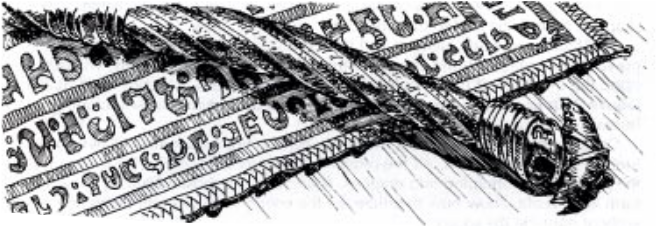
\includegraphics[width=\textwidth-25mm]{images/filler-1.png}
\WOTC
\end{center}
}
\section{Spell Descriptions}
The spells herein are presented in alphabetical order (with the exception of those whose names begin with ``greater,'' ``lesser,'' or ``mass''; see Order of Presentation).
\end{strip}

\Spell{Acid Arrow}{acid arrow}
{Conjuration (Creation) [Acid]}
{
	\textbf{Level:}
	Wiz 2\\
	\textbf{Components:}
	V, S, M, F\\
	\textbf{Casting Time:}
	1 standard action\\
	\textbf{Range:}
	Long (120 m + 12 m/level)\\
	\textbf{Effect:}
	One arrow of acid\\
	\textbf{Duration:}
	1 round + 1 round per three levels\\
	\textbf{Saving Throw:}
	None\\
	\textbf{Spell Resistance:}
	No\\
}
{
	A magical arrow of acid springs from your hand and speeds to its target. You must succeed on a ranged touch attack to hit your target. The arrow deals 2d4 points of acid damage with no splash damage. For every three caster levels (to a maximum of 18th), the acid, unless somehow neutralized, lasts for another round, dealing another 2d4 points of damage in that round.

	\textit{Material Component}:
	Powdered rhubarb leaf and an adder's stomach.

	\textit{Focus}:
	A dart.

}

\Spell{Acid Fog}{acid fog}
{Conjuration (Creation) [Acid]}
{
	\textbf{Level:}
	Wiz 6\\
	\textbf{Components:}
	V, S, M\\
	\textbf{Casting Time:}
	1 standard action\\
	\textbf{Range:}
	Medium (30 m + 3 m/level)\\
	\textbf{Effect:}
	Fog spreads in 6-m radius, 6 m high\\
	\textbf{Duration:}
	1 round/level\\
	\textbf{Saving Throw:}
	None\\
	\textbf{Spell Resistance:}
	No\\
}
{
	\emph{Acid fog} creates a billowing mass of misty vapors similar to that produced by a \spell{solid fog} spell. In addition to slowing creatures down and obscuring sight, this spell's vapors are highly acidic. Each round on your turn, starting when you cast the spell, the fog deals 2d6 points of acid damage to each creature and object within it.

	\textit{Arcane Material Component:}
	A pinch of dried, powdered peas combined with powdered animal hoof.

}

\Spell{Acid Splash}{acid splash}
{Conjuration (Creation) [Acid]}
{
	\textbf{Level:}
	Wiz 0\\
	\textbf{Components:}
	V, S\\
	\textbf{Casting Time:}
	1 standard action\\
	\textbf{Range:}
	Close (7.5 m + 1.5 m/2 levels)\\
	\textbf{Effect:}
	One missile of acid\\
	\textbf{Duration:}
	Instantaneous\\
	\textbf{Saving Throw:}
	None\\
	\textbf{Spell Resistance:}
	No\\
}
{
	You fire a small orb of acid at the target. You must succeed on a ranged touch attack to hit your target. The orb deals 1d3 points of acid damage.

}

\Spell{Aid}{aid}
{Enchantment (Compulsion) [Mind-Affecting]}
{
	\textbf{Level}: Clr 2\\
	\textbf{Components}: V, S, DF\\
	\textbf{Casting Time}: 1 standard action\\
	\textbf{Range}: Touch\\
	\textbf{Target}: Living creature touched\\
	\textbf{Duration}: 1 min./level\\
	\textbf{Saving Throw}: None\\
	\textbf{Spell Resistance}: Yes (harmless)\\
}
{
	Aid grants the target a +1 morale bonus on attack rolls and saves against fear effects, plus temporary hit points equal to 1d8 + caster level (to a maximum of 1d8+10 temporary hit points at caster level 10th).
}
\Spell{Air Walk}{air walk}
{Transmutation [Air]}
{
	\textbf{Level}: Clr 4, Drd 4, Freedom 2, Tmp 4\\
	\textbf{Components}: V, S, DF\\
	\textbf{Casting Time}: 1 standard action\\
	\textbf{Range}: Touch\\
	\textbf{Target}: Creature (Gargantuan or smaller) touched\\
	\textbf{Duration}: 10 min./level\\
	\textbf{Saving Throw}: None\\
	\textbf{Spell Resistance}: Yes (harmless)\\
}
{
	The subject can tread on air as if walking on solid ground. Moving upward is similar to walking up a hill. The maximum upward or downward angle possible is 45 degrees, at a rate equal to one-half the air walker’s normal speed.

	A strong wind (21+ mph) can push the subject along or hold it back. At the end of its turn each round, the wind blows the air walker 1.5 meter for each 1.5 kilometer per hour of wind speed. The creature may be subject to additional penalties in exceptionally strong or turbulent winds, such as loss of control over movement or physical damage from being buffeted about.

	Should the spell duration expire while the subject is still aloft, the magic fails slowly. The subject floats downward 18 meters per round for 1d6 rounds. If it reaches the ground in that amount of time, it lands safely. If not, it falls the rest of the distance, taking 1d6 points of damage per 3 meters of fall. Since dispelling a spell effectively ends it, the subject also descends in this way if the air walk spell is dispelled, but not if it is negated by an antimagic field.

	You can cast air walk on a specially trained mount so it can be ridden through the air. You can train a mount to move with the aid of air walk (counts as a trick; see \skill{Handle Animal} skill) with one week of work and a DC 25 \skill{Handle Animal} check.
}
\Spell{Alarm}{alarm}
{Abjuration}
{
	\textbf{Level:}
	Rgr 1, Wiz 1\\
	\textbf{Components:}
	V, S, F/DF\\
	\textbf{Casting Time:}
	1 standard action\\
	\textbf{Range:}
	Close (7.5 m + 1.5 m/2 levels)\\
	\textbf{Area:}
	6-m-radius emanation centered on a point in space\\
	\textbf{Duration:}
	2 hours/level (D)\\
	\textbf{Saving Throw:}
	None\\
	\textbf{Spell Resistance:}
	No\\
}
{
	Alarm sounds a mental or audible alarm each time a creature of Tiny or larger size enters the warded area or touches it. A creature that speaks the password (determined by you at the time of casting) does not set off the alarm. You decide at the time of casting whether the alarm will be mental or audible.

	\textit{Mental Alarm:}
	A mental alarm alerts you (and only you) so long as you remain within 1.5 kilometer of the warded area. You note a single mental ``ping'' that awakens you from normal sleep but does not otherwise disturb concentration. A silence spell has no effect on a mental alarm.

	\textit{Audible Alarm:}
	An audible alarm produces the sound of a hand bell, and anyone within 18 meters of the warded area can hear it clearly. Reduce the distance by 3 meters for each interposing closed door and by 6 meters for each substantial interposing wall.

	In quiet conditions, the ringing can be heard faintly as far as 54 meters away. The sound lasts for 1 round. Creatures within a silence spell cannot hear the ringing.

	Ethereal or astral creatures do not trigger the alarm.

	\emph{Alarm} can be made permanent with a \spell{permanency} spell.

	\textit{Arcane Focus:}
	A tiny bell and a piece of very fine silver wire.

}

\Spell{Align Weapon}{align weapon}
{Transmutation [see text]}
{
	\textbf{Level:}
	Clr 2\\
	\textbf{Components:}
	V, S, DF\\
	\textbf{Casting Time:}
	1 standard action\\
	\textbf{Range:}
	Touch\\
	\textbf{Target:}
	Weapon touched or fifty projectiles (all of which must be in contact with each other at the time of casting)\\
	\textbf{Duration:}
	1 min./level\\
	\textbf{Saving Throw:}
	Will negates (harmless, object)\\
	\textbf{Spell Resistance:}
	Yes (harmless, object)\\
}
{
	Align weapon makes a weapon good, evil, lawful, or chaotic, as you choose. A weapon that is aligned can bypass the damage reduction of certain creatures. This spell has no effect on a weapon that already has an alignment.

	You can't cast this spell on a natural weapon, such as an unarmed strike.

	When you make a weapon good, evil, lawful, or chaotic, align weapon is a good, evil, lawful, or chaotic spell, respectively.

}

\Spell{Alter Self}{alter self}
{Transmutation}
{
	\textbf{Level:}
	Ass 2, Wiz 2\\
	\textbf{Components:}
	V, S\\
	\textbf{Casting Time:}
	1 standard action\\
	\textbf{Range:}
	Personal\\
	\textbf{Target:}
	You\\
	\textbf{Duration:}
	10 min./level (D)\\
}
{
	You assume the form of a creature of the same type as your normal form. The new form must be within one size category of your normal size. The maximum HD of an assumed form is equal to your caster level, to a maximum of 5 HD at 5th level. You can change into a member of your own kind or even into yourself.

	You retain your own ability scores. Your class and level, hit points, alignment, base attack bonus, and base save bonuses all remain the same. You retain all supernatural and spell-like special attacks and qualities of your normal form, except for those requiring a body part that the new form does not have (such as a mouth for a breath weapon or eyes for a gaze attack).

	You keep all extraordinary special attacks and qualities derived from class levels, but you lose any from your normal form that are not derived from class levels.

	If the new form is capable of speech, you can communicate normally. You retain any spellcasting ability you had in your original form, but the new form must be able to speak intelligibly (that is, speak a language) to use verbal components and must have limbs capable of fine manipulation to use somatic or material components.

	You acquire the physical qualities of the new form while retaining your own mind. Physical qualities include natural size, mundane movement capabilities (such as burrowing, climbing, walking, swimming, and flight with wings, to a maximum speed of 36 meters for flying or 18 meters for nonflying movement), natural armor bonus, natural weapons (such as claws, bite, and so on), racial skill bonuses, racial bonus feats, and any gross physical qualities (presence or absence of wings, number of extremities, and so forth). A body with extra limbs does not allow you to make more attacks (or more advantageous two-weapon attacks) than normal.

	You do not gain any extraordinary special attacks or special qualities not noted above under physical qualities, such as darkvision, low-light vision, blindsense, blindsight, fast healing, regeneration, scent, and so forth.

	You do not gain any supernatural special attacks, special qualities, or spell-like abilities of the new form. Your creature type and subtype (if any) remain the same regardless of your new form. You cannot take the form of any creature with a template, even if that template doesn't change the creature type or subtype.

	You can freely designate the new form's minor physical qualities (such as hair color, hair texture, and skin color) within the normal ranges for a creature of that kind. The new form's significant physical qualities (such as height, weight, and gender) are also under your control, but they must fall within the norms for the new form's kind. You are effectively disguised as an average member of the new form's race. If you use this spell to create a disguise, you get a +10 bonus on your \skill{Disguise} check.

	When the change occurs, your equipment, if any, either remains worn or held by the new form (if it is capable of wearing or holding the item), or melds into the new form and becomes nonfunctional. When you revert to your true form, any objects previously melded into the new form reappear in the same location on your body they previously occupied and are once again functional. Any new items you wore in the assumed form and can't wear in your normal form fall off and land at your feet; any that you could wear in either form or carry in a body part common to both forms at the time of reversion are still held in the same way. Any part of the body or piece of equipment that is separated from the whole reverts to its true form.

}

\Spell{Analyze Dweomer}{analyze dweomer}
{Divination}
{
	\textbf{Level:}
	Wiz 6\\
	\textbf{Components:}
	V, S, F\\
	\textbf{Casting Time:}
	1 standard action\\
	\textbf{Range:}
	Close (7.5 m + 1.5 m/2 levels)\\
	\textbf{Targets:}
	One object or creature per caster level\\
	\textbf{Duration:}
	1 round/level (D)\\
	\textbf{Saving Throw:}
	None or Will negates; see text\\
	\textbf{Spell Resistance:}
	No\\
}
{
	You discern all spells and magical properties present in a number of creatures or objects. Each round, you may examine a single creature or object that you can see as a free action. In the case of a magic item, you learn its functions, how to activate its functions (if appropriate), and how many charges are left (if it uses charges). In the case of an object or creature with active spells cast upon it, you learn each spell, its effect, and its caster level.

	An attended object may attempt a Will save to resist this effect if its holder so desires. If the save succeeds, you learn nothing about the object except what you can discern by looking at it. An object that makes its save cannot be affected by any other analyze dweomer spells for 24 hours.

	Analyze dweomer does not function when used on an artifact.

	\textit{Focus:}
	A tiny lens of ruby or sapphire set in a small golden loop. The gemstone must be worth at least 1,500 cp.

}

\Spell{Animal Growth}{animal growth}
{Transmutation}
{
	\textbf{Level:}
	Drd 5, Rgr 4, Wiz 5\\
	\textbf{Components:}
	V, S\\
	\textbf{Casting Time:}
	1 standard action\\
	\textbf{Range:}
	Medium (30 m + 3 m/level)\\
	\textbf{Targets:}
	Up to one animal (Gargantuan or smaller) per two levels, no two of which can be more than 9 m apart\\
	\textbf{Duration:}
	1 min./level\\
	\textbf{Saving Throw:}
	Fortitude negates\\
	\textbf{Spell Resistance:}
	Yes\\
}
{
	A number of animals grow to twice their normal size and eight times their normal weight. This alteration changes each animal's size category to the next largest, grants it a +8 size bonus to Strength and a +4 size bonus to Constitution (and thus an extra 2 hit points per HD), and imposes a $-2$ size penalty to Dexterity. The creature's existing natural armor bonus increases by 2. The size change also affects the animal's modifier to AC and attack rolls and its base damage. The animal's space and reach change as appropriate to the new size, but its speed does not change.

	The spell also grants each subject damage reduction 10/magic and a +4 resistance bonus on saving throws. If insufficient room is available for the desired growth, the creature attains the maximum possible size and may make a Strength check (using its increased Strength) to burst any enclosures in the process. If it fails, it is constrained without harm by the materials enclosing it--- the spell cannot be used to crush a creature by increasing its size.

	All equipment worn or carried by an animal is similarly enlarged by the spell, though this change has no effect on the magical properties of any such equipment.

	Any enlarged item that leaves the enlarged creature's possession instantly returns to its normal size.

	The spell gives no means of command or influence over the enlarged animals.

	Multiple magical effects that increase size do not stack.

}

\Spell{Animal Messenger}{animal messenger}
{Enchantment (Compulsion) [Mind-Affecting]}
{
	\textbf{Level:}
	Drd 2, Rgr 1\\
	\textbf{Components:}
	V, S, M\\
	\textbf{Casting Time:}
	1 standard action\\
	\textbf{Range:}
	Close (7.5 m + 1.5 m/2 levels)\\
	\textbf{Target:}
	One Tiny animal\\
	\textbf{Duration:}
	One day/level\\
	\textbf{Saving Throw:}
	None; see text\\
	\textbf{Spell Resistance:}
	Yes\\
}
{
	You compel a Tiny animal to go to a spot you designate. The most common use for this spell is to get an animal to carry a message to your allies. The animal cannot be one tamed or trained by someone else, including such creatures as familiars and animal companions.

	Using some type of food desirable to the animal as a lure, you call the animal to you. It advances and awaits your bidding. You can mentally impress on the animal a certain place well known to you or an obvious landmark. The directions must be simple, because the animal depends on your knowledge and can't find a destination on its own. You can attach some small item or note to the messenger. The animal then goes to the designated location and waits there until the duration of the spell expires, whereupon it resumes its normal activities.

	During this period of waiting, the messenger allows others to approach it and remove any scroll or token it carries. The intended recipient gains no special ability to communicate with the animal or read any attached message (if it's written in a language he or she doesn't know, for example).

	\textit{Material Component}:
	A morsel of food the animal likes.

}

\Spell{Animal Shapes}{animal shapes}
{Transmutation}
{
	\textbf{Level:}
	Animal 7, Drd 8\\
	\textbf{Components:}
	V, S, DF\\
	\textbf{Casting Time:}
	1 standard action\\
	\textbf{Range:}
	Close (7.5 m + 1.5 m/2 levels)\\
	\textbf{Targets:}
	Up to one willing creature per level, all within 9 m of each other\\
	\textbf{Duration:}
	1 hour/level (D)\\
	\textbf{Saving Throw:}
	None; see text\\
	\textbf{Spell Resistance:}
	Yes (harmless)\\
}
{
	You transform up to one willing creature per caster level into an animal of your choice; the spell has no effect on unwilling creatures. Use the alternate form special ability to determine each target's new abilities. All creatures must take the same kind of animal form. Recipients remain in the animal form until the spell expires or until you dismiss it for all recipients. In addition, an individual subject may choose to resume its normal form as a full-round action; doing so ends the spell for that subject alone. The maximum HD of an assumed form is equal to the subject's HD or your caster level, whichever is lower, to a maximum of 20 HD at 20th level.

}

\Spell{Animal Trance}{animal trance}
{Enchantment (Compulsion) [Mind-Affecting, Sonic]}
{
	\textbf{Level:}
	Drd 2\\
	\textbf{Components:}
	V, S\\
	\textbf{Casting Time:}
	1 standard action\\
	\textbf{Range:}
	Close (7.5 m + 1.5 m/2 levels)\\
	\textbf{Targets:}
	Animals or magical beasts with Intelligence 1 or 2\\
	\textbf{Duration:}
	Concentration\\
	\textbf{Saving Throw:}
	Will negates; see text\\
	\textbf{Spell Resistance:}
	Yes\\
}
{
	Your swaying motions and music (or singing, or chanting) compel animals and magical beasts to do nothing but watch you. Only a creature with an Intelligence score of 1 or 2 can be fascinated by this spell. Roll 2d6 to determine the total number of HD worth of creatures that you fascinate. The closest targets are selected first until no more targets within range can be affected.

	A magical beast, a dire animal, or an animal trained to attack or guard is allowed a saving throw; an animal not trained to attack or guard is not.

}

\Spell{Animate Dead}{animate dead}
{Necromancy [Evil]}
{
	\textbf{Level:}
	Clr 3, Death 3, Wiz 4\\
	\textbf{Components:}
	V, S, M\\
	\textbf{Casting Time:}
	1 standard action\\
	\textbf{Range:}
	Touch\\
	\textbf{Targets:}
	One or more corpses touched\\
	\textbf{Duration:}
	Instantaneous\\
	\textbf{Saving Throw:}
	None\\
	\textbf{Spell Resistance:}
	No\\
}
{
	This spell turns the bones or bodies of dead creatures into undead skeletons or zombies that follow your spoken commands.

	The undead can follow you, or they can remain in an area and attack any creature (or just a specific kind of creature) entering the place. They remain animated until they are destroyed. (A destroyed skeleton or zombie can't be animated again.)

	Regardless of the type of undead you create with this spell, you can't create more HD of undead than twice your caster level with a single casting of animate dead. (The \spell{desecrate} spell doubles this limit)

	The undead you create remain under your control indefinitely. No matter how many times you use this spell, however, you can control only 4 HD worth of undead creatures per caster level. If you exceed this number, all the newly created creatures fall under your control, and any excess undead from previous castings become uncontrolled. (You choose which creatures are released.) If you are a cleric, any undead you might command by virtue of your power to command or rebuke undead do not count toward the limit.

	\textit{Skeletons:}
	A skeleton can be created only from a mostly intact corpse or skeleton. The corpse must have bones. If a skeleton is made from a corpse, the flesh falls off the bones.

	\textit{Zombies:}
	A zombie can be created only from a mostly intact corpse. The corpse must be that of a creature with a true anatomy.

	\textit{Material Component:}
	You must place a black onyx gem worth at least 25 cp per Hit Die of the undead into the mouth or eye socket of each corpse you intend to animate. The magic of the spell turns these gems into worthless, burned-out shells.

}

\Spell{Animate Objects}{animate objects}
{Transmutation}
{
	\textbf{Level:}
	Chaos 6, Clr 6\\
	\textbf{Components:}
	V, S\\
	\textbf{Casting Time:}
	1 standard action\\
	\textbf{Range:}
	Medium (30 m + 3 m/level)\\
	\textbf{Targets:}
	One Small object per caster level; see text\\
	\textbf{Duration:}
	1 round/level\\
	\textbf{Saving Throw:}
	None\\
	\textbf{Spell Resistance:}
	No\\
}
{
	You imbue inanimate objects with mobility and a semblance of life. Each such animated object then immediately attacks whomever or whatever you initially designate.

	An animated object can be of any nonmagical material. You may animate one Small or smaller object or an equivalent number of larger objects per caster level. A Medium object counts as two Small or smaller objects, a Large object as four, a Huge object as eight, a Gargantuan object as sixteen, and a Colossal object as thirty-two. You can change the designated target or targets as a move action, as if directing an active spell.

	This spell cannot animate objects carried or worn by a creature.

	Animate objects can be made permanent with a \spell{permanency} spell.

}

\Spell{Animate Plants}{animate plants}
{Transmutation}
{
	\textbf{Level:}
	Drd 7, Growth 7, Plant 7\\
	\textbf{Components:}
	V\\
	\textbf{Casting Time:}
	1 standard action\\
	\textbf{Range:}
	Close (7.5 m + 1.5 m/2 levels)\\
	\textbf{Targets:}
	One Large plant per three caster levels or all plants within range; see text\\
	\textbf{Duration:}
	1 round/level or 1 hour/level; see text\\
	\textbf{Saving Throw:}
	None\\
	\textbf{Spell Resistance:}
	No\\
}
{
	You imbue inanimate plants with mobility and a semblance of life. Each animated plant then immediately attacks whomever or whatever you initially designate as though it were an animated object of the appropriate size category. You may animate one Large or smaller plant, or an equivalent number of larger plants, per three caster levels. A Huge plant counts as two Large or smaller plants, a Gargantuan plant as four, and a Colossal plant as eight. You can change the designated target or targets as a move action, as if directing an active spell.

	Use the statistics for animated objects, except that plants smaller than Large usually don't have hardness.

	Animate plants cannot affect plant creatures, nor does it affect nonliving vegetable material.

	\textit{Entangle}:
	Alternatively, you may imbue all plants within range with a degree of mobility, which allows them to entwine around creatures in the area. This usage of the spell duplicates the effect of an entangle spell. Spell resistance does not keep creatures from being entangled. This effect lasts 1 hour per caster level.

}

\Spell{Animate Rope}{animate rope}
{Transmutation}
{
	\textbf{Level:}
	Wiz 1\\
	\textbf{Components:}
	V, S\\
	\textbf{Casting Time:}
	1 standard action\\
	\textbf{Range:}
	Medium (30 m + 3 m/level)\\
	\textbf{Target:}
	One ropelike object, length up to 15 m + 1.5 m/level; see text\\
	\textbf{Duration:}
	1 round/level\\
	\textbf{Saving Throw:}
	None\\
	\textbf{Spell Resistance:}
	No\\
}
{
	You can animate a nonliving ropelike object. The maximum length assumes a rope with a 2-centimeter diameter.

	Reduce the maximum length by 50\% for every additional 2.5 centimeters of thickness, and increase it by 50\% for each reduction of the rope's diameter by half.

	The possible commands are ``coil'' (form a neat, coiled stack), ``coil and knot,'' ``loop,'' ``loop and knot,'' ``tie and knot,'' and the opposites of all of the above (``uncoil,'' and so forth). You can give one command each round as a move action, as if directing an active spell.

	The rope can enwrap only a creature or an object within 30 centimeters of it---it does not snake outward---so it must be thrown near the intended target. Doing so requires a successful ranged touch attack roll (range increment 3 meters). A typical 2-centimeter-diameter hempen rope has 2 hit points, AC 10, and requires a DC 23 Strength check to burst it. The rope does not deal damage, but it can be used as a trip line or to cause a single opponent that fails a Reflex saving throw to become entangled. A creature capable of spellcasting that is bound by this spell must make a DC 15 \skill{Concentration} check to cast a spell. An entangled creature can slip free with a DC 20 \skill{Escape Artist} check.

	The rope itself and any knots tied in it are not magical.

	This spell grants a +2 bonus on any \skill{Use Rope} checks you make when using the transmuted rope.

	The spell cannot animate objects carried or worn by a creature.

}

\Spell{Antilife Shell}{antilife shell}
{Abjuration}
{
	\textbf{Level:}
	Animal 6, Clr 6, Drd 6\\
	\textbf{Components:}
	V, S, DF\\
	\textbf{Casting Time:}
	1 round\\
	\textbf{Range:}
	3 m\\
	\textbf{Area:}
	3-m-radius emanation, centered on you\\
	\textbf{Duration:}
	10 min./level (D)\\
	\textbf{Saving Throw:}
	None\\
	\textbf{Spell Resistance:}
	Yes\\
}
{
	You bring into being a mobile, hemispherical energy field that prevents the entrance of most types of living creatures.

	The effect hedges out animals, aberrations, dragons, fey, giants, humanoids, magical beasts, monstrous humanoids, oozes, plants, and vermin, but not constructs, elementals, outsiders, or undead.

	This spell may be used only defensively, not aggressively. Forcing an abjuration barrier against creatures that the spell keeps at bay collapses the barrier.

}

\Spell{Antimagic Field}{antimagic field}
{Abjuration}
{
	\textbf{Level:}
	Clr 8, Magic 6, Purity 8, Protection 6, ~~~ Wiz 6\\
	\textbf{Components:}
	V, S, M/DF\\
	\textbf{Casting Time:}
	1 standard action\\
	\textbf{Range:}
	3 m\\
	\textbf{Area:}
	3-m-radius emanation, centered on you\\
	\textbf{Duration:}
	10 min./level (D)\\
	\textbf{Saving Throw:}
	None\\
	\textbf{Spell Resistance:}
	See text\\
}
{
	An invisible barrier surrounds you and moves with you. The space within this barrier is impervious to most magical effects, including spells, spell-like abilities, and supernatural abilities. Likewise, it prevents the functioning of any magic items or spells within its confines.

	An \emph{antimagic field} suppresses any spell or magical effect used within, brought into, or cast into the area, but does not dispel it. Time spent within an \emph{antimagic field} counts against the suppressed spell's duration.

	Summoned creatures of any type and incorporeal undead wink out if they enter an \emph{antimagic field}. They reappear in the same spot once the field goes away. Time spent winked out counts normally against the duration of the conjuration that is maintaining the creature. If you cast \emph{antimagic field} in an area occupied by a summoned creature that has spell resistance, you must make a caster level check (1d20 + caster level) against the creature's spell resistance to make it wink out. (The effects of instantaneous conjurations are not affected by an \emph{antimagic field} because the conjuration itself is no longer in effect, only its result.)

	A normal creature can enter the area, as can normal missiles. Furthermore, while a magic sword does not function magically within the area, it is still a sword (and a masterwork sword at that). The spell has no effect on golems and other constructs that are imbued with magic during their creation process and are thereafter self-supporting (unless they have been summoned, in which case they are treated like any other summoned creatures). Elementals, corporeal undead, and outsiders are likewise unaffected unless summoned. These creatures' spell-like or supernatural abilities, however, may be temporarily nullified by the field. \spell{Dispel Magic} does not remove the field, though \spell{Mage's Disjunction} might.

	Two or more \emph{antimagic fields} sharing any of the same space have no effect on each other. Certain spells, such as \spell{wall of force}, \spell{prismatic sphere}, and \spell{prismatic wall}, remain unaffected by antimagic field (see the individual spell descriptions). Artifacts and deities are unaffected by mortal magic such as this.

	Should a creature be larger than the area enclosed by the barrier, any part of it that lies outside the barrier is unaffected by the field.

	\textit{Arcane Material Component}:
	A pinch of powdered iron or iron filings.

}

\Spell{Antipathy}{antipathy}
{Enchantment (Compulsion) [Mind-Affecting]}
{
	\textbf{Level:}
	Agriculture 8, Drd 9, Tmp 8, Wiz 8\\
	\textbf{Components:}
	V, S, M/DF\\
	\textbf{Casting Time:}
	1 hour\\
	\textbf{Range:}
	Close (7.5 m + 1.5 m/2 levels)\\
	\textbf{Target:}
	One location (up to a 3-m cube/level) or one object\\
	\textbf{Duration:}
	2 hours/level (D)\\
	\textbf{Saving Throw:}
	Will partial\\
	\textbf{Spell Resistance:}
	Yes\\
}
{
	You cause an object or location to emanate magical vibrations that repel either a specific kind of intelligent creature or creatures of a particular alignment, as defined by you. The kind of creature to be affected must be named specifically. A creature subtype is not specific enough. Likewise, the specific alignment to be repelled must be named.

	Creatures of the designated kind or alignment feel an overpowering urge to leave the area or to avoid the affected item.

	A compulsion forces them to abandon the area or item, shunning it and never willingly returning to it while the spell is in effect. A creature that makes a successful saving throw can stay in the area or touch the item but feels uncomfortable doing so. This distracting discomfort reduces the creature's Dexterity score by 4 points.

	\emph{Antipathy} counters and dispels \spell{sympathy}.

	\textit{Arcane Material Component}:
	A lump of alum soaked in vinegar.

}

\Spell{Antiplant Shell}{antiplant shell}
{Abjuration}
{
	\textbf{Level:}
	Drd 4\\
	\textbf{Components:}
	V, S, DF\\
	\textbf{Casting Time:}
	1 standard action\\
	\textbf{Range:}
	3 m\\
	\textbf{Area:}
	3-m-radius emanation, centered on you\\
	\textbf{Duration:}
	10 min./level (D)\\
	\textbf{Saving Throw:}
	None\\
	\textbf{Spell Resistance:}
	Yes\\
}
{
	The antiplant shell spell creates an invisible, mobile barrier that keeps all creatures within the shell protected from attacks by plant creatures or animated plants. As with many abjuration spells, forcing the barrier against creatures that the spell keeps at bay strains and collapses the field.

}

\Spell{Arcane Eye}{arcane eye}
{Divination (Scrying)}
{
	\textbf{Level:}
	Wiz 4\\
	\textbf{Components:}
	V, S, M\\
	\textbf{Casting Time:}
	10 minutes\\
	\textbf{Range:}
	Unlimited\\
	\textbf{Effect:}
	Magical sensor\\
	\textbf{Duration:}
	1 min./level (D)\\
	\textbf{Saving Throw:}
	None\\
	\textbf{Spell Resistance:}
	No\\
}
{
	You create an invisible magical sensor that sends you visual information. You can create the arcane eye at any point you can see, but it can then travel outside your line of sight without hindrance. An arcane eye travels at 9 meters per round (90 meters per minute) if viewing an area ahead as a human would (primarily looking at the floor) or 3 meters per round (30 meters per minute) if examining the ceiling and walls as well as the floor ahead. It sees exactly as you would see if you were there.

	The eye can travel in any direction as long as the spell lasts. Solid barriers block its passage, but it can pass through a hole or space as small as 1 inch in diameter. The eye can't enter another plane of existence, even through a \spell{gate} or similar magical portal.

	You must concentrate to use an arcane eye. If you do not concentrate, the eye is inert until you again concentrate.

	\textit{Material Component:}
	A bit of bat fur.

}

\Spell{Arcane Lock}{arcane lock}
{Abjuration}
{
	\textbf{Level:}
	Wiz 2\\
	\textbf{Components:}
	V, S, M\\
	\textbf{Casting Time:}
	1 standard action\\
	\textbf{Range:}
	Touch\\
	\textbf{Target:}
	The door, chest, or portal touched, up to 9 sq. m/level in size\\
	\textbf{Duration:}
	Permanent\\
	\textbf{Saving Throw:}
	None\\
	\textbf{Spell Resistance:}
	No\\
}
{
	An \emph{arcane lock} spell cast upon a door, chest, or portal magically locks it. You can freely pass your own \emph{arcane lock} without affecting it; otherwise, a door or object secured with this spell can be opened only by breaking in or with a successful \spell{dispel magic} or \spell{knock} spell. Add 10 to the normal DC to break open a door or portal affected by this spell. (A \spell{knock} spell does not remove an \emph{arcane lock}; it only suppresses the effect for 10 minutes.)

	\textit{Material Component}:
	Gold dust worth 25 gp.

}

\Spell{Arcane Mark}{arcane mark}
{Universal}
{
	\textbf{Level:}
	Wiz 0\\
	\textbf{Components:}
	V, S\\
	\textbf{Casting Time:}
	1 standard action\\
	\textbf{Range:}
	0 m\\
	\textbf{Effect:}
	One personal rune or mark, all of which must fit within 0.3 sq. m\\
	\textbf{Duration:}
	Permanent\\
	\textbf{Saving Throw:}
	None\\
	\textbf{Spell Resistance:}
	No\\
}
{
	This spell allows you to inscribe your personal rune or mark, which can consist of no more than six characters. The writing can be visible or invisible. An \emph{arcane mark} spell enables you to etch the rune upon any substance without harm to the material upon which it is placed. If an invisible mark is made, a detect magic spell causes it to glow and be visible, though not necessarily understandable.

	The spells \spell{see invisibility} and \spell{true seeing}, or the items gem of seeing and robe of eyes likewise allow the user to see an invisible \emph{arcane mark}. A \spell{read magic} spell reveals the words, if any. The mark cannot be dispelled, but it can be removed by the caster or by an erase spell.

	If an \emph{arcane mark} is placed on a living being, normal wear gradually causes the effect to fade in about a month.

	\emph{Arcane mark} must be cast on an object prior to casting instant summons on the same object (see that spell description for details).

}

\Spell{Arcane Sight}{arcane sight}
{Divination}
{
	\textbf{Level:}
	Wiz 3\\
	\textbf{Components:}
	V, S\\
	\textbf{Casting Time:}
	1 standard action\\
	\textbf{Range:}
	Personal\\
	\textbf{Target:}
	You\\
	\textbf{Duration:}
	1 min./level (D)\\
}
{
	This spell makes your eyes glow blue and allows you to see magical auras within 36 meters of you. The effect is similar to that of a detect magic spell, but arcane sight does not require concentration and discerns aura location and power more quickly.

	You know the location and power of all magical auras within your sight. An aura's power depends on a spell's functioning level or an item's caster level, as noted in the description of the detect magic spell. If the items or creatures bearing the auras are in line of sight, you can make \skill{Spellcraft} skill checks to determine the school of magic involved in each. (Make one check per aura; DC 15 + spell level, or 15 + one-half caster level for a nonspell effect.)

	If you concentrate on a specific creature within 36 meters of you as a standard action, you can determine whether it has any spellcasting or spell-like abilities, whether these are arcane or divine (spell-like abilities register as arcane), and the strength of the most powerful spell or spell-like ability the creature currently has available for use.

	Arcane sight can be made permanent with a \spell{permanency} spell.

}

\Spell{Arcane Sight, Greater}{arcane sight, greater}
{Divination}
{
	\textbf{Level:}
	Wiz 7\\
}
{
	This spell functions like \spell{arcane sight}, except that you automatically know which spells or magical effects are active upon any individual or object you see.

	Greater arcane sight doesn't let you identify magic items.

	Unlike \spell{arcane sight}, this spell cannot be made permanent with a \spell{permanency} spell.

}

\Spell{Astral Projection}{astral projection}
{Necromancy}
{
	\textbf{Level:}
	Clr 9, Wiz 9\\
	\textbf{Components:}
	V, S, M\\
	\textbf{Casting Time:}
	30 minutes\\
	\textbf{Range:}
	Touch\\
	\textbf{Targets:}
	You plus one additional willing creature touched per two caster levels\\
	\textbf{Duration:}
	See text\\
	\textbf{Saving Throw:}
	None\\
	\textbf{Spell Resistance:}
	Yes\\
}
{
	By freeing your spirit from your physical body, this spell allows you to project an astral body onto another plane altogether.

	You can bring the astral forms of other willing creatures with you, provided that these subjects are linked in a circle with you at the time of the casting. These fellow travelers are dependent upon you and must accompany you at all times. If something happens to you during the journey, your companions are stranded wherever you left them.

	You project your astral self onto the Astral Plane, leaving your physical body behind on the Material Plane in a state of suspended animation. The spell projects an astral copy of you and all you wear or carry onto the Astral Plane. Since the Astral Plane touches upon other planes, you can travel astrally to any of these other planes as you will. To enter one, you leave the Astral Plane, forming a new physical body (and equipment) on the plane of existence you have chosen to enter.

	While you are on the Astral Plane, your astral body is connected at all times to your physical body by a silvery cord. If the cord is broken, you are killed, astrally and physically. Luckily, very few things can destroy a silver cord. When a second body is formed on a different plane, the incorporeal silvery cord remains invisibly attached to the new body. If the second body or the astral form is slain, the cord simply returns to your body where it rests on the Material Plane, thereby reviving it from its state of suspended animation. Although astral projections are able to function on the Astral Plane, their actions affect only creatures existing on the Astral Plane; a physical body must be materialized on other planes.

	You and your companions may travel through the Astral Plane indefinitely. Your bodies simply wait behind in a state of suspended animation until you choose to return your spirits to them. The spell lasts until you desire to end it, or until it is terminated by some outside means, such as dispel magic cast upon either the physical body or the astral form, the breaking of the silver cord, or the destruction of your body back on the Material Plane (which kills you).

	\textit{Material Component}:
	A jacinth worth at least 1,000 cp, plus a silver bar worth 5 cp for each person to be affected.

}

\Spell{Atonement}{atonement}
{Abjuration [Ritual]}
{
	\textbf{Level:}
	Clr 5, Drd 5\\
	\textbf{Components:}
	V, S, M, F, DF, XP\\
	\textbf{Casting Time:}
	1 hour\\
	\textbf{Range:}
	Touch\\
	\textbf{Target:}
	Living creature touched\\
	\textbf{Duration:}
	Instantaneous\\
	\textbf{Saving Throw:}
	None\\
	\textbf{Spell Resistance:}
	Yes\\
}
{
	This spell removes the burden of evil acts or misdeeds from the subject. The creature seeking atonement must be truly repentant and desirous of setting right its misdeeds. If the atoning creature committed the evil act unwittingly or under some form of compulsion, \emph{atonement} operates normally at no cost to you. However, in the case of a creature atoning for deliberate misdeeds and acts of a knowing and willful nature, you must intercede with your deity (requiring you to expend 500 XP) in order to expunge the subject's burden. Many casters first assign a subject of this sort a quest (see geas/quest) or similar penance to determine whether the creature is truly contrite before casting the \emph{atonement} spell on its behalf.

	\emph{Atonement} may be cast for one of several purposes, depending on the version selected.

	\textit{Reverse Magical Alignment Change:}
	If a creature has had its alignment magically changed, \emph{atonement} returns its alignment to its original status at no cost in experience points.

	\textit{Restore Class:}
	An elemental champion or wanderer who has lost her class features due to committing a forbidden act may have her status restored to her by this spell.

	\textit{Restore Cleric or Druid Spell Powers:}
	A cleric or druid who has lost the ability to cast spells by incurring the anger of his or her deity may regain that ability by seeking atonement from another cleric of the same deity or another druid. If the transgression was intentional, the casting cleric loses 500 XP for his intercession. If the transgression was unintentional, he does not lose XP.

	\textit{Redemption or Temptation:}
	You may cast this spell upon a creature of an opposing alignment in order to offer it a chance to change its alignment to match yours. The prospective subject must be present for the entire casting process. Upon completion of the spell, the subject freely chooses whether it retains its original alignment or acquiesces to your offer and changes to your alignment. No duress, compulsion, or magical influence can force the subject to take advantage of the opportunity offered if it is unwilling to abandon its old alignment. This use of the spell does not work on outsiders or any creature incapable of changing its alignment naturally.

	Though the spell description refers to evil acts, \emph{atonement} can also be used on any creature that has performed acts against its alignment, whether those acts are evil, good, chaotic, or lawful.

	\textit{Note:} Normally, changing alignment is up to the player. This use of \emph{atonement} simply offers a believable way for a character to change his or her alignment drastically, suddenly, and definitively.

	\textit{Material Component:}
	Burning incense.

	\textit{Focus:}
	In addition to your holy symbol or normal divine focus, you need a set of prayer beads (or other prayer device, such as a prayer wheel or prayer book) worth at least 500 cp.

	\textit{XP Cost:}
	When cast for the benefit of a creature whose guilt was the result of deliberate acts, the cost to you is 500 XP per casting (see above).

}

\Spell{Augury}{augury}
{Divination}
{
	\textbf{Level:}
	Clr 2, Elemental Champion 2\\
	\textbf{Components:}
	V, S, M, F\\
	\textbf{Casting Time:}
	1 minute\\
	\textbf{Range:}
	Personal\\
	\textbf{Target:}
	You\\
	\textbf{Duration:}
	Instantaneous\\
}
{
	An augury can tell you whether a particular action will bring good or bad results for you in the immediate future.

	The base chance for receiving a meaningful reply is 70\% + 1\% per caster level, to a maximum of 90\%; this roll is made secretly. A question may be so straightforward that a successful result is automatic, or so vague as to have no chance of success. If the augury succeeds, you get one of four results:

\begin{itemize*}
\item Weal (if the action will probably bring good results).
\item Woe (for bad results).
\item Weal and woe (for both).
\item Nothing (for actions that don't have especially good or bad results).
\end{itemize*}

	If the spell fails, you get the ``nothing'' result. A cleric who gets the ``nothing'' result has no way to tell whether it was the consequence of a failed or successful augury.

	The augury can see into the future only about half an hour, so anything that might happen after that does not affect the result. Thus, the result might not take into account the long-term consequences of a contemplated action. All auguries cast by the same person about the same topic use the same dice result as the first casting.

	\textit{Material Component}:
	Incense worth at least 25 cp.

	\textit{Focus}:
	A set of marked sticks, bones, or similar tokens of at least 25 cp value.

}

\Spell{Awaken}{awaken}
{Transmutation}
{
	\textbf{Level:}
	Drd 5\\
	\textbf{Components:}
	V, S, DF, XP\\
	\textbf{Casting Time:}
	24 hours\\
	\textbf{Range:}
	Touch\\
	\textbf{Target:}
	Animal or tree touched\\
	\textbf{Duration:}
	Instantaneous\\
	\textbf{Saving Throw:}
	Will negates\\
	\textbf{Spell Resistance:}
	Yes\\
}
{
	You awaken a tree or animal to humanlike sentience. To succeed, you must make a Will save (DC 10 + the animal's current HD, or the HD the tree will have once awakened).

	The awakened animal or tree is friendly toward you. You have no special empathy or connection with a creature you awaken, although it serves you in specific tasks or endeavors if you communicate your desires to it.

	An awakened tree has characteristics as if it were an animated object, except that it gains the plant type and its Intelligence, Wisdom, and Charisma scores are each 3d6. An awakened plant gains the ability to move its limbs, roots, vines, creepers, and so forth, and it has senses similar to a human's.

	An awakened animal gets 3d6 Intelligence, +1d3 Charisma, and +2 HD. Its type becomes magical beast (augmented animal). An awakened animal can't serve as an animal companion, familiar, or special mount.

	An awakened tree or animal can speak one language that you know, plus one additional language that you know per point of Intelligence bonus (if any).

	\textit{XP Cost}:
	250 XP.

}

\Spell{Baleful Polymorph}{baleful polymorph}
{Transmutation}
{
	\textbf{Level:}
	Drd 5, Wiz 5\\
	\textbf{Components:}
	V, S\\
	\textbf{Casting Time:}
	1 standard action\\
	\textbf{Range:}
	Close (7.5 m + 1.5 m/2 levels)\\
	\textbf{Target:}
	One creature\\
	\textbf{Duration:}
	Permanent\\
	\textbf{Saving Throw:}
	Fortitude negates, Will partial; see text\\
	\textbf{Spell Resistance:}
	Yes\\
}
{
	You change the subject into a Small or smaller animal of no more than 1 HD (such as a dog, lizard, monkey, or toad). The subject takes on all the statistics and special abilities of an average member of the new form in place of its own except as follows:

\begin{itemize*}
\item The target retains its own alignment (and personality, within the limits of the new form's ability scores).
\item The target retains its own hit points.
\item The target is treated as having its normal Hit Dice for purpose of adjudicating effects based on HD, such as the sleep spell, though it uses the new form's base attack bonus, base save bonuses, and all other statistics derived from Hit Dice.
\item The target also retains the ability to understand (but not to speak) the languages it understood in its original form. It can write in the languages it understands, but only the form is capable of writing in some manner (such as drawing in the dirt with a paw).
\end{itemize*}

	With those exceptions, the target's normal game statistics are replaced by those of the new form. The target loses all the special abilities it has in its normal form, including its class features.

	All items worn or carried by the subject fall to the ground at its feet, even if they could be worn or carried by the new form.

	If the new form would prove fatal to the creature (for example, if you polymorphed a landbound target into a fish, or an airborne target into a toad), the subject gets a +4 bonus on the save.

	If the subject remains in the new form for 24 consecutive hours, it must attempt a Will save. If this save fails, it loses its ability to understand language, as well as all other memories of its previous form, and its Hit Dice and hit points change to match an average creature of its new form. These abilities and statistics return to normal if the effect is later ended.

	Incorporeal or gaseous creatures are immune to baleful polymorph, and a creature with the shapechanger subtype (such as a lycanthrope or a doppelganger) can revert to its natural form as a standard action (which ends the spell's effect).

}

\Spell{Bane}{bane}
{Enchantment (Compulsion) [Fear, Mind-Affecting]}
{
	\textbf{Level:}
	Clr 1\\
	\textbf{Components:}
	V, S, DF\\
	\textbf{Casting Time:}
	1 standard action\\
	\textbf{Range:}
	15 m\\
	\textbf{Area:}
	All enemies within 15 m\\
	\textbf{Duration:}
	1 min./level\\
	\textbf{Saving Throw:}
	Will negates\\
	\textbf{Spell Resistance:}
	Yes\\
}
{
	Bane fills your enemies with fear and doubt. Each affected creature takes a -1 penalty on attack rolls and a -1 penalty on saving throws against fear effects.

	Bane counters and dispels bless.

}

\Spell{Banishment}{banishment}
{Abjuration}
{
	\textbf{Level:}
	Clr 6, Wiz 7\\
	\textbf{Components:}
	V, S, F\\
	\textbf{Casting Time:}
	1 standard action\\
	\textbf{Range:}
	Close (7.5 m + 1.5 m/2 levels)\\
	\textbf{Targets:}
	One or more extraplanar creatures, no two of which can be more than 9 m apart\\
	\textbf{Duration:}
	Instantaneous\\
	\textbf{Saving Throw:}
	Will negates\\
	\textbf{Spell Resistance:}
	Yes\\
}
{
	A banishment spell is a more powerful version of the dismissal spell. It enables you to force extraplanar creatures out of your home plane. As many as 2 Hit Dice of creatures per caster level can be banished.

	You can improve the spell's chance of success by presenting at least one object or substance that the target hates, fears, or otherwise opposes. For each such object or substance, you gain a +1 bonus on your caster level check to overcome the target's spell resistance (if any), the saving throw DC increases by 2.

	Certain rare items might work twice as well as a normal item for the purpose of the bonuses (each providing a +2 bonus on the caster level check against spell resistance and increasing the save DC by 4).

	\textit{Arcane Focus}:
	Any item that is distasteful to the subject (optional, see above).

}

\Spell{Barkskin}{barkskin}
{Transmutation}
{
	\textbf{Level:}
	Drd 2, Rgr 2, Plant 2\\
	\textbf{Components:}
	V, S, DF\\
	\textbf{Casting Time:}
	1 standard action\\
	\textbf{Range:}
	Touch\\
	\textbf{Target:}
	Living creature touched\\
	\textbf{Duration:}
	10 min./level\\
	\textbf{Saving Throw:}
	None\\
	\textbf{Spell Resistance:}
	Yes (harmless)\\
}
{
	Barkskin toughens a creature's skin. The effect grants a +2 enhancement bonus to the creature's existing natural armor bonus. This enhancement bonus increases by 1 for every three caster levels above 3rd, to a maximum of +5 at caster level 12th.

	The enhancement bonus provided by barkskin stacks with the target's natural armor bonus, but not with other enhancement bonuses to natural armor. A creature without natural armor has an effective natural armor bonus of +0.

}

\Spell{Bear's Endurance}{bear's endurance}
{Transmutation}
{
	\textbf{Level:}
	Clr 2, Drd 2, Elemental Champion 1, Rgr 2, Tmp 2, Wiz 2\\
	\textbf{Components:}
	V, S, DF\\
	\textbf{Casting Time:}
	1 standard action\\
	\textbf{Range:}
	Touch\\
	\textbf{Target:}
	Creature touched\\
	\textbf{Duration:}
	1 min./level\\
	\textbf{Saving Throw:}
	Will negates (harmless)\\
	\textbf{Spell Resistance:}
	Yes\\
}
{
	The affected creature gains greater vitality and stamina. The spell grants the subject a +4 enhancement bonus to Constitution, which adds the usual benefits to hit points, Fortitude saves, Constitution checks, and so forth.

	Hit points gained by a temporary increase in Constitution score are not temporary hit points. They go away when the subject's Constitution drops back to normal. They are not lost first as temporary hit points are.

}

\Spell{Bear's Endurance, Mass}{mass bear's endurance}
{Transmutation}
{
	\textbf{Level:}
	Clr 6, Drd 6, Wiz 6\\
	\textbf{Range:}
	Close (7.5 m + 1.5 m/2 levels)\\
	\textbf{Targets:}
	One creature/level, no two of which can be more than 9 m apart\\
}
{
	Mass bear's endurance works like bear's endurance, except that it affects multiple creatures.

}

\Spell{Bestow Curse}{bestow curse}
{Necromancy}
{
	\textbf{Level:}
	Clr 3, Wiz 4\\
	\textbf{Components:}
	V, S\\
	\textbf{Casting Time:}
	1 standard action\\
	\textbf{Range:}
	Touch\\
	\textbf{Target:}
	Creature touched\\
	\textbf{Duration:}
	Permanent\\
	\textbf{Saving Throw:}
	Will negates\\
	\textbf{Spell Resistance:}
	Yes\\
}
{
	You place a curse on the subject. Choose one of the following three effects.
\begin{itemize*}
\item $-6$ decrease to an ability score (minimum 1).
\item $-4$ penalty on attack rolls, saves, ability checks, and skill checks.
\item Each turn, the target has a 50\% chance to act normally; otherwise, it takes no action.
\end{itemize*}

	You may also invent your own curse, but it should be no more powerful than those described above.

	The curse bestowed by this spell cannot be dispelled, but it can be removed with a break enchantment, limited wish, miracle, remove curse, or wish spell.

	Bestow curse counters remove curse.

}

\Spell{Binding}{binding}
{Enchantment (Compulsion) [Mind-Affecting]}
{
	\textbf{Level:}
	Wiz 8\\
	\textbf{Components:}
	V, S, M\\
	\textbf{Casting Time:}
	One minute\\
	\textbf{Range:}
	Close (7.5 m + 1.5 m/2 levels)\\
	\textbf{Target:}
	One living creature\\
	\textbf{Duration:}
	See text (D)\\
	\textbf{Saving Throw:}
	Will negates; see text\\
	\textbf{Spell Resistance:}
	Yes\\
}
{
	A binding spell creates a magical restraint to hold a creature. The target gets an initial saving throw only if its Hit Dice equal at least one-half your caster level.

	You may have as many as six assistants help you with the spell. For each assistant who casts suggestion, your caster level for this casting of binding increases by 1. For each assistant who casts dominate animal, dominate person, or dominate monster, your caster level for this casting of binding increases by a number equal to one-third of that assistant's level, provided that the spell's target is appropriate for a binding spell. Since the assistants' spells are cast simply to improve your caster level for the purpose of the binding spell, saving throws and spell resistance against the assistants' spells are irrelevant. Your caster level determines whether the target gets an initial Will saving throw and how long the binding lasts. All binding spells are dismissible.

	Regardless of the version of binding you cast, you can specify triggering conditions that end the spell and release the creature whenever they occur. These triggers can be as simple or elaborate as you desire, but the condition must be reasonable and have a likelihood of coming to pass. The conditions can be based on a creature's name, identity, or alignment but otherwise must be based on observable actions or qualities. Intangibles such as level, class, Hit Dice, or hit points don't qualify. Once the spell is cast, its triggering conditions cannot be changed. Setting a release condition increases the save DC (assuming a saving throw is allowed) by 2.

	If you are casting any of the first three versions of binding (those with limited durations), you may cast additional binding spells to prolong the effect, since the durations overlap. If you do so, the target gets a saving throw at the end of the first spell's duration, even if your caster level was high enough to disallow an initial saving throw. If the creature succeeds on this save, all the binding spells it has received are broken.

	The binding spell has six versions. Choose one of the following versions when you cast the spell.

	\textit{Chaining}:
	The subject is confined by restraints that generate an antipathy spell affecting all creatures who approach the subject, except you. The duration is one year per caster level. The subject of this form of binding is confined to the spot it occupied when it received the spell.

	\textit{Slumber}:
	This version causes the subject to become comatose for as long as one year per caster level. The subject does not need to eat or drink while slumbering, nor does it age. This form of binding is more difficult to cast than chaining, making it slightly easier to resist. Reduce the spell's save DC by 1.

	\textit{Bound Slumber}:
	This combination of chaining and slumber lasts for as long as one month per caster level. Reduce the save DC by 2.

	\textit{Hedged Prison}:
	The subject is transported to or otherwise brought within a confined area from which it cannot wander by any means. The effect is permanent. Reduce the save DC by 3.

	\textit{Metamorphosis}:
	The subject assumes gaseous form, except for its head or face. It is held harmless in a jar or other container, which may be transparent if you so choose. The creature remains aware of its surroundings and can speak, but it cannot leave the container, attack, or use any of its powers or abilities. The binding is permanent. The subject does not need to breathe, eat, or drink while metamorphosed, nor does it age. Reduce the save DC by 4.

	\textit{Minimus Containment}:
	The subject is shrunk to a height of 1 inch or even less and held within some gem, jar, or similar object. The binding is permanent. The subject does not need to breathe, eat, or drink while contained, nor does it age. Reduce the save DC by 4.

	You can't dispel a binding spell with dispel magic or a similar effect, though an antimagic field or Mage's disjunction affects it normally. A bound extraplanar creature cannot be sent back to its home plane due to dismissal, banishment, or a similar effect.

	\textit{Components}:
	The components for a binding spell vary according to the version of the spell, but they always include a continuous chanting utterance read from the scroll or spellbook page containing the spell, somatic gestures, and materials appropriate to the form of binding used. These components can include such items as miniature chains of special metals, soporific herbs of the rarest sort (for slumber bindings), a bell jar of the finest crystal, and the like

	In addition to the specially made props suited to the specific type of binding (cost 500 gp), the spell requires opals worth at least 500 gp for each HD of the target and a vellum depiction or carved statuette of the subject to be captured.

}

\Spell{Black Tentacles}{black tentacles}
{Conjuration (Creation)}
{
	\textbf{Level:}
	Wiz 4\\
	\textbf{Components:}
	V, S, M\\
	\textbf{Casting Time:}
	1 standard action\\
	\textbf{Range:}
	Medium (30 m + 3 m/level)\\
	\textbf{Area:}
	6-m-radius spread\\
	\textbf{Duration:}
	1 round/level (D)\\
	\textbf{Saving Throw:}
	None\\
	\textbf{Spell Resistance:}
	No\\
}
{
	This spell conjures a field of rubbery black tentacles, each 3 meters long. These waving members seem to spring forth from the earth, floor, or whatever surface is underfoot---including water. They grasp and entwine around creatures that enter the area, holding them fast and crushing them with great strength.

	Every creature within the area of the spell must make a grapple check, opposed by the grapple check of the tentacles. Treat the tentacles attacking a particular target as a Large creature with a base attack bonus equal to your caster level and a Strength score of 19. Thus, its grapple check modifier is equal to your caster level +8. The tentacles are immune to all types of damage.

	Once the tentacles grapple an opponent, they may make a grapple check each round on your turn to deal 1d6+4 points of bludgeoning damage. The tentacles continue to crush the opponent until the spell ends or the opponent escapes.

	Any creature that enters the area of the spell is immediately attacked by the tentacles. Even creatures who aren't grappling with the tentacles may move through the area at only half normal speed.

	\textit{Material Component}:
	A piece of tentacle from a giant octopus or a giant squid.

}

\Spell{Blade Barrier}{blade barrier}
{Evocation [Force]}
{
	\textbf{Level:}
	Clr 6, Good 6, War 6\\
	\textbf{Components:}
	V, S\\
	\textbf{Casting Time:}
	1 standard action\\
	\textbf{Range:}
	Medium (30 m + 3 m/level)\\
	\textbf{Effect:}
	Wall of whirling blades up to 6 m long/ level, or a ringed wall of whirling blades with a radius of up to 1.5 m per two levels; either form 6 m high\\
	\textbf{Duration:}
	1 min./level (D)\\
	\textbf{Saving Throw:}
	Reflex half or Reflex negates; see text\\
	\textbf{Spell Resistance:}
	Yes\\
}
{
	An immobile, vertical curtain of whirling blades shaped of pure force springs into existence. Any creature passing through the wall takes 1d6 points of damage per caster level (maximum 15d6), with a Reflex save for half damage.

	If you evoke the barrier so that it appears where creatures are, each creature takes damage as if passing through the wall. Each such creature can avoid the wall (ending up on the side of its choice) and thus take no damage by making a successful Reflex save.

	A blade barrier provides cover (+4 bonus to AC, +2 bonus on Reflex saves) against attacks made through it.

}

\Spell{Blasphemy}{blasphemy}
{Evocation [Evil, Sonic]}
{
	\textbf{Level:}
	Clr 7, Evil 7\\
	\textbf{Components:}
	V\\
	\textbf{Casting Time:}
	1 standard action\\
	\textbf{Range:}
	12 m\\
	\textbf{Area:}
	Nonevil creatures in a 12-m-radius spread centered on you\\
	\textbf{Duration:}
	Instantaneous\\
	\textbf{Saving Throw:}
	None or Will negates; see text\\
	\textbf{Spell Resistance:}
	Yes\\
}
{
	Any nonevil creature within the area of a blasphemy spell suffers the following ill effects.

\Table{}{XX}{
	\tableheader HD & \tableheader Effect\\
	Equal to caster level & Dazed\\
	Up to caster level $-1$ & Weakened, dazed\\
	Up to caster level $-5$ & Paralyzed, weakened, dazed\\
	Up to caster level $-10$ & Killed, paralyzed, weakened, dazed\\
}

	The effects are cumulative and concurrent.

	No saving throw is allowed against these effects.

	\textit{Dazed}:
	The creature can take no actions for 1 round, though it defends itself normally.

	\textit{Weakened}:
	The creature's Strength score decreases by 2d6 points for 2d4 rounds.

	\textit{Paralyzed}:
	The creature is paralyzed and helpless for 1d10 minutes.

	\textit{Killed}:
	Living creatures die. Undead creatures are destroyed.

	Furthermore, if you are on your home plane when you cast this spell, nonevil extraplanar creatures within the area are instantly banished back to their home planes. Creatures so banished cannot return for at least 24 hours. This effect takes place regardless of whether the creatures hear the blasphemy. The banishment effect allows a Will save (at a $-4$ penalty) to negate.

	Creatures whose Hit Dice exceed your caster level are unaffected by blasphemy.

}

\Spell{Bless}{bless}
{Enchantment (Compulsion) [Mind-Affecting]}
{
	\textbf{Level:}
	Clr 1\\
	\textbf{Components:}
	V, S, DF\\
	\textbf{Casting Time:}
	1 standard action\\
	\textbf{Range:}
	15 m\\
	\textbf{Area:}
	The caster and all allies within a 15-m burst, centered on the caster\\
	\textbf{Duration:}
	1 min./level\\
	\textbf{Saving Throw:}
	None\\
	\textbf{Spell Resistance:}
	Yes (harmless)\\
}
{
	\emph{Bless} fills your allies with courage. Each ally gains a +1 morale bonus on attack rolls and on saving throws against fear effects.

	\emph{Bless} counters and dispels \spell{bane}.

}

	%% \Spell{Bless Water}{bless water}
{Transmutation [Good]}
{
	\textbf{Level:}
	Clr 1, Pal 1\\
	\textbf{Components:}
	V, S, M\\
	\textbf{Casting Time:}
	1 minute\\
	\textbf{Range:}
	Touch\\
	\textbf{Target:}
	Flask of water touched\\
	\textbf{Duration:}
	Instantaneous\\
	\textbf{Saving Throw:}
	Will negates (object)\\
	\textbf{Spell Resistance:}
	Yes (object)\\
}
{
	This transmutation imbues a flask (1 pint) of water with positive energy, turning it into holy water.

	\textit{Material Component}:
	2.5 kilogramss of powdered silver (worth 25 gp).

}

\Spell{Bless Weapon}{bless weapon}
{Transmutation}
{
	\textbf{Level}: Glory 2\\
	\textbf{Components}: V, S\\
	\textbf{Casting Time}: 1 standard action\\
	\textbf{Range}: Touch\\
	\textbf{Target}: Weapon touched\\
	\textbf{Duration}: 1 min./level\\
	\textbf{Saving Throw}: None\\
	\textbf{Spell Resistance}: No\\
}
{
	This transmutation makes a weapon strike true against evil foes. The weapon is treated as having a +1 enhancement bonus for the purpose of bypassing the damage reduction of evil creatures or striking evil incorporeal creatures (though the spell doesn’t grant an actual enhancement bonus). The weapon also becomes good, which means it can bypass the damage reduction of certain creatures. (This effect overrides and suppresses any other alignment the weapon might have.) Individual arrows or bolts can be transmuted, but affected projectile weapons (such as bows) don’t confer the benefit to the projectiles they shoot.

	In addition, all critical hit rolls against evil foes are automatically successful, so every threat is a critical hit. This last effect does not apply to any weapon that already has a magical effect related to critical hits, such as a keen weapon or a vorpal sword.
}
\Spell{Blight}{blight}
{Necromancy}
{
	\textbf{Level:}
	Drd 4, Wiz 5\\
	\textbf{Components:}
	V, S, DF\\
	\textbf{Casting Time:}
	1 standard action\\
	\textbf{Range:}
	Touch\\
	\textbf{Duration:}
	Instantaneous\\
	\textbf{Saving Throw:}
	Fortitude half; see text\\
	\textbf{Spell Resistance:}
	Yes\\
}
{
	This spell withers a single plant of any size. An affected plant creature takes 1d6 points of damage per level (maximum 15d6) and may attempt a Fortitude saving throw for half damage. A plant that isn't a creature doesn't receive a save and immediately withers and dies.

	This spell has no effect on the soil or surrounding plant life.

}

\Spell{Blindness/Deafness}{blindness/deafness}
{Necromancy}
{
	\textbf{Level:}
	Clr 3, Wiz 2\\
	\textbf{Components:}
	V\\
	\textbf{Casting Time:}
	1 standard action\\
	\textbf{Range:}
	Medium (30 m + 3 m/level)\\
	\textbf{Target:}
	One living creature\\
	\textbf{Duration:}
	Permanent (D)\\
	\textbf{Saving Throw:}
	Fortitude negates\\
	\textbf{Spell Resistance:}
	Yes\\
}
{
	You call upon the powers of unlife to render the subject blinded or deafened, as you choose.

}

\Spell{Blink}{blink}
{Transmutation}
{
	\textbf{Level:}
	Wiz 3\\
	\textbf{Components:}
	V, S\\
	\textbf{Casting Time:}
	1 standard action\\
	\textbf{Range:}
	Personal\\
	\textbf{Target:}
	You\\
	\textbf{Duration:}
	1 round/level (D)\\
}
{
	You ``blink'' back and forth between the Material Plane and the Ethereal Plane. You look as though you're winking in and out of reality very quickly and at random.

	Blinking has several effects, as follows.

	Physical attacks against you have a 50\% miss chance, and the \feat{Blind-Fight} feat doesn't help opponents, since you're ethereal and not merely invisible. If the attack is capable of striking ethereal creatures, the miss chance is only 20\% (for concealment).

	If the attacker can see invisible creatures, the miss chance is also only 20\%. (For an attacker who can both see and strike ethereal creatures, there is no miss chance.) Likewise, your own attacks have a 20\% miss chance, since you sometimes go ethereal just as you are about to strike.

	Any individually targeted spell has a 50\% chance to fail against you while you're blinking unless your attacker can target invisible, ethereal creatures. Your own spells have a 20\% chance to activate just as you go ethereal, in which case they typically do not affect the Material Plane.

	While blinking, you take only half damage from area attacks (but full damage from those that extend onto the Ethereal Plane). You strike as an invisible creature (with a +2 bonus on attack rolls), denying your target any Dexterity bonus to AC.

	You take only half damage from falling, since you fall only while you are material.

	While blinking, you can step through (but not see through) solid objects. For each 1.5 meter of solid material you walk through, there is a 50\% chance that you become material. If this occurs, you are shunted off to the nearest open space and take 1d6 points of damage per 1.5 meter so traveled. You can move at only three-quarters speed (because movement on the Ethereal Plane is at half speed, and you spend about half your time there and half your time material.)

	Since you spend about half your time on the Ethereal Plane, you can see and even attack ethereal creatures. You interact with ethereal creatures roughly the same way you interact with material ones.

	An ethereal creature is invisible, incorporeal, and capable of moving in any direction, even up or down. As an incorporeal creature, you can move through solid objects, including living creatures.

	An ethereal creature can see and hear the Material Plane, but everything looks gray and insubstantial. Sight and hearing on the Material Plane are limited to 18 meters.

	Force effects and abjurations affect you normally. Their effects extend onto the Ethereal Plane from the Material Plane, but not vice versa. An ethereal creature can't attack material creatures, and spells you cast while ethereal affect only other ethereal things. Certain material creatures or objects have attacks or effects that work on the Ethereal Plane. Treat other ethereal creatures and objects as material.

}

\Spell{Blur}{blur}
{Illusion (Glamer)}
{
	\textbf{Level:}
	Wiz 2\\
	\textbf{Components:}
	V\\
	\textbf{Casting Time:}
	1 standard action\\
	\textbf{Range:}
	Touch\\
	\textbf{Target:}
	Creature touched\\
	\textbf{Duration:}
	1 min./level (D)\\
	\textbf{Saving Throw:}
	Will negates (harmless)\\
	\textbf{Spell Resistance:}
	Yes (harmless)\\
}
{
	The subject's outline appears blurred, shifting and wavering. This distortion grants the subject concealment (20\% miss chance).

	A \spell{see invisibility} spell does not counteract the blur effect, but a \spell{true seeing} spell does.

	Opponents that cannot see the subject ignore the spell's effect (though fighting an unseen opponent carries penalties of its own).

}

\Spell{Bolt of Glory}{bolt of glory}
{Evocation [Good]}
{
	\textbf{Level}: Glory 6\\
	\textbf{Components}: V, S, D F\\
	\textbf{Casting Time}: 1 standard action\\
	\textbf{Range}: Close (7.5 m + 1.5 m/level)\\
	\textbf{Effect}: Ray\\
	\textbf{Duration}: Instantaneous\\
	\textbf{Saving Throw}: None\\
	\textbf{Spell Resistance}: Yes\\
}
{
	This spell projects a bolt of energy from the Positive Energy Plane against one creature. The caster must succeed at a ranged touch attack to strike the target. A creature struck suffers varying damage, depending on its nature and home plane of existence:\\

	\Table{}{Xcc}{
		\tableheader Creature's Origin/Nature & \tableheader Damage & \tableheader Maximum Value\\
		Material Plane, Elemental Plane, neutral outsider & 1d6/2 levels & 7d6\\
		Negative Energy Plane, evil outsider, undead creature & 1d6/level & 15d6\\
		Positive Energy Plane, good outsider & — & —\\
	}
}
\Spell{Bolts of Bedevilment}{bolts of bedevilment}
{Enchantment [Mind-Affecting]}
{
	\textbf{Level:} Madness 5\\
	\textbf{Components:} V, S\\
	\textbf{Casting Time:} 1 standard action\\
	\textbf{Range:} Medium (30 m + 3 m/level)\\
	\textbf{Effect:} Ray\\
	\textbf{Duration:} 1 round/level\\
	\textbf{Saving Throw:} Will negates\\
	\textbf{Spell Resistance:} Yes\\
}
{
	This spell grants the caster the ability to make one ray attack per round. The ray dazes one living creature, clouding its mind so that it takes no action for 1d3 rounds. The creature is not stunned (so attackers get no special advantage against it), but it can't move, cast spells, use mental abilities, and so on.
}
\Spell{Brain Spider}{brain spider}
{Divination [Mind-Affecting]}
{
	\textbf{Level}: Clr 8, Mind 7\\
	\textbf{Components}: V, S, M, DF\\
	\textbf{Casting Time}: 1 round\\
	\textbf{Range}: Long (120 m + 12 m/level)\\
	\textbf{Targets}: Up to eight living creatures\\
	\textbf{Duration}: 1 min./level\\
	\textbf{Saving Throw}: Will negates\\
	\textbf{Spell Resistance}: Yes\\
}
{
	This spell allows you to eavesdrop as a standard action on the thoughts of up to eight other creatures at once, hearing as desired:
	\begin{itemize*}
		\item Individual trains of thought in whatever order you desire.
		\item Information from all minds about one particular topic, thing, or being, one nugget of information per caster level.
		\item A study of the thoughts and memories of one creature of the group in detail.
	\end{itemize*}

	Once per round, if you do not perform a detailed study of one creature's mind, you can attempt (as a standard action) to implant a suggestion in the mind of any one of the affected creatures. The creature can make another Will saving throw to resist the suggestion, using the save DC of the \emph{brain spider} spell. (Creatures with special resistance to enchantment spells can use this resistance to keep from being affected by the suggestion.) Success on this saving throw does not negate the other effects of the \emph{brain spider} spell for that creature.

	You can affect all intelligent beings of your choice within range (up to the limit of eight), beginning with known or named beings. Language is not a barrier, and you need not personally know the beings The spell cannot reach those who make a successful Will save.

	\textit{Material Component}: A spider of any size or kind. It can be dead, but must still have all eight legs.
}
\Spell{Break Enchantment}{break enchantment}
{Abjuration}
{
	\textbf{Level:}
	Clr 5, Tmp 5, Wiz 5\\
	\textbf{Components:}
	V, S\\
	\textbf{Casting Time:}
	1 minute\\
	\textbf{Range:}
	Close (7.5 m + 1.5 m/2 levels)\\
	\textbf{Targets:}
	Up to one creature per level, all within 9 m of each other\\
	\textbf{Duration:}
	Instantaneous\\
	\textbf{Saving Throw:}
	See text\\
	\textbf{Spell Resistance:}
	No\\
}
{
	This spell frees victims from enchantments, transmutations, and curses. Break enchantment can reverse even an instantaneous effect. For each such effect, you make a caster level check (1d20 + caster level, maximum +15) against a DC of 11 + caster level of the effect. Success means that the creature is free of the spell, curse, or effect. For a cursed magic item, the DC is 25.

	If the spell is one that cannot be dispelled by dispel magic, break enchantment works only if that spell is 5th level or lower.

	If the effect comes from some permanent magic item break enchantment does not remove the curse from the item, but it does frees the victim from the item's effects.

}

\Spell{Bull's Strength}{bull's strength}
{Transmutation}
{
	\textbf{Level:}
	Clr 2, Drd 2, Pal 2, Wiz 2, Strength 2\\
	\textbf{Components:}
	V, S, M/DF\\
	\textbf{Casting Time:}
	1 standard action\\
	\textbf{Range:}
	Touch\\
	\textbf{Target:}
	Creature touched\\
	\textbf{Duration:}
	1 min./level\\
	\textbf{Saving Throw:}
	Will negates (harmless)\\
	\textbf{Spell Resistance:}
	Yes (harmless)\\
}
{
	The subject becomes stronger. The spell grants a +4 enhancement bonus to Strength, adding the usual benefits to melee attack rolls, melee damage rolls, and other uses of the Strength modifier.

	\textit{Arcane Material Component}:
	A few hairs, or a pinch of dung, from a bull.

}

\Spell{Bull's Strength, Mass}{bull's strength, mass}
{Transmutation}
{
	\textbf{Level:}
	Clr 6, Drd 6, Wiz 6\\
	\textbf{Range:}
	Close (7.5 m + 1.5 m/2 levels)\\
	\textbf{Targets:}
	One creature/level, no two of which can be more than 9 m apart\\
}
{
	This spell functions like bull's strength, except that it affects multiple creatures.

}

\Spell{Burning Hands}{burning hands}
{Evocation [Fire]}
{
	\textbf{Level:}
	Wiz 1\\
	\textbf{Components:}
	V, S\\
	\textbf{Casting Time:}
	1 standard action\\
	\textbf{Range:}
	4.5 m\\
	\textbf{Area:}
	Cone-shaped burst\\
	\textbf{Duration:}
	Instantaneous\\
	\textbf{Saving Throw:}
	Reflex half\\
	\textbf{Spell Resistance:}
	Yes\\
}
{
	A cone of searing flame shoots from your fingertips. Any creature in the area of the flames takes 1d4 points of fire damage per caster level (maximum 5d4). Flammable materials burn if the flames touch them. A character can extinguish burning items as a full-round action.

}

\Spell{Call Lightning Storm}{call lightning storm}
{Evocation [Electricity]}
{
	\textbf{Level:}
	Drd 5\\
	\textbf{Range:}
	Long (120 m + 12 m/level)\\
}
{
	This spell functions like \spell{call lightning}, except that each bolt deals 5d6 points of electricity damage (or 5d10 if created outdoors in a stormy area), and you may call a maximum of 15 bolts.

}

\Spell{Call Lightning}{call lightning}
{Evocation [Electricity]}
{
	\textbf{Level:}
	Drd 3\\
	\textbf{Components:}
	V, S\\
	\textbf{Casting Time:}
	1 round\\
	\textbf{Range:}
	Medium (30 m + 3 m/level)\\
	\textbf{Effect:}
	One or more 30-ft.-long vertical lines of lightning\\
	\textbf{Duration:}
	1 min./level\\
	\textbf{Saving Throw:}
	Reflex half\\
	\textbf{Spell Resistance:}
	Yes\\
}
{
	Immediately upon completion of the spell, and once per round thereafter, you may call down a 5-foot-wide, 30-foot-long, vertical bolt of lightning that deals 3d6 points of electricity damage. The bolt of lightning flashes down in a vertical stroke at whatever target point you choose within the spell's range (measured from your position at the time). Any creature in the target square or in the path of the bolt is affected.

	You need not call a bolt of lightning immediately; other actions, even spellcasting, can be performed. However, each round after the first you may use a standard action (concentrating on the spell) to call a bolt. You may call a total number of bolts equal to your caster level (maximum 10 bolts).

	If you are outdoors and in a stormy area---a rain shower, clouds and wind, hot and cloudy conditions, or even a tornado (including a whirlwind formed by a djinni or an air elemental of at least Large size)---each bolt deals 3d10 points of electricity damage instead of 3d6.

	This spell functions indoors or underground but not underwater.

}

\Spell{Calm Animals}{calm animals}
{Enchantment (Compulsion) [Mind-Affecting]}
{
	\textbf{Level:}
	Animal 1, Drd 1, Rgr 1\\
	\textbf{Components:}
	V, S\\
	\textbf{Casting Time:}
	1 standard action\\
	\textbf{Range:}
	Close (7.5 m + 1.5 m/2 levels)\\
	\textbf{Targets:}
	Animals within 9 m of each other\\
	\textbf{Duration:}
	1 min./level\\
	\textbf{Saving Throw:}
	Will negates; see text\\
	\textbf{Spell Resistance:}
	Yes\\
}
{
	This spell soothes and quiets animals, rendering them docile and harmless. Only ordinary animals (those with Intelligence scores of 1 or 2) can be affected by this spell. All the subjects must be of the same kind, and no two may be more than 9 meters apart. The maximum number of Hit Dice of animals you can affect is equal to 2d4 + caster level. A dire animal or an animal trained to attack or guard is allowed a saving throw; other animals are not.

	The affected creatures remain where they are and do not attack or flee. They are not helpless and defend themselves normally if attacked. Any threat breaks the spell on the threatened creatures.

}

\Spell{Calm Emotions}{calm emotions}
{Enchantment (Compulsion) [Mind-Affecting]}
{
	\textbf{Level:}
	Charm 2, Clr 2, Law 2\\
	\textbf{Components:}
	V, S, DF\\
	\textbf{Casting Time:}
	1 standard action\\
	\textbf{Range:}
	Medium (30 m + 3 m/level)\\
	\textbf{Area:}
	Creatures in a 6-m-radius spread\\
	\textbf{Duration:}
	Concentration, up to 1 round/level (D)\\
	\textbf{Saving Throw:}
	Will negates\\
	\textbf{Spell Resistance:}
	Yes\\
}
{
	This spell calms agitated creatures. You have no control over the affected creatures, but \emph{calm emotions} can stop raging creatures from fighting or joyous ones from reveling. Creatures so affected cannot take violent actions (although they can defend themselves) or do anything destructive. Any aggressive action against or damage dealt to a calmed creature immediately breaks the spell on all calmed creatures.

	This spell automatically suppresses (but does not dispel) any morale bonuses granted by spells such as \spell{bless}, \spell{good hope}, and \spell{rage}, as well as negating a bard's ability to inspire courage or a barbarian's rage ability. It also suppresses any fear effects and removes the confused condition from all targets. While the spell lasts, a suppressed spell or effect has no effect. When the \emph{calm emotions} spell ends, the original spell or effect takes hold of the creature again, provided that its duration has not expired in the meantime.

}

\Spell{Cat's Grace}{cat's grace}
{Transmutation}
{
	\textbf{Level:}
	Ass 2, Drd 2, Rgr 2, Wiz 2\\
	\textbf{Components:}
	V, S, M\\
	\textbf{Casting Time:}
	1 standard action\\
	\textbf{Range:}
	Touch\\
	\textbf{Target:}
	Creature touched\\
	\textbf{Duration:}
	1 min./level\\
	\textbf{Saving Throw:}
	Will negates (harmless)\\
	\textbf{Spell Resistance:}
	Yes\\
}
{
	The transmuted creature becomes more graceful, agile, and coordinated. The spell grants a +4 enhancement bonus to Dexterity, adding the usual benefits to AC, Reflex saves, and other uses of the Dexterity modifier.

	\textit{Material Component:}
	A pinch of cat fur.

}

\Spell{Cat's Grace, Mass}{mass cat's grace}
{Transmutation}
{
	\textbf{Level:}
	Drd 6, Wiz 6\\
	\textbf{Range:}
	Close (7.5 m + 1.5 m/2 levels)\\
	\textbf{Targets:}
	One creature/level, no two of which can be more than 9 m apart\\
}
{
	This spell functions like \spell{cat's grace}, except that it affects multiple creatures.

}

\Spell{Cause Fear}{cause fear}
{Necromancy [Fear, Mind-Affecting]}
{
	\textbf{Level:}
	Clr 1, Death 1, Wiz 1\\
	\textbf{Components:}
	V, S\\
	\textbf{Casting Time:}
	1 standard action\\
	\textbf{Range:}
	Close (7.5 m + 1.5 m/2 levels)\\
	\textbf{Target:}
	One living creature with 5 or fewer HD\\
	\textbf{Duration:}
	1d4 rounds or 1 round; see text\\
	\textbf{Saving Throw:}
	Will partial\\
	\textbf{Spell Resistance:}
	Yes\\
}
{
	The affected creature becomes frightened. If the subject succeeds on a Will save, it is shaken for 1 round. Creatures with 6 or more Hit Dice are immune to this effect.

	\emph{Cause fear} counters and dispels \spell{remove fear}.

}

\Spell{Chain Lightning}{chain lightning}
{Evocation [Electricity]}
{
	\textbf{Level:}
	Wiz 6\\
	\textbf{Components:}
	V, S, F\\
	\textbf{Casting Time:}
	1 standard action\\
	\textbf{Range:}
	Long (120 m + 12 m/level)\\
	\textbf{Targets:}
	One primary target, plus one secondary target/level (each of which must be within 9 m of the primary target)\\
	\textbf{Duration:}
	Instantaneous\\
	\textbf{Saving Throw:}
	Reflex half\\
	\textbf{Spell Resistance:}
	Yes\\
}
{
	This spell creates an electrical discharge that begins as a single stroke commencing from your fingertips. Unlike lightning bolt, chain lightning strikes one object or creature initially, then arcs to other targets.

	The bolt deals 1d6 points of electricity damage per caster level (maximum 20d6) to the primary target. After it strikes, lightning can arc to a number of secondary targets equal to your caster level (maximum 20). The secondary bolts each strike one target and deal half as much damage as the primary one did (rounded down).

	Each target can attempt a Reflex saving throw for half damage. You choose secondary targets as you like, but they must all be within 9 meters of the primary target, and no target can be struck more than once. You can choose to affect fewer secondary targets than the maximum.

	\textit{Focus:}
	A bit of fur; a piece of amber, glass, or a crystal rod; plus one silver pin for each of your caster levels.

}

\Spell{Changestaff}{changestaff}
{Transmutation}
{
	\textbf{Level:}
	Drd 7\\
	\textbf{Components:}
	V, S, F\\
	\textbf{Casting Time:}
	1 round\\
	\textbf{Range:}
	Touch\\
	\textbf{Target:}
	Your touched staff\\
	\textbf{Duration:}
	1 hour/level (D)\\
	\textbf{Saving Throw:}
	None\\
	\textbf{Spell Resistance:}
	No\\
}
{
	You change a specially prepared quarterstaff into a Huge treantlike creature, about 24 feet tall. When you plant the end of the staff in the ground and speak a special command to conclude the casting of the spell, your staff turns into a creature that looks and fights just like a treant. The staff-treant defends you and obeys any spoken commands. However, it is by no means a true treant; it cannot converse with actual treants or control trees. If the staff-treant is reduced to 0 or fewer hit points, it crumbles to powder and the staff is destroyed. Otherwise, the staff returns to its normal form when the spell duration expires (or when the spell is dismissed), and it can be used as the focus for another casting of the spell. The staff-treant is always at full strength when created, despite any wounds it may have incurred the last time it appeared.

	\textit{Focus}:
	The quarterstaff, which must be specially prepared. The staff must be a sound limb cut from an ash, oak, or yew, then cured, shaped, carved, and polished (a process requiring twenty-eight days).

	You cannot adventure or engage in other strenuous activity during the shaping and carving of the staff.

}

\Spell{Chaos Hammer}{chaos hammer}
{Evocation [Chaotic]}
{
	\textbf{Level:}
	Chaos 4\\
	\textbf{Components:}
	V, S\\
	\textbf{Casting Time:}
	1 standard action\\
	\textbf{Range:}
	Medium (30 m + 3 m/level)\\
	\textbf{Area:}
	6-m-radius burst\\
	\textbf{Duration:}
	Instantaneous (1d6 rounds); see text\\
	\textbf{Saving Throw:}
	Will partial; see text\\
	\textbf{Spell Resistance:}
	Yes\\
}
{
	You unleash chaotic power to smite your enemies. The power takes the form of a multicolored explosion of leaping, ricocheting energy. Only lawful and neutral (not chaotic) creatures are harmed by the spell.

	The spell deals 1d8 points of damage per two caster levels (maximum 5d8) to lawful creatures (or 1d6 points of damage per caster level, maximum 10d6, to lawful outsiders) and slows them for 1d6 rounds (see the \spell{slow} spell). A successful Will save reduces the damage by half and negates the \spell{slow} effect.

	The spell deals only half damage against creatures who are neither lawful nor chaotic, and they are not slowed. Such a creature can reduce the damage by half again (down to one-quarter) with a successful Will save.

}

\Spell{Charm Animal}{charm animal}
{Enchantment (Charm) [Mind-Affecting]}
{
	\textbf{Level:}
	Drd 1, Rgr 1\\
	\textbf{Target:}
	One animal\\
}
{
	This spell functions like \spell{charm person}, except that it affects a creature of the animal type.

}

\Spell{Charm Monster}{charm monster}
{Enchantment (Charm) [Mind-Affecting]}
{
	\textbf{Level:}
	Charm 5, Wiz 4\\
	\textbf{Target:}
	One living creature\\
	\textbf{Duration:}
	One day/level\\
}
{
	This spell functions like \spell{charm person}, except that the effect is not restricted by creature type or size.

}

\Spell{Charm Monster, Mass}{charm monster, mass}
{Enchantment (Charm) [Mind-Affecting]}
{
	\textbf{Level:}
	Wiz 8\\
	\textbf{Components:}
	V\\
	\textbf{Targets:}
	One or more creatures, no two of which can be more than 9 m apart\\
	\textbf{Duration:}
	One day/level\\
}
{
	This spell functions like charm monster, except that mass charm monster affects a number of creatures whose combined HD do not exceed twice your level, or at least one creature regardless of HD. If there are more potential targets than you can affect, you choose them one at a time until you choose a creature with too many HD.

}

\Spell{Charm Person}{charm person}
{Enchantment (Charm) [Mind-Affecting]}
{
	\textbf{Level:}
	Wiz 1\\
	\textbf{Components:}
	V, S\\
	\textbf{Casting Time:}
	1 standard action\\
	\textbf{Range:}
	Close (7.5 m + 1.5 m/2 levels)\\
	\textbf{Target:}
	One humanoid creature\\
	\textbf{Duration:}
	1 hour/level\\
	\textbf{Saving Throw:}
	Will negates\\
	\textbf{Spell Resistance:}
	Yes\\
}
{
	This charm makes a humanoid creature regard you as its trusted friend and ally (treat the target's attitude as friendly). If the creature is currently being threatened or attacked by you or your allies, however, it receives a +5 bonus on its saving throw.

	The spell does not enable you to control the charmed person as if it were an automaton, but it perceives your words and actions in the most favorable way. You can try to give the subject orders, but you must win an opposed Charisma check to convince it to do anything it wouldn't ordinarily do. (Retries are not allowed.) An affected creature never obeys suicidal or obviously harmful orders, but it might be convinced that something very dangerous is worth doing.  Any act by you or your apparent allies that threatens the charmed person breaks the spell. You must speak the person's language to communicate your commands, or else be good at pantomiming.

}

\Spell{Chill Metal}{chill metal}
{Transmutation [Cold]}
{
	\textbf{Level:}
	Drd 2\\
	\textbf{Components:}
	V, S, DF\\
	\textbf{Casting Time:}
	1 standard action\\
	\textbf{Range:}
	Close (7.5 m + 1.5 m/2 levels)\\
	\textbf{Target:}
	Metal equipment of one creature per two levels, no two of which can be more than 9 m apart; or 12.5 kg of metal/level, none of which can be more than 9 m away from any of the rest\\
	\textbf{Duration:}
	7 rounds\\
	\textbf{Saving Throw:}
	Will negates (object)\\
	\textbf{Spell Resistance:}
	Yes (object)\\
}
{
	\emph{Chill metal} makes metal extremely cold. Unattended, nonmagical metal gets no saving throw. Magical metal is allowed a saving throw against the spell. An item in a creature's possession uses the creature's saving throw bonus unless its own is higher.

	A creature takes cold damage if its equipment is chilled. It takes full damage if its armor is affected or if it is holding, touching, wearing, or carrying metal weighing one-fifth of its weight. The creature takes minimum damage (1 point or 2 points; see the table) if it's not wearing metal armor and the metal that it's carrying weighs less than one-fifth of its weight.

\Table{}{lXX}{
\tableheader Round & \tableheader Metal Temperature & \tableheader Damage\\
	1 & Cold & None\\
	2 & Icy & 1d4 points\\
	3--5 & Freezing & 2d4 points\\
	6 & Icy & 1d4 points\\
	7 & Cold & None\\
}

	On the first round of the spell, the metal becomes chilly and uncomfortable to touch but deals no damage. The same effect also occurs on the last round of the spell's duration. During the second (and also the next-to-last) round, icy coldness causes pain and damage. In the third, fourth, and fifth rounds, the metal is freezing cold, causing more damage, as shown on the table below.

	Any heat intense enough to damage the creature negates cold damage from the spell (and vice versa) on a point-for-point basis. Underwater, chill metal deals no damage, but ice immediately forms around the affected metal, making it more buoyant.

	\emph{Chill metal} counters and dispels \spell{heat metal}.

}

\Spell{Chill Touch}{chill touch}
{Necromancy}
{
	\textbf{Level:}
	Wiz 1\\
	\textbf{Components:}
	V, S\\
	\textbf{Casting Time:}
	1 standard action\\
	\textbf{Range:}
	Touch\\
	\textbf{Targets:}
	Creature or creatures touched (up to one/level)\\
	\textbf{Duration:}
	Instantaneous\\
	\textbf{Saving Throw:}
	Fortitude partial or Will negates; see text\\
	\textbf{Spell Resistance:}
	Yes\\
}
{
	A touch from your hand, which glows with blue energy, disrupts the life force of living creatures. Each touch channels negative energy that deals 1d6 points of damage. The touched creature also takes 1 point of Strength damage unless it makes a successful Fortitude saving throw. You can use this melee touch attack up to one time per level.

	An undead creature you touch takes no damage of either sort, but it must make a successful Will saving throw or flee as if panicked for 1d4 rounds +1 round per caster level.

}

\Spell{Circle of Death}{circle of death}
{Necromancy [Death]}
{
	\textbf{Level:}
	Wiz 6\\
	\textbf{Components:}
	V, S, M\\
	\textbf{Casting Time:}
	1 standard action\\
	\textbf{Range:}
	Medium (30 m + 3 m/level)\\
	\textbf{Area:}
	Several living creatures within a 12-m-radius burst\\
	\textbf{Duration:}
	Instantaneous\\
	\textbf{Saving Throw:}
	Fortitude negates\\
	\textbf{Spell Resistance:}
	Yes\\
}
{
	A circle of death snuffs out the life force of living creatures, killing them instantly.

	The spell slays 1d4 HD worth of living creatures per caster level (maximum 20d4). Creatures with the fewest HD are affected first; among creatures with equal HD, those who are closest to the burst's point of origin are affected first. No creature of 9 or more HD can be affected, and Hit Dice that are not sufficient to affect a creature are wasted.

	\textit{Material Component}:
	The powder of a crushed black pearl with a minimum value of 500 cp.

}

\Spell{Clairaudience/Clairvoyance}{clairaudience/clairvoyance}
{Divination (Scrying)}
{
	\textbf{Level:}
	Ass 4, Knowledge 3, Wiz 3\\
	\textbf{Components:}
	V, S, F/DF\\
	\textbf{Casting Time:}
	10 minutes\\
	\textbf{Range:}
	Long (120 m + 12 m/level)\\
	\textbf{Effect:}
	Magical sensor\\
	\textbf{Duration:}
	1 min./level (D)\\
	\textbf{Saving Throw:}
	None\\
	\textbf{Spell Resistance:}
	No\\
}
{
	\emph{Clairaudience/clairvoyance} creates an invisible magical sensor at a specific location that enables you to hear or see (your choice) almost as if you were there. You don't need line of sight or line of effect, but the locale must be known---a place familiar to you or an obvious one. Once you have selected the locale, the sensor doesn't move, but you can rotate it in all directions to view the area as desired. Unlike other scrying spells, this spell does not allow magically or supernaturally enhanced senses to work through it. If the chosen locale is magically dark, you see nothing. If it is naturally pitch black, you can see in a 3-meter radius around the center of the spell's effect. \emph{Clairaudience/clairvoyance} functions only on the plane of existence you are currently occupying.

	\textit{Arcane Focus}:
	A small horn (for hearing) or a glass eye (for seeing).

}

\Spell{Clenched Fist}{clenched fist}
{Evocation [Force]}
{
	\textbf{Level:}
	Wiz 8, Strength 8\\
	\textbf{Components:}
	V, S, F/DF\\
}
{
	This spell functions like \spell{interposing hand}, except that the hand can interpose itself, push, or strike one opponent that you select. The floating hand can move as far as 18 meters and can attack in the same round. Since this hand is directed by you, its ability to notice or attack invisible or concealed creatures is no better than yours.

	The hand attacks once per round, and its attack bonus equals your caster level + your Intelligence, Wisdom, or Charisma modifier (for a wizard, cleric, or sorcerer, respectively), +11 for the hand's Strength score (33), -1 for being Large. The hand deals 1d8+11 points of damage on each attack, and any creature struck must make a Fortitude save (against this spell's save DC) or be stunned for 1 round. Directing the spell to a new target is a move action.

	The clenched fist can also interpose itself as interposing hand does, or it can bull rush an opponent as forceful hand does, but at a +15 bonus on the Strength check.

Clerics who cast this spell name it for their deities.

	\textit{Arcane Focus}:
	A leather glove.

}

\Spell{Cloak of Chaos}{cloak of chaos}
{Abjuration [Chaotic]}
{
	\textbf{Level:}
	Chaos 8, Clr 8\\
	\textbf{Components:}
	V, S, F\\
	\textbf{Casting Time:}
	1 standard action\\
	\textbf{Range:}
	6 m\\
	\textbf{Targets:}
	One creature/level in a 6-m-radius burst centered on you\\
	\textbf{Duration:}
	1 round/level (D)\\
	\textbf{Saving Throw:}
	See text\\
	\textbf{Spell Resistance:}
	Yes (harmless)\\
}
{
	A random pattern of color surrounds the subjects, protecting them from attacks, granting them resistance to spells cast by lawful creatures, and causing lawful creatures that strike the subjects to become confused. This abjuration has four effects.

	First, each warded creature gains a +4 deflection bonus to AC and a +4 resistance bonus on saves. Unlike \spell{protection from law}, the benefit of this spell applies against all attacks, not just against attacks by lawful creatures.

	Second, each warded creature gains spell resistance 25 against lawful spells and spells cast by lawful creatures.

	Third, the abjuration blocks possession and mental influence, just as \spell{protection from law} does.

	Finally, if a lawful creature succeeds on a melee attack against a warded creature, the offending attacker is confused for 1 round (Will save negates, as with the \spell{confusion} spell, but against the save DC of cloak of chaos).

	\textit{Focus:}
	A tiny reliquary containing some sacred relic, such as a scrap of parchment from a chaotic text. The reliquary costs at least 500 gp.

}

\Spell{Clone}{clone}
{Necromancy}
{
	\textbf{Level:}
	Wiz 8\\
	\textbf{Components:}
	V, S, M, F\\
	\textbf{Casting Time:}
	10 minutes\\
	\textbf{Range:}
	0 m\\
	\textbf{Effect:}
	One clone\\
	\textbf{Duration:}
	Instantaneous\\
	\textbf{Saving Throw:}
	None\\
	\textbf{Spell Resistance:}
	No\\
}
{
	This spell makes an inert duplicate of a creature. If the original individual has been slain, its soul immediately transfers to the clone, creating a replacement (provided that the soul is free and willing to return). The original's physical remains, should they still exist, become inert and cannot thereafter be restored to life. If the original creature has reached the end of its natural life span (that is, it has died of natural causes), any cloning attempt fails.

	To create the duplicate, you must have a piece of flesh (not hair, nails, scales, or the like) with a volume of at least 1 cubic inch that was taken from the original creature's living body. The piece of flesh need not be fresh, but it must be kept from rotting. Once the spell is cast, the duplicate must be grown in a laboratory for 2d4 months.

	When the clone is completed, the original's soul enters it immediately, if that creature is already dead. The clone is physically identical with the original and possesses the same personality and memories as the original. In other respects, treat the clone as if it were the original character raised from the dead, including the loss of one level or 2 points of Constitution (if the original was a 1st-level character). If this Constitution adjustment would give the clone a Constitution score of 0, the spell fails. If the original creature has lost levels since the flesh sample was taken and died at a lower level than the clone would otherwise be, the clone is one level below the level at which the original died.

	The spell duplicates only the original's body and mind, not its equipment.

	A duplicate can be grown while the original still lives, or when the original soul is unavailable, but the resulting body is merely a soulless bit of inert flesh, which rots if not preserved.

	\textit{Material Component}:
	The piece of flesh and various laboratory supplies (cost 1,000 cp).

	\textit{Focus}:
	Special laboratory equipment (cost 500 cp).

}

\Spell{Cloudkill}{cloudkill}
{Conjuration (Creation)}
{
	\textbf{Level:}
	Wiz 5\\
	\textbf{Components:}
	V, S\\
	\textbf{Casting Time:}
	1 standard action\\
	\textbf{Range:}
	Medium (30 m + 3 m/level)\\
	\textbf{Effect:}
	Cloud spreads in 6-m radius, 6 m high\\
	\textbf{Duration:}
	1 min./level\\
	\textbf{Saving Throw:}
	Fortitude partial; see text\\
	\textbf{Spell Resistance:}
	No\\
}
{
	This spell generates a bank of fog, similar to a fog cloud, except that its vapors are yellowish green and poisonous. These vapors automatically kill any living creature with 3 or fewer HD (no save). A living creature with 4 to 6 HD is slain unless it succeeds on a Fortitude save (in which case it takes 1d4 points of Constitution damage on your turn each round while in the cloud).

	A living creature with 6 or more HD takes 1d4 points of Constitution damage on your turn each round while in the cloud (a successful Fortitude save halves this damage). Holding one's breath doesn't help, but creatures immune to poison are unaffected by the spell.

	Unlike a fog cloud, the cloudkill moves away from you at 3 meters per round, rolling along the surface of the ground.

	Figure out the cloud's new spread each round based on its new point of origin, which is 3 meters farther away from the point of origin where you cast the spell.

	Because the vapors are heavier than air, they sink to the lowest level of the land, even pouring down den or sinkhole openings. It cannot penetrate liquids, nor can it be cast underwater.

}

\Spell{Color Spray}{color spray}
{Illusion (Pattern) [Mind-Affecting]}
{
	\textbf{Level:}
	Mirage 1, Wiz 1\\
	\textbf{Components:}
	V, S, M\\
	\textbf{Casting Time:}
	1 standard action\\
	\textbf{Range:}
	4.5 m\\
	\textbf{Area:}
	Cone-shaped burst\\
	\textbf{Duration:}
	Instantaneous; see text\\
	\textbf{Saving Throw:}
	Will negates\\
	\textbf{Spell Resistance:}
	Yes\\
}
{
	A vivid cone of clashing colors springs forth from your hand, causing creatures to become stunned, perhaps also blinded, and possibly knocking them unconscious.

	Each creature within the cone is affected according to its Hit Dice.

	\textit{2 HD or less:}
	The creature is unconscious, blinded, and stunned for 2d4 rounds, then blinded and stunned for 1d4 rounds, and then stunned for 1 round. (Only living creatures are knocked unconscious.)

	\textit{3 or 4 HD:}
	The creature is blinded and stunned for 1d4 rounds, then stunned for 1 round.

	\textit{5 or more HD:}
	The creature is stunned for 1 round.

	Sightless creatures are not affected by color spray.

	\textit{Material Component:}
	A pinch each of powder or sand that is colored red, yellow, and blue.

}

\Spell{Command}{command}
{Enchantment (Compulsion) [Language-Dependent, Mind-Affecting]}
{
	\textbf{Level:}
	Clr 1, Tmp 1\\
	\textbf{Components:}
	V\\
	\textbf{Casting Time:}
	1 standard action\\
	\textbf{Range:}
	Close (7.5 m + 1.5 m/2 levels)\\
	\textbf{Target:}
	One living creature\\
	\textbf{Duration:}
	1 round\\
	\textbf{Saving Throw:}
	Will negates\\
	\textbf{Spell Resistance:}
	Yes\\
}
{
	You give the subject a single command, which it obeys to the best of its ability at its earliest opportunity. You may select from the following options.

	\textit{Approach:}
	On its turn, the subject moves toward you as quickly and directly as possible for 1 round. The creature may do nothing but move during its turn, and it provokes attacks of opportunity for this movement as normal.

	\textit{Drop:}
	On its turn, the subject drops whatever it is holding. It can't pick up any dropped item until its next turn.

	\textit{Fall:}
	On its turn, the subject falls to the ground and remains prone for 1 round. It may act normally while prone but takes any appropriate penalties.

	\textit{Flee:}
	On its turn, the subject moves away from you as quickly as possible for 1 round. It may do nothing but move during its turn, and it provokes attacks of opportunity for this movement as normal.

	\textit{Halt:}
	The subject stands in place for 1 round. It may not take any actions but is not considered helpless.

	If the subject can't carry out your command on its next turn, the spell automatically fails.

}

\Spell{Command, Greater}{command, greater}
{Enchantment (Compulsion) [Language-Dependent, Mind-Affecting]}
{
	\textbf{Level:}
	Clr 5\\
	\textbf{Targets:}
	One creature/level, no two of which can be more than 9 m apart\\
	\textbf{Duration:}
	1 round/level\\
}
{
	This spell functions like \spell{command}, except that up to one creature per level may be affected, and the activities continue beyond 1 round. At the start of each commanded creature's action after the first, it gets another Will save to attempt to break free from the spell. Each creature must receive the same command.

}

\Spell{Command Plants}{command plants}
{Transmutation}
{
	\textbf{Level:}
	Drd 4, Plant 4, Rgr 3\\
	\textbf{Components:}
	V\\
	\textbf{Casting Time:}
	1 standard action\\
	\textbf{Range:}
	Close (7.5 m + 1.5 m/2 levels)\\
	\textbf{Targets:}
	Up to 2 HD/level of plant creatures, no two of which can be more than 9 m apart\\
	\textbf{Duration:}
	One day/level\\
	\textbf{Saving Throw:}
	Will negates\\
	\textbf{Spell Resistance:}
	Yes\\
}
{
	This spell allows you some degree of control over one or more plant creatures. Affected plant creatures can understand you, and they perceive your words and actions in the most favorable way (treat their attitude as friendly). They will not attack you while the spell lasts. You can try to give a subject orders, but you must win an opposed Charisma check to convince it to do anything it wouldn't ordinarily do. (Retries are not allowed.) A commanded plant never obeys suicidal or obviously harmful orders, but it might be convinced that something very dangerous is worth doing.

	You can affect a number of plant creatures whose combined level or HD do not exceed twice your level.

}

\Spell{Command Undead}{command undead}
{Necromancy}
{
	\textbf{Level:}
	Wiz 2\\
	\textbf{Components:}
	V, S, M\\
	\textbf{Casting Time:}
	1 standard action\\
	\textbf{Range:}
	Close (7.5 m + 1.5 m/2 levels)\\
	\textbf{Targets:}
	One undead creature\\
	\textbf{Duration:}
	One day/level\\
	\textbf{Saving Throw:}
	Will negates; see text\\
	\textbf{Spell Resistance:}
	Yes\\
}
{
	This spell allows you some degree of control over an undead creature. Assuming the subject is intelligent, it perceives your words and actions in the most favorable way (treat its attitude as friendly). It will not attack you while the spell lasts. You can try to give the subject orders, but you must win an opposed Charisma check to convince it to do anything it wouldn't ordinarily do. (Retries are not allowed.) An intelligent commanded undead never obeys suicidal or obviously harmful orders, but it might be convinced that something very dangerous is worth doing.

	A nonintelligent undead creature gets no saving throw against this spell. When you control a mindless being, you can communicate only basic commands, such as ``come here,'' ``go there,'' ``fight,'' ``stand still,'' and so on. Nonintelligent undead won't resist suicidal or obviously harmful orders.

	Any act by you or your apparent allies that threatens the commanded undead (regardless of its Intelligence) breaks the spell.

	Your commands are not telepathic. The undead creature must be able to hear you.

	\textit{Material Component}:
	A shred of raw meat and a splinter of bone.

}

\Spell{Commune}{commune}
{Divination [Ritual]}
{
	\textbf{Level:}
	Clr 5\\
	\textbf{Components:}
	V, S, M, DF, XP\\
	\textbf{Casting Time:}
	10 minutes\\
	\textbf{Range:}
	Personal\\
	\textbf{Target:}
	You\\
	\textbf{Duration:}
	1 round/level\\
}
{
	You contact your deity---or agents thereof---and ask questions that can be answered by a simple yes or no. (A cleric of no particular deity contacts a philosophically allied deity.) You are allowed one such question per caster level. The answers given are correct within the limits of the entity's knowledge. ``Unclear'' is a legitimate answer, because powerful beings of the Outer Planes are not necessarily omniscient. In cases where a one-word answer would be misleading or contrary to the deity's interests, a short phrase (five words or less) may be given as an answer instead.

	The spell, at best, provides information to aid character decisions. The entities contacted structure their answers to further their own purposes. If you lag, discuss the answers, or go off to do anything else, the spell ends.

	\textit{Material Component:}
	Holy (or unholy) water and incense.

	\textit{XP Cost:}
	100 XP.

}

\Spell{Commune with Nature}{commune with nature}
{Divination [Ritual]}
{
	\textbf{Level:}
	Animal 5, Drd 5, Rgr 4\\
	\textbf{Components:}
	V, S\\
	\textbf{Casting Time:}
	10 minutes\\
	\textbf{Range:}
	Personal\\
	\textbf{Target:}
	You\\
	\textbf{Duration:}
	Instantaneous\\
}
{
	You become one with nature, attaining knowledge of the surrounding territory. You instantly gain knowledge of as many as three facts from among the following subjects: the ground or terrain, plants, minerals, bodies of water, people, general animal population, presence of woodland creatures, presence of powerful unnatural creatures, or even the general state of the natural setting.

	In outdoor settings, the spell operates in a radius of 1.5 kilometer per caster level. In natural underground settings---caves, caverns, and the like---the radius is limited to 30 meters per caster level. The spell does not function where nature has been replaced by construction or settlement, such as in dungeons and towns.

}

\Spell{Comprehend Languages}{comprehend languages}
{Divination}
{
	\textbf{Level:}
	Clr 1, Mind 1, Tmp 1, Wiz 1\\
	\textbf{Components:}
	V, S, M/DF\\
	\textbf{Casting Time:}
	1 standard action\\
	\textbf{Range:}
	Personal\\
	\textbf{Target:}
	You\\
	\textbf{Duration:}
	10 min./level\\
}
{
	You can understand the spoken words of creatures or read otherwise incomprehensible written messages. In either case, you must touch the creature or the writing. The ability to read does not necessarily impart insight into the material, merely its literal meaning. The spell enables you to understand or read an unknown language, not speak or write it.

	Written material can be read at the rate of one page (250 words) per minute. Magical writing cannot be read, though the spell reveals that it is magical. This spell can be foiled by certain warding magic (such as the secret page and illusory script spells). It does not decipher codes or reveal messages concealed in otherwise normal text.

	\emph{Comprehend languages} can be made permanent with a \spell{permanency} spell.

	\textit{Arcane Material Component:}
	A pinch of soot and a few grains of salt.

}

\Spell{Cone of Cold}{cone of cold}
{Evocation [Cold]}
{
	\textbf{Level:}
	Wiz 5, Water 6\\
	\textbf{Components:}
	V, S, M/DF\\
	\textbf{Casting Time:}
	1 standard action\\
	\textbf{Range:}
	60 ft.\\
	\textbf{Area:}
	Cone-shaped burst\\
	\textbf{Duration:}
	Instantaneous\\
	\textbf{Saving Throw:}
	Reflex half\\
	\textbf{Spell Resistance:}
	Yes\\
}
{
	Cone of cold creates an area of extreme cold, originating at your hand and extending outward in a cone. It drains heat, dealing 1d6 points of cold damage per caster level (maximum 15d6).

	\textit{Arcane Material Component}:
	A very small crystal or glass cone.

}

\Spell{Confusion, Lesser}{lesser confusion}
{Enchantment (Compulsion) [Mind-Affecting]}
{
	\textbf{Level:}
	Madness 1\\
	\textbf{Components:}
	V, S, DF\\
	\textbf{Range:}
	Close (7.5 m + 1.5 m/2 levels)\\
	\textbf{Target:}
	One living creature\\
	\textbf{Duration:}
	1 round\\
}
{
	This spell causes a single creature to become confused for 1 round. See the \spell{confusion} spell to determine the exact effect on the subject.

}

\Spell{Confusion}{confusion}
{Enchantment (Compulsion) [Mind-Affecting]}
{
	\textbf{Level:}
	Madness 4, Trickery 4, Wiz 4\\
	\textbf{Components:}
	V, S, M/DF\\
	\textbf{Casting Time:}
	1 standard action\\
	\textbf{Range:}
	Medium (30 m + 3 m/level)\\
	\textbf{Targets:}
	All creatures in a 15-ft. radius burst\\
	\textbf{Duration:}
	1 round/level\\
	\textbf{Saving Throw:}
	Will negates\\
	\textbf{Spell Resistance:}
	Yes\\
}
{
	This spell causes the targets to become confused, making them unable to independently determine what they will do.

	Roll on the following table at the beginning of each subject's turn each round to see what the subject does in that round.

\Table{}{lX}{
	\tableheader d\% & \tableheader Behavior\\
	01--10 & Attack caster with melee or ranged weapons (or close with caster if attack is not possible).\\
	11--20 & Act normally.\\
	21--50 & Do nothing but babble incoherently.\\
	51--70 & Flee away from caster at top possible speed.\\
	71--100 & Attack nearest creature (for this purpose, a familiar counts as part of the subject's self).\\
}

	A confused character who can't carry out the indicated action does nothing but babble incoherently. Attackers are not at any special advantage when attacking a confused character. Any confused character who is attacked automatically attacks its attackers on its next turn, as long as it is still confused when its turn comes. Note that a confused character will not make attacks of opportunity against any creature that it is not already devoted to attacking (either because of its most recent action or because it has just been attacked).

	\textit{Arcane Material Component}:
	A set of three nut shells.

}


\BigTablePair{Contact Other Plane}{Xl*{4}{Z{19mm}}}{
\tableheader Plane Contacted & \tableheader Avoid Int/Cha Decrease\footnotemark[1] & \tableheader True Answer\footnotemark[2] & \tableheader Don't Know\footnotemark[3] & \tableheader Lie\footnotemark[4] & \tableheader Random Answer\footnotemark[5]\\

	Elemental Plane & DC 7/1 week & 01--34 & 35--62 & 63--83 & 84--100\\
	~ (appropriate) & (DC 7/1 week) & (01--68) & (69--75) & (76--98) & (99--100)\\
	Positive/Negative Energy Plane & DC 8/1 week & 01--39 & 40--65 & 66--86 & 87--100\\
	Astral Plane & DC 9/1 week & 01--44 & 45--67 & 68--88 & 89--100\\
	Outer Plane, demideity & DC 10/2 weeks & 01--49 & 50--70 & 71--91 & 92--100\\
	Outer Plane, lesser deity & DC 12/3 weeks & 01--60 & 61--75 & 76--95 & 96--100\\
	Outer Plane, intermediate deity & DC 14/4 weeks & 01--73 & 74--81 & 82--98 & 99--100\\
	Outer Plane, greater deity & DC 16/5 weeks & 01--88 & 89--90 & 91--99 & 100\\

\BigTableNote{6}{1 You must succeed on an Intelligence check against this DC to avoid a decrease in Intelligence and Charisma. If the check fails, your Intelligence and Charisma scores each fall to 8 for the stated duration, and you become unable to cast arcane spells. If you lose Intelligence and Charisma, the effect strikes as soon as the first question is asked, and no answer is received. (The entries in parentheses are for questions that pertain to the appropriate Elemental Plane.)}\\
\BigTableNote{6}{2 You get a true, one-word answer. Questions that cannot be answered in this way are answered randomly.}\\
\BigTableNote{6}{3 The entity tells you that it doesn't know.}\\
\BigTableNote{6}{4 The entity intentionally lies to you.}\\
\BigTableNote{6}{5 The entity tries to lie but doesn't know the answer, so it makes one up.}\\
}

\Spell{Consecrate}{consecrate}
{Evocation [Good]}
{
	\textbf{Level:}
	Clr 2\\
	\textbf{Components:}
	V, S, M, DF\\
	\textbf{Casting Time:}
	1 standard action\\
	\textbf{Range:}
	Close (7.5 m + 1.5 m/2 levels)\\
	\textbf{Area:}
	6-m-radius emanation\\
	\textbf{Duration:}
	2 hours/level\\
	\textbf{Saving Throw:}
	None\\
	\textbf{Spell Resistance:}
	No\\
}
{
	This spell blesses an area with positive energy. Each Charisma check made to turn undead within this area gains a +3 sacred bonus. Every undead creature entering a consecrated area suffers minor disruption, giving it a $-1$ penalty on attack rolls, damage rolls, and saves. Undead cannot be created within or summoned into a consecrated area.

	If the consecrated area contains an altar, shrine, or other permanent fixture dedicated to your deity, pantheon, or aligned higher power, the modifiers given above are doubled (+6 sacred bonus on turning checks, $-2$ penalties for undead in the area). You cannot consecrate an area with a similar fixture of a deity other than your own patron.

	If the area does contain an altar, shrine, or other permanent fixture of a deity, pantheon, or higher power other than your patron, the \emph{consecrate} spell instead curses the area, cutting off its connection with the associated deity or power. This secondary function, if used, does not also grant the bonuses and penalties relating to undead, as given above.

	\emph{Consecrate} counters and dispels \spell{desecrate}.

	\textit{Material Component}:
	A vial of holy water and 25 gp worth (5 pounds) of silver dust, all of which must be sprinkled around the area.

}

\Spell{Contact Other Plane}{contact other plane}
{Divination}
{
	\textbf{Level:}
	Wiz 5\\
	\textbf{Components:}
	V\\
	\textbf{Casting Time:}
	10 minutes\\
	\textbf{Range:}
	Personal\\
	\textbf{Target:}
	You\\
	\textbf{Duration:}
	Concentration\\
}
{
	You send your mind to another plane of existence (an Elemental Plane or some plane farther removed) in order to receive advice and information from powers there. (See the accompanying table for possible consequences and results of the attempt.) The powers reply in a language you understand, but they resent such contact and give only brief answers to your questions. (All questions are answered with ``yes,'' ``no,'' ``maybe,'' ``never,'' ``irrelevant,'' or some other one-word answer.)

	You must concentrate on maintaining the spell (a standard action) in order to ask questions at the rate of one per round. A question is answered by the power during the same round. For every two caster levels, you may ask one question.

	Contact with minds far removed from your home plane increases the probability that you will incur a decrease to Intelligence and Charisma, but the chance of the power knowing the answer, as well as the probability of the entity answering correctly, are likewise increased by moving to distant planes.

	Once the Outer Planes are reached, the power of the deity contacted determines the effects. (Random results obtained from the table are subject to the personalities of individual deities.)

	On rare occasions, this divination may be blocked by an act of certain deities or forces.

	d\% is rolled for the result shown on \tabref{Contact Other Plane}.

}
\Spell{Contagion}{contagion}
{Necromancy [Evil]}
{
	\textbf{Level:}
	Clr 3, Destruction 3, Drd 3, Wiz 4\\
	\textbf{Components:}
	V, S\\
	\textbf{Casting Time:}
	1 standard action\\
	\textbf{Range:}
	Touch\\
	\textbf{Target:}
	Living creature touched\\
	\textbf{Duration:}
	Instantaneous\\
	\textbf{Saving Throw:}
	Fortitude negates\\
	\textbf{Spell Resistance:}
	Yes\\
}
{
	The subject contracts a disease selected from the table, which strikes immediately (no incubation period). The DC noted is for the subsequent saves (use contagion's normal save DC for the initial saving throw).

\Table{}{XcX}{
\tableheader Disease & \tableheader DC & \tableheader Damage\\
	Blinding sickness & 16 & 1d4 Str\footnotemark[1]\\
	Cackle fever & 16 & 1d6 Wis\\
	Filth fever & 12 & 1d3 Dex and 1d3 Con\\
	Mindfire & 12 & 1d4 Int\\
	Red ache & 15 & 1d6 Str\\
	Shakes & 13 & 1d8 Dex\\
	Slimy doom & 14 & 1d4 Con\\

\TableNote{3}{1 Each time a victim takes 2 or more points of Strength damage from blinding sickness, he or she must make another Fortitude save (using the disease's save DC) or be permanently blinded.}
}

}

\Spell{Contingency}{contingency}
{Evocation}
{
	\textbf{Level:}
	Wiz 6\\
	\textbf{Components:}
	V, S, M, F\\
	\textbf{Casting Time:}
	At least 10 minutes; see text\\
	\textbf{Range:}
	Personal\\
	\textbf{Target:}
	You\\
	\textbf{Duration:}
	One day/level (D) or until discharged\\
}
{
	You can place another spell upon your person so that it comes into effect under some condition you dictate when casting \emph{contingency}. The \emph{contingency} spell and the companion spell are cast at the same time. The 10-minute casting time is the minimum total for both castings; if the companion spell has a casting time longer than 10 minutes, use that instead.

	The spell to be brought into effect by the \emph{contingency} must be one that affects your person and be of a spell level no higher than one-third your caster level (rounded down, maximum 6th level).

	The conditions needed to bring the spell into effect must be clear, although they can be general. In all cases, the \emph{contingency} immediately brings into effect the companion spell, the latter being ``cast'' instantaneously when the prescribed circumstances occur. If complicated or convoluted conditions are prescribed, the whole spell combination (\emph{contingency} and the companion magic) may fail when called on. The companion spell occurs based solely on the stated conditions, regardless of whether you want it to.

	You can use only one \emph{contingency} spell at a time; if a second is cast, the first one (if still active) is dispelled.

	\textit{Material Component}:
	That of the companion spell, plus quicksilver and an eyelash of an ogre mage, rakshasa, or similar spell-using creature.

	\textit{Focus}:
	A statuette of you carved from elephant ivory and decorated with gems (worth at least 1,500 cp). You must carry the focus for the \emph{contingency} to work.

}

\Spell{Continual Flame}{continual flame}
{Evocation [Light]}
{
	\textbf{Level:}
	Fire 3, Wiz 2\\
	\textbf{Components:}
	V, S, M\\
	\textbf{Casting Time:}
	1 standard action\\
	\textbf{Range:}
	Touch\\
	\textbf{Target:}
	Object touched\\
	\textbf{Effect:}
	Magical, heatless flame\\
	\textbf{Duration:}
	Permanent\\
	\textbf{Saving Throw:}
	None\\
	\textbf{Spell Resistance:}
	No\\
}
{
	A flame, equivalent in brightness to a torch, springs forth from an object that you touch. The effect looks like a regular flame, but it creates no heat and doesn't use oxygen. A continual flame can be covered and hidden but not smothered or quenched.

	Light spells counter and dispel darkness spells of an equal or lower level.

	\textit{Material Component}:
	You sprinkle ruby dust (worth 50 cp) on the item that is to carry the flame.

}

\Spell{Control Plants}{control plants}
{Transmutation}
{
	\textbf{Level:}
	Drd 8, Plant 8\\
	\textbf{Components:}
	V, S, DF\\
	\textbf{Casting Time:}
	1 standard action\\
	\textbf{Range:}
	Close (7.5 m + 1.5 m/2 levels)\\
	\textbf{Targets:}
	Up to 2 HD/level of plant creatures, no two of which can be more than 9 m apart\\
	\textbf{Duration:}
	1 min./level\\
	\textbf{Saving Throw:}
	Will negates\\
	\textbf{Spell Resistance:}
	No\\
}
{
	This spell enables you to control the actions of one or more plant creatures for a short period of time. You command the creatures by voice and they understand you, no matter what language you speak. Even if vocal communication is impossible  the controlled plants do not attack you. At the end of the spell, the subjects revert to their normal behavior.

	Suicidal or self-destructive commands are simply ignored.

}

\Spell{Control Undead}{control undead}
{Necromancy}
{
	\textbf{Level:}
	Wiz 7\\
	\textbf{Components:}
	V, S, M\\
	\textbf{Casting Time:}
	1 standard action\\
	\textbf{Range:}
	Close (7.5 m + 1.5 m/2 levels)\\
	\textbf{Targets:}
	Up to 2 HD/level of undead creatures, no two of which can be more than 9 m apart\\
	\textbf{Duration:}
	1 min./level\\
	\textbf{Saving Throw:}
	Will negates\\
	\textbf{Spell Resistance:}
	Yes\\
}
{
	This spell enables you to command undead creatures for a short period of time. You command them by voice and they understand you, no matter what language you speak. Even if vocal communication is impossible the controlled undead do not attack you. At the end of the spell, the subjects revert to their normal behavior.

	Intelligent undead creatures remember that you controlled them.

	\textit{Material Component:}
	A small piece of bone and a small piece of raw meat.

}

	%%% \Spell{Control Water}{control water}
{Transmutation [Water]}
{
	\textbf{Level:}
	Clr 4, Drd 4, Wiz 6, Water 4\\
	\textbf{Components:}
	V, S, M/DF\\
	\textbf{Casting Time:}
	1 standard action\\
	\textbf{Range:}
	Long (120 m + 12 m/level)\\
	\textbf{Area:}
	Water in a volume of 3 m/level by 3 m/level by 0.6 m/level (S)\\
	\textbf{Duration:}
	10 min./level (D)\\
	\textbf{Saving Throw:}
	None; see text\\
	\textbf{Spell Resistance:}
	No\\
}
{
	Depending on the version you choose, the control water spell raises or lowers water.

	\textit{Lower Water}:
	This causes water or similar liquid to reduce its depth by as much as 60 centimeters per caster level (to a minimum depth of 1 inch). The water is lowered within a squarish depression whose sides are up to caster level $\times$ 3 meters long. In extremely large and deep bodies of water, such as a deep ocean, the spell creates a whirlpool that sweeps ships and similar craft downward, putting them at risk and rendering them unable to leave by normal movement for the duration of the spell. When cast on water elementals and other water-based creatures, this spell acts as a slow spell (Will negates). The spell has no effect on other creatures.

	\textit{Raise Water}:
	This causes water or similar liquid to rise in height, just as the lower water version causes it to lower. Boats raised in this way slide down the sides of the hump that the spell creates. If the area affected by the spell includes riverbanks, a beach, or other land nearby, the water can spill over onto dry land.

	With either version, you may reduce one horizontal dimension by half and double the other horizontal dimension.

	\textit{Arcane Material Component}:
	A drop of water (for raise water) or a pinch of dust (for lower water).

}

\Spell{Control Weather}{control weather}
{Transmutation}
{
	\textbf{Level:}
	Air 7, Clr 7, Drd 7, Wiz 7\\
	\textbf{Components:}
	V, S\\
	\textbf{Casting Time:}
	10 minutes; see text\\
	\textbf{Range:}
	2 miles\\
	\textbf{Area:}
	2-mile-radius circle, centered on you; see text\\
	\textbf{Duration:}
	4d12 hours; see text\\
	\textbf{Saving Throw:}
	None\\
	\textbf{Spell Resistance:}
	No\\
}
{
\Table{}{lX}{
	\tableheader Season & \tableheader Possible Weather\\
	Spring & Tornado, thunderstorm, sleet storm, or hot weather\\
	Summer & Torrential rain, heat wave, or hailstorm\\
	Autumn & Hot or cold weather, fog, or sleet\\
	Winter & Frigid cold, blizzard, or thaw\\
	Late winter & Hurricane-force winds or early spring (coastal area)\\
}
	You change the weather in the local area. It takes 10 minutes to cast the spell and an additional 10 minutes for the effects to manifest. You can call forth weather appropriate to the climate and season of the area you are in.

	You control the general tendencies of the weather, such as the direction and intensity of the wind. You cannot control specific applications of the weather---where lightning strikes, for example, or the exact path of a tornado. When you select a certain weather condition to occur, the weather assumes that condition 10 minutes later (changing gradually, not abruptly). The weather continues as you left it for the duration, or until you use a standard action to designate a new kind of weather (which fully manifests itself 10 minutes later). Contradictory conditions are not possible simultaneously.

	Control weather can do away with atmospheric phenomena (naturally occurring or otherwise) as well as create them.

	A druid casting this spell doubles the duration and affects a circle with a 3-mile radius.

}

\Spell{Control Winds}{control winds}
{Transmutation [Air]}
{
	\textbf{Level:}
	Air 5, Drd 5\\
	\textbf{Components:}
	V, S\\
	\textbf{Casting Time:}
	1 standard action\\
	\textbf{Range:}
	12 m/level\\
	\textbf{Area:}
	12 m/level radius cylinder 12 m high\\
	\textbf{Duration:}
	10 min./level\\
	\textbf{Saving Throw:}
	Fortitude negates\\
	\textbf{Spell Resistance:}
	No\\
}
{
	You alter wind force in the area surrounding you. You can make the wind blow in a certain direction or manner, increase its strength, or decrease its strength. The new wind direction and strength persist until the spell ends or until you choose to alter your handiwork, which requires concentration. You may create an ``eye'' of calm air up to 24 meters in diameter at the center of the area if you so desire, and you may choose to limit the area to any cylindrical area less than your full limit.

	\textit{Wind Direction}:
	You may choose one of four basic wind patterns to function over the spell's area.


A downdraft blows from the center outward in equal strength in all directions.
An updraft blows from the outer edges in toward the center in equal strength from all directions, veering upward before impinging on the eye in the center.
A rotation causes the winds to circle the center in clockwise or counterclockwise fashion.
A blast simply causes the winds to blow in one direction across the entire area from one side to the other.

	\textit{Wind Strength}:
	For every three caster levels, you can increase or decrease wind strength by one level. Each round on your turn, a creature in the wind must make a Fortitude save or suffer the effect of being in the windy area.

	Strong winds (21+ mph) make sailing difficult.

	A severe wind (31+ mph) causes minor ship and building damage.

	A windstorm (51+ mph) drives most flying creatures from the skies, uproots small trees, knocks down light wooden structures, tears off roofs, and endangers ships.

	Hurricane force winds (75+ mph) destroy wooden buildings, sometimes uproot even large trees, and cause most ships to founder.

	A tornado (175+ mph) destroys all nonfortified buildings and often uproots large trees.

}

\Spell{Create Food and Water}{create food and water}
{Conjuration (Creation)}
{
	\textbf{Level:}
	Replenishment 3\\
	\textbf{Components:}
	V, S\\
	\textbf{Casting Time:}
	10 minutes\\
	\textbf{Range:}
	Close (7.5 m + 1.5 m/2 levels)\\
	\textbf{Effect:}
	Food and water to sustain three humans or one horse/level for 24 hours\\
	\textbf{Duration:}
	24 hours; see text\\
	\textbf{Saving Throw:}
	None\\
	\textbf{Spell Resistance:}
	No\\
}
{
	The food that this spell creates is simple fare of your choice---highly nourishing, if rather bland. Food so created decays and becomes inedible within 24 hours, although it can be kept fresh for another 24 hours by casting a purify food and drink spell on it. The water created by this spell is just like clean rain water, and it doesn't go bad as the food does.

}

\Spell{Create Greater Undead}{create greater undead}
{Necromancy [Evil]}
{
	\textbf{Level:}
	Clr 8, Death 8, Wiz 8\\
}
{
	This spell functions like create undead, except that you can create more powerful and intelligent sorts of undead: shadows, wraiths, spectres, and devourers. The type or types of undead you can create is based on your caster level, as shown on the table below.

\Table{}{XX}{
\tableheader Caster Level & \tableheader Undead Created\\
	15th or lower & Shadow\\
	16th--17th & Wraith\\
	18th--19th & Spectre\\
	20th or higher & Devourer\\
}

}

\Spell{Create Undead}{create undead}
{Necromancy [Evil]}
{
	\textbf{Level:}
	Clr 6, Death 6, Wiz 6\\
	\textbf{Components:}
	V, S, M\\
	\textbf{Casting Time:}
	1 hour\\
	\textbf{Range:}
	Close (7.5 m + 1.5 m/2 levels)\\
	\textbf{Target:}
	One corpse\\
	\textbf{Duration:}
	Instantaneous\\
	\textbf{Saving Throw:}
	None\\
	\textbf{Spell Resistance:}
	No\\
}
{
	A much more potent spell than \spell{animate dead}, this evil spell allows you to create more powerful sorts of undead: ghouls, ghasts, mummies, and mohrgs. The type or types of undead you can create is based on your caster level, as shown on the table below.

\Table{}{XX}{
\tableheader Caster Level & \tableheader Undead Created\\
	11th or lower & Ghoul\\
	12th--14th & Ghast\\
	15th--17th & Mummy\\
	18th or higher & Mohrg\\
}

	You may create less powerful undead than your level would allow if you choose. Created undead are not automatically under the control of their animator. If you are capable of commanding undead, you may attempt to command the undead creature as it forms.

	This spell must be cast at night.

	\textit{Material Component}:
	A clay pot filled with grave dirt and another filled with brackish water. The spell must be cast on a dead body. You must place a black onyx gem worth at least 50 cp per HD of the undead to be created into the mouth or eye socket of each corpse. The magic of the spell turns these gems into worthless shells.

}

	%%% \Spell{Create Water}{create water}
{Conjuration (Creation) [Water]}
{
	\textbf{Level:}
	Clr 0, Drd 0, Pal 1\\
	\textbf{Components:}
	V, S\\
	\textbf{Casting Time:}
	1 standard action\\
	\textbf{Range:}
	Close (7.5 m + 1.5 m/2 levels)\\
	\textbf{Effect:}
	Up to 2 gallons of water/level\\
	\textbf{Duration:}
	Instantaneous\\
	\textbf{Saving Throw:}
	None\\
	\textbf{Spell Resistance:}
	No\\
}
{
	This spell generates wholesome, drinkable water, just like clean rain water. Water can be created in an area as small as will actually contain the liquid, or in an area three times as large---possibly creating a downpour or filling many small receptacles.

	\textbf{Note:} Conjuration spells can't create substances or objects within a creature. Water weighs about 4 kilograms per gallon. One cubic foot of water contains roughly 8 gallons and weighs about 30 kilograms.

}

\Spell{Creeping Doom}{creeping doom}
{Conjuration (Summoning)}
{
	\textbf{Level:}
	Drd 7\\
	\textbf{Components:}
	V, S\\
	\textbf{Casting Time:}
	1 round\\
	\textbf{Range:}
	Close (7.5 m + 1.5 m/2 levels)/30 m; see text\\
	\textbf{Effect:}
	One swarm of centipedes per two levels\\
	\textbf{Duration:}
	1 min./level\\
	\textbf{Saving Throw:}
	None\\
	\textbf{Spell Resistance:}
	No\\
}
{
	When you utter the spell of creeping doom, you call forth a mass of centipede swarms (one per two caster levels, to a maximum of ten swarms at 20th level), which need not appear adjacent to one another.

	You may summon the centipede swarms so that they share the area of other creatures. The swarms remain stationary, attacking any creatures in their area, unless you command the creeping doom to move (a standard action). As a standard action, you can command any number of the swarms to move toward any prey within 30 meters of you. You cannot command any swarm to move more than 30 meters away from you, and if you move more than 30 meters from any swarm, that swarm remains stationary, attacking any creatures in its area (but it can be commanded again if you move within 30 meters).

}

\Spell{Crown of Glory}{crown of glory}
{Evocation}
{
	\textbf{Level:} Glory 8\\
	\textbf{Components:} V, S, M, DF\\
	\textbf{Casting Time:} 1 full round\\
	\textbf{Range:} Personal\\
	\textbf{Area:} 36-m-radius emanation centered on you\\
	\textbf{Duration:} 1 minute/level\\
	\textbf{Saving Throw:} Will negates\\
	\textbf{Spell Resistance:} Yes\\
}
{
	The caster is imbued with an aura of celestial authority, inspiring awe in all lesser creatures.
	
	The caster gains a +4 enhancement bonus to his or her Charisma score for the duration of the spell. All creatures with fewer than 8 HD or levels cease whatever they are doing and are compelled to pay attention to the caster. Any such creature that wants to take hostile action against the caster must make a successful Will save to do so. Any creature that does not make this saving throw the first time it attempts a hostile action is enthralled for the duration of the spell (as the \spell{enthrall} spell), as long as it is in the spell's area, nor will it try to leave the area on its own. Creatures with 8 HD or more may pay attention to the caster, but are not affected by this spell.

	When the caster speaks, all listeners telepathically understand him or her, even if they do not understand the language. While the spell lasts, the caster can make up to three suggestions to creatures of fewer than 8 HD in range, as if using the \spell{mass suggestion} spell (Will save negates); creatures with 8 HD or more aren't affected by this power. Only creatures within range at the time a suggestion is given are subject to it.

	\textit{Material Component:} An opal worth at least 200 cp.
}
\Spell{Crushing Despair}{crushing despair}
{Enchantment (Compulsion) [Mind-Affecting]}
{
	\textbf{Level:}
	Wiz 4\\
	\textbf{Components:}
	V, S, M\\
	\textbf{Casting Time:}
	1 standard action\\
	\textbf{Range:}
	9 m\\
	\textbf{Area:}
	Cone-shaped burst\\
	\textbf{Duration:}
	1 min./level\\
	\textbf{Saving Throw:}
	Will negates\\
	\textbf{Spell Resistance:}
	Yes\\
}
{
	An invisible cone of despair causes great sadness in the subjects. Each affected creature takes a $-2$ penalty on attack rolls, saving throws, ability checks, skill checks, and weapon damage rolls.

	% \emph{Crushing despair} counters and dispels \spell{good hope}.

	\textit{Material Component}:
	A vial of tears.

}

\Spell{Crushing Hand}{crushing hand}
{Evocation [Force]}
{
	\textbf{Level:}
	Wiz 9, Strength 9\\
	\textbf{Components:}
	V, S, M, F/DF\\
}
{
	This spell functions like \spell{interposing hand}, except that the hand can interpose itself, push, or crush one opponent that you select.

	The crushing hand can grapple an opponent like grasping hand does. Its grapple bonus equals your caster level + your Intelligence or Charisma modifier (for a wizard or templar, respectively), +12 for the hand's Strength score (35), +4 for being Large. The hand deals 2d6+12 points of damage (lethal, not nonlethal) on each successful grapple check against an opponent.

	The crushing hand can also interpose itself as interposing hand does, or it can bull rush an opponent as forceful hand does, but at a +18 bonus.

	Directing the spell to a new target is a move action.

	Templars who cast this spell name it for their sorcerer-kings.
	% Clerics who cast this spell name it for their deities.

	\textit{Arcane Material Component}:
	The shell of an egg.

	\textit{Arcane Focus}:
	A glove of snakeskin.

}

\Spell{Cure Critical Wounds}{cure critical wounds}
{Conjuration (Healing)}
{
	\textbf{Level:}
	Clr 4, Drd 5, Healing 4\\
}
{
	This spell functions like \spell{cure light wounds}, except that it cures 4d8 points of damage +1 point per caster level (maximum +20).

}

\Spell{Cure Critical Wounds, Mass}{mass cure critical wounds}
{Conjuration (Healing)}
{
	\textbf{Level:}
	Clr 8, Drd 9, Healing 8\\
}
{
	This spell functions like \spell{mass cure light wounds}, except that it cures 4d8 points of damage +1 point per caster level (maximum +40).

}

\Spell{Cure Light Wounds}{cure light wounds}
{Conjuration (Healing)}
{
	\textbf{Level:}
	Clr 1, Drd 1, ElC 1, Rgr 2, Tmp 1\\
	\textbf{Components:}
	V, S\\
	\textbf{Casting Time:}
	1 standard action\\
	\textbf{Range:}
	Touch\\
	\textbf{Target:}
	Creature touched\\
	\textbf{Duration:}
	Instantaneous\\
	\textbf{Saving Throw:}
	Will half (harmless); see text\\
	\textbf{Spell Resistance:}
	Yes (harmless); see text\\
}
{
	When laying your hand upon a living creature, you channel positive energy that cures 1d8 points of damage +1 point per caster level (maximum +5).

	Since undead are powered by negative energy, this spell deals damage to them instead of curing their wounds. An undead creature can apply spell resistance, and can attempt a Will save to take half damage.

}

\Spell{Cure Light Wounds, Mass}{cure light wounds, mass}
{Conjuration (Healing)}
{
	\textbf{Level:}
	Clr 5, Drd 6, Healing 5\\
	\textbf{Components:}
	V, S\\
	\textbf{Casting Time:}
	1 standard action\\
	\textbf{Range:}
	Close (7.5 m + 1.5 m/2 levels)\\
	\textbf{Target:}
	One creature/level, no two of which can be more than 9 m apart\\
	\textbf{Duration:}
	Instantaneous\\
	\textbf{Saving Throw:}
	Will half (harmless) or Will half; see text\\
	\textbf{Spell Resistance:}
	Yes (harmless) or Yes; see text\\
}
{
	You channel positive energy to cure 1d8 points of damage +1 point per caster level (maximum +25) in each selected creature.

	Like other cure spells, mass cure light wounds deals damage to undead in its area rather than curing them. Each affected undead may attempt a Will save for half damage.

}

\Spell{Cure Minor Wounds}{cure minor wounds}
{Conjuration (Healing)}
{
	\textbf{Level:}
	Clr 0, Drd 0, Tmp 0\\
}
{
	This spell functions like \spell{cure light wounds}, except that it cures only 1 point of damage.

}

\Spell{Cure Moderate Wounds}{cure moderate wounds}
{Conjuration (Healing)}
{
	\textbf{Level:}
	Clr 2, Drd 3, Healing 2, Pal 3, Rgr 3\\
}
{
	This spell functions like \spell{cure light wounds}, except that it cures 2d8 points of damage +1 point per caster level (maximum +10).

}

\Spell{Cure Moderate Wounds, Mass}{cure moderate wounds, mass}
{Conjuration (Healing)}
{
	\textbf{Level:}
	Clr 6, Drd 7\\
}
{
	This spell functions like mass cure light wounds, except that it cures 2d8 points of damage +1 point per caster level (maximum +30).

}

\Spell{Cure Serious Wounds}{cure serious wounds}
{Conjuration (Healing)}
{
	\textbf{Level:}
	Clr 3, Drd 4, Pal 4, Rgr 4, Healing 3\\
}
{
	This spell functions like cure light wounds, except that it cures 3d8 points of damage +1 point per caster level (maximum +15).

}

\Spell{Cure Serious Wounds, Mass}{mass cure serious wounds}
{Conjuration (Healing)}
{
	\textbf{Level:}
	Clr 7, Drd 8\\
}
{
	This spell functions like \spell{mass cure light wounds}, except that it cures 3d8 points of damage +1 point per caster level (maximum +35).

}

	%%% \Spell{Curse Water}{curse water}
{Necromancy [Evil]}
{
	\textbf{Level:}
	Clr 1\\
	\textbf{Components:}
	V, S, M\\
	\textbf{Casting Time:}
	1 minute\\
	\textbf{Range:}
	Touch\\
	\textbf{Target:}
	Flask of water touched\\
	\textbf{Duration:}
	Instantaneous\\
	\textbf{Saving Throw:}
	Will negates (object)\\
	\textbf{Spell Resistance:}
	Yes (object)\\
}
{
	This spell imbues a flask (1 pint) of water with negative energy, turning it into unholy water. Unholy water damages good outsiders the way holy water damages undead and evil outsiders.

	\textit{Material Component}:
	5 pounds of powdered silver (worth 25 gp).

}

\Spell{Dancing Lights}{dancing lights}
{Evocation [Light]}
{
	\textbf{Level:}
	Wiz 0\\
	\textbf{Components:}
	V, S\\
	\textbf{Casting Time:}
	1 standard action\\
	\textbf{Range:}
	Medium (30 m + 3 m/level)\\
	\textbf{Effect:}
	Up to four lights, all within a 3-m-radius area\\
	\textbf{Duration:}
	1 minute (D)\\
	\textbf{Saving Throw:}
	None\\
	\textbf{Spell Resistance:}
	No\\
}
{
	Depending on the version selected, you create up to four lights that resemble lanterns or torches (and cast that amount of light), or up to four glowing spheres of light (which look like will-o'-wisps), or one faintly glowing, vaguely humanoid shape. The dancing lights must stay within a 3-meter-radius area in relation to each other but otherwise move as you desire (no concentration required): forward or back, up or down, straight or turning corners, or the like. The lights can move up to 30 meters per round. A light winks out if the distance between you and it exceeds the spell's range.

	\emph{Dancing lights} can be made permanent with a \spell{permanency} spell.

}

\Spell{Darkness}{darkness}
{Evocation [Darkness]}
{
	\textbf{Level:}
	Clr 2, Wiz 2\\
	\textbf{Components:}
	V, M/DF\\
	\textbf{Casting Time:}
	1 standard action\\
	\textbf{Range:}
	Touch\\
	\textbf{Target:}
	Object touched\\
	\textbf{Duration:}
	10 min./level (D)\\
	\textbf{Saving Throw:}
	None\\
	\textbf{Spell Resistance:}
	No\\
}
{
	This spell causes an object to radiate shadowy illumination out to a 20-foot radius. All creatures in the area gain concealment (20\% miss chance). Even creatures that can normally see in such conditions (such as with darkvision or low-light vision) have the miss chance in an area shrouded in magical darkness.

	Normal lights (torches, candles, lanterns, and so forth) are incapable of brightening the area, as are light spells of lower level. Higher level light spells are not affected by darkness.

	If darkness is cast on a small object that is then placed inside or under a lightproof covering, the spell's effect is blocked until the covering is removed.

	Darkness counters or dispels any light spell of equal or lower spell level.

	\textit{Arcane Material Component}:
	A bit of bat fur and either a drop of pitch or a piece of coal.

}

\Spell{Darkvision}{darkvision}
{Transmutation}
{
	\textbf{Level:}
	Rgr 3, Wiz 2\\
	\textbf{Components:}
	V, S, M\\
	\textbf{Casting Time:}
	1 standard action\\
	\textbf{Range:}
	Touch\\
	\textbf{Target:}
	Creature touched\\
	\textbf{Duration:}
	1 hour/level\\
	\textbf{Saving Throw:}
	Will negates (harmless)\\
	\textbf{Spell Resistance:}
	Yes (harmless)\\
}
{
	The subject gains the ability to see 18 meters even in total darkness. Darkvision is black and white only but otherwise like normal sight. \emph{Darkvision} does not grant one the ability to see in magical darkness.

	\emph{Darkvision} can be made permanent with a \spell{permanency} spell.

	\textit{Material Component}:
	Either a pinch of dried carrot or an agate.

}

\Spell{Daylight}{daylight}
{Evocation [Light]}
{
	\textbf{Level:}
	Clr 3, Drd 3, Pal 3, Wiz 3\\
	\textbf{Components:}
	V, S\\
	\textbf{Casting Time:}
	1 standard action\\
	\textbf{Range:}
	Touch\\
	\textbf{Target:}
	Object touched\\
	\textbf{Duration:}
	10 min./level (D)\\
	\textbf{Saving Throw:}
	None\\
	\textbf{Spell Resistance:}
	No\\
}
{
	The object touched sheds light as bright as full daylight in a 18-meter radius, and dim light for an additional 18 meters beyond that. Creatures that take penalties in bright light also take them while within the radius of this magical light. Despite its name, this spell is not the equivalent of daylight for the purposes of creatures that are damaged or destroyed by bright light.

	If daylight is cast on a small object that is then placed inside or under a light-proof covering, the spell's effects are blocked until the covering is removed.

	Daylight brought into an area of magical darkness (or vice versa) is temporarily negated, so that the otherwise prevailing light conditions exist in the overlapping areas of effect.

	Daylight counters or dispels any darkness spell of equal or lower level, such as darkness.

}

\Spell{Daze Monster}{daze monster}
{Enchantment (Compulsion) [Mind-Affecting]}
{
	\textbf{Level:}
	Wiz 2\\
	\textbf{Range:}
	Medium (30 m + 3 m/level)\\
	\textbf{Target:}
	One living creature of 6 HD or less\\
}
{
	This spell functions like daze, but daze monster can affect any one living creature of any type. Creatures of 7 or more HD are not affected.

}

\Spell{Daze}{daze}
{Enchantment (Compulsion) [Mind-Affecting]}
{
	\textbf{Level:}
	Wiz 0\\
	\textbf{Components:}
	V, S, M\\
	\textbf{Casting Time:}
	1 standard action\\
	\textbf{Range:}
	Close (7.5 m + 1.5 m/2 levels)\\
	\textbf{Target:}
	One humanoid creature of 4 HD or less\\
	\textbf{Duration:}
	1 round\\
	\textbf{Saving Throw:}
	Will negates\\
	\textbf{Spell Resistance:}
	Yes\\
}
{
	This enchantment clouds the mind of a humanoid creature with 4 or fewer Hit Dice so that it takes no actions. Humanoids of 5 or more HD are not affected. A dazed subject is not stunned, so attackers get no special advantage against it.

	\textit{Material Component:}
	A pinch of wool or similar substance.

}

\Spell{Death Knell}{death knell}
{Necromancy [Death, Evil]}
{
	\textbf{Level:}
	Clr 2, Death 2, Decay 1\\
	\textbf{Components:}
	V, S\\
	\textbf{Casting Time:}
	1 standard action\\
	\textbf{Range:}
	Touch\\
	\textbf{Target:}
	Living creature touched\\
	\textbf{Duration:}
	Instantaneous/10 minutes per HD of subject; see text\\
	\textbf{Saving Throw:}
	Will negates\\
	\textbf{Spell Resistance:}
	Yes\\
}
{
	You draw forth the ebbing life force of a creature and use it to fuel your own power. Upon casting this spell, you touch a living creature that has $-1$ or fewer hit points. If the subject fails its saving throw, it dies, and you gain 1d8 temporary hit points and a +2 bonus to Strength. Additionally, your effective caster level goes up by +1, improving spell effects dependent on caster level. (This increase in effective caster level does not grant you access to more spells.) These effects last for 10 minutes per HD of the subject creature.

}

\Spell{Death Ward}{death ward}
{Necromancy}
{
	\textbf{Level:}
	Clr 4, Death 4, Drd 5, ElC 4\\
	\textbf{Components:}
	V, S, DF\\
	\textbf{Casting Time:}
	1 standard action\\
	\textbf{Range:}
	Touch\\
	\textbf{Target:}
	Living creature touched\\
	\textbf{Duration:}
	1 min./level\\
	\textbf{Saving Throw:}
	Will negates (harmless)\\
	\textbf{Spell Resistance:}
	Yes (harmless)\\
}
{
	The subject is immune to all death spells, magical death effects, energy drain, and any negative energy effects.

	This spell doesn't remove negative levels that the subject has already gained, nor does it affect the saving throw necessary 24 hours after gaining a negative level.

	\emph{Death ward} does not protect against other sorts of attacks even if those attacks might be lethal.

}

\Spell{Deathwatch}{deathwatch}
{Necromancy [Evil]}
{
	\textbf{Level:}
	Clr 1, Tmp 1\\
	\textbf{Components:}
	V, S\\
	\textbf{Casting Time:}
	1 standard action\\
	\textbf{Range:}
	9 m\\
	\textbf{Area:}
	Cone-shaped emanation\\
	\textbf{Duration:}
	10 min./level\\
	\textbf{Saving Throw:}
	None\\
	\textbf{Spell Resistance:}
	No\\
}
{
	Using the foul sight granted by the powers of unlife, you can determine the condition of creatures near death within the spell's range. You instantly know whether each creature within the area is dead, fragile (alive and wounded, with 3 or fewer hit points left), fighting off death (alive with 4 or more hit points), undead, or neither alive nor dead (such as a construct).

	\emph{Deathwatch} sees through any spell or ability that allows creatures to feign death.

}

\Spell{Deeper Darkness}{deeper darkness}
{Evocation [Darkness]}
{
	\textbf{Level:}
	Clr 3\\
	\textbf{Duration:}
	One day/level (D)\\
}
{
	This spell functions like darkness, except that the object radiates shadowy illumination in a 60-foot radius and the darkness lasts longer.

Daylight brought into an area of deeper darkness (or vice versa) is temporarily negated, so that the otherwise prevailing light conditions exist in the overlapping areas of effect.

	Deeper darkness counters and dispels any light spell of equal or lower level, including daylight and light.

}

\Spell{Deep Slumber}{deep slumber}
{Enchantment (Compulsion) [Mind-Affecting]}
{
	\textbf{Level:}
	Ass 3, Wiz 3\\
	\textbf{Range:}
	Close (7.5 m + 1.5 m/2 levels)\\
}
{
	This spell functions like \spell{sleep}, except that it affects 10 HD of creatures.

}

\Spell{Delayed Blast Fireball}{delayed blast fireball}
{Evocation [Fire]}
{
	\textbf{Level:}
	Wiz 7\\
	\textbf{Duration:}
	5 rounds or less; see text\\
}
{
	This spell functions like fireball, except that it is more powerful and can detonate up to 5 rounds after the spell is cast. The burst of flame deals 1d6 points of fire damage per caster level (maximum 20d6).

	The glowing bead created by delayed blast fireball can detonate immediately if you desire, or you can choose to delay the burst for as many as 5 rounds. You select the amount of delay upon completing the spell, and that time cannot change once it has been set unless someone touches the bead (see below). If you choose a delay, the glowing bead sits at its destination until it detonates. A creature can pick up and hurl the bead as a thrown weapon (range increment 3 meters). If a creature handles and moves the bead within 1 round of its detonation, there is a 25\% chance that the bead detonates while being handled.

}

\Spell{Delay Poison}{delay poison}
{Conjuration (Healing)}
{
	\textbf{Level:}
	Clr 2, Drd 2, Pal 2, Rgr 1\\
	\textbf{Components:}
	V, S, DF\\
	\textbf{Casting Time:}
	1 standard action\\
	\textbf{Range:}
	Touch\\
	\textbf{Target:}
	Creature touched\\
	\textbf{Duration:}
	1 hour/level\\
	\textbf{Saving Throw:}
	Fortitude negates (harmless)\\
	\textbf{Spell Resistance:}
	Yes (harmless)\\
}
{
	The subject becomes temporarily immune to poison. Any poison in its system or any poison to which it is exposed during the spell's duration does not affect the subject until the spell's duration has expired. Delay poison does not cure any damage that poison may have already done.

}

\Spell{Demand}{demand}
{Enchantment (Compulsion) [Mind-Affecting]}
{
	\textbf{Level:}
	Charm 8, Nobility 8, Wiz 8\\
	\textbf{Saving Throw:}
	Will partial\\
	\textbf{Spell Resistance:}
	Yes\\
}
{
	This spell functions like \spell{sending}, but the message can also contain a \emph{suggestion} (see the \spell{suggestion} spell), which the subject does its best to carry out. A successful Will save negates the \emph{suggestion} effect but not the contact itself. The \emph{demand}, if received, is understood even if the subject's Intelligence score is as low as 1. If the message is impossible or meaningless according to the circumstances that exist for the subject at the time the \emph{demand} is issued, the message is understood but the \emph{suggestion} is ineffective.

	The \emph{demand}'s message to the creature must be twenty-five words or less, including the \emph{suggestion}. The creature can also give a short reply immediately.

	\textit{Material Component:}
	A short piece of copper wire and some small part of the subject---a hair, a bit of nail, or the like.

}

\Spell{Desecrate}{desecrate}
{Evocation [Evil]}
{
	\textbf{Level:}
	Clr 2, Evil 2\\
	\textbf{Components:}
	V, S, M, DF\\
	\textbf{Casting Time:}
	1 standard action\\
	\textbf{Range:}
	Close (7.5 m + 1.5 m/2 levels)\\
	\textbf{Area:}
	6-m-radius emanation\\
	\textbf{Duration:}
	2 hours/level\\
	\textbf{Saving Throw:}
	None\\
	\textbf{Spell Resistance:}
	Yes\\
}
{
	This spell imbues an area with negative energy. Each Charisma check made to turn undead within this area takes a -3 profane penalty, and every undead creature entering a desecrated area gains a +1 profane bonus on attack rolls, damage rolls, and saving throws. An undead creature created within or summoned into such an area gains +1 hit points per HD.

	If the desecrated area contains an altar, shrine, or other permanent fixture dedicated to your deity or aligned higher power, the modifiers given above are doubled (-6 profane penalty on turning checks, +2 profane bonus and +2 hit points per HD for undead in the area).

	Furthermore, anyone who casts animate dead within this area may create as many as double the normal amount of undead (that is, 4 HD per caster level rather than 2 HD per caster level).

	If the area contains an altar, shrine, or other permanent fixture of a deity, pantheon, or higher power other than your patron, the desecrate spell instead curses the area, cutting off its connection with the associated deity or power. This secondary function, if used, does not also grant the bonuses and penalties relating to undead, as given above.

	Desecrate counters and dispels consecrate.

	\textit{Material Component}:
	A vial of unholy water and 25 gp worth (5 pounds) of silver dust, all of which must be sprinkled around the area.

}

\Spell{Destruction}{destruction}
{Necromancy [Death]}
{
	\textbf{Level:}
	Clr 7, Death 7\\
	\textbf{Components:}
	V, S, F\\
	\textbf{Casting Time:}
	1 standard action\\
	\textbf{Range:}
	Close (7.5 m + 1.5 m/2 levels)\\
	\textbf{Target:}
	One creature\\
	\textbf{Duration:}
	Instantaneous\\
	\textbf{Saving Throw:}
	Fortitude partial\\
	\textbf{Spell Resistance:}
	Yes\\
}
{
	This spell instantly slays the subject and consumes its remains (but not its equipment and possessions) utterly. If the target's Fortitude saving throw succeeds, it instead takes 10d6 points of damage. The only way to restore life to a character who has failed to save against this spell is to use \spell{true resurrection}, a carefully worded \spell{wish} spell followed by \spell{resurrection}, or \spell{miracle}.

	\textit{Focus}:
	A special holy (or unholy) symbol of silver marked with verses of anathema (cost 500 gp).

}


\BigTablePair{Detect Evil Aura Power}{lCCCC}{
& \multicolumn{4}{c}{\tableheader Aura Power}\\
\cmidrule[0.5pt]{2-5}
\tableheader Creature/Object & \tableheader Faint & \tableheader Moderate & \tableheader Strong & \tableheader Overwhelming\\

	Evil creature\footnotemark[1] (HD) & 10 or lower & 11--25 & 26--50 & 51 or higher\\
	Undead (HD) & 2 or lower & 3--8 & 9--20 & 21 or higher\\
	Evil outsider (HD) & 1 or lower & 2--4 & 5--10 & 11 or higher\\
	Cleric of an evil deity\footnotemark[2] (class levels) & 1 & 2--4 & 5--10 & 11 or higher\\
	Evil magic item or spell (caster level) & 2nd or lower & 3rd--8th & 9th--20th & 21st or higher\\
\BigTableNote{5}{1 Except for undead and outsiders, which have their own entries on the table.}\\
\BigTableNote{5}{2 Some characters who are not clerics may radiate an aura of equivalent power. The class description will indicate whether this applies.}\\

}

\Spell{Detect Animals or Plants}{detect animals or plants}
{Divination}
{
	\textbf{Level:}
	Drd 1, Rgr 1\\
	\textbf{Components:}
	V, S\\
	\textbf{Casting Time:}
	1 standard action\\
	\textbf{Range:}
	Long (120 m + 12 m/level)\\
	\textbf{Area:}
	Cone-shaped emanation\\
	\textbf{Duration:}
	Concentration, up to 10 min./level (D)\\
	\textbf{Saving Throw:}
	None\\
	\textbf{Spell Resistance:}
	No\\
}
{
	You can detect a particular kind of animal or plant in a cone emanating out from you in whatever direction you face. You must think of a kind of animal or plant when using the spell, but you can change the animal or plant kind each round. The amount of information revealed depends on how long you search a particular area or focus on a specific kind of animal or plant.

	\textit{1st Round}:
	Presence or absence of that kind of animal or plant in the area.

	\textit{2nd Round}:
	Number of individuals of the specified kind in the area, and the condition of the healthiest specimen.

	\textit{3rd Round}:
	The condition (see below) and location of each individual present. If an animal or plant is outside your line of sight, then you discern its direction but not its exact location.

	\textit{Conditions}:
	For purposes of this spell, the categories of condition are as follows:

	Normal:
	Has at least 90\% of full normal hit points, free of disease.

	Fair:
	30\% to 90\% of full normal hit points remaining.

	Poor:
	Less than 30\% of full normal hit points remaining, afflicted with a disease, or suffering from a debilitating injury.

	Weak:
	0 or fewer hit points remaining, afflicted with a disease in the terminal stage, or crippled.

	If a creature falls into more than one category, the spell indicates the weaker of the two.

	Each round you can turn to detect a kind of animal or plant in a new area. The spell can penetrate barriers, but 30 centimeters of stone, 1 inch of common metal, a thin sheet of lead, or 1 meter of wood or dirt blocks it.

}

\Spell{Detect Chaos}{detect chaos}
{Divination}
{
	\textbf{Level:}
	Clr 1\\
}
{
	This spell functions like \spell{detect evil}, except that it detects the auras of chaotic creatures, clerics of chaotic deities, chaotic spells, and chaotic magic items, and you are vulnerable to an overwhelming chaotic aura if you are lawful.

}


\BigTablePair{Detect Magic Aura Power}{lCCCC}{
& \multicolumn{4}{c}{\tableheader Aura Power}\\
\cmidrule[0.5pt]{2-5}
\tableheader Creature/Object & \tableheader Faint & \tableheader Moderate & \tableheader Strong & \tableheader Overwhelming\\

	Functioning spell (spell level) & 3rd or lower & 4th--6th & 7th--9th & 10th+ (deity-level)\\
	Magic item (caster level) & 5th or lower & 6th--11th & 12th--20th & 21st+ (artifact)\\
}

\Spell{Detect Evil}{detect evil}
{Divination}
{
	\textbf{Level:}
	Clr 1\\
	\textbf{Components:}
	V, S, DF\\
	\textbf{Casting Time:}
	1 standard action\\
	\textbf{Range:}
	60 ft.\\
	\textbf{Area:}
	Cone-shaped emanation\\
	\textbf{Duration:}
	Concentration, up to 10 min./ level (D)\\
	\textbf{Saving Throw:}
	None\\
	\textbf{Spell Resistance:}
	No\\
}
{
	You can sense the presence of evil. The amount of information revealed depends on how long you study a particular area or subject.

	\textit{1st Round}:
	Presence or absence of evil.

	\textit{2nd Round}:
	Number of evil auras (creatures, objects, or spells) in the area and the power of the most potent evil aura present.

	If you are of good alignment, and the strongest evil aura's power is overwhelming (see below), and the HD or level of the aura's source is at least twice your character level, you are stunned for 1 round and the spell ends.

	\textit{3rd Round}:
	The power and location of each aura. If an aura is outside your line of sight, then you discern its direction but not its exact location.

	\textit{Aura Power}:
	An evil aura's power depends on the type of evil creature or object that you're detecting and its HD, caster level, or (in the case of a cleric) class level; see the accompanying table. If an aura falls into more than one strength category, the spell indicates the stronger of the two.

\Table{}{lcccc}{
& \multicolumn{4}{c}{\tableheader Aura Power}\\
\cmidrule[0.5pt]{2-5}
\tableheader Creature/Object & \tableheader Faint & \tableheader Moderate & \tableheader Strong & \tableheader Overwhelming\\

	Evil creature\footnotemark[1] (HD) & 10 or lower & 11--25 & 26--50 & 51 or higher\\
	Undead (HD) & 2 or lower & 3--8 & 9--20 & 21 or higher\\
	Evil outsider (HD) & 1 or lower & 2--4 & 5--10 & 11 or higher\\
	Cleric of an evil deity\footnotemark[2] (class levels) & 1 & 2--4 & 5--10 & 11 or higher\\
	Evil magic item or spell (caster level) & 2nd or lower & 3rd--8th & 9th--20th & 21st or higher\\
\TableNote{5}{1 Except for undead and outsiders, which have their own entries on the table.}\\
\TableNote{5}{2 Some characters who are not clerics may radiate an aura of equivalent power. The class description will indicate whether this applies.}\\

}
	\textit{Lingering Aura}:
	An evil aura lingers after its original source dissipates (in the case of a spell) or is destroyed (in the case of a creature or magic item). If detect evil is cast and directed at such a location, the spell indicates an aura strength of dim (even weaker than a faint aura). How long the aura lingers at this dim level depends on its original power:

\Table{}{lX}{
\tableheader Original Strength & \tableheader Duration of Lingering Aura\\
	Faint & 1d6 rounds\\
	Moderate & 1d6 minutes\\
	Strong & 1d6 $\times$ 10 minutes\\
	Overwhelming & 1d6 days\\
}

	Animals, traps, poisons, and other potential perils are not evil, and as such this spell does not detect them.

	Each round, you can turn to detect evil in a new area. The spell can penetrate barriers, but 1 foot of stone, 1 inch of common metal, a thin sheet of lead, or 3 feet of wood or dirt blocks it.

}

\Spell{Detect Good}{detect good}
{Divination}
{
	\textbf{Level:}
	Clr 1\\
}
{
	This spell functions like \spell{detect evil}, except that it detects the auras of good creatures, good clerics, good spells, and good magic items, and you are vulnerable to an overwhelming good aura if you are evil. Healing potions, antidotes, and similar beneficial items are not good.

}

\Spell{Detect Law}{detect law}
{Divination}
{
	\textbf{Level:}
	Clr 1\\
}
{
	This spell functions like detect evil, except that it detects the auras of lawful creatures, clerics of lawful deities, lawful spells, and lawful magic items, and you are vulnerable to an overwhelming lawful aura if you are chaotic.

}

\Spell{Detect Magic}{detect magic}
{Divination}
{
	\textbf{Level:}
	Clr 0, Drd 0, Wiz 0\\
	\textbf{Components:}
	V, S\\
	\textbf{Casting Time:}
	1 standard action\\
	\textbf{Range:}
	60 ft.\\
	\textbf{Area:}
	Cone-shaped emanation\\
	\textbf{Duration:}
	Concentration, up to 1 min./level (D)\\
	\textbf{Saving Throw:}
	None\\
	\textbf{Spell Resistance:}
	No\\
}
{
	You detect magical auras. The amount of information revealed depends on how long you study a particular area or subject.

	\textit{1st Round}:
	Presence or absence of magical auras.

	\textit{2nd Round}:
	Number of different magical auras and the power of the most potent aura.

	\textit{3rd Round}:
	The strength and location of each aura. If the items or creatures bearing the auras are in line of sight, you can make Spellcraft skill checks to determine the school of magic involved in each. (Make one check per aura; DC 15 + spell level, or 15 + half caster level for a nonspell effect.)

	Magical areas, multiple types of magic, or strong local magical emanations may distort or conceal weaker auras.

	\textit{Aura Strength}:
	An aura's power depends on a spell's functioning spell level or an item's caster level. If an aura falls into more than one category, detect magic indicates the stronger of the two.

\Table{}{lcccc}{
& \multicolumn{4}{c}{\tableheader Aura Power}\\
\cmidrule[0.5pt]{2-5}
\tableheader Creature/Object & \tableheader Faint & \tableheader Moderate & \tableheader Strong & \tableheader Overwhelming\\

	Functioning spell (spell level) & 3rd or lower & 4th--6th & 7th--9th & 10th+ (deity-level)\\
	Magic item (caster level) & 5th or lower & 6th--11th & 12th--20th & 21st+ (artifact)\\
}
	\textit{Lingering Aura}:
	A magical aura lingers after its original source dissipates (in the case of a spell) or is destroyed (in the case of a magic item). If detect magic is cast and directed at such a location, the spell indicates an aura strength of dim (even weaker than a faint aura). How long the aura lingers at this dim level depends on its original power:

\Table{}{lX}{
\tableheader Original Strength & \tableheader Duration of Lingering Aura\\
	Faint & 1d6 rounds\\
	Moderate & 1d6 minutes\\
	Strong & 1d6 $\times$ 10 minutes\\
	Overwhelming & 1d6 days\\
}

	Outsiders and elementals are not magical in themselves, but if they are summoned, the conjuration spell registers.

	Each round, you can turn to detect magic in a new area. The spell can penetrate barriers, but 1 foot of stone, 1 inch of common metal, a thin sheet of lead, or 3 feet of wood or dirt blocks it.

	Detect magic can be made permanent with a permanency spell.

}

\Spell{Detect Poison}{detect poison}
{Divination}
{
	\textbf{Level:}
	Ass 1, Clr 0, Drd 0, ElC 1, Rgr 1, Tmp 0, Wiz 0\\
	\textbf{Components:}
	V, S\\
	\textbf{Casting Time:}
	1 standard action\\
	\textbf{Range:}
	Close (7.5 m + 1.5 m/2 levels)\\
	\textbf{Target or Area:}
	One creature, one object, or a 5-ft. cube\\
	\textbf{Duration:}
	Instantaneous\\
	\textbf{Saving Throw:}
	None\\
	\textbf{Spell Resistance:}
	No\\
}
{
	You determine whether a creature, object, or area has been poisoned or is poisonous. You can determine the exact type of poison with a DC 20 Wisdom check. A character with the Craft (alchemy) skill may try a DC 20 Craft (alchemy) check if the Wisdom check fails, or may try the Craft (alchemy) check prior to the Wisdom check.

	The spell can penetrate barriers, but 30 centimeters of stone, 1 inch of common metal, a thin sheet of lead, or 1 meter of wood or dirt blocks it.

}

\Spell{Detect Scrying}{detect scrying}
{Divination}
{
	\textbf{Level:}
	Wiz 4\\
	\textbf{Components:}
	V, S, M\\
	\textbf{Casting Time:}
	1 standard action\\
	\textbf{Range:}
	12 m\\
	\textbf{Area:}
	12-m-radius emanation centered on you\\
	\textbf{Duration:}
	24 hours\\
	\textbf{Saving Throw:}
	None\\
	\textbf{Spell Resistance:}
	No\\
}
{
	You immediately become aware of any attempt to observe you by means of a divination (scrying) spell or effect. The spell's area radiates from you and moves as you move. You know the location of every magical sensor within the spell's area.

	If the scrying attempt originates within the area, you also know its location; otherwise, you and the scrier immediately make opposed caster level checks (1d20 + caster level). If you at least match the scrier's result, you get a visual image of the scrier and an accurate sense of his or her direction and distance from you.

	\textit{Material Component}:
	A small piece of mirror and a miniature brass hearing trumpet.

}

\Spell{Detect Secret Doors}{detect secret doors}
{Divination}
{
	\textbf{Level:}
	Knowledge 1, Wiz 1\\
	\textbf{Components:}
	V, S\\
	\textbf{Casting Time:}
	1 standard action\\
	\textbf{Range:}
	60 ft.\\
	\textbf{Area:}
	Cone-shaped emanation\\
	\textbf{Duration:}
	Concentration, up to 1 min./level (D)\\
	\textbf{Saving Throw:}
	None\\
	\textbf{Spell Resistance:}
	No\\
}
{
	You can detect secret doors, compartments, caches, and so forth. Only passages, doors, or openings that have been specifically constructed to escape detection are detected by this spell. The amount of information revealed depends on how long you study a particular area or subject.

	\textit{1st Round}:
	Presence or absence of secret doors.

	\textit{2nd Round}:
	Number of secret doors and the location of each. If an aura is outside your line of sight, then you discern its direction but not its exact location.

	\textit{Each Additional Round}:
	The mechanism or trigger for one particular secret portal closely examined by you. Each round, you can turn to detect secret doors in a new area. The spell can penetrate barriers, but 30 centimeters of stone, 1 inch of common metal, a thin sheet of lead, or 1 meter of wood or dirt blocks it.

}

\Spell{Detect Snares and Pits}{detect snares and pits}
{Divination}
{
	\textbf{Level:}
	Drd 1, Rgr 1\\
	\textbf{Components:}
	V, S\\
	\textbf{Casting Time:}
	1 standard action\\
	\textbf{Range:}
	18 m\\
	\textbf{Area:}
	Cone-shaped emanation\\
	\textbf{Duration:}
	Concentration, up to 10 min./level (D)\\
	\textbf{Saving Throw:}
	None\\
	\textbf{Spell Resistance:}
	No\\
}
{
	You can detect simple pits, deadfalls, and snares as well as mechanical traps constructed of natural materials. The spell does not detect complex traps, including trapdoor traps.

	Detect snares and pits does detect certain natural hazards---quicksand (a snare), a sinkhole (a pit), or unsafe walls of natural rock (a deadfall). However, it does not reveal other potentially dangerous conditions. The spell does not detect magic traps (except those that operate by pit, deadfall, or snaring; see the spell \spell{snare}), nor mechanically complex ones, nor those that have been rendered safe or inactive.

	The amount of information revealed depends on how long you study a particular area.

	\textit{1st Round:}
	Presence or absence of hazards.

	\textit{2nd Round:}
	Number of hazards and the location of each. If a hazard is outside your line of sight, then you discern its direction but not its exact location.

	\textit{Each Additional Round:}
	The general type and trigger for one particular hazard closely examined by you.

	Each round, you can turn to detect snares and pits in a new area. The spell can penetrate barriers, but 30 centimeters of stone, 2.5 centimeters of common metal, a thin sheet of lead, or 1 meter of wood or dirt blocks it.

}

\Spell{Detect Thoughts}{detect thoughts}
{Divination [Mind-Affecting]}
{
	\textbf{Level:}
	Knowledge 2, Mind 2, Wiz 2\\
	\textbf{Components:}
	V, S, F/DF\\
	\textbf{Casting Time:}
	1 standard action\\
	\textbf{Range:}
	18 m\\
	\textbf{Area:}
	Cone-shaped emanation\\
	\textbf{Duration:}
	Concentration, up to 1 min./level (D)\\
	\textbf{Saving Throw:}
	Will negates; see text\\
	\textbf{Spell Resistance:}
	No\\
}
{
	You detect surface thoughts. The amount of information revealed depends on how long you study a particular area or subject.

	\textit{1st Round:}
	Presence or absence of thoughts (from conscious creatures with Intelligence scores of 1 or higher).

	\textit{2nd Round:}
	Number of thinking minds and the Intelligence score of each. If the highest Intelligence is 26 or higher (and at least 10 points higher than your own Intelligence score), you are stunned for 1 round and the spell ends. This spell does not let you determine the location of the thinking minds if you can't see the creatures whose thoughts you are detecting.

	\textit{3rd Round:}
	Surface thoughts of any mind in the area. A target's Will save prevents you from reading its thoughts, and you must cast detect thoughts again to have another chance. Creatures of animal intelligence (Int 1 or 2) have simple, instinctual thoughts that you can pick up.

	Each round, you can turn to detect thoughts in a new area. The spell can penetrate barriers, but 30 centimeters of stone, 2.5 centimeters of common metal, a thin sheet of lead, or 1 meter of wood or dirt blocks it.

	\textit{Arcane Focus:}
	A copper piece.

}

\Spell{Detect Undead}{detect undead}
{Divination}
{
	\textbf{Level:}
	Clr 1, Drd 1, Tmp 1, Wiz 1\\
	\textbf{Components:}
	V, S, M/DF\\
	\textbf{Casting Time:}
	1 standard action\\
	\textbf{Range:}
	18 m\\
	\textbf{Area:}
	Cone-shaped emanation\\
	\textbf{Duration:}
	Concentration, up to 1 minute/ level (D)\\
	\textbf{Saving Throw:}
	None\\
	\textbf{Spell Resistance:}
	No\\
}
{
	You can detect the aura that surrounds undead creatures. The amount of information revealed depends on how long you study a particular area.

	\textit{1st Round}:
	Presence or absence of undead auras.

	\textit{2nd Round}:
	Number of undead auras in the area and the strength of the strongest undead aura present. If you are of good alignment, and the strongest undead aura's strength is overwhelming (see below), and the creature has HD of at least twice your character level, you are stunned for 1 round and the spell ends.

	\textit{3rd Round}:
	The strength and location of each undead aura. If an aura is outside your line of sight, then you discern its direction but not its exact location.

	\textit{Aura Strength}:
	The strength of an undead aura is determined by the HD of the undead creature, as given on the following table:

\Table{}{XX}{
\tableheader HD & \tableheader Strength\\
	1 or lower & Faint\\
	2--4 & Moderate\\
	5--10 & Strong\\
	11 or higher & Overwhelming\\
}

	\textit{Lingering Aura}:
	An undead aura lingers after its original source is destroyed. If detect undead is cast and directed at such a location, the spell indicates an aura strength of dim (even weaker than a faint aura). How long the aura lingers at this dim level depends on its original power:

\Table{}{XX}{
\tableheader Original Strength & \tableheader Duration of Lingering Aura\\
	Faint & 1d6 rounds\\
	Moderate & 1d6 minutes\\
	Strong & 1d6 $\times$ 10 minutes\\
	Overwhelming & 1d6 days\\
}

	Each round, you can turn to detect undead in a new area. The spell can penetrate barriers, but 30 centimeters of stone, 1 inch of common metal, a thin sheet of lead, or 1 meter of wood or dirt blocks it.

	\textit{Arcane Material Component}:
	A bit of earth from a grave.

}

\Spell{Dictum}{dictum}
{Evocation [Lawful, Sonic]}
{
	\textbf{Level:}
	Clr 7, Law 7\\
	\textbf{Components:}
	V\\
	\textbf{Casting Time:}
	1 standard action\\
	\textbf{Range:}
	12 m\\
	\textbf{Area:}
	Nonlawful creatures in a 12-m-radius spread centered on you\\
	\textbf{Duration:}
	Instantaneous\\
	\textbf{Saving Throw:}
	None or Will negates; see text\\
	\textbf{Spell Resistance:}
	Yes\\
}
{
	Any nonlawful creature within the area of a dictum spell suffers the following ill effects.

\Table{}{XX}{
\tableheader HD & \tableheader Effect\\
	Equal to caster level & Deafened\\
	Up to caster level $-1$ & Slowed, deafened\\
	Up to caster level $-5$ & Paralyzed, slowed, deafened\\
	Up to caster level $-10$ & Killed, paralyzed, slowed, deafened\\
}
	The effects are cumulative and concurrent. No saving throw is allowed against these effects.

	\textit{Deafened}:
	The creature is deafened for 1d4 rounds.

	\textit{Slowed}:
	The creature is slowed, as by the \spell{slow} spell, for 2d4 rounds.

	\textit{Paralyzed}:
	The creature is paralyzed and helpless for 1d10 minutes.

	\textit{Killed}:
	Living creatures die. Undead creatures are destroyed.

	Furthermore, if you are on your home plane when you cast this spell, nonlawful extraplanar creatures within the area are instantly banished back to their home planes. Creatures so banished cannot return for at least 24 hours. This effect takes place regardless of whether the creatures hear the dictum. The banishment effect allows a Will save (at a $-4$ penalty) to negate.

	Creatures whose HD exceed your caster level are unaffected by dictum.

}

\Spell{Dimensional Anchor}{dimensional anchor}
{Abjuration}
{
	\textbf{Level:}
	Clr 4, Tmp 4, Wiz 4\\
	\textbf{Components:}
	V, S\\
	\textbf{Casting Time:}
	1 standard action\\
	\textbf{Range:}
	Medium (30 m + 3 m/level)\\
	\textbf{Effect:}
	Ray\\
	\textbf{Duration:}
	1 min./level\\
	\textbf{Saving Throw:}
	None\\
	\textbf{Spell Resistance:}
	Yes (object)\\
}
{
	A green ray springs from your outstretched hand. You must make a ranged touch attack to hit the target. Any creature or object struck by the ray is covered with a shimmering emerald field that completely blocks extradimensional travel. Forms of movement barred by a dimensional anchor include astral projection, blink, dimension door, ethereal jaunt, etherealness, gate, maze, plane shift, shadow walk, teleport, and similar spell-like or psionic abilities. The spell also prevents the use of a gate or teleportation circle for the duration of the spell.

	A dimensional anchor does not interfere with the movement of creatures already in ethereal or astral form when the spell is cast, nor does it block extradimensional perception or attack forms. Also, dimensional anchor does not prevent summoned creatures from disappearing at the end of a summoning spell.

}

\Spell{Dimensional Lock}{dimensional lock}
{Abjuration}
{
	\textbf{Level:}
	Clr 8, Wiz 8\\
	\textbf{Components:}
	V, S\\
	\textbf{Casting Time:}
	1 standard action\\
	\textbf{Range:}
	Medium (30 m + 3 m/level)\\
	\textbf{Area:}
	6-m-radius emanation centered on a point in space\\
	\textbf{Duration:}
	One day/level\\
	\textbf{Saving Throw:}
	None\\
	\textbf{Spell Resistance:}
	Yes\\
}
{
	You create a shimmering emerald barrier that completely blocks extradimensional travel. Forms of movement barred include astral projection, blink, dimension door, ethereal jaunt, etherealness, gate, maze, plane shift, shadow walk, teleport, and similar spell-like or psionic abilities. Once dimensional lock is in place, extradimensional travel into or out of the area is not possible.

	A dimensional lock does not interfere with the movement of creatures already in ethereal or astral form when the spell is cast, nor does it block extradimensional perception or attack forms. Also, the spell does not prevent summoned creatures from disappearing at the end of a summoning spell.

}

\Spell{Dimension Door}{dimension door}
{Conjuration (Teleportation)}
{
	\textbf{Level:}
	Ass 4, Wiz 4\\
	\textbf{Components:}
	V\\
	\textbf{Casting Time:}
	1 standard action\\
	\textbf{Range:}
	Long (120 m + 12 m/level)\\
	\textbf{Target:}
	You and touched objects or other touched willing creatures\\
	\textbf{Duration:}
	Instantaneous\\
	\textbf{Saving Throw:}
	None and Will negates (object)\\
	\textbf{Spell Resistance:}
	No and Yes (object)\\
}
{
	You instantly transfer yourself from your current location to any other spot within range. You always arrive at exactly the spot desired---whether by simply visualizing the area or by stating direction. After using this spell, you can't take any other actions until your next turn. You can bring along objects as long as their weight doesn't exceed your maximum load. You may also bring one additional willing Medium or smaller creature (carrying gear or objects up to its maximum load) or its equivalent per three caster levels. A Large creature counts as two Medium creatures, a Huge creature counts as two Large creatures, and so forth. All creatures to be transported must be in contact with one another, and at least one of those creatures must be in contact with you.

	If you arrive in a place that is already occupied by a solid body, you and each creature traveling with you take 1d6 points of damage and are shunted to a random open space on a suitable surface within 30 meters of the intended location.

	If there is no free space within 30 meters, you and each creature traveling with you take an additional 2d6 points of damage and are shunted to a free space within 1,000 feet. If there is no free space within 1,000 feet, you and each creature travelling with you take an additional 4d6 points of damage and the spell simply fails.

}

\Spell{Diminish Plants}{diminish plants}
{Transmutation}
{
	\textbf{Level:}
	Drd 3, Rgr 3\\
	\textbf{Components:}
	V, S, DF\\
	\textbf{Casting Time:}
	1 standard action\\
	\textbf{Range:}
	See text\\
	\textbf{Target or Area:}
	See text\\
	\textbf{Duration:}
	Instantaneous\\
	\textbf{Saving Throw:}
	None\\
	\textbf{Spell Resistance:}
	No\\
}
{
	This spell has two versions.

	\textit{Prune Growth}:
	This version causes normal vegetation within long range (120 meters + 12 meters per level) to shrink to about one-third of their normal size, becoming untangled and less bushy. The affected vegetation appears to have been carefully pruned and trimmed.

	At your option, the area can be a 30-meter-radius circle, a 45-meter-radius semicircle, or a 60-meter-radius quarter-circle.

	You may also designate portions of the area that are not affected.

	\textit{Stunt Growth}:
	This version targets normal plants within a range of \onehalf mile, reducing their potential productivity over the course of the following year to one third below normal.

	Diminish plants counters plant growth.

	This spell has no effect on plant creatures.

}

\Spell{Discern Lies}{discern lies}
{Divination}
{
	\textbf{Level:}
	Clr 4, Mind 4, Nobility 4, Tmp 3\\
	\textbf{Components:}
	V, S, DF\\
	\textbf{Casting Time:}
	1 standard action\\
	\textbf{Range:}
	Close (7.5 m + 1.5 m/2 levels)\\
	\textbf{Targets:}
	One creature/level, no two of which can be more than 9 m apart\\
	\textbf{Duration:}
	Concentration, up to 1 round/level\\
	\textbf{Saving Throw:}
	Will negates\\
	\textbf{Spell Resistance:}
	No\\
}
{
	Each round, you concentrate on one subject, who must be within range. You know if the subject deliberately and knowingly speaks a lie by discerning disturbances in its aura caused by lying. The spell does not reveal the truth, uncover unintentional inaccuracies, or necessarily reveal evasions.

	Each round, you may concentrate on a different subject.

}

\Spell{Discern Location}{discern location}
{Divination}
{
	\textbf{Level:}
	Clr 8, Knowledge 8, Tmp 8, Travel 8, Wiz 8\\
	\textbf{Components:}
	V, S, DF\\
	\textbf{Casting Time:}
	10 minutes\\
	\textbf{Range:}
	Unlimited\\
	\textbf{Target:}
	One creature or object\\
	\textbf{Duration:}
	Instantaneous\\
	\textbf{Saving Throw:}
	None\\
	\textbf{Spell Resistance:}
	No\\
}
{
	A discern location spell is among the most powerful means of locating creatures or objects. Nothing short of a mind blank spell or the direct intervention of a deity keeps you from learning the exact location of a single individual or object. Discern location circumvents normal means of protection from scrying or location. The spell reveals the name of the creature or object's location (place, name, business name, building name, or the like), community, county (or similar political division), country, continent, and the plane of existence where the target lies.

	To find a creature with the spell, you must have seen the creature or have some item that once belonged to it. To find an object, you must have touched it at least once.

}

\Spell{Disguise Self}{disguise self}
{Illusion (Glamer)}
{
	\textbf{Level:}
	Wiz 1, Trickery 1\\
	\textbf{Components:}
	V, S\\
	\textbf{Casting Time:}
	1 standard action\\
	\textbf{Range:}
	Personal\\
	\textbf{Target:}
	You\\
	\textbf{Duration:}
	10 min./level (D)\\
}
{
	You make yourself---including clothing, armor, weapons, and equipment---look different. You can seem 30 centimeters shorter or taller, thin, fat, or in between. You cannot change your body type. Otherwise, the extent of the apparent change is up to you. You could add or obscure a minor feature or look like an entirely different person.

	The spell does not provide the abilities or mannerisms of the chosen form, nor does it alter the perceived tactile (touch) or audible (sound) properties of you or your equipment.

	If you use this spell to create a disguise, you get a +10 bonus on the Disguise check.

	A creature that interacts with the glamer gets a Will save to recognize it as an illusion.

}

\Spell{Disintegrate}{disintegrate}
{Transmutation}
{
	\textbf{Level:}
	Wiz 6\\
	\textbf{Components:}
	V, S, M/DF\\
	\textbf{Casting Time:}
	1 standard action\\
	\textbf{Range:}
	Medium (30 m + 3 m/level)\\
	\textbf{Effect:}
	Ray\\
	\textbf{Duration:}
	Instantaneous\\
	\textbf{Saving Throw:}
	Fortitude partial (object)\\
	\textbf{Spell Resistance:}
	Yes\\
}
{
	A thin, green ray springs from your pointing finger. You must make a successful ranged touch attack to hit. Any creature struck by the ray takes 2d6 points of damage per caster level (to a maximum of 40d6). Any creature reduced to 0 or fewer hit points by this spell is entirely disintegrated, leaving behind only a trace of fine dust. A disintegrated creature's equipment is unaffected.

	When used against an object, the ray simply disintegrates as much as one 3-meter cube of nonliving matter. Thus, the spell disintegrates only part of any very large object or structure targeted. The ray affects even objects constructed entirely of force, such as \spell{forceful hand} or a \spell{wall of force}, but not magical effects such as a \spell{globe of invulnerability} or an \spell{antimagic field}.

	A creature or object that makes a successful Fortitude save is partially affected, taking only 5d6 points of damage. If this damage reduces the creature or object to 0 or fewer hit points, it is entirely disintegrated.

	Only the first creature or object struck can be affected; that is, the ray affects only one target per casting.

	\textit{Arcane Material Component}:
	A lodestone and a pinch of dust.

}

\Spell{Dismissal}{dismissal}
{Abjuration}
{
	\textbf{Level:}
	Clr 4, Wiz 5\\
	\textbf{Components:}
	V, S, DF\\
	\textbf{Casting Time:}
	1 standard action\\
	\textbf{Range:}
	Close (7.5 m + 1.5 m/2 levels)\\
	\textbf{Target:}
	One extraplanar creature\\
	\textbf{Duration:}
	Instantaneous\\
	\textbf{Saving Throw:}
	Will negates; see text\\
	\textbf{Spell Resistance:}
	Yes\\
}
{
	This spell forces an extraplanar creature back to its proper plane if it fails a special Will save (DC = spell's save DC - creature's HD + your caster level). If the spell is successful, the creature is instantly whisked away, but there is a 20\% chance of actually sending the subject to a plane other than its own.

}

\Spell{Dispel Chaos}{dispel chaos}
{Abjuration [Lawful]}
{
	\textbf{Level:}
	Clr 5, Law 5, Pal 4\\
}
{
	This spell functions like dispel evil, except that you are surrounded by constant, blue, lawful energy, and the spell affects chaotic creatures and spells rather than evil ones.

}

\Spell{Dispel Evil}{dispel evil}
{Abjuration [Good]}
{
	\textbf{Level:}
	Clr 5\\
	\textbf{Components:}
	V, S, DF\\
	\textbf{Casting Time:}
	1 standard action\\
	\textbf{Range:}
	Touch\\
	\textbf{Target or Targets:}
	You and a touched evil creature from another plane; or you and an enchantment or evil spell on a touched creature or object\\
	\textbf{Duration:}
	1 round/level or until discharged, whichever comes first\\
	\textbf{Saving Throw:}
	See text\\
	\textbf{Spell Resistance:}
	See text\\
}
{
	Shimmering, white, holy energy surrounds you. This power has three effects.

	First, you gain a +4 deflection bonus to AC against attacks by evil creatures.

	Second, on making a successful melee touch attack against an evil creature from another plane, you can choose to drive that creature back to its home plane. The creature can negate the effects with a successful Will save (spell resistance applies). This use discharges and ends the spell.

	Third, with a touch you can automatically dispel any one enchantment spell cast by an evil creature or any one evil spell. Exception: Spells that can't be dispelled by dispel magic also can't be dispelled by dispel evil. Saving throws and spell resistance do not apply to this effect. This use discharges and ends the spell.

}

\Spell{Dispel Good}{dispel good}
{Abjuration [Evil]}
{
	\textbf{Level:}
	Clr 5, Evil 5\\
}
{
	This spell functions like \spell{dispel evil}, except that you are surrounded by dark, wavering, unholy energy, and the spell affects good creatures and spells rather than evil ones.

}

\Spell{Dispel Law}{dispel law}
{Abjuration [Chaotic]}
{
	\textbf{Level:}
	Chaos 5, Clr 5\\
}
{
	This spell functions like \spell{dispel evil}, except that you are surrounded by flickering, yellow, chaotic energy, and the spell affects lawful creatures and spells rather than evil ones.

}

\Spell{Dispel Magic}{dispel magic}
{Abjuration}
{
	\textbf{Level:}
	Clr 3, Drd 4, ElC 3, Magic 3, Tmp 3, Wiz 3\\
	\textbf{Components:}
	V, S\\
	\textbf{Casting Time:}
	1 standard action\\
	\textbf{Range:}
	Medium (30 m + 3 m/level)\\
	\textbf{Target or Area:}
	One spellcaster, creature, or object; or 6-m-radius burst\\
	\textbf{Duration:}
	Instantaneous\\
	\textbf{Saving Throw:}
	None\\
	\textbf{Spell Resistance:}
	No\\
}
{
	You can use \emph{dispel magic} to end ongoing spells that have been cast on a creature or object, to temporarily suppress the magical abilities of a magic item, to end ongoing spells (or at least their effects) within an area, or to counter another spellcaster's spell. A dispelled spell ends as if its duration had expired. Some spells, as detailed in their descriptions, can't be defeated by \emph{dispel magic}. \emph{Dispel magic} can dispel (but not counter) spell-like effects just as it does spells.

	Note: The effect of a spell with an instantaneous duration can't be dispelled, because the magical effect is already over before the \emph{dispel magic} can take effect.

	You choose to use \emph{dispel magic} in one of three ways: a targeted dispel, an area dispel, or a counterspell:

	\textit{Targeted Dispel:}
	One object, creature, or spell is the target of the \emph{dispel magic} spell. You make a dispel check (1d20 + your caster level, maximum +10) against the spell or against each ongoing spell currently in effect on the object or creature. The DC for this dispel check is 11 + the spell's caster level. If you succeed on a particular check, that spell is dispelled; if you fail, that spell remains in effect.

	If you target an object or creature that is the effect of an ongoing spell (such as a monster summoned by monster summoning), you make a dispel check to end the spell that conjured the object or creature.

	If the object that you target is a magic item, you make a dispel check against the item's caster level. If you succeed, all the item's magical properties are suppressed for 1d4 rounds, after which the item recovers on its own. A suppressed item becomes nonmagical for the duration of the effect. An interdimensional interface (such as a bag of holding) is temporarily closed. A magic item's physical properties are unchanged: A suppressed magic sword is still a sword (a masterwork sword, in fact). Artifacts and deities are unaffected by mortal magic such as this.

	You automatically succeed on your dispel check against any spell that you cast yourself.

	\textit{Area Dispel:}
	When \emph{dispel magic} is used in this way, the spell affects everything within a 6-meter radius.

	For each creature within the area that is the subject of one or more spells, you make a dispel check against the spell with the highest caster level. If that check fails, you make dispel checks against progressively weaker spells until you dispel one spell (which discharges the \emph{dispel magic} spell so far as that target is concerned) or until you fail all your checks. The creature's magic items are not affected.

	For each object within the area that is the target of one or more spells, you make dispel checks as with creatures. Magic items are not affected by an area dispel.

	For each ongoing area or effect spell whose point of origin is within the area of the \emph{dispel magic} spell, you can make a dispel check to dispel the spell.

	For each ongoing spell whose area overlaps that of the \emph{dispel magic} spell, you can make a dispel check to end the effect, but only within the overlapping area.

	If an object or creature that is the effect of an ongoing spell (such as a monster summoned by monster summoning) is in the area, you can make a dispel check to end the spell that conjured that object or creature (returning it whence it came) in addition to attempting to dispel spells targeting the creature or object.

	You may choose to automatically succeed on dispel checks against any spell that you have cast.

	\textit{Counterspell:}
	When \emph{dispel magic} is used in this way, the spell targets a spellcaster and is cast as a counterspell. Unlike a true counterspell, however, \emph{dispel magic} may not work; you must make a dispel check to counter the other spellcaster's spell.

}

\Spell{Dispel Magic, Greater}{dispel magic, greater}
{Abjuration}
{
	\textbf{Level:}
	Clr 6, Drd 6, Wiz 6\\
}
{
	This spell functions like dispel magic, except that the maximum caster level on your dispel check is +20 instead of +10.

	Additionally, greater dispel magic has a chance to dispel any effect that remove curse can remove, even if dispel magic can't dispel that effect.

}

\Spell{Displacement}{displacement}
{Illusion (Glamer)}
{
	\textbf{Level:}
	Wiz 3\\
	\textbf{Components:}
	V, M\\
	\textbf{Casting Time:}
	1 standard action\\
	\textbf{Range:}
	Touch\\
	\textbf{Target:}
	Creature touched\\
	\textbf{Duration:}
	1 round/level (D)\\
	\textbf{Saving Throw:}
	Will negates (harmless)\\
	\textbf{Spell Resistance:}
	Yes (harmless)\\
}
{
	The subject of this spell appears to be about 60 centimeters away from its true location. The creature benefits from a 50\% miss chance as if it had total concealment. However, unlike actual total concealment, \emph{displacement} does not prevent enemies from targeting the creature normally. The spell \spell{true seeing} reveals its true location.

	\textit{Material Component}:
	A small strip of leather twisted into a loop.

}

\Spell{Disrupting Weapon}{disrupting weapon}
{Transmutation}
{
	\textbf{Level:}
	Clr 5\\
	\textbf{Components:}
	V, S\\
	\textbf{Casting Time:}
	1 standard action\\
	\textbf{Range:}
	Touch\\
	\textbf{Targets:}
	One melee weapon\\
	\textbf{Duration:}
	1 round/level\\
	\textbf{Saving Throw:}
	Will negates (harmless, object); see text\\
	\textbf{Spell Resistance:}
	Yes (harmless, object)\\
}
{
	This spell makes a melee weapon deadly to undead. Any undead creature with HD equal to or less than your caster level must succeed on a Will save or be destroyed utterly if struck in combat with this weapon. Spell resistance does not apply against the destruction effect.

}

\Spell{Disrupt Undead}{disrupt undead}
{Necromancy}
{
	\textbf{Level:}
	Wiz 0\\
	\textbf{Components:}
	V, S\\
	\textbf{Casting Time:}
	1 standard action\\
	\textbf{Range:}
	Close (7.5 m + 1.5 m/2 levels)\\
	\textbf{Effect:}
	Ray\\
	\textbf{Duration:}
	Instantaneous\\
	\textbf{Saving Throw:}
	None\\
	\textbf{Spell Resistance:}
	Yes\\
}
{
	You direct a ray of positive energy. You must make a ranged touch attack to hit, and if the ray hits an undead creature, it deals 1d6 points of damage to it.

}

\Spell{Divination}{divination}
{Divination}
{
	\textbf{Level:}
	Clr 4, ElC 4, Forecasting 4, Knowledge 4\\
	\textbf{Components:}
	V, S, M\\
	\textbf{Casting Time:}
	10 minutes\\
	\textbf{Range:}
	Personal\\
	\textbf{Target:}
	You\\
	\textbf{Duration:}
	Instantaneous\\
}
{
	Similar to augury but more powerful, a divination spell can provide you with a useful piece of advice in reply to a question concerning a specific goal, event, or activity that is to occur within one week. The advice can be as simple as a short phrase, or it might take the form of a cryptic rhyme or omen. If your party doesn't act on the information, the conditions may change so that the information is no longer useful. The base chance for a correct divination is 70\% + 1\% per caster level, to a maximum of 90\%. If the dice roll fails, you know the spell failed, unless specific magic yielding false information is at work.

	As with augury, multiple divinations about the same topic by the same caster use the same dice result as the first divination spell and yield the same answer each time.

	\textit{Material Component}:
	Incense and a sacrificial offering appropriate to your religion, together worth at least 25 cp.

}

\Spell{Divine Favor}{divine favor}
{Evocation}
{
	\textbf{Level:}
	Clr 1, Nobility 1, Tmp 1, Wrath 1\\
	\textbf{Components:}
	V, S, DF\\
	\textbf{Casting Time:}
	1 standard action\\
	\textbf{Range:}
	Personal\\
	\textbf{Target:}
	You\\
	\textbf{Duration:}
	1 minute\\
}
{
	Calling upon the strength and wisdom of a deity, you gain a +1 luck bonus on attack and weapon damage rolls for every three caster levels you have (at least +1, maximum +3). The bonus doesn't apply to spell damage.

}

\Spell{Divine Power}{divine power}
{Evocation}
{
	\textbf{Level:}
	Clr 4, ElC 4, War 4\\
	\textbf{Components:}
	V, S, DF\\
	\textbf{Casting Time:}
	1 standard action\\
	\textbf{Range:}
	Personal\\
	\textbf{Target:}
	You\\
	\textbf{Duration:}
	1 round/level\\
}
{
	Calling upon the divine power of your patron, you imbue yourself with strength and skill in combat. Your base attack bonus becomes equal to your character level (which may give you additional attacks), you gain a +6 enhancement bonus to Strength, and you gain 1 temporary hit point per caster level.

}

\Spell{Dominate Animal}{dominate animal}
{Enchantment (Compulsion) [Mind-Affecting]}
{
	\textbf{Level:}
	Animal 3, Drd 3, Rng 4\\
	\textbf{Components:}
	V, S\\
	\textbf{Casting Time:}
	1 round\\
	\textbf{Range:}
	Close (7.5 m + 1.5 m/2 levels)\\
	\textbf{Target:}
	One animal\\
	\textbf{Duration:}
	1 round/level\\
	\textbf{Saving Throw:}
	Will negates\\
	\textbf{Spell Resistance:}
	Yes\\
}
{
	You can enchant an animal and direct it with simple commands such as ``Attack,'' ``Run,'' and ``Fetch.'' Suicidal or self-destructive commands (including an order to attack a creature two or more size categories larger than the dominated animal) are simply ignored.

	Dominate animal establishes a mental link between you and the subject creature. The animal can be directed by silent mental command as long as it remains in range. You need not see the creature to control it. You do not receive direct sensory input from the creature, but you know what it is experiencing. Because you are directing the animal with your own intelligence, it may be able to undertake actions normally beyond its own comprehension. You need not concentrate exclusively on controlling the creature unless you are trying to direct it to do something it normally couldn't do. Changing your instructions or giving a dominated creature a new command is the equivalent of redirecting a spell, so it is a move action.

}

\Spell{Dominate Monster}{dominate monster}
{Enchantment (Compulsion) [Mind-Affecting]}
{
	\textbf{Level:}
	Wiz 9\\
	\textbf{Target:}
	One creature\\
}
{
	This spell functions like dominate person, except that the spell is not restricted by creature type.

}

\Spell{Dominate Person}{dominate person}
{Enchantment (Compulsion) [Mind-Affecting]}
{
	\textbf{Level:}
	Wiz 5\\
	\textbf{Components:}
	V, S\\
	\textbf{Casting Time:}
	1 round\\
	\textbf{Range:}
	Close (7.5 m + 1.5 m/2 levels)\\
	\textbf{Target:}
	One humanoid\\
	\textbf{Duration:}
	One day/level\\
	\textbf{Saving Throw:}
	Will negates\\
	\textbf{Spell Resistance:}
	Yes\\
}
{
	You can control the actions of any humanoid creature through a telepathic link that you establish with the subject's mind.

	If you and the subject have a common language, you can generally force the subject to perform as you desire, within the limits of its abilities. If no common language exists, you can communicate only basic commands, such as ``Come here,'' ``Go there,'' ``Fight,'' and ``Stand still.'' You know what the subject is experiencing, but you do not receive direct sensory input from it, nor can it communicate with you telepathically.

	Once you have given a dominated creature a command, it continues to attempt to carry out that command to the exclusion of all other activities except those necessary for day-to-day survival (such as sleeping, eating, and so forth). Because of this limited range of activity, a Sense Motive check against DC 15 (rather than DC 25) can determine that the subject's behavior is being influenced by an enchantment effect (see the Sense Motive skill description).

	Changing your instructions or giving a dominated creature a new command is the equivalent of redirecting a spell, so it is a move action.

	By concentrating fully on the spell (a standard action), you can receive full sensory input as interpreted by the mind of the subject, though it still can't communicate with you. You can't actually see through the subject's eyes, so it's not as good as being there yourself, but you still get a good idea of what's going on.

	Subjects resist this control, and any subject forced to take actions against its nature receives a new saving throw with a +2 bonus. Obviously self-destructive orders are not carried out. Once control is established, the range at which it can be exercised is unlimited, as long as you and the subject are on the same plane. You need not see the subject to control it.

	If you don't spend at least 1 round concentrating on the spell each day, the subject receives a new saving throw to throw off the domination.

Protection from evil or a similar spell can prevent you from exercising control or using the telepathic link while the subject is so warded, but such an effect neither prevents the establishment of domination nor dispels it.

}

\Spell{Doom}{doom}
{Necromancy [Fear, Mind-Affecting]}
{
	\textbf{Level:}
	Clr 1\\
	\textbf{Components:}
	V, S, DF\\
	\textbf{Casting Time:}
	1 standard action\\
	\textbf{Range:}
	Medium (30 m + 3 m/level)\\
	\textbf{Target:}
	One living creature\\
	\textbf{Duration:}
	1 min./level\\
	\textbf{Saving Throw:}
	Will negates\\
	\textbf{Spell Resistance:}
	Yes\\
}
{
	This spell fills a single subject with a feeling of horrible dread that causes it to become shaken.

}

\Spell{Dream}{dream}
{Illusion (Phantasm) [Mind-Affecting]}
{
	\textbf{Level:}
	Wiz 5\\
	\textbf{Components:}
	V, S\\
	\textbf{Casting Time:}
	1 minute\\
	\textbf{Range:}
	Unlimited\\
	\textbf{Target:}
	One living creature touched\\
	\textbf{Duration:}
	See text\\
	\textbf{Saving Throw:}
	None\\
	\textbf{Spell Resistance:}
	Yes\\
}
{
	You, or a messenger touched by you, sends a phantasmal message to others in the form of a dream. At the beginning of the spell, you must name the recipient or identify him or her by some title that leaves no doubt as to identity. The messenger then enters a trance, appears in the intended recipient's dream, and delivers the message. The message can be of any length, and the recipient remembers it perfectly upon waking. The communication is one-way. The recipient cannot ask questions or offer information, nor can the messenger gain any information by observing the dreams of the recipient.

	Once the message is delivered, the messenger's mind returns instantly to its body. The duration of the spell is the time required for the messenger to enter the recipient's dream and deliver the message.

	If the recipient is awake when the spell begins, the messenger can choose to wake up (ending the spell) or remain in the trance. The messenger can remain in the trance until the recipient goes to sleep, then enter the recipient's dream and deliver the message as normal. A messenger that is disturbed during the trance comes awake, ending the spell.

	Creatures who don't sleep (such as elves, but not half-elves) or don't dream cannot be contacted by this spell.

	The messenger is unaware of its own surroundings or of the activities around it while in the trance. It is defenseless both physically and mentally (always fails any saving throw) while in the trance.

}

\Spell{Dweomer of Transference}{dweomer of transference}
{Evocation}
{
	\textbf{Level:} Clr 4, Wiz 4\\
	\textbf{Components:} V, S\\
	\textbf{Casting Time:} 1 minute\\
	\textbf{Range:} Close (7.5 m + 1.5 m/2 levels)\\
	\textbf{Target:} One willing psionic creature\\
	\textbf{Duration:} 1 round/level\\
	\textbf{Saving Throw:} Will negates (harmless)\\
	\textbf{Spell Resistance:} Yes (harmless)\\
}
{
	With this spell, you form a radiating corona around the head of a psionic ally, then convert some of your spells into psionic power points. When you finish casting dweomer of transference, a red-orange glow surrounds the psionic creature's head. For the duration of the spell, any spells cast at the subject don't have their usual effect, instead converting themselves harmlessly into psionic energy that the subject can use as energy for psionic powers. You can cast any spell you like at the subject, even area spells, effect spells, and spells for whom the subject would ordinarily not be a legitimate target. The spells don't do anything other than provide the subject with power points, but you must still cast them normally, obeying the component and range requirements listed in the description of each spell.

	For each spell you cast into the dweomer of transference, the psionic creature gets temporary power points, according to the following table. The transference isn't perfectly efficient. The temporary power points acquired through a dweomer of transference dissipate after 1 hour if they haven't already been spent.

	\Table{}{CC} {
		\tableheader Spell Level & \tableheader Power Points Acquired\\
		0 & 0\\
		1st & 1\\
		2nd & 2\\
		3rd & 4\\
		4th & 6\\
		5th & 8\\
		6th & 10\\
		7th & 12\\
		8th & 14\\
		9th & 16\\
	}
}
\Spell{Eagle's Splendor}{eagle's splendor}
{Transmutation}
{
	\textbf{Level:}
	Clr 2, Pal 2, Wiz 2\\
	\textbf{Components:}
	V, S, M/DF\\
	\textbf{Casting Time:}
	1 standard action\\
	\textbf{Range:}
	Touch\\
	\textbf{Target:}
	Creature touched\\
	\textbf{Duration:}
	1 min./level\\
	\textbf{Saving Throw:}
	Will negates (harmless)\\
	\textbf{Spell Resistance:}
	Yes\\
}
{
	The transmuted creature becomes more poised, articulate, and personally forceful. The spell grants a +4 enhancement bonus to Charisma, adding the usual benefits to Charisma-based skill checks and other uses of the Charisma modifier. Sorcerers and bards (and other spellcasters who rely on Charisma) affected by this spell do not gain any additional bonus spells for the increased Charisma, but the save DCs for spells they cast while under this spell's effect do increase.

	\textit{Arcane Material Component}:
	A few feathers or a pinch of droppings from an eagle.

}

\Spell{Eagle's Splendor, Mass}{eagle's splendor, mass}
{Transmutation}
{
	\textbf{Level:}
	Clr 6, Wiz 6\\
	\textbf{Range:}
	Close (7.5 m + 1.5 m/2 levels)\\
	\textbf{Target:}
	One creature/level, no two of which can be more than 9 m apart\\
}
{
	This spell functions like eagle's splendor, except that it affects multiple creatures.

}

\Spell{Earthquake}{earthquake}
{Evocation [Earth]}
{
	\textbf{Level:}
	Destruction 8, Drd 8, Earth 7\\
	\textbf{Components:}
	V, S, DF\\
	\textbf{Casting Time:}
	1 standard action\\
	\textbf{Range:}
	Long (120 m + 12 m/level)\\
	\textbf{Area:}
	24-m-radius spread (S)\\
	\textbf{Duration:}
	1 round\\
	\textbf{Saving Throw:}
	See text\\
	\textbf{Spell Resistance:}
	No\\
}
{
	When you cast earthquake, an intense but highly localized tremor rips the ground. The shock knocks creatures down, collapses structures, opens cracks in the ground, and more. The effect lasts for 1 round, during which time creatures on the ground can't move or attack. A spellcaster on the ground must make a \skill{Concentration} check (DC 20 + spell level) or lose any spell he or she tries to cast. The earthquake affects all terrain, vegetation, structures, and creatures in the area. The specific effect of an earthquake spell depends on the nature of the terrain where it is cast.

	\textit{Cave, Cavern, or Tunnel:}
	The spell collapses the roof, dealing 8d6 points of bludgeoning damage to any creature caught under the cave-in (Reflex DC 15 half) and pinning that creature beneath the rubble (see below). An earthquake cast on the roof of a very large cavern could also endanger those outside the actual area but below the falling debris.

	\textit{Cliffs:}
	Earthquake causes a cliff to crumble, creating a landslide that travels horizontally as far as it fell vertically. Any creature in the path takes 8d6 points of bludgeoning damage (Reflex DC 15 half) and is pinned beneath the rubble (see below).

	\textit{Open Ground:}
	Each creature standing in the area must make a DC 15 Reflex save or fall down. Fissures open in the earth, and every creature on the ground has a 25\% chance to fall into one (Reflex DC 20 to avoid a fissure). At the end of the spell, all fissures grind shut, killing any creatures still trapped within.

	\textit{Structure:}
	Any structure standing on open ground takes 100 points of damage, enough to collapse a typical wooden or masonry building, but not a structure built of stone or reinforced masonry. Hardness does not reduce this damage, nor is it halved as damage dealt to objects normally is. Any creature caught inside a collapsing structure takes 8d6 points of bludgeoning damage (Reflex DC 15 half) and is pinned beneath the rubble (see below).

	\textit{River, Lake, or Marsh:}
	Fissures open underneath the water, draining away the water from that area and forming muddy ground. Soggy marsh or swampland becomes quicksand for the duration of the spell, sucking down creatures and structures. Each creature in the area must make a DC 15 Reflex save or sink down in the mud and quicksand. At the end of the spell, the rest of the body of water rushes in to replace the drained water, possibly drowning those caught in the mud.

	\textit{Pinned beneath Rubble:}
	Any creature pinned beneath rubble takes 1d6 points of nonlethal damage per minute while pinned. If a pinned character falls unconscious, he or she must make a DC 15 Constitution check or take 1d6 points of lethal damage each minute thereafter until freed or dead.

}

\Spell{Elemental Swarm}{elemental swarm}
{Conjuration (Summoning) [see text]}
{
	\textbf{Level:}
	Drd 9\\
	\textbf{Components:}
	V, S\\
	\textbf{Casting Time:}
	10 minutes\\
	\textbf{Range:}
	Medium (30 m + 3 m/level)\\
	\textbf{Effect:}
	Two or more summoned creatures, no two of which can be more than 9 m apart\\
	\textbf{Duration:}
	10 min./level (D)\\
	\textbf{Saving Throw:}
	None\\
	\textbf{Spell Resistance:}
	No\\
}
{
	This spell opens a portal to an Elemental Plane and summons elementals from it. A druid can choose the plane (Air, Earth, Fire, or Water); a cleric opens a portal to the plane matching his domain.

	When the spell is complete, 2d4 Large elementals appear. Ten minutes later, 1d4 Huge elementals appear. Ten minutes after that, one greater elemental appears. Each elemental has maximum hit points per HD. Once these creatures appear, they serve you for the duration of the spell.

	The elementals obey you explicitly and never attack you, even if someone else manages to gain control over them. You do not need to concentrate to maintain control over the elementals. You can dismiss them singly or in groups at any time.

	When you use a summoning spell to summon an air, earth, fire, or water creature, it is a spell of that type.

}

\Spell{Endure Elements}{endure elements}
{Abjuration}
{
	\textbf{Level:}
	Air 1, Clr 1, Drd 1, ElC 1, Rgr 1, Tmp 1, Wiz 1\\
	\textbf{Components:}
	V, S\\
	\textbf{Casting Time:}
	1 standard action\\
	\textbf{Range:}
	Touch\\
	\textbf{Target:}
	Creature touched\\
	\textbf{Duration:}
	24 hours\\
	\textbf{Saving Throw:}
	Will negates (harmless)\\
	\textbf{Spell Resistance:}
	Yes (harmless)\\
}
{
	A creature protected by endure elements suffers no harm from being in a hot or cold environment. It can exist comfortably in conditions between $-50$ and 140 degrees Fahrenheit without having to make Fortitude saves). The creature's equipment is likewise protected.

	Endure elements doesn't provide any protection from fire or cold damage, nor does it protect against other environmental hazards such as smoke, lack of air, and so forth.

}

\Spell{Energy Drain}{energy drain}
{Necromancy}
{
	\textbf{Level:}
	Clr 9, Tmp 9, Wiz 9\\
	\textbf{Saving Throw:}
	Fortitude partial; see text for enervation\\
}
{
	This spell functions like \spell{enervation}, except that the creature struck gains 2d4 negative levels, and the negative levels last longer.

	There is no saving throw to avoid gaining the negative levels, but 24 hours after gaining them, the subject must make a Fortitude saving throw (DC = energy drain spell's save DC) for each negative level. If the save succeeds, that negative level is removed. If it fails, the negative level also goes away, but one of the subject's character levels is permanently drained.

	An undead creature struck by the ray gains 2d4 $\times$ 5 temporary hit points for 1 hour.

}

\Spell{Enervation}{enervation}
{Necromancy}
{
	\textbf{Level:}
	Wiz 4\\
	\textbf{Components:}
	V, S\\
	\textbf{Casting Time:}
	1 standard action\\
	\textbf{Range:}
	Close (7.5 m + 1.5 m/2 levels)\\
	\textbf{Effect:}
	Ray of negative energy\\
	\textbf{Duration:}
	Instantaneous\\
	\textbf{Saving Throw:}
	None\\
	\textbf{Spell Resistance:}
	Yes\\
}
{
	You point your finger and utter the incantation, releasing a black ray of crackling negative energy that suppresses the life force of any living creature it strikes. You must make a ranged touch attack to hit. If the attack succeeds, the subject gains 1d4 negative levels.

	If the subject has at least as many negative levels as HD, it dies. Each negative level gives a creature a -1 penalty on attack rolls, saving throws, skill checks, ability checks, and effective level (for determining the power, duration, DC, and other details of spells or special abilities).

	Additionally, a spellcaster loses one spell or spell slot from his or her highest available level. Negative levels stack.

	Assuming the subject survives, it regains lost levels after a number of hours equal to your caster level (maximum 15 hours). Usually, negative levels have a chance of permanently draining the victim's levels, but the negative levels from enervation don't last long enough to do so.

	An undead creature struck by the ray gains 1d4 $\times$ 5 temporary hit points for 1 hour.

}

\Spell{Enlarge Person}{enlarge person}
{Transmutation}
{
	\textbf{Level:}
	Wiz 1, Strength 1\\
	\textbf{Components:}
	V, S, M\\
	\textbf{Casting Time:}
	1 round\\
	\textbf{Range:}
	Close (7.5 m + 1.5 m/2 levels)\\
	\textbf{Target:}
	One humanoid creature\\
	\textbf{Duration:}
	1 min./level (D)\\
	\textbf{Saving Throw:}
	Fortitude negates\\
	\textbf{Spell Resistance:}
	Yes\\
}
{
	This spell causes instant growth of a humanoid creature, doubling its height and multiplying its weight by 8. This increase changes the creature's size category to the next larger one. The target gains a +2 size bonus to Strength, a $-2$ size penalty to Dexterity (to a minimum of 1), and a $-1$ penalty on attack rolls and AC due to its increased size.

	A humanoid creature whose size increases to Large has a space of 3 meters and a natural reach of 3 meters. This spell does not change the target's speed.

	If insufficient room is available for the desired growth, the creature attains the maximum possible size and may make a Strength check (using its increased Strength) to burst any enclosures in the process. If it fails, it is constrained without harm by the materials enclosing it---the spell cannot be used to crush a creature by increasing its size.

	All equipment worn or carried by a creature is similarly enlarged by the spell. Melee and projectile weapons affected by this spell deal more damage. Other magical properties are not affected by this spell. Any enlarged item that leaves an enlarged creature's possession (including a projectile or thrown weapon) instantly returns to its normal size. This means that thrown weapons deal their normal damage, and projectiles deal damage based on the size of the weapon that fired them. Magical properties of enlarged items are not increased by this spell.

	Multiple magical effects that increase size do not stack,.

	\emph{Enlarge person} counters and dispels \spell{reduce person}.

	\emph{Enlarge person} can be made permanent with a \spell{permanency} spell.

	\textit{Material Component:}
	A pinch of powdered iron.

}

\Spell{Enlarge Person, Mass}{mass enlarge person}
{Transmutation}
{
	\textbf{Level:}
	Wiz 4\\
	\textbf{Target:}
	One humanoid creature/level, no two of which can be more than 9 m apart\\
}
{
	This spell functions like \spell{enlarge person}, except that it affects multiple creatures.

}

\Spell{Entangle}{entangle}
{Transmutation}
{
	\textbf{Level:}
	Drd 1, Growth 1, Plant 1, Rgr 1\\
	\textbf{Components:}
	V, S, DF\\
	\textbf{Casting Time:}
	1 standard action\\
	\textbf{Range:}
	Long (120 m + 12 m/level)\\
	\textbf{Area:}
	Plants in a 12-m-radius spread\\
	\textbf{Duration:}
	1 min./level (D)\\
	\textbf{Saving Throw:}
	Reflex partial; see text\\
	\textbf{Spell Resistance:}
	No\\
}
{
	Grasses, weeds, bushes, and even trees wrap, twist, and entwine about creatures in the area or those that enter the area, holding them fast and causing them to become entangled. The creature can break free and move half its normal speed by using a full-round action to make a DC 20 Strength check or a DC 20 \skill{Escape Artist} check. A creature that succeeds on a Reflex save is not entangled but can still move at only half speed through the area. Each round on your turn, the plants once again attempt to entangle all creatures that have avoided or escaped entanglement.

	\textit{Note:} The effects of the spell may be altered somewhat, based on the nature of the entangling plants.

}

\Spell{Enthrall}{enthrall}
{Enchantment (Charm) [Language Dependent, Mind-Affecting, Sonic]}
{
	\textbf{Level:}
	Clr 2, Nobility 2, Tmp 2\\
	\textbf{Components:}
	V, S\\
	\textbf{Casting Time:}
	1 round\\
	\textbf{Range:}
	Medium (30 m + 3 m/level)\\
	\textbf{Targets:}
	Any number of creatures\\
	\textbf{Duration:}
	1 hour or less\\
	\textbf{Saving Throw:}
	Will negates; see text\\
	\textbf{Spell Resistance:}
	Yes\\
}
{
	If you have the attention of a group of creatures, you can use this spell to hold them spellbound. To cast the spell, you must speak or sing without interruption for 1 full round. Thereafter, those affected give you their undivided attention, ignoring their surroundings. They are considered to have an attitude of friendly while under the effect of the spell. Any potentially affected creature of a race or religion unfriendly to yours gets a +4 bonus on the saving throw.

	A creature with 4 or more HD or with a Wisdom score of 16 or higher remains aware of its surroundings and has an attitude of indifferent. It gains a new saving throw if it witnesses actions that it opposes.

	The effect lasts as long as you speak or sing, to a maximum of 1 hour. Those enthralled by your words take no action while you speak or sing and for 1d3 rounds thereafter while they discuss the topic or performance. Those entering the area during the performance must also successfully save or become enthralled. The speech ends (but the 1d3-round delay still applies) if you lose concentration or do anything other than speak or sing.

	If those not enthralled have unfriendly or hostile attitudes toward you, they can collectively make a Charisma check to try to end the spell by jeering and heckling. For this check, use the Charisma bonus of the creature with the highest Charisma in the group; others may make Charisma checks to assist. The heckling ends the spell if this check result beats your Charisma check result. Only one such challenge is allowed per use of the spell.

	If any member of the audience is attacked or subjected to some other overtly hostile act, the spell ends and the previously enthralled members become immediately unfriendly toward you. Each creature with 4 or more HD or with a Wisdom score of 16 or higher becomes hostile.

}

\Spell{Entropic Shield}{entropic shield}
{Abjuration}
{
	\textbf{Level:}
	Clr 1\\
	\textbf{Components:}
	V, S\\
	\textbf{Casting Time:}
	1 standard action\\
	\textbf{Range:}
	Personal\\
	\textbf{Target:}
	You\\
	\textbf{Duration:}
	1 min./level (D)\\
}
{
	A magical field appears around you, glowing with a chaotic blast of multicolored hues. This field deflects incoming arrows, rays, and other ranged attacks. Each ranged attack directed at you for which the attacker must make an attack roll has a 20\% miss chance (similar to the effects of concealment). Other attacks that simply work at a distance are not affected.

}

\Spell{Erase}{erase}
{Transmutation [Ritual]}
{
	\textbf{Level:}
	Wiz 1\\
	\textbf{Components:}
	V, S\\
	\textbf{Casting Time:}
	1 standard action\\
	\textbf{Range:}
	Close (7.5 m + 1.5 m/2 levels)\\
	\textbf{Target:}
	One scroll or two pages\\
	\textbf{Duration:}
	Instantaneous\\
	\textbf{Saving Throw:}
	See text\\
	\textbf{Spell Resistance:}
	No\\
}
{
	\emph{Erase} removes writings of either magical or mundane nature from a scroll or from one or two pages of paper, parchment, or similar surfaces. With this spell, you can remove \spell{explosive runes}, a \spell{glyph of warding}, a \spell{sepia snake sigil}, or an \spell{arcane mark}, but not \spell{illusory script} or a \emph{symbol} spell. Nonmagical writing is automatically erased if you touch it and no one else is holding it. Otherwise, the chance of erasing nonmagical writing is 90\%.

	Magic writing must be touched to be erased, and you also must succeed on a caster level check (1d20 + caster level) against DC 15. (A natural 1 or 2 is always a failure on this check.) If you fail to erase \spell{explosive runes}, a \spell{glyph of warding}, or a \spell{sepia snake sigil}, you accidentally activate that writing instead.

}

\Spell{Ethereal Jaunt}{ethereal jaunt}
{Transmutation}
{
	\textbf{Level:}
	Clr 7, Wiz 7\\
	\textbf{Components:}
	V, S\\
	\textbf{Casting Time:}
	1 standard action\\
	\textbf{Range:}
	Personal\\
	\textbf{Target:}
	You\\
	\textbf{Duration:}
	1 round/level (D)\\
}
{
	You become ethereal, along with your equipment. For the duration of the spell, you are in a place called the Ethereal Plane, which overlaps the normal, physical, Material Plane. When the spell expires, you return to material existence.

	An ethereal creature is invisible, insubstantial, and capable of moving in any direction, even up or down, albeit at half normal speed. As an insubstantial creature, you can move through solid objects, including living creatures. An ethereal creature can see and hear on the Material Plane, but everything looks gray and ephemeral. Sight and hearing onto the Material Plane are limited to 18 meters.

	Force effects and abjurations affect an ethereal creature normally. Their effects extend onto the Ethereal Plane from the Material Plane, but not vice versa. An ethereal creature can't attack material creatures, and spells you cast while ethereal affect only other ethereal things. Certain material creatures or objects have attacks or effects that work on the Ethereal Plane.

	Treat other ethereal creatures and ethereal objects as if they were material.

	If you end the spell and become material while inside a material object (such as a solid wall), you are shunted off to the nearest open space and take 1d6 points of damage per 1.5 meter that you so travel.

}

\Spell{Etherealness}{etherealness}
{Transmutation}
{
	\textbf{Level:}
	Air 9, Clr 9, Wiz 9\\
	\textbf{Range:}
	Touch; see text\\
	\textbf{Targets:}
	You and one other touched creature per three levels\\
	\textbf{Duration:}
	1 min./level (D)\\
	\textbf{Spell Resistance:}
	Yes\\
}
{
	This spell functions like \spell{ethereal jaunt}, except that you and other willing creatures joined by linked hands (along with their equipment) become ethereal. Besides yourself, you can bring one creature per three caster levels to the Ethereal Plane. Once ethereal, the subjects need not stay together.

	When the spell expires, all affected creatures on the Ethereal Plane return to material existence.

}

\Spell{Expeditious Retreat}{expeditious retreat}
{Transmutation}
{
	\textbf{Level:}
	Wiz 1\\
	\textbf{Components:}
	V, S\\
	\textbf{Casting Time:}
	1 standard action\\
	\textbf{Range:}
	Personal\\
	\textbf{Target:}
	You\\
	\textbf{Duration:}
	1 min./level (D)\\
}
{
	This spell increases your base land speed by 9 meters. (This adjustment is treated as an enhancement bonus.) There is no effect on other modes of movement, such as burrow, climb, fly, or swim. As with any effect that increases your speed, this spell affects your jumping distance (see the Jump skill).

}

\Spell{Explosive Runes}{explosive runes}
{Abjuration [Force]}
{
	\textbf{Level:}
	Wiz 3\\
	\textbf{Components:}
	V, S\\
	\textbf{Casting Time:}
	1 standard action\\
	\textbf{Range:}
	Touch\\
	\textbf{Target:}
	One touched object weighing no more than 10 lb.\\
	\textbf{Duration:}
	Permanent until discharged (D)\\
	\textbf{Saving Throw:}
	See text\\
	\textbf{Spell Resistance:}
	Yes\\
}
{
	You trace these mystic runes upon a book, map, scroll, or similar object bearing written information. The runes detonate when read, dealing 6d6 points of force damage. Anyone next to the runes (close enough to read them) takes the full damage with no saving throw; any other creature within 3 meters of the runes is entitled to a Reflex save for half damage. The object on which the runes were written also takes full damage (no saving throw).

	You and any characters you specifically instruct can read the protected writing without triggering the runes. Likewise, you can remove the runes whenever desired. Another creature can remove them with a successful dispel magic or erase spell, but attempting to dispel or erase the runes and failing to do so triggers the explosion.

	\textbf{Note: Magic traps such as explosive runes are hard to detect and disable. A rogue (only) can use the Search skill to find the runes and Disable Device to thwart them. The DC in each case is 25 + spell level, or 28 for explosive runes.}

}

\Spell{Eyebite}{eyebite}
{Necromancy [Evil]}
{
	\textbf{Level:}
	Wiz 6\\
	\textbf{Components:}
	V, S\\
	\textbf{Casting Time:}
	1 standard action\\
	\textbf{Range:}
	Close (7.5 m + 1.5 m/2 levels)\\
	\textbf{Target:}
	One living creature\\
	\textbf{Duration:}
	1 round per three levels; see text\\
	\textbf{Saving Throw:}
	Fortitude negates\\
	\textbf{Spell Resistance:}
	Yes\\
}
{
	Each round, you may target a single living creature, striking it with waves of evil power. Depending on the target's HD, this attack has as many as three effects.

\Table{}{XX}{
\tableheader HD & \tableheader Effect\\
	10 or more & Sickened\\
	5--9 & Panicked, sickened\\
	4 or less & Comatose, panicked, sickened\\
}
	The effects are cumulative and concurrent.

	\textit{Sickened}:
	Sudden pain and fever sweeps over the subject's body. A sickened creature takes a -2 penalty on attack rolls, weapon damage rolls, saving throws, skill checks, and ability checks. A creature affected by this spell remains sickened for 10 minutes per caster level. The effects cannot be negated by a remove disease or heal spell, but a remove curse is effective.

	\textit{Panicked}:
	The subject becomes panicked for 1d4 rounds. Even after the panic ends, the creature remains shaken for 10 minutes per caster level, and it automatically becomes panicked again if it comes within sight of you during that time. This is a fear effect.

	\textit{Comatose}:
	The subject falls into a catatonic coma for 10 minutes per caster level. During this time, it cannot be awakened by any means short of dispelling the effect. This is not a sleep effect, and thus elves are not immune to it.

	The spell lasts for 1 round per three caster levels. You must spend a move action each round after the first to target a foe.

}

\Spell{Fabricate}{fabricate}
{Transmutation}
{
	\textbf{Level:}
	Wiz 5\\
	\textbf{Components:}
	V, S, M\\
	\textbf{Casting Time:}
	See text\\
	\textbf{Range:}
	Close (7.5 m + 1.5 m/2 levels)\\
	\textbf{Target:}
	Up to 10 cu. ft./level; see text\\
	\textbf{Duration:}
	Instantaneous\\
	\textbf{Saving Throw:}
	None\\
	\textbf{Spell Resistance:}
	No\\
}
{
	You convert material of one sort into a product that is of the same material. Creatures or magic items cannot be created or transmuted by the fabricate spell. The quality of items made by this spell is commensurate with the quality of material used as the basis for the new fabrication. If you work with a mineral, the target is reduced to 1 cubic foot per level instead of 10 cubic feet.

	You must make an appropriate \skill{Craft} check to fabricate articles requiring a high degree of craftsmanship.

	Casting requires 1 round per 10 cubic feet (or 1 cubic foot) of material to be affected by the spell.

	\textit{Material Component}:
	The original material, which costs the same amount as the raw materials required to craft the item to be created.

}

\Spell{Faerie Fire}{faerie fire}
{Evocation [Light]}
{
	\textbf{Level:}
	Cleasing 1, Drd 1, Sun 1\\
	\textbf{Components:}
	V, S, DF\\
	\textbf{Casting Time:}
	1 standard action\\
	\textbf{Range:}
	Long (120 m + 12 m/level)\\
	\textbf{Area:}
	Creatures and objects within a 1.5-m-radius burst\\
	\textbf{Duration:}
	1 min./level (D)\\
	\textbf{Saving Throw:}
	None\\
	\textbf{Spell Resistance:}
	Yes\\
}
{
	A pale glow surrounds and outlines the subjects. Outlined subjects shed light as candles. Outlined creatures do not benefit from the concealment normally provided by \spell{darkness} (though a 2nd-level or higher magical darkness effect functions normally), \spell{blur}, \spell{displacement}, \spell{invisibility}, or similar effects. The light is too dim to have any special effect on undead or dark-dwelling creatures vulnerable to light. The \emph{faerie fire} can be blue, green, or violet, according to your choice at the time of casting. The \emph{faerie fire} does not cause any harm to the objects or creatures thus outlined.

}

\Spell{False Life}{false life}
{Necromancy}
{
	\textbf{Level:}
	Ass 3, Wiz 2\\
	\textbf{Components:}
	V, S, M\\
	\textbf{Casting Time:}
	1 standard action\\
	\textbf{Range:}
	Personal\\
	\textbf{Target:}
	You\\
	\textbf{Duration:}
	1 hour/level or until discharged; see text\\
}
{
	You harness the power of unlife to grant yourself a limited ability to avoid death. While this spell is in effect, you gain temporary hit points equal to 1d10 +1 per caster level (maximum +10).

	\textit{Material Component}:
	A small amount of alcohol or distilled spirits, which you use to trace certain sigils on your body during casting. These sigils cannot be seen once the alcohol or spirits evaporate.

}

\Spell{False Vision}{false vision}
{Illusion (Glamer)}
{
	\textbf{Level:}
	Wiz 5, Trickery 5\\
	\textbf{Components:}
	V, S, M\\
	\textbf{Casting Time:}
	1 standard action\\
	\textbf{Range:}
	Touch\\
	\textbf{Area:}
	12-m-radius emanation\\
	\textbf{Duration:}
	1 hour/level (D)\\
	\textbf{Saving Throw:}
	None\\
	\textbf{Spell Resistance:}
	No\\
}
{
	Any divination (scrying) spell used to view anything within the area of this spell instead receives a false image (as the \spell{major image} spell), as defined by you at the time of casting. As long as the duration lasts, you can concentrate to change the image as desired. While you aren't concentrating, the image remains static.

	\textit{Arcane Material Component}:
	The ground dust of a piece of jade worth at least 250 cp, which is sprinkled into the air when the spell is cast.

}

\Spell{Fear}{fear}
{Necromancy [Fear, Mind-Affecting]}
{
	\textbf{Level:}
	Wiz 4\\
	\textbf{Components:}
	V, S, M\\
	\textbf{Casting Time:}
	1 standard action\\
	\textbf{Range:}
	9 m\\
	\textbf{Area:}
	Cone-shaped burst\\
	\textbf{Duration:}
	1 round/level or 1 round; see text\\
	\textbf{Saving Throw:}
	Will partial\\
	\textbf{Spell Resistance:}
	Yes\\
}
{
	An invisible cone of terror causes each living creature in the area to become panicked unless it succeeds on a Will save. If cornered, a panicked creature begins cowering. If the Will save succeeds, the creature is shaken for 1 round.

	\textit{Material Component}:
	Either the heart of a hen or a white feather.

}

\Spell{Feather Fall}{feather fall}
{Transmutation}
{
	\textbf{Level:}
	Wiz 1\\
	\textbf{Components:}
	V\\
	\textbf{Casting Time:}
	1 immediate action\\
	\textbf{Range:}
	Close (7.5 m + 1.5 m/2 levels)\\
	\textbf{Targets:}
	One Medium or smaller freefalling object or creature/level, no two of which may be more than 6 m apart\\
	\textbf{Duration:}
	Until landing or 1 round/level\\
	\textbf{Saving Throw:}
	Will negates (harmless) or Will negates (object)\\
	\textbf{Spell Resistance:}
	Yes (object)\\
}
{
	The affected creatures or objects fall slowly. Feather fall instantly changes the rate at which the targets fall to a mere 18 meters per round (equivalent to the end of a fall from a few feet), and the subjects take no damage upon landing while the spell is in effect. However, when the spell duration expires, a normal rate of falling resumes.

	\textbf{	The spell affects one or more Medium or smaller creatures (including gear and carried objects up to each creature's maximum load) or objects, or the equivalent in larger creatures: A Large creature or object counts as two Medium creatures or objects, a Huge creature or object counts as two Large creatures or objects, and so forth.}

	You can cast this spell with an instant utterance, quickly enough to save yourself if you unexpectedly fall. Casting the spell is a immediate action, allowing you to cast this spell even when it isn't your turn.

	This spell has no special effect on ranged weapons unless they are falling quite a distance. If the spell is cast on a falling item the object does half normal damage based on its weight, with no bonus for the height of the drop.

	Feather fall works only upon free-falling objects. It does not affect a sword blow or a charging or flying creature.

}

\Spell{Feeblemind}{feeblemind}
{Enchantment (Compulsion) [Mind-Affecting]}
{
	\textbf{Level:}
	Wiz 5\\
	\textbf{Components:}
	V, S, M\\
	\textbf{Casting Time:}
	1 standard action\\
	\textbf{Range:}
	Medium (30 m + 3 m/level)\\
	\textbf{Target:}
	One creature\\
	\textbf{Duration:}
	Instantaneous\\
	\textbf{Saving Throw:}
	Will negates; see text\\
	\textbf{Spell Resistance:}
	Yes\\
}
{
	If the target creature fails a Will saving throw, its Intelligence and Charisma scores each drop to 1. The affected creature is unable to use Intelligence- or Charisma-based skills, cast spells, understand language, or communicate coherently. Still, it knows who its friends are and can follow them and even protect them. The subject remains in this state until a \spell{heal}, \spell{limited wish}, \spell{miracle}, or \spell{wish} spell is used to cancel the effect of the \emph{feeblemind}. A creature that can cast arcane spells, such as an assassin or a wizard, takes a $-4$ penalty on its saving throw.

	\textit{Material Component}:
	A handful of clay, crystal, glass, or mineral spheres.

}

\Spell{Find the Path}{find the path}
{Divination}
{
	\textbf{Level:}
	Clr 6, Drd 6, Knowledge 6, Travel 6\\
	\textbf{Components:}
	V, S, F\\
	\textbf{Casting Time:}
	3 rounds\\
	\textbf{Range:}
	Personal or touch\\
	\textbf{Target:}
	You or creature touched\\
	\textbf{Duration:}
	10 min./level\\
	\textbf{Saving Throw:}
	None or Will negates (harmless)\\
	\textbf{Spell Resistance:}
	No or Yes (harmless)\\
}
{
	The recipient of this spell can find the shortest, most direct physical route to a specified destination, be it the way into or out of a locale. The locale can be outdoors, underground, or even inside a \spell{maze} spell. \emph{Find the path} works with respect to locations, not objects or creatures at a locale. The location must be on the same plane as you are at the time of casting.

	The spell enables the subject to sense the correct direction that will eventually lead it to its destination, indicating at appropriate times the exact path to follow or physical actions to take. For example, the spell enables the subject to sense trip wires or the proper word to bypass a \spell{glyph of warding}. The spell ends when the destination is reached or the duration expires, whichever comes first. \emph{Find the path} can be used to remove the subject and its companions from the effect of a \spell{maze} spell in a single round.

	This divination is keyed to the recipient, not its companions, and its effect does not predict or allow for the actions of creatures (including guardians).

	\textit{Focus:}
	A set of divination counters of the sort you favor.

}

\Spell{Find Traps}{find traps}
{Divination}
{
	\textbf{Level:}
	Clr 2, Rng 1\\
	\textbf{Components:}
	V, S\\
	\textbf{Casting Time:}
	1 standard action\\
	\textbf{Range:}
	Personal\\
	\textbf{Target:}
	You\\
	\textbf{Duration:}
	1 min./level\\
}
{
	You gain intuitive insight into the workings of traps. You can use the \skill{Search} skill to detect traps just as a rogue can. In addition, you gain an insight bonus equal to one-half your caster level (maximum +10) on \skill{Search} checks made to find traps while the spell is in effect.

	Note that find traps grants no ability to disable the traps that you may find.

}

\Spell{Finger of Death}{finger of death}
{Necromancy [Death]}
{
	\textbf{Level:}
	Drd 8, Tmp 8, Wiz 7\\
	\textbf{Components:}
	V, S\\
	\textbf{Casting Time:}
	1 standard action\\
	\textbf{Range:}
	Close (7.5 m + 1.5 m/2 levels)\\
	\textbf{Target:}
	One living creature\\
	\textbf{Duration:}
	Instantaneous\\
	\textbf{Saving Throw:}
	Fortitude partial\\
	\textbf{Spell Resistance:}
	Yes\\
}
{
	You can slay any one living creature within range. The target is entitled to a Fortitude saving throw to survive the attack. If the save is successful, the creature instead takes 3d6 points of damage +1 point per caster level (maximum +25).

	The subject might die from damage even if it succeeds on its saving throw.

}

\Spell{Fireball}{fireball}
{Evocation [Fire]}
{
	\textbf{Level:}
	Wiz 3\\
	\textbf{Components:}
	V, S, M\\
	\textbf{Casting Time:}
	1 standard action\\
	\textbf{Range:}
	Long (120 m + 12 m/level)\\
	\textbf{Area:}
	6-m-radius spread\\
	\textbf{Duration:}
	Instantaneous\\
	\textbf{Saving Throw:}
	Reflex half\\
	\textbf{Spell Resistance:}
	Yes\\
}
{
	A \emph{fireball} spell is an explosion of flame that detonates with a low roar and deals 1d6 points of fire damage per caster level (maximum 10d6) to every creature within the area. Unattended objects also take this damage. The explosion creates almost no pressure.

	You point your finger and determine the range (distance and height) at which the \emph{fireball} is to burst. A glowing, pea-sized bead streaks from the pointing digit and, unless it impacts upon a material body or solid barrier prior to attaining the prescribed range, blossoms into the \emph{fireball} at that point. (An early impact results in an early detonation.) If you attempt to send the bead through a narrow passage, such as through an arrow slit, you must ``hit'' the opening with a ranged touch attack, or else the bead strikes the barrier and detonates prematurely.

	The \emph{fireball} sets fire to combustibles and damages objects in the area. It can melt metals with low melting points, such as lead, gold, copper, silver, and bronze. If the damage caused to an interposing barrier shatters or breaks through it, the \emph{fireball} may continue beyond the barrier if the area permits; otherwise it stops at the barrier just as any other spell effect does.

	\textit{Material Component}:
	A tiny ball of bat guano and sulfur.

}

\Spell{Fire Seeds}{fire seeds}
{Conjuration (Creation) [Fire]}
{
	\textbf{Level:}
	Drd 6, Fire 6, Sun 6\\
	\textbf{Components:}
	V, S, M\\
	\textbf{Casting Time:}
	1 standard action\\
	\textbf{Range:}
	Touch\\
	\textbf{Targets:}
	Up to four touched acorns or up to eight touched holly berries\\
	\textbf{Duration:}
	10 min./level or until used\\
	\textbf{Saving Throw:}
	None or Reflex half; see text\\
	\textbf{Spell Resistance:}
	No\\
}
{
	Depending on the version of fire seeds you choose, you turn acorns into splash weapons that you or another character can throw, or you turn holly berries into bombs that you can detonate on command.

	\textit{Acorn Grenades}:
	As many as four acorns turn into special splash weapons that can be hurled as far as 30 meters. A ranged touch attack roll is required to strike the intended target. Together, the acorns are capable of dealing 1d6 points of fire damage per caster level (maximum 20d6), divided up among the acorns as you wish.

	Each acorn explodes upon striking any hard surface. In addition to its regular fire damage, it deals 1 point of splash damage per die, and it ignites any combustible materials within 3 meters. A creature within this area that makes a successful Reflex saving throw takes only half damage; a creature struck directly is not allowed a saving throw.

	\textit{Holly Berry Bombs}:
	You turn as many as eight holly berries into special bombs. The holly berries are usually placed by hand, since they are too light to make effective thrown weapons (they can be tossed only 1.5 meter). If you are within 60 meters and speak a word of command, each berry instantly bursts into flame, causing 1d8 points of fire damage +1 point per caster level to every creature in a 1.5-meter radius burst and igniting any combustible materials within 1.5 meter. A creature in the area that makes a successful Reflex saving throw takes only half damage.

	\textit{Material Component}:
	The acorns or holly berries.

}

\Spell{Fire Shield}{fire shield}
{Evocation [Fire or Cold]}
{
	\textbf{Level:}
	Magma 3, Wiz 4\\
	\textbf{Components:}
	V, S, M/DF\\
	\textbf{Casting Time:}
	1 standard action\\
	\textbf{Range:}
	Personal\\
	\textbf{Target:}
	You\\
	\textbf{Duration:}
	1 round/level (D)\\
}
{
	This spell wreathes you in flame and causes damage to each creature that attacks you in melee. The flames also protect you from either cold-based or fire-based attacks (your choice).

	Any creature striking you with its body or a handheld weapon deals normal damage, but at the same time the attacker takes 1d6 points of damage +1 point per caster level (maximum +15). This damage is either cold damage (if the shield protects against fire-based attacks) or fire damage (if the shield protects against cold-based attacks). If the attacker has spell resistance, it applies to this effect. Creatures wielding weapons with exceptional reach are not subject to this damage if they attack you.

	When casting this spell, you appear to immolate yourself, but the flames are thin and wispy, giving off light equal to only half the illumination of a normal torch (3 meters). The color of the flames is determined randomly (50\% chance of either color)---blue or green if the chill shield is cast, violet or blue if the warm shield is employed. The special powers of each version are as follows.

	\textit{Warm Shield}:
	The flames are warm to the touch. You take only half damage from cold-based attacks. If such an attack allows a Reflex save for half damage, you take no damage on a successful save.

	\textit{Chill Shield}:
	The flames are cool to the touch. You take only half damage from fire-based attacks. If such an attack allows a Reflex save for half damage, you take no damage on a successful save.

	\textit{Arcane Material Component}:
	A bit of phosphorus for the warm shield; a live firefly or glowworm or the tail portions of four dead ones for the chill shield.

}

\Spell{Fire Storm}{fire storm}
{Evocation [Fire]}
{
	\textbf{Level:}
	Drd 7, Fire 7, Magma 7\\
	\textbf{Components:}
	V, S\\
	\textbf{Casting Time:}
	1 round\\
	\textbf{Range:}
	Medium (30 m + 3 m/level)\\
	\textbf{Area:}
	Two 3-m cubes per level (S)\\
	\textbf{Duration:}
	Instantaneous\\
	\textbf{Saving Throw:}
	Reflex half\\
	\textbf{Spell Resistance:}
	Yes\\
}
{
	When a fire storm spell is cast, the whole area is shot through with sheets of roaring flame. The raging flames do not harm natural vegetation, ground cover, and any plant creatures in the area that you wish to exclude from damage. Any other creature within the area takes 1d6 points of fire damage per caster level (maximum 20d6).

}

\Spell{Fire Trap}{fire trap}
{Abjuration [Fire]}
{
	\textbf{Level:}
	Drd 2, Wiz 4\\
	\textbf{Components:}
	V, S, M\\
	\textbf{Casting Time:}
	10 minutes\\
	\textbf{Range:}
	Touch\\
	\textbf{Target:}
	Object touched\\
	\textbf{Duration:}
	Permanent until discharged (D)\\
	\textbf{Saving Throw:}
	Reflex half; see text\\
	\textbf{Spell Resistance:}
	Yes\\
}
{
	Fire trap creates a fiery explosion when an intruder opens the item that the trap protects. A fire trap can ward any object that can be opened and closed.

	When casting fire trap, you select a point on the object as the spell's center. When someone other than you opens the object, a fiery explosion fills the area within a 1.5-meter radius around the spell's center. The flames deal 1d4 points of fire damage +1 point per caster level (maximum +20). The item protected by the trap is not harmed by this explosion.

	A fire trapped item cannot have a second closure or warding spell placed on it.

	A knock spell does not bypass a fire trap.  An unsuccessful dispel magic spell does not detonate the spell.

	Underwater, this ward deals half damage and creates a large cloud of steam.

	You can use the fire trapped object without discharging it, as can any individual to whom the object was specifically attuned when cast. Attuning a fire trapped object to an individual usually involves setting a password that you can share with friends.

	\textbf{Note: Magic traps such as fire trap are hard to detect and disable. A rogue (only) can use the Search skill to find a fire trap and Disable Device to thwart it. The DC in each case is 25 + spell level (DC 27 for a druid's fire trap or DC 29 for the arcane version).}

	\textit{Material Component}:
	A half-pound of gold dust (cost 25 gp) sprinkled on the warded object.

}

\Spell{Flame Arrow}{flame arrow}
{Transmutation [Fire]}
{
	\textbf{Level:}
	Wiz 3\\
	\textbf{Components:}
	V, S, M\\
	\textbf{Casting Time:}
	1 standard action\\
	\textbf{Range:}
	Close (7.5 m + 1.5 m/2 levels)\\
	\textbf{Target:}
	Fifty projectiles, all of which must be in contact with each other at the time of casting\\
	\textbf{Duration:}
	10 min./level\\
	\textbf{Saving Throw:}
	None\\
	\textbf{Spell Resistance:}
	No\\
}
{
	You turn ammunition (such as arrows, bolts, shuriken, and stones) into fiery projectiles. Each piece of ammunition deals an extra 1d6 points of fire damage to any target it hits. A flaming projectile can easily ignite a flammable object or structure, but it won't ignite a creature it strikes.

	\textit{Material Component}:
	A drop of oil and a small piece of flint.

}

\Spell{Flame Blade}{flame blade}
{Evocation [Fire]}
{
	\textbf{Level:}
	Drd 2, Wrath 2\\
	\textbf{Components:}
	V, S, DF\\
	\textbf{Casting Time:}
	1 standard action\\
	\textbf{Range:}
	0 m\\
	\textbf{Effect:}
	Sword-like beam\\
	\textbf{Duration:}
	1 min./level (D)\\
	\textbf{Saving Throw:}
	None\\
	\textbf{Spell Resistance:}
	Yes\\
}
{
	A 1-meter-long, blazing beam of red-hot fire springs forth from your hand. You wield this bladelike beam as if it were a scimitar. Attacks with the \emph{flame blade} are melee touch attacks. The blade deals 1d8 points of fire damage +1 point per two caster levels (maximum +10). Since the blade is immaterial, your Strength modifier does not apply to the damage. A \emph{flame blade} can ignite combustible materials such as parchment, straw, dry sticks, and cloth.

	The spell does not function underwater.

}

\Spell{Flame Strike}{flame strike}
{Evocation [Fire]}
{
	\textbf{Level:}
	Clr 5, Drd 4, Sun 5, War 5\\
	\textbf{Components:}
	V, S, DF\\
	\textbf{Casting Time:}
	1 standard action\\
	\textbf{Range:}
	Medium (30 m + 3 m/level)\\
	\textbf{Area:}
	Cylinder (10-ft. radius, 12 m high)\\
	\textbf{Duration:}
	Instantaneous\\
	\textbf{Saving Throw:}
	Reflex half\\
	\textbf{Spell Resistance:}
	Yes\\
}
{
	A flame strike produces a vertical column of divine fire roaring downward. The spell deals 1d6 points of damage per caster level (maximum 15d6). Half the damage is fire damage, but the other half results directly from divine power and is therefore not subject to being reduced by resistance to fire-based attacks.

}

\Spell{Flaming Sphere}{flaming sphere}
{Evocation [Fire]}
{
	\textbf{Level:}
	Drd 2, Wiz 2\\
	\textbf{Components:}
	V, S, M/DF\\
	\textbf{Casting Time:}
	1 standard action\\
	\textbf{Range:}
	Medium (30 m + 3 m/level)\\
	\textbf{Effect:}
	5-ft.-diameter sphere\\
	\textbf{Duration:}
	1 round/level\\
	\textbf{Saving Throw:}
	Reflex negates\\
	\textbf{Spell Resistance:}
	Yes\\
}
{
	A burning globe of fire rolls in whichever direction you point and burns those it strikes. It moves 9 meters per round. As part of this movement, it can ascend or jump up to 9 meters to strike a target. If it enters a space with a creature, it stops moving for the round and deals 2d6 points of fire damage to that creature, though a successful Reflex save negates that damage. A flaming sphere rolls over barriers less than 4 feet tall. It ignites flammable substances it touches and illuminates the same area as a torch would.

	The sphere moves as long as you actively direct it (a move action for you); otherwise, it merely stays at rest and burns. It can be extinguished by any means that would put out a normal fire of its size. The surface of the sphere has a spongy, yielding consistency and so does not cause damage except by its flame. It cannot push aside unwilling creatures or batter down large obstacles. A flaming sphere winks out if it exceeds the spell's range.

	\textit{Arcane Material Component}:
	A bit of tallow, a pinch of brimstone, and a dusting of powdered iron.

}

\Spell{Flare}{flare}
{Evocation [Light]}
{
	\textbf{Level:}
	Drd 0, Wiz 0\\
	\textbf{Components:}
	V\\
	\textbf{Casting Time:}
	1 standard action\\
	\textbf{Range:}
	Close (7.5 m + 1.5 m/2 levels)\\
	\textbf{Effect:}
	Burst of light\\
	\textbf{Duration:}
	Instantaneous\\
	\textbf{Saving Throw:}
	Fortitude negates\\
	\textbf{Spell Resistance:}
	Yes\\
}
{
	This cantrip creates a burst of light. If you cause the light to burst directly in front of a single creature, that creature is dazzled for 1 minute unless it makes a successful Fortitude save. Sightless creatures, as well as creatures already dazzled, are not affected by flare.

}

\Spell{Flesh to Stone}{flesh to stone}
{Transmutation}
{
	\textbf{Level:}
	Drought 6, Magma 6, Wiz 6\\
	\textbf{Components:}
	V, S, M\\
	\textbf{Casting Time:}
	1 standard action\\
	\textbf{Range:}
	Medium (30 m + 3 m/level)\\
	\textbf{Target:}
	One creature\\
	\textbf{Duration:}
	Instantaneous\\
	\textbf{Saving Throw:}
	Fortitude negates\\
	\textbf{Spell Resistance:}
	Yes\\
}
{
	The subject, along with all its carried gear, turns into a mindless, inert statue. If the statue resulting from this spell is broken or damaged, the subject (if ever returned to its original state) has similar damage or deformities. The creature is not dead, but it does not seem to be alive either when viewed with spells such as \spell{deathwatch}.

	Only creatures made of flesh are affected by this spell.

	\textit{Material Component}:
	Lime, water, and earth.

}

\Spell{Floating Disk}{floating disk}
{Evocation [Force, Ritual]}
{
	\textbf{Level:}
	Wiz 1\\
	\textbf{Components:}
	V, S, M\\
	\textbf{Casting Time:}
	1 standard action\\
	\textbf{Range:}
	Close (7.5 m + 1.5 m/2 levels)\\
	\textbf{Effect:}
	1-m-diameter disk of force\\
	\textbf{Duration:}
	1 hour/level\\
	\textbf{Saving Throw:}
	None\\
	\textbf{Spell Resistance:}
	No\\
}
{
	You create a slightly concave, circular plane of force that follows you about and carries loads for you. The disk is 1 meter in diameter and 2.5 centimeters deep at its center. It can hold 50 kilograms of weight per caster level. (If used to transport a liquid, its capacity is 9 liters.) The disk floats approximately 1 meter above the ground at all times and remains level. It floats along horizontally within spell range and will accompany you at a rate of no more than your normal speed each round. If not otherwise directed, it maintains a constant interval of 1.5 meter between itself and you. The disk winks out of existence when the spell duration expires. The disk also winks out if you move beyond range or try to take the disk more than 1 meter away from the surface beneath it. When the disk winks out, whatever it was supporting falls to the surface beneath it.

	\textit{Material Component:}
	A drop of mercury.

}

\Spell{Fly}{fly}
{Transmutation}
{
	\textbf{Level:}
	Freedom 3, Wiz 3\\
	\textbf{Components:}
	V, S, F/DF\\
	\textbf{Casting Time:}
	1 standard action\\
	\textbf{Range:}
	Touch\\
	\textbf{Target:}
	Creature touched\\
	\textbf{Duration:}
	1 min./level\\
	\textbf{Saving Throw:}
	Will negates (harmless)\\
	\textbf{Spell Resistance:}
	Yes (harmless)\\
}
{
	The subject can fly at a speed of 18 meters (or 12 meters if it wears medium or heavy armor, or if it carries a medium or heavy load). It can ascend at half speed and descend at double speed, and its maneuverability is good. Using a \emph{fly} spell requires only as much concentration as walking, so the subject can attack or cast spells normally. The subject of a \emph{fly} spell can charge but not run, and it cannot carry aloft more weight than its maximum load, plus any armor it wears.

	Should the spell duration expire while the subject is still aloft, the magic fails slowly. The subject floats downward 18 meters per round for 1d6 rounds. If it reaches the ground in that amount of time, it lands safely. If not, it falls the rest of the distance, taking 1d6 points of damage per 3 meters of fall. Since dispelling a spell effectively ends it, the subject also descends in this way if the \emph{fly} spell is dispelled, but not if it is negated by an \spell{antimagic field}.

	\textit{Arcane Focus}:
	A wing feather from any bird.

}

\Spell{Fog Cloud}{fog cloud}
{Conjuration (Creation)}
{
	\textbf{Level:}
	Drd 2, Wiz 2, Water 2\\
	\textbf{Components:}
	V, S\\
	\textbf{Casting Time:}
	1 standard action\\
	\textbf{Range:}
	Medium (100 ft. + 3 m level)\\
	\textbf{Effect:}
	Fog spreads in 6-m radius, 6 m high\\
	\textbf{Duration:}
	10 min./level\\
	\textbf{Saving Throw:}
	None\\
	\textbf{Spell Resistance:}
	No\\
}
{
	A bank of fog billows out from the point you designate. The fog obscures all sight, including darkvision, beyond 1.5 meter. A creature within 1.5 meter has concealment (attacks have a 20\% miss chance). Creatures farther away have total concealment (50\% miss chance, and the attacker can't use sight to locate the target).

	A moderate wind (11+ mph) disperses the fog in 4 rounds; a strong wind (21+ mph) disperses the fog in 1 round.

	The spell does not function underwater.

}

\Spell{Forbiddance}{forbiddance}
{Abjuration}
{
	\textbf{Level:}
	Clr 6\\
	\textbf{Components:}
	V, S, M, DF\\
	\textbf{Casting Time:}
	6 rounds\\
	\textbf{Range:}
	Medium (30 m + 3 m/level)\\
	\textbf{Area:}
	60-ft. cube/level (S)\\
	\textbf{Duration:}
	Permanent\\
	\textbf{Saving Throw:}
	See text\\
	\textbf{Spell Resistance:}
	Yes\\
}
{
	Forbiddance seals an area against all planar travel into or within it. This includes all teleportation spells (such as dimension door and teleport), plane shifting, astral travel, ethereal travel, and all summoning spells. Such effects simply fail automatically.

	In addition, it damages entering creatures whose alignments are different from yours. The effect on those attempting to enter the warded area is based on their alignment relative to yours (see below). A creature inside the area when the spell is cast takes no damage unless it exits the area and attempts to reenter, at which time it is affected as normal.

	\textit{Alignments identical}:
	No effect. The creature may enter the area freely (although not by planar travel).

	\textit{Alignments different with respect to either law/chaos or good/evil}:
	The creature takes 6d6 points of damage. A successful Will save halves the damage, and spell resistance applies.

	\textit{Alignments different with respect to both law/chaos and good/evil}:
	The creature takes 12d6 points of damage. A successful Will save halves the damage, and spell resistance applies.

	At your option, the abjuration can include a password, in which case creatures of alignments different from yours can avoid the damage by speaking the password as they enter the area. You must select this option (and the password) at the time of casting.

Dispel magic does not dispel a forbiddance effect unless the dispeller's level is at least as high as your caster level.

	You can't have multiple overlapping forbiddance effects. In such a case, the more recent effect stops at the boundary of the older effect.

	\textit{Material Component}:
	A sprinkling of holy water and rare incenses worth at least 1,500 gp, plus 1,500 gp per 18-meter cube. If a password is desired, this requires the burning of additional rare incenses worth at least 1,000 gp, plus 1,000 gp per 18-meter cube.

}

\Spell{Forcecage}{forcecage}
{Evocation [Force]}
{
	\textbf{Level:}
	Wiz 7\\
	\textbf{Components:}
	V, S, M\\
	\textbf{Casting Time:}
	1 standard action\\
	\textbf{Range:}
	Close (7.5 m + 1.5 m/2 levels)\\
	\textbf{Area:}
	Barred cage (6-m cube) or windowless cell (10-ft. cube)\\
	\textbf{Duration:}
	2 hours/level (D)\\
	\textbf{Saving Throw:}
	None\\
	\textbf{Spell Resistance:}
	No\\
}
{
	This powerful spell brings into being an immobile, invisible cubical prison composed of either bars of force or solid walls of force (your choice).

	Creatures within the area are caught and contained unless they are too big to fit inside, in which case the spell automatically fails. Teleportation and other forms of astral travel provide a means of escape, but the force walls or bars extend into the Ethereal Plane, blocking ethereal travel.

	Like a wall of force spell, a forcecage resists dispel magic, but it is vulnerable to a disintegrate spell, and it can be destroyed by a sphere of annihilation or a rod of cancellation.

	\textit{Barred Cage}:
	This version of the spell produces a 20-foot cube made of bands of force (similar to a wall of force spell) for bars. The bands are a half-inch wide, with half-inch gaps between them. Any creature capable of passing through such a small space can escape; others are confined. You can't attack a creature in a barred cage with a weapon unless the weapon can fit between the gaps. Even against such weapons (including arrows and similar ranged attacks), a creature in the barred cage has cover. All spells and breath weapons can pass through the gaps in the bars.

	\textit{Windowless Cell}:
	This version of the spell produces a 10-foot cube with no way in and no way out. Solid walls of force form its six sides.

	\textit{Material Component}:
	Ruby dust worth 1,500 gp, which is tossed into the air and disappears when you cast the spell.

}

\Spell{Forceful Hand}{forceful hand}
{Evocation [Force]}
{
	\textbf{Level:}
	Wiz 6\\
	\textbf{Components:}
	V, S, F\\
}
{
	This spell functions like \spell{interposing hand}, except that the forceful hand pursues and pushes away the opponent that you designate. Treat this attack as a bull rush with a +14 bonus on the Strength check (+8 for Strength 27, +4 for being Large, and a +2 bonus for charging, which it always gets). The hand always moves with the opponent to push that target back the full distance allowed, and it has no speed limit. Directing the spell to a new target is a move action.

	A very strong creature could not push the hand out of its way because the latter would instantly reposition itself between the creature and you, but an opponent could push the hand up against you by successfully bull rushing it.

	\textit{Focus:}
	A sturdy glove made of leather or heavy cloth.

}

\Spell{Foresight}{foresight}
{Divination}
{
	\textbf{Level:}
	Drd 9, Knowledge 9, Travel 9, Wiz 9\\
	\textbf{Components:}
	V, S, M/DF\\
	\textbf{Casting Time:}
	1 standard action\\
	\textbf{Range:}
	Personal or touch\\
	\textbf{Target:}
	See text\\
	\textbf{Duration:}
	10 min./level\\
	\textbf{Saving Throw:}
	None or Will negates (harmless)\\
	\textbf{Spell Resistance:}
	No or Yes (harmless)\\
}
{
	This spell grants you a powerful sixth sense in relation to yourself or another. Once \emph{foresight} is cast, you receive instantaneous warnings of impending danger or harm to the subject of the spell. You are never surprised or flat-footed. In addition, the spell gives you a general idea of what action you might take to best protect yourself and gives you a +2 insight bonus to AC and Reflex saves. This insight bonus is lost whenever you would lose a Dexterity bonus to AC.

	When another creature is the subject of the spell, you receive warnings about that creature. You must communicate what you learn to the other creature for the warning to be useful, and the creature can be caught unprepared in the absence of such a warning. Shouting a warning, yanking a person back, and even telepathically communicating (via an appropriate spell) can all be accomplished before some danger befalls the subject, provided you act on the warning without delay. The subject, however, does not gain the insight bonus to AC and Reflex saves.

	\textit{Arcane Material Component}:
	A hummingbird's feather.

}

\Spell{Fox's Cunning}{fox's cunning}
{Transmutation}
{
	\textbf{Level:}
	Ass 2, Wiz 2\\
	\textbf{Components:}
	V, S, M/DF\\
	\textbf{Casting Time:}
	1 standard action\\
	\textbf{Range:}
	Touch\\
	\textbf{Target:}
	Creature touched\\
	\textbf{Duration:}
	1 min./level\\
	\textbf{Saving Throw:}
	Will negates (harmless)\\
	\textbf{Spell Resistance:}
	Yes\\
}
{
	The transmuted creature becomes smarter. The spell grants a +4 enhancement bonus to Intelligence, adding the usual benefits to Intelligence-based skill checks and other uses of the Intelligence modifier. Wizards (and other spellcasters who rely on Intelligence) affected by this spell do not gain any additional bonus spells for the increased Intelligence, but the save DCs for spells they cast while under this spell's effect do increase. This spell doesn't grant extra skill points.

	\textit{Arcane Material Component:}
	A few hairs, or a pinch of dung, from a fox.

}

\Spell{Fox's Cunning, Mass}{fox's cunning, mass}
{Transmutation}
{
	\textbf{Level:}
	Wiz 6\\
	\textbf{Range:}
	Close (7.5 m + 1.5 m/2 levels)\\
	\textbf{Target:}
	One creature/level, no two of which can be more than 9 m apart\\
}
{
	This spell functions like fox's cunning, except that it affects multiple creatures.

}

\Spell{Freedom of Movement}{freedom of movement}
{Abjuration}
{
	\textbf{Level:}
	Clr 4, Drd 4, Luck 4, Rgr 4\\
	\textbf{Components:}
	V, S, M, DF\\
	\textbf{Casting Time:}
	1 standard action\\
	\textbf{Range:}
	Personal or touch\\
	\textbf{Target:}
	You or creature touched\\
	\textbf{Duration:}
	10 min./level\\
	\textbf{Saving Throw:}
	Will negates (harmless)\\
	\textbf{Spell Resistance:}
	Yes (harmless)\\
}
{
	This spell enables you or a creature you touch to move and attack normally for the duration of the spell, even under the influence of magic that usually impedes movement, such as paralysis, solid fog, slow, and web. The subject automatically succeeds on any grapple check made to resist a grapple attempt, as well as on grapple checks or \skill{Escape Artist} checks made to escape a grapple or a pin.

	The spell also allows the subject to move and attack normally while underwater, even with slashing weapons such as axes and swords or with bludgeoning weapons such as flails, hammers, and maces, provided that the weapon is wielded in the hand rather than hurled. The freedom of movement spell does not, however, allow water breathing.

	\textit{Material Component}:
	A leather thong, bound around the arm or a similar appendage.

}

\Spell{Freedom}{freedom}
{Abjuration}
{
	\textbf{Level:}
	Freedom 9, Wiz 9\\
	\textbf{Components:}
	V, S\\
	\textbf{Casting Time:}
	1 standard action\\
	\textbf{Range:}
	Close (7.5 m + 1.5 m/2 levels) or see text\\
	\textbf{Target:}
	One creature\\
	\textbf{Duration:}
	Instantaneous\\
	\textbf{Saving Throw:}
	Will negates (harmless)\\
	\textbf{Spell Resistance:}
	Yes\\
}
{
	The subject is freed from spells and effects that restrict its movement, including \spell{binding}, \spell{entangle}, grappling, \spell{imprisonment}, \spell{maze}, paralysis, petrification, pinning, \spell{sleep}, \spell{slow}, stunning, \spell{temporal stasis}, and \spell{web}. To free a creature from \spell{imprisonment} or \spell{maze}, you must know its name and background, and you must cast this spell at the spot where it was entombed or banished into the \spell{maze}.

}

\Spell{Freezing Sphere}{freezing sphere}
{Evocation [Cold]}
{
	\textbf{Level:}
	Wiz 6\\
	\textbf{Components:}
	V, S, F\\
	\textbf{Casting Time:}
	1 standard action\\
	\textbf{Range:}
	Long (120 m + 12 m/level)\\
	\textbf{Target, Effect, or Area:}
	See text\\
	\textbf{Duration:}
	Instantaneous or 1 round/level; see text\\
	\textbf{Saving Throw:}
	Reflex half; see text\\
	\textbf{Spell Resistance:}
	Yes\\
}
{
	Freezing sphere creates a frigid globe of cold energy that streaks from your fingertips to the location you select, where it explodes in a 3-meter-radius burst, dealing 1d6 points of cold damage per caster level (maximum 15d6) to each creature in the area. An elemental (water) creature instead takes 1d8 points of cold damage per caster level (maximum 15d8).

	If the freezing sphere strikes a body of water or a liquid that is principally water (not including water-based creatures), it freezes the liquid to a depth of 6 inches over an area equal to 100 square feet (a 3-meter square) per caster level (maximum 1,500 square feet). This ice lasts for 1 round per caster level. Creatures that were swimming on the surface of frozen water become trapped in the ice. Attempting to break free is a full-round action. A trapped creature must make a DC 25 Strength check or a DC 25 Escape Artist check to do so.

	You can refrain from firing the globe after completing the spell, if you wish. Treat this as a touch spell for which you are holding the charge. You can hold the charge for as long as 1 round per level, at the end of which time the freezing sphere bursts centered on you (and you receive no saving throw to resist its effect). Firing the globe in a later round is a standard action.

	\textit{Focus}:
	A small crystal sphere.

}

\Spell{Gaseous Form}{gaseous form}
{Transmutation}
{
	\textbf{Level:}
	Air 3, Wiz 3\\
	\textbf{Components:}
	S, M/DF\\
	\textbf{Casting Time:}
	1 standard action\\
	\textbf{Range:}
	Touch\\
	\textbf{Target:}
	Willing corporeal creature touched\\
	\textbf{Duration:}
	2 min./level (D)\\
	\textbf{Saving Throw:}
	None\\
	\textbf{Spell Resistance:}
	No\\
}
{
	The subject and all its gear become insubstantial, misty, and translucent. Its material armor (including natural armor) becomes worthless, though its size, Dexterity, deflection bonuses, and armor bonuses from force effects still apply. The subject gains damage reduction 10/magic and becomes immune to poison and critical hits. It can't attack or cast spells with verbal, somatic, material, or focus components while in gaseous form. (This does not rule out the use of certain spells that the subject may have prepared using the feats Silent Spell, Still Spell, and Eschew Materials.) The subject also loses supernatural abilities while in gaseous form. If it has a touch spell ready to use, that spell is discharged harmlessly when the gaseous form spell takes effect.

	A gaseous creature can't run, but it can fly at a speed of 3 meters (maneuverability perfect). It can pass through small holes or narrow openings, even mere cracks, with all it was wearing or holding in its hands, as long as the spell persists. The creature is subject to the effects of wind, and it can't enter water or other liquid. It also can't manipulate objects or activate items, even those carried along with its gaseous form. Continuously active items remain active, though in some cases their effects may be moot.

	\textit{Arcane Material Component}:
	A bit of gauze and a wisp of smoke.

}

\Spell{Gate}{gate}
{Conjuration (Creation or Calling)}
{
	\textbf{Level:}
	Clr 9, Wiz 9\\
	\textbf{Components:}
	V, S, XP; see text\\
	\textbf{Casting Time:}
	1 standard action\\
	\textbf{Range:}
	Medium (30 m + 3 m/level)\\
	\textbf{Effect:}
	See text\\
	\textbf{Duration:}
	Instantaneous or concentration (up to 1 round/level); see text\\
	\textbf{Saving Throw:}
	None\\
	\textbf{Spell Resistance:}
	No\\
}
{
	Casting a \emph{gate} spell has two effects. First, it creates an interdimensional connection between your plane of existence and a plane you specify, allowing travel between those two planes in either direction.

	Second, you may then call a particular individual or kind of being through the \emph{gate}.

	The \emph{gate} itself is a circular hoop or disk from 5 to 6 meters in diameter (caster's choice), oriented in the direction you desire when it comes into existence (typically vertical and facing you). It is a two-dimensional window looking into the plane you specified when casting the spell, and anyone or anything that moves through is shunted instantly to the other side.

	A \emph{gate} has a front and a back. Creatures moving through the \emph{gate} from the front are transported to the other plane; creatures moving through it from the back are not.

	\textit{Planar Travel:}
	As a mode of planar travel, a \emph{gate} spell functions much like a plane shift spell, except that the \emph{gate} opens precisely at the point you desire (a creation effect). Deities and other beings who rule a planar realm can prevent a \emph{gate} from opening in their presence or personal demesnes if they so desire. Travelers need not join hands with you---anyone who chooses to step through the portal is transported. A \emph{gate} cannot be opened to another point on the same plane; the spell works only for interplanar travel.

	You may hold the \emph{gate} open only for a brief time (no more than 1 round per caster level), and you must concentrate on doing so, or else the interplanar connection is severed.

	\textit{Calling Creatures:}
	The second effect of the \emph{gate} spell is to call an extraplanar creature to your aid (a calling effect). By naming a particular being or kind of being as you cast the spell, you cause the \emph{gate} to open in the immediate vicinity of the desired creature and pull the subject through, willing or unwilling. Deities and unique beings are under no compulsion to come through the \emph{gate}, although they may choose to do so of their own accord. This use of the spell creates a \emph{gate} that remains open just long enough to transport the called creatures. This use of the spell has an XP cost (see below).

	If you choose to call a kind of creature instead of a known individual you may call either a single creature (of any HD) or several creatures. You can call and control several creatures as long as their HD total does not exceed your caster level. In the case of a single creature, you can control it if its HD do not exceed twice your caster level. A single creature with more HD than twice your caster level can't be controlled. Deities and unique beings cannot be controlled in any event. An uncontrolled being acts as it pleases, making the calling of such creatures rather dangerous. An uncontrolled being may return to its home plane at any time.

	A controlled creature can be commanded to perform a service for you. Such services fall into two categories: immediate tasks and contractual service. Fighting for you in a single battle or taking any other actions that can be accomplished within 1 round per caster level counts as an immediate task; you need not make any agreement or pay any reward for the creature's help. The creature departs at the end of the spell.

	If you choose to exact a longer or more involved form of service from a called creature, you must offer some fair trade in return for that service. The service exacted must be reasonable with respect to the promised favor or reward; see the lesser planar ally spell for appropriate rewards. (Some creatures may want their payment in ``livestock'' rather than in coin, which could involve complications.) Immediately upon completion of the service, the being is transported to your vicinity, and you must then and there turn over the promised reward. After this is done, the creature is instantly freed to return to its own plane.

	Failure to fulfill the promise to the letter results in your being subjected to service by the creature or by its liege and master, at the very least. At worst, the creature or its kin may attack you.

	\textit{Note:} When you use a calling spell such as \emph{gate} to call an air, chaotic, earth, evil, fire, good, lawful, or water creature, it becomes a spell of that type.

	\textit{XP Cost:}
	1,000 XP (only for the calling creatures function).

}

\Spell{Geas, Lesser}{lesser geas}
{Enchantment (Compulsion) [Language-Dependent, Mind-Affecting]}
{
	\textbf{Level:}
	Wiz 4\\
	\textbf{Components:}
	V\\
	\textbf{Casting Time:}
	1 round\\
	\textbf{Range:}
	Close (7.5 m + 1.5 m/2 levels)\\
	\textbf{Target:}
	One living creature with 7 HD or less\\
	\textbf{Duration:}
	One day/level or until discharged (D)\\
	\textbf{Saving Throw:}
	Will negates\\
	\textbf{Spell Resistance:}
	Yes\\
}
{
	A \emph{lesser geas} places a magical command on a creature to carry out some service or to refrain from some action or course of activity, as desired by you. The creature must have 7 or fewer Hit Dice and be able to understand you. While a geas cannot compel a creature to kill itself or perform acts that would result in certain death, it can cause almost any other course of activity.

	The geased creature must follow the given instructions until the geas is completed, no matter how long it takes.

	If the instructions involve some open-ended task that the recipient cannot complete through his own actions the spell remains in effect for a maximum of one day per caster level. A clever recipient can subvert some instructions:

	If the subject is prevented from obeying the \emph{lesser geas} for 24 hours, it takes a $-2$ penalty to each of its ability scores. Each day, another $-2$ penalty accumulates, up to a total of $-8$. No ability score can be reduced to less than 1 by this effect. The ability score penalties are removed 24 hours after the subject resumes obeying the \emph{lesser geas}.

	A \emph{lesser geas} (and all ability score penalties) can be ended by \spell{break enchantment}, \spell{limited wish}, \spell{remove curse}, \spell{miracle}, or \spell{wish}. The \spell{dispel magic} spell does not affect a \emph{lesser geas}.

}

\Spell{Geas/Quest}{geas/quest}
{Enchantment (Compulsion) [Language-Dependent, Mind-Affecting]}
{
	\textbf{Level:}
	Charm 6, Clr 6, Nobility 6, Wiz 6\\
	\textbf{Casting Time:}
	10 minutes\\
	\textbf{Target:}
	One living creature\\
	\textbf{Saving Throw:}
	None\\
}
{
	This spell functions similarly to \spell{lesser geas}, except that it affects a creature of any HD and allows no saving throw.

	Instead of taking penalties to ability scores (as with \spell{lesser geas}), the subject takes 3d6 points of damage each day it does not attempt to follow the \emph{geas/quest}. Additionally, each day it must make a Fortitude saving throw or become sickened. These effects end 24 hours after the creature attempts to resume the \emph{geas/quest}.

	A \spell{remove curse} spell ends a \emph{geas/quest} spell only if its caster level is at least two higher than your caster level. The \spell{break enchantment} spell does not end a \emph{geas/quest}, but \spell{limited wish}, \spell{miracle}, and \spell{wish} do.

	Wizards usually refer to this spell as geas, while clerics and templars call the same spell quest.
}

\Spell{Gentle Repose}{gentle repose}
{Necromancy}
{
	\textbf{Level:}
	Clr 2, Wiz 3\\
	\textbf{Components:}
	V, S, M/DF\\
	\textbf{Casting Time:}
	1 standard action\\
	\textbf{Range:}
	Touch\\
	\textbf{Target:}
	Corpse touched\\
	\textbf{Duration:}
	One day/level\\
	\textbf{Saving Throw:}
	Will negates (object)\\
	\textbf{Spell Resistance:}
	Yes (object)\\
}
{
	You preserve the remains of a dead creature so that they do not decay. Doing so effectively extends the time limit on raising that creature from the dead (see raise dead). Days spent under the influence of this spell don't count against the time limit. Additionally, this spell makes transporting a fallen comrade more pleasant.

	The spell also works on severed body parts and the like.

	\textit{Arcane Material Component:}
	A pinch of salt, and a copper piece for each eye the corpse has (or had).

}

\Spell{Ghost Sound}{ghost sound}
{Illusion (Figment)}
{
	\textbf{Level:}
	Wiz 0\\
	\textbf{Components:}
	V, S, M\\
	\textbf{Casting Time:}
	1 standard action\\
	\textbf{Range:}
	Close (7.5 m + 1.5 m/2 levels)\\
	\textbf{Effect:}
	Illusory sounds\\
	\textbf{Duration:}
	1 round/level (D)\\
	\textbf{Saving Throw:}
	Will disbelief (if interacted with)\\
	\textbf{Spell Resistance:}
	No\\
}
{
	\emph{Ghost sound} allows you to create a volume of sound that rises, recedes, approaches, or remains at a fixed place. You choose what type of sound \emph{ghost sound} creates when casting it and cannot thereafter change the sound's basic character.

	The volume of sound created depends on your level. You can produce as much noise as four normal humans per caster level (maximum twenty humans). Thus, talking, singing, shouting, walking, marching, or running sounds can be created. The noise a \emph{ghost sound} spell produces can be virtually any type of sound within the volume limit. A horde of rats running and squeaking is about the same volume as eight humans running and shouting. A roaring lion is equal to the noise from sixteen humans, while a roaring dire tiger is equal to the noise from twenty humans.

	\emph{Ghost sound} can enhance the effectiveness of a silent image spell.

	\emph{Ghost sound} can be made permanent with a \spell{permanency} spell.

	\textit{Material Component}:
	A bit of wool or a small lump of wax.

}

\Spell{Ghoul Touch}{ghoul touch}
{Necromancy}
{
	\textbf{Level:}
	Wiz 2\\
	\textbf{Components:}
	V, S, M\\
	\textbf{Casting Time:}
	1 standard action\\
	\textbf{Range:}
	Touch\\
	\textbf{Target:}
	Living humanoid touched\\
	\textbf{Duration:}
	1d6+2 rounds\\
	\textbf{Saving Throw:}
	Fortitude negates\\
	\textbf{Spell Resistance:}
	Yes\\
}
{
	Imbuing you with negative energy, this spell allows you to paralyze a single living humanoid for the duration of the spell with a successful melee touch attack.

	Additionally, the paralyzed subject exudes a carrion stench that causes all living creatures (except you) in a 3-meter-radius spread to become sickened (Fortitude negates). A neutralize poison spell removes the effect from a sickened creature, and creatures immune to poison are unaffected by the stench.

	\textit{Material Component:}
	A small scrap of cloth taken from clothing worn by a ghoul, or a pinch of earth from a ghoul's lair.

}

\Spell{Giant Vermin}{giant vermin}
{Transmutation}
{
	\textbf{Level:}
	Clr 4, Cycle 4, Drd 4\\
	\textbf{Components:}
	V, S, DF\\
	\textbf{Casting Time:}
	1 standard action\\
	\textbf{Range:}
	Close (7.5 m + 1.5 m/2 levels)\\
	\textbf{Targets:}
	Up to three vermin, no two of which can be more than 9 m apart\\
	\textbf{Duration:}
	1 min./level\\
	\textbf{Saving Throw:}
	None\\
	\textbf{Spell Resistance:}
	Yes\\
}
{
\Table{}{XX}{
\tableheader Caster Level & \tableheader Vermin Size\\
	9th or lower & Medium\\
	10th--13th & Large\\
	14th--17th & Huge\\
	18th--19th & Gargantuan\\
	20th or higher & Colossal\\
}

	You turn three normal-sized centipedes, two normal-sized spiders, or a single normal-sized scorpion into larger forms. Only one type of vermin can be transmuted (so a single casting cannot affect both a centipede and a spider), and all must be grown to the same size. The size to which the vermin can be grown depends on your level; see the table.

	Any giant vermin created by this spell do not attempt to harm you, but your control of such creatures is limited to simple commands (``Attack,'' ``Defend,'' ``Stop,'' and so forth). Orders to attack a certain creature when it appears or guard against a particular occurrence are too complex for the vermin to understand. Unless commanded to do otherwise, the giant vermin attack whoever or whatever is near them.

}

\Spell{Glibness}{glibness}
{Transmutation}
{
	\textbf{Level:}
	Assassin 3\\
	\textbf{Components:}
	S\\
	\textbf{Casting Time:}
	1 standard action\\
	\textbf{Range:}
	Personal\\
	\textbf{Target:}
	You\\
	\textbf{Duration:}
	10 min./level (D)\\
}
{
	Your speech becomes fluent and more believable. You gain a +30 bonus on Bluff checks made to convince another of the truth of your words. (This bonus doesn't apply to other uses of the Bluff skill, such as feinting in combat, creating a diversion to hide, or communicating a hidden message via innuendo.)

	If a magical effect is used against you that would detect your lies or force you to speak the truth the user of the effect must succeed on a caster level check (1d20 + caster level) against a DC of 15 + your caster level to succeed. Failure means the effect does not detect your lies or force you to speak only the truth.

}

\Spell{Glitterdust}{glitterdust}
{Conjuration (Creation)}
{
	\textbf{Level:}
	Wiz 2\\
	\textbf{Components:}
	V, S, M\\
	\textbf{Casting Time:}
	1 standard action\\
	\textbf{Range:}
	Medium (30 m + 3 m/level)\\
	\textbf{Area:}
	Creatures and objects within 3-m-radius spread\\
	\textbf{Duration:}
	1 round/level\\
	\textbf{Saving Throw:}
	Will negates (blinding only)\\
	\textbf{Spell Resistance:}
	No\\
}
{
	A cloud of golden particles covers everyone and everything in the area, causing creatures to become blinded and visibly outlining invisible things for the duration of the spell. All within the area are covered by the dust, which cannot be removed and continues to sparkle until it fades.

	Any creature covered by the dust takes a -40 penalty on Hide checks.

	\textit{Material Component}:
	Ground mica.

}

\Spell{Globe of Invulnerability, Lesser}{lesser globe of invulnerability}
{Abjuration}
{
	\textbf{Level:}
	Wiz 4\\
	\textbf{Components:}
	V, S, M\\
	\textbf{Casting Time:}
	1 standard action\\
	\textbf{Range:}
	3 m\\
	\textbf{Area:}
	3-m-radius spherical emanation, centered on you\\
	\textbf{Duration:}
	1 round/level (D)\\
	\textbf{Saving Throw:}
	None\\
	\textbf{Spell Resistance:}
	No\\
}
{
	An immobile, faintly shimmering magical sphere surrounds you and excludes all spell effects of 3rd level or lower. The area or effect of any such spells does not include the area of the lesser globe of invulnerability. Such spells fail to affect any target located within the globe. Excluded effects include spell-like abilities and spells or spell-like effects from items. However, any type of spell can be cast through or out of the magical globe. Spells of 4th level and higher are not affected by the globe, nor are spells already in effect when the globe is cast. The globe can be brought down by a targeted dispel magic spell, but not by an area dispel magic. You can leave and return to the globe without penalty.

	Note that spell effects are not disrupted unless their effects enter the globe, and even then they are merely suppressed, not dispelled.

	If a given spell has more than one level depending on which character class is casting it, use the level appropriate to the caster to determine whether lesser globe of invulnerability stops it.

	\textit{Material Component:}
	A glass or crystal bead that shatters at the expiration of the spell.

}

\Spell{Globe of Invulnerability}{globe of invulnerability}
{Abjuration}
{
	\textbf{Level:}
	Wiz 6\\
}
{
	This spell functions like lesser globe of invulnerability, except that it also excludes 4th-level spells and spell-like effects.

}

\Spell{Glyph of Warding}{glyph of warding}
{Abjuration [Ritual]}
{
	\textbf{Level:}
	Clr 3, Tmp 3\\
	\textbf{Components:}
	V, S, M\\
	\textbf{Casting Time:}
	10 minutes\\
	\textbf{Range:}
	Touch\\
	\textbf{Target or Area:}
	Object touched or up to 0.45 m$^2$/level\\
	\textbf{Duration:}
	Permanent until discharged (D)\\
	\textbf{Saving Throw:}
	See text\\
	\textbf{Spell Resistance:}
	No (object) and Yes; see text\\
}
{
	This powerful inscription harms those who enter, pass, or open the warded area or object. A \emph{glyph of warding} can guard a bridge or passage, ward a portal, trap a chest or box, and so on.

	You set the conditions of the ward. Typically, any creature entering the warded area or opening the warded object without speaking a password (which you set when casting the spell) is subject to the magic it stores. Alternatively or in addition to a password trigger, glyphs can be set according to physical characteristics (such as height or weight) or creature type, subtype, or kind. Glyphs can also be set with respect to good, evil, law, or chaos, or to pass those of your religion. They cannot be set according to class, Hit Dice, or level. Glyphs respond to invisible creatures normally but are not triggered by those who travel past them ethereally. Multiple glyphs cannot be cast on the same area. However, if a cabinet has three drawers, each can be separately warded.

	When casting the spell, you weave a tracery of faintly glowing lines around the warding sigil. A glyph can be placed to conform to any shape up to the limitations of your total square footage. When the spell is completed, the glyph and tracery become nearly invisible.

	Glyphs cannot be affected or bypassed by such means as physical or magical probing, though they can be dispelled. \spell{Mislead}, \spell{polymorph}, and \spell{nondetection} (and similar magical effects) can fool a glyph, though nonmagical disguises and the like can't. The \spell{read magic} spell allows you to identify a \emph{glyph of warding} with a DC 13 \skill{Spellcraft} check. Identifying the glyph does not discharge it and allows you to know the basic nature of the glyph (version, type of damage caused, what spell is stored).

	\textit{Note:} Magic traps such as \emph{glyph of warding} are hard to detect and disable. A rogue (only) can use the \skill{Search} skill to find the glyph and \skill{Disable Device} to thwart it. The DC in each case is 25 + spell level, or 28 for \emph{glyph of warding}.

	Depending on the version selected, a glyph either blasts the intruder or activates a spell.

	\textit{Blast Glyph:}
	A blast glyph deals 1d8 points of damage per two caster levels (maximum 5d8) to the intruder and to all within 1.5 meter of him or her. This damage is acid, cold, fire, electricity, or sonic (caster's choice, made at time of casting). Each creature affected can attempt a Reflex save to take half damage. Spell resistance applies against this effect.

	\textit{Spell Glyph:}
	You can store any harmful spell of 3rd level or lower that you know. All level-dependent features of the spell are based on your caster level at the time of casting the glyph. If the spell has a target, it targets the intruder. If the spell has an area or an amorphous effect the area or effect is centered on the intruder. If the spell summons creatures, they appear as close as possible to the intruder and attack. Saving throws and spell resistance operate as normal, except that the DC is based on the level of the spell stored in the glyph.

	\textit{Material Component:}
	You trace the \emph{glyph} with incense, which must first be sprinkled with powdered diamond worth at least 200 cp.

}

\Spell{Glyph of Warding, Greater}{greater glyph of warding}
{Abjuration}
{
	\textbf{Level:}
	Clr 6\\
}
{
	This spell functions like \spell{glyph of warding}, except that a greater blast glyph deals up to 10d8 points of damage, and a greater spell glyph can store a spell of 6th level or lower.

	\textit{Material Component:}
	You trace the glyph with incense, which must first be sprinkled with powdered diamond worth at least 400 cp.

}

\Spell{Goodberry}{goodberry}
{Transmutation}
{
	\textbf{Level:}
	Drd 1\\
	\textbf{Components:}
	V, S, DF\\
	\textbf{Casting Time:}
	1 standard action\\
	\textbf{Range:}
	Touch\\
	\textbf{Targets:}
	2d4 fresh berries touched\\
	\textbf{Duration:}
	One day/level\\
	\textbf{Saving Throw:}
	None\\
	\textbf{Spell Resistance:}
	Yes\\
}
{
	Casting \emph{goodberry} upon a handful of freshly picked berries makes 2d4 of them magical. You (as well as any other druid of 3rd or higher level) can immediately discern which berries are affected. Each transmuted berry provides nourishment as if it were a normal meal for a Medium creature. The berry also cures 1 point of damage when eaten, subject to a maximum of 8 points of such curing in any 24-hour period.

}

	%% \Spell{Good Hope}{good hope}
{Enchantment (Compulsion) [Mind-Affecting]}
{
	\textbf{Level:}
	Brd 3\\
	\textbf{Components:}
	V, S\\
	\textbf{Casting Time:}
	1 standard action\\
	\textbf{Range:}
	Medium (30 m + 3 m/level)\\
	\textbf{Targets:}
	One living creature/level, no two of which may be more than 9 m apart\\
	\textbf{Duration:}
	1 min./level\\
	\textbf{Saving Throw:}
	Will negates (harmless)\\
	\textbf{Spell Resistance:}
	Yes (harmless)\\
}
{
	This spell instills powerful hope in the subjects. Each affected creature gains a +2 morale bonus on saving throws, attack rolls, ability checks, skill checks, and weapon damage rolls.

	\emph{Good hope} counters and dispels \spell{crushing despair}.

}

\Spell{Grasping Hand}{grasping hand}
{Evocation [Force]}
{
	\textbf{Level:}
	Wiz 7, Strength 7\\
	\textbf{Components:}
	V, S, F/DF\\
}
{
	This spell functions like interposing hand, except the hand can also grapple one opponent that you select. The grasping hand gets one grapple attack per round.

	Its attack bonus to make contact equals your caster level + your Intelligence, Wisdom, or Charisma modifier (for wizards, clerics, and sorcerers, respectively), +10 for the hand's Strength score (31), -1 for being Large. Its grapple bonus is this same figure, except with a +4 modifier for being Large instead of -1. The hand holds but does not harm creatures it grapples.

	Directing the spell to a new target is a move action.

	The grasping hand can also bull rush an opponent as forceful hand does, but at a +16 bonus on the Strength check (+10 for Strength 31, +4 for being Large, and a +2 bonus for charging, which it always gets), or interpose itself as interposing hand does.

Clerics who cast this spell name it for their deities.

	\textit{Arcane Focus}:
	A leather glove.

}

\Spell{Grease}{grease}
{Conjuration (Creation)}
{
	\textbf{Level:}
	Wiz 1\\
	\textbf{Components:}
	V, S, M\\
	\textbf{Casting Time:}
	1 standard action\\
	\textbf{Range:}
	Close (7.5 m + 1.5 m/2 levels)\\
	\textbf{Target or Area:}
	One object or a 3-m square\\
	\textbf{Duration:}
	1 round/level (D)\\
	\textbf{Saving Throw:}
	See text\\
	\textbf{Spell Resistance:}
	No\\
}
{
	A \emph{grease} spell covers a solid surface with a layer of slippery grease. Any creature in the area when the spell is cast must make a successful Reflex save or fall. This save is repeated on your turn each round that the creature remains within the area. A creature can walk within or through the area of \emph{grease} at half normal speed with a DC 10 \skill{Balance} check. Failure means it can't move that round (and must then make a Reflex save or fall), while failure by 5 or more means it falls (see the \skill{Balance} skill for details).

	The spell can also be used to create a greasy coating on an item. Material objects not in use are always affected by this spell, while an object wielded or employed by a creature receives a Reflex saving throw to avoid the effect. If the initial saving throw fails, the creature immediately drops the item. A saving throw must be made in each round that the creature attempts to pick up or use the greased item. A creature wearing greased armor or clothing gains a +10 circumstance bonus on \skill{Escape Artist} checks and on grapple checks made to resist or escape a grapple or to escape a pin.

	\textit{Material Component:}
	A bit of pork rind or butter.

}

\Spell{Guards and Wards}{guards and wards}
{Abjuration}
{
	\textbf{Level:}
	Wiz 6\\
	\textbf{Components:}
	V, S, M, F\\
	\textbf{Casting Time:}
	30 minutes\\
	\textbf{Range:}
	Anywhere within the area to be warded\\
	\textbf{Area:}
	Up to 18 m$^2$/level (S)\\
	\textbf{Duration:}
	2 hours/level (D)\\
	\textbf{Saving Throw:}
	See text\\
	\textbf{Spell Resistance:}
	See text\\
}
{
	This powerful spell is primarily used to defend your stronghold. The ward protects 18 square meters per caster level. The warded area can be as much as 6 meters high, and shaped as you desire. You can ward several stories of a stronghold by dividing the area among them; you must be somewhere within the area to be warded to cast the spell. The spell creates the following magical effects within the warded area.

	\textit{Fog:}
	Fog fills all corridors, obscuring all sight, including darkvision, beyond 1.5 meter. A creature within 1.5 meter has concealment (attacks have a 20\% miss chance). Creatures farther away have total concealment (50\% miss chance, and the attacker cannot use sight to locate the target). Saving Throw: None. Spell Resistance: No.

	\textit{Arcane Locks:}
	All doors in the warded area are \spell{arcane lock}ed. Saving Throw: None. Spell Resistance: No.

	\textit{Webs:}
	Webs fill all stairs from top to bottom. These strands are identical with those created by the \spell{web} spell, except that they regrow in 10 minutes if they are burned or torn away while the guards and wards spell lasts. Saving Throw: Reflex negates; see text for \spell{web}. Spell Resistance: No.

	\textit{Confusion:}
	Where there are choices in direction---such as a corridor intersection or side passage---a minor confusion-type effect functions so as to make it 50\% probable that intruders believe they are going in the opposite direction from the one they actually chose. This is an enchantment, mind-affecting effect. Saving Throw: None. Spell Resistance: Yes.

	\textit{Lost Doors:}
	One door per caster level is covered by a \spell{silent image} to appear as if it were a plain wall. Saving Throw: Will disbelief (if interacted with). Spell Resistance: No.

	In addition, you can place your choice of one of the following five magical effects.

	\begin{enumerate*}
		\item \spell{Dancing Lights} in four corridors. You can designate a simple program that causes the lights to repeat as long as the guards and wards spell lasts. Saving Throw: None. Spell Resistance: No.
		\item A \spell{magic mouth} in two places. Saving Throw: None. Spell Resistance: No.
		\item A \spell{stinking cloud} in two places. The vapors appear in the places you designate; they return within 10 minutes if dispersed by wind while the guards and wards spell lasts. Saving Throw: Fortitude negates; see text for stinking cloud. Spell Resistance: No.
		\item A \spell{gust of wind} in one corridor or room. Saving Throw: Fortitude negates. Spell Resistance: Yes.
		\item A \spell{suggestion} in one place. You select an area of up to 1.5 meter square, and any creature who enters or passes through the area receives the suggestion mentally. Saving Throw: Will negates. Spell Resistance: Yes.
	\end{enumerate*}

	The whole warded area radiates strong magic of the abjuration school. A \spell{dispel magic} cast on a specific effect, if successful, removes only that effect. A successful \spell{disjunction} destroys the entire guards and wards effect.

	\textit{Material Component:}
	Burning incense, a small measure of brimstone and oil, a knotted string, and a small amount of blood.

	\textit{Focus:}
	A small silver rod.

}

\Spell{Guidance}{guidance}
{Divination}
{
	\textbf{Level:}
	Clr 0, Drd 0, ElC 1, Tmp 0\\
	\textbf{Components:}
	V, S\\
	\textbf{Casting Time:}
	1 standard action\\
	\textbf{Range:}
	Touch\\
	\textbf{Target:}
	Creature touched\\
	\textbf{Duration:}
	1 minute or until discharged\\
	\textbf{Saving Throw:}
	Will negates (harmless)\\
	\textbf{Spell Resistance:}
	Yes\\
}
{
	This spell imbues the subject with a touch of divine guidance. The creature gets a +1 competence bonus on a single attack roll, saving throw, or skill check. It must choose to use the bonus before making the roll to which it applies.

}

\Spell{Gust of Wind}{gust of wind}
{Evocation [Air]}
{
	\textbf{Level:}
	Drd 2, Wiz 2\\
	\textbf{Components:}
	V, S\\
	\textbf{Casting Time:}
	1 standard action\\
	\textbf{Range:}
	60 ft.\\
	\textbf{Effect:}
	Line-shaped gust of severe wind emanating out from you to the extreme of the range\\
	\textbf{Duration:}
	1 round\\
	\textbf{Saving Throw:}
	Fortitude negates\\
	\textbf{Spell Resistance:}
	Yes\\
}
{
	This spell creates a severe blast of air (approximately 50 mph) that originates from you, affecting all creatures in its path.

	A Tiny or smaller creature on the ground is knocked down and rolled 1d4 $\times$ 3 meters, taking 1d4 points of nonlethal damage per 3 meters. If flying, a Tiny or smaller creature is blown back 2d6 $\times$ 3 meters and takes 2d6 points of nonlethal damage due to battering and buffeting.

	Small creatures are knocked prone by the force of the wind, or if flying are blown back 1d6 $\times$ 3 meters.

	Medium creatures are unable to move forward against the force of the wind, or if flying are blown back 1d6 $\times$ 1.5 meter.

	Large or larger creatures may move normally within a gust of wind effect.

	A gust of wind can't move a creature beyond the limit of its range.

	Any creature, regardless of size, takes a -4 penalty on ranged attacks and Listen checks in the area of a gust of wind.

	The force of the gust automatically extinguishes candles, torches, and similar unprotected flames. It causes protected flames, such as those of lanterns, to dance wildly and has a 50\% chance to extinguish those lights.

	In addition to the effects noted, a gust of wind can do anything that a sudden blast of wind would be expected to do. It can create a stinging spray of sand or dust, fan a large fire, overturn delicate awnings or hangings, heel over a small boat, and blow gases or vapors to the edge of its range.

	Gust of wind can be made permanent with a permanency spell.

}

\Spell{Hallow}{hallow}
{Evocation [Good]}
{
	\textbf{Level:}
	Clr 5, Drd 5\\
	\textbf{Components:}
	V, S, M, DF\\
	\textbf{Casting Time:}
	24 hours\\
	\textbf{Range:}
	Touch\\
	\textbf{Area:}
	12-m radius emanating from the touched point\\
	\textbf{Duration:}
	Instantaneous\\
	\textbf{Saving Throw:}
	See text\\
	\textbf{Spell Resistance:}
	See text\\
}
{
	Hallow makes a particular site, building, or structure a holy site. This has four major effects.

	First, the site or structure is guarded by a magic circle against evil effect.

	Second, all Charisma checks made to turn undead gain a +4 sacred bonus, and Charisma checks to command undead take a $-4$ penalty. Spell resistance does not apply to this effect. (This provision does not apply to the druid version of the spell.)

	Third, any dead body interred in a hallowed site cannot be turned into an undead creature.

	Finally, you may choose to fix a single spell effect to the hallowed site. The spell effect lasts for one year and functions throughout the entire site, regardless of the normal duration and area or effect. You may designate whether the effect applies to all creatures, creatures who share your faith or alignment, or creatures who adhere to another faith or alignment. At the end of the year, the chosen effect lapses, but it can be renewed or replaced simply by casting hallow again.

	Spell effects that may be tied to a hallowed site include aid, bane, bless, cause fear, darkness, daylight, death ward, deeper darkness, detect evil, detect magic, dimensional anchor, discern lies, dispel magic, endure elements, freedom of movement, invisibility purge, protection from energy, remove fear, resist energy, silence, tongues, and zone of truth. Saving throws and spell resistance might apply to these spells' effects. (See the individual spell descriptions for details.)

	An area can receive only one hallow spell (and its associated spell effect) at a time. Hallow counters but does not dispel unhallow.

	\textit{Material Component}:
	Herbs, oils, and incense worth at least 1,000 gp, plus 1,000 gp per level of the spell to be included in the hallowed area.

}

\Spell{Hallucinatory Terrain}{hallucinatory terrain}
{Illusion (Glamer)}
{
	\textbf{Level:}
	Wiz 4\\
	\textbf{Components:}
	V, S, M\\
	\textbf{Casting Time:}
	10 minutes\\
	\textbf{Range:}
	Long (120 m + 12 m/level)\\
	\textbf{Area:}
	One 9-m cube/level (S)\\
	\textbf{Duration:}
	2 hours/level (D)\\
	\textbf{Saving Throw:}
	Will disbelief (if interacted with)\\
	\textbf{Spell Resistance:}
	No\\
}
{
	You make natural terrain look, sound, and smell like some other sort of natural terrain. Structures, equipment, and creatures within the area are not hidden or changed in appearance.

	\textit{Material Component:}
	A stone, a twig, and a bit of green plant.

}

\Spell{Halt Undead}{halt undead}
{Necromancy}
{
	\textbf{Level:}
	Wiz 3\\
	\textbf{Components:}
	V, S, M\\
	\textbf{Casting Time:}
	1 standard action\\
	\textbf{Range:}
	Medium (30 m + 3 m/level)\\
	\textbf{Targets:}
	Up to three undead creatures, no two of which can be more than 9 m apart\\
	\textbf{Duration:}
	1 round/level\\
	\textbf{Saving Throw:}
	Will negates; see text\\
	\textbf{Spell Resistance:}
	Yes\\
}
{
	This spell renders as many as three undead creatures immobile. A nonintelligent undead creature gets no saving throw; an intelligent undead creature does. If the spell is successful, it renders the undead creature immobile for the duration of the spell (similar to the effect of hold person on a living creature). The effect is broken if the halted creatures are attacked or take damage.

	\textit{Material Component:}
	A pinch of sulfur and powdered garlic.

}

\Spell{Hardening}{hardening}
{Transmutation}
{
	\textbf{Level:} Wiz 6\\	
	\textbf{Components:} V, S\\	
	\textbf{Casting Time:} 1 standard action\\	
	\textbf{Range:} Touch\\	
	\textbf{Target:} One item of a volume no greater than 0.3 m$^3$/level (see text)\\	
	\textbf{Duration:} Permanent\\	
	\textbf{Saving Throw:} None\\	
	\textbf{Spell Resistance:} Yes (object)\\
}
{
	This spell increases the hardness of materials. For every two caster levels, increase by 1 the hardness of the material targeted by the spell. This hardness increase improves only the material's resistance to damage. Nothing else is modified by the improvement.

	The \emph{hardening} spell does not in any way affect resistance to other forms of transformation.

	This spell affects up to 0.3 cubic meter per level of the spellcaster.

	If cast upon a metal or mineral, the volume is reduced to 0.03 cubic meter per level.
}
\Spell{Harm}{harm}
{Necromancy}
{
	\textbf{Level:}
	Clr 6, Destruction 6\\
	\textbf{Components:}
	V, S\\
	\textbf{Casting Time:}
	1 standard action\\
	\textbf{Range:}
	Touch\\
	\textbf{Target:}
	Creature touched\\
	\textbf{Duration:}
	Instantaneous\\
	\textbf{Saving Throw:}
	Will half; see text\\
	\textbf{Spell Resistance:}
	Yes\\
}
{
	Harm charges a subject with negative energy that deals 10 points of damage per caster level (to a maximum of 150 points at 15th level). If the creature successfully saves, harm deals half this amount, but it cannot reduce the target's hit points to less than 1.

	If used on an undead creature, harm acts like heal.

}

\Spell{Haste}{haste}
{Transmutation}
{
	\textbf{Level:}
	ElC 3, Travel 4, Wiz 3\\
	\textbf{Components:}
	V, S, M\\
	\textbf{Casting Time:}
	1 standard action\\
	\textbf{Range:}
	Close (7.5 m + 1.5 m/2 levels)\\
	\textbf{Targets:}
	One creature/level, no two of which can be more than 9 m apart\\
	\textbf{Duration:}
	1 round/level\\
	\textbf{Saving Throw:}
	Fortitude negates (harmless)\\
	\textbf{Spell Resistance:}
	Yes (harmless)\\
}
{
	The transmuted creatures move and act more quickly than normal. This extra speed has several effects.

	When making a full attack action, a \emph{hasted} creature may make one extra attack with any weapon he is holding. The attack is made using the creature's full base attack bonus, plus any modifiers appropriate to the situation. (This effect is not cumulative with similar effects, such as that provided by a weapon of speed, nor does it actually grant an extra action, so you can't use it to cast a second spell or otherwise take an extra action in the round.)

	A \emph{hasted} creature gains a +1 bonus on attack rolls and a +1 dodge bonus to AC and Reflex saves. Any condition that makes you lose your Dexterity bonus to Armor Class (if any) also makes you lose dodge bonuses.

	All of the \emph{hasted} creature's modes of movement (including land movement, burrow, climb, fly, and swim) increase by 9 meters, to a maximum of twice the subject's normal speed using that form of movement. This increase counts as an enhancement bonus, and it affects the creature's jumping distance as normal for increased speed.

	Multiple \emph{haste} effects don't stack. \emph{Haste} dispels and counters \spell{slow}.

	\textit{Material Component:}
	A shaving of licorice root.

}

\Spell{Heal}{heal}
{Conjuration (Healing)}
{
	\textbf{Level:}
	Clr 6, Drd 7, Purity 6\\
	\textbf{Components:}
	V, S\\
	\textbf{Casting Time:}
	1 standard action\\
	\textbf{Range:}
	Touch\\
	\textbf{Target:}
	Creature touched\\
	\textbf{Duration:}
	Instantaneous\\
	\textbf{Saving Throw:}
	Will negates (harmless)\\
	\textbf{Spell Resistance:}
	Yes (harmless)\\
}
{
	\emph{Heal} enables you to channel positive energy into a creature to wipe away injury and afflictions. It immediately ends any and all of the following adverse conditions affecting the Target: ability damage, blinded, confused, dazed, dazzled, deafened, diseased, exhausted, fatigued, feebleminded, insanity, nauseated, sickened, stunned, and poisoned. It also cures 10 hit points of damage per level of the caster, to a maximum of 150 points at 15th level.

	\emph{Heal} does not remove negative levels, restore permanently drained levels, or restore permanently drained ability score points.

	If used against an undead creature, \emph{heal} instead acts like \spell{harm}.

}

\Spell{Heal, Mass}{mass heal}
{Conjuration (Healing)}
{
	\textbf{Level:}
	Clr 9, Purity 9, Replenishment 9\\
	\textbf{Range:}
	Close (7.5 m + 1.5 m/2 levels)\\
	\textbf{Targets:}
	One or more creatures, no two of which can be more than 9 m apart\\
}
{
	This spell functions like \spell{heal}, except as noted above. The maximum number of hit points restored to each creature is 250.

}

\Spell{Heal Mount}{heal mount}
{Conjuration (Healing)}
{
	\textbf{Level:}
	Pal 3\\
	\textbf{Components:}
	V, S\\
	\textbf{Casting Time:}
	1 standard action\\
	\textbf{Range:}
	Touch\\
	\textbf{Target:}
	Your mount touched\\
	\textbf{Duration:}
	Instantaneous\\
	\textbf{Saving Throw:}
	Will negates (harmless)\\
	\textbf{Spell Resistance:}
	Yes (harmless)\\
}
{
	This spell functions like heal, but it affects only the paladin's special mount (typically a warhorse).

}

\Spell{Heat Metal}{heat metal}
{Transmutation [Fire]}
{
	\textbf{Level:}
	Drd 2, Magma 2\\
	\textbf{Components:}
	V, S, DF\\
	\textbf{Casting Time:}
	1 standard action\\
	\textbf{Range:}
	Close (7.5 m + 1.5 m/2 levels)\\
	\textbf{Target:}
	Metal equipment of one creature per two levels, no two of which can be more than 9 m apart; or 12.5 kg of metal/level, all of which must be within a 9-m circle\\
	\textbf{Duration:}
	7 rounds\\
	\textbf{Saving Throw:}
	Will negates (object)\\
	\textbf{Spell Resistance:}
	Yes (object)\\
}
{
	\emph{Heat metal} makes metal extremely warm. Unattended, nonmagical metal gets no saving throw. Magical metal is allowed a saving throw against the spell. An item in a creature's possession uses the creature's saving throw bonus unless its own is higher.

	A creature takes fire damage if its equipment is heated. It takes full damage if its armor is affected or if it is holding, touching, wearing, or carrying metal weighing one-fifth of its weight. The creature takes minimum damage (1 point or 2 points; see the table) if it's not wearing metal armor and the metal that it's carrying weighs less than one-fifth of its weight.

\Table{}{lXX}{
\tableheader Round & \tableheader Metal Temperature & \tableheader Damage\\
	1 & Warm & None\\
	2 & Hot & 1d4 points\\
	3--5 & Searing & 2d4 points\\
	6 & Hot & 1d4 points\\
	7 & Warm & None\\
}

	On the first round of the spell, the metal becomes warm and uncomfortable to touch but deals no damage. The same effect also occurs on the last round of the spell's duration. During the second (and also the next-to-last) round, intense heat causes pain and damage. In the third, fourth, and fifth rounds, the metal is searing hot, causing more damage, as shown on the table below.

	Any cold intense enough to damage the creature negates fire damage from the spell (and vice versa) on a point-for-point basis. If cast underwater, \emph{heat metal} deals half damage and boils the surrounding water.

	\emph{Heat metal} counters and dispels \spell{chill metal}.

}

\Spell{Helping Hand}{helping hand}
{Evocation}
{
	\textbf{Level:}
	Clr 3\\
	\textbf{Components:}
	V, S, DF\\
	\textbf{Casting Time:}
	1 standard action\\
	\textbf{Range:}
	7.5 kilometers\\
	\textbf{Effect:}
	Ghostly hand\\
	\textbf{Duration:}
	1 hour/level\\
	\textbf{Saving Throw:}
	None\\
	\textbf{Spell Resistance:}
	No\\
}
{
	You create the ghostly image of a hand, which you can send to find a creature within 7.5 kilometers. The hand then beckons to that creature and leads it to you if the creature is willing to follow.

\Table{}{XX}{
\tableheader Distance & \tableheader Time to Locate\\
	30 m or less & 1 round\\
	300 m & 1 minute\\
	1.5 kilometer & 10 minutes\\
	3 kilometers & 1 hour\\
	4.5 kilometers & 2 hours\\
	6 kilometers & 3 hours\\
	7.5 kilometers & 4 hours\\
}

	When the spell is cast, the hand appears in front of you. You then specify a person (or any creature) by physical description, which can include race, gender, and appearance but not ambiguous factors such as level, alignment, or class. When the description is complete, the hand streaks off in search of a subject that fits the description. The amount of time it takes to find the subject depends on how far away she is.

	Once the hand locates the subject, it beckons the creature to follow it. If the subject does so, the hand points in your direction, indicating the most direct feasible route. The hand hovers 3 meters in front of the subject, moving before it at a speed of as much as 72 meters per round. Once the hand leads the subject back to you, it disappears.

	The subject is not compelled to follow the hand or act in any particular way toward you. If the subject chooses not to follow, the hand continues to beckon for the duration of the spell, then disappears. If the spell expires while the subject is en route to you, the hand disappears; the subject must then rely on her own devices to locate you.

	If more than one subject in a 7.5-kilometer radius meets the description, the hand locates the closest creature. If that creature refuses to follow the hand, the hand does not seek out a second subject.

	If, at the end of 4 hours of searching, the hand has found no subject that matches the description within 7.5 kilometers, it returns to you, displays an outstretched palm (indicating that no such creature was found), and disappears.

	The ghostly hand has no physical form. It is invisible to anyone except you and a potential subject. It cannot engage in combat or execute any other task aside from locating a subject and leading it back to you. The hand can't pass through solid objects but can ooze through small cracks and slits. The hand cannot travel more than 7.5 kilometers from the spot it appeared when you cast the spell.

}

\Spell{Heroes' Feast}{heroes' feast}
{Conjuration (Creation)}
{
	\textbf{Level:}
	Clr 6\\
	\textbf{Components:}
	V, S, DF\\
	\textbf{Casting Time:}
	10 minutes\\
	\textbf{Range:}
	Close (7.5 m + 1.5 m/2 levels)\\
	\textbf{Effect:}
	Feast for one creature/level\\
	\textbf{Duration:}
	1 hour plus 12 hours; see text\\
	\textbf{Saving Throw:}
	None\\
	\textbf{Spell Resistance:}
	No\\
}
{
	You bring forth a great feast, including a magnificent table, chairs, service, and food and drink. The feast takes 1 hour to consume, and the beneficial effects do not set in until this hour is over. Every creature partaking of the feast is cured of all diseases, sickness, and nausea; becomes immune to poison for 12 hours; and gains 1d8 temporary hit points +1 point per two caster levels (maximum +10) after imbibing the nectar-like beverage that is part of the feast. The ambrosial food that is consumed grants each creature that partakes a +1 morale bonus on attack rolls and Will saves and immunity to fear effects for 12 hours.

	If the feast is interrupted for any reason, the spell is ruined and all effects of the spell are negated.

}

\Spell{Heroism}{heroism}
{Enchantment (Compulsion) [Mind-Affecting]}
{
	\textbf{Level:}
	Wiz 3\\
	\textbf{Components:}
	V, S\\
	\textbf{Casting Time:}
	1 standard action\\
	\textbf{Range:}
	Touch\\
	\textbf{Target:}
	Creature touched\\
	\textbf{Duration:}
	10 min./level\\
	\textbf{Saving Throw:}
	Will negates (harmless)\\
	\textbf{Spell Resistance:}
	Yes (harmless)\\
}
{
	This spell imbues a single creature with great bravery and morale in battle. The target gains a +2 morale bonus on attack rolls, saves, and skill checks.

}

\Spell{Heroism, Greater}{heroism, greater}
{Enchantment (Compulsion) [Mind-Affecting]}
{
	\textbf{Level:}
	Wiz 6\\
	\textbf{Duration:}
	1 min./level\\
}
{
	This spell functions like heroism, except the creature gains a +4 morale bonus on attack rolls, saves, and skill checks, immunity to fear effects, and temporary hit points equal to your caster level (maximum 20).

}

\Spell{Hide from Animals}{hide from animals}
{Abjuration}
{
	\textbf{Level:}
	Drd 1, Rgr 1\\
	\textbf{Components:}
	S, DF\\
	\textbf{Casting Time:}
	1 standard action\\
	\textbf{Range:}
	Touch\\
	\textbf{Targets:}
	One creature touched/level\\
	\textbf{Duration:}
	10 min./level (D)\\
	\textbf{Saving Throw:}
	Will negates (harmless)\\
	\textbf{Spell Resistance:}
	Yes\\
}
{
	Animals cannot see, hear, or smell the warded creatures. Even extraordinary or supernatural sensory capabilities, such as blindsense, blindsight, scent, and tremorsense, cannot detect or locate warded creatures. Animals simply act as though the warded creatures are not there. If a warded character touches an animal or attacks any creature, even with a spell, the spell ends for all recipients.

}

\Spell{Hide from Undead}{hide from undead}
{Abjuration}
{
	\textbf{Level:}
	Clr 1\\
	\textbf{Components:}
	V, S, DF\\
	\textbf{Casting Time:}
	1 standard action\\
	\textbf{Range:}
	Touch\\
	\textbf{Targets:}
	One touched creature/level\\
	\textbf{Duration:}
	10 min./level (D)\\
	\textbf{Saving Throw:}
	Will negates (harmless); see text\\
	\textbf{Spell Resistance:}
	Yes\\
}
{
	Undead cannot see, hear, or smell the warded creatures. Even extraordinary or supernatural sensory capabilities, such as blindsense, blindsight, scent, and tremorsense, cannot detect or locate warded creatures. Nonintelligent undead creatures are automatically affected and act as though the warded creatures are not there. An intelligent undead creature gets a single Will saving throw. If it fails, the subject can't see any of the warded creatures. However, if it has reason to believe unseen opponents are present, it can attempt to find or strike them. If a warded creature attempts to turn or command undead, touches an undead creature, or attacks any creature (even with a spell), the spell ends for all recipients.

}

\Spell{Hideous Laughter}{hideous laughter}
{Enchantment (Compulsion) [Mind-Affecting]}
{
	\textbf{Level:}
	Wiz 2\\
	\textbf{Components:}
	V, S, M\\
	\textbf{Casting Time:}
	1 standard action\\
	\textbf{Range:}
	Close (7.5 m + 1.5 m/2 levels)\\
	\textbf{Target:}
	One creature; see text\\
	\textbf{Duration:}
	1 round/level\\
	\textbf{Saving Throw:}
	Will negates\\
	\textbf{Spell Resistance:}
	Yes\\
}
{
	This spell afflicts the subject with uncontrollable laughter. It collapses into gales of manic laughter, falling prone. The subject can take no actions while laughing, but is not considered helpless. After the spell ends, it can act normally.

	A creature with an Intelligence score of 2 or lower is not affected. A creature whose type is different from the caster's receives a +4 bonus on its saving throw, because humor doesn't ``translate'' well.

	\textit{Material Component:}
	Tiny tarts that are thrown at the target and a feather that is waved in the air.

}

\Spell{Hold Animal}{hold animal}
{Enchantment (Compulsion) [Mind-Affecting]}
{
	\textbf{Level:}
	Animal 2, Drd 2, Rgr 2\\
	\textbf{Components:}
	V, S\\
	\textbf{Target:}
	One animal\\
}
{
	This spell functions like hold person, except that it affects an animal instead of a humanoid.

}

\Spell{Hold Monster}{hold monster}
{Enchantment (Compulsion) [Mind-Affecting]}
{
	\textbf{Level:}
	Law 6, Wiz 5\\
	\textbf{Components:}
	V, S, M/DF\\
	\textbf{Target:}
	One living creature\\
}
{
	This spell functions like \spell{hold person}, except that it affects any living creature that fails its Will save.

	\textit{Arcane Material Component:}
	One hard metal bar or rod, which can be as small as a three-penny nail.

}

\Spell{Hold Monster, Mass}{hold monster, mass}
{Enchantment (Compulsion) [Mind-Affecting]}
{
	\textbf{Level:}
	Wiz 9\\
	\textbf{Targets:}
	One or more creatures, no two of which can be more than 9 m apart\\
}
{
	This spell functions like hold person, except that it affects multiple creatures and holds any living creature that fails its Will save.

}

\Spell{Hold Person}{hold person}
{Enchantment (Compulsion) [Mind-Affecting]}
{
	\textbf{Level:}
	Clr 2, Wiz 3\\
	\textbf{Components:}
	V, S, F/DF\\
	\textbf{Casting Time:}
	1 standard action\\
	\textbf{Range:}
	Medium (30 m + 3 m/level)\\
	\textbf{Target:}
	One humanoid creature\\
	\textbf{Duration:}
	1 round/level (D); see text\\
	\textbf{Saving Throw:}
	Will negates; see text\\
	\textbf{Spell Resistance:}
	Yes\\
}
{
	The subject becomes paralyzed and freezes in place. It is aware and breathes normally but cannot take any actions, even speech. Each round on its turn, the subject may attempt a new saving throw to end the effect. (This is a full-round action that does not provoke attacks of opportunity.)

	A winged creature who is paralyzed cannot flap its wings and falls. A swimmer can't swim and may drown.

	\textit{Arcane Focus:}
	A small, straight piece of iron.

}

\Spell{Hold Person, Mass}{hold person, mass}
{Enchantment (Compulsion) [Mind-Affecting]}
{
	\textbf{Level:}
	Wiz 7\\
	\textbf{Targets:}
	One or more humanoid creatures, no two of which can be more than 9 m apart\\
}
{
	This spell functions like hold person, except as noted above.

}

\Spell{Hold Portal}{hold portal}
{Abjuration}
{
	\textbf{Level:}
	Wiz 1\\
	\textbf{Component:}
	V\\
	\textbf{Casting Time:}
	1 standard action\\
	\textbf{Range:}
	Medium (30 m + 3 m/level)\\
	\textbf{Target:}
	One portal, up to 20 sq. ft./level\\
	\textbf{Duration:}
	1 min./level (D)\\
	\textbf{Saving Throw:}
	None\\
	\textbf{Spell Resistance:}
	No\\
}
{
	This spell magically holds shut a door, gate, window, or shutter of wood, metal, or stone. The magic affects the portal just as if it were securely closed and normally locked. A knock spell or a successful dispel magic spell can negate a hold portal spell.

	For a portal affected by this spell, add 5 to the normal DC for forcing open the portal.

}

\Spell{Holy Aura}{holy aura}
{Abjuration [Good]}
{
	\textbf{Level:}
	Clr 8, Good 8\\
	\textbf{Components:}
	V, S, F\\
	\textbf{Casting Time:}
	1 standard action\\
	\textbf{Range:}
	6 m\\
	\textbf{Targets:}
	One creature/level in a 6-m-radius burst centered on you\\
	\textbf{Duration:}
	1 round/level (D)\\
	\textbf{Saving Throw:}
	See text\\
	\textbf{Spell Resistance:}
	Yes (harmless)\\
}
{
	A brilliant divine radiance surrounds the subjects, protecting them from attacks, granting them resistance to spells cast by evil creatures, and causing evil creatures to become blinded when they strike the subjects. This abjuration has four effects.

	First, each warded creature gains a +4 deflection bonus to AC and a +4 resistance bonus on saves. Unlike protection from evil, this benefit applies against all attacks, not just against attacks by evil creatures.

	Second, each warded creature gains spell resistance 25 against evil spells and spells cast by evil creatures.

	Third, the abjuration blocks possession and mental influence, just as protection from evil does.

	Finally, if an evil creature succeeds on a melee attack against a warded creature, the offending attacker is blinded (Fortitude save negates, as blindness/deafness, but against holy aura's save DC).

	\textit{Focus:}
	A tiny reliquary containing some sacred relic. The reliquary costs at least 500 cp.

}

\Spell{Holy Smite}{holy smite}
{Evocation [Good]}
{
	\textbf{Level:}
	Glory 4\\
	\textbf{Components:}
	V, S\\
	\textbf{Casting Time:}
	1 standard action\\
	\textbf{Range:}
	Medium (30 m + 3 m/level)\\
	\textbf{Area:}
	6-m-radius burst\\
	\textbf{Duration:}
	Instantaneous (1 round); see text\\
	\textbf{Saving Throw:}
	Will partial; see text\\
	\textbf{Spell Resistance:}
	Yes\\
}
{
	You draw down holy power to smite your enemies. Only evil and neutral creatures are harmed by the spell; good creatures are unaffected.

	The spell deals 1d8 points of damage per two caster levels (maximum 5d8) to each evil creature in the area (or 1d6 points of damage per caster level, maximum 10d6, to an evil outsider) and causes it to become blinded for 1 round. A successful Will saving throw reduces damage to half and negates the blinded effect.

	The spell deals only half damage to creatures who are neither good nor evil, and they are not blinded. Such a creature can reduce that damage by half (down to one-quarter of the roll) with a successful Will save.

}

\Spell{Holy Sword}{holy sword}
{Evocation [Good]}
{
	\textbf{Level}: Glory 5\\
	\textbf{Components}: V, S\\
	\textbf{Casting Time}: 1 standard action\\
	\textbf{Range}: Touch\\
	\textbf{Target}: Melee weapon touched\\
	\textbf{Duration}: 1 round/level\\
	\textbf{Saving Throw}: None\\
	\textbf{Spell Resistance}: No\\
}
{
This spell allows you to channel holy power into your sword, or any other melee weapon you choose. The weapon acts as a +5 holy weapon (+5 enhancement bonus on attack and damage rolls, extra 2d6 damage against evil opponents). It also emits a magic circle against evil effect (as the spell). If the magic circle ends, the sword creates a new one on your turn as a free action. The spell is automatically canceled 1 round after the weapon leaves your hand. You cannot have more than one holy sword at a time.

If this spell is cast on a magic weapon, the powers of the spell supersede any that the weapon normally has, rendering the normal enhancement bonus and powers of the weapon inoperative for the duration of the spell. This spell is not cumulative with bless weapon or any other spell that might modify the weapon in any way.

This spell does not work on artifacts.

\textit{Note}: A masterwork weapon’s bonus to attack does not stack with an enhancement bonus to attack.
}
\Spell{Holy Word}{holy word}
{Evocation [Good, Sonic]}
{
	\textbf{Level:}
	Clr 7, Good 7\\
	\textbf{Components:}
	V\\
	\textbf{Casting Time:}
	1 standard action\\
	\textbf{Range:}
	12 m\\
	\textbf{Area:}
	Nongood creatures in a 12-m-radius spread centered on you\\
	\textbf{Duration:}
	Instantaneous\\
	\textbf{Saving Throw:}
	None or Will negates; see text\\
	\textbf{Spell Resistance:}
	Yes\\
}
{
	Any nongood creature within the area that hears the holy word suffers the following ill effects.

\Table{}{XX}{
\tableheader HD & \tableheader Effect\\
	Equal to caster level & Deafened\\
	Up to caster level $-1$ & Blinded, deafened\\
	Up to caster level $-5$ & Paralyzed, blinded, deafened\\
	Up to caster level $-10$ & Killed, paralyzed, blinded, deafened\\
}

	The effects are cumulative and concurrent. No saving throw is allowed against these effects.

	\textit{Deafened}:
	The creature is deafened for 1d4 rounds.

	\textit{Blinded}:
	The creature is blinded for 2d4 rounds.

	\textit{Paralyzed}:
	The creature is paralyzed and helpless for 1d10 minutes.

	\textit{Killed}:
	Living creatures die. Undead creatures are destroyed.

	Furthermore, if you are on your home plane when you cast this spell, nongood extraplanar creatures within the area are instantly banished back to their home planes. Creatures so banished cannot return for at least 24 hours. This effect takes place regardless of whether the creatures hear the holy word. The banishment effect allows a Will save (at a $-4$ penalty) to negate.

	Creatures whose HD exceed your caster level are unaffected by holy word.

}

\Spell{Horrid Wilting}{horrid wilting}
{Necromancy}
{
	\textbf{Level:}
	Decay 8, Drought 8, Wiz 8, Water 8\\
	\textbf{Components:}
	V, S, M/DF\\
	\textbf{Casting Time:}
	1 standard action\\
	\textbf{Range:}
	Long (120 m + 12 m/level)\\
	\textbf{Targets:}
	Living creatures, no two of which can be more than 18 m apart\\
	\textbf{Duration:}
	Instantaneous\\
	\textbf{Saving Throw:}
	Fortitude half\\
	\textbf{Spell Resistance:}
	Yes\\
}
{
	This spell evaporates moisture from the body of each subject living creature, dealing 1d6 points of damage per caster level (maximum 20d6). This spell is especially devastating to water elementals and plant creatures, which instead take 1d8 points of damage per caster level (maximum 20d8).

	\textit{Arcane Material Component:}
	A bit of sponge.

}

\Spell{Hypnotic Pattern}{hypnotic pattern}
{Illusion (Pattern) [Mind-Affecting]}
{
	\textbf{Level:}
	Mirage 2, Wiz 2\\
	\textbf{Components:}
	S, M; see text\\
	\textbf{Casting Time:}
	1 standard action\\
	\textbf{Range:}
	Medium (30 m + 3 m/level)\\
	\textbf{Effect:}
	Colorful lights in a 3-m-radius spread\\
	\textbf{Duration:}
	Concentration + 2 rounds\\
	\textbf{Saving Throw:}
	Will negates\\
	\textbf{Spell Resistance:}
	Yes\\
}
{
	A twisting pattern of subtle, shifting colors weaves through the air, fascinating creatures within it. Roll 2d4 and add your caster level (maximum 10) to determine the total number of Hit Dice of creatures affected. Creatures with the fewest HD are affected first; and, among creatures with equal HD, those who are closest to the spell's point of origin are affected first. Hit Dice that are not sufficient to affect a creature are wasted. Affected creatures become fascinated by the pattern of colors. Sightless creatures are not affected.

	\textit{Material Component:}
	A glowing stick of incense or a crystal rod filled with phosphorescent material.

}

\Spell{Hypnotism}{hypnotism}
{Enchantment (Compulsion) [Mind-Affecting]}
{
	\textbf{Level:}
	Wiz 1\\
	\textbf{Components:}
	V, S\\
	\textbf{Casting Time:}
	1 round\\
	\textbf{Range:}
	Close (7.5 m + 1.5 m/2 levels)\\
	\textbf{Area:}
	Several living creatures, no two of which may be more than 9 m apart\\
	\textbf{Duration:}
	2d4 rounds (D)\\
	\textbf{Saving Throw:}
	Will negates\\
	\textbf{Spell Resistance:}
	Yes\\
}
{
	Your gestures and droning incantation fascinate nearby creatures, causing them to stop and stare blankly at you. In addition, you can use their rapt attention to make your suggestions and requests seem more plausible. Roll 2d4 to see how many total Hit Dice of creatures you affect. Creatures with fewer HD are affected before creatures with more HD. Only creatures that can see or hear you are affected, but they do not need to understand you to be fascinated.

	If you use this spell in combat, each target gains a +2 bonus on its saving throw. If the spell affects only a single creature not in combat at the time, the saving throw has a penalty of $-2$.

	While the subject is fascinated by this spell, it reacts as though it were two steps more friendly in attitude. This allows you to make a single request of the affected creature (provided you can communicate with it). The request must be brief and reasonable. Even after the spell ends, the creature retains its new attitude toward you, but only with respect to that particular request.

	A creature that fails its saving throw does not remember that you enspelled it.

}

\Spell{Ice Storm}{ice storm}
{Evocation [Cold]}
{
	\textbf{Level:}
	Drd 4, Wiz 4, Water 5\\
	\textbf{Components:}
	V, S, M/DF\\
	\textbf{Casting Time:}
	1 standard action\\
	\textbf{Range:}
	Long (120 m + 12 m/level)\\
	\textbf{Area:}
	Cylinder (6-m radius, 12 m high)\\
	\textbf{Duration:}
	1 full round\\
	\textbf{Saving Throw:}
	None\\
	\textbf{Spell Resistance:}
	Yes\\
}
{
	Great magical hailstones pound down for 1 full round, dealing 3d6 points of bludgeoning damage and 2d6 points of cold damage to every creature in the area. A -4 penalty applies to each Listen check made within the ice storm's effect, and all land movement within its area is at half speed. At the end of the duration, the hail disappears, leaving no aftereffects (other than the damage dealt).

	\textit{Arcane Material Component}:
	A pinch of dust and a few drops of water.

}

\Spell{Identify}{identify}
{Divination}
{
	\textbf{Level:}
	Magic 2, Wiz 1\\
	\textbf{Components:}
	V, S, M/DF\\
	\textbf{Casting Time:}
	1 hour\\
	\textbf{Range:}
	Touch\\
	\textbf{Targets:}
	One touched object\\
	\textbf{Duration:}
	Instantaneous\\
	\textbf{Saving Throw:}
	None\\
	\textbf{Spell Resistance:}
	No\\
}
{
	The spell determines all magic properties of a single magic item, including how to activate those functions (if appropriate), and how many charges are left (if any).

	Identify does not function when used on an artifact.

	\textit{Arcane Material Component:}
	A pearl of at least 100 cp value, crushed and stirred into wine with an owl feather; the infusion must be drunk prior to spellcasting.

}

\Spell{Illusory Script}{illusory script}
{Illusion (Phantasm) [Mind-Affecting, Ritual]}
{
	\textbf{Level:}
	Ass 2, Wiz 3\\
	\textbf{Components:}
	V, S, M\\
	\textbf{Casting Time:}
	1 minute or longer; see text\\
	\textbf{Range:}
	Touch\\
	\textbf{Target:}
	One touched object weighing no more than 5 kg\\
	\textbf{Duration:}
	One day/level (D)\\
	\textbf{Saving Throw:}
	Will negates; see text\\
	\textbf{Spell Resistance:}
	Yes\\
}
{
	You write instructions or other information on parchment, paper, or any suitable writing material. The \emph{illusory script} appears to be some form of foreign or magical writing. Only the person (or people) designated by you at the time of the casting are able to read the writing; it's unintelligible to any other character, although an illusionist recognizes it as \emph{illusory script}.

	Any unauthorized creature attempting to read the script triggers a potent illusory effect and must make a saving throw. A successful saving throw means the creature can look away with only a mild sense of disorientation. Failure means the creature is subject to a suggestion implanted in the script by you at the time the \emph{illusory script} spell was cast. The suggestion lasts only 30 minutes. Typical suggestions include ``Close the book and leave,'' ``Forget the existence of the book,'' and so forth. If successfully dispelled by dispel magic, the \emph{illusory script} and its secret message disappear. The hidden message can be read by a combination of the \spell{true seeing} spell with the \spell{read magic} or \spell{comprehend languages} spell.

	The casting time depends on how long a message you wish to write, but it is always at least 1 minute.

	\textit{Material Component:}
	A lead-based ink (cost of not less than 50 cp).

}

\Spell{Illusory Wall}{illusory wall}
{Illusion (Figment)}
{
	\textbf{Level:}
	Wiz 4\\
	\textbf{Components:}
	V, S\\
	\textbf{Casting Time:}
	1 standard action\\
	\textbf{Range:}
	Close (7.5 m + 1.5 m/2 levels)\\
	\textbf{Effect:}
	Image 0.3 m by 3 m by 3 m\\
	\textbf{Duration:}
	Permanent\\
	\textbf{Saving Throw:}
	Will disbelief (if interacted with)\\
	\textbf{Spell Resistance:}
	No\\
}
{
	This spell creates the illusion of a wall, floor, ceiling, or similar surface. It appears absolutely real when viewed, but physical objects can pass through it without difficulty. When the spell is used to hide pits, traps, or normal doors, any detection abilities that do not require sight work normally. Touch or a probing search reveals the true nature of the surface, though such measures do not cause the illusion to disappear.

}

\Spell{Imbue with Spell Ability}{imbue with spell ability}
{Evocation}
{
	\textbf{Level:}
	Clr 4, Magic 4\\
	\textbf{Components:}
	V, S, DF\\
	\textbf{Casting Time:}
	10 minutes\\
	\textbf{Range:}
	Touch\\
	\textbf{Target:}
	Creature touched; see text\\
	\textbf{Duration:}
	Permanent until discharged (D)\\
	\textbf{Saving Throw:}
	Will negates (harmless)\\
	\textbf{Spell Resistance:}
	Yes (harmless)\\
}
{
	You transfer some of your currently prepared spells, and the ability to cast them, to another creature. Only a creature with an Intelligence score of at least 5 and a Wisdom score of at least 9 can receive this bestowal. Only cleric spells from the schools of abjuration, divination, and conjuration (healing) can be transferred. The number and level of spells that the subject can be granted depends on its Hit Dice; even multiple castings of imbue with spell ability can't exceed this limit.

\Table{}{XX}{
\tableheader HD of Recipient & \tableheader Spells Imbued\\
	2 or lower & One 1st-level spell\\
	3--4 & One or two 1st-level spells\\
	5 or higher & One or two 1st-level spells and one 2nd-level spell\\
}

	The transferred spell's variable characteristics (range, duration, area, and the like) function according to your level, not the level of the recipient.

	Once you cast imbue with spell ability, you cannot prepare a new 4th-level spell to replace it until the recipient uses the imbued spells or is slain, or until you dismiss the imbue with spell ability spell. In the meantime, you remain responsible to your deity or your principles for the use to which the spell is put. If the number of 4th-level spells you can cast decreases, and that number drops below your current number of active imbue with spell ability spells, the more recently cast imbued spells are dispelled.

	To cast a spell with a verbal component, the subject must be able to speak. To cast a spell with a somatic component, it must have humanlike hands. To cast a spell with a material component or focus, it must have the materials or focus.

}

\Spell{Implosion}{implosion}
{Evocation}
{
	\textbf{Level:}
	Clr 9, Destruction 9\\
	\textbf{Components:}
	V, S\\
	\textbf{Casting Time:}
	1 standard action\\
	\textbf{Range:}
	Close (7.5 m + 1.5 m/2 levels)\\
	\textbf{Targets:}
	One corporeal creature/round\\
	\textbf{Duration:}
	Concentration (up to 4 rounds)\\
	\textbf{Saving Throw:}
	Fortitude negates\\
	\textbf{Spell Resistance:}
	Yes\\
}
{
	You create a destructive resonance in a corporeal creature's body. For each round you concentrate, you cause one creature to collapse in on itself, killing it. (This effect, being instantaneous, cannot be dispelled.)

	You can target a particular creature only once with each casting of the spell.

	\emph{Implosion} has no effect on creatures in gaseous form or on incorporeal creatures.

}

\Spell{Imprisonment}{imprisonment}
{Abjuration}
{
	\textbf{Level:}
	Wiz 9\\
	\textbf{Components:}
	V, S\\
	\textbf{Casting Time:}
	1 standard action\\
	\textbf{Range:}
	Touch\\
	\textbf{Target:}
	Creature touched\\
	\textbf{Duration:}
	Instantaneous\\
	\textbf{Saving Throw:}
	Will negates; see text\\
	\textbf{Spell Resistance:}
	Yes\\
}
{
	When you cast imprisonment and touch a creature, it is entombed in a state of suspended animation (see the temporal stasis spell) in a small sphere far beneath the surface of the earth. The subject remains there unless a freedom spell is cast at the locale where the imprisonment took place. Magical search by a crystal ball, a locate object spell, or some other similar divination does not reveal the fact that a creature is imprisoned, but discern location does. A wish or miracle spell will not free the recipient, but will reveal where it is entombed. If you know the target's name and some facts about its life, the target takes a -4 penalty on its save.

}

\Spell{Incendiary Cloud}{incendiary cloud}
{Conjuration (Creation) [Fire]}
{
	\textbf{Level:}
	Fire 8, Wiz 8\\
	\textbf{Components:}
	V, S\\
	\textbf{Casting Time:}
	1 standard action\\
	\textbf{Range:}
	Medium (30 m + 3 m/level)\\
	\textbf{Effect:}
	Cloud spreads in 6-m radius, 6 m high\\
	\textbf{Duration:}
	1 round/level\\
	\textbf{Saving Throw:}
	Reflex half; see text\\
	\textbf{Spell Resistance:}
	No\\
}
{
	An incendiary cloud spell creates a cloud of roiling smoke shot through with white-hot embers. The smoke obscures all sight as a fog cloud does. In addition, the white-hot embers within the cloud deal 4d6 points of fire damage to everything within the cloud on your turn each round. All targets can make Reflex saves each round to take half damage.

	As with a cloudkill spell, the smoke moves away from you at 3 meters per round. Figure out the smoke's new spread each round based on its new point of origin, which is 3 meters farther away from where you were when you cast the spell. By concentrating, you can make the cloud (actually its point of origin) move as much as 18 meters each round. Any portion of the cloud that would extend beyond your maximum range dissipates harmlessly, reducing the remainder's spread thereafter.

	As with fog cloud, wind disperses the smoke, and the spell can't be cast underwater.

}

\Spell{Inflict Critical Wounds}{inflict critical wounds}
{Necromancy}
{
	\textbf{Level:}
	Clr 4, Destruction 4, Tmp 4\\
}
{
	This spell functions like \spell{inflict light wounds}, except that you deal 4d8 points of damage +1 point per caster level (maximum +20).

}

\Spell{Inflict Critical Wounds, Mass}{mass inflict critical wounds}
{Necromancy}
{
	\textbf{Level:}
	Clr 8\\
}
{
	This spell functions like \spell{mass inflict light wounds}, except that it deals 4d8 points of damage +1 point per caster level (maximum +40).

}

\Spell{Inflict Light Wounds}{inflict light wounds}
{Necromancy}
{
	\textbf{Level:}
	Clr 1, Destruction 1\\
	\textbf{Components:}
	V, S\\
	\textbf{Casting Time:}
	1 standard action\\
	\textbf{Range:}
	Touch\\
	\textbf{Target:}
	Creature touched\\
	\textbf{Duration:}
	Instantaneous\\
	\textbf{Saving Throw:}
	Will half\\
	\textbf{Spell Resistance:}
	Yes\\
}
{
	When laying your hand upon a creature, you channel negative energy that deals 1d8 points of damage +1 point per caster level (maximum +5).

	Since undead are powered by negative energy, this spell cures such a creature of a like amount of damage, rather than harming it.

}

\Spell{Inflict Light Wounds, Mass}{mass inflict light wounds}
{Necromancy}
{
	\textbf{Level:}
	Clr 5, Destruction 5\\
	\textbf{Components:}
	V, S\\
	\textbf{Casting Time:}
	1 standard action\\
	\textbf{Range:}
	Close (7.5 m + 1.5 m/2 levels)\\
	\textbf{Target:}
	One creature/level, no two of which can be more than 9 m apart\\
	\textbf{Duration:}
	Instantaneous\\
	\textbf{Saving Throw:}
	Will half\\
	\textbf{Spell Resistance:}
	Yes\\
}
{
	Negative energy spreads out in all directions from the point of origin, dealing 1d8 points of damage +1 point per caster level (maximum +25) to nearby living enemies.

	Like other \spellref{inflict light wounds}{inflict} spells, \emph{mass inflict light wounds} cures undead in its area rather than damaging them. A cleric capable of spontaneously casting \spellref{inflict light wounds}{inflict} spells can also spontaneously cast \emph{mass inflict} spells.

}

\Spell{Inflict Minor Wounds}{inflict minor wounds}
{Necromancy}
{
	\textbf{Level:}
	Clr 0, Tmp 0\\
	\textbf{Saving Throw:}
	Will negates\\
}
{
	This spell functions like \spell{inflict light wounds}, except that you deal 1 point of damage and a Will save negates the damage instead of halving it.

}

\Spell{Inflict Moderate Wounds}{inflict moderate wounds}
{Necromancy}
{
	\textbf{Level:}
	Clr 2, Tmp 2\\
}
{
	This spell functions like \spell{inflict light wounds}, except that you deal 2d8 points of damage +1 point per caster level (maximum +10).

}

\Spell{Inflict Moderate Wounds, Mass}{inflict moderate wounds, mass}
{Necromancy}
{
	\textbf{Level:}
	Clr 6\\
}
{
	This spell functions like mass inflict light wounds, except that it deals 2d8 points of damage +1 point per caster level (maximum +30).

}

\Spell{Inflict Serious Wounds}{inflict serious wounds}
{Necromancy}
{
	\textbf{Level:}
	Clr 3, ElC 3, Tmp 3\\
}
{
	This spell functions like \spell{inflict light wounds}, except that you deal 3d8 points of damage +1 point per caster level (maximum +15).

}

\Spell{Inflict Serious Wounds, Mass}{inflict serious wounds, mass}
{Necromancy}
{
	\textbf{Level:}
	Clr 7\\
}
{
	This spell functions like mass inflict light wounds, except that it deals 3d8 points of damage +1 point per caster level (maximum +35).

}

\Spell{Insanity}{insanity}
{Enchantment (Compulsion) [Mind-Affecting]}
{
	\textbf{Level:}
	Wiz 7\\
	\textbf{Components:}
	V, S\\
	\textbf{Casting Time:}
	1 standard action\\
	\textbf{Range:}
	Medium (30 m + 3 m/level)\\
	\textbf{Target:}
	One living creature\\
	\textbf{Duration:}
	Instantaneous\\
	\textbf{Saving Throw:}
	Will negates\\
	\textbf{Spell Resistance:}
	Yes\\
}
{
	The affected creature suffers from a continuous confusion effect, as the spell.

Remove curse does not remove insanity. Greater restoration, heal, limited wish, miracle, or wish can restore the creature.

}

\Spell{Insect Plague}{insect plague}
{Conjuration (Summoning)}
{
	\textbf{Level:}
	Clr 5, Drd 5\\
	\textbf{Components:}
	V, S, DF\\
	\textbf{Casting Time:}
	1 round\\
	\textbf{Range:}
	Long (120 m + 12 m/level)\\
	\textbf{Effect:}
	One swarm of locusts per three levels, each of which must be adjacent to at least one other swarm\\
	\textbf{Duration:}
	1 min./level\\
	\textbf{Saving Throw:}
	None\\
	\textbf{Spell Resistance:}
	No\\
}
{
	You summon a number of swarms of locusts (one per three levels, to a maximum of six swarms at 18th level). The swarms must be summoned so that each one is adjacent to at least one other swarm (that is, the swarms must fill one contiguous area). You may summon the locust swarms so that they share the area of other creatures. Each swarm attacks any creatures occupying its area. The swarms are stationary after being summoned, and won't pursue creatures that flee.

}


\Spell{Instant Summons}{instant summons}
{Conjuration (Summoning)}
{
	\textbf{Level:}
	Wiz 7\\
	\textbf{Components:}
	V, S, M\\
	\textbf{Casting Time:}
	1 standard action\\
	\textbf{Range:}
	See text\\
	\textbf{Target:}
	One object weighing 10 lb. or less whose longest dimension is 1.8 m or less\\
	\textbf{Duration:}
	Permanent until discharged\\
	\textbf{Saving Throw:}
	None\\
	\textbf{Spell Resistance:}
	No\\
}
{
	You call some nonliving item from virtually any location directly to your hand.

	First, you must place your arcane mark on the item. Then you cast this spell, which magically and invisibly inscribes the name of the item on a sapphire worth at least 1,000 cp. Thereafter, you can summon the item by speaking a special word (set by you when the spell is cast) and crushing the gem. The item appears instantly in your hand. Only you can use the gem in this way.

	If the item is in the possession of another creature, the spell does not work, but you know who the possessor is and roughly where that creature is located when the summons occurs.

	The inscription on the gem is invisible. It is also unreadable, except by means of a read magic spell, to anyone but you.

	The item can be summoned from another plane, but only if no other creature has claimed ownership of it.

	\textit{Material Component}:
	A sapphire worth at least 1,000 cp.

}

\Spell{Interposing Hand}{interposing hand}
{Evocation [Force]}
{
	\textbf{Level:}
	Wiz 5\\
	\textbf{Components:}
	V, S, F\\
	\textbf{Casting Time:}
	1 standard action\\
	\textbf{Range:}
	Medium (30 m + 3 m/level)\\
	\textbf{Effect:}
	3-m hand\\
	\textbf{Duration:}
	1 round/level (D)\\
	\textbf{Saving Throw:}
	None\\
	\textbf{Spell Resistance:}
	Yes\\
}
{
	Interposing hand creates a Large magic hand that appears between you and one opponent. This floating, disembodied hand then moves to remain between the two of you, regardless of where you move or how the opponent tries to get around it, providing cover (+4 AC) for you against that opponent. Nothing can fool the hand---it sticks with the selected opponent in spite of darkness, invisibility, polymorphing, or any other attempt at hiding or disguise. The hand does not pursue an opponent, however.

	An interposing hand is 3 meters long and about that wide with its fingers outstretched. It has as many hit points as you do when you're undamaged, and its AC is 20 (-1 size, +11 natural). It takes damage as a normal creature, but most magical effects that don't cause damage do not affect it.

	The hand never provokes attacks of opportunity from opponents. It cannot push through a wall of force or enter an antimagic field, but it suffers the full effect of a prismatic wall or prismatic sphere. The hand makes saving throws as its caster.

	\spell{Disintegrate} or a successful \spell{dispel magic} destroys it.

	Any creature weighing 1,000 kilograms or less that tries to push past the hand is slowed to half its normal speed. The hand cannot reduce the speed of a creature weighing more than 1,000 kilograms, but it still affects the creature's attacks.

	Directing the spell to a new target is a move action.

	\textit{Focus:}
	A soft glove.

}

\Spell{Invisibility}{invisibility}
{Illusion (Glamer)}
{
	\textbf{Level:}
	Wiz 2, Trickery 2\\
	\textbf{Components:}
	V, S, M/DF\\
	\textbf{Casting Time:}
	1 standard action\\
	\textbf{Range:}
	Personal or touch\\
	\textbf{Target:}
	You or a creature or object weighing no more than 100 lb./level\\
	\textbf{Duration:}
	1 min./level (D)\\
	\textbf{Saving Throw:}
	Will negates (harmless) or Will negates (harmless, object)\\
	\textbf{Spell Resistance:}
	Yes (harmless) or Yes (harmless, object)\\
}
{
	The creature or object touched becomes invisible, vanishing from sight, even from darkvision. If the recipient is a creature carrying gear, that vanishes, too. If you cast the spell on someone else, neither you nor your allies can see the subject, unless you can normally see invisible things or you employ magic to do so.

	Items dropped or put down by an invisible creature become visible; items picked up disappear if tucked into the clothing or pouches worn by the creature. Light, however, never becomes invisible, although a source of light can become so (thus, the effect is that of a light with no visible source). Any part of an item that the subject carries but that extends more than 3 meters from it becomes visible.

	Of course, the subject is not magically silenced, and certain other conditions can render the recipient detectable (such as stepping in a puddle). The spell ends if the subject attacks any creature. For purposes of this spell, an attack includes any spell targeting a foe or whose area or effect includes a foe. (Exactly who is a foe depends on the invisible character's perceptions.) Actions directed at unattended objects do not break the spell. Causing harm indirectly is not an attack. Thus, an invisible being can open doors, talk, eat, climb stairs, summon monsters and have them attack, cut the ropes holding a rope bridge while enemies are on the bridge, remotely trigger traps, open a portcullis to release attack dogs, and so forth. If the subject attacks directly, however, it immediately becomes visible along with all its gear. Spells such as bless that specifically affect allies but not foes are not attacks for this purpose, even when they include foes in their area.

	Invisibility can be made permanent (on objects only) with a permanency spell.

	\textit{Arcane Material Component}:
	An eyelash encased in a bit of gum arabic.

}

\Spell{Invisibility, Greater}{greater invisibility}
{Illusion (Glamer)}
{
	\textbf{Level:}
	Wiz 4\\
	\textbf{Components:}
	V, S\\
	\textbf{Target:}
	You or creature touched\\
	\textbf{Duration:}
	1 round/level (D)\\
	\textbf{Saving Throw:}
	Will negates (harmless)\\
}
{
	This spell functions like \spell{invisibility}, except that it doesn't end if the subject attacks.

}

\Spell{Invisibility, Mass}{mass invisibility}
{Illusion (Glamer)}
{
	\textbf{Level:}
	Wiz 7\\
	\textbf{Components:}
	V, S, M\\
	\textbf{Range:}
	Long (120 m + 12 m/level)\\
	\textbf{Targets:}
	Any number of creatures, no two of which can be more than 54 m apart\\
}
{
	This spell functions like \spell{invisibility}, except that the effect is mobile with the group and is broken when anyone in the group attacks. Individuals in the group cannot see each other. The spell is broken for any individual who moves more than 54 meters from the nearest member of the group. (If only two individuals are affected, the one moving away from the other one loses its invisibility. If both are moving away from each other, they both become visible when the distance between them exceeds 54 meters.)

	\textit{Material Component}:
	An eyelash encased in a bit of gum arabic.

}

\Spell{Invisibility Purge}{invisibility purge}
{Evocation}
{
	\textbf{Level:}
	Clr 3\\
	\textbf{Components:}
	V, S\\
	\textbf{Casting Time:}
	1 standard action\\
	\textbf{Range:}
	Personal\\
	\textbf{Target:}
	You\\
	\textbf{Duration:}
	1 min./level (D)\\
}
{
	You surround yourself with a sphere of power with a radius of 1.5 meter per caster level that negates all forms of invisibility.

	Anything invisible becomes visible while in the area.

}

\Spell{Invisibility Sphere}{invisibility sphere}
{Illusion (Glamer)}
{
	\textbf{Level:}
	Wiz 3\\
	\textbf{Components:}
	V, S, M\\
	\textbf{Area:}
	3-m-radius emanation around the creature or object touched\\
}
{
	This spell functions like invisibility, except that this spell confers invisibility upon all creatures within 3 meters of the recipient. The center of the effect is mobile with the recipient.

	Those affected by this spell can see each other and themselves as if unaffected by the spell. Any affected creature moving out of the area becomes visible, but creatures moving into the area after the spell is cast do not become invisible. Affected creatures (other than the recipient) who attack negate the invisibility only for themselves. If the spell recipient attacks, the invisibility sphere ends.

}

\Spell{Iron Body}{iron body}
{Transmutation}
{
	\textbf{Level:}
	Earth 8, Wiz 8\\
	\textbf{Components:}
	V, S, M/DF\\
	\textbf{Casting Time:}
	1 standard action\\
	\textbf{Range:}
	Personal\\
	\textbf{Target:}
	You\\
	\textbf{Duration:}
	1 min./level (D)\\
}
{
	This spell transforms your body into living iron, which grants you several powerful resistances and abilities.

	You gain damage reduction 15/adamantine. You are immune to blindness, critical hits, ability score damage, deafness, disease, drowning, electricity, poison, stunning, and all spells or attacks that affect your physiology or respiration, because you have no physiology or respiration while this spell is in effect. You take only half damage from acid and fire of all kinds. However, you also become vulnerable to all special attacks that affect iron golems.

	You gain a +6 enhancement bonus to your Strength score, but you take a -6 penalty to Dexterity as well (to a minimum Dexterity score of 1), and your speed is reduced to half normal. You have an arcane spell failure chance of 50\% and a -8 armor check penalty, just as if you were clad in full plate armor. You cannot drink (and thus can't use potions) or play wind instruments.

	Your unarmed attacks deal damage equal to a club sized for you (1d4 for Small characters or 1d6 for Medium characters), and you are considered armed when making unarmed attacks.

	Your weight increases by a factor of ten, causing you to sink in water like a stone. However, you could survive the crushing pressure and lack of air at the bottom of the ocean---at least until the spell duration expires.

	\textit{Arcane Material Component}:
	A small piece of iron that was once part of either an iron golem, a hero's armor, or a war machine.

}

\Spell{Ironwood}{ironwood}
{Transmutation}
{
	\textbf{Level:}
	Drd 6\\
	\textbf{Components:}
	V, S, M\\
	\textbf{Casting Time:}
	1 minute/lb. created\\
	\textbf{Range:}
	0 m\\
	\textbf{Effect:}
	An ironwood object weighing up to 5 lb./level\\
	\textbf{Duration:}
	One day/level (D)\\
	\textbf{Saving Throw:}
	None\\
	\textbf{Spell Resistance:}
	No\\
}
{
	Ironwood is a magical substance created by druids from normal wood. While remaining natural wood in almost every way, ironwood is as strong, heavy, and resistant to fire as steel. Spells that affect metal or iron do not function on ironwood. Spells that affect wood do affect ironwood, although ironwood does not burn. Using this spell with wood shape or a wood-related \skill{Craft} check, you can fashion wooden items that function as steel items. Thus, wooden plate armor and wooden swords can be created that are as durable as their normal steel counterparts. These items are freely usable by druids.

	Further, if you make only half as much ironwood as the spell would normally allow, any weapon, shield, or suit of armor so created is treated as a magic item with a +1 enhancement bonus.

	\textit{Material Component}:
	Wood shaped into the form of the intended ironwood object.

}

\Spell{Irresistible Dance}{irresistible dance}
{Enchantment (Compulsion) [Mind-Affecting]}
{
	\textbf{Level:}
	Wiz 8\\
	\textbf{Components:}
	V\\
	\textbf{Casting Time:}
	1 standard action\\
	\textbf{Range:}
	Touch\\
	\textbf{Target:}
	Living creature touched\\
	\textbf{Duration:}
	1d4+1 rounds\\
	\textbf{Saving Throw:}
	None\\
	\textbf{Spell Resistance:}
	Yes\\
}
{
	The subject feels an undeniable urge to dance and begins doing so, complete with foot shuffling and tapping. The spell effect makes it impossible for the subject to do anything other than caper and prance in place. The effect imposes a -4 penalty to Armor Class and a -10 penalty on Reflex saves, and it negates any AC bonus granted by a shield the target holds. The dancing subject provokes attacks of opportunity each round on its turn.

}

\Spell{Jump}{jump}
{Transmutation}
{
	\textbf{Level:}
	Drd 1, Rgr 1, Wiz 1\\
	\textbf{Components:}
	V, S, M\\
	\textbf{Casting Time:}
	1 standard action\\
	\textbf{Range:}
	Touch\\
	\textbf{Target:}
	Creature touched\\
	\textbf{Duration:}
	1 min./level (D)\\
	\textbf{Saving Throw:}
	Will negates (harmless)\\
	\textbf{Spell Resistance:}
	Yes\\
}
{
	The subject gets a +10 enhancement bonus on Jump checks. The enhancement bonus increases to +20 at caster level 5th, and to +30 (the maximum) at caster level 9th.

	\textit{Material Component}:
	A grasshopper's hind leg, which you break when the spell is cast.

}

\Spell{Keen Edge}{keen edge}
{Transmutation}
{
	\textbf{Level:}
	Wiz 3\\
	\textbf{Components:}
	V, S\\
	\textbf{Casting Time:}
	1 standard action\\
	\textbf{Range:}
	Close (7.5 m + 1.5 m/2 levels)\\
	\textbf{Targets:}
	One weapon or fifty projectiles, all of which must be in contact with each other at the time of casting\\
	\textbf{Duration:}
	10 min./level\\
	\textbf{Saving Throw:}
	Will negates (harmless, object)\\
	\textbf{Spell Resistance:}
	Yes (harmless, object)\\
}
{
	This spell makes a weapon magically keen, improving its ability to deal telling blows. This transmutation doubles the threat range of the weapon. A threat range of 20 becomes 19-20, a threat range of 19-20 becomes 17-20, and a threat range of 18-20 becomes 15-20. The spell can be cast only on piercing or slashing weapons. If cast on arrows or crossbow bolts, the keen edge on a particular projectile ends after one use, whether or not the missile strikes its intended target. (Treat shuriken as arrows, rather than as thrown weapons, for the purpose of this spell.)

	Multiple effects that increase a weapon's threat range (such as the keen edge spell and the Improved Critical feat) don't stack. You can't cast this spell on a natural weapon, such as a claw.

}

\Spell{Knock}{knock}
{Transmutation}
{
	\textbf{Level:}
	Wiz 2\\
	\textbf{Components:}
	V\\
	\textbf{Casting Time:}
	1 standard action\\
	\textbf{Range:}
	Medium (30 m + 3 m/level)\\
	\textbf{Target:}
	One door, box, or chest with an area of up to 10 sq. ft./level\\
	\textbf{Duration:}
	Instantaneous; see text\\
	\textbf{Saving Throw:}
	None\\
	\textbf{Spell Resistance:}
	No\\
}
{
	The knock spell opens stuck, barred, locked, held, or arcane locked doors. It opens secret doors, as well as locked or trick-opening boxes or chests. It also loosens welds, shackles, or chains (provided they serve to hold closures shut). If used to open a arcane locked door, the spell does not remove the arcane lock but simply suspends its functioning for 10 minutes. In all other cases, the door does not relock itself or become stuck again on its own. Knock does not raise barred gates or similar impediments (such as a portcullis), nor does it affect ropes, vines, and the like. The effect is limited by the area. Each spell can undo as many as two means of preventing egress.

}

\Spell{Know Direction}{know direction}
{Divination}
{
	\textbf{Level:}
	Drd 0\\
	\textbf{Components:}
	V, S\\
	\textbf{Casting Time:}
	1 standard action\\
	\textbf{Range:}
	Personal\\
	\textbf{Target:}
	You\\
	\textbf{Duration:}
	Instantaneous\\
}
{
	You instantly know the direction of north from your current position. The spell is effective in any environment in which ``north'' exists, but it may not work in extraplanar settings. Your knowledge of north is correct at the moment of casting, but you can get lost again within moments if you don't find some external reference point to help you keep track of direction.

}

\Spell{Legend Lore}{legend lore}
{Divination}
{
	\textbf{Level:}
	Knowledge 7, Wiz 6\\
	\textbf{Components:}
	V, S, M, F\\
	\textbf{Casting Time:}
	See text\\
	\textbf{Range:}
	Personal\\
	\textbf{Target:}
	You\\
	\textbf{Duration:}
	See text\\
}
{
	Legend lore brings to your mind legends about an important person, place, or thing. If the person or thing is at hand, or if you are in the place in question, the casting time is only 1d4 $\times$ 10 minutes. If you have only detailed information on the person, place, or thing, the casting time is 1d10 days, and the resulting lore is less complete and specific (though it often provides enough information to help you find the person, place, or thing, thus allowing a better legend lore result next time). If you know only rumors, the casting time is 2d6 weeks, and the resulting lore is vague and incomplete (though it often directs you to more detailed information, thus allowing a better legend lore result next time).

	During the casting, you cannot engage in other than routine activities: eating, sleeping, and so forth. When completed, the divination brings legends (if any) about the person, place, or things to your mind. These may be legends that are still current, legends that have been forgotten, or even information that has never been generally known. If the person, place, or thing is not of legendary importance, you gain no information. As a rule of thumb, characters who are 11th level and higher are ``legendary,'' as are the sorts of creatures they contend with, the major magic items they wield, and the places where they perform their key deeds.

	\textit{Material Component}:
	Incense worth at least 250 cp.

	\textit{Focus}:
	Four strips of ivory (worth 50 cp each) formed into a rectangle.

}

\Spell{Levitate}{levitate}
{Transmutation}
{
	\textbf{Level:}
	Wiz 2\\
	\textbf{Components:}
	V, S, F\\
	\textbf{Casting Time:}
	1 standard action\\
	\textbf{Range:}
	Personal or close (25 ft. + 1.5 m/2 levels)\\
	\textbf{Target:}
	You or one willing creature or one object (total weight up to 100 lb./level)\\
	\textbf{Duration:}
	1 min./level (D)\\
	\textbf{Saving Throw:}
	None\\
	\textbf{Spell Resistance:}
	No\\
}
{
	Levitate allows you to move yourself, another creature, or an object up and down as you wish. A creature must be willing to be levitated, and an object must be unattended or possessed by a willing creature. You can mentally direct the recipient to move up or down as much as 6 meters each round; doing so is a move action. You cannot move the recipient horizontally, but the recipient could clamber along the face of a cliff, for example, or push against a ceiling to move laterally (generally at half its base land speed).

	A levitating creature that attacks with a melee or ranged weapon finds itself increasingly unstable; the first attack has a $-1$ penalty on attack rolls, the second $-2$, and so on, to a maximum penalty of $-5$. A full round spent stabilizing allows the creature to begin again at $-1$.

	\textit{Focus}:
	Either a small leather loop or a piece of golden wire bent into a cup shape with a long shank on one end.

}

\Spell{Lightning Bolt}{lightning bolt}
{Evocation [Electricity]}
{
	\textbf{Level:}
	Tmp 3, Wiz 3\\
	\textbf{Components:}
	V, S, M\\
	\textbf{Casting Time:}
	1 standard action\\
	\textbf{Range:}
	36 m\\
	\textbf{Area:}
	36-m line\\
	\textbf{Duration:}
	Instantaneous\\
	\textbf{Saving Throw:}
	Reflex half\\
	\textbf{Spell Resistance:}
	Yes\\
}
{
	You release a powerful stroke of electrical energy that deals 1d6 points of electricity damage per caster level (maximum 10d6) to each creature within its area. The bolt begins at your fingertips.

	The \emph{lightning bolt} sets fire to combustibles and damages objects in its path. It can melt metals with a low melting point, such as lead, gold, copper, silver, or bronze. If the damage caused to an interposing barrier shatters or breaks through it, the bolt may continue beyond the barrier if the spell's range permits; otherwise, it stops at the barrier just as any other spell effect does.

	\textit{Material Component:}
	A bit of fur and an amber, crystal, or glass rod.

}

\Spell{Light}{light}
{Evocation [Light]}
{
	\textbf{Level:}
	Clr 0, Drd 0, Wiz 0\\
	\textbf{Components:}
	V, M/DF\\
	\textbf{Casting Time:}
	1 standard action\\
	\textbf{Range:}
	Touch\\
	\textbf{Target:}
	Object touched\\
	\textbf{Duration:}
	10 min./level (D)\\
	\textbf{Saving Throw:}
	None\\
	\textbf{Spell Resistance:}
	No\\
}
{
	This spell causes an object to glow like a torch, shedding bright light in a 6-meter radius (and dim light for an additional 6 meters) from the point you touch. The effect is immobile, but it can be cast on a movable object. Light taken into an area of magical darkness does not function.

	A light spell (one with the light descriptor) counters and dispels a darkness spell (one with the darkness descriptor) of an equal or lower level.

	\textit{Arcane Material Component:}
	A firefly or a piece of phosphorescent moss.

}

\Spell{Limited Wish}{limited wish}
{Universal}
{
	\textbf{Level:}
	Wiz 7\\
	\textbf{Components:}
	V, S, XP\\
	\textbf{Casting Time:}
	1 standard action\\
	\textbf{Range:}
	See text\\
	\textbf{Target, Effect, or Area:}
	See text\\
	\textbf{Duration:}
	See text\\
	\textbf{Saving Throw:}
	None; see text\\
	\textbf{Spell Resistance:}
	Yes\\
}
{
	A limited wish lets you create nearly any type of effect. For example, a limited wish can do any of the following things.


Duplicate any sorcerer/wizard spell of 6th level or lower, provided the spell is not of a school prohibited to you.
Duplicate any other spell of 5th level or lower, provided the spell is not of a school prohibited to you.
Duplicate any sorcerer/wizard spell of 5th level or lower, even if it's of a prohibited school.
Duplicate any other spell of 4th level or lower, even if it's of a prohibited school.
Undo the harmful effects of many spells, such as geas/quest or insanity.
Produce any other effect whose power level is in line with the above effects, such as a single creature automatically hitting on its next attack or taking a -7 penalty on its next saving throw.

	A duplicated spell allows saving throws and spell resistance as normal (but the save DC is for a 7th-level spell). When a limited wish duplicates a spell that has an XP cost, you must pay that cost or 300 XP, whichever is more. When a limited wish spell duplicates a spell with a material component that costs more than 1,000 gp, you must provide that component.

	\textit{XP Cost}:
	300 XP or more (see above).

}

\Spell{Liveoak}{liveoak}
{Transmutation}
{
	\textbf{Level:}
	Drd 6\\
	\textbf{Components:}
	V, S\\
	\textbf{Casting Time:}
	10 minutes\\
	\textbf{Range:}
	Touch\\
	\textbf{Target:}
	Tree touched\\
	\textbf{Duration:}
	One day/level (D)\\
	\textbf{Saving Throw:}
	None\\
	\textbf{Spell Resistance:}
	No\\
}
{
	This spell turns an oak tree into a protector or guardian. The spell can be cast on only a single tree at a time; while \emph{liveoak} is in effect, you can't cast it again on another tree. The tree on which the spell is cast must be within 3 meters of your dwelling place, within a place sacred to you, or within 90 meters of something that you wish to guard or protect.

	\emph{Liveoak} must be cast on a healthy, Huge oak. A triggering phrase of up to one word per caster level is placed on the targeted oak. The \emph{liveoak} spell triggers the tree into animating as a treant.

	If \emph{liveoak} is dispelled, the tree takes root immediately, wherever it happens to be. If released by you, the tree tries to return to its original location before taking root.

}

\Spell{Locate Creature}{locate creature}
{Divination}
{
	\textbf{Level:}
	Wiz 4\\
	\textbf{Components:}
	V, S, M\\
	\textbf{Duration:}
	10 min./level\\
}
{
	This spell functions like \spell{locate object}, except this spell locates a known or familiar creature.

	You slowly turn and sense when you are facing in the direction of the creature to be located, provided it is within range. You also know in which direction the creature is moving, if any.

	The spell can locate a creature of a specific kind or a specific creature known to you. It cannot find a creature of a certain type. To find a kind of creature, you must have seen such a creature up close (within 9 meters) at least once.

	Running water blocks the spell. It cannot detect objects. It can be fooled by mislead, nondetection, and polymorph spells.

	\textit{Material Component:}
	A bit of fur from a bloodhound.

}

\Spell{Locate Object}{locate object}
{Divination}
{
	\textbf{Level:}
	Clr 3, Wiz 2, Travel 2\\
	\textbf{Components:}
	V, S, F/DF\\
	\textbf{Casting Time:}
	1 standard action\\
	\textbf{Range:}
	Long (120 m + 12 m/level)\\
	\textbf{Area:}
	Circle, centered on you, with a radius of 400 ft. + 12 m/level\\
	\textbf{Duration:}
	1 min./level\\
	\textbf{Saving Throw:}
	None\\
	\textbf{Spell Resistance:}
	No\\
}
{
	You sense the direction of a well-known or clearly visualized object. You can search for general items, in which case you locate the nearest one of its kind if more than one is within range. Attempting to find a certain item requires a specific and accurate mental image; if the image is not close enough to the actual object, the spell fails. You cannot specify a unique item unless you have observed that particular item firsthand (not through divination).

	The spell is blocked by even a thin sheet of lead. Creatures cannot be found by this spell. Polymorph any object fools it.

	\textit{Arcane Focus}:
	A forked twig.

}

\Spell{Longstrider}{longstrider}
{Transmutation}
{
	\textbf{Level:}
	Drd 1, Rgr 1, Travel 1\\
	\textbf{Components:}
	V, S, M\\
	\textbf{Casting Time:}
	1 standard action\\
	\textbf{Range:}
	Personal\\
	\textbf{Target:}
	You\\
	\textbf{Duration:}
	1 hour/level (D)\\
}
{
	This spell increases your base land speed by 3 meters. (This adjustment counts as an enhancement bonus.) It has no effect on other modes of movement, such as burrow, climb, fly, or swim.

	\textit{Material Component}:
	A pinch of dirt.

}

	%% \Spell{Lullaby}{lullaby}
{Enchantment (Compulsion) [Mind-Affecting]}
{
	\textbf{Level:}
	Brd 0\\
	\textbf{Components:}
	V, S\\
	\textbf{Casting Time:}
	1 standard action\\
	\textbf{Range:}
	Medium (30 m + 3 m/level)\\
	\textbf{Area:}
	Living creatures within a 3-m-radius burst\\
	\textbf{Duration:}
	Concentration + 1 round/level (D)\\
	\textbf{Saving Throw:}
	Will negates\\
	\textbf{Spell Resistance:}
	Yes\\
}
{
	Any creature within the area that fails a Will save becomes drowsy and inattentive, taking a $-5$ penalty on Listen and Spot checks and a $-2$ penalty on Will saves against sleep effects while the lullaby is in effect. Lullaby lasts for as long as the caster concentrates, plus up to 1 round per caster level thereafter.

}

\Spell{Maddening Scream}{maddening scream}
{Enchantment (Compulsion) [Mind-Affecting]}
{
	\textbf{Level:} Madness 8, Wiz 8\\
	\textbf{Components:} V\\
	\textbf{Casting Time:} 1 standard action\\
	\textbf{Range:} Touch\\
	\textbf{Target:} Living creature touched\\
	\textbf{Duration:} 1d4+1 rounds\\
	\textbf{Saving Throw:} None\\
	\textbf{Spell Resistance:} Yes\\
}
{
	The subject cannot keep him or herself from behaving as though completely mad. This spell makes it impossible for the victim to do anything other than race about caterwauling.

	The effect worsens the Armor Class of the creature by 4, makes Reflex saving throws impossible except on a roll of 20, and makes it impossible to use a shield.
}
\Spell{Mage Armor}{mage armor}
{Conjuration (Creation) [Force]}
{
	\textbf{Level:}
	Wiz 1\\
	\textbf{Components:}
	V, S, F\\
	\textbf{Casting Time:}
	1 standard action\\
	\textbf{Range:}
	Touch\\
	\textbf{Target:}
	Creature touched\\
	\textbf{Duration:}
	1 hour/level (D)\\
	\textbf{Saving Throw:}
	Will negates (harmless)\\
	\textbf{Spell Resistance:}
	No\\
}
{
	An invisible but tangible field of force surrounds the subject of a mage armor spell, providing a +4 armor bonus to AC.

	Unlike mundane armor, mage armor entails no armor check penalty, arcane spell failure chance, or speed reduction. Since mage armor is made of force, incorporeal creatures can't bypass it the way they do normal armor.

	\textit{Focus:}
	A piece of cured leather.

}

\Spell{Mage Hand}{mage hand}
{Transmutation}
{
	\textbf{Level:}
	Wiz 0\\
	\textbf{Components:}
	V, S\\
	\textbf{Casting Time:}
	1 standard action\\
	\textbf{Range:}
	Close (7.5 m + 1.5 m/2 levels)\\
	\textbf{Target:}
	One nonmagical, unattended object weighing up to 5 lb.\\
	\textbf{Duration:}
	Concentration\\
	\textbf{Saving Throw:}
	None\\
	\textbf{Spell Resistance:}
	No\\
}
{
	You point your finger at an object and can lift it and move it at will from a distance. As a move action, you can propel the object as far as 4.5 meters in any direction, though the spell ends if the distance between you and the object ever exceeds the spell's range.

}

\Spell{Mage's Disjunction}{mage's disjunction}
{Abjuration}
{
	\textbf{Level:}
	Magic 9, Wiz 9\\
	\textbf{Components:}
	V\\
	\textbf{Casting Time:}
	1 standard action\\
	\textbf{Range:}
	Close (7.5 m + 1.5 m/2 levels)\\
	\textbf{Area:}
	All magical effects and magic items within a 12-m-radius burst\\
	\textbf{Duration:}
	Instantaneous\\
	\textbf{Saving Throw:}
	Will negates (object)\\
	\textbf{Spell Resistance:}
	No\\
}
{
	All magical effects and magic items within the radius of the spell, except for those that you carry or touch, are disjoined. That is, spells and spell-like effects are separated into their individual components (ending the effect as a dispel magic spell does), and each permanent magic item must make a successful Will save or be turned into a normal item. An item in a creature's possession uses its own Will save bonus or its possessor's Will save bonus, whichever is higher.

	You also have a 1\% chance per caster level of destroying an antimagic field. If the antimagic field survives the disjunction, no items within it are disjoined.

	Even artifacts are subject to disjunction, though there is only a 1\% chance per caster level of actually affecting such powerful items. Additionally, if an artifact is destroyed, you must make a DC 25 Will save or permanently lose all spellcasting abilities. (These abilities cannot be recovered by mortal magic, not even miracle or wish.)

	\textit{Note:} Destroying artifacts is a dangerous business, and it is 95\% likely to attract the attention of some powerful being who has an interest in or connection with the device.

}

\Spell{Mage's Faithful Hound}{mage's faithful hound}
{Conjuration (Creation)}
{
	\textbf{Level:}
	Wiz 5\\
	\textbf{Components:}
	V, S, M\\
	\textbf{Casting Time:}
	1 standard action\\
	\textbf{Range:}
	Close (7.5 m + 1.5 m/2 levels)\\
	\textbf{Effect:}
	Phantom watchdog\\
	\textbf{Duration:}
	1 hour/caster level or until discharged, then 1 round/caster level; see text\\
	\textbf{Saving Throw:}
	None\\
	\textbf{Spell Resistance:}
	No\\
}
{
	You conjure up a phantom watchdog that is invisible to everyone but yourself. It then guards the area where it was conjured (it does not move). The hound immediately starts barking loudly if any Small or larger creature approaches within 9 meters of it. (Those within 9 meters of the hound when it is conjured may move about in the area, but if they leave and return, they activate the barking.) The hound sees invisible and ethereal creatures. It does not react to figments, but it does react to shadow illusions.

	If an intruder approaches to within 1.5 meter of the hound, the dog stops barking and delivers a vicious bite (+10 attack bonus, 2d6+3 points of piercing damage) once per round. The dog also gets the bonuses appropriate to an invisible creature.

	The dog is considered ready to bite intruders, so it delivers its first bite on the intruder's turn. Its bite is the equivalent of a magic weapon for the purpose of damage reduction. The hound cannot be attacked, but it can be dispelled.

	The spell lasts for 1 hour per caster level, but once the hound begins barking, it lasts only 1 round per caster level. If you are ever more than 30 meters distant from the hound, the spell ends.

	\textit{Material Component:}
	A tiny silver whistle, a piece of bone, and a thread.

}

\Spell{Mage's Lucubration}{mage's lucubration}
{Transmutation}
{
	\textbf{Level:}
	Wiz 6\\
	\textbf{Components:}
	V, S\\
	\textbf{Casting Time:}
	1 standard action\\
	\textbf{Range:}
	Personal\\
	\textbf{Target:}
	You\\
	\textbf{Duration:}
	Instantaneous\\
}
{
	You instantly recall any one spell of 5th level or lower that you have used during the past 24 hours. The spell must have been actually cast during that period. The recalled spell is stored in your mind as through prepared in the normal fashion.

	If the recalled spell requires material components, you must provide them. The recovered spell is not usable until the material components are available.

}

\Spell{Mage's Magnificent Mansion}{mage's magnificent mansion}
{Conjuration (Creation)}
{
	\textbf{Level:}
	Wiz 7\\
	\textbf{Components:}
	V, S, F\\
	\textbf{Casting Time:}
	1 standard action\\
	\textbf{Range:}
	Close (7.5 m + 1.5 m/2 levels)\\
	\textbf{Effect:}
	Extradimensional mansion, up to three 3-m cubes/level (S)\\
	\textbf{Duration:}
	2 hours/level (D)\\
	\textbf{Saving Throw:}
	None\\
	\textbf{Spell Resistance:}
	No\\
}
{
	You conjure up an extradimensional dwelling that has a single entrance on the plane from which the spell was cast. The entry point looks like a faint shimmering in the air that is 1.2 meter wide and 2.4 meters high. Only those you designate may enter the mansion, and the portal is shut and made invisible behind you when you enter. You may open it again from your own side at will. Once observers have passed beyond the entrance, they are in a magnificent foyer with numerous chambers beyond. The atmosphere is clean, fresh, and warm.

	You can create any floor plan you desire to the limit of the spell's effect. The place is furnished and contains sufficient foodstuffs to serve a nine-course banquet to a dozen people per caster level. A staff of near-transparent servants (as many as two per caster level), liveried and obedient, wait upon all who enter. The servants function as unseen servant spells except that they are visible and can go anywhere in the mansion.

	Since the place can be entered only through its special portal, outside conditions do not affect the mansion, nor do conditions inside it pass to the plane beyond.

	\textit{Focus}:
	A miniature portal carved from ivory, a small piece of polished marble, and a tiny silver spoon (each item worth 5 cp).

}

\Spell{Mage's Private Sanctum}{mage's private sanctum}
{Abjuration}
{
	\textbf{Level:}
	Wiz 5\\
	\textbf{Components:}
	V, S, M\\
	\textbf{Casting Time:}
	10 minutes\\
	\textbf{Range:}
	Close (7.5 m + 1.5 m/2 levels)\\
	\textbf{Area:}
	9-m cube/level (S)\\
	\textbf{Duration:}
	24 hours (D)\\
	\textbf{Saving Throw:}
	None\\
	\textbf{Spell Resistance:}
	No\\
}
{
	This spell ensures privacy. Anyone looking into the area from outside sees only a dark, foggy mass. Darkvision cannot penetrate it. No sounds, no matter how loud, can escape the area, so nobody can eavesdrop from outside. Those inside can see out normally.

	Divination (scrying) spells cannot perceive anything within the area, and those within are immune to detect thoughts. The ward prevents speech between those inside and those outside (because it blocks sound), but it does not prevent other communication, such as a sending or message spell, or telepathic communication, such as that between a wizard and her familiar.

	The spell does not prevent creatures or objects from moving into and out of the area.

	\emph{Mage's private sanctum} can be made permanent with a \spell{permanency} spell.

	\textit{Material Component:}
	A thin sheet of lead, a piece of opaque glass, a wad of cotton or cloth, and powdered chrysolite.

}

\Spell{Mage's Sword}{mage's sword}
{Evocation [Force]}
{
	\textbf{Level:}
	Wiz 7\\
	\textbf{Components:}
	V, S, F\\
	\textbf{Casting Time:}
	1 standard action\\
	\textbf{Range:}
	Close (7.5 m + 1.5 m/2 levels)\\
	\textbf{Effect:}
	One sword\\
	\textbf{Duration:}
	1 round/level (D)\\
	\textbf{Saving Throw:}
	None\\
	\textbf{Spell Resistance:}
	Yes\\
}
{
	This spell brings into being a shimmering, swordlike plane of force. The sword strikes at any opponent within its range, as you desire, starting in the round that you cast the spell. The sword attacks its designated target once each round on your turn. Its attack bonus is equal to your caster level + your Int bonus or your Cha bonus (for wizards or sorcerers, respectively) with an additional +3 enhancement bonus. As a force effect, it can strike ethereal and incorporeal creatures. It deals 4d6+3 points of force damage, with a threat range of 19-20 and a critical multiplier of $\times$2.

	The sword always strikes from your direction. It does not get a bonus for flanking or help a combatant get one. If the sword goes beyond the spell range from you, if it goes out of your sight, or if you are not directing it, the sword returns to you and hovers.

	Each round after the first, you can use a standard action to switch the sword to a new target. If you do not, the sword continues to attack the previous round's target.

	The sword cannot be attacked or harmed by physical attacks, but dispel magic, disintegrate, a sphere of annihilation, or a rod of cancellation affects it. The sword's AC is 13 (10, +0 size bonus for Medium object, +3 deflection bonus).

	If an attacked creature has spell resistance, the resistance is checked the first time Mage's sword strikes it. If the sword is successfully resisted, the spell is dispelled. If not, the sword has its normal full effect on that creature for the duration of the spell.

	\textit{Focus}:
	A miniature platinum sword with a grip and pommel of copper and zinc. It costs 250 gp to construct.

}

\Spell{Magic Aura}{magic aura}
{Illusion (Glamer)}
{
	\textbf{Level:}
	Magic 1, Wiz 1\\
	\textbf{Components:}
	V, S, F\\
	\textbf{Casting Time:}
	1 standard action\\
	\textbf{Range:}
	Touch\\
	\textbf{Target:}
	One touched object weighing up to 5 lb./level\\
	\textbf{Duration:}
	One day/level (D)\\
	\textbf{Saving Throw:}
	None; see text\\
	\textbf{Spell Resistance:}
	No\\
}
{
	You alter an item's aura so that it registers to detect spells (and spells with similar capabilities) as though it were nonmagical, or a magic item of a kind you specify, or the subject of a spell you specify.

	If the object bearing magic aura has identify cast on it or is similarly examined, the examiner recognizes that the aura is false and detects the object's actual qualities if he succeeds on a Will save. Otherwise, he believes the aura and no amount of testing reveals what the true magic is.

	If the targeted item's own aura is exceptionally powerful (if it is an artifact, for instance), magic aura doesn't work.

	\textit{Note:} A magic weapon, shield, or suit of armor must be a masterwork item, so a sword of average make, for example, looks suspicious if it has a magical aura.

	\textit{Focus:}
	A small square of silk that must be passed over the object that receives the aura.

}

\Spell{Magic Circle against Chaos}{magic circle against chaos}
{Abjuration [Lawful]}
{
	\textbf{Level:}
	Clr 3, Law 3, Pal 3, Wiz 3\\
}
{
	This spell functions like \spell{magic circle against evil}, except that it is similar to protection from chaos instead of protection from evil, and it can imprison a nonlawful called creature.

}

\Spell{Magic Circle against Evil}{magic circle against evil}
{Abjuration [Good]}
{
	\textbf{Level:}
	Clr 3, Good 3, Pal 3, Wiz 3\\
	\textbf{Components:}
	V, S, M/DF\\
	\textbf{Casting Time:}
	1 standard action\\
	\textbf{Range:}
	Touch\\
	\textbf{Area:}
	3-m-radius emanation from touched creature\\
	\textbf{Duration:}
	10 min./level\\
	\textbf{Saving Throw:}
	Will negates (harmless)\\
	\textbf{Spell Resistance:}
	No; see text\\
}
{
	All creatures within the area gain the effects of a protection from evil spell, and no nongood summoned creatures can enter the area either. You must overcome a creature's spell resistance in order to keep it at bay (as in the third function of protection from evil), but the deflection and resistance bonuses and the protection from mental control apply regardless of enemies' spell resistance.

	This spell has an alternative version that you may choose when casting it. A magic circle against evil can be focused inward rather than outward. When focused inward, the spell binds a nongood called creature (such as those called by the lesser planar binding, planar binding, and greater planar binding spells) for a maximum of 24 hours per caster level, provided that you cast the spell that calls the creature within 1 round of casting the magic circle. The creature cannot cross the circle's boundaries. If a creature too large to fit into the spell's area is the subject of the spell, the spell acts as a normal protection from evil spell for that creature only.

	A magic circle leaves much to be desired as a trap. If the circle of powdered silver laid down in the process of spellcasting is broken, the effect immediately ends. The trapped creature can do nothing that disturbs the circle, directly or indirectly, but other creatures can. If the called creature has spell resistance, it can test the trap once a day. If you fail to overcome its spell resistance, the creature breaks free, destroying the circle. A creature capable of any form of dimensional travel (astral projection, blink, dimension door, etherealness, gate, plane shift, shadow walk, teleport, and similar abilities) can simply leave the circle through that means. You can prevent the creature's extradimensional escape by casting a dimensional anchor spell on it, but you must cast the spell before the creature acts. If you are successful, the anchor effect lasts as long as the magic circle does. The creature cannot reach across the magic circle, but its ranged attacks (ranged weapons, spells, magical abilities, and the like) can. The creature can attack any target it can reach with its ranged attacks except for the circle itself.

	You can add a special diagram (a two-dimensional bounded figure with no gaps along its circumference, augmented with various magical sigils) to make the magic circle more secure. Drawing the diagram by hand takes 10 minutes and requires a DC 20 Spellcraft check. You do not know the result of this check. If the check fails, the diagram is ineffective. You can take 10 when drawing the diagram if you are under no particular time pressure to complete the task. This task also takes 10 full minutes. If time is no factor at all, and you devote 3 hours and 20 minutes to the task, you can take 20.

	A successful diagram allows you to cast a dimensional anchor spell on the magic circle during the round before casting any summoning spell. The anchor holds any called creatures in the magic circle for 24 hours per caster level. A creature cannot use its spell resistance against a magic circle prepared with a diagram, and none of its abilities or attacks can cross the diagram. If the creature tries a Charisma check to break free of the trap (see the lesser planar binding spell), the DC increases by 5. The creature is immediately released if anything disturbs the diagram---even a straw laid across it. However, the creature itself cannot disturb the diagram either directly or indirectly, as noted above.

	This spell is not cumulative with protection from evil and vice versa.

	\textit{Arcane Material Component}:
	A little powdered silver with which you trace a 3-foot diameter circle on the floor (or ground) around the creature to be warded.

}

\Spell{Magic Circle against Good}{magic circle against good}
{Abjuration [Evil]}
{
	\textbf{Level:}
	Ass 3, Clr 3, Tmp 3, Wiz 3\\
}
{
	This spell functions like \spell{magic circle against evil}, except that it is similar to \spell{protection from good} instead of \spell{protection from evil}, and it can imprison a nonevil called creature.

}

\Spell{Magic Circle against Law}{magic circle against law}
{Abjuration [Chaotic]}
{
	\textbf{Level:}
	Chaos 3, Clr 3, Wiz 3\\
}
{
	This spell functions like magic circle against evil, except that it is similar to protection from law instead of protection from evil, and it can imprison a nonchaotic called creature.

}

\Spell{Magic Fang}{magic fang}
{Transmutation}
{
	\textbf{Level:}
	Drd 1, Rgr 1\\
	\textbf{Components:}
	V, S, DF\\
	\textbf{Casting Time:}
	1 standard action\\
	\textbf{Range:}
	Touch\\
	\textbf{Target:}
	Living creature touched\\
	\textbf{Duration:}
	1 min./level\\
	\textbf{Saving Throw:}
	Will negates (harmless)\\
	\textbf{Spell Resistance:}
	Yes (harmless)\\
}
{
	Magic fang gives one natural weapon of the subject a +1 enhancement bonus on attack and damage rolls. The spell can affect a slam attack, fist, bite, or other natural weapon. (The spell does not change an unarmed strike's damage from nonlethal damage to lethal damage.)

	Magic fang can be made permanent with a permanency spell.

}

\Spell{Magic Fang, Greater}{greater magic fang}
{Transmutation}
{
	\textbf{Level:}
	Drd 3, Rgr 3\\
	\textbf{Range:}
	Close (7.5 m + 1.5 m/2 levels)\\
	\textbf{Target:}
	One living creature\\
	\textbf{Duration:}
	1 hour/level\\
}
{
	This spell functions like \spell{magic fang}, except that the enhancement bonus on attack and damage rolls is +1 per four caster levels (maximum +5).

	Alternatively, you may imbue all of the creature's natural weapons with a +1 enhancement bonus (regardless of your caster level).

	\emph{Greater magic fang} can be made permanent with a \spell{permanency} spell.

}

\Spell{Magic Jar}{magic jar}
{Necromancy}
{
	\textbf{Level:}
	Wiz 5\\
	\textbf{Components:}
	V, S, F\\
	\textbf{Casting Time:}
	1 standard action\\
	\textbf{Range:}
	Medium (30 m + 3 m/level)\\
	\textbf{Target:}
	One creature\\
	\textbf{Duration:}
	1 hour/level or until you return to your body\\
	\textbf{Saving Throw:}
	Will negates; see text\\
	\textbf{Spell Resistance:}
	Yes\\
}
{
	By casting \emph{magic jar}, you place your soul in a gem or large crystal (known as the \emph{magic jar}), leaving your body lifeless. Then you can attempt to take control of a nearby body, forcing its soul into the \emph{magic jar}. You may move back to the jar (thereby returning the trapped soul to its body) and attempt to possess another body. The spell ends when you send your soul back to your own body, leaving the receptacle empty.

	To cast the spell, the \emph{magic jar} must be within spell range and you must know where it is, though you do not need line of sight or line of effect to it. When you transfer your soul upon casting, your body is, as near as anyone can tell, dead.

	While in the \emph{magic jar}, you can sense and attack any life force within 3 meters per caster level (and on the same plane of existence). You do need line of effect from the jar to the creatures. You cannot determine the exact creature types or positions of these creatures. In a group of life forces, you can sense a difference of 4 or more Hit Dice between one creature and another and can determine whether a life force is powered by positive or negative energy. (Undead creatures are powered by negative energy. Only sentient undead creatures have, or are, souls.)

	You could choose to take over either a stronger or a weaker creature, but which particular stronger or weaker creature you attempt to possess is determined randomly.

	Attempting to possess a body is a full-round action. It is blocked by protection from evil or a similar ward. You possess the body and force the creature's soul into the \emph{magic jar} unless the subject succeeds on a Will save. Failure to take over the host leaves your life force in the \emph{magic jar}, and the target automatically succeeds on further saving throws if you attempt to possess its body again.

	If you are successful, your life force occupies the host body, and the host's life force is imprisoned in the \emph{magic jar}. You keep your Intelligence, Wisdom, Charisma, level, class, base attack bonus, base save bonuses, alignment, and mental abilities. The body retains its Strength, Dexterity, Constitution, hit points, natural abilities, and automatic abilities. A body with extra limbs does not allow you to make more attacks (or more advantageous two-weapon attacks) than normal. You can't choose to activate the body's extraordinary or supernatural abilities. The creature's spells and spell-like abilities do not stay with the body.

	As a standard action, you can shift freely from a host to the \emph{magic jar} if within range, sending the trapped soul back to its body. The spell ends when you shift from the jar to your own body.

	If the host body is slain, you return to the \emph{magic jar}, if within range, and the life force of the host departs (it is dead). If the host body is slain beyond the range of the spell, both you and the host die. Any life force with nowhere to go is treated as slain.

	If the spell ends while you are in the \emph{magic jar}, you return to your body (or die if your body is out of range or destroyed). If the spell ends while you are in a host, you return to your body (or die, if it is out of range of your current position), and the soul in the \emph{magic jar} returns to its body (or dies if it is out of range). Destroying the receptacle ends the spell, and the spell can be dispelled at either the \emph{magic jar} or at the host's location.

	\textit{Focus:}
	A gem or crystal worth at least 100 cp.

}

\Spell{Magic Missile}{magic missile}
{Evocation [Force]}
{
	\textbf{Level:}
	Wiz 1\\
	\textbf{Components:}
	V, S\\
	\textbf{Casting Time:}
	1 standard action\\
	\textbf{Range:}
	Medium (30 m + 3 m/level)\\
	\textbf{Targets:}
	Up to five creatures, no two of which can be more than 4.5 m apart\\
	\textbf{Duration:}
	Instantaneous\\
	\textbf{Saving Throw:}
	None\\
	\textbf{Spell Resistance:}
	Yes\\
}
{
	A missile of magical energy darts forth from your fingertip and strikes its target, dealing 1d4+1 points of force damage.

	The missile strikes unerringly, even if the target is in melee combat or has less than total cover or total concealment. Specific parts of a creature can't be singled out. Inanimate objects are not damaged by the spell.

	For every two caster levels beyond 1st, you gain an additional missile---two at 3rd level, three at 5th, four at 7th, and the maximum of five missiles at 9th level or higher. If you shoot multiple missiles, you can have them strike a single creature or several creatures. A single missile can strike only one creature. You must designate targets before you check for spell resistance or roll damage.

}

\Spell{Magic Mouth}{magic mouth}
{Illusion (Glamer)}
{
	\textbf{Level:}
	Wiz 2\\
	\textbf{Components:}
	V, S, M\\
	\textbf{Casting Time:}
	1 standard action\\
	\textbf{Range:}
	Close (7.5 m + 1.5 m/2 levels)\\
	\textbf{Target:}
	One creature or object\\
	\textbf{Duration:}
	Permanent until discharged\\
	\textbf{Saving Throw:}
	Will negates (object)\\
	\textbf{Spell Resistance:}
	Yes (object)\\
}
{
	This spell imbues the chosen object or creature with an enchanted mouth that suddenly appears and speaks its message the next time a specified event occurs. The message, which must be twenty-five or fewer words long, can be in any language known by you and can be delivered over a period of 10 minutes. The mouth cannot utter verbal components, use command words, or activate magical effects. It does, however, move according to the words articulated; if it were placed upon a statue, the mouth of the statue would move and appear to speak. Of course, magic mouth can be placed upon a tree, rock, or any other object or creature.

	The spell functions when specific conditions are fulfilled according to your command as set in the spell. Commands can be as general or as detailed as desired, although only visual and audible triggers can be used. Triggers react to what appears to be the case. Disguises and illusions can fool them. Normal darkness does not defeat a visual trigger, but magical darkness or invisibility does. Silent movement or magical silence defeats audible triggers. Audible triggers can be keyed to general types of noises or to a specific noise or spoken word. Actions can serve as triggers if they are visible or audible. A magic mouth cannot distinguish alignment, level, Hit Dice, or class except by external garb.

	The range limit of a trigger is 4.5 meters per caster level, so a 6th-level caster can command a magic mouth to respond to triggers as far as 90 feet away. Regardless of range, the mouth can respond only to visible or audible triggers and actions in line of sight or within hearing distance.

	Magic mouth can be made permanent with a permanency spell.

	\textit{Material Component}:
	A small bit of honeycomb and jade dust worth 10 gp.

}

\Spell{Magic Stone}{magic stone}
{Transmutation}
{
	\textbf{Level:}
	Clr 1, Drd 1, Earth 1\\
	\textbf{Components:}
	V, S, DF\\
	\textbf{Casting Time:}
	1 standard action\\
	\textbf{Range:}
	Touch\\
	\textbf{Targets:}
	Up to three pebbles touched\\
	\textbf{Duration:}
	30 minutes or until discharged\\
	\textbf{Saving Throw:}
	Will negates (harmless, object)\\
	\textbf{Spell Resistance:}
	Yes (harmless, object)\\
}
{
	You transmute as many as three pebbles, which can be no larger than sling bullets, so that they strike with great force when thrown or slung. If hurled, they have a range increment of 6 meters. If slung, treat them as sling bullets (range increment 15 meters). The spell gives them a +1 enhancement bonus on attack and damage rolls. The user of the stones makes a normal ranged attack. Each stone that hits deals 1d6+1 points of damage (including the spell's enhancement bonus), or 2d6+2 points against undead.

}

\Spell{Magic Vestment}{magic vestment}
{Transmutation}
{
	\textbf{Level:}
	Clr 3, Strength 3, Nobility 3, Tmp 3, War 3\\
	\textbf{Components:}
	V, S, DF\\
	\textbf{Casting Time:}
	1 standard action\\
	\textbf{Range:}
	Touch\\
	\textbf{Target:}
	Armor or shield touched\\
	\textbf{Duration:}
	1 hour/level\\
	\textbf{Saving Throw:}
	Will negates (harmless, object)\\
	\textbf{Spell Resistance:}
	Yes (harmless, object)\\
}
{
	You imbue a suit of armor or a shield with an enhancement bonus of +1 per four caster levels (maximum +5 at 20th level).

	An outfit of regular clothing counts as armor that grants no AC bonus for the purpose of this spell.

}

\Spell{Magic Weapon}{magic weapon}
{Transmutation}
{
	\textbf{Level:}
	Clr 1, ElC 1, War 1, Wiz 1\\
	\textbf{Components:}
	V, S, DF\\
	\textbf{Casting Time:}
	1 standard action\\
	\textbf{Range:}
	Touch\\
	\textbf{Target:}
	Weapon touched\\
	\textbf{Duration:}
	1 min./level\\
	\textbf{Saving Throw:}
	Will negates (harmless, object)\\
	\textbf{Spell Resistance:}
	Yes (harmless, object)\\
}
{
	\emph{Magic weapon} gives a weapon a +1 enhancement bonus on attack and damage rolls. (An enhancement bonus does not stack with a masterwork weapon's +1 bonus on attack rolls.)

	You can't cast this spell on a natural weapon, such as an unarmed strike (instead, see magic fang). A monk's unarmed strike is considered a weapon, and thus it can be enhanced by this spell.

}

\Spell{Magic Weapon, Greater}{magic weapon, greater}
{Transmutation}
{
	\textbf{Level:}
	Clr 4, Pal 3, Wiz 3\\
	\textbf{Components:}
	V, S, M/DF\\
	\textbf{Casting Time:}
	1 standard action\\
	\textbf{Range:}
	Close (7.5 m + 1.5 m/2 levels)\\
	\textbf{Target:}
	One weapon or fifty projectiles (all of which must be in contact with each other at the time of casting)\\
	\textbf{Duration:}
	1 hour/level\\
	\textbf{Saving Throw:}
	Will negates (harmless, object)\\
	\textbf{Spell Resistance:}
	Yes (harmless, object)\\
}
{
	This spell functions like \spell{magic weapon}, except that it gives a weapon an enhancement bonus on attack and damage rolls of +1 per four caster levels (maximum +5).

	Alternatively, you can affect as many as fifty arrows, bolts, or bullets. The projectiles must be of the same kind, and they have to be together (in the same quiver or other container). Projectiles, but not thrown weapons, lose their transmutation when used. (Treat shuriken as projectiles, rather than as thrown weapons, for the purpose of this spell.)

	\textit{Arcane Material Component}:
	Powdered lime and carbon.

}

\Spell{Major Creation}{major creation}
{Conjuration (Creation)}
{
	\textbf{Level:}
	Wiz 5\\
	\textbf{Casting Time:}
	10 minutes\\
	\textbf{Range:}
	Close (7.5 m + 1.5 m/2 levels)\\
	\textbf{Duration:}
	See text\\
}
{
	This spell functions like \spell{minor creation}, except that you can also create an object of mineral nature: stone, crystal, metal, or the like. The duration of the created item varies with its relative hardness and rarity, as indicated on the following table.

\Table{}{XX}{

\tableheader Hardness and Rarity Examples & \tableheader Duration\\
	Vegetable matter & 2 hr./level\\
	Stone, crystal, base metals & 1 hr./level\\
	Precious metals & 20 min./level\\
	Gems & 10 min./level\\
	Rare metal\footnotemark[1] & 1 round/level\\

\TableNote{2}{1 Includes adamantine, alchemical silver, and mithral. You can't use major creation to create a cold iron item.}\\

}

}

\Spell{Major Image}{major image}
{Illusion (Figment)}
{
	\textbf{Level:}
	Wiz 3\\
	\textbf{Duration:}
	Concentration + 3 rounds\\
}
{
	This spell functions like silent image, except that sound, smell, and thermal illusions are included in the spell effect. While concentrating, you can move the image within the range.

	The image disappears when struck by an opponent unless you cause the illusion to react appropriately.

}

\Spell{Make Whole}{make whole}
{Transmutation}
{
	\textbf{Level:}
	Clr 2\\
	\textbf{Casting Time:}
	1 standard action\\
	\textbf{Range:}
	Close (7.5 m + 1.5 m/2 levels)\\
	\textbf{Target:}
	One object of up to 10 cu. ft./ level\\
}
{
	This spell functions like \spell{mending}, except that make whole completely repairs an object made of any substance, even one with multiple breaks, to be as strong as new. The spell does not restore the magical abilities of a broken magic item made whole, and it cannot mend broken magic rods, staffs, or wands. The spell does not repair items that have been warped, burned, disintegrated, ground to powder, melted, or vaporized, nor does it affect creatures (including constructs).

}

\Spell{Mark of Justice}{mark of justice}
{Necromancy}
{
	\textbf{Level:}
	Clr 5, Drd 5, Tmp 5\\
	\textbf{Components:}
	V, S, DF\\
	\textbf{Casting Time:}
	10 minutes\\
	\textbf{Range:}
	Touch\\
	\textbf{Target:}
	Creature touched\\
	\textbf{Duration:}
	Permanent; see text\\
	\textbf{Saving Throw:}
	None\\
	\textbf{Spell Resistance:}
	Yes\\
}
{
	You draw an indelible mark on the subject and state some behavior on the part of the subject that will activate the mark. When activated, the mark curses the subject. Typically, you designate some sort of criminal behavior that activates the mark, but you can pick any act you please. The effect of the mark is identical with the effect of \spell{bestow curse}.

	Since this spell takes 10 minutes to cast and involves writing on the target, you can cast it only on a creature that is willing or restrained.

	Like the effect of \spell{bestow curse}, a \emph{mark of justice} cannot be dispelled, but it can be removed with a \spell{break enchantment}, \spell{limited wish}, \spell{miracle}, \spell{remove curse}, or \spell{wish} spell. A \spell{remove curse} works only if its caster level is equal to or higher than your \emph{mark of justice} caster level. These restrictions apply regardless of whether the mark has activated.

}

\Spell{Maze}{maze}
{Conjuration (Teleportation)}
{
	\textbf{Level:}
	Wiz 8\\
	\textbf{Components:}
	V, S\\
	\textbf{Casting Time:}
	1 standard action\\
	\textbf{Range:}
	Close (7.5 m + 1.5 m/2 levels)\\
	\textbf{Target:}
	One creature\\
	\textbf{Duration:}
	See text\\
	\textbf{Saving Throw:}
	None\\
	\textbf{Spell Resistance:}
	Yes\\
}
{
	You banish the subject into an extradimensional labyrinth of force planes. Each round on its turn, it may attempt a DC 20 Intelligence check to escape the labyrinth as a full-round action. If the subject doesn't escape, the \emph{maze} disappears after 10 minutes, forcing the subject to leave.

	On escaping or leaving the \emph{maze}, the subject reappears where it had been when the \emph{maze} spell was cast. If this location is filled with a solid object, the subject appears in the nearest open space. Spells and abilities that move a creature within a plane, such as \spell{teleport} and \spell{dimension door}, do not help a creature escape a \emph{maze} spell, although a \spell{plane shift} spell allows it to exit to whatever plane is designated in that spell. Minotaurs are not affected by this spell.

}

\Spell{Meld into Stone}{meld into stone}
{Transmutation [Earth, Ritual]}
{
	\textbf{Level:}
	Drd 3, Earth 2\\
	\textbf{Components:}
	V, S, DF\\
	\textbf{Casting Time:}
	1 standard action\\
	\textbf{Range:}
	Personal\\
	\textbf{Target:}
	You\\
	\textbf{Duration:}
	10 min./level\\
}
{
	Meld into stone enables you to meld your body and possessions into a single block of stone. The stone must be large enough to accommodate your body in all three dimensions. When the casting is complete, you and not more than 50 kilograms of nonliving gear merge with the stone. If either condition is violated, the spell fails and is wasted.

	While in the stone, you remain in contact, however tenuous, with the face of the stone through which you melded. You remain aware of the passage of time and can cast spells on yourself while hiding in the stone. Nothing that goes on outside the stone can be seen, but you can still hear what happens around you. Minor physical damage to the stone does not harm you, but its partial destruction (to the extent that you no longer fit within it) expels you and deals you 5d6 points of damage. The stone's complete destruction expels you and slays you instantly unless you make a DC 18 Fortitude save.

	Any time before the duration expires, you can step out of the stone through the surface that you entered. If the spell's duration expires or the effect is dispelled before you voluntarily exit the stone, you are violently expelled and take 5d6 points of damage.

	The following spells harm you if cast upon the stone that you are occupying: \spell{stone to flesh} expels you and deals you 5d6 points of damage. A \spell{stone shape} deals you 3d6 points of damage but does not expel you. A \spell{transmute rock to mud} expels you and then slays you instantly unless you make a DC 18 Fortitude save, in which case you are merely expelled. Finally, \spell{passwall} expels you without damage.

}

\Spell{Mending}{mending}
{Transmutation}
{
	\textbf{Level:}
	Clr 0, Drd 0, Wiz 0\\
	\textbf{Components:}
	V, S\\
	\textbf{Casting Time:}
	1 standard action\\
	\textbf{Range:}
	3 m\\
	\textbf{Target:}
	One object of up to 0.5 kg\\
	\textbf{Duration:}
	Instantaneous\\
	\textbf{Saving Throw:}
	Will negates (harmless, object)\\
	\textbf{Spell Resistance:}
	Yes (harmless, object)\\
}
{
	Mending repairs small breaks or tears in objects (but not warps, such as might be caused by a warp wood spell). It will weld broken metallic objects such as a ring, a chain link, a medallion, or a slender dagger, providing but one break exists.

	Ceramic or wooden objects with multiple breaks can be invisibly rejoined to be as strong as new. A hole in a leather sack or a wineskin is completely healed over by mending. The spell can repair a magic item, but the item's magical abilities are not restored. The spell cannot mend broken magic rods, staffs, or wands, nor does it affect creatures (including constructs).

}

\Spell{Mental Pinnacle}{mental pinnacle}
{Transmutation}
{
	\textbf{Level:} Wiz 6\\
	\textbf{Components:} V, S, M\\
	\textbf{Casting Time:} 1 standard action\\
	\textbf{Range:} Personal\\
	\textbf{Target:} You\\
	\textbf{Duration:} 1 round/level\\
}
{
	For a brief time, you achieve the mental dominance of a powerful psion, able to lash out at enemies using only the power of your mind. Your revel in your new mental powers to the point that you disdain using spells, even in the form of effects from magic items. You gain a +4 enhancement bonus to Intelligence and Wisdom, 3 power points per caster level, and access to the following powers.

	\begin{itemize*}
		\item \psionic{Mind Thrust}\textsuperscript{A:} Deal 1d10 damage.
		\item \psionic{Ego Whip}\textsuperscript{A:} Deal 1d4 Cha damage and daze for 1 round.
		\item \psionic{Psionic Blast}\textsuperscript{A:} Stun creatures in 9-m cone for 1 round.
		\item \psionic{Id Insinuation}\textsuperscript{A:} Swift tendrils of thought disrupt and confuse your target.
		\item \psionic{Psychic Crush}\textsuperscript{A:} Brutally crush subject's mental essence, reducing subject to $-1$ hit points.
	\end{itemize*}

	You manifest the powers as a psion of your caster level does, creating displays as described in each power's description. You lose your spellcasting ability, including your ability to use spell trigger or spell completion magic items, just as if those spells were no longer on your class list. For the duration of this spell, you use magic items and psionic items as if you were a psion with only the five powers given above on your class list.

	Any unspent power points dissipate when the spell ends.

	\textit{Material Component:} A potion of \spell{fox's cunning}, which you drink (its effect is overridden by the effect of this spell).
}
\Spell{Message}{message}
{Transmutation [Language-Dependent]}
{
	\textbf{Level:}
	Wiz 0\\
	\textbf{Components:}
	V, S, F\\
	\textbf{Casting Time:}
	1 standard action\\
	\textbf{Range:}
	Medium (30 m + 3 m/level)\\
	\textbf{Targets:}
	One creature/level\\
	\textbf{Duration:}
	10 min./level\\
	\textbf{Saving Throw:}
	None\\
	\textbf{Spell Resistance:}
	No\\
}
{
	You can whisper messages and receive whispered replies with little chance of being overheard. You point your finger at each creature you want to receive the message. When you whisper, the whispered message is audible to all targeted creatures within range. Magical silence, 30 centimeters of stone, 1 inch of common metal (or a thin sheet of lead), or 1 meter of wood or dirt blocks the spell. The message does not have to travel in a straight line. It can circumvent a barrier if there is an open path between you and the subject, and the path's entire length lies within the spell's range. The creatures that receive the message can whisper a reply that you hear. The spell transmits sound, not meaning. It doesn't transcend language barriers.

	\textbf{Note: To speak a message, you must mouth the words and whisper, possibly allowing observers the opportunity to read your lips.}

	\textit{Focus}:
	A short piece of copper wire.

}

\Spell{Meteor Swarm}{meteor swarm}
{Evocation [Fire]}
{
	\textbf{Level:}
	Wiz 9\\
	\textbf{Components:}
	V, S\\
	\textbf{Casting Time:}
	1 standard action\\
	\textbf{Range:}
	Long (120 m + 12 m/level)\\
	\textbf{Area:}
	Four 12-m-radius spreads; see text\\
	\textbf{Duration:}
	Instantaneous\\
	\textbf{Saving Throw:}
	None or Reflex half; see text\\
	\textbf{Spell Resistance:}
	Yes\\
}
{
	Meteor swarm is a very powerful and spectacular spell that is similar to fireball in many aspects. When you cast it, four 60-centimeter-diameter spheres spring from your outstretched hand and streak in straight lines to the spots you select. The meteor spheres leave a fiery trail of sparks.

	If you aim a sphere at a specific creature, you may make a ranged touch attack to strike the target with the meteor. Any creature struck by one of these spheres takes 2d6 points of bludgeoning damage (no save) and receives no saving throw against the sphere's fire damage (see below). If a targeted sphere misses its target, it simply explodes at the nearest corner of the target's space. You may aim more than one meteor at the same target.

	Once a sphere reaches its destination, it explodes in a 12-meter-radius spread, dealing 6d6 points of fire damage to each creature in the area. If a creature is within the area of more than one sphere, it must save separately against each. (Fire resistance applies to each sphere's damage individually.)

}

\Spell{Mind Blank}{mind blank}
{Abjuration}
{
	\textbf{Level:}
	Protection 8, Wiz 8\\
	\textbf{Components:}
	V, S\\
	\textbf{Casting Time:}
	1 standard action\\
	\textbf{Range:}
	Close (7.5 m + 1.5 m/2 levels)\\
	\textbf{Target:}
	One creature\\
	\textbf{Duration:}
	24 hours\\
	\textbf{Saving Throw:}
	Will negates (harmless)\\
	\textbf{Spell Resistance:}
	Yes (harmless)\\
}
{
	The subject is protected from all devices and spells that detect, influence, or read emotions or thoughts. This spell protects against all mind-affecting spells and effects as well as information gathering by divination spells or effects. Mind blank even foils limited wish, miracle, and wish spells when they are used in such a way as to affect the subject's mind or to gain information about it. In the case of scrying that scans an area the creature is in, such as arcane eye, the spell works but the creature simply isn't detected. Scrying attempts that are targeted specifically at the subject do not work at all.

}

\Spell{Mind Fog}{mind fog}
{Enchantment (Compulsion) [Mind-Affecting]}
{
	\textbf{Level:}
	Wiz 5\\
	\textbf{Components:}
	V, S\\
	\textbf{Casting Time:}
	1 standard action\\
	\textbf{Range:}
	Medium (30 m + 3 m/level)\\
	\textbf{Effect:}
	Fog spreads in 6-m radius, 6 m high\\
	\textbf{Duration:}
	30 minutes and 2d6 rounds; see text\\
	\textbf{Saving Throw:}
	Will negates\\
	\textbf{Spell Resistance:}
	Yes\\
}
{
	Mind fog produces a bank of thin mist that weakens the mental resistance of those caught in it. Creatures in the mind fog take a -10 competence penalty on Wisdom checks and Will saves. (A creature that successfully saves against the fog is not affected and need not make further saves even if it remains in the fog.) Affected creatures take the penalty as long as they remain in the fog and for 2d6 rounds thereafter. The fog is stationary and lasts for 30 minutes (or until dispersed by wind).

	A moderate wind (11+ mph) disperses the fog in four rounds; a strong wind (21+ mph) disperses the fog in 1 round.

	The fog is thin and does not significantly hamper vision.

}

\Spell{Minor Creation}{minor creation}
{Conjuration (Creation)}
{
	\textbf{Level:}
	Wiz 4\\
	\textbf{Components:}
	V, S, M\\
	\textbf{Casting Time:}
	1 minute\\
	\textbf{Range:}
	0 m\\
	\textbf{Effect:}
	Unattended, nonmagical object of nonliving plant matter, up to 1 cu. ft./level\\
	\textbf{Duration:}
	1 hour/level (D)\\
	\textbf{Saving Throw:}
	None\\
	\textbf{Spell Resistance:}
	No\\
}
{
	You create a nonmagical, unattended object of nonliving, vegetable matter. The volume of the item created cannot exceed 1 cubic foot per caster level. You must succeed on an appropriate skill check to make a complex item.

	Attempting to use any created object as a material component causes the spell to fail.

	\textit{Material Component}:
	A tiny piece of matter of the same sort of item you plan to create with minor creation.

}

\Spell{Minor Image}{minor image}
{Illusion (Figment)}
{
	\textbf{Level:}
	Wiz 2\\
	\textbf{Duration:}
	Concentration +2 rounds\\
}
{
	This spell functions like silent image, except that minor image includes some minor sounds but not understandable speech.

}

\Spell{Miracle}{miracle}
{Evocation}
{
	\textbf{Level:}
	Clr 9, Growth 9\\
	\textbf{Components:}
	V, S, XP; see text\\
	\textbf{Casting Time:}
	1 standard action\\
	\textbf{Range:}
	See text\\
	\textbf{Target, Effect, or Area:}
	See text\\
	\textbf{Duration:}
	See text\\
	\textbf{Saving Throw:}
	See text\\
	\textbf{Spell Resistance:}
	Yes\\
}
{
	You don't so much cast a \emph{miracle} as request one. You state what you would like to have happen and request that your deity (or the power you pray to for spells) intercede.

	A \emph{miracle} can do any of the following things.

	\begin{itemize*}
	\item Duplicate any cleric spell of 8th level or lower (including spells to which you have access because of your domains).
	\item Duplicate any other spell of 7th level or lower.
	\item Undo the harmful effects of certain spells, such as feeblemind or insanity.
	\item Have any effect whose power level is in line with the above effects.
	\end{itemize*}

	If the \emph{miracle} has any of the above effects, casting it has no experience point cost.

	Alternatively, a cleric can make a very powerful request. Casting such a \emph{miracle} costs the cleric 5,000 XP because of the powerful divine energies involved. Examples of especially powerful miracles of this sort could include the following.

	\begin{itemize*}
	\item Swinging the tide of a battle in your favor by raising fallen allies to continue fighting.
	\item Moving you and your allies, with all your and their gear, from one plane to another through planar barriers to a specific locale with no chance of error.
	\item Protecting a city from an earthquake, volcanic eruption, flood, or other major natural disaster.
	\end{itemize*}

	In any event, a request that is out of line with the deity's (or alignment's) nature is refused.

	A duplicated spell allows saving throws and spell resistance as normal, but the save DCs are as for a 9th-level spell. When a \emph{miracle} duplicates a spell that has an XP cost, you must pay that cost. When a \emph{miracle} spell duplicates a spell with a material component that costs more than 100 cp, you must provide that component.

	\textit{XP Cost:}
	5,000 XP (for some uses of the \emph{miracle} spell; see above).

}

\Spell{Mirage Arcana}{mirage arcana}
{Illusion (Glamer)}
{
	\textbf{Level:}
	Wiz 5\\
	\textbf{Components:}
	V, S\\
	\textbf{Casting Time:}
	1 standard action\\
	\textbf{Area:}
	One 6-m cube/level (S)\\
	\textbf{Duration:}
	Concentration +1 hour/ level (D)\\
}
{
	This spell functions like \spell{hallucinatory terrain}, except that it enables you to make any area appear to be something other than it is. The illusion includes audible, visual, tactile, and olfactory elements. Unlike hallucinatory terrain, the spell can alter the appearance of structures (or add them where none are present). Still, it can't disguise, conceal, or add creatures (though creatures within the area might hide themselves within the illusion just as they can hide themselves within a real location).

}

\Spell{Mirror Image}{mirror image}
{Illusion (Figment)}
{
	\textbf{Level:}
	Wiz 2\\
	\textbf{Components:}
	V, S\\
	\textbf{Casting Time:}
	1 standard action\\
	\textbf{Range:}
	Personal; see text\\
	\textbf{Target:}
	You\\
	\textbf{Duration:}
	1 min./level (D)\\
}
{
	Several illusory duplicates of you pop into being, making it difficult for enemies to know which target to attack. The figments stay near you and disappear when struck.

	\emph{Mirror image} creates 1d4 images plus one image per three caster levels (maximum eight images total). These figments separate from you and remain in a cluster, each within 1.5 meter of at least one other figment or you. You can move into and through a \emph{mirror image}. When you and the \emph{mirror image} separate, observers can't use vision or hearing to tell which one is you and which the image. The figments may also move through each other. The figments mimic your actions, pretending to cast spells when you cast a spell, drink potions when you drink a potion, levitate when you levitate, and so on.

	Enemies attempting to attack you or cast spells at you must select from among indistinguishable targets. Generally, roll randomly to see whether the selected target is real or a figment. Any successful attack against an image destroys it. An image's AC is 10 + your size modifier + your Dex modifier. Figments seem to react normally to area spells (such as looking like they're burned or dead after being hit by a fireball).

	While moving, you can merge with and split off from figments so that enemies who have learned which image is real are again confounded.

	An attacker must be able to see the images to be fooled. If you are invisible or an attacker shuts his or her eyes, the spell has no effect. (Being unable to see carries the same penalties as being blinded.)

}

\Spell{Misdirection}{misdirection}
{Illusion (Glamer)}
{
	\textbf{Level:}
	Ass 3, Wiz 2\\
	\textbf{Components:}
	V, S\\
	\textbf{Casting Time:}
	1 standard action\\
	\textbf{Range:}
	Close (7.5 m + 1.5 m/2 levels)\\
	\textbf{Target:}
	One creature or object, up to a 3-m cube in size\\
	\textbf{Duration:}
	1 hour/level\\
	\textbf{Saving Throw:}
	None or Will negates; see text\\
	\textbf{Spell Resistance:}
	No\\
}
{
	By means of this spell, you misdirect the information from divination spells that reveal auras (\spell{detect evil}, \spell{detect magic}, \spell{discern lies}, and the like). On casting the spell, you choose another object within range. For the duration of the spell, the subject of \emph{misdirection} is detected as if it were the other object. (Neither the subject nor the other object gets a saving throw against this effect.) Detection spells provide information based on the second object rather than on the actual target of the detection unless the caster of the detection succeeds on a Will save. For instance, you could make yourself detect as a tree if one were within range at casting: not evil, not lying, not magical, neutral in alignment, and so forth. This spell does not affect other types of divination magic (\spell{augury}, \spell{detect thoughts}, \spell{clairaudience/clairvoyance}, and the like).

}

\Spell{Mislead}{mislead}
{Illusion (Figment, Glamer)}
{
	\textbf{Level:}
	Mirage 6, Trickery 6, Wiz 6\\
	\textbf{Components:}
	S\\
	\textbf{Casting Time:}
	1 standard action\\
	\textbf{Range:}
	Close (7.5 m + 1.5 m/2 levels)\\
	\textbf{Target/Effect:}
	You/one illusory double\\
	\textbf{Duration:}
	1 round/level (D) and concentration + 3 rounds; see text\\
	\textbf{Saving Throw:}
	None or Will disbelief (if interacted with); see text\\
	\textbf{Spell Resistance:}
	No\\
}
{
	You become invisible (as \spell{greater invisibility}, a glamer), and at the same time, an illusory double of you (as \spell{major image}, a figment) appears. You are then free to go elsewhere while your double moves away. The double appears within range but thereafter moves as you direct it (which requires concentration beginning on the first round after the casting). You can make the figment appear superimposed perfectly over your own body so that observers don't notice an image appearing and you turning invisible. You and the figment can then move in different directions. The double moves at your speed and can talk and gesture as if it were real, but it cannot attack or cast spells, though it can pretend to do so.

	The illusory double lasts as long as you concentrate upon it, plus 3 additional rounds. After you cease concentration, the illusory double continues to carry out the same activity until the duration expires. The \spell{greater invisibility} lasts for 1 round per level, regardless of concentration.

}

\Spell{Mnemonic Enhancer}{mnemonic enhancer}
{Transmutation}
{
	\textbf{Level:}
	Wiz 4\\
	\textbf{Components:}
	V, S, M, F\\
	\textbf{Casting Time:}
	10 minutes\\
	\textbf{Range:}
	Personal\\
	\textbf{Target:}
	You\\
	\textbf{Duration:}
	Instantaneous\\
}
{
	Casting this spell allows you to prepare additional spells or retain spells recently cast. Pick one of these two versions when the spell is cast.

	\textit{Prepare}:
	You prepare up to three additional levels of spells. A cantrip counts as \onehalf level for this purpose. You prepare and cast these spells normally.

	\textit{Retain}:
	You retain any spell of 3rd level or lower that you had cast up to 1 round before you started casting the mnemonic enhancer. This restores the previously cast spell to your mind.

	In either event, the spell or spells prepared or retained fade after 24 hours (if not cast).

	\textit{Material Component}:
	A piece of string, and ink consisting of squid secretion with black dragon's blood.

	\textit{Focus}:
	An ivory plaque of at least 50 cp value.

}

\Spell{Modify Memory}{modify memory}
{Enchantment (Compulsion) [Mind-Affecting]}
{
	\textbf{Level:}
	Brd 4\\
	\textbf{Components:}
	V, S\\
	\textbf{Casting Time:}
	1 round; see text\\
	\textbf{Range:}
	Close (7.5 m + 1.5 m/2 levels)\\
	\textbf{Target:}
	One living creature\\
	\textbf{Duration:}
	Permanent\\
	\textbf{Saving Throw:}
	Will negates\\
	\textbf{Spell Resistance:}
	Yes\\
}
{
	You reach into the subject's mind and modify as many as 5 minutes of its memories in one of the following ways.


Eliminate all memory of an event the subject actually experienced. This spell cannot negate charm, geas/quest, suggestion, or similar spells.
Allow the subject to recall with perfect clarity an event it actually experienced.
Change the details of an event the subject actually experienced.
Implant a memory of an event the subject never experienced.

	Casting the spell takes 1 round. If the subject fails to save, you proceed with the spell by spending as much as 5 minutes (a period of time equal to the amount of memory time you want to modify) visualizing the memory you wish to modify in the subject. If your concentration is disturbed before the visualization is complete, or if the subject is ever beyond the spell's range during this time, the spell is lost.

	A modified memory does not necessarily affect the subject's actions, particularly if it contradicts the creature's natural inclinations. An illogical modified memory is dismissed by the creature as a bad dream or a memory muddied by too much wine.

}

\Spell{Moment of Prescience}{moment of prescience}
{Divination}
{
	\textbf{Level:}
	Luck 8, Wiz 8\\
	\textbf{Components:}
	V, S\\
	\textbf{Casting Time:}
	1 standard action\\
	\textbf{Range:}
	Personal\\
	\textbf{Target:}
	You\\
	\textbf{Duration:}
	1 hour/level or until discharged\\
}
{
	This spell grants you a powerful sixth sense in relation to yourself. Once during the spell's duration, you may choose to use its effect. This spell grants you an insight bonus equal to your caster level (maximum +25) on any single attack roll, opposed ability or skill check, or saving throw. Alternatively, you can apply the insight bonus to your AC against a single attack (even if flat-footed). Activating the effect doesn't take an action; you can even activate it on another character's turn if needed. You must choose to use the moment of prescience before you make the roll it is to modify. Once used, the spell ends.

	You can't have more than one moment of prescience active on you at the same time.

}

\Spell{Mount}{mount}
{Conjuration (Summoning)}
{
	\textbf{Level:}
	Wiz 1\\
	\textbf{Components:}
	V, S, M\\
	\textbf{Casting Time:}
	1 round\\
	\textbf{Range:}
	Close (7.5 m + 1.5 m/2 levels)\\
	\textbf{Effect:}
	One mount\\
	\textbf{Duration:}
	2 hours/level (D)\\
	\textbf{Saving Throw:}
	None\\
	\textbf{Spell Resistance:}
	No\\
}
{
	You summon a light horse or a pony (your choice) to serve you as a mount. The steed serves willingly and well. The mount comes with a bit and bridle and a riding saddle.

	\textit{Material Component:}
	A bit of horse hair.

}

\Spell{Move Earth}{move earth}
{Transmutation [Earth]}
{
	\textbf{Level:}
	Drd 6, Wiz 6\\
	\textbf{Components:}
	V, S, M\\
	\textbf{Casting Time:}
	See text\\
	\textbf{Range:}
	Long (120 m + 12 m/level)\\
	\textbf{Area:}
	Dirt in an area up to 750 ft. square and up to 3 m deep (S)\\
	\textbf{Duration:}
	Instantaneous\\
	\textbf{Saving Throw:}
	None\\
	\textbf{Spell Resistance:}
	No\\
}
{
	Move earth moves dirt (clay, loam, sand), possibly collapsing embankments, moving hillocks, shifting dunes, and so forth.

	However, in no event can rock formations be collapsed or moved. The area to be affected determines the casting time. For every 45-meter square (up to 3 meters deep), casting takes 10 minutes. The maximum area, 750 feet by 750 feet, takes 4 hours and 10 minutes to move.

	This spell does not violently break the surface of the ground. Instead, it creates wavelike crests and troughs, with the earth reacting with glacierlike fluidity until the desired result is achieved. Trees, structures, rock formations, and such are mostly unaffected except for changes in elevation and relative topography.

	The spell cannot be used for tunneling and is generally too slow to trap or bury creatures. Its primary use is for digging or filling moats or for adjusting terrain contours before a battle.

	This spell has no effect on earth creatures.

	\textit{Material Component}:
	A mixture of soils (clay, loam, and sand) in a small bag, and an iron blade.

}

\Spell{Neutralize Poison}{neutralize poison}
{Conjuration (Healing)}
{
	\textbf{Level:}
	Clr 4, Drd 3, Pal 4, Rgr 3\\
	\textbf{Components:}
	V, S, M/DF\\
	\textbf{Casting Time:}
	1 standard action\\
	\textbf{Range:}
	Touch\\
	\textbf{Target:}
	Creature or object of up to 0.03 m$^3$/level touched\\
	\textbf{Duration:}
	10 min./level\\
	\textbf{Saving Throw:}
	Will negates (harmless, object)\\
	\textbf{Spell Resistance:}
	Yes (harmless, object)\\
}
{
	You detoxify any sort of venom in the creature or object touched. A poisoned creature suffers no additional effects from the poison, and any temporary effects are ended, but the spell does not reverse instantaneous effects, such as hit point damage, temporary ability damage, or effects that don't go away on their own.

	The creature is immune to any poison it is exposed to during the duration of the spell. Unlike with delay poison, such effects aren't postponed until after the duration ---the creature need not make any saves against poison effects applied to it during the length of the spell.

	This spell can instead neutralize the poison in a poisonous creature or object for the duration of the spell, at the caster's option.

	\textit{Arcane Material Component:}
	A bit of charcoal.

}

\Spell{Nightmare}{nightmare}
{Illusion (Phantasm) [Mind-Affecting, Evil]}
{
	\textbf{Level:}
	Wiz 5\\
	\textbf{Components:}
	V, S\\
	\textbf{Casting Time:}
	10 minutes\\
	\textbf{Range:}
	Unlimited\\
	\textbf{Target:}
	One living creature\\
	\textbf{Duration:}
	Instantaneous\\
	\textbf{Saving Throw:}
	Will negates; see text\\
	\textbf{Spell Resistance:}
	Yes\\
}
{
	You send a hideous and unsettling phantasmal vision to a specific creature that you name or otherwise specifically designate.

	The \emph{nightmare} prevents restful sleep and causes 1d10 points of damage. The \emph{nightmare} leaves the subject fatigued and unable to regain arcane spells for the next 24 hours.

\Table{}{Xc}{
\tableheader Knowledge & \tableheader Will Save Modifier\\
	None\footnotemark[1] & +10\\
	Secondhand (you have heard of the subject) & +5\\
	Firsthand (you have met the subject) & +0\\
	Familiar (you know the subject well) & $-5$\\

\TableNote{2}{1 You must have some sort of connection to a creature you have no knowledge of.}\\
}

\Table{}{Xc}{
\tableheader Connection & \tableheader Will Save Modifier\\
	Likeness or picture & $-2$\\
	Possession or garment & $-4$\\
	Body part, lock of hair, bit of nail, etc. & $-10$\\
}

	The difficulty of the save depends on how well you know the subject and what sort of physical connection (if any) you have to that creature.

A \spell{dispel evil} cast on the subject while you are casting the spell dispels the \emph{nightmare} and causes you to be stunned for 10 minutes per caster level of the \spell{dispel evil}.

	If the recipient is awake when the spell begins, you can choose to cease casting (ending the spell) or to enter a trance until the recipient goes to sleep, whereupon you become alert again and complete the casting. If you are disturbed during the trance, you must succeed on a \skill{Concentration} check as if you were in the midst of casting a spell or the spell ends.

	If you choose to enter a trance, you are not aware of your surroundings or the activities around you while in the trance.

	You are defenseless, both physically and mentally, while in the trance. (You always fail any saving throw, for example.)

	Creatures who don't sleep (such as thri-kreen) or dream are immune to this spell.

}

\Spell{Nondetection}{nondetection}
{Abjuration}
{
	\textbf{Level:}
	Rgr 4, Wiz 3, Trickery 3\\
	\textbf{Components:}
	V, S, M\\
	\textbf{Casting Time:}
	1 standard action\\
	\textbf{Range:}
	Touch\\
	\textbf{Target:}
	Creature or object touched\\
	\textbf{Duration:}
	1 hour/level\\
	\textbf{Saving Throw:}
	Will negates (harmless, object)\\
	\textbf{Spell Resistance:}
	Yes (harmless, object)\\
}
{
	The warded creature or object becomes difficult to detect by divination spells such as clairaudience/clairvoyance, locate object, and detect spells. Nondetection also prevents location by such magic items as crystal balls. If a divination is attempted against the warded creature or item, the caster of the divination must succeed on a caster level check (1d20 + caster level) against a DC of 11 + the caster level of the spellcaster who cast nondetection. If you cast nondetection on yourself or on an item currently in your possession, the DC is 15 + your caster level.

	If cast on a creature, nondetection wards the creature's gear as well as the creature itself.

	\textit{Material Component}:
	A pinch of diamond dust worth 50 cp.

}

\Spell{Obscure Object}{obscure object}
{Abjuration}
{
	\textbf{Level:}
	Clr 3, Wiz 2\\
	\textbf{Components:}
	V, S, M/DF\\
	\textbf{Casting Time:}
	1 standard action\\
	\textbf{Range:}
	Touch\\
	\textbf{Target:}
	One object touched of up to 100 lb./level\\
	\textbf{Duration:}
	8 hours (D)\\
	\textbf{Saving Throw:}
	Will negates (object)\\
	\textbf{Spell Resistance:}
	Yes (object)\\
}
{
	This spell hides an object from location by divination (scrying) effects, such as the scrying spell or a crystal ball. Such an attempt automatically fails (if the divination is targeted on the object) or fails to perceive the object (if the divination is targeted on a nearby location, object, or person).

	\textit{Arcane Material Component}:
	A piece of chameleon skin.

}

\Spell{Obscuring Mist}{obscuring mist}
{Conjuration (Creation)}
{
	\textbf{Level:}
	Ass 1, Clr 1, Drd 1, Wiz 1\\
	\textbf{Components:}
	V, S\\
	\textbf{Casting Time:}
	1 standard action\\
	\textbf{Range:}
	6 m\\
	\textbf{Effect:}
	Cloud spreads in 6-m radius from you, 6 m high\\
	\textbf{Duration:}
	1 min./level\\
	\textbf{Saving Throw:}
	None\\
	\textbf{Spell Resistance:}
	No\\
}
{
	A misty vapor arises around you. It is stationary once created. The vapor obscures all sight, including darkvision, beyond 1.5 meter. A creature 1.5 meter away has concealment (attacks have a 20\% miss chance). Creatures farther away have total concealment (50\% miss chance, and the attacker cannot use sight to locate the target).

	A moderate wind (18+ km/h), such as from a \spell{gust of wind} spell, disperses the fog in 4 rounds. A strong wind (35+ km/h) disperses the fog in 1 round. A \spell{fireball}, \spell{flame strike}, or similar spell burns away the fog in the explosive or fiery spell's area. A \spell{wall of fire} burns away the fog in the area into which it deals damage.

	This spell does not function underwater.

}

\Spell{Open/Close}{open/close}
{Transmutation}
{
	\textbf{Level:}
	Wiz 0\\
	\textbf{Components:}
	V, S, F\\
	\textbf{Casting Time:}
	1 standard action\\
	\textbf{Range:}
	Close (7.5 m + 1.5 m/2 levels)\\
	\textbf{Target:}
	Object weighing up to 15 kg or portal that can be opened or closed\\
	\textbf{Duration:}
	Instantaneous\\
	\textbf{Saving Throw:}
	Will negates (object)\\
	\textbf{Spell Resistance:}
	Yes (object)\\
}
{
	You can open or close (your choice) a door, chest, box, window, bag, pouch, bottle, barrel, or other container. If anything resists this activity (such as a bar on a door or a lock on a chest), the spell fails. In addition, the spell can only open and close things weighing 15 kilograms or less. Thus, doors, chests, and similar objects sized for enormous creatures may be beyond this spell's ability to affect.

	\textit{Focus:}
	A brass key.

}

\Spell{Order's Wrath}{order's wrath}
{Evocation [Lawful]}
{
	\textbf{Level:}
	Law 4\\
	\textbf{Components:}
	V, S\\
	\textbf{Casting Time:}
	1 standard action\\
	\textbf{Range:}
	Medium (30 m + 3 m/level)\\
	\textbf{Area:}
	Nonlawful creatures within a burst that fills a 9-m cube\\
	\textbf{Duration:}
	Instantaneous (1 round); see text\\
	\textbf{Saving Throw:}
	Will partial; see text\\
	\textbf{Spell Resistance:}
	Yes\\
}
{
	You channel lawful power to smite enemies. The power takes the form of a three-dimensional grid of energy. Only chaotic and neutral (not lawful) creatures are harmed by the spell.

	The spell deals 1d8 points of damage per two caster levels (maximum 5d8) to chaotic creatures (or 1d6 points of damage per caster level, maximum 10d6, to chaotic outsiders) and causes them to be dazed for 1 round. A successful Will save reduces the damage to half and negates the daze effect.

	The spell deals only half damage to creatures who are neither chaotic nor lawful, and they are not dazed. They can reduce the damage in half again (down to one-quarter of the roll) with a successful Will save.

}

\Spell{Overland Flight}{overland flight}
{Transmutation}
{
	\textbf{Level:}
	Wiz 5\\
	\textbf{Components:}
	V, S\\
	\textbf{Range:}
	Personal\\
	\textbf{Target:}
	You\\
	\textbf{Duration:}
	1 hour/level\\
}
{
	This spell functions like a fly spell, except you can fly at a speed of 12 meters (30 feet if wearing medium or heavy armor, or if carrying a medium or heavy load) with average maneuverability. When using this spell for long-distance movement, you can hustle without taking nonlethal damage (a forced march still requires Constitution checks). This means you can cover 64 miles in an eight-hour period of flight (or 48 miles at a speed of 9 meters).

}

\Spell{Owl's Wisdom}{owl's wisdom}
{Transmutation}
{
	\textbf{Level:}
	Clr 2, Drd 2, Pal 2, Rgr 2, Wiz 2\\
	\textbf{Components:}
	V, S, M/DF\\
	\textbf{Casting Time:}
	1 standard action\\
	\textbf{Range:}
	Touch\\
	\textbf{Target:}
	Creature touched\\
	\textbf{Duration:}
	1 min./level\\
	\textbf{Saving Throw:}
	Will negates (harmless)\\
	\textbf{Spell Resistance:}
	Yes\\
}
{
	The transmuted creature becomes wiser. The spell grants a +4 enhancement bonus to Wisdom, adding the usual benefit to Wisdom-related skills. Clerics, druids, paladins, and rangers (and other Wisdom-based spellcasters) who receive owl's wisdom do not gain any additional bonus spells for the increased Wisdom, but the save DCs for their spells increase.

	\textit{Arcane Material Component:}
	A few feathers, or a pinch of droppings, from an owl.

}

\Spell{Owl's Wisdom, Mass}{mass owl's wisdom}
{Transmutation}
{
	\textbf{Level:}
	Clr 6, Drd 6, Wiz 6\\
	\textbf{Range:}
	Close (7.5 m + 1.5 m/2 levels)\\
	\textbf{Target:}
	One creature/level, no two of which can be more than 9 m apart\\
}
{
	This spell functions like \spell{owl's wisdom}, except that it affects multiple creatures.

}

\Spell{Passwall}{passwall}
{Transmutation}
{
	\textbf{Level:}
	Wiz 5\\
	\textbf{Components:}
	V, S, M\\
	\textbf{Casting Time:}
	1 standard action\\
	\textbf{Range:}
	Touch\\
	\textbf{Effect:}
	1.5 m by 2.4 m opening, 3 m deep plus 1.5 m deep per three additional levels\\
	\textbf{Duration:}
	1 hour/level (D)\\
	\textbf{Saving Throw:}
	None\\
	\textbf{Spell Resistance:}
	No\\
}
{
	You create a passage through wooden, plaster, or stone walls, but not through metal or other harder materials. The passage is 3 meters deep plus an additional 1.5 meter deep per three caster levels above 9th (4.5 meters at 12th, 6 meters at 15th, and a maximum of 7.5 meters deep at 18th level). If the wall's thickness is more than the depth of the passage created, then a single passwall simply makes a niche or short tunnel. Several passwall spells can then form a continuing passage to breach very thick walls. When passwall ends, creatures within the passage are ejected out the nearest exit. If someone dispels the passwall or you dismiss it, creatures in the passage are ejected out the far exit, if there is one, or out the sole exit if there is only one.

	\textit{Material Component}:
	A pinch of sesame seeds.

}

\Spell{Pass without Trace}{pass without trace}
{Transmutation}
{
	\textbf{Level:}
	Drd 1, Rgr 1\\
	\textbf{Components:}
	V, S, DF\\
	\textbf{Casting Time:}
	1 standard action\\
	\textbf{Range:}
	Touch\\
	\textbf{Targets:}
	One creature/level touched\\
	\textbf{Duration:}
	1 hour/level (D)\\
	\textbf{Saving Throw:}
	Will negates (harmless)\\
	\textbf{Spell Resistance:}
	Yes (harmless)\\
}
{
	The subject or subjects can move through any type of terrain and leave neither footprints nor scent. Tracking the subjects is impossible by nonmagical means.

}

\Spell{Permanency}{permanency}
{Universal [Ritual]}
{
	\textbf{Level:}
	Wiz 5\\
	\textbf{Components:}
	V, S, XP\\
	\textbf{Casting Time:}
	2 rounds\\
	\textbf{Range:}
	See text\\
	\textbf{Target, Effect, or Area:}
	See text\\
	\textbf{Duration:}
	Permanent; see text\\
	\textbf{Saving Throw:}
	None\\
	\textbf{Spell Resistance:}
	No\\
}
{
	This spell makes certain other spells permanent.

	Depending on the spell, you must be of a minimum caster level and must expend a number of XP.

	You can make the following spells permanent in regard to yourself.

\Table{}{Xll}{
\tableheader Spell & \tableheader Minimum Caster Level & \tableheader XP Cost\\
 	\spell{arcane sight} & 11th & 1,500 XP\\
	\spell{comprehend languages} & 9th & 500 XP\\
	\spell{darkvision} & 10th & 1,000 XP\\
	\spell{detect magic} & 9th & 500 XP\\
	\spell{read magic} & 9th & 500 XP\\
	\spell{see invisibility} & 10th & 1,000 XP\\
	\spell{tongues} & 11th & 1,500 XP\\
}

	You cast the desired spell and then follow it with the \emph{permanency} spell. You cannot cast these spells on other creatures. This application of \emph{permanency} can be dispelled only by a caster of higher level than you were when you cast the spell.

	In addition to personal use, \emph{permanency} can be used to make the following spells permanent on yourself, another creature, or an object (as appropriate).

\Table{}{Xll}{
\tableheader Spell & \tableheader Minimum Caster Level & \tableheader XP Cost\\
	\spell{enlarge person} & 9th & 500 XP\\
	\spell{magic fang} & 9th & 500 XP\\
	\spell{greater magic fang} & 11th & 1,500 XP\\
	\spell{reduce person} & 9th & 500 XP\\
	\spell{resistance} & 9th & 500 XP\\
	\spell{telepathic bond}\footnotemark[1] & 13th & 2,500 XP\\

\TableNote{3}{1 Only bonds two creatures per casting of \emph{permanency}.}
}

	Additionally, the following spells can be cast upon objects or areas only and rendered permanent.

\Table{}{Xll}{
\tableheader Spell & \tableheader Minimum Caster Level & \tableheader XP Cost\\
 	\spell{alarm} & 9th & 500 XP\\
	\spell{animate objects} & 14th & 3,000 XP\\
	\spell{dancing lights} & 9th & 500 XP\\
	\spell{ghost sound} & 9th & 500 XP\\
	\spell{gust of wind} & 11th & 1,500 XP\\
	\spell{invisibility} & 10th & 1,000 XP\\
	\spell{mage's private sanctum} & 13th & 2,500 XP\\
	\spell{magic mouth} & 10th & 1,000 XP\\
	\spell{phase door} & 15th & 3,500 XP\\
	\spell{prismatic sphere} & 17th & 4,500 XP\\
	\spell{prismatic wall} & 16th & 4,000 XP\\
	\spell{shrink item} & 11th & 1,500 XP\\
	\spell{solid fog} & 12th & 2,000 XP\\
	\spell{stinking cloud} & 11th & 1,500 XP\\
	\spell{symbol of death} & 16th & 4,000 XP\\
	\spell{symbol of fear} & 14th & 3,000 XP\\
	\spell{symbol of insanity} & 16th & 4,000 XP\\
	\spell{symbol of pain} & 13th & 2,500 XP\\
	\spell{symbol of persuasion} & 14th & 3,000 XP\\
	\spell{symbol of sleep} & 16th & 4,000 XP\\
	\spell{symbol of stunning} & 15th & 3,500 XP\\
	\spell{symbol of weakness} & 15th & 3,500 XP\\
	\spell{teleportation circle} & 17th & 4,500 XP\\
	\spell{wall of fire} & 12th & 2,000 XP\\
	\spell{wall of force} & 13th & 2,500 XP\\
	\spell{web} & 10th & 1,000 XP\\
}

	Spells cast on other creatures, objects, or locations (not on you) are vulnerable to dispel magic as normal.

	\textit{XP Cost:}
	See tables above.

}

\Spell{Permanent Image}{permanent image}
{Illusion (Figment)}
{
	\textbf{Level:}
	Wiz 6\\
	\textbf{Components:}
	V, S, M, F\\
	\textbf{Effect:}
	Figment that cannot extend beyond a 6-m cube + one 3-m cube/level (S)\\
	\textbf{Duration:}
	Permanent (D)\\
}
{
	This spell functions like \spell{silent image}, except that the figment includes visual, auditory, olfactory, and thermal elements, and the spell is permanent. By concentrating, you can move the image within the limits of the range, but it is static while you are not concentrating.

	\textit{Material Component}:
	 Powdered jade worth 100 cp.

	\textit{Focus}:
	A bit of fleece.

}

\Spell{Persistent Image}{persistent image}
{Illusion (Figment)}
{
	\textbf{Level:}
	Wiz 5\\
	\textbf{Duration:}
	1 min./level (D)\\
}
{
	This spell functions like \spell{silent image}, except that the figment includes visual, auditory, olfactory, and thermal components, and the figment follows a script determined by you. The figment follows that script without your having to concentrate on it. The illusion can include intelligible speech if you wish.

	\textit{Material Component:}
	A bit of fleece and several grains of sand.

}

\Spell{Phantasmal Killer}{phantasmal killer}
{Illusion (Phantasm) [Fear, Mind-Affecting]}
{
	\textbf{Level:}
	Wiz 4\\
	\textbf{Components:}
	V, S\\
	\textbf{Casting Time:}
	1 standard action\\
	\textbf{Range:}
	Medium (30 m + 3 m/level)\\
	\textbf{Target:}
	One living creature\\
	\textbf{Duration:}
	Instantaneous\\
	\textbf{Saving Throw:}
	Will disbelief (if interacted with), then Fortitude partial; see text\\
	\textbf{Spell Resistance:}
	Yes\\
}
{
	\textbf{	You create a phantasmal image of the most fearsome creature imaginable to the subject simply by forming the fears of the subject's subconscious mind into something that its conscious mind can visualize: this most horrible beast. Only the spell's subject can see the phantasmal killer. You see only a vague shape. The target first gets a Will save to recognize the image as unreal. If that save fails, the phantasm touches the subject, and the subject must succeed on a Fortitude save or die from fear. Even if the Fortitude save is successful, the subject takes 3d6 points of damage.}

	If the subject of a phantasmal killer attack succeeds in disbelieving and is wearing a helm of telepathy, the beast can be turned upon you. You must then disbelieve it or become subject to its deadly fear attack.

}

\Spell{Phantom Steed}{phantom steed}
{Conjuration (Creation)}
{
	\textbf{Level:}
	Travel 3, Wiz 3\\
	\textbf{Components:}
	V, S\\
	\textbf{Casting Time:}
	10 minutes\\
	\textbf{Range:}
	0 m\\
	\textbf{Effect:}
	One quasi-real, horselike creature\\
	\textbf{Duration:}
	1 hour/level (D)\\
	\textbf{Saving Throw:}
	None\\
	\textbf{Spell Resistance:}
	No\\
}
{
	You conjure a Large, quasi-real, horselike creature. The steed can be ridden only by you or by the one person for whom you specifically created the mount. A phantom steed has a black head and body, gray mane and tail, and smoke-colored, insubstantial hooves that make no sound. It has what seems to be a saddle, bit, and bridle. It does not fight, but animals shun it and refuse to attack it.

	The mount has an AC of 18 (-1 size, +4 natural armor, +5 Dex) and 7 hit points +1 hit point per caster level. If it loses all its hit points, the phantom steed disappears. A phantom steed has a speed of 6 meters per caster level, to a maximum of 72 meters. It can bear its rider's weight plus up to 5 kilograms per caster level.

	These mounts gain certain powers according to caster level. A mount's abilities include those of mounts of lower caster levels.

	\textit{8th Level:}
	The mount can ride over sandy, muddy, or even swampy ground without difficulty or decrease in speed.

	\textit{10th Level:}
	The mount can use water walk at will (as the spell, no action required to activate this ability).

	\textit{12th Level:}
	The mount can use air walk at will (as the spell, no action required to activate this ability) for up to 1 round at a time, after which it falls to the ground.

	\textit{14th Level:}
	The mount can fly at its speed (average maneuverability).

}

\Spell{Phantom Trap}{phantom trap}
{Illusion (Glamer)}
{
	\textbf{Level:}
	Wiz 2\\
	\textbf{Components:}
	V, S, M\\
	\textbf{Casting Time:}
	1 standard action\\
	\textbf{Range:}
	Touch\\
	\textbf{Target:}
	Object touched\\
	\textbf{Duration:}
	Permanent (D)\\
	\textbf{Saving Throw:}
	None\\
	\textbf{Spell Resistance:}
	No\\
}
{
	This spell makes a lock or other small mechanism seem to be trapped to anyone who can detect traps. You place the spell upon any small mechanism or device, such as a lock, hinge, hasp, cork, cap, or ratchet. Any character able to detect traps, or who uses any spell or device enabling trap detection, is 100\% certain a real trap exists. Of course, the effect is illusory and nothing happens if the trap is ``sprung''; its primary purpose is to frighten away thieves or make them waste precious time.

	If another phantom trap is active within 15 meters when the spell is cast, the casting fails.

	\textit{Material Component}:
	A piece of iron pyrite touched to the object to be trapped while the object is sprinkled with a special dust requiring 50 cp to prepare.

}

\Spell{Phase Door}{phase door}
{Conjuration (Creation)}
{
	\textbf{Level:}
	Wiz 7, Travel 8\\
	\textbf{Components:}
	V\\
	\textbf{Casting Time:}
	1 standard action\\
	\textbf{Range:}
	0 ft.\\
	\textbf{Effect:}
	Ethereal 1.5 m by 8 ft. opening, 3 m deep + 1.5 m deep per three levels\\
	\textbf{Duration:}
	One usage per two levels\\
	\textbf{Saving Throw:}
	None\\
	\textbf{Spell Resistance:}
	No\\
}
{
	This spell creates an ethereal passage through wooden, plaster, or stone walls, but not other materials. The phase door is invisible and inaccessible to all creatures except you, and only you can use the passage. You disappear when you enter the phase door and appear when you exit. If you desire, you can take one other creature (Medium or smaller) through the door. This counts as two uses of the door. The door does not allow light, sound, or spell effects through it, nor can you see through it without using it. Thus, the spell can provide an escape route, though certain creatures, such as phase spiders, can follow with ease. A gem of true seeing or similar magic reveals the presence of a phase door but does not allow its use.

	A phase door is subject to dispel magic. If anyone is within the passage when it is dispelled, he is harmlessly ejected just as if he were inside a passwall effect.

	You can allow other creatures to use the phase door by setting some triggering condition for the door. Such conditions can be as simple or elaborate as you desire. They can be based on a creature's name, identity, or alignment, but otherwise must be based on observable actions or qualities. Intangibles such as level, class, Hit Dice, and hit points don't qualify.

	Phase door can be made permanent with a permanency spell.

}

\Spell{Planar Ally}{planar ally}
{Conjuration (Calling) [see text for lesser planar ally]}
{
	\textbf{Level:}
	Clr 6\\
	\textbf{Effect:}
	One or two called elementals or outsiders, totaling no more than 12 HD, which cannot be more than 9 m apart when they appear\\
}
{
	This spell functions like \spell{lesser planar ally}, except you may call a single creature of 12 HD or less, or two creatures of the same kind whose Hit Dice total no more than 12. The creatures agree to help you and request your return payment together.

	\textit{XP Cost:}
	250 XP.

}

\Spell{Planar Ally, Greater}{greater planar ally}
{Conjuration (Calling) [see text for \spell{lesser planar ally}]}
{
	\textbf{Level:}
	Clr 8\\
	\textbf{Effect:}
	Up to three called elementals or outsiders, totaling no more than 18 HD, no two of which can be more than 9 m apart when they appear.\\
}
{
	This spell functions like \spell{lesser planar ally}, except that you may call a single creature of 18 HD or less, or up to three creatures of the same kind whose Hit Dice total no more than 18. The creatures agree to help you and request your return payment together.

	\textit{XP Cost:}
	500 XP.

}

\Spell{Planar Ally, Lesser}{planar ally, lesser}
{Conjuration (Calling) [see text]}
{
	\textbf{Level:}
	Clr 4\\
	\textbf{Components:}
	V, S, DF, XP\\
	\textbf{Casting Time:}
	10 minutes\\
	\textbf{Range:}
	Close (7.5 m + 1.5 m/2 levels)\\
	\textbf{Effect:}
	One called elemental or outsider of 6 HD or less\\
	\textbf{Duration:}
	Instantaneous\\
	\textbf{Saving Throw:}
	None\\
	\textbf{Spell Resistance:}
	No\\
}
{
	By casting this spell, you request your deity to send you an elemental or outsider (of 6 HD or less) of the deity's choice. If you serve no particular deity, the spell is a general plea answered by a creature sharing your philosophical alignment. If you know an individual creature's name, you may request that individual by speaking the name during the spell (though you might get a different creature anyway).

	You may ask the creature to perform one task in exchange for a payment from you. Tasks might range from the simple to the complex. You must be able to communicate with the creature called in order to bargain for its services.

	The creature called requires a payment for its services. This payment can take a variety of forms, from donating gold or magic items to an allied temple, to a gift given directly to the creature, to some other action on your part that matches the creature's alignment and goals. Regardless, this payment must be made before the creature agrees to perform any services. The bargaining takes at least 1 round, so any actions by the creature begin in the round after it arrives.

	A task taking up to 1 minute per caster level requires a payment of 100 cp per HD of the creature called. For a task taking up to 1 hour per caster level, the creature requires a payment of 500 cp per HD. A long-term task, one requiring up to one day per caster level, requires a payment of 1,000 cp per HD.

	A nonhazardous task requires only half the indicated payment, while an especially hazardous task might require a greater gift. Few if any creatures will accept a task that seems suicidal (remember, a called creature actually dies when it is killed, unlike a summoned creature). However, if the task is strongly aligned with the creature's ethos, it may halve or even waive the payment.

	At the end of its task, or when the duration bargained for expires, the creature returns to its home plane (after reporting back to you, if appropriate and possible).

	\textit{Note:} When you use a calling spell that calls an air, chaotic, earth, evil, fire, good, lawful, or water creature, it is a spell of that type.

	\textit{XP Cost:}
	100 XP.

}

\Spell{Planar Binding}{planar binding}
{Conjuration (Calling) [see text for lesser planar binding]}
{
	\textbf{Level:}
	Wiz 6\\
	\textbf{Components:}
	V, S\\
	\textbf{Targets:}
	Up to three elementals or outsiders, totaling no more than 12 HD, no two of which can be more than 9 m apart when they appear\\
}
{
	This spell functions like \spell{lesser planar binding}, except that you may call a single creature of 12 HD or less, or up to three creatures of the same kind whose Hit Dice total no more than 12. Each creature gets a save, makes an independent attempt to escape, and must be individually persuaded to aid you.

}

\Spell{Planar Binding, Greater}{greater planar binding}
{Conjuration (Calling) [see text for \spell{lesser planar binding}]}
{
	\textbf{Level:}
	Wiz 8\\
	\textbf{Components:}
	V, S\\
	\textbf{Targets:}
	Up to three elementals or outsiders, totaling no more than 18 HD, no two of which can be more than 9 m apart when they appear.\\
}
{
	This spell functions like \spell{lesser planar binding}, except that you may call a single creature of 18 HD or less, or up to three creatures of the same kind whose Hit Dice total no more than 18. Each creature gets a saving throw, makes independent attempts to escape, and must be persuaded to aid you individually.

}

\Spell{Planar Binding, Lesser}{planar binding, lesser}
{Conjuration (Calling) [see text]}
{
	\textbf{Level:}
	Wiz 5\\
	\textbf{Components:}
	V, S\\
	\textbf{Casting Time:}
	10 minutes\\
	\textbf{Range:}
	Close (7.5 m + 1.5 m/2 levels); see text\\
	\textbf{Target:}
	One elemental or outsider with 6 HD or less\\
	\textbf{Duration:}
	Instantaneous\\
	\textbf{Saving Throw:}
	Will negates\\
	\textbf{Spell Resistance:}
	No and Yes; see text\\
}
{
	Casting this spell attempts a dangerous act: to lure a creature from another plane to a specifically prepared trap, which must lie within the spell's range. The called creature is held in the trap until it agrees to perform one service in return for its freedom.

	To create the trap, you must use a magic circle spell, focused inward. The kind of creature to be bound must be known and stated. If you wish to call a specific individual, you must use that individual's proper name in casting the spell.

	The target creature is allowed a Will saving throw. If the saving throw succeeds, the creature resists the spell. If the saving throw fails, the creature is immediately drawn to the trap (spell resistance does not keep it from being called). The creature can escape from the trap with by successfully pitting its spell resistance against your caster level check, by dimensional travel, or with a successful Charisma check (DC 15 + \onehalf your caster level + your Cha modifier). It can try each method once per day. If it breaks loose, it can flee or attack you. A dimensional anchor cast on the creature prevents its escape via dimensional travel. You can also employ a calling diagram (see magic circle against evil) to make the trap more secure.

	If the creature does not break free of the trap, you can keep it bound for as long as you dare. You can attempt to compel the creature to perform a service by describing the service and perhaps offering some sort of reward. You make a Charisma check opposed by the creature's Charisma check. The check is assigned a bonus of +0 to +6 based on the nature of the service and the reward. If the creature wins the opposed check, it refuses service. New offers, bribes, and the like can be made or the old ones reoffered every 24 hours. This process can be repeated until the creature promises to serve, until it breaks free, or until you decide to get rid of it by means of some other spell. Impossible demands or unreasonable commands are never agreed to. If you roll a 1 on the Charisma check, the creature breaks free of the binding and can escape or attack you.

	Once the requested service is completed, the creature need only so inform you to be instantly sent back whence it came. The creature might later seek revenge. If you assign some open-ended task that the creature cannot complete though its own actions the spell remains in effect for a maximum of one day per caster level, and the creature gains an immediate chance to break free. Note that a clever recipient can subvert some instructions.

	When you use a calling spell to call an air, chaotic, earth, evil, fire, good, lawful, or water creature, it is a spell of that type.

}

\Spell{Plane Shift}{plane shift}
{Conjuration (Teleportation)}
{
	\textbf{Level:}
	Clr 5, Wiz 7\\
	\textbf{Components:}
	V, S, F\\
	\textbf{Casting Time:}
	1 standard action\\
	\textbf{Range:}
	Touch\\
	\textbf{Target:}
	Creature touched, or up to eight willing creatures joining hands\\
	\textbf{Duration:}
	Instantaneous\\
	\textbf{Saving Throw:}
	Will negates\\
	\textbf{Spell Resistance:}
	Yes\\
}
{
	You move yourself or some other creature to another plane of existence or alternate dimension. If several willing persons link hands in a circle, as many as eight can be affected by the plane shift at the same time. Precise accuracy as to a particular arrival location on the intended plane is nigh impossible. From the Material Plane, you can reach any other plane, though you appear 5 to 500 miles (5d\%) from your intended destination.

	\textit{Note:} Plane shift transports creatures instantaneously and then ends. The creatures need to find other means if they are to travel back.

	\textit{Focus:}
	A small, forked metal rod. The size and metal type dictates to which plane of existence or alternate dimension the spell sends the affected creatures.

}

\Spell{Plant Growth}{plant growth}
{Transmutation}
{
	\textbf{Level:}
	Drd 3, Plant 3, Rgr 3\\
	\textbf{Components:}
	V, S, DF\\
	\textbf{Casting Time:}
	1 standard action\\
	\textbf{Range:}
	See text\\
	\textbf{Target or Area:}
	See text\\
	\textbf{Duration:}
	Instantaneous\\
	\textbf{Saving Throw:}
	None\\
	\textbf{Spell Resistance:}
	No\\
}
{
	Plant growth has different effects depending on the version chosen.

	\textit{Overgrowth}:
	This effect causes normal vegetation (grasses, briars, bushes, creepers, thistles, trees, vines) within long range (120 meters + 12 meters per caster level) to become thick and overgrown. The plants entwine to form a thicket or jungle that creatures must hack or force a way through. Speed drops to 1.5 meter, or 3 meters for Large or larger creatures. The area must have brush and trees in it for this spell to take effect.

	At your option, the area can be a 30-meter-radius circle, a 45-meter-radius semicircle, or a 60-meter-radius quarter circle.

	You may designate places within the area that are not affected.

	\textit{Enrichment}:
	This effect targets plants within a range of one-half mile, raising their potential productivity over the course of the next year to one-third above normal.

	Plant growth counters diminish plants.

	This spell has no effect on plant creatures.

}

\Spell{Poison}{poison}
{Necromancy}
{
	\textbf{Level:}
	Ass 4, Clr 4, Drd 3\\
	\textbf{Components:}
	V, S, DF\\
	\textbf{Casting Time:}
	1 standard action\\
	\textbf{Range:}
	Touch\\
	\textbf{Target:}
	Living creature touched\\
	\textbf{Duration:}
	Instantaneous; see text\\
	\textbf{Saving Throw:}
	Fortitude negates; see text\\
	\textbf{Spell Resistance:}
	Yes\\
}
{
	Calling upon the venomous powers of natural predators, you infect the subject with a horrible poison by making a successful melee touch attack. The poison deals 1d10 points of temporary Constitution damage immediately and another 1d10 points of temporary Constitution damage 1 minute later. Each instance of damage can be negated by a Fortitude save (DC 10 + \onehalf your caster level + your Wis modifier).

}

\Spell{Polar Ray}{polar ray}
{Evocation [Cold]}
{
	\textbf{Level:}
	Wiz 8\\
	\textbf{Components:}
	V, S, F\\
	\textbf{Casting Time:}
	1 standard action\\
	\textbf{Range:}
	Close (7.5 m + 1.5 m/2 levels)\\
	\textbf{Effect:}
	Ray\\
	\textbf{Duration:}
	Instantaneous\\
	\textbf{Saving Throw:}
	None\\
	\textbf{Spell Resistance:}
	Yes\\
}
{
	A blue-white ray of freezing air and ice springs from your hand. You must succeed on a ranged touch attack with the ray to deal damage to a target. The ray deals 1d6 points of cold damage per caster level (maximum 25d6).

	\textit{Focus}:
	A small, white ceramic cone or prism.

}

\Spell{Polymorph Any Object}{polymorph any object}
{Transmutation}
{
	\textbf{Level:}
	Wiz 8, Trickery 8\\
	\textbf{Components:}
	V, S, M/DF\\
	\textbf{Casting Time:}
	1 standard action\\
	\textbf{Range:}
	Close (7.5 m + 1.5 m/2 levels)\\
	\textbf{Target:}
	One creature, or one nonmagical object of up to 100 cu. ft./level\\
	\textbf{Duration:}
	See text\\
	\textbf{Saving Throw:}
	Fortitude negates (object); see text\\
	\textbf{Spell Resistance:}
	Yes (object)\\
}
{
	This spell functions like \spell{polymorph}, except that it changes one object or creature into another. The duration of the spell depends on how radical a change is made from the original state to its enchanted state. The duration is determined by using the following guidelines.

\Table{}{XX}{
	\tableheader Changed Subject Is: & \tableheader Increase to Duration Factor\footnotemark[1]\\
	Same kingdom (animal, vegetable, mineral) & +5\\
	Same class (mammals, fungi, metals, etc.) & +2\\
	Same size & +2\\
	Related (twig is to tree, wolf fur is to wolf, etc.) & +2\\
	Same or lower Intelligence & +2\\

\TableNote{2}{1 Add all that apply. Look up the total on the next table.}
}

\Table{}{XXX}{
\tableheader Duration Factor & \tableheader Duration & \tableheader Example\\
	0 & 20 minutes & Pebble to human\\
	2 & 1 hour & Marionette to human\\
	4 & 3 hours & Human to marionette\\
	5 & 12 hours & Lizard to manticore\\
	6 & 2 days & Sheep to wool coat\\
	7 & 1 week & Shrew to manticore\\
	9+ & Permanent & Manticore to shrew\\
}

	Unlike polymorph, polymorph any object does grant the creature the Intelligence score of its new form. If the original form didn't have a Wisdom or Charisma score, it gains those scores as appropriate for the new form.

	Damage taken by the new form can result in the injury or death of the polymorphed creature. In general, damage occurs when the new form is changed through physical force.

	A nonmagical object cannot be made into a magic item with this spell. Magic items aren't affected by this spell.

	This spell cannot create material of great intrinsic value, such as copper, silver, gems, silk, gold, platinum, mithral, or adamantine. It also cannot reproduce the special properties of cold iron in order to overcome the damage reduction of certain creatures.

	This spell can also be used to duplicate the effects of baleful polymorph, polymorph, flesh to stone, stone to flesh, transmute mud to rock, transmute metal to wood, or transmute rock to mud.

	\textit{Arcane Material Component}:
	Mercury, gum arabic, and smoke.

}

\Spell{Polymorph}{polymorph}
{Transmutation}
{
	\textbf{Level:}
	Wiz 4\\
	\textbf{Components:}
	V, S, M\\
	\textbf{Casting Time:}
	1 standard action\\
	\textbf{Range:}
	Touch\\
	\textbf{Target:}
	Willing living creature touched\\
	\textbf{Duration:}
	1 min./level (D)\\
	\textbf{Saving Throw:}
	None\\
	\textbf{Spell Resistance:}
	No\\
}
{
	This spell functions like \spell{alter self}, except that you change the willing subject into another form of living creature. The new form may be of the same type as the subject or any of the following types: aberration, animal, dragon, fey, giant, humanoid, magical beast, monstrous humanoid, ooze, plant, or vermin. The assumed form can't have more Hit Dice than your caster level (or the subject's HD, whichever is lower), to a maximum of 15 HD at 15th level. You can't cause a subject to assume a form smaller than Fine, nor can you cause a subject to assume an incorporeal or gaseous form. The subject's creature type and subtype (if any) change to match the new form.

	Upon changing, the subject regains lost hit points as if it had rested for a night (though this healing does not restore temporary ability damage and provide other benefits of resting; and changing back does not heal the subject further). If slain, the subject reverts to its original form, though it remains dead.

	The subject gains the Strength, Dexterity, and Constitution scores of the new form but retains its own Intelligence, Wisdom, and Charisma scores. It also gains all extraordinary special attacks possessed by the form but does not gain the extraordinary special qualities possessed by the new form or any supernatural or spell-like abilities.

	Incorporeal or gaseous creatures are immune to being polymorphed, and a creature with the shapechanger subtype can revert to its natural form as a standard action.

	\textit{Material Component:}
	An empty cocoon.

}

\Spell{Power Word Blind}{power word blind}
{Enchantment (Compulsion) [Mind-Affecting]}
{
	\textbf{Level:}
	Wiz 7, War 7\\
	\textbf{Components:}
	V\\
	\textbf{Casting Time:}
	1 standard action\\
	\textbf{Range:}
	Close (7.5 m + 1.5 m/2 levels)\\
	\textbf{Target:}
	One creature with 200 hp or less\\
	\textbf{Duration:}
	See text\\
	\textbf{Saving Throw:}
	None\\
	\textbf{Spell Resistance:}
	Yes\\
}
{
\Table{}{XX}{
\tableheader Hit Points & \tableheader Duration\\
	50 or less & Permanent\\
	51--100 & 1d4+1 minutes\\
	101-=200 & 1d4+1 rounds\\
}

	You utter a single word of power that causes one creature of your choice to become blinded, whether the creature can hear the word or not. The duration of the spell depends on the target's current hit point total. Any creature that currently has 201 or more hit points is unaffected by power word blind.

}

\Spell{Power Word Kill}{power word kill}
{Enchantment (Compulsion) [Death, Mind-Affecting]}
{
	\textbf{Level:}
	Wiz 9, War 9\\
	\textbf{Components:}
	V\\
	\textbf{Casting Time:}
	1 standard action\\
	\textbf{Range:}
	Close (7.5 m + 1.5 m/2 levels)\\
	\textbf{Target:}
	One living creature with 100 hp or less\\
	\textbf{Duration:}
	Instantaneous\\
	\textbf{Saving Throw:}
	None\\
	\textbf{Spell Resistance:}
	Yes\\
}
{
	You utter a single word of power that instantly kills one creature of your choice, whether the creature can hear the word or not. Any creature that currently has 101 or more hit points is unaffected by \emph{power word kill}.

}

\Spell{Power Word Stun}{power word stun}
{Enchantment (Compulsion) [Mind-Affecting]}
{
	\textbf{Level:}
	Wiz 8, War 8\\
	\textbf{Components:}
	V\\
	\textbf{Casting Time:}
	1 standard action\\
	\textbf{Range:}
	Close (7.5 m + 1.5 m/2 levels)\\
	\textbf{Target:}
	One creature with 150 hp or less\\
	\textbf{Duration:}
	See text\\
	\textbf{Saving Throw:}
	None\\
	\textbf{Spell Resistance:}
	Yes\\
}
{
\Table{}{XX}{
\tableheader Hit Points & \tableheader Duration\\
	50 or less & 4d4 rounds\\
	51--100 & 2d4 rounds\\
	101--150 & 1d4 rounds\\
}

	You utter a single word of power that instantly causes one creature of your choice to become stunned, whether the creature can hear the word or not. The duration of the spell depends on the target's current hit point total. Any creature that currently has 151 or more hit points is unaffected by \emph{power word stun}.

}

\Spell{Prayer}{prayer}
{Enchantment (Compulsion) [Mind-Affecting]}
{
	\textbf{Level:}
	Clr 3, Pal 3\\
	\textbf{Components:}
	V, S, DF\\
	\textbf{Casting Time:}
	1 standard action\\
	\textbf{Range:}
	12 m\\
	\textbf{Area:}
	All allies and foes within a 12-m-radius burst centered on you\\
	\textbf{Duration:}
	1 round/level\\
	\textbf{Saving Throw:}
	None\\
	\textbf{Spell Resistance:}
	Yes\\
}
{
	You bring special favor upon yourself and your allies while bringing disfavor to your enemies. You and your each of your allies gain a +1 luck bonus on attack rolls, weapon damage rolls, saves, and skill checks, while each of your foes takes a -1 penalty on such rolls.

}

\Spell{Prestidigitation}{prestidigitation}
{Universal}
{
	\textbf{Level:}
	Wiz 0\\
	\textbf{Components:}
	V, S\\
	\textbf{Casting Time:}
	1 standard action\\
	\textbf{Range:}
	3 m\\
	\textbf{Target, Effect, or Area:}
	See text\\
	\textbf{Duration:}
	1 hour\\
	\textbf{Saving Throw:}
	See text\\
	\textbf{Spell Resistance:}
	No\\
}
{
	Prestidigitations are minor tricks that novice spellcasters use for practice. Once cast, a prestidigitation spell enables you to perform simple magical effects for 1 hour. The effects are minor and have severe limitations. A prestidigitation can slowly lift 1 pound of material. It can color, clean, or soil items in a 1-foot cube each round. It can chill, warm, or flavor 1 pound of nonliving material. It cannot deal damage or affect the concentration of spellcasters. Prestidigitation can create small objects, but they look crude and artificial. The materials created by a prestidigitation spell are extremely fragile, and they cannot be used as tools, weapons, or spell components. Finally, a prestidigitation lacks the power to duplicate any other spell effects. Any actual change to an object (beyond just moving, cleaning, or soiling it) persists only 1 hour.

}

\Spell{Prismatic Sphere}{prismatic sphere}
{Abjuration}
{
	\textbf{Level:}
	Protection 9, Wiz 9, Sun 9\\
	\textbf{Components:}
	V\\
	\textbf{Range:}
	3 m\\
	\textbf{Effect:}
	3-m-radius sphere centered on you\\
}
{
	This spell functions like \spell{prismatic wall}, except you conjure up an immobile, opaque globe of shimmering, multicolored light that surrounds you and protects you from all forms of attack. The sphere flashes in all colors of the visible spectrum.

	The sphere's blindness effect on creatures with less than 8 HD lasts 2d4 $\times$ 10 minutes.

	You can pass into and out of the prismatic sphere and remain near it without harm. However, when you're inside it, the sphere blocks any attempt to project something through the sphere (including spells). Other creatures that attempt to attack you or pass through suffer the effects of each color, one at a time.

	Typically, only the upper hemisphere of the globe will exist, since you are at the center of the sphere, so the lower half is usually excluded by the floor surface you are standing on.

	The colors of the sphere have the same effects as the colors of a prismatic wall.

	Prismatic sphere can be made permanent with a permanency spell.

}

\Spell{Prismatic Spray}{prismatic spray}
{Evocation}
{
	\textbf{Level:}
	Wiz 7\\
	\textbf{Components:}
	V, S\\
	\textbf{Casting Time:}
	1 standard action\\
	\textbf{Range:}
	60 ft.\\
	\textbf{Area:}
	Cone-shaped burst\\
	\textbf{Duration:}
	Instantaneous\\
	\textbf{Saving Throw:}
	See text\\
	\textbf{Spell Resistance:}
	Yes\\
}
{
	This spell causes seven shimmering, intertwined, multicolored beams of light to spray from your hand. Each beam has a different power. Creatures in the area of the spell with 8 HD or less are automatically blinded for 2d4 rounds. Every creature in the area is randomly struck by one or more beams, which have additional effects.

	\Table{}{llX}{
\tableheader 1d8 & \tableheader Color of Beam & \tableheader Effect\\
 	1 & Red & 20 points fire damage (Reflex half)\\
	2 & Orange & 40 points acid damage (Reflex half)\\
	3 & Yellow & 80 points electricity damage (Reflex half)\\
	4 & Green & Poison (Kills; Fortitude partial, take 1d6 points of Con damage instead)\\
	5 & Blue & Turned to stone (Fortitude negates)\\
	6 & Indigo & Insane, as insanity spell (Will negates)\\
	7 & Violet & Sent to another plane (Will negates)\\
	8 & \multicolumn{2}{l}{Struck by two rays; roll twice more, ignoring any `8' results.}\\
}


}


\BigTablePair{Prismatic Wall Effects}{lcXl}{
\tableheader Color & \tableheader Order & \tableheader Effect of Color & \tableheader Negated By \\

	Red & 1st & Stops nonmagical ranged weapons. Deals 20 points of fire damage (Reflex half). & \spell{Cone of Cold}\\
	Orange & 2nd & Stops magical ranged weapons. Deals 40 points of acid damage (Reflex half). & \spell{Gust of Wind}\\
	Yellow & 3rd & Stops poisons, gases, and petrification. Deals 80 points of electricity damage (Reflex half). & \spell{Disintegrate}\\
	Green & 4th & Stops breath weapons.Poison (Kills; Fortitude partial for 1d6 points of Con damage instead). & \spell{Passwall}\\
	Blue & 5th & Stops divination and mental attacks. Turned to stone (Fortitude negates). & \spell{Magic Missile}\\
	Indigo & 6th & Stops all spells. Will save or become insane (as insanity spell). & \spell{Daylight}\\
	Violet & 7th & Energy field destroys all objects and effects.\footnotemark[1] Creatures sent to another plane (Will negates). & \spell{Dispel Magic}\\

	\BigTableNote{4}{1 The violet effect makes the special effects of the other six colors redundant, but these six effects are included here because certain magic items can create prismatic effects one color at a time, and spell resistance might render some colors ineffective (see above).}
}

\Spell{Prismatic Wall}{prismatic wall}
{Abjuration}
{
	\textbf{Level:}
	Wiz 8\\
	\textbf{Components:}
	V, S\\
	\textbf{Casting Time:}
	1 standard action\\
	\textbf{Range:}
	Close (7.5 m + 1.5 m/2 levels)\\
	\textbf{Effect:}
	Wall 4 ft./level wide, 2 ft./level high\\
	\textbf{Duration:}
	10 min./level (D)\\
	\textbf{Saving Throw:}
	See text\\
	\textbf{Spell Resistance:}
	See text\\
}
{
	Prismatic wall creates a vertical, opaque wall---a shimmering, multicolored plane of light that protects you from all forms of attack. The wall flashes with seven colors, each of which has a distinct power and purpose. The wall is immobile, and you can pass through and remain near the wall without harm. However, any other creature with less than 8 HD that is within 6 meters of the wall is blinded for 2d4 rounds by the colors if it looks at the wall.

	The wall's maximum proportions are 1.2 meter wide per caster level and 60 centimeters high per caster level. A prismatic wall spell cast to materialize in a space occupied by a creature is disrupted, and the spell is wasted.

	Each color in the wall has a special effect. The accompanying table shows the seven colors of the wall, the order in which they appear, their effects on creatures trying to attack you or pass through the wall, and the magic needed to negate each color.

	The wall can be destroyed, color by color, in consecutive order, by various magical effects; however, the first color must be brought down before the second can be affected, and so on. A rod of cancellation or a mage's disjunction spell destroys a prismatic wall, but an antimagic field fails to penetrate it. Dispel magic and greater dispel magic cannot dispel the wall or anything beyond it. Spell resistance is effective against a prismatic wall, but the caster level check must be repeated for each color present.

	\emph{Prismatic wall} can be made permanent with a \spell{permanency} spell.
}

\Spell{Probe Thoughts}{probe thoughts}
{Divination [Mind-Affecting]}
{
	\textbf{Level}: Mind 6, Wiz 6\\
	\textbf{Components}: V, S\\
	\textbf{Casting Time}: 1 minute\\
	\textbf{Range}: Close (7.5 m + 1.5 m/2 levels)\\
	\textbf{Target}: One living creature\\
	\textbf{Duration}: Concentration\\
	\textbf{Saving Throw}: Fortitude negates; see text\\
	\textbf{Spell Resistance}: Yes\\
}
{
	All the subject's memories and knowledge are accessible to you, ranging from memories deep below the surface to those still easily called to mind. You can learn the answer to one question per round, to the best of the subject's knowledge. You can also probe a sleeping subject, though the subject may make a Will save against the DC of the probe thoughts spell to wake after each question. Subjects who do not wish to be probed can attempt to move beyond the power's range, unless somehow hindered. You pose the questions telepathically, and the answers to those questions are imparted directly to your mind. You and the target do not need to speak the same language, though less intelligent creatures may yield up only appropriate visual images in answer to your questions.
}
\Spell{Produce Flame}{produce flame}
{Evocation [Fire]}
{
	\textbf{Level:}
	Drd 1, Fire 2\\
	\textbf{Components:}
	V, S\\
	\textbf{Casting Time:}
	1 standard action\\
	\textbf{Range:}
	0 m\\
	\textbf{Effect:}
	Flame in your palm\\
	\textbf{Duration:}
	1 min./level (D)\\
	\textbf{Saving Throw:}
	None\\
	\textbf{Spell Resistance:}
	Yes\\
}
{
	Flames as bright as a torch appear in your open hand. The flames harm neither you nor your equipment.

	In addition to providing illumination, the flames can be hurled or used to touch enemies. You can strike an opponent with a melee touch attack, dealing fire damage equal to 1d6 +1 point per caster level (maximum +5). Alternatively, you can hurl the flames up to 36 meters as a thrown weapon. When doing so, you attack with a ranged touch attack (with no range penalty) and deal the same damage as with the melee attack. No sooner do you hurl the flames than a new set appears in your hand. Each attack you make reduces the remaining duration by 1 minute. If an attack reduces the remaining duration to 0 minutes or less, the spell ends after the attack resolves.

	This spell does not function underwater.

}

\Spell{Programmed Image}{programmed image}
{Illusion (Figment)}
{
	\textbf{Level:}
	Wiz 6\\
	\textbf{Effect:}
	Visual figment that cannot extend beyond a 6-m cube + one 3-m cube/level (S)\\
	\textbf{Duration:}
	Permanent until triggered, then 1 round/level\\
}
{
	This spell functions like silent image, except that this spell's figment activates when a specific condition occurs. The figment includes visual, auditory, olfactory, and thermal elements, including intelligible speech.

	You set the triggering condition (which may be a special word) when casting the spell. The event that triggers the illusion can be as general or as specific and detailed as desired but must be based on an audible, tactile, olfactory, or visual trigger. The trigger cannot be based on some quality not normally obvious to the senses, such as alignment. (See magic mouth for more details about such triggers.)

	\textit{Material Component}:
	A bit of fleece and jade dust worth 25 gp.

}

\Spell{Project Image}{project image}
{Illusion (Shadow)}
{
	\textbf{Level:}
	Wiz 7\\
	\textbf{Components:}
	V, S, M\\
	\textbf{Casting Time:}
	1 standard action\\
	\textbf{Range:}
	Medium (30 m + 3 m/level)\\
	\textbf{Effect:}
	One shadow duplicate\\
	\textbf{Duration:}
	1 round/level (D)\\
	\textbf{Saving Throw:}
	Will disbelief (if interacted with)\\
	\textbf{Spell Resistance:}
	No\\
}
{
	You tap energy from the Plane of Shadow to create a quasi-real, illusory version of yourself. The projected image looks, sounds, and smells like you but is intangible. The projected image mimics your actions (including speech) unless you direct it to act differently (which is a move action).

	You can see through its eyes and hear through its ears as if you were standing where it is, and during your turn you can switch from using its senses to using your own, or back again, as a free action. While you are using its senses, your body is considered blinded and deafened.

	If you desire, any spell you cast whose range is touch or greater can originate from the projected image instead of from you. The projected image can't cast any spells on itself except for illusion spells. The spells affect other targets normally, despite originating from the projected image.

	Objects are affected by the projected image as if they had succeeded on their Will save.

	You must maintain line of effect to the projected image at all times. If your line of effect is obstructed, the spell ends. If you use \spell{dimension door}, \spell{teleport}, \spell{plane shift}, or a similar spell that breaks your line of effect, even momentarily, the spell ends.

	\textit{Material Component:}
	A small replica of you (a doll), which costs 5 cp to create.

}

\Spell{Protection from Arrows}{protection from arrows}
{Abjuration}
{
	\textbf{Level:}
	Wiz 2\\
	\textbf{Components:}
	V, S, F\\
	\textbf{Casting Time:}
	1 standard action\\
	\textbf{Range:}
	Touch\\
	\textbf{Target:}
	Creature touched\\
	\textbf{Duration:}
	1 hour/level or until discharged\\
	\textbf{Saving Throw:}
	Will negates (harmless)\\
	\textbf{Spell Resistance:}
	Yes (harmless)\\
}
{
	The warded creature gains resistance to ranged weapons. The subject gains damage reduction 10/magic against ranged weapons. (This spell doesn't grant you the ability to damage creatures with similar damage reduction.) Once the spell has prevented a total of 10 points of damage per caster level (maximum 100 points), it is discharged.

	\textit{Focus}:
	A piece of shell from a tortoise or a turtle.

}

\Spell{Protection from Chaos}{protection from chaos}
{Abjuration [Lawful]}
{
	\textbf{Level:}
	Clr 1, Law 1, Pal 1, Wiz 1\\
}
{
	This spell functions like protection from evil, except that the deflection and resistance bonuses apply to attacks from chaotic creatures, and chaotic summoned creatures cannot touch the subject.

}

\Spell{Protection from Energy}{protection from energy}
{Abjuration}
{
	\textbf{Level:}
	Clr 3, Drd 3, Luck 3, Protection 3, Rgr 2, Wiz 3\\
	\textbf{Components:}
	V, S, DF\\
	\textbf{Casting Time:}
	1 standard action\\
	\textbf{Range:}
	Touch\\
	\textbf{Target:}
	Creature touched\\
	\textbf{Duration:}
	10 min./level or until discharged\\
	\textbf{Saving Throw:}
	Fortitude negates (harmless)\\
	\textbf{Spell Resistance:}
	Yes (harmless)\\
}
{
	Protection from energy grants temporary immunity to the type of energy you specify when you cast it (acid, cold, electricity, fire, or sonic). When the spell absorbs 12 points per caster level of energy damage (to a maximum of 120 points at 10th level), it is discharged.

	\textit{Note:} Protection from energy overlaps (and does not stack with) resist energy. If a character is warded by protection from energy and resist energy, the protection spell absorbs damage until its power is exhausted.

}

\Spell{Protection from Evil}{protection from evil}
{Abjuration [Good]}
{
	\textbf{Level:}
	Clr 1, Good 1, Pal 1, Wiz 1\\
	\textbf{Components:}
	V, S, M/DF\\
	\textbf{Casting Time:}
	1 standard action\\
	\textbf{Range:}
	Touch\\
	\textbf{Target:}
	Creature touched\\
	\textbf{Duration:}
	1 min./level (D)\\
	\textbf{Saving Throw:}
	Will negates (harmless)\\
	\textbf{Spell Resistance:}
	No; see text\\
}
{
	This spell wards a creature from attacks by evil creatures, from mental control, and from summoned creatures. It creates a magical barrier around the subject at a distance of 30 centimeters. The barrier moves with the subject and has three major effects.

	First, the subject gains a +2 deflection bonus to AC and a +2 resistance bonus on saves. Both these bonuses apply against attacks made or effects created by evil creatures.

	Second, the barrier blocks any attempt to possess the warded creature (by a magic jar attack, for example) or to exercise mental control over the creature (including enchantment (charm) effects and enchantment (compulsion) effects that grant the caster ongoing control over the subject, such as dominate person). The protection does not prevent such effects from targeting the protected creature, but it suppresses the effect for the duration of the protection from evil effect. If the protection from evil effect ends before the effect granting mental control does, the would-be controller would then be able to mentally command the controlled creature. Likewise, the barrier keeps out a possessing life force but does not expel one if it is in place before the spell is cast. This second effect works regardless of alignment.

	Third, the spell prevents bodily contact by summoned creatures. This causes the natural weapon attacks of such creatures to fail and the creatures to recoil if such attacks require touching the warded creature. Good summoned creatures are immune to this effect. The protection against contact by summoned creatures ends if the warded creature makes an attack against or tries to force the barrier against the blocked creature. Spell resistance can allow a creature to overcome this protection and touch the warded creature.

	\textit{Arcane Material Component:}
	A little powdered silver with which you trace a 1-meter -diameter circle on the floor (or ground) around the creature to be warded.

}

\Spell{Protection from Good}{protection from good}
{Abjuration [Evil]}
{
	\textbf{Level:}
	Clr 1, Tmp 1, Wiz 1\\
}
{
	This spell functions like \spell{protection from evil}, except that the deflection and resistance bonuses apply to attacks from good creatures, and good summoned creatures cannot touch the subject.

}

\Spell{Protection from Law}{protection from law}
{Abjuration [Chaotic]}
{
	\textbf{Level:}
	Chaos 1, Clr 1, Wiz 1\\
}
{
	This spell functions like \spell{protection from evil}, except that the deflection and resistance bonuses apply to attacks from lawful creatures, and lawful summoned creatures cannot touch the subject.

}

\Spell{Protection from Spells}{protection from spells}
{Abjuration}
{
	\textbf{Level:}
	Magic 8, Wiz 8\\
	\textbf{Components:}
	V, S, M, F\\
	\textbf{Casting Time:}
	1 standard action\\
	\textbf{Range:}
	Touch\\
	\textbf{Targets:}
	Up to one creature touched per four levels\\
	\textbf{Duration:}
	10 min./level\\
	\textbf{Saving Throw:}
	Will negates (harmless)\\
	\textbf{Spell Resistance:}
	Yes (harmless)\\
}
{
	The subject gains a +8 resistance bonus on saving throws against spells and spell-like abilities (but not against supernatural and extraordinary abilities).

	\textit{Material Component:}
	A diamond of at least 500 cp value, which must be crushed and sprinkled over the targets.

	\textit{Focus:}
	One 1,000 cp diamond per creature to be granted the protection. Each subject must carry one such gem for the duration of the spell. If a subject loses the gem, the spell ceases to affect him.

}

\Spell{Prying Eyes}{prying eyes}
{Divination}
{
	\textbf{Level:}
	Wiz 5\\
	\textbf{Components:}
	V, S, M\\
	\textbf{Casting Time:}
	1 minute\\
	\textbf{Range:}
	One mile\\
	\textbf{Effect:}
	Ten or more levitating eyes\\
	\textbf{Duration:}
	1 hour/level; see text (D)\\
	\textbf{Saving Throw:}
	None\\
	\textbf{Spell Resistance:}
	No\\
}
{
	You create a number of semitangible, visible magical orbs (called ``eyes'') equal to 1d4 + your caster level. These eyes move out, scout around, and return as you direct them when casting the spell. Each eye can see 36 meters (normal vision only) in all directions.

	While the individual eyes are quite fragile, they're small and difficult to spot. Each eye is a Fine construct, about the size of a small apple, that has 1 hit point, AC 18 (+8 bonus for its size), flies at a speed of 9 meters with perfect maneuverability, and has a +16 Hide modifier. It has a Spot modifier equal to your caster level (maximum +15) and is subject to illusions, darkness, fog, and any other factors that would affect your ability to receive visual information about your surroundings. An eye traveling through darkness must find its way by touch.

	When you create the eyes, you specify instructions you want them to follow in a command of no more than twenty-five words. Any knowledge you possess is known by the eyes as well.

	In order to report their findings, the eyes must return to your hand. Each replays in your mind all it has seen during its existence. It takes an eye 1 round to replay 1 hour of recorded images. After relaying its findings, an eye disappears.

	If an eye ever gets more than 1 mile away from you, it instantly ceases to exist. However, your link with the eye is such that you won't know if the eye was destroyed because it wandered out of range or because of some other event.

	The eyes exist for up to 1 hour per caster level or until they return to you. Dispel magic can destroy eyes. Roll separately for each eye caught in an area dispel. Of course, if an eye is sent into darkness, it could hit a wall or similar obstacle and destroy itself.

	\textit{Material Component}:
	A handful of crystal marbles.

}

\Spell{Prying Eyes, Greater}{greater prying eyes}
{Divination}
{
	\textbf{Level:}
	Wiz 8\\
}
{
	This spell functions like \spell{prying eyes}, except that the eyes can see all things as they actually are, just as if they had \spell{true seeing} with a range of 36 meters. Thus, they can navigate darkened areas at full normal speed. Also, a \emph{greater prying eye}'s maximum Spot modifier is +25 instead of +15.

}

\Spell{Psychic Turmoil}{psychic turmoil}
{Abjuration}
{
	\textbf{Level:} Clr 5, Tmp 5, Wiz 5\\
	\textbf{Components:} V, S, M\\
	\textbf{Casting Time:} 1 standard action\\
	\textbf{Range:} Close (7.5 m + 1.5 m/2 levels)\\
	\textbf{Area:} 12-m-radius emanation centered on a point in space\\
	\textbf{Duration:} 1 round/level\\
	\textbf{Saving Throw:} Will partial; see text\\
	\textbf{Spell Resistance:} Yes\\
}
{
	With this spell, you create an invisible field that leeches away the power points of psionic characters standing within the emanation. Nonpsionic characters are unaffected.

	When the spell is cast and at the beginning of each of your subsequent turns, psionic creatures within the area of the \emph{psychic turmoil} lose 1 power point per manifester level they have. Characters who succeed on a Will save when they first come into contact with the emanation lose only half as many power points (round down) each round. Characters get only one save attempt against any particular \emph{psychic turmoil} effect, even if they leave the spell's area and later return.

	\textit{Material Component:} Five playing cards, which are torn in half when the spell is cast.
}
\Spell{Psychic Turmoil, Greater}{greater psychic turmoil}
{Abjuration}
{
	\textbf{Level:} Clr 7, Wiz 7\\
	\textbf{Duration:} 1 round/level\\
}
{
	As \spell{psychic turmoil}, except you gain 1 temporary hit point for each power point the spell takes from a psionic creature. The temporary hit points last for 1 hour.
}
\Spell{Purify Food and Drink}{purify food and drink}
{Transmutation}
{
	\textbf{Level:}
	Clr 0, Drd 0, ElC 1, Rng 1\\
	\textbf{Components:}
	V, S\\
	\textbf{Casting Time:}
	1 standard action\\
	\textbf{Range:}
	3 m\\
	\textbf{Target:}
	0.03 m$^3$/level of contaminated food and water\\
	\textbf{Duration:}
	Instantaneous\\
	\textbf{Saving Throw:}
	Will negates (object)\\
	\textbf{Spell Resistance:}
	Yes (object)\\
}
{
	This spell makes spoiled, rotten, poisonous, or otherwise contaminated food and water pure and suitable for eating and drinking. This spell does not prevent subsequent natural decay or spoilage. Unholy water and similar food and drink of significance is spoiled by \emph{purify food and drink}, but the spell has no effect on creatures of any type nor upon magic potions.

	\textbf{Note:} Water weighs about 1 kilogram per liter. 0.03 m$^3$ of water contains roughly 30 liters and weighs about 30 kilograms.

}

\Spell{Pyrotechnics}{pyrotechnics}
{Transmutation}
{
	\textbf{Level:}
	Wiz 2\\
	\textbf{Components:}
	V, S, M\\
	\textbf{Casting Time:}
	1 standard action\\
	\textbf{Range:}
	Long (120 m + 12 m/level)\\
	\textbf{Target:}
	One fire source, up to a 6-meter cube\\
	\textbf{Duration:}
	1d4+1 rounds, or 1d4+1 rounds after creatures leave the smoke cloud; see text\\
	\textbf{Saving Throw:}
	Will negates or Fortitude negates; see text\\
	\textbf{Spell Resistance:}
	Yes or No; see text\\
}
{
	Pyrotechnics turns a fire into either a burst of blinding fireworks or a thick cloud of choking smoke, depending on the version you choose.

	\textit{Fireworks:} The fireworks are a flashing, fiery, momentary burst of glowing, colored aerial lights. This effect causes creatures within 36 meters of the fire source to become blinded for 1d4+1 rounds (Will negates). These creatures must have line of sight to the fire to be affected. Spell resistance can prevent blindness.

	\textit{Smoke Cloud:} A writhing stream of smoke billows out from the source, forming a choking cloud. The cloud spreads 6 meters in all directions and lasts for 1 round per caster level. All sight, even darkvision, is ineffective in or through the cloud. All within the cloud take $-4$ penalties to Strength and Dexterity (Fortitude negates). These effects last for 1d4+1 rounds after the cloud dissipates or after the creature leaves the area of the cloud. Spell resistance does not apply.

	\textit{Material Component:} The spell uses one fire source, which is immediately extinguished. A fire so large that it exceeds a 6-meter cube is only partly extinguished. Magical fires are not extinguished, although a fire-based creature used as a source takes 1 point of damage per caster level.
}

\Spell{Quench}{quench}
{Transmutation}
{
	\textbf{Level:}
	Drd 3\\
	\textbf{Components:}
	V, S, DF\\
	\textbf{Casting Time:}
	1 standard action\\
	\textbf{Range:}
	Medium (30 m + 3 m/level)\\
	\textbf{Area or Target:}
	One 6-m cube/level (S) or one fire-based magic item\\
	\textbf{Duration:}
	Instantaneous\\
	\textbf{Saving Throw:}
	None or Will negates (object)\\
	\textbf{Spell Resistance:}
	No or Yes (object)\\
}
{
	Quench is often used to put out forest fires and other conflagrations. It extinguishes all nonmagical fires in its area. The spell also dispels any fire spells in its area, though you must succeed on a dispel check (1d20 +1 per caster level, maximum +15) against each spell to dispel it. The DC to dispel such spells is 11 + the caster level of the fire spell.

	Each elemental (fire) creature within the area of a quench spell takes 1d6 points of damage per caster level (maximum 15d6, no save allowed).

	Alternatively, you can target the spell on a single magic item that creates or controls flame. The item loses all its fire-based magical abilities for 1d4 hours unless it succeeds on a Will save. (Artifacts are immune to this effect.)

}

\Spell{Rage}{rage}
{Enchantment (Compulsion) [Mind-Affecting]}
{
	\textbf{Level:}
	Madness 3, Wiz 3\\
	\textbf{Components:}
	V, S\\
	\textbf{Casting Time:}
	1 standard action\\
	\textbf{Range:}
	Medium (30 m + 3 m/level)\\
	\textbf{Targets:}
	One willing living creature per three levels, no two of which may be more than 9 m apart\\
	\textbf{Duration:}
	Concentration + 1 round/level (D)\\
	\textbf{Saving Throw:}
	None\\
	\textbf{Spell Resistance:}
	Yes\\
}
{
	Each affected creature gains a +2 morale bonus to Strength and Constitution, a +1 morale bonus on Will saves, and a $-2$ penalty to AC. The effect is otherwise identical with a barbarian's rage except that the subjects aren't fatigued at the end of the rage.

}

\Spell{Rainbow Pattern}{rainbow pattern}
{Illusion (Pattern) [Mind-Affecting]}
{
	\textbf{Level:}
	Wiz 4\\
	\textbf{Components:}
	S, M, F\\
	\textbf{Casting Time:}
	1 standard action\\
	\textbf{Range:}
	Medium (30 m + 3 m/level)\\
	\textbf{Effect:}
	Colorful lights with a 6-m-radius spread\\
	\textbf{Duration:}
	Concentration +1 round/ level (D)\\
	\textbf{Saving Throw:}
	Will negates\\
	\textbf{Spell Resistance:}
	Yes\\
}
{
	A glowing, rainbow-hued pattern of interweaving colors fascinates those within it. Rainbow pattern fascinates a maximum of 24 Hit Dice of creatures. Creatures with the fewest HD are affected first. Among creatures with equal HD, those who are closest to the spell's point of origin are affected first. An affected creature that fails its saves is fascinated by the pattern.

	With a simple gesture (a free action), you can make the \emph{rainbow pattern} move up to 9 meters per round (moving its effective point of origin). All fascinated creatures follow the moving rainbow of light, trying to get or remain within the effect. Fascinated creatures who are restrained and removed from the pattern still try to follow it. If the pattern leads its subjects into a dangerous area each fascinated creature gets a second save. If the view of the lights is completely blocked creatures who can't see them are no longer affected.

	The spell does not affect sightless creatures.

	\textit{Material Component:}
	A piece of phosphor.

	\textit{Focus:}
	A crystal prism.

}

\Spell{Raise Dead}{raise dead}
{Conjuration (Healing)}
{
	\textbf{Level:}
	Clr 5\\
	\textbf{Components:}
	V, S, M, DF\\
	\textbf{Casting Time:}
	1 minute\\
	\textbf{Range:}
	Touch\\
	\textbf{Target:}
	Dead creature touched\\
	\textbf{Duration:}
	Instantaneous\\
	\textbf{Saving Throw:}
	None; see text\\
	\textbf{Spell Resistance:}
	Yes (harmless)\\
}
{
	You restore life to a deceased creature. You can raise a creature that has been dead for no longer than one day per caster level. In addition, the subject's soul must be free and willing to return. If the subject's soul is not willing to return, the spell does not work; therefore, a subject that wants to return receives no saving throw.

	Coming back from the dead is an ordeal. The subject of the spell loses one level (or 1 Hit Die) when it is raised, just as if it had lost a level or a Hit Die to an energy-draining creature. If the subject is 1st level, it loses 2 points of Constitution instead (if this would reduce its Con to 0 or less, it can't be raised). This level/HD loss or Constitution loss cannot be repaired by any means. A character who died with spells prepared has a 50\% chance of losing any given spell upon being raised, in addition to losing spells for losing a level. A spellcasting creature that doesn't prepare spells (such as a sorcerer) has a 50\% chance of losing any given unused spell slot as if it had been used to cast a spell, in addition to losing spell slots for losing a level.

	A raised creature has a number of hit points equal to its current Hit Dice. Any ability scores damaged to 0 are raised to 1. Normal poison and normal disease are cured in the process of raising the subject, but magical diseases and curses are not undone. While the spell closes mortal wounds and repairs lethal damage of most kinds, the body of the creature to be raised must be whole. Otherwise, missing parts are still missing when the creature is brought back to life. None of the dead creature's equipment or possessions are affected in any way by this spell.

	A creature who has been turned into an undead creature or killed by a death effect can't be raised by this spell. Constructs, elementals, outsiders, and undead creatures can't be raised. The spell cannot bring back a creature that has died of old age.

	\textit{Material Component:}
	Diamonds worth a total of least 5,000 cp.

}

\Spell{Ray of Enfeeblement}{ray of enfeeblement}
{Necromancy}
{
	\textbf{Level:}
	Wiz 1\\
	\textbf{Components:}
	V, S\\
	\textbf{Casting Time:}
	1 standard action\\
	\textbf{Range:}
	Close (7.5 m + 1.5 m/2 levels)\\
	\textbf{Effect:}
	Ray\\
	\textbf{Duration:}
	1 min./level\\
	\textbf{Saving Throw:}
	None\\
	\textbf{Spell Resistance:}
	Yes\\
}
{
	A coruscating ray springs from your hand. You must succeed on a ranged touch attack to strike a target. The subject takes a penalty to Strength equal to 1d6+1 per two caster levels (maximum 1d6+5). The subject's Strength score cannot drop below 1.

}

\Spell{Ray of Exhaustion}{ray of exhaustion}
{Necromancy}
{
	\textbf{Level:}
	Wiz 3\\
	\textbf{Components:}
	V, S, M\\
	\textbf{Casting Time:}
	1 standard action\\
	\textbf{Range:}
	Close (7.5 m + 1.5 m/2 levels)\\
	\textbf{Effect:}
	Ray\\
	\textbf{Duration:}
	1 min./level\\
	\textbf{Saving Throw:}
	Fortitude partial; see text\\
	\textbf{Spell Resistance:}
	Yes\\
}
{
	A black ray projects from your pointing finger. You must succeed on a ranged touch attack with the ray to strike a target.

	The subject is immediately exhausted for the spell's duration. A successful Fortitude save means the creature is only fatigued.

	A character that is already fatigued instead becomes exhausted.

	This spell has no effect on a creature that is already exhausted. Unlike normal exhaustion or fatigue, the effect ends as soon as the spell's duration expires.

	\textit{Material Component:}
	A drop of sweat.

}

\Spell{Ray of Frost}{ray of frost}
{Evocation [Cold]}
{
	\textbf{Level:}
	Wiz 0\\
	\textbf{Components:}
	V, S\\
	\textbf{Casting Time:}
	1 standard action\\
	\textbf{Range:}
	Close (7.5 m + 1.5 m/2 levels)\\
	\textbf{Effect:}
	Ray\\
	\textbf{Duration:}
	Instantaneous\\
	\textbf{Saving Throw:}
	None\\
	\textbf{Spell Resistance:}
	Yes\\
}
{
	A ray of freezing air and ice projects from your pointing finger. You must succeed on a ranged touch attack with the ray to deal damage to a target. The ray deals 1d3 points of cold damage.

}

\Spell{Read Magic}{read magic}
{Divination}
{
	\textbf{Level:}
	Clr 0, Drd 0, Pal 1, Rgr 1, Wiz 0\\
	\textbf{Components:}
	V, S, F\\
	\textbf{Casting Time:}
	1 standard action\\
	\textbf{Range:}
	Personal\\
	\textbf{Target:}
	You\\
	\textbf{Duration:}
	10 min./level\\
}
{
	By means of read magic, you can decipher magical inscriptions on objects---books, scrolls, weapons, and the like---that would otherwise be unintelligible. This deciphering does not normally invoke the magic contained in the writing, although it may do so in the case of a cursed scroll. Furthermore, once the spell is cast and you have read the magical inscription, you are thereafter able to read that particular writing without recourse to the use of read magic. You can read at the rate of one page (250 words) per minute. The spell allows you to identify a glyph of warding with a DC 13 Spellcraft check, a greater glyph of warding with a DC 16 Spellcraft check, or any symbol spell with a Spellcraft check (DC 10 + spell level).

	\emph{Read magic} can be made permanent with a \spell{permanency} spell.

	\textit{Focus}:
	A clear crystal or mineral prism.

}

\Spell{Reduce Animal}{reduce animal}
{Transmutation}
{
	\textbf{Level:}
	Drd 2, Rgr 3\\
	\textbf{Components:}
	V, S\\
	\textbf{Casting Time:}
	1 standard action\\
	\textbf{Range:}
	Touch\\
	\textbf{Target:}
	One willing animal of Small, Medium, Large, or Huge size\\
	\textbf{Duration:}
	1 hour/level (D)\\
	\textbf{Saving Throw:}
	None\\
	\textbf{Spell Resistance:}
	No\\
}
{
	This spell functions like reduce person, except that it affects a single willing animal. Reduce the damage dealt by the animal's natural attacks as appropriate for its new size.

}

\Spell{Reduce Person}{reduce person}
{Transmutation}
{
	\textbf{Level:}
	Wiz 1\\
	\textbf{Components:}
	V, S, M\\
	\textbf{Casting Time:}
	1 round\\
	\textbf{Range:}
	Close (7.5 m + 1.5 m/2 levels)\\
	\textbf{Target:}
	One humanoid creature\\
	\textbf{Duration:}
	1 min./level (D)\\
	\textbf{Saving Throw:}
	Fortitude negates\\
	\textbf{Spell Resistance:}
	Yes\\
}
{
	This spell causes instant diminution of a humanoid creature, halving its height, length, and width and dividing its weight by 8. This decrease changes the creature's size category to the next smaller one. The target gains a +2 size bonus to Dexterity, a -2 size penalty to Strength (to a minimum of 1), and a +1 bonus on attack rolls and AC due to its reduced size.

	A Small humanoid creature whose size decreases to Tiny has a space of 2\onehalf feet and a natural reach of 0 feet (meaning that it must enter an opponent's square to attack). A Large humanoid creature whose size decreases to Medium has a space of 1.5 meter and a natural reach of 1.5 meter. This spell doesn't change the target's speed.

	All equipment worn or carried by a creature is similarly reduced by the spell.

	Melee and projectile weapons deal less damage. Other magical properties are not affected by this spell. Any reduced item that leaves the reduced creature's possession (including a projectile or thrown weapon) instantly returns to its normal size. This means that thrown weapons deal their normal damage (projectiles deal damage based on the size of the weapon that fired them).

	Multiple magical effects that reduce size do not stack.

	Reduce person counters and dispels enlarge person.

	Reduce person can be made permanent with a permanency spell.

	\textit{Material Component}:
	A pinch of powdered iron.

}

\Spell{Reduce Person, Mass}{mass reduce person}
{Transmutation}
{
	\textbf{Level:}
	Wiz 4\\
	\textbf{Target:}
	One humanoid creature/level, no two of which can be more than 9 m apart\\
}
{
	This spell functions like \spell{reduce person}, except that it affects multiple creatures.

}

\Spell{Refuge}{refuge}
{Conjuration (Teleportation)}
{
	\textbf{Level:}
	Clr 7, Wiz 9\\
	\textbf{Components:}
	V, S, M\\
	\textbf{Casting Time:}
	1 standard action\\
	\textbf{Range:}
	Touch\\
	\textbf{Target:}
	Object touched\\
	\textbf{Duration:}
	Permanent until discharged\\
	\textbf{Saving Throw:}
	None\\
	\textbf{Spell Resistance:}
	No\\
}
{
	You create powerful magic in some specially prepared object. This object contains the power to instantly transport its possessor across any distance within the same plane to your abode. Once the item is transmuted, you must give it willingly to a creature and at the same time inform it of a command word to be spoken when the item is used. To make use of the item, the subject speaks the command word at the same time that it rends or breaks the item (a standard action). When this is done, the individual and all objects it is wearing and carrying (to a maximum of the character's heavy load) are instantly transported to your abode. No other creatures are affected (aside from a familiar that is touching the subject).

	You can alter the spell when casting it so that it transports you to within 3 meters of the possessor of the item when it is broken and the command word spoken. You will have a general idea of the location and situation of the item possessor at the time the refuge spell is discharged, but once you decide to alter the spell in this fashion, you have no choice whether or not to be transported.

	\textit{Material Component}:
	The specially prepared object, whose construction requires gems worth 1,500 cp.

}

\Spell{Regenerate}{regenerate}
{Conjuration (Healing)}
{
	\textbf{Level:}
	Clr 7, Drd 9, Tmp 8\\
	\textbf{Components:}
	V, S, DF\\
	\textbf{Casting Time:}
	3 full rounds\\
	\textbf{Range:}
	Touch\\
	\textbf{Target:}
	Living creature touched\\
	\textbf{Duration:}
	Instantaneous\\
	\textbf{Saving Throw:}
	Fortitude negates (harmless)\\
	\textbf{Spell Resistance:}
	Yes (harmless)\\
}
{
	The subject's severed body members (fingers, toes, hands, feet, arms, legs, tails, or even heads of multiheaded creatures), broken bones, and ruined organs grow back. After the spell is cast, the physical regeneration is complete in 1 round if the severed members are present and touching the creature. It takes 2d10 rounds otherwise.

	\emph{Regenerate} also cures 4d8 points of damage +1 point per caster level (maximum +35), rids the subject of exhaustion and/or fatigue, and eliminates all nonlethal damage the subject has taken. It has no effect on nonliving creatures (including undead).

}

\Spell{Reincarnate}{reincarnate}
{Transmutation}
{
	\textbf{Level:}
	Drd 4\\
	\textbf{Components:}
	V, S, M, DF\\
	\textbf{Casting Time:}
	10 minutes\\
	\textbf{Range:}
	Touch\\
	\textbf{Target:}
	Dead creature touched\\
	\textbf{Duration:}
	Instantaneous\\
	\textbf{Saving Throw:}
	None; see text\\
	\textbf{Spell Resistance:}
	Yes (harmless)\\
}
{
	With this spell, you bring back a dead creature in another body, provided that its death occurred no more than one week before the casting of the spell and the subject's soul is free and willing to return. If the subject's soul is not willing to return, the spell does not work; therefore, a subject that wants to return receives no saving throw.

	Since the dead creature is returning in a new body, all physical ills and afflictions are repaired. The condition of the remains is not a factor. So long as some small portion of the creature's body still exists, it can be reincarnated, but the portion receiving the spell must have been part of the creature's body at the time of death. The magic of the spell creates an entirely new young adult body for the soul to inhabit from the natural elements at hand. This process takes 1 hour to complete.  When the body is ready, the subject is reincarnated.

	A reincarnated creature recalls the majority of its former life and form. It retains any class abilities, feats, or skill ranks it formerly possessed. Its class, base attack bonus, base save bonuses, and hit points are unchanged. Strength, Dexterity, and Constitution scores depend partly on the new body. First eliminate the subject's racial adjustments (since it is no longer of his previous race) and then apply the adjustments found below to its remaining ability scores. The subject's level (or Hit Dice) is reduced by 1. If the subject was 1st level, its new Constitution score is reduced by 2. (If this reduction would put its Con at 0 or lower, it can't be reincarnated). This level/HD loss or Constitution loss cannot be repaired by any means.

	It's possible for the change in the subject's ability scores to make it difficult for it to pursue its previous character class. If this is the case, the subject is well advised to become a multiclass character.

	For a humanoid creature, the new incarnation is determined using the following table. For nonhumanoid creatures, a similar table of creatures of the same type should be created.

	A creature that has been turned into an undead creature or killed by a death effect can't be returned to life by this spell.  Constructs, elementals, outsiders, and undead creatures can't be reincarnated. The spell cannot bring back a creature who has died of old age.

\Table{}{XXCCC}{
\tableheader d\% & \tableheader Incarnation & \tableheader Str & \tableheader Dex & \tableheader Con \\


01--05 & Aarakocra & $-2$ & +4 & +0 \\
06--15 & Dwarf & +0 & +0 & +2 \\
16--25 & Elf & +0 & +2 & $-2$ \\
26--37 & Half-elf & +0 & +2 & +0 \\
38--47 & Half-giant & +8 & $-2$ & +4 \\
48--57 & Halfling & $-2$ & +2 & +0 \\
58--72 & Human & +0 & +0 & +0 \\
73 & Jozhal & $-4$ & +4 & $-2$ \\
74--83 & Mul & +4 & +0 & $-2$ \\
84 & Nikaal & +2 & +0 & +2 \\
85--89 & Pterran & +0 & $-2$ & +0 \\
90 & Tarek & +4 & +0 & +4 \\
91 & Tari & $-4$ & +4 & +0 \\
92--99 & Thri-kreen & +2 & +4 & +0 \\
100 & Other & ? & ? & ? \\
}

	The reincarnated creature gains all abilities associated with its new form, including forms of movement and speeds, natural armor, natural attacks, extraordinary abilities, and the like, but it doesn't automatically speak the language of the new form.

	A \spell{wish} or a \spell{miracle} spell can restore a reincarnated character to his or her original form.

	\textit{Material Component}:
	Rare oils and unguents worth a total of least 1,000 gp, spread over the remains.

}

\Spell{Remove Blindness/Deafness}{remove blindness/deafness}
{Conjuration (Healing)}
{
	\textbf{Level:}
	Clr 3, Pal 3\\
	\textbf{Components:}
	V, S\\
	\textbf{Casting Time:}
	1 standard action\\
	\textbf{Range:}
	Touch\\
	\textbf{Target:}
	Creature touched\\
	\textbf{Duration:}
	Instantaneous\\
	\textbf{Saving Throw:}
	Fortitude negates (harmless)\\
	\textbf{Spell Resistance:}
	Yes (harmless)\\
}
{
	Remove blindness/deafness cures blindness or deafness (your choice), whether the effect is normal or magical in nature. The spell does not restore ears or eyes that have been lost, but it repairs them if they are damaged.

	Remove blindness/deafness counters and dispels blindness/deafness.

}

\Spell{Remove Curse}{remove curse}
{Abjuration}
{
	\textbf{Level:}
	Clr 3, Pal 3, Wiz 4\\
	\textbf{Components:}
	V, S\\
	\textbf{Casting Time:}
	1 standard action\\
	\textbf{Range:}
	Touch\\
	\textbf{Target:}
	Creature or item touched\\
	\textbf{Duration:}
	Instantaneous\\
	\textbf{Saving Throw:}
	Will negates (harmless)\\
	\textbf{Spell Resistance:}
	Yes (harmless)\\
}
{
	Remove curse instantaneously removes all curses on an object or a creature. Remove curse does not remove the curse from a cursed shield, weapon, or suit of armor, although the spell typically enables the creature afflicted with any such cursed item to remove and get rid of it. Certain special curses may not be countered by this spell or may be countered only by a caster of a certain level or higher.

	Remove curse counters and dispels bestow curse.

}

\Spell{Remove Disease}{remove disease}
{Conjuration (Healing)}
{
	\textbf{Level:}
	Clr 3, Drd 3, Rgr 3\\
	\textbf{Components:}
	V, S\\
	\textbf{Casting Time:}
	1 standard action\\
	\textbf{Range:}
	Touch\\
	\textbf{Target:}
	Creature touched\\
	\textbf{Duration:}
	Instantaneous\\
	\textbf{Saving Throw:}
	Fortitude negates (harmless)\\
	\textbf{Spell Resistance:}
	Yes (harmless)\\
}
{
	Remove disease cures all diseases that the subject is suffering from. The spell also kills parasites, including green slime and others. Certain special diseases may not be countered by this spell or may be countered only by a caster of a certain level or higher.

	\textit{Note:} Since the spell's duration is instantaneous, it does not prevent reinfection after a new exposure to the same disease at a later date.

}

\Spell{Remove Fear}{remove fear}
{Abjuration}
{
	\textbf{Level:}
	Clr 1, Tmp 1\\
	\textbf{Components:}
	V, S\\
	\textbf{Casting Time:}
	1 standard action\\
	\textbf{Range:}
	Close (7.5 m + 1.5 m/2 levels)\\
	\textbf{Targets:}
	One creature plus one additional creature per four levels, no two of which can be more than 9 m apart\\
	\textbf{Duration:}
	10 minutes; see text\\
	\textbf{Saving Throw:}
	Will negates (harmless)\\
	\textbf{Spell Resistance:}
	Yes (harmless)\\
}
{
	You instill courage in the subject, granting it a +4 morale bonus against fear effects for 10 minutes. If the subject is under the influence of a fear effect when receiving the spell, that effect is suppressed for the duration of the spell.

	\emph{Remove fear} counters and dispels \spell{cause fear}.

}

\Spell{Remove Paralysis}{remove paralysis}
{Conjuration (Healing)}
{
	\textbf{Level:}
	Clr 2, Pal 2\\
	\textbf{Components:}
	V, S\\
	\textbf{Casting Time:}
	1 standard action\\
	\textbf{Range:}
	Close (7.5 m + 1.5 m/2 levels)\\
	\textbf{Targets:}
	Up to four creatures, no two of which can be more than 9 m apart\\
	\textbf{Duration:}
	Instantaneous\\
	\textbf{Saving Throw:}
	Will negates (harmless)\\
	\textbf{Spell Resistance:}
	Yes (harmless)\\
}
{
	You can free one or more creatures from the effects of any temporary paralysis or related magic, including a ghoul's touch or a slow spell. If the spell is cast on one creature, the paralysis is negated. If cast on two creatures, each receives another save with a +4 resistance bonus against the effect that afflicts it. If cast on three or four creatures, each receives another save with a +2 resistance bonus.

	The spell does not restore ability scores reduced by penalties, damage, or drain.

}

\Spell{Repel Metal or Stone}{repel metal or stone}
{Abjuration [Earth]}
{
	\textbf{Level:}
	Drd 8\\
	\textbf{Components:}
	V, S\\
	\textbf{Casting Time:}
	1 standard action\\
	\textbf{Range:}
	18 m\\
	\textbf{Area:}
	18-m line from you\\
	\textbf{Duration:}
	1 round/level (D)\\
	\textbf{Saving Throw:}
	None\\
	\textbf{Spell Resistance:}
	No\\
}
{
	Like repel wood, this spell creates waves of invisible and intangible energy that roll forth from you. All metal or stone objects in the path of the spell are pushed away from you to the limit of the range. Fixed metal or stone objects larger than 3 inches in diameter and loose objects weighing more than 250 kilograms are not affected. Anything else, including animated objects, small boulders, and creatures in metal armor, moves back. Fixed objects 3 inches in diameter or smaller bend or break, and the pieces move with the wave of energy. Objects affected by the spell are repelled at the rate of 12 meters per round.

	Objects such as metal armor, swords, and the like are pushed back, dragging their bearers with them. Even magic items with metal components are repelled, although an antimagic field blocks the effects.

	The waves of energy continue to sweep down the set path for the spell's duration. After you cast the spell, the path is set, and you can then do other things or go elsewhere without affecting the spell's power.

}

\Spell{Repel Vermin}{repel vermin}
{Abjuration}
{
	\textbf{Level:}
	Clr 4, Drd 4, Rgr 3\\
	\textbf{Components:}
	V, S, DF\\
	\textbf{Casting Time:}
	1 standard action\\
	\textbf{Range:}
	3 m\\
	\textbf{Area:}
	3-m-radius emanation centered on you\\
	\textbf{Duration:}
	10 min./level (D)\\
	\textbf{Saving Throw:}
	None or Will negates; see text\\
	\textbf{Spell Resistance:}
	Yes\\
}
{
	An invisible barrier holds back vermin. A vermin with Hit Dice of less than one-third your level cannot penetrate the barrier.

	A vermin with Hit Dice of one-third your level or more can penetrate the barrier if it succeeds on a Will save. Even so, crossing the barrier deals the vermin 2d6 points of damage, and pressing against the barrier causes pain, which deters most vermin.

}

\Spell{Repel Wood}{repel wood}
{Transmutation}
{
	\textbf{Level:}
	Drd 6, Plant 6\\
	\textbf{Components:}
	V, S\\
	\textbf{Casting Time:}
	1 standard action\\
	\textbf{Range:}
	18 m\\
	\textbf{Area:}
	18-m line-shaped emanation from you\\
	\textbf{Duration:}
	1 min./level (D)\\
	\textbf{Saving Throw:}
	None\\
	\textbf{Spell Resistance:}
	No\\
}
{
	Waves of energy roll forth from you, moving in the direction that you determine, causing all wooden objects in the path of the spell to be pushed away from you to the limit of the range. Wooden objects larger than 7.5 centimeters in diameter that are fixed firmly are not affected, but loose objects are. Objects 7.5 centimeters in diameter or smaller that are fixed in place splinter and break, and the pieces move with the wave of energy. Objects affected by the spell are repelled at the rate of 12 meters per round.

	Objects such as wooden shields, spears, wooden weapon shafts and hafts, and arrows and bolts are pushed back, dragging those carrying them along. (A creature being dragged by an item it is carrying can let go. A creature being dragged by a shield can loose it as a move action and drop it as a free action.) If a spear is planted (set) to prevent this forced movement, it splinters. Even magic items with wooden sections are repelled, although an antimagic field blocks the effects.

	The waves of energy continue to sweep down the set path for the spell's duration. After you cast the spell, the path is set, and you can then do other things or go elsewhere without affecting the spell's power.

}

\Spell{Repulsion}{repulsion}
{Abjuration}
{
	\textbf{Level:}
	Clr 7, Protection 7, Wiz 6\\
	\textbf{Components:}
	V, S, F/DF\\
	\textbf{Casting Time:}
	1 standard action\\
	\textbf{Range:}
	Up to 3 m/level\\
	\textbf{Area:}
	Up to 3-m-radius/level emanation centered on you\\
	\textbf{Duration:}
	1 round/level (D)\\
	\textbf{Saving Throw:}
	Will negates\\
	\textbf{Spell Resistance:}
	Yes\\
}
{
	An invisible, mobile field surrounds you and prevents creatures from approaching you. You decide how big the field is at the time of casting (to the limit your level allows). Any creature within or entering the field must attempt a save. If it fails, it becomes unable to move toward you for the duration of the spell. Repelled creatures' actions are not otherwise restricted.

	They can fight other creatures and can cast spells and attack you with ranged weapons. If you move closer to an affected creature, nothing happens. (The creature is not forced back.) The creature is free to make melee attacks against you if you come within reach. If a repelled creature moves away from you and then tries to turn back toward you, it cannot move any closer if it is still within the spell's area.

	\textit{Arcane Focus}:
	A pair of small iron bars attached to two small canine statuettes, one black and one white, the whole array worth 50 gp.

}

\Spell{Resilient Sphere}{resilient sphere}
{Evocation [Force]}
{
	\textbf{Level:}
	Wiz 4\\
	\textbf{Components:}
	V, S, M\\
	\textbf{Casting Time:}
	1 standard action\\
	\textbf{Range:}
	Close (7.5 m + 1.5 m/2 levels)\\
	\textbf{Effect:}
	0.3-m-diameter/level sphere, centered around a creature\\
	\textbf{Duration:}
	1 min./level (D)\\
	\textbf{Saving Throw:}
	Reflex negates\\
	\textbf{Spell Resistance:}
	Yes\\
}
{
	A globe of shimmering force encloses a creature, provided the creature is small enough to fit within the diameter of the sphere. The sphere contains its subject for the spell's duration. The sphere is not subject to damage of any sort except from a rod of cancellation, a rod of negation, a disintegrate spell, or a targeted dispel magic spell. These effects destroy the sphere without harm to the subject. Nothing can pass through the sphere, inside or out, though the subject can breathe normally.

	The subject may struggle, but the sphere cannot be physically moved either by people outside it or by the struggles of those within.

	\textit{Material Component}:
	A hemispherical piece of clear crystal and a matching hemispherical piece of gum arabic.

}

\Spell{Resistance}{resistance}
{Abjuration}
{
	\textbf{Level:}
	Clr 0, Drd 0, Tmp 0, Wiz 0\\
	\textbf{Components:}
	V, S, M/DF\\
	\textbf{Casting Time:}
	1 standard action\\
	\textbf{Range:}
	Touch\\
	\textbf{Target:}
	Creature touched\\
	\textbf{Duration:}
	1 minute\\
	\textbf{Saving Throw:}
	Will negates (harmless)\\
	\textbf{Spell Resistance:}
	Yes (harmless)\\
}
{
	You imbue the subject with magical energy that protects it from harm, granting it a +1 resistance bonus on saves.

	\emph{Resistance} can be made permanent with a \spell{permanency} spell.

	\textit{Arcane Material Component:}
	A miniature cloak.

}

\Spell{Resist Energy}{resist energy}
{Abjuration}
{
	\textbf{Level:}
	Clr 2, Drd 2, Fire 3, Pal 2, Rgr 1, Wiz 2\\
	\textbf{Components:}
	V, S, DF\\
	\textbf{Casting Time:}
	1 standard action\\
	\textbf{Range:}
	Touch\\
	\textbf{Target:}
	Creature touched\\
	\textbf{Duration:}
	10 min./level\\
	\textbf{Saving Throw:}
	Fortitude negates (harmless)\\
	\textbf{Spell Resistance:}
	Yes (harmless)\\
}
{
	\textbf{	This abjuration grants a creature limited protection from damage of whichever one of five energy types you select: acid, cold, electricity, fire, or sonic. The subject gains energy resistance 10 against the energy type chosen, meaning that each time the creature is subjected to such damage (whether from a natural or magical source), that damage is reduced by 10 points before being applied to the creature's hit points. The value of the energy resistance granted increases to 20 points at 7th level and to a maximum of 30 points at 11th level. The spell protects the recipient's equipment as well.}

	Resist energy absorbs only damage. The subject could still suffer unfortunate side effects.

	\textbf{Note: Resist energy overlaps (and does not stack with) protection from energy. If a character is warded by protection from energy and resist energy, the protection spell absorbs damage until its power is exhausted.}

}

\Spell{Restoration, Lesser}{lesser restoration}
{Conjuration (Healing)}
{
	\textbf{Level:}
	Clr 2, Drd 2, Pal 1\\
	\textbf{Components:}
	V, S\\
	\textbf{Casting Time:}
	3 rounds\\
	\textbf{Range:}
	Touch\\
	\textbf{Target:}
	Creature touched\\
	\textbf{Duration:}
	Instantaneous\\
	\textbf{Saving Throw:}
	Will negates (harmless)\\
	\textbf{Spell Resistance:}
	Yes (harmless)\\
}
{
	Lesser restoration dispels any magical effects reducing one of the subject's ability scores or cures 1d4 points of temporary ability damage to one of the subject's ability scores. It also eliminates any fatigue suffered by the character, and improves an exhausted condition to fatigued. It does not restore permanent ability drain.

}

\Spell{Restoration, Greater}{greater restoration}
{Conjuration (Healing)}
{
	\textbf{Level:}
	Clr 7\\
	\textbf{Components:}
	V, S, XP\\
	\textbf{Casting Time:}
	10 minutes\\
}
{
	This spell functions like \spell{lesser restoration}, except that it dispels all negative levels afflicting the healed creature. This effect also reverses level drains by a force or creature, restoring the creature to the highest level it had previously attained. The drained levels are restored only if the time since the creature lost the level is no more than one week per caster level.

	Greater restoration also dispels all magical effects penalizing the creature's abilities, cures all temporary ability damage, and restores all points permanently drained from all ability scores. It also eliminates fatigue and exhaustion, and removes all forms of insanity, confusion, and similar mental effects. Greater restoration does not restore levels or Constitution points lost due to death.

	\textit{XP Cost:}
	500 XP.

}

\Spell{Restoration}{restoration}
{Conjuration (Healing) [Ritual]}
{
	\textbf{Level:}
	Clr 4\\
	\textbf{Components:}
	V, S, M\\
}
{
	This spell functions like \spell{lesser restoration}, except that it also dispels negative levels and restores one experience level to a creature who has had a level drained. The drained level is restored only if the time since the creature lost the level is equal to or less than one day per caster level. A character who has a level restored by \emph{restoration} has exactly the minimum number of experience points necessary to restore him or her to his or her previous level.

	\emph{Restoration} cures all temporary ability damage, and it restores all points permanently drained from a single ability score (your choice if more than one is drained). It also eliminates any fatigue or exhaustion suffered by the target.

	\emph{Restoration} does not restore levels or Constitution points lost due to death.

	\textit{Material Component:}
	Diamond dust worth 100 cp that is sprinkled over the target.

}

\Spell{Resurrection}{resurrection}
{Conjuration (Healing)}
{
	\textbf{Level:}
	Clr 7\\
	\textbf{Casting Time:}
	10 minutes\\
}
{
	This spell functions like \spell{raise dead}, except that you are able to restore life and complete strength to any deceased creature.

	The condition of the remains is not a factor. So long as some small portion of the creature's body still exists, it can be resurrected, but the portion receiving the spell must have been part of the creature's body at the time of death. (The remains of a creature hit by a disintegrate spell count as a small portion of its body.) The creature can have been dead no longer than 10 years per caster level.

	Upon completion of the spell, the creature is immediately restored to full hit points, vigor, and health, with no loss of prepared spells. However, the subject loses one level, or 2 points of Constitution if the subject was 1st level. (If this reduction would bring its Con to 0 or lower, it can't be resurrected). This level loss or Constitution loss cannot be repaired by any means.

	You can resurrect someone killed by a death effect or someone who has been turned into an undead creature and then destroyed. You cannot resurrect someone who has died of old age. Constructs, elementals, outsiders, and undead creatures can't be resurrected.

	\textit{Material Component}:
	A sprinkle of holy water and diamonds worth a total of at least 10,000 cp.

}

\Spell{Reverse Gravity}{reverse gravity}
{Transmutation}
{
	\textbf{Level:}
	Drd 8, Forecasting 8, Wiz 7\\
	\textbf{Components:}
	V, S, M/DF\\
	\textbf{Casting Time:}
	1 standard action\\
	\textbf{Range:}
	Medium (30 m + 3 m/level)\\
	\textbf{Area:}
	Up to one 3-m cube per two levels (S)\\
	\textbf{Duration:}
	1 round/level (D)\\
	\textbf{Saving Throw:}
	None; see text\\
	\textbf{Spell Resistance:}
	No\\
}
{
	This spell reverses gravity in an area, causing all unattached objects and creatures within that area to fall upward and reach the top of the area in 1 round. If some solid object (such as a ceiling) is encountered in this fall, falling objects and creatures strike it in the same manner as they would during a normal downward fall. If an object or creature reaches the top of the area without striking anything, it remains there, oscillating slightly, until the spell ends. At the end of the spell duration, affected objects and creatures fall downward.

	Provided it has something to hold onto, a creature caught in the area can attempt a Reflex save to secure itself when the spell strikes. Creatures who can fly or levitate can keep themselves from falling.

	\textit{Arcane Material Component:}
	A lodestone and iron filings.

}

\Spell{Righteous Might}{righteous might}
{Transmutation}
{
	\textbf{Level:}
	Clr 5, Strength 5\\
	\textbf{Components:}
	V, S, DF\\
	\textbf{Casting Time:}
	1 standard action\\
	\textbf{Range:}
	Personal\\
	\textbf{Target:}
	You\\
	\textbf{Duration:}
	1 round/level (D)\\
}
{
	This spell causes you to grow, doubling your height and multiplying your weight by 8. This increase changes your size category to the next larger one, and you gain a +4 size bonus to Strength and a +2 size bonus to Constitution. You gain a +2 enhancement bonus to your natural armor. You gain damage reduction 3/evil (if you normally channel positive energy) or damage reduction 3/good (if you normally channel negative energy). At 12th level this damage reduction becomes 6/evil or 6/good, and at 15th level it becomes 9/evil or 9/good (the maximum). Your size modifier for AC and attacks changes as appropriate to your new size category. This spell doesn't change your speed. Determine space and reach as appropriate to your new size.

	If insufficient room is available for the desired growth, you attain the maximum possible size and may make a Strength check (using your increased Strength) to burst any enclosures in the process. If you fail, you are constrained without harm by the materials enclosing you--- the spell cannot crush you by increasing your size.

	All equipment you wear or carry is similarly enlarged by the spell. Melee and projectile weapons deal more damage. Other magical properties are not affected by this spell. Any enlarged item that leaves your possession (including a projectile or thrown weapon) instantly returns to its normal size. This means that thrown weapons deal their normal damage (projectiles deal damage based on the size of the weapon that fired them).

	Multiple magical effects that increase size do not stack.

}

\Spell{Rope Trick}{rope trick}
{Transmutation}
{
	\textbf{Level:}
	Wiz 2\\
	\textbf{Components:}
	V, S, M\\
	\textbf{Casting Time:}
	1 standard action\\
	\textbf{Range:}
	Touch\\
	\textbf{Target:}
	One touched piece of rope from 1.5 m to 9 m long\\
	\textbf{Duration:}
	1 hour/level (D)\\
	\textbf{Saving Throw:}
	None\\
	\textbf{Spell Resistance:}
	No\\
}
{
	When this spell is cast upon a piece of rope from 5 to 9 meters long, one end of the rope rises into the air until the whole rope hangs perpendicular to the ground, as if affixed at the upper end. The upper end is, in fact, fastened to an extradimensional space that is outside the multiverse of extradimensional spaces (``planes''). Creatures in the extradimensional space are hidden, beyond the reach of spells (including divinations), unless those spells work across planes. The space holds as many as eight creatures (of any size). Creatures in the space can pull the rope up into the space, making the rope ``disappear.'' In that case, the rope counts as one of the eight creatures that can fit in the space. The rope can support up to 16,000 pounds. A weight greater than that can pull the rope free.

	Spells cannot be cast across the extradimensional interface, nor can area effects cross it. Those in the extradimensional space can see out of it as if a 1-meter by 1.5-meter window were centered on the rope. The window is present on the Material Plane, but it's invisible, and even creatures that can see the window can't see through it. Anything inside the extradimensional space drops out when the spell ends. The rope can be climbed by only one person at a time. The rope trick spell enables climbers to reach a normal place if they do not climb all the way to the extradimensional space.

	\textit{Note:} It is hazardous to create an extradimensional space within an existing extradimensional space or to take an extradimensional space into an existing one.

	\textit{Material Component}:
	Powdered corn extract and a twisted loop of parchment.

}

\Spell{Rusting Grasp}{rusting grasp}
{Transmutation}
{
	\textbf{Level:}
	Drd 4\\
	\textbf{Components:}
	V, S, DF\\
	\textbf{Casting Time:}
	1 standard action\\
	\textbf{Range:}
	Touch\\
	\textbf{Target:}
	One nonmagical ferrous object (or the volume of the object within 1 m of the touched point) or one ferrous creature\\
	\textbf{Duration:}
	See text\\
	\textbf{Saving Throw:}
	None\\
	\textbf{Spell Resistance:}
	No\\
}
{
	Any iron or iron alloy item you touch becomes instantaneously rusted, pitted, and worthless, effectively destroyed. If the item is so large that it cannot fit within a 1-meter radius a 1-meter-radius volume of the metal is rusted and destroyed. Magic items made of metal are immune to this spell.

	You may employ rusting grasp in combat with a successful melee touch attack. Rusting grasp used in this way instantaneously destroys 1d6 points of Armor Class gained from metal armor (to the maximum amount of protection the armor offered) through corrosion.

	Weapons in use by an opponent targeted by the spell are more difficult to grasp. You must succeed on a melee touch attack against the weapon. A metal weapon that is hit is destroyed.

	\textit{Note:} Striking at an opponent's weapon provokes an attack of opportunity. Also, you must touch the weapon and not the other way around.

	Against a ferrous creature, rusting grasp instantaneously deals 3d6 points of damage +1 per caster level (maximum +15) per successful attack. The spell lasts for 1 round per level, and you can make one melee touch attack per round.

}

\Spell{Sanctuary}{sanctuary}
{Abjuration}
{
	\textbf{Level:}
	Clr 1, Protection 1\\
	\textbf{Components:}
	V, S, DF\\
	\textbf{Casting Time:}
	1 standard action\\
	\textbf{Range:}
	Touch\\
	\textbf{Target:}
	Creature touched\\
	\textbf{Duration:}
	1 round/level\\
	\textbf{Saving Throw:}
	Will negates\\
	\textbf{Spell Resistance:}
	No\\
}
{
	Any opponent attempting to strike or otherwise directly attack the warded creature, even with a targeted spell, must attempt a Will save. If the save succeeds, the opponent can attack normally and is unaffected by that casting of the spell. If the save fails, the opponent can't follow through with the attack, that part of its action is lost, and it can't directly attack the warded creature for the duration of the spell. Those not attempting to attack the subject remain unaffected. This spell does not prevent the warded creature from being attacked or affected by area or effect spells. The subject cannot attack without breaking the spell but may use nonattack spells or otherwise act.

}

\Spell{Scare}{scare}
{Necromancy [Fear, Mind-Affecting]}
{
	\textbf{Level:}
	Wiz 2\\
	\textbf{Components:}
	V, S, M\\
	\textbf{Casting Time:}
	1 standard action\\
	\textbf{Range:}
	Medium (30 m + 3 m/level)\\
	\textbf{Targets:}
	One living creature per three levels, no two of which can be more than 9 m apart\\
	\textbf{Duration:}
	1 round/level or 1 round; see text for cause fear\\
	\textbf{Saving Throw:}
	Will partial\\
	\textbf{Spell Resistance:}
	Yes\\
}
{
	This spell functions like \spell{cause fear}, except that it causes all targeted creatures of less than 6 HD to become frightened.

	\textit{Material Component:}
	A bit of bone from an undead skeleton, zombie, ghoul, ghast, or mummy.

}

\Spell{Scintillating Pattern}{scintillating pattern}
{Illusion (Pattern) [Mind-Affecting]}
{
	\textbf{Level:}
	Wiz 8\\
	\textbf{Components:}
	V, S, M\\
	\textbf{Casting Time:}
	1 standard action\\
	\textbf{Range:}
	Close (7.5 m + 1.5 m/2 levels)\\
	\textbf{Effect:}
	Colorful lights in a 6-m-radius spread\\
	\textbf{Duration:}
	Concentration + 2 rounds\\
	\textbf{Saving Throw:}
	None\\
	\textbf{Spell Resistance:}
	Yes\\
}
{
	A twisting pattern of discordant, coruscating colors weaves through the air, affecting creatures within it. The spell affects a total number of Hit Dice of creatures equal to your caster level (maximum 20). Creatures with the fewest HD are affected first; and, among creatures with equal HD, those who are closest to the spell's point of origin are affected first. Hit Dice that are not sufficient to affect a creature are wasted. The spell affects each subject according to its Hit Dice.

	\textit{6 or less:}
Unconscious for 1d4 rounds, then stunned for 1d4 rounds, and then confused for 1d4 rounds. (Treat an unconscious result as stunned for nonliving creatures.)

	\textit{7 to 12:}
	Stunned for 1d4 rounds, then confused for 1d4 rounds.

	\textit{13 or more:}
	Confused for 1d4 rounds.

	Sightless creatures are not affected by \emph{scintillating pattern}.

	\textit{Material Component:}
	A small crystal prism.

}

\Spell{Scorching Ray}{scorching ray}
{Evocation [Fire]}
{
	\textbf{Level:}
	Wiz 2\\
	\textbf{Components:}
	V, S\\
	\textbf{Casting Time:}
	1 standard action\\
	\textbf{Range:}
	Close (7.5 m + 1.5 m/2 levels)\\
	\textbf{Effect:}
	One or more rays\\
	\textbf{Duration:}
	Instantaneous\\
	\textbf{Saving Throw:}
	None\\
	\textbf{Spell Resistance:}
	Yes\\
}
{
	You blast your enemies with fiery rays. You may fire one ray, plus one additional ray for every four levels beyond 3rd (to a maximum of three rays at 11th level). Each ray requires a ranged touch attack to hit and deals 4d6 points of fire damage.

	The rays may be fired at the same or different targets, but all bolts must be aimed at targets within 9 meters of each other and fired simultaneously.

}

\Spell{Screen}{screen}
{Illusion (Glamer)}
{
	\textbf{Level:}
	Mirage 9, Trickery 7, Wiz 8\\
	\textbf{Components:}
	V, S\\
	\textbf{Casting Time:}
	10 minutes\\
	\textbf{Range:}
	Close (7.5 m + 1.5 m/2 levels)\\
	\textbf{Area:}
	9-m cube/level (S)\\
	\textbf{Duration:}
	24 hours\\
	\textbf{Saving Throw:}
	None or Will disbelief (if interacted with); see text\\
	\textbf{Spell Resistance:}
	No\\
}
{
	This spell combines several elements to create a powerful protection from \emph{scrying} and direct observation. When casting the spell, you dictate what will and will not be observed in the spell's area. The illusion created must be stated in general terms. Once the conditions are set, they cannot be changed.

	Attempts to scry the area automatically detect the image stated by you with no save allowed. Sight and sound are appropriate to the illusion created.

	Direct observation may allow a save (as per a normal illusion), if there is cause to disbelieve what is seen. Even entering the area does not cancel the illusion or necessarily allow a save, assuming that hidden beings take care to stay out of the way of those affected by the illusion.

}

\Spell{Scrying}{scrying}
{Divination (Scrying)}
{
	\textbf{Level:}
	Clr 5, Drd 4, Wiz 4\\
	\textbf{Components:}
	V, S, M/DF, F\\
	\textbf{Casting Time:}
	1 hour\\
	\textbf{Range:}
	See text\\
	\textbf{Effect:}
	Magical sensor\\
	\textbf{Duration:}
	1 min./level\\
	\textbf{Saving Throw:}
	Will negates\\
	\textbf{Spell Resistance:}
	Yes\\
}
{
	You can see and hear some creature, which may be at any distance. If the subject succeeds on a Will save, the scrying attempt simply fails. The difficulty of the save depends on how well you know the subject and what sort of physical connection (if any) you have to that creature. Furthermore, if the subject is on another plane, it gets a +5 bonus on its Will save.

\Table{}{Xl}{
\tableheader Knowledge & \tableheader Will Save Modifier\\
	None\footnotemark[1] & +10\\
	Secondhand (you have heard of the subject) & +5\\
	Firsthand (you have met the subject) & +0\\
	Familiar (you know the subject well) & $-5$\\

\TableNote{2}{1 You must have some sort of connection to a creature you have no knowledge of.}\\
}

\Table{}{Xl}{
\tableheader Connection & \tableheader Will Save Modifier\\
	Likeness or picture & $-2$\\
	Possession or garment & $-4$\\
	Body part, lock of hair, bit of nail, etc. & $-10$\\
}

	If the save fails, you can see and hear the subject and the subject's immediate surroundings (approximately 3 meters in all directions of the subject). If the subject moves, the sensor follows at a speed of up to 45 meters.

	As with all divination (scrying) spells, the sensor has your full visual acuity, including any magical effects. In addition, the following spells have a 5\% chance per caster level of operating through the sensor: detect chaos, detect evil, detect good, detect law, detect magic, and message.

	If the save succeeds, you can't attempt to scry on that subject again for at least 24 hours.

	\textit{Arcane Material Component}:
	The eye of a hawk, an eagle, or a roc, plus nitric acid, copper, and zinc.

	\textit{Wizard, Sorcerer, or Bard Focus}:
	A mirror of finely wrought and highly polished silver costing not less than 1,000 gp. The mirror must be at least 60 centimeters by 1.2 meter.

	\textit{Cleric Focus}:
	A holy water font costing not less than 100 gp.

	\textit{Druid Focus}:
	A natural pool of water.

}

\Spell{Scrying, Greater}{scrying, greater}
{Divination (Scrying)}
{
	\textbf{Level:}
	Clr 7, Drd 7, Wiz 7\\
	\textbf{Components:}
	V, S\\
	\textbf{Casting Time:}
	1 standard action\\
	\textbf{Duration:}
	1 hour/level\\
}
{
	\textbf{	This spell functions like scrying, except as noted above. Additionally, all of the following spells function reliably through the sensor: detect chaos, detect evil, detect good, detect law, detect magic, message, read magic, and tongues.}

}

\Spell{Sculpt Sound}{sculpt sound}
{Transmutation}
{
	\textbf{Level:}
	Brd 3\\
	\textbf{Components:}
	V, S\\
	\textbf{Casting Time:}
	1 standard action\\
	\textbf{Range:}
	Close (7.5 m + 1.5 m/2 levels)\\
	\textbf{Targets:}
	One creature or object/level, no two of which can be more than 9 m apart\\
	\textbf{Duration:}
	1 hour/level (D)\\
	\textbf{Saving Throw:}
	Will negates (object)\\
	\textbf{Spell Resistance:}
	Yes (object)\\
}
{
	You change the sounds that creatures or objects make. You can create sounds where none exist, deaden sounds, or transform sounds into other sounds. All affected creatures or objects must be transmuted in the same way. Once the transmutation is made, you cannot change it.

	You can change the qualities of sounds but cannot create words with which you are unfamiliar yourself.

	A spellcaster whose voice is changed dramatically is unable to cast spells with verbal components.

}

\Spell{Searing Light}{searing light}
{Evocation}
{
	\textbf{Level:}
	Clr 3, Sun 3\\
	\textbf{Components:}
	V, S\\
	\textbf{Casting Time:}
	1 standard action\\
	\textbf{Range:}
	Medium (30 m + 3 m/level)\\
	\textbf{Effect:}
	Ray\\
	\textbf{Duration:}
	Instantaneous\\
	\textbf{Saving Throw:}
	None\\
	\textbf{Spell Resistance:}
	Yes\\
}
{
	Focusing divine power like a ray of the sun, you project a blast of light from your open palm. You must succeed on a ranged touch attack to strike your target. A creature struck by this ray of light takes 1d8 points of damage per two caster levels (maximum 5d8). An undead creature takes 1d6 points of damage per caster level (maximum 10d6), and an undead creature particularly vulnerable to bright light takes 1d8 points of damage per caster level (maximum 10d8). A construct or inanimate object takes only 1d6 points of damage per two caster levels (maximum 5d6).

}

\Spell{Secret Chest}{secret chest}
{Conjuration (Summoning)}
{
	\textbf{Level:}
	Wiz 5\\
	\textbf{Components:}
	V, S, F\\
	\textbf{Casting Time:}
	10 minutes\\
	\textbf{Range:}
	See text\\
	\textbf{Target:}
	One chest and up to 1 cu. ft. of goods/caster level\\
	\textbf{Duration:}
	Sixty days or until discharged\\
	\textbf{Saving Throw:}
	None\\
	\textbf{Spell Resistance:}
	No\\
}
{
	You hide a chest on the Ethereal Plane for as long as sixty days and can retrieve it at will. The chest can contain up to 1 cubic foot of material per caster level (regardless of the chest's actual size, which is about 1 meter by 60 centimeters by 60 centimeters). If any living creatures are in the chest, there is a 75\% chance that the spell simply fails. Once the chest is hidden, you can retrieve it by concentrating (a standard action), and it appears next to you.

	The chest must be exceptionally well crafted and expensive, constructed for you by master crafters. The cost of such a chest is never less than 5,000 cp. Once it is constructed, you must make a tiny replica (of the same materials and perfect in every detail), so that the miniature of the chest appears to be a perfect copy. (The replica costs 50 cp.) You can have but one pair of these chests at any given time---even a wish spell does not allow more. The chests are nonmagical and can be fitted with locks, wards, and so on, just as any normal chest can be.

	To hide the chest, you cast the spell while touching both the chest and the replica. The chest vanishes into the Ethereal Plane. You need the replica to recall the chest. After sixty days, there is a cumulative chance of 5\% per day that the chest is irretrievably lost. If the miniature of the chest is lost or destroyed, there is no way, not even with a wish spell, that the large chest can be summoned back, although an extraplanar expedition might be mounted to find it.

	Living things in the chest eat, sleep, and age normally, and they die if they run out of food, air, water, or whatever they need to survive.

	\textit{Focus}:
	The chest and its replica.

}

\Spell{Secret Page}{secret page}
{Transmutation}
{
	\textbf{Level:}
	Wiz 3\\
	\textbf{Components:}
	V, S, M\\
	\textbf{Casting Time:}
	10 minutes\\
	\textbf{Range:}
	Touch\\
	\textbf{Target:}
	Page touched, up to 3 sq. ft. in size\\
	\textbf{Duration:}
	Permanent\\
	\textbf{Saving Throw:}
	None\\
	\textbf{Spell Resistance:}
	No\\
}
{
	Secret page alters the contents of a page so that they appear to be something entirely different. The text of a spell can be changed to show even another spell. Explosive runes or sepia snake sigil can be cast upon the secret page.

	A comprehend languages spell alone cannot reveal a secret page's contents. You are able to reveal the original contents by speaking a special word. You can then peruse the actual page, and return it to its secret page form at will. You can also remove the spell by double repetition of the special word. A detect magic spell reveals dim magic on the page in question but does not reveal its true contents. True seeing reveals the presence of the hidden material but does not reveal the contents unless cast in combination with comprehend languages. A secret page spell can be dispelled, and the hidden writings can be destroyed by means of an erase spell.

	\textit{Material Component:}
	Powdered herring scales and will-o'-wisp essence.

}

\Spell{Secure Shelter}{secure shelter}
{Conjuration (Creation)}
{
	\textbf{Level:}
	Wiz 4\\
	\textbf{Components:}
	V, S, M, F; see text\\
	\textbf{Casting Time:}
	10 minutes\\
	\textbf{Range:}
	Close (7.5 m + 1.5 m/2 levels)\\
	\textbf{Effect:}
	6-m-square structure\\
	\textbf{Duration:}
	2 hours/level (D)\\
	\textbf{Saving Throw:}
	None\\
	\textbf{Spell Resistance:}
	No\\
}
{
	You conjure a sturdy cottage or lodge made of material that is common in the area where the spell is cast. The floor is level, clean, and dry. In all respects the lodging resembles a normal cottage, with a sturdy door, two shuttered windows, and a small fireplace.

	The shelter has no heating or cooling source (other than natural insulation qualities). Therefore, it must be heated as a normal dwelling, and extreme heat adversely affects it and its occupants. The dwelling does, however, provide considerable security otherwise---it is as strong as a normal stone building, regardless of its material composition. The dwelling resists flames and fire as if it were stone. It is impervious to normal missiles (but not the sort cast by siege engines or giants).

	The door, shutters, and even chimney are secure against intrusion, the former two being arcane locked and the latter secured by an iron grate at the top and a narrow flue. In addition, these three areas are protected by an alarm spell. Finally, an unseen servant is conjured to provide service to you for the duration of the shelter.

	The \emph{secure shelter} contains rude furnishings ---eight bunks, a trestle table, eight stools, and a writing desk.

	\textit{Material Component:}
	A square chip of stone, crushed lime, a few grains of sand, a sprinkling of water, and several splinters of wood. These must be augmented by the components of the unseen servant spell (string and a bit of wood) if this benefit is to be included.

	\textit{Focus:}
	The focus of the alarm spell (silver wire and a tiny bell) if this benefit is to be included.

}

\Spell{See Invisibility}{see invisibility}
{Divination}
{
	\textbf{Level:}
	Wiz 2\\
	\textbf{Components:}
	V, S, M\\
	\textbf{Casting Time:}
	1 standard action\\
	\textbf{Range:}
	Personal\\
	\textbf{Target:}
	You\\
	\textbf{Duration:}
	10 min./level (D)\\
}
{
	You can see any objects or beings that are invisible within your range of vision, as well as any that are ethereal, as if they were normally visible. Such creatures are visible to you as translucent shapes, allowing you easily to discern the difference between visible, invisible, and ethereal creatures.

	The spell does not reveal the method used to obtain invisibility. It does not reveal illusions or enable you to see through opaque objects. It does not reveal creatures who are simply hiding, concealed, or otherwise hard to see.

	\emph{See invisibility} can be made permanent with a \spell{permanency} spell.

	\textit{Material Component:}
	A pinch of talc and a small sprinkling of powdered silver.

}

\Spell{Seeming}{seeming}
{Illusion (Glamer)}
{
	\textbf{Level:}
	Wiz 5\\
	\textbf{Components:}
	V, S\\
	\textbf{Casting Time:}
	1 standard action\\
	\textbf{Range:}
	Close (7.5 m + 1.5 m/2 levels)\\
	\textbf{Targets:}
	One creature per two levels, no two of which can be more than 9 m apart\\
	\textbf{Duration:}
	12 hours (D)\\
	\textbf{Saving Throw:}
	Will negates or Will disbelief (if interacted with)\\
	\textbf{Spell Resistance:}
	Yes or No; see text\\
}
{
	This spell functions like disguise self, except that you can change the appearance of other people as well. Affected creatures resume their normal appearances if slain.

	Unwilling targets can negate the spell's effect on them by making Will saves or with spell resistance.

}

\Spell{Sending}{sending}
{Evocation [Ritul]}
{
	\textbf{Level:}
	Clr 4, Tmp 4, Wiz 5\\
	\textbf{Components:}
	V, S, M/DF\\
	\textbf{Casting Time:}
	10 minutes\\
	\textbf{Range:}
	See text\\
	\textbf{Target:}
	One creature\\
	\textbf{Duration:}
	1 round; see text\\
	\textbf{Saving Throw:}
	None\\
	\textbf{Spell Resistance:}
	No\\
}
{
	You contact a particular creature with which you are familiar and send a short message of twenty-five words or less to the subject. The subject recognizes you if it knows you. It can answer in like manner immediately. A creature with an Intelligence score as low as 1 can understand the \emph{sending}, though the subject's ability to react is limited as normal by its Intelligence score. Even if the \emph{sending} is received, the subject is not obligated to act upon it in any manner.

	If the creature in question is not on the same plane of existence as you are, there is a 5\% chance that the \emph{sending} does not arrive. (Local conditions on other planes may worsen this chance considerably.)

	\textit{Arcane Material Component:}
	A short piece of fine copper wire.

}

\Spell{Sepia Snake Sigil}{sepia snake sigil}
{Conjuration (Creation) [Force]}
{
	\textbf{Level:}
	Wiz 3\\
	\textbf{Components:}
	V, S, M\\
	\textbf{Casting Time:}
	10 minutes\\
	\textbf{Range:}
	Touch\\
	\textbf{Target:}
	One touched book or written work\\
	\textbf{Duration:}
	Permanent or until discharged; until released or 1d4 days + one day/level; see text\\
	\textbf{Saving Throw:}
	Reflex negates\\
	\textbf{Spell Resistance:}
	No\\
}
{
	When you cast sepia snake sigil, a small symbol appears in the text of one written work such as a book, scroll, or map. The text containing the symbol must be at least twenty-five words long. When anyone reads the text containing the symbol, the sepia snake springs into being and strikes the reader, provided there is line of effect between the symbol and the reader.

	Simply seeing the enspelled text is not sufficient to trigger the spell; the subject must deliberately read it. The target is entitled to a save to evade the snake's strike. If it succeeds, the sepia snake dissipates in a flash of brown light accompanied by a puff of dun-colored smoke and a loud noise. If the target fails its save, it is engulfed in a shimmering amber field of force and immobilized until released, either at your command or when 1d4 days + one day per caster level have elapsed.

	While trapped in the amber field of force, the subject does not age, breathe, grow hungry, sleep, or regain spells. It is preserved in a state of suspended animation, unaware of its surroundings. It can be damaged by outside forces (and perhaps even killed), since the field provides no protection against physical injury. However, a dying subject does not lose hit points or become stable until the spell ends.

	The hidden sigil cannot be detected by normal observation, and detect magic reveals only that the entire text is magical.

	A dispel magic can remove the sigil. An erase spell destroys the entire page of text.

	Sepia snake sigil can be cast in combination with other spells that hide or garble text, such as secret page.

	\textit{Material Component}:
	500 cp worth of powdered amber, a scale from any snake, and a pinch of mushroom spores.

}

\Spell{Sequester}{sequester}
{Abjuration}
{
	\textbf{Level:}
	Wiz 7\\
	\textbf{Components:}
	V, S, M\\
	\textbf{Casting Time:}
	1 standard action\\
	\textbf{Range:}
	Touch\\
	\textbf{Target:}
	One willing creature or object (up to a 2-ft. cube/level) touched\\
	\textbf{Duration:}
	One day/level (D)\\
	\textbf{Saving Throw:}
	None or Will negates (object)\\
	\textbf{Spell Resistance:}
	No or Yes (object)\\
}
{
	When cast, this spell not only prevents divination spells from working to detect or locate the creature or object affected by sequester, it also renders the affected creature or object invisible to any form of sight or seeing (as the invisibility spell). The spell does not prevent the subject from being discovered through tactile means or through the use of devices. Creatures affected by sequester become comatose and are effectively in a state of suspended animation until the spell wears off or is dispelled.

	\textbf{Note: The Will save prevents an attended or magical object from being sequestered. There is no save to see the sequestered creature or object or to detect it with a divination spell.}

	\textit{Material Component}:
	A basilisk eyelash, gum arabic, and a dram of whitewash.

}

\Spell{Shades}{shades}
{Illusion (Shadow)}
{
	\textbf{Level:}
	Wiz 9\\
}
{
	This spell functions like shadow conjuration, except that it mimics sorcerer and wizard conjuration spells of 8th level or lower. The illusory conjurations created deal four-fifths (80\%) damage to nonbelievers, and nondamaging effects are 80\% likely to work against nonbelievers.

}

\Spell{Shadow Conjuration}{shadow conjuration}
{Illusion (Shadow)}
{
	\textbf{Level:}
	Wiz 4\\
	\textbf{Components:}
	V, S\\
	\textbf{Casting Time:}
	1 standard action\\
	\textbf{Range:}
	See text\\
	\textbf{Effect:}
	See text\\
	\textbf{Duration:}
	See text\\
	\textbf{Saving Throw:}
	Will disbelief (if interacted with); varies; see text\\
	\textbf{Spell Resistance:}
	Yes; see text\\
}
{
	You use material from the Plane of Shadow to shape quasi-real illusions of one or more creatures, objects, or forces. Shadow conjuration can mimic any sorcerer or wizard conjuration (summoning) or conjuration (creation) spell of 3rd level or lower.

	Shadow conjurations are actually one-fifth (20\%) as strong as the real things, though creatures who believe the shadow conjurations to be real are affected by them at full strength.

	Any creature that interacts with the conjured object, force, or creature can make a Will save to recognize its true nature.

	Spells that deal damage have normal effects unless the affected creature succeeds on a Will save. Each disbelieving creature takes only one-fifth (20\%) damage from the attack. If the disbelieved attack has a special effect other than damage, that effect is only 20\% likely to occur. Regardless of the result of the save to disbelieve, an affected creature is also allowed any save that the spell being simulated allows, but the save DC is set according to shadow conjuration's level (4th) rather than the spell's normal level. In addition, any effect created by shadow conjuration allows spell resistance, even if the spell it is simulating does not. Shadow objects or substances have normal effects except against those who disbelieve them.

	Against disbelievers, they are 20\% likely to work.

	A shadow creature has one-fifth the hit points of a normal creature of its kind (regardless of whether it's recognized as shadowy). It deals normal damage and has all normal abilities and weaknesses. Against a creature that recognizes it as a shadow creature, however, the shadow creature's damage is one-fifth (20\%) normal, and all special abilities that do not deal lethal damage are only 20\% likely to work. (Roll for each use and each affected character separately.) Furthermore, the shadow creature's AC bonuses are one-fifth as large.

	A creature that succeeds on its save sees the shadow conjurations as transparent images superimposed on vague, shadowy forms.

	Objects automatically succeed on their Will saves against this spell.

}

\Spell{Shadow Conjuration, Greater}{shadow conjuration, greater}
{Illusion (Shadow)}
{
	\textbf{Level:}
	Wiz 7\\
}
{
	This spell functions like shadow conjuration, except that it can duplicate any sorcerer or wizard conjuration (summoning) or conjuration (creation) spell of 6th level or lower. The illusory conjurations created deal three-fifths (60\%) damage to nonbelievers, and nondamaging effects are 60\% likely to work against nonbelievers.

}

\Spell{Shadow Evocation}{shadow evocation}
{Illusion (Shadow)}
{
	\textbf{Level:}
	Wiz 5\\
	\textbf{Components:}
	V, S\\
	\textbf{Casting Time:}
	1 standard action\\
	\textbf{Range:}
	See text\\
	\textbf{Effect:}
	See text\\
	\textbf{Duration:}
	See text\\
	\textbf{Saving Throw:}
	Will disbelief (if interacted with)\\
	\textbf{Spell Resistance:}
	Yes\\
}
{
	You tap energy from the Plane of Shadow to cast a quasi-real, illusory version of a sorcerer or wizard evocation spell of 4th level or lower. (For a spell with more than one level, use the best one applicable to you.)

	Spells that deal damage have normal effects unless an affected creature succeeds on a Will save. Each disbelieving creature takes only one-fifth damage from the attack. If the disbelieved attack has a special effect other than damage, that effect is one-fifth as strong (if applicable) or only 20\% likely to occur. If recognized as a shadow evocation, a damaging spell deals only one-fifth (20\%) damage. Regardless of the result of the save to disbelieve, an affected creature is also allowed any save (or spell resistance) that the spell being simulated allows, but the save DC is set according to shadow evocation's level (5th) rather than the spell's normal level.

	Nondamaging effects have normal effects except against those who disbelieve them. Against disbelievers, they have no effect.

	Objects automatically succeed on their Will saves against this spell.

}

\Spell{Shadow Evocation, Greater}{shadow evocation, greater}
{Illusion (Shadow)}
{
	\textbf{Level:}
	Wiz 8\\
}
{
	This spell functions like \spell{shadow evocation}, except that it enables you to create partially real, illusory versions of sorcerer or wizard evocation spells of 7th level or lower. If recognized as a greater shadow evocation, a damaging spell deals only three-fifths (60\%) damage.

}

\Spell{Shadow Walk}{shadow walk}
{Illusion (Shadow)}
{
	\textbf{Level:}
	Wiz 6\\
	\textbf{Components:}
	V, S\\
	\textbf{Casting Time:}
	1 standard action\\
	\textbf{Range:}
	Touch\\
	\textbf{Targets:}
	Up to one touched creature/ level\\
	\textbf{Duration:}
	1 hour/level (D)\\
	\textbf{Saving Throw:}
	Will negates\\
	\textbf{Spell Resistance:}
	Yes\\
}
{
	To use the shadow walk spell, you must be in an area of shadowy illumination. You and any creature you touch are then transported along a coiling path of shadowstuff to the edge of the Material Plane where it borders the Plane of Shadow. The effect is largely illusory, but the path is quasi-real. You can take more than one creature along with you (subject to your level limit), but all must be touching each other.

	In the region of shadow, you move at a rate of 50 miles per hour, moving normally on the borders of the Plane of Shadow but much more rapidly relative to the Material Plane. Thus, you can use this spell to travel rapidly by stepping onto the Plane of Shadow, moving the desired distance, and then stepping back onto the Material Plane.

	Because of the blurring of reality between the Plane of Shadow and the Material Plane, you can't make out details of the terrain or areas you pass over during transit, nor can you predict perfectly where your travel will end. It's impossible to judge distances accurately, making the spell virtually useless for scouting or spying. Furthermore, when the spell effect ends, you are shunted 1d10 $\times$ 30 meters in a random horizontal direction from your desired endpoint. If this would place you within a solid object, you are shunted 1d10 $\times$ 1,000 feet in the same direction. If this would still place you within a solid object, you (and any creatures with you) are shunted to the nearest empty space available, but the strain of this activity renders each creature fatigued (no save).

	Shadow walk can also be used to travel to other planes that border on the Plane of Shadow, but this usage requires the transit of the Plane of Shadow to arrive at a border with another plane of reality. The transit of the Plane of Shadow requires 1d4 hours.

	Any creatures touched by you when shadow walk is cast also make the transition to the borders of the Plane of Shadow.

	They may opt to follow you, wander off through the plane, or stumble back into the Material Plane (50\% chance for either of the latter results if they are lost or abandoned by you). Creatures unwilling to accompany you into the Plane of Shadow receive a Will saving throw, negating the effect if successful.

}

\Spell{Shambler}{shambler}
{Conjuration (Creation)}
{
	\textbf{Level:}
	Drd 9, Plant 9\\
	\textbf{Components:}
	V, S\\
	\textbf{Casting Time:}
	1 standard action\\
	\textbf{Range:}
	Medium (30 m + 3 m/level)\\
	\textbf{Effect:}
	Three or more shambling mounds, no two of which can be more than 9 m apart; see text\\
	\textbf{Duration:}
	Seven days or seven months (D); see text\\
	\textbf{Saving Throw:}
	None\\
	\textbf{Spell Resistance:}
	No\\
}
{
	The shambler spell creates 1d4+2 shambling mounds with 11 HD each. The creatures willingly aid you in combat or battle, perform a specific mission, or serve as bodyguards. The creatures remain with you for seven days unless you dismiss them. If the shamblers are created only for guard duty, however, the duration of the spell is seven months. In this case, the shamblers can only be ordered to guard a specific site or location. Shamblers summoned to guard duty cannot move outside the spell's range, which is measured from the point where each first appeared.

	The shamblers have resistance to fire as normal shambling mounds do only if the terrain is rainy, marshy, or damp.

}

\Spell{Shapechange}{shapechange}
{Transmutation}
{
	\textbf{Level:}
	Animal 9, Drd 9, Wiz 9\\
	\textbf{Components:}
	V, S, F\\
	\textbf{Casting Time:}
	1 standard action\\
	\textbf{Range:}
	Personal\\
	\textbf{Target:}
	You\\
	\textbf{Duration:}
	10 min./level (D)\\
}
{
	This spell functions like \spell{polymorph}, except that it enables you to assume the form of any single nonunique creature (of any type) from Fine to Colossal size. The assumed form cannot have more than your caster level in Hit Dice (to a maximum of 25 HD). Unlike polymorph, this spell allows incorporeal or gaseous forms to be assumed.

	You gain all extraordinary and supernatural abilities (both attacks and qualities) of the assumed form, but you lose your own supernatural abilities. You also gain the type of the new form in place of your own. The new form does not disorient you. Parts of your body or pieces of equipment that are separated from you do not revert to their original forms.

	You can become just about anything you are familiar with. You can change form once each round as a free action. The change takes place either immediately before your regular action or immediately after it, but not during the action. If you use this spell to create a disguise, you get a +10 bonus on your Disguise check.

	\textit{Focus}:
	A jade circlet worth no less than 1,500 gp, which you must place on your head when casting the spell. (The focus melds into your new form when you change shape.)

}

\Spell{Shatter}{shatter}
{Evocation [Sonic]}
{
	\textbf{Level:}
	Chaos 2, Clr 2, Destruction 2, Wiz 2\\
	\textbf{Components:}
	V, S, M/DF\\
	\textbf{Casting Time:}
	1 standard action\\
	\textbf{Range:}
	Close (7.5 m + 1.5 m/2 levels)\\
	\textbf{Area or Target:}
	1.5-m-radius spread; or one solid object or one crystalline creature\\
	\textbf{Duration:}
	Instantaneous\\
	\textbf{Saving Throw:}
	Will negates (object); Will negates (object) or Fortitude half; see text\\
	\textbf{Spell Resistance:}
	Yes (object)\\
}
{
	Shatter creates a loud, ringing noise that breaks brittle, nonmagical objects; sunders a single solid, nonmagical object; or damages a crystalline creature.

	Used as an area attack, shatter destroys nonmagical objects of crystal, glass, ceramic, or porcelain. All such objects within a 1.5-meter radius of the point of origin are smashed into dozens of pieces by the spell. Objects weighing more than 0.5 kilogram per your level are not affected, but all other objects of the appropriate composition are shattered.

	Alternatively, you can target shatter against a single solid object, regardless of composition, weighing up to 5 kilograms per caster level. Targeted against a crystalline creature (of any weight), shatter deals 1d6 points of sonic damage per caster level (maximum 10d6), with a Fortitude save for half damage.

	\textit{Arcane Material Component:}
	A chip of mica.

}

\Spell{Shield of Faith}{shield of faith}
{Abjuration}
{
	\textbf{Level:}
	Clr 1, Tmp 1\\
	\textbf{Components:}
	V, S, M\\
	\textbf{Casting Time:}
	1 standard action\\
	\textbf{Range:}
	Touch\\
	\textbf{Target:}
	Creature touched\\
	\textbf{Duration:}
	1 min./level\\
	\textbf{Saving Throw:}
	Will negates (harmless)\\
	\textbf{Spell Resistance:}
	Yes (harmless)\\
}
{
	This spell creates a shimmering, magical field around the touched creature that averts attacks. The spell grants the subject a +2 deflection bonus to AC, with an additional +1 to the bonus for every six levels you have (maximum +5 deflection bonus at 18th level).

	\textit{Material Component:}
	A small parchment with a bit of holy text written upon it.

}

\Spell{Shield of Law}{shield of law}
{Abjuration [Lawful]}
{
	\textbf{Level:}
	Clr 8, Law 8\\
	\textbf{Components:}
	V, S, F\\
	\textbf{Casting Time:}
	1 standard action\\
	\textbf{Range:}
	6 m\\
	\textbf{Targets:}
	One creature/level in a 6-m-radius burst centered on you\\
	\textbf{Duration:}
	1 round/level (D)\\
	\textbf{Saving Throw:}
	See text\\
	\textbf{Spell Resistance:}
	Yes (harmless)\\
}
{
	A dim, blue glow surrounds the subjects, protecting them from attacks, granting them resistance to spells cast by chaotic creatures, and slowing chaotic creatures when they strike the subjects. This abjuration has four effects.

	First, each warded creature gains a +4 deflection bonus to AC and a +4 resistance bonus on saves. Unlike protection from chaos, this benefit applies against all attacks, not just against attacks by chaotic creatures.

	Second, a warded creature gains spell resistance 25 against chaotic spells and spells cast by chaotic creatures.

	Third, the abjuration blocks possession and mental influence, just as protection from chaos does.

	Finally, if a chaotic creature succeeds on a melee attack against a warded creature, the attacker is slowed (Will save negates, as the slow spell, but against shield of law's save DC).

	\textit{Focus:}
	A tiny reliquary containing some sacred relic, such as a scrap of parchment from a lawful text. The reliquary costs at least 500 cp.

}

\Spell{Shield Other}{shield other}
{Abjuration}
{
	\textbf{Level:}
	Clr 2, Protection 2\\
	\textbf{Components:}
	V, S, F\\
	\textbf{Casting Time:}
	1 standard action\\
	\textbf{Range:}
	Close (7.5 m + 1.5 m/2 levels)\\
	\textbf{Target:}
	One creature\\
	\textbf{Duration:}
	1 hour/level (D)\\
	\textbf{Saving Throw:}
	Will negates (harmless)\\
	\textbf{Spell Resistance:}
	Yes (harmless)\\
}
{
	This spell wards the subject and creates a mystic connection between you and the subject so that some of its wounds are transferred to you. The subject gains a +1 deflection bonus to AC and a +1 resistance bonus on saves. Additionally, the subject takes only half damage from all wounds and attacks (including that dealt by special abilities) that deal hit point damage. The amount of damage not taken by the warded creature is taken by you. Forms of harm that do not involve hit points, such as charm effects, temporary ability damage, level draining, and death effects, are not affected. If the subject suffers a reduction of hit points from a lowered Constitution score, the reduction is not split with you because it is not hit point damage. When the spell ends, subsequent damage is no longer divided between the subject and you, but damage already split is not reassigned to the subject.

	If you and the subject of the spell move out of range of each other, the spell ends.

	\textit{Focus:}
	A pair of platinum rings (worth at least 50 gp each) worn by both you and the warded creature.

}

\Spell{Shield}{shield}
{Abjuration [Force]}
{
	\textbf{Level:}
	Wiz 1\\
	\textbf{Components:}
	V, S\\
	\textbf{Casting Time:}
	1 standard action\\
	\textbf{Range:}
	Personal\\
	\textbf{Target:}
	You\\
	\textbf{Duration:}
	1 min./level (D)\\
}
{
	Shield creates an invisible, tower shield-sized mobile disk of force that hovers in front of you. It negates magic missile attacks directed at you. The disk also provides a +4 shield bonus to AC. This bonus applies against incorporeal touch attacks, since it is a force effect. The shield has no armor check penalty or arcane spell failure chance. Unlike with a normal tower shield, you can't use the shield spell for cover.

}

\Spell{Shillelagh}{shillelagh}
{Transmutation}
{
	\textbf{Level:}
	Drd 1\\
	\textbf{Components:}
	V, S, DF\\
	\textbf{Casting Time:}
	1 standard action\\
	\textbf{Range:}
	Touch\\
	\textbf{Target:}
	One touched nonmagical oak club or quarterstaff\\
	\textbf{Duration:}
	1 min./level\\
	\textbf{Saving Throw:}
	Will negates (object)\\
	\textbf{Spell Resistance:}
	Yes (object)\\
}
{
	Your own nonmagical club or quarterstaff becomes a weapon with a +1 enhancement bonus on attack and damage rolls. (A quarterstaff gains this enhancement for both ends of the weapon.) It deals damage as if it were two size categories larger. These effects only occur when the weapon is wielded by you. If you do not wield it, the weapon behaves as if unaffected by this spell.

}

\Spell{Shocking Grasp}{shocking grasp}
{Evocation [Electricity]}
{
	\textbf{Level:}
	Wiz 1\\
	\textbf{Components:}
	V, S\\
	\textbf{Casting Time:}
	1 standard action\\
	\textbf{Range:}
	Touch\\
	\textbf{Target:}
	Creature or object touched\\
	\textbf{Duration:}
	Instantaneous\\
	\textbf{Saving Throw:}
	None\\
	\textbf{Spell Resistance:}
	Yes\\
}
{
	Your successful melee touch attack deals 1d6 points of electricity damage per caster level (maximum 5d6). When delivering the jolt, you gain a +3 bonus on attack rolls if the opponent is wearing metal armor (or made out of metal, carrying a lot of metal, or the like).

}

\Spell{Shout}{shout}
{Evocation [Sonic]}
{
	\textbf{Level:}
	Wiz 4\\
	\textbf{Components:}
	V\\
	\textbf{Casting Time:}
	1 standard action\\
	\textbf{Range:}
	9 m\\
	\textbf{Area:}
	Cone-shaped burst\\
	\textbf{Duration:}
	Instantaneous\\
	\textbf{Saving Throw:}
	Fortitude partial or Reflex negates (object); see text\\
	\textbf{Spell Resistance:}
	Yes (object)\\
}
{
	You emit an ear-splitting yell that deafens and damages creatures in its path. Any creature within the area is deafened for 2d6 rounds and takes 5d6 points of sonic damage. A successful save negates the deafness and reduces the damage by half. Any exposed brittle or crystalline object or crystalline creature takes 1d6 points of sonic damage per caster level (maximum 15d6). An affected creature is allowed a Fortitude save to reduce the damage by half, and a creature holding fragile objects can negate damage to them with a successful Reflex save.

	A shout spell cannot penetrate a silence spell.

}

\Spell{Shout, Greater}{shout, greater}
{Evocation [Sonic]}
{
	\textbf{Level:}
	Wiz 8\\
	\textbf{Components:}
	V, S, F\\
	\textbf{Range:}
	60 ft.\\
	\textbf{Saving Throw:}
	Fortitude partial or Reflex negates (object); see text\\
}
{
	This spell functions like \spell{shout}, except that the cone deals 10d6 points of sonic damage (or 1d6 points of sonic damage per caster level, maximum 20d6, against exposed brittle or crystalline objects or crystalline creatures). It also causes creatures to be stunned for 1 round and deafened for 4d6 rounds. A creature in the area of the cone can negate the stunning and halve both the damage and the duration of the deafness with a successful Fortitude save. A creature holding vulnerable objects can attempt a Reflex save to negate the damage to those objects.

	\textit{Arcane Focus}:
	A small metal or ivory horn.

}

\Spell{Shrink Item}{shrink item}
{Transmutation}
{
	\textbf{Level:}
	Wiz 3\\
	\textbf{Components:}
	V, S\\
	\textbf{Casting Time:}
	1 standard action\\
	\textbf{Range:}
	Touch\\
	\textbf{Target:}
	One touched object of up to 0.06 m$^3$/level\\
	\textbf{Duration:}
	One day/level; see text\\
	\textbf{Saving Throw:}
	Will negates (object)\\
	\textbf{Spell Resistance:}
	Yes (object)\\
}
{
	You are able to shrink one nonmagical item (if it is within the size limit) to 1/16 of its normal size in each dimension (to about 1/4,000 the original volume and mass). This change effectively reduces the object's size by four categories. Optionally, you can also change its now shrunken composition to a clothlike one. Objects changed by a \emph{shrink item} spell can be returned to normal composition and size merely by tossing them onto any solid surface or by a word of command from the original caster. Even a burning fire and its fuel can be shrunk by this spell. Restoring the shrunken object to its normal size and composition ends the spell.

	\emph{Shrink item} can be made permanent with a \spell{permanency} spell, in which case the affected object can be shrunk and expanded an indefinite number of times, but only by the original caster.

}

\Spell{Silence}{silence}
{Illusion (Glamer)}
{
	\textbf{Level:}
	Clr 2\\
	\textbf{Components:}
	V, S\\
	\textbf{Casting Time:}
	1 standard action\\
	\textbf{Range:}
	Long (120 m + 12 m/level)\\
	\textbf{Area:}
	6-m-radius emanation centered on a creature, object, or point in space\\
	\textbf{Duration:}
	1 min./level (D)\\
	\textbf{Saving Throw:}
	Will negates; see text or none (object)\\
	\textbf{Spell Resistance:}
	Yes; see text or no (object)\\
}
{
	\textbf{	Upon the casting of this spell, complete silence prevails in the affected area. All sound is stopped: Conversation is impossible, spells with verbal components cannot be cast, and no noise whatsoever issues from, enters, or passes through the area. The spell can be cast on a point in space, but the effect is stationary unless cast on a mobile object. The spell can be centered on a creature, and the effect then radiates from the creature and moves as it moves. An unwilling creature can attempt a Will save to negate the spell and can use spell resistance, if any. Items in a creature's possession or magic items that emit sound receive the benefits of saves and spell resistance, but unattended objects and points in space do not. This spell provides a defense against sonic or language-based attacks.}

}

\Spell{Silent Image}{silent image}
{Illusion (Figment)}
{
	\textbf{Level:}
	Wiz 1\\
	\textbf{Components:}
	V, S, F\\
	\textbf{Casting Time:}
	1 standard action\\
	\textbf{Range:}
	Long (120 m + 12 m/level)\\
	\textbf{Effect:}
	Visual figment that cannot extend beyond four 3-m cubes + one 3-m cube/level (S)\\
	\textbf{Duration:}
	Concentration\\
	\textbf{Saving Throw:}
	Will disbelief (if interacted with)\\
	\textbf{Spell Resistance:}
	No\\
}
{
	This spell creates the visual illusion of an object, creature, or force, as visualized by you. The illusion does not create sound, smell, texture, or temperature. You can move the image within the limits of the size of the effect.

	\textit{Focus:}
	A bit of fleece.

}

\Spell{Simulacrum}{simulacrum}
{Illusion (Shadow)}
{
	\textbf{Level:}
	Wiz 7\\
	\textbf{Components:}
	V, S, M, XP\\
	\textbf{Casting Time:}
	12 hours\\
	\textbf{Range:}
	0 m\\
	\textbf{Effect:}
	One duplicate creature\\
	\textbf{Duration:}
	Instantaneous\\
	\textbf{Saving Throw:}
	None\\
	\textbf{Spell Resistance:}
	No\\
}
{
	Simulacrum creates an illusory duplicate of any creature. The duplicate creature is partially real and formed from ice or snow. It appears to be the same as the original, but it has only one-half of the real creature's levels or Hit Dice (and the appropriate hit points, feats, skill ranks, and special abilities for a creature of that level or HD). You can't create a simulacrum of a creature whose Hit Dice or levels exceed twice your caster level. You must make a \skill{Disguise} check when you cast the spell to determine how good the likeness is. A creature familiar with the original might detect the ruse with a successful \skill{Spot} check (opposed by the caster's \skill{Disguise} check) or a DC 20 \skill{Sense Motive} check.

	At all times the simulacrum remains under your absolute command. No special telepathic link exists, so command must be exercised in some other manner. A simulacrum has no ability to become more powerful. It cannot increase its level or abilities. If reduced to 0 hit points or otherwise destroyed, it reverts to snow and melts instantly into nothingness. A complex process requiring at least 24 hours, 100 cp per hit point, and a fully equipped magical laboratory can repair damage to a simulacrum.

	\textit{Material Component}:
	The spell is cast over the rough snow or ice form, and some piece of the creature to be duplicated (hair, nail, or the like) must be placed inside the snow or ice. Additionally, the spell requires powdered ruby worth 100 cp per HD of the simulacrum to be created.

	\textit{XP Cost}:
	100 XP per HD of the simulacrum to be created (minimum 1,000 XP).

}

\Spell{Slay Living}{slay living}
{Necromancy [Death]}
{
	\textbf{Level:}
	Clr 5, Death 5\\
	\textbf{Components:}
	V, S\\
	\textbf{Casting Time:}
	1 standard action\\
	\textbf{Range:}
	Touch\\
	\textbf{Target:}
	Living creature touched\\
	\textbf{Duration:}
	Instantaneous\\
	\textbf{Saving Throw:}
	Fortitude partial\\
	\textbf{Spell Resistance:}
	Yes\\
}
{
	You can slay any one living creature. You must succeed on a melee touch attack to touch the subject, and it can avoid death with a successful Fortitude save. If it succeeds, it instead takes 3d6 points of damage +1 point per caster level.

}

\Spell{Sleep}{sleep}
{Enchantment (Compulsion) [Mind-Affecting]}
{
	\textbf{Level:}
	Wiz 1\\
	\textbf{Components:}
	V, S, M\\
	\textbf{Casting Time:}
	1 round\\
	\textbf{Range:}
	Medium (30 m + 3 m/level)\\
	\textbf{Area:}
	One or more living creatures within a 3-m-radius burst\\
	\textbf{Duration:}
	1 min./level\\
	\textbf{Saving Throw:}
	Will negates\\
	\textbf{Spell Resistance:}
	Yes\\
}
{
	A sleep spell causes a magical slumber to come upon 4 Hit Dice of creatures. Creatures with the fewest HD are affected first.

	Among creatures with equal HD, those who are closest to the spell's point of origin are affected first. Hit Dice that are not sufficient to affect a creature are wasted.

	Sleeping creatures are helpless. Slapping or wounding awakens an affected creature, but normal noise does not. Awakening a creature is a standard action (an application of the aid another action).

	Sleep does not target unconscious creatures, constructs, or undead creatures.

	\textit{Material Component:}
	A pinch of fine sand, rose petals, or a live cricket.

}

\Spell{Sleet Storm}{sleet storm}
{Conjuration (Creation) [Cold]}
{
	\textbf{Level:}
	Drd 3, Wiz 3\\
	\textbf{Components:}
	V, S, M/DF\\
	\textbf{Casting Time:}
	1 standard action\\
	\textbf{Range:}
	Long (120 m + 12 m/level)\\
	\textbf{Area:}
	Cylinder (40-ft. radius, 6 m high)\\
	\textbf{Duration:}
	1 round/level\\
	\textbf{Saving Throw:}
	None\\
	\textbf{Spell Resistance:}
	No\\
}
{
	Driving sleet blocks all sight (even darkvision) within it and causes the ground in the area to be icy. A creature can walk within or through the area of sleet at half normal speed with a DC 10 Balance check. Failure means it can't move in that round, while failure by 5 or more means it falls (see the Balance skill for details).

	The sleet extinguishes torches and small fires.

	\textit{Arcane Material Component}:
	A pinch of dust and a few drops of water.

}

\Spell{Slow}{slow}
{Transmutation}
{
	\textbf{Level:}
	Wiz 3\\
	\textbf{Components:}
	V, S, M\\
	\textbf{Casting Time:}
	1 standard action\\
	\textbf{Range:}
	Close (7.5 m + 1.5 m/2 levels)\\
	\textbf{Targets:}
	One creature/level, no two of which can be more than 9 m apart\\
	\textbf{Duration:}
	1 round/level\\
	\textbf{Saving Throw:}
	Will negates\\
	\textbf{Spell Resistance:}
	Yes\\
}
{
	An affected creature moves and attacks at a drastically slowed rate. A slowed creature can take only a single move action or standard action each turn, but not both (nor may it take full-round actions). Additionally, it takes a -1 penalty on attack rolls, AC, and Reflex saves. A slowed creature moves at half its normal speed (round down to the next 1.5-meter increment), which affects the creature's jumping distance as normal for decreased speed.

	Multiple slow effects don't stack. Slow counters and dispels haste.

	\textit{Material Component}:
	A drop of molasses.

}

\Spell{Snare}{snare}
{Transmutation}
{
	\textbf{Level:}
	Rgr 2, Drd 3\\
	\textbf{Components:}
	V, S, DF\\
	\textbf{Casting Time:}
	3 rounds\\
	\textbf{Range:}
	Touch\\
	\textbf{Target:}
	Touched nonmagical circle of vine, rope, or thong with a 2 ft. diameter + 2 ft./level\\
	\textbf{Duration:}
	Until triggered or broken\\
	\textbf{Saving Throw:}
	None\\
	\textbf{Spell Resistance:}
	No\\
}
{
	This spell enables you to make a snare that functions as a magic trap. The snare can be made from any supple vine, a thong, or a rope. When you cast snare upon it, the cordlike object blends with its surroundings (Search DC 23 for a character with the trapfinding ability to locate). One end of the snare is tied in a loop that contracts around one or more of the limbs of any creature stepping inside the circle.

	If a strong and supple tree is nearby, the snare can be fastened to it. The spell causes the tree to bend and then straighten when the loop is triggered, dealing 1d6 points of damage to the creature trapped and lifting it off the ground by the trapped limb or limbs. If no such tree is available, the cordlike object tightens around the creature, dealing no damage but causing it to be entangled.

	The snare is magical. To escape, a trapped creature must make a DC 23 Escape Artist check or a DC 23 Strength check that is a full-round action. The snare has AC 7 and 5 hit points. A successful escape from the snare breaks the loop and ends the spell.

}

\Spell{Soften Earth and Stone}{soften earth and stone}
{Transmutation [Earth]}
{
	\textbf{Level:}
	Drd 2, Earth 2\\
	\textbf{Components:}
	V, S, DF\\
	\textbf{Casting Time:}
	1 standard action\\
	\textbf{Range:}
	Close (7.5 m + 1.5 m/2 levels)\\
	\textbf{Area:}
	3-m square/level; see text\\
	\textbf{Duration:}
	Instantaneous\\
	\textbf{Saving Throw:}
	None\\
	\textbf{Spell Resistance:}
	No\\
}
{
	When this spell is cast, all natural, undressed earth or stone in the spell's area is softened. Wet earth becomes thick mud, dry earth becomes loose sand or dirt, and stone becomes soft clay that is easily molded or chopped. You affect a 10-footsquare area to a depth of 1 to 4 feet, depending on the toughness or resilience of the ground at that spot. Magical, enchanted, dressed, or worked stone cannot be affected. Earth or stone creatures are not affected.

	A creature in mud must succeed on a Reflex save or be caught for 1d2 rounds and unable to move, attack, or cast spells. A creature that succeeds on its save can move through the mud at half speed, and it can't run or charge.

	Loose dirt is not as troublesome as mud, but all creatures in the area can move at only half their normal speed and can't run or charge over the surface.

	Stone softened into clay does not hinder movement, but it does allow characters to cut, shape, or excavate areas they may not have been able to affect before.

	While soften earth and stone does not affect dressed or worked stone, cavern ceilings or vertical surfaces such as cliff faces can be affected. Usually, this causes a moderate collapse or landslide as the loosened material peels away from the face of the wall or roof and falls.

	A moderate amount of structural damage can be dealt to a manufactured structure by softening the ground beneath it, causing it to settle. However, most well-built structures will only be damaged by this spell, not destroyed.

}

\Spell{Solid Fog}{solid fog}
{Conjuration (Creation)}
{
	\textbf{Level:}
	Wiz 4\\
	\textbf{Components:}
	V, S, M\\
	\textbf{Duration:}
	1 min./level\\
	\textbf{Spell Resistance:}
	No\\
}
{
	This spell functions like \spell{fog cloud}, but in addition to obscuring sight, the \emph{solid fog} is so thick that any creature attempting to move through it progresses at a speed of 1.5 meter, regardless of its normal speed, and it takes a $-2$ penalty on all melee attack and melee damage rolls. The vapors prevent effective ranged weapon attacks (except for magic rays and the like). A creature or object that falls into \emph{solid fog} is slowed, so that each 3 meters of vapor that it passes through reduces falling damage by 1d6. A creature can't take a 1.5-meter step while in \emph{solid fog}.

	However, unlike normal fog, only a severe wind (50+ km/h) disperses these vapors, and it does so in 1 round.

	\emph{Solid fog} can be made permanent with a \spell{permanency} spell. A permanent \emph{solid fog} dispersed by wind reforms in 10 minutes.

	\textit{Material Component:}
	A pinch of dried, powdered peas combined with powdered animal hoof.

}

	%% \Spell{Song of Discord}{song of discord}
{Enchantment (Compulsion) [Mind-Affecting, Sonic]}
{
	\textbf{Level:}
	Brd 5\\
	\textbf{Components:}
	V, S\\
	\textbf{Casting Time:}
	1 standard action\\
	\textbf{Range:}
	Medium (30 m + 3 m/level)\\
	\textbf{Area:}
	Creatures within a 6-m-radius spread\\
	\textbf{Duration:}
	1 round/level\\
	\textbf{Saving Throw:}
	Will negates\\
	\textbf{Spell Resistance:}
	Yes\\
}
{
	This spell causes those within the area to turn on each other rather than attack their foes. Each affected creature has a 50\% chance to attack the nearest target each round. (Roll to determine each creature's behavior every round at the beginning of its turn.) A creature that does not attack its nearest neighbor is free to act normally for that round.

	Creatures forced by a song of discord to attack their fellows employ all methods at their disposal, choosing their deadliest spells and most advantageous combat tactics. They do not, however, harm targets that have fallen unconscious.

}

\Spell{Soul Bind}{soul bind}
{Necromancy}
{
	\textbf{Level:}
	Clr 9, Wiz 9\\
	\textbf{Components:}
	V, S, F\\
	\textbf{Casting Time:}
	1 standard action\\
	\textbf{Range:}
	Close (7.5 m + 1.5 m/2 levels)\\
	\textbf{Target:}
	Corpse\\
	\textbf{Duration:}
	Permanent\\
	\textbf{Saving Throw:}
	Will negates\\
	\textbf{Spell Resistance:}
	No\\
}
{
	You draw the soul from a newly dead body and imprison it in a black sapphire gem. The subject must have been dead no more than 1 round per caster level. The soul, once trapped in the gem, cannot be returned through clone, raise dead, reincarnation, resurrection, true resurrection, or even a miracle or a wish. Only by destroying the gem or dispelling the spell on the gem can one free the soul (which is then still dead).

	\textit{Focus:}
	A black sapphire of at least 1,000 cp value for every Hit Die possessed by the creature whose soul is to be bound. If the gem is not valuable enough, it shatters when the binding is attempted. (While creatures have no concept of level or Hit Dice as such, the value of the gem needed to trap an individual can be researched. Remember that this value can change over time as creatures gain more Hit Dice.)

}

\Spell{Sound Burst}{sound burst}
{Evocation [Sonic]}
{
	\textbf{Level:}
	Clr 2\\
	\textbf{Components:}
	V, S, F/DF\\
	\textbf{Casting Time:}
	1 standard action\\
	\textbf{Range:}
	Close (7.5 m + 1.5 m/2 levels)\\
	\textbf{Area:}
	3-m-radius spread\\
	\textbf{Duration:}
	Instantaneous\\
	\textbf{Saving Throw:}
	Fortitude partial\\
	\textbf{Spell Resistance:}
	Yes\\
}
{
	You blast an area with a tremendous cacophony. Every creature in the area takes 1d8 points of sonic damage and must succeed on a Fortitude save to avoid being stunned for 1 round.

	Creatures that cannot hear are not stunned but are still damaged.

	\textit{Arcane Focus:}
	A musical instrument.

}

\Spell{Speak with Animals}{speak with animals}
{Divination [Ritual]}
{
	\textbf{Level:}
	Drd 1, Rgr 1\\
	\textbf{Components:}
	V, S\\
	\textbf{Casting Time:}
	1 standard action\\
	\textbf{Range:}
	Personal\\
	\textbf{Target:}
	You\\
	\textbf{Duration:}
	1 min./level\\
}
{
	You can comprehend and communicate with animals. You are able to ask questions of and receive answers from animals, although the spell doesn't make them any more friendly or cooperative than normal. Furthermore, wary and cunning animals are likely to be terse and evasive, while the more stupid ones make inane comments. If an animal is friendly toward you, it may do some favor or service for you.
}

\Spell{Speak with Dead}{speak with dead}
{Necromancy [Language-Dependent]}
{
	\textbf{Level:}
	Clr 3, Tmp 3\\
	\textbf{Components:}
	V, S, DF\\
	\textbf{Casting Time:}
	10 minutes\\
	\textbf{Range:}
	3 m\\
	\textbf{Target:}
	One dead creature\\
	\textbf{Duration:}
	1 min./level\\
	\textbf{Saving Throw:}
	Will negates; see text\\
	\textbf{Spell Resistance:}
	No\\
}
{
	You grant the semblance of life and intellect to a corpse, allowing it to answer several questions that you put to it. You may ask one question per two caster levels. Unasked questions are wasted if the duration expires. The corpse's knowledge is limited to what the creature knew during life, including the languages it spoke (if any). Answers are usually brief, cryptic, or repetitive. If the creature's alignment was different from yours, the corpse gets a Will save to resist the spell as if it were alive.

	If the corpse has been subject to \emph{speak with dead} within the past week, the new spell fails. You can cast this spell on a corpse that has been deceased for any amount of time, but the body must be mostly intact to be able to respond. A damaged corpse may be able to give partial answers or partially correct answers, but it must at least have a mouth in order to speak at all.

	This spell does not let you actually speak to the person (whose soul has departed). It instead draws on the imprinted knowledge stored in the corpse. The partially animated body retains the imprint of the soul that once inhabited it, and thus it can speak with all the knowledge that the creature had while alive. The corpse, however, cannot learn new information.

	Indeed, it can't even remember being questioned.

	This spell does not affect a corpse that has been turned into an undead creature.

}

\Spell{Speak with Plants}{speak with plants}
{Divination}
{
	\textbf{Level:}
	Drd 3, Rgr 2\\
	\textbf{Components:}
	V, S\\
	\textbf{Casting Time:}
	1 standard action\\
	\textbf{Range:}
	Personal\\
	\textbf{Target:}
	You\\
	\textbf{Duration:}
	1 min./level\\
}
{
	You can comprehend and communicate with plants, including both normal plants and plant creatures. You are able to ask questions of and receive answers from plants. A regular plant's sense of its surroundings is limited, so it won't be able to give (or recognize) detailed descriptions of creatures or answer questions about events outside its immediate vicinity.

	The spell doesn't make plant creatures any more friendly or cooperative than normal. Furthermore, wary and cunning plant creatures are likely to be terse and evasive, while the more stupid ones may make inane comments. If a plant creature is friendly toward you, it may do some favor or service for you.

}

\Spell{Spectral Hand}{spectral hand}
{Necromancy}
{
	\textbf{Level:}
	Wiz 2\\
	\textbf{Components:}
	V, S\\
	\textbf{Casting Time:}
	1 standard action\\
	\textbf{Range:}
	Medium (30 m + 3 m/level)\\
	\textbf{Effect:}
	One spectral hand\\
	\textbf{Duration:}
	1 min./level (D)\\
	\textbf{Saving Throw:}
	None\\
	\textbf{Spell Resistance:}
	No\\
}
{
	A ghostly, glowing hand shaped from your life force materializes and moves as you desire, allowing you to deliver low-level, touch range spells at a distance. On casting the spell, you lose 1d4 hit points that return when the spell ends (even if it is dispelled), but not if the hand is destroyed. (The hit points can be healed as normal.) For as long as the spell lasts, any touch range spell of 4th level or lower that you cast can be delivered by the spectral hand. The spell gives you a +2 bonus on your melee touch attack roll, and attacking with the hand counts normally as an attack. The hand always strikes from your direction. The hand cannot flank targets like a creature can. After it delivers a spell, or if the hand goes beyond the spell range, goes out of your sight, the hand returns to you and hovers.

	The hand is incorporeal and thus cannot be harmed by normal weapons. It has improved evasion (half damage on a failed Reflex save and no damage on a successful save), your save bonuses, and an AC of at least 22. Your Intelligence modifier applies to the hand's AC as if it were the hand's Dexterity modifier. The hand has 1 to 4 hit points, the same number that you lost in creating it.

}

\Spell{Spell Immunity}{spell immunity}
{Abjuration}
{
	\textbf{Level:}
	Clr 4, Protection 4, Strength 4\\
	\textbf{Components:}
	V, S, DF\\
	\textbf{Casting Time:}
	1 standard action\\
	\textbf{Range:}
	Touch\\
	\textbf{Target:}
	Creature touched\\
	\textbf{Duration:}
	10 min./level\\
	\textbf{Saving Throw:}
	Will negates (harmless)\\
	\textbf{Spell Resistance:}
	Yes (harmless)\\
}
{
	The warded creature is immune to the effects of one specified spell for every four levels you have. The spells must be of 4th level or lower. The warded creature effectively has unbeatable spell resistance regarding the specified spell or spells. Naturally, that immunity doesn't protect a creature from spells for which spell resistance doesn't apply. Spell immunity protects against spells, spell-like effects of magic items, and innate spell-like abilities of creatures. It does not protect against supernatural or extraordinary abilities, such as breath weapons or gaze attacks.

	Only a particular spell can be protected against, not a certain domain or school of spells or a group of spells that are similar in effect.

	A creature can have only one spell immunity or greater spell immunity spell in effect on it at a time.

}

\Spell{Spell Immunity, Greater}{greater spell immunity}
{Abjuration}
{
	\textbf{Level:}
	Clr 8\\
}
{
	This spell functions like \spell{spell immunity}, except the immunity applies to spells of 8th level or lower.

	A creature can have only one spell immunity or greater spell immunity spell in effect on it at a time.

}

\Spell{Spell Resistance}{spell resistance}
{Abjuration}
{
	\textbf{Level:}
	Clr 5, Magic 5, Protection 5\\
	\textbf{Components:}
	V, S, DF\\
	\textbf{Casting Time:}
	1 standard action\\
	\textbf{Range:}
	Touch\\
	\textbf{Target:}
	Creature touched\\
	\textbf{Duration:}
	1 min./level\\
	\textbf{Saving Throw:}
	Will negates (harmless)\\
	\textbf{Spell Resistance:}
	Yes (harmless)\\
}
{
	The creature gains spell resistance equal to 12 + your caster level.

}

\Spell{Spellstaff}{spellstaff}
{Transmutation}
{
	\textbf{Level:}
	Drd 6\\
	\textbf{Components:}
	V, S, F\\
	\textbf{Casting Time:}
	10 minutes\\
	\textbf{Range:}
	Touch\\
	\textbf{Target:}
	Wooden quarterstaff touched\\
	\textbf{Duration:}
	Permanent until discharged (D)\\
	\textbf{Saving Throw:}
	Will negates (object)\\
	\textbf{Spell Resistance:}
	Yes (object)\\
}
{
	You store one spell that you can normally cast in a wooden quarterstaff. Only one such spell can be stored in a staff at a given time, and you cannot have more than one \emph{spellstaff} at any given time. You can cast a spell stored within a staff just as though it were among those you had prepared, but it does not count against your normal allotment for a given day. You use up any applicable material components required to cast the spell when you store it in the \emph{spellstaff}.

	\textit{Focus:}
	The staff that stores the spell.

}

\Spell{Spell Turning}{spell turning}
{Abjuration}
{
	\textbf{Level:}
	Luck 7, Magic 7, Wiz 7\\
	\textbf{Components:}
	V, S, M/DF\\
	\textbf{Casting Time:}
	1 standard action\\
	\textbf{Range:}
	Personal\\
	\textbf{Target:}
	You\\
	\textbf{Duration:}
	Until expended or 10 min./level\\
}
{
	Spells and spell-like effects targeted on you are turned back upon the original caster. The abjuration turns only spells that have you as a target. Effect and area spells are not affected. Spell turning also fails to stop touch range spells.

	From seven to ten (1d4+6) spell levels are affected by the turning. The exact number is rolled secretly.

	When you are targeted by a spell of higher level than the amount of spell turning you have left, that spell is partially turned. The subtract the amount of spell turning left from the spell level of the incoming spell, then divide the result by the spell level of the incoming spell to see what fraction of the effect gets through. For damaging spells, you and the caster each take a fraction of the damage. For nondamaging spells, each of you has a proportional chance to be affected.

	If you and a spellcasting attacker are both warded by spell turning effects in operation, a resonating field is created.

	Roll randomly to determine the result.

\Table{}{lX}{
\tableheader d\% &\tableheader Effect \\
	01--70 & Spell drains away without effect.\\
	71--80 & Spell affects both of you equally at full effect.\\
	81--97 & Both turning effects are rendered nonfunctional for 1d4 minutes.\\
	98--100 & Both of you go through a rift into another plane.\\
}

	\textit{Arcane Material Component}:
	A small silver mirror.

}

\Spell{Spider Climb}{spider climb}
{Transmutation}
{
	\textbf{Level:}
	Drd 2, Wiz 2\\
	\textbf{Components:}
	V, S, M\\
	\textbf{Casting Time:}
	1 standard action\\
	\textbf{Range:}
	Touch\\
	\textbf{Target:}
	Creature touched\\
	\textbf{Duration:}
	10 min./level\\
	\textbf{Saving Throw:}
	Will negates (harmless)\\
	\textbf{Spell Resistance:}
	Yes (harmless)\\
}
{
	The subject can climb and travel on vertical surfaces or even traverse ceilings as well as a spider does. The affected creature must have its hands free to climb in this manner. The subject gains a climb speed of 6 meters; furthermore, it need not make \skill{Climb} checks to traverse a vertical or horizontal surface (even upside down). A spider climbing creature retains its Dexterity bonus to Armor Class (if any) while climbing, and opponents get no special bonus to their attacks against it. It cannot, however, use the run action while climbing.

	\textit{Material Component}:
	A drop of bitumen and a live spider, both of which must be eaten by the subject.

}

\Spell{Spike Growth}{spike growth}
{Transmutation}
{
	\textbf{Level:}
	Drd 3, Rgr 2\\
	\textbf{Components:}
	V, S, DF\\
	\textbf{Casting Time:}
	1 standard action\\
	\textbf{Range:}
	Medium (30 m + 3 m/level)\\
	\textbf{Area:}
	One 6-m square/level\\
	\textbf{Duration:}
	1 hour/level (D)\\
	\textbf{Saving Throw:}
	Reflex partial\\
	\textbf{Spell Resistance:}
	Yes\\
}
{
	Any ground-covering vegetation in the spell's area becomes very hard and sharply pointed without changing its appearance.

	In areas of bare earth, roots and rootlets act in the same way. Typically, spike growth can be cast in any outdoor setting except open water, ice, heavy snow, sandy desert, or bare stone. Any creature moving on foot into or through the spell's area takes 1d4 points of piercing damage for each 1.5 meter of movement through the spiked area.

	Any creature that takes damage from this spell must also succeed on a Reflex save or suffer injuries to its feet and legs that slow its land speed by one-half. This speed penalty lasts for 24 hours or until the injured creature receives a cure spell (which also restores lost hit points). Another character can remove the penalty by taking 10 minutes to dress the injuries and succeeding on a Heal check against the spell's save DC.

	Spike growth can't be disabled with the Disable Device skill.

	\textbf{Note: Magic traps such as spike growth are hard to detect. A rogue (only) can use the Search skill to find a spike growth. The DC is 25 + spell level, or DC 28 for spike growth (or DC 27 for spike growth cast by a ranger).}

}

\Spell{Spike Stones}{spike stones}
{Transmutation [Earth]}
{
	\textbf{Level:}
	Drd 4, Earth 4\\
	\textbf{Components:}
	V, S, DF\\
	\textbf{Casting Time:}
	1 standard action\\
	\textbf{Range:}
	Medium (30 m + 3 m/level)\\
	\textbf{Area:}
	One 6-m square/level\\
	\textbf{Duration:}
	1 hour/level (D)\\
	\textbf{Saving Throw:}
	Reflex partial\\
	\textbf{Spell Resistance:}
	Yes\\
}
{
	Rocky ground, stone floors, and similar surfaces shape themselves into long, sharp points that blend into the background.

	Spike stones impede progress through an area and deal damage. Any creature moving on foot into or through the spell's area moves at half speed.

	In addition, each creature moving through the area takes 1d8 points of piercing damage for each 1.5 meter of movement through the spiked area.

	Any creature that takes damage from this spell must also succeed on a Reflex save to avoid injuries to its feet and legs. A failed save causes the creature's speed to be reduced to half normal for 24 hours or until the injured creature receives a cure spell (which also restores lost hit points). Another character can remove the penalty by taking 10 minutes to dress the injuries and succeeding on a Heal check against the spell's save DC.

	Spike stones is a magic trap that can't be disabled with the Disable Device skill.

	\textbf{Note: Magic traps such as spike stones are hard to detect. A rogue (only) can use the Search skill to find spike stones. The DC is 25 + spell level, or DC 29 for spike stones.}

}

\Spell{Spiritual Weapon}{spiritual weapon}
{Evocation [Force]}
{
	\textbf{Level:}
	Clr 2, War 2\\
	\textbf{Components:}
	V, S, DF\\
	\textbf{Casting Time:}
	1 standard action\\
	\textbf{Range:}
	Medium (30 m + 3 m/level)\\
	\textbf{Effect:}
	Magic weapon of force\\
	\textbf{Duration:}
	1 round/level (D)\\
	\textbf{Saving Throw:}
	None\\
	\textbf{Spell Resistance:}
	Yes\\
}
{
	A weapon made of pure force springs into existence and attacks opponents at a distance, as you direct it, dealing 1d8 force damage per hit, +1 point per three caster levels (maximum +5 at 15th level). The weapon takes the shape of a weapon favored by your deity or a weapon with some spiritual significance or symbolism to you (see below) and has the same threat range and critical multipliers as a real weapon of its form. It strikes the opponent you designate, starting with one attack in the round the spell is cast and continuing each round thereafter on your turn. It uses your base attack bonus (possibly allowing it multiple attacks per round in subsequent rounds) plus your Wisdom modifier as its attack bonus. It strikes as a spell, not as a weapon, so, for example, it can damage creatures that have damage reduction. As a force effect, it can strike incorporeal creatures without the normal miss chance associated with incorporeality. The weapon always strikes from your direction. It does not get a flanking bonus or help a combatant get one. Your feats or combat actions do not affect the weapon. If the weapon goes beyond the spell range, if it goes out of your sight, or if you are not directing it, the weapon returns to you and hovers.

	Each round after the first, you can use a move action to redirect the weapon to a new target. If you do not, the weapon continues to attack the previous round's target. On any round that the weapon switches targets, it gets one attack. Subsequent rounds of attacking that target allow the weapon to make multiple attacks if your base attack bonus would allow it to. Even if the \emph{spiritual weapon} is a ranged weapon, use the spell's range, not the weapon's normal range increment, and switching targets still is a move action.

	A \emph{spiritual weapon} cannot be attacked or harmed by physical attacks, but \spell{dispel magic}, \spell{disintegrate}, a \emph{sphere of annihilation}, or a \emph{rod of cancellation} affects it. A \emph{spiritual weapon}'s AC against touch attacks is 12 (10 + size bonus for Tiny object).

	If an attacked creature has spell resistance, you make a caster level check (1d20 + caster level) against that spell resistance the first time the \emph{spiritual weapon} strikes it. If the weapon is successfully resisted, the spell is dispelled. If not, the weapon has its normal full effect on that creature for the duration of the spell.

	The weapon that a templar gets is a force replica of his sorcerer-kings's favored weapon. A cleric gets a weapon based on his alignment. A neutral cleric can create a \emph{spiritual weapon} of any alignment, provided he is acting at least generally in accord with that alignment at the time. The weapons associated with each alignment are as follows.
	% The weapon that you get is often a force replica of your deity's own personal weapon. A cleric without a deity gets a weapon based on his alignment. A neutral cleric without a deity can create a \emph{spiritual weapon} of any alignment, provided he is acting at least generally in accord with that alignment at the time. The weapons associated with each alignment are as follows.

	\textit{Chaos:}
	Battleaxe

	\textit{Evil:}
	Flail

	\textit{Good:}
	Warhammer

	\textit{Law:}
	Longsword

}

\Spell{Statue}{statue}
{Transmutation}
{
	\textbf{Level:}
	Drought 7, Wiz 7\\
	\textbf{Components:}
	V, S, M\\
	\textbf{Casting Time:}
	1 round\\
	\textbf{Range:}
	Touch\\
	\textbf{Target:}
	Creature touched\\
	\textbf{Duration:}
	1 hour/level (D)\\
	\textbf{Saving Throw:}
	Will negates (harmless)\\
	\textbf{Spell Resistance:}
	Yes (harmless)\\
}
{
	A \emph{statue} spell turns the subject to solid stone, along with any garments and equipment worn or carried. In statue form, the subject gains hardness 8. The subject retains its own hit points.

	The subject can see, hear, and smell normally, but it does not need to eat or breathe. Feeling is limited to those sensations that can affect the granite-hard substance of the individual's body. Chipping is equal to a mere scratch, but breaking off one of the statue's arms constitutes serious damage.

	The subject of a \emph{statue} spell can return to its normal state, act, and then return instantly to the statue state (a free action) if it so desires, as long as the spell duration is in effect.

	\textit{Material Component:}
	Lime, sand, and a drop of water stirred by an iron bar, such as a nail or spike.

}

\Spell{Status}{status}
{Divination}
{
	\textbf{Level:}
	Clr 2\\
	\textbf{Components:}
	V, S\\
	\textbf{Casting Time:}
	1 standard action\\
	\textbf{Range:}
	Touch\\
	\textbf{Targets:}
	One living creature touched per three levels\\
	\textbf{Duration:}
	1 hour/level\\
	\textbf{Saving Throw:}
	Will negates (harmless)\\
	\textbf{Spell Resistance:}
	Yes (harmless)\\
}
{
	When you need to keep track of comrades who may get separated, \emph{status} allows you to mentally monitor their relative positions and general condition. You are aware of direction and distance to the creatures and any conditions affecting them: unharmed, wounded, disabled, staggered, unconscious, dying, nauseated, panicked, stunned, poisoned, diseased, confused, or the like. Once the spell has been cast upon the subjects, the distance between them and the caster does not affect the spell as long as they are on the same plane of existence. If a subject leaves the plane, or if it dies, the spell ceases to function for it.

}

\Spell{Stinking Cloud}{stinking cloud}
{Conjuration (Creation)}
{
	\textbf{Level:}
	Wiz 3\\
	\textbf{Components:}
	V, S, M\\
	\textbf{Casting Time:}
	1 standard action\\
	\textbf{Range:}
	Medium (30 m + 3 m/level)\\
	\textbf{Effect:}
	Cloud spreads in 6-m radius, 6 m high\\
	\textbf{Duration:}
	1 round/level\\
	\textbf{Saving Throw:}
	Fortitude negates; see text\\
	\textbf{Spell Resistance:}
	No\\
}
{
	\emph{Stinking cloud} creates a bank of fog like that created by \spell{fog cloud}, except that the vapors are nauseating. Living creatures in the cloud become nauseated. This condition lasts as long as the creature is in the cloud and for 1d4+1 rounds after it leaves. (Roll separately for each nauseated character.) Any creature that succeeds on its save but remains in the cloud must continue to save each round on your turn.

	\emph{Stinking cloud} can be made permanent with a \spell{permanency} spell. A permanent \emph{stinking cloud} dispersed by wind reforms in 10 minutes.

	\textit{Material Component:}
	A rotten egg or several skunk cabbage leaves.

}

\Spell{Stone Shape}{stone shape}
{Transmutation [Earth]}
{
	\textbf{Level:}
	Drd 3, Earth 3, Wiz 4\\
	\textbf{Components:}
	V, S, M/DF\\
	\textbf{Casting Time:}
	1 standard action\\
	\textbf{Range:}
	Touch\\
	\textbf{Target:}
	Stone or stone object touched, up to 0.3 m$^3$ + 0.03 m$^3$/level\\
	\textbf{Duration:}
	Instantaneous\\
	\textbf{Saving Throw:}
	None\\
	\textbf{Spell Resistance:}
	No\\
}
{
	You can form an existing piece of stone into any shape that suits your purpose. While it's possible to make crude coffers, doors, and so forth with \emph{stone shape}, fine detail isn't possible. There is a 30\% chance that any shape including moving parts simply doesn't work.

	\textit{Arcane Material Component:}
	Soft clay, which must be worked into roughly the desired shape of the stone object and then touched to the stone while the verbal component is uttered.

}

\Spell{Stoneskin}{stoneskin}
{Abjuration}
{
	\textbf{Level:}
	Drd 5, Earth 6, Wiz 4, Strength 6\\
	\textbf{Components:}
	V, S, M\\
	\textbf{Casting Time:}
	1 standard action\\
	\textbf{Range:}
	Touch\\
	\textbf{Target:}
	Creature touched\\
	\textbf{Duration:}
	10 min./level or until discharged\\
	\textbf{Saving Throw:}
	Will negates (harmless)\\
	\textbf{Spell Resistance:}
	Yes (harmless)\\
}
{
	The warded creature gains resistance to blows, cuts, stabs, and slashes. The subject gains damage reduction 10/adamantine. (It ignores the first 10 points of damage each time it takes damage from a weapon, though an adamantine weapon bypasses the reduction.) Once the spell has prevented a total of 10 points of damage per caster level (maximum 150 points), it is discharged.

	\textit{Material Component}:
	Granite and 250 cp worth of diamond dust sprinkled on the target's skin.

}

\Spell{Stone Tell}{stone tell}
{Divination}
{
	\textbf{Level:}
	Drd 6, Earth 6\\
	\textbf{Components:}
	V, S, DF\\
	\textbf{Casting Time:}
	10 minutes\\
	\textbf{Range:}
	Personal\\
	\textbf{Target:}
	You\\
	\textbf{Duration:}
	1 min./level\\
}
{
	You gain the ability to speak with stones, which relate to you who or what has touched them as well as revealing what is covered or concealed behind or under them. The stones relate complete descriptions if asked. A stone's perspective, perception, and knowledge may prevent the stone from providing the details you are looking for.

	You can speak with natural or worked stone.

}

\Spell{Stone to Flesh}{stone to flesh}
{Transmutation}
{
	\textbf{Level:}
	Wiz 6\\
	\textbf{Components:}
	V, S, M\\
	\textbf{Casting Time:}
	1 standard action\\
	\textbf{Range:}
	Medium (30 m + 3 m/level)\\
	\textbf{Target:}
	One petrified creature or a cylinder of stone from 1 ft. to 3 ft. in diameter and up to 3 m long\\
	\textbf{Duration:}
	Instantaneous\\
	\textbf{Saving Throw:}
	Fortitude negates (object); see text\\
	\textbf{Spell Resistance:}
	Yes\\
}
{
	This spell restores a petrified creature to its normal state, restoring life and goods. The creature must make a DC 15 Fortitude save to survive the process. Any petrified creature, regardless of size, can be restored.

	The spell also can convert a mass of stone into a fleshy substance. Such flesh is inert and lacking a vital life force unless a life force or magical energy is available. (For example, this spell would turn a stone golem into a flesh golem, but an ordinary statue would become a corpse.) You can affect an object that fits within a cylinder from 30 centimeters to 1 meter in diameter and up to 3 meters long or a cylinder of up to those dimensions in a larger mass of stone.

	\textit{Material Component}:
	A pinch of earth and a drop of blood.

}

\Spell{Storm of Vengeance}{storm of vengeance}
{Conjuration (Summoning)}
{
	\textbf{Level:}
	Drd 9, Clr 9\\
	\textbf{Components:}
	V, S\\
	\textbf{Casting Time:}
	1 round\\
	\textbf{Range:}
	Long (120 m + 12 m/level)\\
	\textbf{Effect:}
	360-ft.-radius storm cloud\\
	\textbf{Duration:}
	Concentration (maximum 10 rounds) (D)\\
	\textbf{Saving Throw:}
	See text\\
	\textbf{Spell Resistance:}
	Yes\\
}
{
	This spell creates an enormous black storm cloud. Lightning and crashing claps of thunder appear within the storm. Each creature beneath the cloud must succeed on a Fortitude save or be deafened for 1d4 $\times$ 10 minutes.

	If you do not maintain concentration on the spell after casting it, the spell ends.  If you continue to concentrate, the spell generates additional effects in each following round, as noted below. Each effect occurs during your turn.

	\textit{2nd Round}:
	Acid rains down in the area, dealing 1d6 points of acid damage (no save).

	\textit{3rd Round}:
	You call six bolts of lightning down from the cloud. You decide where the bolts strike. No two bolts may be directed at the same target. Each bolt deals 10d6 points of electricity damage. A creature struck can attempt a Reflex save for half damage.

	\textit{4th Round}:
	Hailstones rain down in the area, dealing 5d6 points of bludgeoning damage (no save).

	\textit{5th through 10th Rounds}:
	Violent rain and wind gusts reduce visibility. The rain obscures all sight, including darkvision, beyond 1.5 meter. A creature 1.5 meter away has concealment (attacks have a 20\% miss chance). Creatures farther away have total concealment (50\% miss chance, and the attacker cannot use sight to locate the target). Speed is reduced by three-quarters.

	Ranged attacks within the area of the storm are impossible. Spells cast within the area are disrupted unless the caster succeeds on a Concentration check against a DC equal to the storm of vengeance's save DC + the level of the spell the caster is trying to cast.

}

\Spell{Suggestion}{suggestion}
{Enchantment (Compulsion) [Language-Dependent, Mind-Affecting]}
{
	\textbf{Level:}
	Wiz 3\\
	\textbf{Components:}
	V, M\\
	\textbf{Casting Time:}
	1 standard action\\
	\textbf{Range:}
	Close (7.5 m + 1.5 m/2 levels)\\
	\textbf{Target:}
	One living creature\\
	\textbf{Duration:}
	1 hour/level or until completed\\
	\textbf{Saving Throw:}
	Will negates\\
	\textbf{Spell Resistance:}
	Yes\\
}
{
	You influence the actions of the target creature by suggesting a course of activity (limited to a sentence or two). The suggestion must be worded in such a manner as to make the activity sound reasonable. Asking the creature to do some obviously harmful act automatically negates the effect of the spell.

	The suggested course of activity can continue for the entire duration. If the suggested activity can be completed in a shorter time, the spell ends when the subject finishes what it was asked to do. You can instead specify conditions that will trigger a special activity during the duration. If the condition is not met before the spell duration expires, the activity is not performed.

	A very reasonable suggestion causes the save to be made with a penalty (such as $-1$ or $-2$).

	\textit{Material Component:}
	A snake's tongue and either a bit of honeycomb or a drop of sweet oil.

}

\Spell{Suggestion, Mass}{mass suggestion}
{Enchantment (Compulsion) [Language-Dependent, Mind-Affecting]}
{
	\textbf{Level}: Wiz 6\\
	\textbf{Range}: Medium (30 m + 3 m/level)\\
	\textbf{Targets}: One creature/level, no two of which can be more than 9 m apart\\
}
{
	This spell functions like \spell{suggestion}, except that it can affect more creatures. The same suggestion applies to all these creatures.
}
\Spell{Summon Instrument}{summon instrument}
{Conjuration (Summoning)}
{
	\textbf{Level:}
	Brd 0\\
	\textbf{Components:}
	V, S\\
	\textbf{Casting Time:}
	1 round\\
	\textbf{Range:}
	0 ft.\\
	\textbf{Effect:}
	One summoned handheld musical instrument\\
	\textbf{Duration:}
	1 min./level (D)\\
	\textbf{Saving Throw:}
	None\\
	\textbf{Spell Resistance:}
	No\\
}
{
	This spell summons one handheld musical instrument of your choice. This instrument appears in your hands or at your feet (your choice). The instrument is typical for its type. Only one instrument appears per casting, and it will play only for you. You can't summon an instrument too large to be held in two hands.

}

	% \Spell{Summon Monster III}{summon monster iii}
{



May be summoned only into an aquatic or watery environment.

	\\


Monster
Alignment
	Celestial black bear\\
	LG\\
	Celestial bison\\
	NG\\
	Celestial dire badger\\
	CG\\
	Celestial hippogriff\\
	CG\\
	Elemental, Small (any)\\
	N\\
	Fiendish ape\\
	LE\\
	Fiendish dire weasel\\
	LE\\
	Hell hound\\
	LE\\
	Fiendish snake, constrictor\\
	LE\\
	Fiendish boar\\
	NE\\
	Fiendish dire bat\\
	NE\\
	Fiendish monstrous centipede, Huge\\
	NE\\
	Fiendish crocodile\\
	CE\\
	Dretch (demon)\\
	CE\\
	Fiendish snake, Large viper\\
	CE\\
	Fiendish wolverine\\
	CE\\

}
{
{Conjuration (Summoning) [see text for summon monster I]}
{
	\textbf{Level:}
	Clr 3, Wiz 3\\
	\textbf{Effect:}
	One or more summoned creatures, no two of which can be more than 9 m apart\\
}
{
	This spell functions like summon monster I, except that you can summon one creature from the 3rd-level list, 1d3 creatures of the same kind from the 2nd-level list, or 1d4+1 creatures of the same kind from the 1st-level list.

}

	% \Spell{Summon Monster II}{summon monster ii}
{



May be summoned only into an aquatic or watery environment.

	\\


Monster
Alignment
	Celestial giant bee\\
	LG\\
	Celestial giant bombardier beetle\\
	NG\\
	Celestial riding dog\\
	NG\\
	Celestial eagle\\
	CG\\
	Lemure (devil)\\
	LE\\
	Fiendish squid1\\
	LE\\
	Fiendish wolf\\
	LE\\
	Fiendish monstrous centipede, Large\\
	NE\\
	Fiendish monstrous scorpion, Medium\\
	NE\\
	Fiendish shark, Medium1\\
	NE\\
	Fiendish monstrous spider, Medium\\
	CE\\
	Fiendish snake, Medium viper\\
	CE\\

}
{
{Conjuration (Summoning) [see text for summon monster I]}
{
	\textbf{Level:}
	Clr 2, Wiz 2\\
	\textbf{Effect:}
	One or more summoned creatures, no two of which can be more than 9 m apart\\
}
{
	This spell functions like \spell{summon monster I}, except that you can summon one creature from the 2nd-level list or 1d3 creatures of the same kind from the 1st-level list.

}

	% \Spell{Summon Monster I}{summon monster I}
{Conjuration (Summoning) [see text]}
{
	\textbf{Level:}
	Clr 1, Wiz 1\\
	\textbf{Components:}
	V, S, F/DF\\
	\textbf{Casting Time:}
	1 round\\
	\textbf{Range:}
	Close (7.5 m + 1.5 m/2 levels)\\
	\textbf{Effect:}
	One summoned creature\\
	\textbf{Duration:}
	1 round/level (D)\\
	\textbf{Saving Throw:}
	None\\
	\textbf{Spell Resistance:}
	No\\
}
{

	This spell summons an extraplanar creature (typically an outsider, elemental, or magical beast native to another plane). It appears where you designate and acts immediately, on your turn. It attacks your opponents to the best of its ability. If you can communicate with the creature, you can direct it not to attack, to attack particular enemies, or to perform other actions.

	The spell conjures one of the creatures from the 1st-level list on the accompanying \tabref{Summon Monster}. You choose which kind of creature to summon, and you can change that choice each time you cast the spell.

	A summoned monster cannot summon or otherwise conjure another creature, nor can it use any teleportation or planar travel abilities. Creatures cannot be summoned into an environment that cannot support them.

	When you use a summoning spell to summon an air, chaotic, earth, evil, fire, good, lawful, or water creature, it is a spell of that type.

	\textit{Arcane Focus:}
	A tiny bag and a small (not necessarily lit) candle.

}

	% \Spell{Summon Monster IV}{summon monster iv}
{



May be summoned only into an aquatic or watery environment.

	\\


Monster
Alignment
	Archon, lantern\\
	LG\\
	Celestial giant owl\\
	LG\\
	Celestial giant eagle\\
	CG\\
	Celestial lion\\
	CG\\
	Mephit (any)\\
	N\\
	Fiendish dire wolf\\
	LE\\
	Fiendish giant wasp\\
	LE\\
	Fiendish giant praying mantis\\
	NE\\
	Fiendish shark, Large1\\
	NE\\
	Yeth hound\\
	NE\\
	Fiendish monstrous spider, Large\\
	CE\\
	Fiendish snake, Huge viper\\
	CE\\
	Howler\\
	CE\\

}
{
{Conjuration (Summoning) [see text for summon monster I]}
{
	\textbf{Level:}
	Clr 4, Wiz 4\\
	\textbf{Effect:}
	One or more summoned creatures, no two of which can be more than 9 m apart\\
}
{
	This spell functions like \spell{summon monster I}, except that you can summon one creature from the 4th-level list, 1d3 creatures of the same kind from the 3rd-level list, or 1d4+1 creatures of the same kind from a lower-level list.

}

	% \Spell{Summon Monster IX}{summon monster ix}
{



May be summoned only into an aquatic or watery environment.

	\\


Monster
Alignment
	Couatl\\
	LG\\
	Leonal (guardinal)\\
	NG\\
	Celestial roc\\
	CG\\
	Elemental, elder (any)\\
	N\\
	Devil, barbed\\
	LE\\
	Fiendish dire shark1\\
	NE\\
	Fiendish monstrous scorpion, Gargantuan\\
	NE\\
	Night hag\\
	NE\\
	Bebilith (demon)\\
	CE\\
	Fiendish monstrous spider, Colossal\\
	CE\\
	Hezrou (demon)\\
	CE\\

}
{
{Conjuration (Summoning) [see text for summon monster I]}
{
	\textbf{Level:}
	Chaos 9, Clr 9, Evil 9, Good 9, Law 9, Wiz 9\\
}
{
	This spell functions like \spell{summon monster I}, except that you can summon one creature from the 9th-level list, 1d3 creatures of the same kind from the 8th-level list, or 1d4+1 creatures of the same kind from a lower-level list.

}

	% \Spell{Summon Monster VIII}{summon monster viii}
{



May be summoned only into an aquatic or watery environment.

	\\


Monster
Alignment
	Celestial dire bear\\
	LG\\
	Celestial cachalot whale1\\
	NG\\
	Celestial triceratops\\
	NG\\
	Lillend\\
	CG\\
	Elemental, greater (any)\\
	N\\
	Fiendish giant squid1\\
	LE\\
	Hellcat\\
	LE\\
	Fiendish monstrous centipede, Colossal\\
	NE\\
	Fiendish dire tiger\\
	CE\\
	Fiendish monstrous spider, Gargantuan\\
	CE\\
	Fiendish tyrannosaurus\\
	CE\\
	Vrock (demon)\\
	CE\\

}
{
{Conjuration (Summoning) [see text for summon monster I]}
{
	\textbf{Level:}
	Clr 8, Wiz 8\\
}
{
	This spell functions like \spell{summon monster I}, except that you can summon one creature from the 8th-level list, 1d3 creatures of the same kind from the 7th-level list, or 1d4+1 creatures of the same kind from a lower-level list.

}

	% \Spell{Summon Monster VII}{summon monster vii}
{



May be summoned only into an aquatic or watery environment.

	\\


Monster
Alignment
	Celestial elephant\\
	LG\\
	Avoral (guardinal)\\
	NG\\
	Celestial baleen whale1\\
	NG\\
	Djinni (genie)\\
	CG\\
	Elemental, Huge (any)\\
	N\\
	Invisible stalker\\
	N\\
	Devil, bone\\
	LE\\
	Fiendish megaraptor\\
	LE\\
	Fiendish monstrous scorpion, Huge\\
	NE\\
	Babau (demon)\\
	CE\\
	Fiendish giant octopus1\\
	CE\\
	Fiendish girallon\\
	CE\\

}
{
{Conjuration (Summoning) [see text for summon monster I]}
{
	\textbf{Level:}
	Clr 7, Wiz 7\\
}
{
	This spell functions like summon monster I, except that you can summon one creature from the 7th-level list, 1d3 creatures of the same kind from the 6th-level list, or 1d4+1 creatures of the same kind from a lower-level list.

}

	% \Spell{Summon Monster VI}{summon monster vi}
{



May be summoned only into an aquatic or watery environment.

	\\


Monster
Alignment
	Celestial polar bear\\
	LG\\
	Celestial orca whale1\\
	NG\\
	Bralani (eladrin)\\
	CG\\
	Celestial dire lion\\
	CG\\
	Elemental, Large (any)\\
	N\\
	Janni (genie)\\
	N\\
	Chaos beast\\
	CN\\
	Devil, chain\\
	LE\\
	Xill\\
	LE\\
	Fiendish monstrous centipede, Gargantuan\\
	NE\\
	Fiendish rhinoceros\\
	NE\\
	Fiendish elasmosaurus1\\
	CE\\
	Fiendish monstrous spider, Huge\\
	CE\\
	Fiendish snake, giant constrictor\\
	CE\\

}
{
{Conjuration (Summoning) [see text for summon monster I]}
{
	\textbf{Level:}
	Clr 6, Wiz 6\\
	\textbf{Effect:}
	One or more summoned creatures, no two of which can be more than 9 m apart\\
}
{
	This spell functions like summon monster I, except you can summon one creature from the 6th-level list, 1d3 creatures of the same kind from the 5th-level list, or 1d4+1 creatures of the same kind from a lower-level list.

}

	% \Spell{Summon Monster V}{summon monster v}
{



May be summoned only into an aquatic or watery environment.

	\\


Monster
Alignment
	Archon, hound\\
	LG\\
	Celestial brown bear\\
	LG\\
	Celestial giant stag beetle\\
	NG\\
	Celestial sea cat1\\
	NG\\
	Celestial griffon\\
	CG\\
	Elemental, Medium (any)\\
	N\\
	Achaierai\\
	LE\\
	Devil, bearded\\
	LE\\
	Fiendish deinonychus\\
	LE\\
	Fiendish dire ape\\
	LE\\
	Fiendish dire boar\\
	NE\\
	Fiendish shark, Huge\\
	NE\\
	Fiendish monstrous scorpion, Large\\
	NE\\
	Shadow mastiff\\
	NE\\
	Fiendish dire wolverine\\
	CE\\
	Fiendish giant crocodile\\
	CE\\
	Fiendish tiger\\
	CE\\

}
{
{Conjuration (Summoning) [see text for summon monster I]}
{
	\textbf{Level:}
	Clr 5, Wiz 5\\
	\textbf{Effect:}
	One or more summoned creatures, no two of which can be more than 9 m apart\\
}
{
	This spell functions like summon monster I, except that you can summon one creature from the 5th-level list, 1d3 creatures of the same kind from the 4th-level list, or 1d4+1 creatures of the same kind from a lower-level list.

}

	% \Spell{Summon Nature's Ally III		}{summon nature's ally iii		}
{



May be summoned only into an aquatic or watery environment.

	\\


Summoned Creature
	Ape (animal)\\
	Dire weasel\\
	Dire wolf\\
	Eagle, giant [NG]\\
	Lion\\
	Owl, giant [NG]\\
	Satyr [CN; without pipes]\\
	Shark, Large1 (animal)\\
	Snake, constrictor (animal)\\
	Snake, Large viper (animal)\\
	Thoqqua\\

}
{
{Conjuration (Summoning) [see text]}
{
	\textbf{Level:}
	Drd 3, Rgr 3\\
	\textbf{Effect:}
	One or more creatures, no two of which can be more than 9 m apart\\
}
{
	This spell functions like \spell{summon nature's ally I}, except that you can summon one 3rd-level creature, 1d3 2nd-level creatures of the same kind, or 1d4+1 1st-level creatures of the same kind.

	When you use a summoning spell to summon an air, chaotic, earth, evil, fire, good, lawful, or water creature, it is a spell of that type.

}

	% \Spell{Summon Nature's Ally II		}{summon nature's ally ii		}
{



May be summoned only into an aquatic or watery environment.

	\\


Summoned Creature
	Bear, black (animal)\\
	Crocodile (animal)\\
	Dire badger\\
	Dire bat\\
	Elemental, Small (any)\\
	Hippogriff\\
	Shark, Medium1 (animal)\\
	Snake, Medium viper (animal)\\
	Squid1 (animal)\\
	Wolverine (animal)\\

}
{
{Conjuration (Summoning)}
{
	\textbf{Level:}
	Drd 2, Rgr 2\\
	\textbf{Effect:}
	One or more creatures, no two of which can be more than 9 m apart\\
}
{
	This spell functions like summon nature's ally I, except that you can summon one 2nd-level creature or 1d3 1st-level creatures of the same kind.

}

	% \Spell{Summon Nature's Ally I}{summon nature's ally i}
{



May be summoned only into an aquatic or watery environment.

	\\


Summoned Creature
	Dire rat\\
	Eagle (animal)\\
	Monkey (animal)\\
	Octopus1 (animal)\\
	Owl (animal)\\
	Porpoise1 (animal)\\
	Snake, Small viper (animal)\\
	Wolf (animal)\\

}
{
{Conjuration (Summoning)}
{
	\textbf{Level:}
	Drd 1, Rgr 1\\
	\textbf{Components:}
	V, S, DF\\
	\textbf{Casting Time:}
	1 round\\
	\textbf{Range:}
	Close (7.5 m + 1.5 m/2 levels)\\
	\textbf{Effect:}
	One summoned creature\\
	\textbf{Duration:}
	1 round/level (D)\\
	\textbf{Saving Throw:}
	None\\
	\textbf{Spell Resistance:}
	No\\
}
{
	This spell summons a natural creature. It appears where you designate and acts immediately, on your turn. It attacks your opponents to the best of its ability. If you can communicate with the creature, you can direct it not to attack, to attack particular enemies, or to perform other actions.

	A summoned monster cannot summon or otherwise conjure another creature, nor can it use any teleportation or planar travel abilities. Creatures cannot be summoned into an environment that cannot support them.

	The spell conjures one of the creatures from the 1st-level list on the accompanying Summon Nature's Ally table. You choose which kind of creature to summon, and you can change that choice each time you cast the spell. All the creatures on the table are neutral unless otherwise noted.

}

	% \Spell{Summon Nature's Ally IV		}{summon nature's ally iv		}
{



May be summoned only into an aquatic or watery environment.

	\\


Summoned Creature
	Arrowhawk, juvenile\\
	Bear, brown (animal)\\
	Crocodile, giant (animal)\\
	Deinonychus (dinosaur)\\
	Dire ape\\
	Dire boar\\
	Dire wolverine\\
	Elemental, Medium (any)\\
	Salamander, flamebrother [NE]\\
	Sea cat1\\
	Shark, Huge1 (animal)\\
	Snake, Huge viper (animal)\\
	Tiger (animal)\\
	Tojanida, juvenile1\\
	Unicorn [CG]\\
	Xorn, minor\\

}
{
{Conjuration (Summoning) [see text]}
{
	\textbf{Level:}
	Animal 4, Drd 4, Rgr 4\\
	\textbf{Effect:}
	One or more creatures, no two of which can be more than 9 m apart\\
}
{
	This spell functions like summon nature's ally I, except that you can summon one 4th-level creature, 1d3 3rd-level creatures of the same kind, or 1d4+1 lower-level creatures of the same kind.

	When you use a summoning spell to summon an air, chaotic, earth, evil, fire, good, lawful, or water creature, it is a spell of that type.

}

	% \Spell{Summon Nature's Ally IX		}{summon nature's ally ix		}
{



May be summoned only into an aquatic or watery environment.
Can cast irresistible dance

	\\


Summoned Creature
	Elemental, elder\\
	Grig [NG; with fiddle] (sprite)\\
	Pixie2 (sprite) [NG; with sleep and memory loss arrows]\\
	Unicorn, celestial charger [CG]\\

}
{
{Conjuration (Summoning) [see text]}
{
	\textbf{Level:}
	Drd 9\\
	\textbf{Effect:}
	One or more creatures, no two of which can be more than 9 m apart\\
}
{
	This spell functions like summon nature's ally I, except that you can summon one 9th-level creature, 1d3 8th-level creatures of the same kind, or 1d4+1 lower-level creatures of the same kind.

	When you use a summoning spell to summon an air, chaotic, earth, evil, fire, good, lawful, or water creature, it is a spell of that type.

}

	% \Spell{Summon Nature's Ally VIII		}{summon nature's ally viii		}
{



May be summoned only into an aquatic or watery environment.

	\\


Summoned Creature
	Dire shark1\\
	Roc\\
	Salamander, noble [NE]\\
	Tojanida, elder\\

}
{
{Conjuration (Summoning) [see text]}
{
	\textbf{Level:}
	Animal 8, Drd 8\\
	\textbf{Effect:}
	One or more creatures, no two of which can be more than 9 m apart\\
}
{
	This spell functions like \spell{summon nature's ally I}, except that you can summon one 8th-level creature, 1d3 7th-level creatures of the same kind, or 1d4+1 lower-level creatures of the same kind.

	When you use a summoning spell to summon an air, chaotic, earth, evil, fire, good, lawful, or water creature, it is a spell of that type.

}

	% \Spell{Summon Nature's Ally VII		}{summon nature's ally vii		}
{



May be summoned only into an aquatic or watery environment.
Can't cast irresistible dance

	\\


Summoned Creature
	Arrowhawk, elder\\
	Dire tiger\\
	Elemental, greater (any)\\
	Djinni (genie) [NG]\\
	Invisible stalker\\
	Pixie2 (sprite) [NG; with sleep arrows]\\
	Squid, giant1 (animal)\\
	Triceratops (dinosaur)\\
	Tyrannosaurus (dinosaur)\\
	Whale, cachalot1 (animal)\\
	Xorn, elder\\

}
{
{Conjuration (Summoning) [see text]}
{
	\textbf{Level:}
	Drd 7\\
	\textbf{Effect:}
	One or more creatures, no two of which can be more than 9 m apart\\
}
{
	This spell functions like \spell{summon nature's ally I}, except that you can summon one 7th-level creature, 1d3 6th-level creatures of the same kind, or 1d4+1 lower-level creatures of the same kind.

	When you use a summoning spell to summon an air, chaotic, earth, evil, fire, good, lawful, or water creature, it is a spell of that type.

}

	% \Spell{Summon Nature's Ally VI		}{summon nature's ally vi		}
{



May be summoned only into an aquatic or watery environment.

	\\


Summoned Creature
	Dire bear\\
	Elemental, Huge (any)\\
	Elephant (animal)\\
	Girallon\\
	Megaraptor (dinosaur)\\
	Octopus, giant1 (animal)\\
	Pixie2 (sprite) [NG; no special arrows]\\
	Salamander, average [NE]\\
	Whale, baleen1\\
	Xorn, average\\

}
{
{Conjuration (Summoning) [see text]}
{
	\textbf{Level:}
	Drd 6\\
	\textbf{Effect:}
	One or more creatures, no two of which can be more than 9 m apart\\
}
{
	This spell functions like summon nature's ally I, except that you can summon one 6th-level creature, 1d3 5th-level creatures of the same kind, or 1d4+1 lower-level creatures of the same kind.

	When you use a summoning spell to summon an air, chaotic, earth, evil, fire, good, lawful, or water creature, it is a spell of that type.

}

	% \Spell{Summon Nature's Ally V		}{summon nature's ally v		}
{



May be summoned only into an aquatic or watery environment.

	\\


Summoned Creature
	Arrowhawk, adult\\
	Bear, polar (animal)\\
	Dire lion\\
	Elasmosaurus1 (dinosaur)\\
	Elemental, Large (any)\\
	Griffon\\
	Janni (genie)\\
	Rhinoceros (animal)\\
	Satyr [CN; with pipes]\\
	Snake, giant constrictor (animal)\\
	Nixie (sprite)\\
	Tojanida, adult1\\
	Whale, orca1 (animal)\\

}
{
{Conjuration (Summoning) [see text]}
{
	\textbf{Level:}
	Drd 5\\
	\textbf{Effect:}
	One or more creatures, no two of which can be more than 9 m apart\\
}
{
	This spell functions like summon nature's ally I, except that you can summon one 5th-level creature, 1d3 4th-level creatures of the same kind, or 1d4+1 lower-level creatures of the same kind.

	When you use a summoning spell to summon an air, chaotic, earth, evil, fire, good, lawful, or water creature, it is a spell of that type.

}

	% \Spell{Summon Swarm}{summon swarm}
{Conjuration (Summoning)}
{
	\textbf{Level:}
	Drd 2, Wiz 2\\
	\textbf{Components:}
	V, S, M/DF\\
	\textbf{Casting Time:}
	1 round\\
	\textbf{Range:}
	Close (7.5 m + 1.5 m/2 levels)\\
	\textbf{Effect:}
	One swarm of bats, rats, or spiders\\
	\textbf{Duration:}
	Concentration + 2 rounds\\
	\textbf{Saving Throw:}
	None\\
	\textbf{Spell Resistance:}
	No\\
}
{
	You summon a swarm of bats, rats, or spiders (your choice), which attacks all other creatures within its area. (You may summon the swarm so that it shares the area of other creatures.) If no living creatures are within its area, the swarm attacks or pursues the nearest creature as best it can. The caster has no control over its target or direction of travel.

	\textit{Arcane Material Component}:
	A square of red cloth.

}

\Spell{Sunbeam}{sunbeam}
{Evocation [Light]}
{
	\textbf{Level:}
	Drd 7, Sun 7\\
	\textbf{Components:}
	V, S, DF\\
	\textbf{Casting Time:}
	1 standard action\\
	\textbf{Range:}
	60 ft.\\
	\textbf{Area:}
	Line from your hand\\
	\textbf{Duration:}
	1 round/level or until all beams are exhausted\\
	\textbf{Saving Throw:}
	Reflex negates and Reflex half; see text\\
	\textbf{Spell Resistance:}
	Yes\\
}
{
	For the duration of this spell, you can use a standard action to evoke a dazzling beam of intense light each round. You can call forth one beam per three caster levels (maximum six beams at 18th level). The spell ends when its duration runs out or your allotment of beams is exhausted.

	Each creature in the beam is blinded and takes 4d6 points of damage. Any creatures to which sunlight is harmful or unnatural take double damage. A successful Reflex save negates the blindness and reduces the damage by half.

	An undead creature caught within the beam takes 1d6 points of damage per caster level (maximum 20d6), or half damage if a Reflex save is successful. In addition, the beam results in the destruction of any undead creature specifically harmed by bright light if it fails its save.

	The ultraviolet light generated by the spell deals damage to fungi, mold, oozes, and slimes just as if they were undead creatures.

}

\Spell{Sunburst}{sunburst}
{Evocation [Light]}
{
	\textbf{Level:}
	Drd 8, Wiz 8, Sun 8\\
	\textbf{Components:}
	V, S, M/DF\\
	\textbf{Casting Time:}
	1 standard action\\
	\textbf{Range:}
	Long (120 m + 12 m/level)\\
	\textbf{Area:}
	24-m-radius burst\\
	\textbf{Duration:}
	Instantaneous\\
	\textbf{Saving Throw:}
	Reflex partial; see text\\
	\textbf{Spell Resistance:}
	Yes\\
}
{
	Sunburst causes a globe of searing radiance to explode silently from a point you select. All creatures in the globe are blinded and take 6d6 points of damage. A creature to which sunlight is harmful or unnatural takes double damage. A successful Reflex save negates the blindness and reduces the damage by half.

	An undead creature caught within the globe takes 1d6 points of damage per caster level (maximum 25d6), or half damage if a Reflex save is successful. In addition, the burst results in the destruction of any undead creature specifically harmed by bright light if it fail its save.

	The ultraviolet light generated by the spell deals damage to fungi, mold, oozes, and slimes just as if they were undead creatures.

	Sunburst dispels any darkness spells of lower than 9th level within its area.

	\textit{Arcane Material Component:}
	A piece of sunstone and a naked flame.

}

\Spell{Symbol of Death}{symbol of death}
{Necromancy [Death]}
{
	\textbf{Level:}
	Clr 8, Wiz 8\\
	\textbf{Components:}
	V, S, M\\
	\textbf{Casting Time:}
	10 minutes\\
	\textbf{Range:}
	0 ft.; see text\\
	\textbf{Effect:}
	One symbol\\
	\textbf{Duration:}
	See text\\
	\textbf{Saving Throw:}
	Fortitude negates\\
	\textbf{Spell Resistance:}
	Yes\\
}
{
	This spell allows you to scribe a potent rune of power upon a surface. When triggered, a \emph{symbol of death} slays one or more creatures within 18 meters of the symbol (treat as a burst) whose combined total current hit points do not exceed 150. The \emph{symbol of death} affects the closest creatures first, skipping creatures with too many hit points to affect. Once triggered, the symbol becomes active and glows, lasting for 10 minutes per caster level or until it has affected 150 hit points' worth of creatures, whichever comes first. Any creature that enters the area while the \emph{symbol of death} is active is subject to its effect, whether or not that creature was in the area when it was triggered. A creature need save against the symbol only once as long as it remains within the area, though if it leaves the area and returns while the symbol is still active, it must save again.

	Until it is triggered, the \emph{symbol of death} is inactive (though visible and legible at a distance of 18 meters). To be effective, a \emph{symbol of death} must always be placed in plain sight and in a prominent location. Covering or hiding the rune renders the \emph{symbol of death} ineffective, unless a creature removes the covering, in which case the \emph{symbol of death} works normally.

	As a default, a \emph{symbol of death} is triggered whenever a creature does one or more of the following, as you select: looks at the rune; reads the rune; touches the rune; passes over the rune; or passes through a portal bearing the rune. Regardless of the trigger method or methods chosen, a creature more than 18 meters from a \emph{symbol of death} can't trigger it (even if it meets one or more of the triggering conditions, such as reading the rune). Once the spell is cast, a \emph{symbol of death}'s triggering conditions cannot be changed.

	In this case, ``reading'' the rune means any attempt to study it, identify it, or fathom its meaning. Throwing a cover over a \emph{symbol of death} to render it inoperative triggers it if the symbol reacts to touch. You can't use a \emph{symbol of death} offensively; for instance, a touch-triggered \emph{symbol of death} remains untriggered if an item bearing the \emph{symbol of death} is used to touch a creature. Likewise, a \emph{symbol of death} cannot be placed on a weapon and set to activate when the weapon strikes a foe.

	You can also set special triggering limitations of your own. These can be as simple or elaborate as you desire. Special conditions for triggering a \emph{symbol of death} can be based on a creature's name, identity, or alignment, but otherwise must be based on observable actions or qualities. Intangibles such as level, class, Hit Dice, and hit points don't qualify.

	When scribing a \emph{symbol of death}, you can specify a password or phrase that prevents a creature using it from triggering the effect. Anyone using the password remains immune to that particular rune's effects so long as the creature remains within 18 meters of the rune. If the creature leaves the radius and returns later, it must use the password again.

	You also can attune any number of creatures to the \emph{symbol of death}, but doing this can extend the casting time. Attuning one or two creatures takes negligible time, and attuning a small group (as many as ten creatures) extends the casting time to 1 hour. Attuning a large group (as many as twenty-five creatures) takes 24 hours. Attuning larger groups takes proportionately longer. Any creature attuned to a \emph{symbol of death} cannot trigger it and is immune to its effects, even if within its radius when triggered. You are automatically considered attuned to your own symbols of death, and thus always ignore the effects and cannot inadvertently trigger them.

	Read magic allows you to identify a \emph{symbol of death} with a DC 19 \skill{Spellcraft} check. Of course, if the \emph{symbol of death} is set to be triggered by reading it, this will trigger the symbol.

	A \emph{symbol of death} can be removed by a successful dispel magic targeted solely on the rune. An erase spell has no effect on a \emph{symbol of death}. Destruction of the surface where a \emph{symbol of death} is inscribed destroys the symbol but also triggers it.

	\emph{Symbol of death} can be made permanent with a \spell{permanency} spell. A permanent \emph{symbol of death} that is disabled or that has affected its maximum number of hit points becomes inactive for 10 minutes, then can be triggered again as normal.

	\textit{Note:}
	Magic traps such as \emph{symbol of death} are hard to detect and disable. A rogue (only) can use the \skill{Search} skill to find a \emph{symbol of death} and \skill{Disable Device} to thwart it. The DC in each case is 25 + spell level, or 33 for \emph{symbol of death}.

	\textit{Material Component}:
	Mercury and phosphorus, plus powdered diamond and opal with a total value of at least 5,000 gp each.

}

\Spell{Symbol of Fear}{symbol of fear}
{Necromancy [Fear, Mind-Affecting]}
{
	\textbf{Level:}
	Clr 6, Wiz 6\\
	\textbf{Saving Throw:}
	Will negates\\
}
{
	This spell functions like symbol of death, except that all creatures within 18 meters of the symbol of fear instead become panicked for 1 round per caster level.

	\textbf{Note: Magic traps such as symbol of fear are hard to detect and disable. A rogue (only) can use the Search skill to find a symbol of fear and Disable Device to thwart it. The DC in each case is 25 + spell level, or 31 for symbol of fear.}

	\textit{Material Component}:
	Mercury and phosphorus, plus powdered diamond and opal with a total value of at least 1,000 gp.

}

\Spell{Symbol of Insanity}{symbol of insanity}
{Enchantment (Compulsion) [Mind-Affecting]}
{
	\textbf{Level:}
	Clr 8, Wiz 8\\
	\textbf{Saving Throw:}
	Will negates\\
}
{
	This spell functions like \spell{symbol of death}, except that all creatures within the radius of the symbol of insanity instead become permanently insane (as the insanity spell).

	Unlike symbol of death, symbol of insanity has no hit point limit; once triggered, a symbol of insanity simply remains active for 10 minutes per caster level.

	\textbf{Note: Magic traps such as symbol of insanity are hard to detect and disable. A rogue (only) can use the Search skill to find a symbol of insanity and Disable Device to thwart it. The DC in each case is 25 + spell level, or 33 for symbol of insanity.}

	\textit{Material Component}:
	Mercury and phosphorus, plus powdered diamond and opal with a total value of at least 5,000 gp.

}

\Spell{Symbol of Pain}{symbol of pain}
{Necromancy [Evil]}
{
	\textbf{Level:}
	Clr 5, Wiz 5\\
}
{
	This spell functions like \spell{symbol of death}, except that each creature within the radius of a symbol of pain instead suffers wracking pains that impose a $-4$ penalty on attack rolls, skill checks, and ability checks. These effects last for 1 hour after the creature moves farther than 18 meters from the symbol.

	Unlike symbol of death, symbol of pain has no hit point limit; once triggered, a symbol of pain simply remains active for 10 minutes per caster level.

	\textit{Note:} Magic traps such as symbol of pain are hard to detect and disable. A rogue (only) can use the Search skill to find a symbol of pain and Disable Device to thwart it. The DC in each case is 25 + spell level, or 30 for symbol of pain.

	\textit{Material Component}:
	Mercury and phosphorus, plus powdered diamond and opal with a total value of at least 1,000 cp.

}

\Spell{Symbol of Persuasion}{symbol of persuasion}
{Enchantment (Charm) [Mind-Affecting]}
{
	\textbf{Level:}
	Clr 6, Wiz 6\\
	\textbf{Saving Throw:}
	Will negates\\
}
{
	This spell functions like symbol of death, except that all creatures within the radius of a symbol of persuasion instead become charmed by the caster (as the charm monster spell) for 1 hour per caster level.

	Unlike symbol of death, symbol of persuasion has no hit point limit; once triggered, a symbol of persuasion simply remains active for 10 minutes per caster level.

	\textbf{Note: Magic traps such as symbol of persuasion are hard to detect and disable. A rogue (only) can use the Search skill to find a symbol of persuasion and Disable Device to thwart it. The DC in each case is 25 + spell level, or 31 for symbol of persuasion.}

	\textit{Material Component}:
	Mercury and phosphorus, plus powdered diamond and opal with a total value of at least 5,000 gp.

}

\Spell{Symbol of Sleep}{symbol of sleep}
{Enchantment (Compulsion) [Mind-Affecting]}
{
	\textbf{Level:}
	Clr 5, Wiz 5\\
	\textbf{Saving Throw:}
	Will negates\\
}
{
	This spell functions like \spell{symbol of death}, except that all creatures of 10 HD or less within 18 meters of the symbol of sleep instead fall into a catatonic slumber for 3d6 $\times$ 10 minutes. Unlike with the sleep spell, sleeping creatures cannot be awakened by nonmagical means before this time expires.

	Unlike symbol of death, symbol of sleep has no hit point limit; once triggered, a symbol of sleep simply remains active for 10 minutes per caster level.

	Note: Magic traps such as symbol of sleep are hard to detect and disable. A rogue (only) can use the Search skill to find a symbol of sleep and Disable Device to thwart it. The DC in each case is 25 + spell level, or 30 for symbol of sleep.

	\textit{Material Component}:
	Mercury and phosphorus, plus powdered diamond and opal with a total value of at least 1,000 cp.

}

\Spell{Symbol of Stunning}{symbol of stunning}
{Enchantment (Compulsion) [Mind-Affecting]}
{
	\textbf{Level:}
	Clr 7, Wiz 7\\
	\textbf{Saving Throw:}
	Will negates\\
}
{
	This spell functions like \spell{symbol of death}, except that all creatures within 18 meters of a symbol of stunning instead become stunned for 1d6 rounds.

	\textbf{Note: Magic traps such as symbol of stunning are hard to detect and disable. A rogue (only) can use the Search skill to find a symbol of stunning and Disable Device to thwart it. The DC in each case is 25 + spell level, or 32 for symbol of stunning.}

	\textit{Material Component}:
	Mercury and phosphorus, plus powdered diamond and opal with a total value of at least 5,000 gp.

}

\Spell{Symbol of Weakness}{symbol of weakness}
{Necromancy}
{
	\textbf{Level:}
	Clr 7, Wiz 7\\
}
{
	This spell functions like \spell{symbol of death}, except that every creature within 18 meters of a symbol of weakness instead suffers crippling weakness that deals 3d6 points of Strength damage.

	Unlike symbol of death, symbol of weakness has no hit point limit; once triggered, a symbol of weakness simply remains active for 10 minutes per caster level.

	\textbf{Note: Magic traps such as symbol of weakness are hard to detect and disable. A rogue (only) can use the Search skill to find a symbol of weakness and Disable Device to thwart it. The DC in each case is 25 + spell level, or 32 for symbol of weakness.}

	\textit{Material Component}:
	Mercury and phosphorus, plus powdered diamond and opal with a total value of at least 5,000 gp.

}

\Spell{Sympathetic Vibration}{sympathetic vibration}
{Evocation [Sonic]}
{
	\textbf{Level:}
	Brd 6\\
	\textbf{Components:}
	V, S, F\\
	\textbf{Casting Time:}
	10 minutes\\
	\textbf{Range:}
	Touch\\
	\textbf{Target:}
	One freestanding structure\\
	\textbf{Duration:}
	Up to 1 round/level\\
	\textbf{Saving Throw:}
	None; see text\\
	\textbf{Spell Resistance:}
	Yes\\
}
{
	By attuning yourself to a freestanding structure such you can create a damaging vibration within it. Once it begins, the vibration deals 2d10 points of damage per round to the target structure. (Hardness has no effect on the spell's damage.) You can choose at the time of casting to limit the duration of the spell; otherwise it lasts for 1 round/ level. If the spell is cast upon a target that is not freestanding the surrounding stone dissipates the effect and no damage occurs.

	Sympathetic vibration cannot affect creatures (including constructs). Since a structure is an unattended object, it gets no saving throw to resist the effect.

	\textit{Focus}:
	A tuning fork.

}

\Spell{Sympathy}{sympathy}
{Enchantment (Compulsion) [Mind-Affecting]}
{
	\textbf{Level:}
	Drd 9, Wiz 8\\
	\textbf{Components:}
	V, S, M\\
	\textbf{Casting Time:}
	1 hour\\
	\textbf{Range:}
	Close (7.5 m + 1.5 m/2 levels)\\
	\textbf{Target:}
	One location (up to a 3-m cube/level) or one object\\
	\textbf{Duration:}
	2 hours/level (D)\\
	\textbf{Saving Throw:}
	Will negates; see text\\
	\textbf{Spell Resistance:}
	Yes\\
}
{
	You cause an object or location to emanate magical vibrations that attract either a specific kind of intelligent creature or creatures of a particular alignment, as defined by you. The particular kind of creature to be affected must be named specifically. A creature subtype is not specific enough. Likewise, the specific alignment must be named.

	Creatures of the specified kind or alignment feel elated and pleased to be in the area or desire to touch or to possess the object. The compulsion to stay in the area or touch the object is overpowering. If the save is successful, the creature is released from the enchantment, but a subsequent save must be made 1d6 $\times$ 10 minutes later. If this save fails, the affected creature attempts to return to the area or object.

	\emph{Sympathy} counters and dispels \spell{antipathy}.

	\textit{Material Component:}
	1,500 cp worth of crushed pearls and a drop of honey.

}

\Spell{Telekinesis}{telekinesis}
{Transmutation}
{
	\textbf{Level:}
	Wiz 5\\
	\textbf{Components:}
	V, S\\
	\textbf{Casting Time:}
	1 standard action\\
	\textbf{Range:}
	Long (120 m + 12 m/level)\\
	\textbf{Target or Targets:}
	See text\\
	\textbf{Duration:}
	Concentration (up to 1 round/ level) or instantaneous; see text\\
	\textbf{Saving Throw:}
	Will negates (object) or None; see text\\
	\textbf{Spell Resistance:}
	Yes (object); see text\\
}
{
	You move objects or creatures by concentrating on them. Depending on the version selected, the spell can provide a gentle, sustained force, perform a variety of combat maneuvers, or exert a single short, violent thrust.

	\textit{Sustained Force:}
	A sustained force moves an object weighing no more than 12.5 kilograms per caster level (maximum 187.5 kilograms at 15th level) up to 6 meters per round. A creature can negate the effect on an object it possesses with a successful Will save or with spell resistance.

	This version of the spell can last 1 round per caster level, but it ends if you cease concentration. The weight can be moved vertically, horizontally, or in both directions. An object cannot be moved beyond your range. The spell ends if the object is forced beyond the range. If you cease concentration for any reason, the object falls or stops.

	An object can be telekinetically manipulated as if with one hand. For example, a lever or rope can be pulled, a key can be turned, an object rotated, and so on, if the force required is within the weight limitation. You might even be able to untie simple knots, though delicate activities such as these require Intelligence checks.

	\textit{Combat Maneuver:}
	Alternatively, once per round, you can use telekinesis to perform a bull rush, disarm, grapple (including pin), or trip. Resolve these attempts as normal, except that they don't provoke attacks of opportunity, you use your caster level in place of your base attack bonus (for disarm and grapple), you use your Intelligence modifier (if a wizard) or Charisma modifier (if a sorcerer) in place of your Strength or Dexterity modifier, and a failed attempt doesn't allow a reactive attempt by the target (such as for disarm or trip). No save is allowed against these attempts, but spell resistance applies normally. This version of the spell can last 1 round per caster level, but it ends if you cease concentration.

	\textit{Violent Thrust:}
	Alternatively, the spell energy can be spent in a single round. You can hurl one object or creature per caster level (maximum 15) that are within range and all within 3 meters of each other toward any target within 3 meters per level of all the objects. You can hurl up to a total weight of 12.5 kilograms per caster level (maximum 187.5 kilograms at 15th level).

	You must succeed on attack rolls (one per creature or object thrown) to hit the target with the items, using your base attack bonus + your Intelligence modifier (if a wizard) or Charisma modifier (if a sorcerer). Weapons cause standard damage (with no Strength bonus; note that arrows or bolts deal damage as daggers of their size when used in this manner). Other objects cause damage ranging from 1 point per 12.5 kilograms (for less dangerous objects) to 1d6 points of damage per 12.5 kilograms (for hard, dense objects).

	Creatures who fall within the weight capacity of the spell can be hurled, but they are allowed Will saves (and spell resistance) to negate the effect, as are those whose held possessions are targeted by the spell. If a telekinesed creature is hurled against a solid surface, it takes damage as if it had fallen 3 meters (1d6 points).

}

\Spell{Telekinetic Sphere}{telekinetic sphere}
{Evocation [Force]}
{
	\textbf{Level:}
	Wiz 8\\
	\textbf{Components:}
	V, S, M\\
	\textbf{Casting Time:}
	1 standard action\\
	\textbf{Range:}
	Close (7.5 m + 1.5 m/2 levels)\\
	\textbf{Effect:}
	0.3-m-diameter/level sphere, centered around creatures or objects\\
	\textbf{Duration:}
	1 min./level (D)\\
	\textbf{Saving Throw:}
	Reflex negates (object)\\
	\textbf{Spell Resistance:}
	Yes (object)\\
}
{
	This spell functions like resilient sphere, with the addition that the creatures or objects inside the globe are nearly weightless. Anything contained within an telekinetic sphere weighs only one-sixteenth of its normal weight. You can telekinetically lift anything in the sphere that normally weighs 2,500 kilograms or less. The telekinetic control extends from you out to medium range (30 meters + 3 meters per caster level) after the sphere has succeeded in encapsulating its contents.

	You can move objects or creatures in the sphere that weigh a total of 2,500 kilograms or less by concentrating on the sphere. You can begin moving a sphere in the round after casting the spell. If you concentrate on doing so (a standard action), you can move the sphere as much as 9 meters in a round. If you cease concentrating, the sphere does not move in that round (if on a level surface) or descends at its falling rate (if aloft) until it reaches a level surface, or the spell's duration expires, or you begin concentrating again. If you cease concentrating (voluntarily or due to failing a \skill{Concentration} check), you can resume concentrating on your next turn or any later turn during the spell's duration.

	The sphere falls at a rate of only 18 meters per round, which is not fast enough to cause damage to the contents of the sphere.

	You can move the sphere telekinetically even if you are in it.

	\textit{Material Component}:
	A hemispherical piece of clear crystal, a matching hemispherical piece of gum arabic, and a pair of small bar magnets.

}

\Spell{Telepathic Bond, Lesser}{lesser telepathic bond}
{Divination [Mind-Affecting]}
{
	\textbf{Level}: Clr 3, Mind 3, Wiz 3\\
	\textbf{Components}: V, S\\
	\textbf{Casting Time}: 1 standard action\\
	\textbf{Range}: 9 m\\
	\textbf{Targets}: You and one willing creature within 9 m\\
	\textbf{Duration}: 10 min./level\\
	\textbf{Saving Throw}: None\\
	\textbf{Spell Resistance}: No\\
}
{
	You forge a telepathic bond with another creature with an Intelligence score of 6 or higher. The bond can be established only with a willing subject. You can communicate telepathically through the bond regardless of language. No special power or influence is established as a result of the bond. Once the bond is formed, it works over any distance (although not from one plane to another).
}
\Spell{Telepathic Bond}{telepathic bond}
{Divination}
{
	\textbf{Level:}
	Wiz 5\\
	\textbf{Components:}
	V, S, M\\
	\textbf{Casting Time:}
	1 standard action\\
	\textbf{Range:}
	Close (7.5 m + 1.5 m/2 levels)\\
	\textbf{Targets:}
	You plus one willing creature per three levels, no two of which can be more than 9 m apart\\
	\textbf{Duration:}
	10 min./level (D)\\
	\textbf{Saving Throw:}
	None\\
	\textbf{Spell Resistance:}
	No\\
}
{
	You forge a telepathic bond among yourself and a number of willing creatures, each of which must have an Intelligence score of 3 or higher. Each creature included in the link is linked to all the others. The creatures can communicate telepathically through the bond regardless of language. No special power or influence is established as a result of the bond. Once the bond is formed, it works over any distance (although not from one plane to another).

	If desired, you may leave yourself out of the telepathic bond forged. This decision must be made at the time of casting.

	\emph{Telepathic bond} can be made permanent with a \spell{permanency} spell, though it only bonds two creatures per casting of permanency.

	\textit{Material Component:}
	Pieces of eggshell from two different kinds of creatures.

}

\Spell{Teleportation Circle}{teleportation circle}
{Conjuration (Teleportation)}
{
	\textbf{Level:}
	Wiz 9\\
	\textbf{Components:}
	V, M\\
	\textbf{Casting Time:}
	10 minutes\\
	\textbf{Range:}
	0 m\\
	\textbf{Effect:}
	1.5-m-radius circle that teleports those who activate it\\
	\textbf{Duration:}
	10 min./level (D)\\
	\textbf{Saving Throw:}
	None\\
	\textbf{Spell Resistance:}
	Yes\\
}
{
	You create a circle on the floor or other horizontal surface that teleports, as greater teleport, any creature who stands on it to a designated spot. Once you designate the destination for the circle, you can't change it. The spell fails if you attempt to set the circle to teleport creatures into a solid object, to a place with which you are not familiar and have no clear description, or to another plane.

	The circle itself is subtle and nearly impossible to notice. If you intend to keep creatures from activating it accidentally, you need to mark the circle in some way.

	\emph{Teleportation circle} can be made permanent with a \spell{permanency} spell. A permanent \emph{teleportation circle} that is disabled becomes inactive for 10 minutes, then can be triggered again as normal.

	\textit{Note:}
	Magic traps such as \emph{teleportation circle} are hard to detect and disable. A rogue (only) can use the Search skill to find the circle and Disable Device to thwart it. The DC in each case is 25 + spell level, or 34 in the case of \emph{teleportation circle}.

	\textit{Material Component}:
	Amber dust to cover the area of the circle (cost 1,000 cp).

}

\Spell{Teleport Object}{teleport object}
{Conjuration (Teleportation)}
{
	\textbf{Level:}
	Wiz 7\\
	\textbf{Range:}
	Touch\\
	\textbf{Target:}
	One touched object of up to 25 kg/level and 0.085 m$^3$/level\\
	\textbf{Saving Throw:}
	Will negates (object)\\
	\textbf{Spell Resistance:}
	Yes (object)\\
}
{
	This spell functions like \spell{teleport}, except that it teleports an object, not you. Creatures and magical forces cannot be teleported.

	If desired, the target object can be sent to a distant location on the Ethereal Plane. In this case, the point from which the object was teleported remains faintly magical until the item is retrieved. A successful targeted dispel magic spell cast on that point brings the vanished item back from the Ethereal Plane.

}

\Spell{Teleport, Greater}{greater teleport}
{Conjuration (Teleportation)}
{
	\textbf{Level:}
	Wiz 7, Travel 7\\
}
{
	This spell functions like \spell{teleport}, except that there is no range limit and there is no chance you arrive off target. In addition, you need not have seen the destination, but in that case you must have at least a reliable description of the place to which you are teleporting. If you attempt to teleport with insufficient information (or with misleading information), you disappear and simply reappear in your original location. Interplanar travel is not possible.

}

\Spell{Teleport}{teleport}
{Conjuration (Teleportation)}
{
	\textbf{Level:}
	Wiz 5, Travel 5\\
	\textbf{Components:}
	V\\
	\textbf{Casting Time:}
	1 standard action\\
	\textbf{Range:}
	Personal and touch\\
	\textbf{Target:}
	You and touched objects or other touched willing creatures\\
	\textbf{Duration:}
	Instantaneous\\
	\textbf{Saving Throw:}
	None and Will negates (object)\\
	\textbf{Spell Resistance:}
	No and Yes (object)\\
}
{
	This spell instantly transports you to a designated destination, which may be as distant as 100 miles per caster level. Interplanar travel is not possible. You can bring along objects as long as their weight doesn't exceed your maximum load. You may also bring one additional willing Medium or smaller creature (carrying gear or objects up to its maximum load) or its equivalent (see below) per three caster levels. A Large creature counts as two Medium creatures, a Huge creature counts as two Large creatures, and so forth. All creatures to be transported must be in contact with one another, and at least one of those creatures must be in contact with you. As with all spells where the range is personal and the target is you, you need not make a saving throw, nor is spell resistance applicable to you. Only objects held or in use (attended) by another person receive saving throws and spell resistance.

	You must have some clear idea of the location and layout of the destination. The clearer your mental image, the more likely the teleportation works. Areas of strong physical or magical energy may make teleportation more hazardous or even impossible.

	To see how well the teleportation works, roll d\% and consult the Teleport table. Refer to the following information for definitions of the terms on the table.

	\textit{Familiarity}:
	``Very familiar'' is a place where you have been very often and where you feel at home. ``Studied carefully'' is a place you know well, either because you can currently see it, you've been there often, or you have used other means (such as scrying) to study the place for at least one hour. ``Seen casually'' is a place that you have seen more than once but with which you are not very familiar. ``Viewed once'' is a place that you have seen once, possibly using magic.

	``False destination'' is a place that does not truly exist or if you are teleporting to an otherwise familiar location that no longer exists as such or has been so completely altered as to no longer be familiar to you. When traveling to a false destination, roll 1d20+80 to obtain results on the table, rather than rolling d\%, since there is no real destination for you to hope to arrive at or even be off target from.

	\textit{On Target}:
	You appear where you want to be.

	\textit{Off Target}:
	You appear safely a random distance away from the destination in a random direction. Distance off target is 1d10 $\times$ 1d10\% of the distance that was to be traveled. The direction off target is determined randomly

	\textit{Similar Area}:
	You wind up in an area that's visually or thematically similar to the target area.

	Generally, you appear in the closest similar place within range. If no such area exists within the spell's range, the spell simply fails instead.

	\textit{Mishap}:
	You and anyone else teleporting with you have gotten ``scrambled.'' You each take 1d10 points of damage, and you reroll on the chart to see where you wind up. For these rerolls, roll 1d20+80. Each time ``Mishap'' comes up, the characters take more damage and must reroll.

{
Familiarity
On Target
Off Target
Similar Area
Mishap
	Very familiar\\
	01-97\\
	98-99\\
	100\\
	---\\
	Studied carefully\\
	01-94\\
	95-97\\
	98-99\\
	100\\
	Seen casually\\
	01-88\\
	89-94\\
	95-98\\
	99-100\\
	Viewed once\\
	01-76\\
	77-88\\
	89-96\\
	97-100\\
	False destination (1d20+80)\\
	---\\
	---\\
	81-92\\
	93-100\\
}
{
}

\Spell{Temporal Stasis}{temporal stasis}
{Transmutation}
{
	\textbf{Level:}
	Wiz 8\\
	\textbf{Components:}
	V, S, M\\
	\textbf{Casting Time:}
	1 standard action\\
	\textbf{Range:}
	Touch\\
	\textbf{Target:}
	Creature touched\\
	\textbf{Duration:}
	Permanent\\
	\textbf{Saving Throw:}
	Fortitude negates\\
	\textbf{Spell Resistance:}
	Yes\\
}
{
	You must succeed on a melee touch attack. You place the subject into a state of suspended animation. For the creature, time ceases to flow and its condition becomes fixed. The creature does not grow older. Its body functions virtually cease, and no force or effect can harm it. This state persists until the magic is removed (such as by a successful dispel magic spell or a freedom spell).

	\textit{Material Component}:
	A powder composed of diamond, emerald, ruby, and sapphire dust with a total value of at least 5,000 cp.

}

\Spell{Time Stop}{time stop}
{Transmutation}
{
	\textbf{Level:}
	Wiz 9, Trickery 9\\
	\textbf{Components:}
	V\\
	\textbf{Casting Time:}
	1 standard action\\
	\textbf{Range:}
	Personal\\
	\textbf{Target:}
	You\\
	\textbf{Duration:}
	1d4+1 rounds (apparent time); see text\\
}
{
	This spell seems to make time cease to flow for everyone but you. In fact, you speed up so greatly that all other creatures seem frozen, though they are actually still moving at their normal speeds. You are free to act for 1d4+1 rounds of apparent time. Normal and magical fire, cold, gas, and the like can still harm you. While the time stop is in effect, other creatures are invulnerable to your attacks and spells; you cannot target such creatures with any attack or spell. A spell that affects an area and has a duration longer than the remaining duration of the time stop have their normal effects on other creatures once the time stop ends. Most spellcasters use the additional time to improve their defenses, summon allies, or flee from combat.

	You cannot move or harm items held, carried, or worn by a creature stuck in normal time, but you can affect any item that is not in another creature's possession.

	You are undetectable while time stop lasts. You cannot enter an area protected by an antimagic field while under the effect of time stop.

}

\Spell{Tiny Hut}{tiny hut}
{Evocation [Force]}
{
	\textbf{Level:}
	Wiz 3\\
	\textbf{Components:}
	V, S, M\\
	\textbf{Casting Time:}
	1 standard action\\
	\textbf{Range:}
	6 m\\
	\textbf{Effect:}
	6-m-radius sphere centered on your location\\
	\textbf{Duration:}
	2 hours/level (D)\\
	\textbf{Saving Throw:}
	None\\
	\textbf{Spell Resistance:}
	No\\
}
{
	You create an unmoving, opaque sphere of force of any color you desire around yourself. Half the sphere projects above the ground, and the lower hemisphere passes through the ground. As many as nine other Medium creatures can fit into the field with you; they can freely pass into and out of the hut without harming it. However, if you remove yourself from the hut, the spell ends.

	The temperature inside the hut is 70° F if the exterior temperature is between 0° and 100° F. An exterior temperature below 0° or above 100° lowers or raises the interior temperature on a 1-degree-for-1 basis. The hut also provides protection against the elements, such as rain, dust, and sandstorms. The hut withstands any wind of less than hurricane force, but a hurricane (75+ mph wind speed) or greater force destroys it.

	The interior of the hut is a hemisphere. You can illuminate it dimly upon command or extinguish the light as desired. Although the force field is opaque from the outside, it is transparent from within. Missiles, weapons, and most spell effects can pass through the hut without affecting it, although the occupants cannot be seen from outside the hut (they have total concealment).

	\textit{Material Component}:
	A small crystal bead that shatters when the spell duration expires or the hut is dispelled.

}

\Spell{Tongues}{tongues}
{Divination}
{
	\textbf{Level:}
	Clr 4, Wiz 3\\
	\textbf{Components:}
	V, M/DF\\
	\textbf{Casting Time:}
	1 standard action\\
	\textbf{Range:}
	Touch\\
	\textbf{Target:}
	Creature touched\\
	\textbf{Duration:}
	10 min./level\\
	\textbf{Saving Throw:}
	Will negates (harmless)\\
	\textbf{Spell Resistance:}
	No\\
}
{
	This spell grants the creature touched the ability to speak and understand the language of any intelligent creature, whether it is a racial tongue or a regional dialect. The subject can speak only one language at a time, although it may be able to understand several languages. Tongues does not enable the subject to speak with creatures who don't speak. The subject can make itself understood as far as its voice carries. This spell does not predispose any creature addressed toward the subject in any way.

	\emph{Tongues} can be made permanent with a \spell{permanency} spell.

	\textit{Arcane Material Component}:
	A small clay model of a ziggurat, which shatters when the verbal component is pronounced.

}

\Spell{Touch of Fatigue}{touch of fatigue}
{Necromancy}
{
	\textbf{Level:}
	Wiz 0\\
	\textbf{Components:}
	V, S, M\\
	\textbf{Casting Time:}
	1 standard action\\
	\textbf{Range:}
	Touch\\
	\textbf{Target:}
	Creature touched\\
	\textbf{Duration:}
	1 round/level\\
	\textbf{Saving Throw:}
	Fortitude negates\\
	\textbf{Spell Resistance:}
	Yes\\
}
{
	You channel negative energy through your touch, fatiguing the target. You must succeed on a touch attack to strike a target.

	The subject is immediately fatigued for the spell's duration.

	This spell has no effect on a creature that is already fatigued. Unlike with normal fatigue, the effect ends as soon as the spell's duration expires.

	\textit{Material Component}:
	A drop of sweat.

}

\Spell{Touch of Idiocy}{touch of idiocy}
{Enchantment (Compulsion) [Mind-Affecting]}
{
	\textbf{Level:}
	Wiz 2\\
	\textbf{Components:}
	V, S\\
	\textbf{Casting Time:}
	1 standard action\\
	\textbf{Range:}
	Touch\\
	\textbf{Target:}
	Living creature touched\\
	\textbf{Duration:}
	10 min./level\\
	\textbf{Saving Throw:}
	No\\
	\textbf{Spell Resistance:}
	Yes\\
}
{
	With a touch, you reduce the target's mental faculties. Your successful melee touch attack applies a 1d6 penalty to the target's Intelligence, Wisdom, and Charisma scores. This penalty can't reduce any of these scores below 1.

	This spell's effect may make it impossible for the target to cast some or all of its spells, if the requisite ability score drops below the minimum required to cast spells of that level.

}

\Spell{Touch of Madness}{touch of madness}
{Enchantment [Mind-Affecting]}
{
	\textbf{Level}: Madness 2\\
	\textbf{Components}: V, S\\
	\textbf{Casting Time}: 1 standard action\\
	\textbf{Range}: Touch\\
	\textbf{Target}: Creature touched\\
	\textbf{Duration}: 1 round/level\\
	\textbf{Saving Throw}: Will negates\\
	\textbf{Spell Resistance}: Yes\\
}
{
	The caster may daze one living creature by making a successful touch attack. If the target creature does not make a successful Will save, its mind is clouded and it takes no action for 1 round per caster level. The dazed subject is not stunned (so attackers get no special advantage against it), but it can't move, cast spells, use mental abilities, and so on.
}
\Spell{Transformation}{transformation}
{Transmutation}
{
	\textbf{Level:}
	Wiz 6\\
	\textbf{Components:}
	V, S, M\\
	\textbf{Casting Time:}
	1 standard action\\
	\textbf{Range:}
	Personal\\
	\textbf{Target:}
	You\\
	\textbf{Duration:}
	1 round/level\\
}
{
	You become a virtual fighting machine---stronger, tougher, faster, and more skilled in combat. Your mind-set changes so that you relish combat and you can't cast spells, even from magic items.

	You gain a +4 enhancement bonus to Strength, Dexterity, and Constitution, a +4 natural armor bonus to AC, a +5 competence bonus on Fortitude saves, and proficiency with all simple and martial weapons. Your base attack bonus equals your character level (which may give you multiple attacks).

	You lose your spellcasting ability, including your ability to use spell trigger or spell completion magic items, just as if the spells were no longer on your class list.

	\textit{Material Component}:
	A potion of bull's strength, which you drink (and whose effects are subsumed by the spell effects).

}

\Spell{Transmute Metal to Wood}{transmute metal to wood}
{Transmutation}
{
	\textbf{Level:}
	Drd 7\\
	\textbf{Components:}
	V, S, DF\\
	\textbf{Casting Time:}
	1 standard action\\
	\textbf{Range:}
	Long (120 m + 12 m/level)\\
	\textbf{Area:}
	All metal objects within a 12-m-radius burst\\
	\textbf{Duration:}
	Instantaneous\\
	\textbf{Saving Throw:}
	None\\
	\textbf{Spell Resistance:}
	Yes (object; see text)\\
}
{
	This spell enables you to change all metal objects within its area to wood. Weapons, armor, and other metal objects carried by creatures are affected as well. A magic object made of metal effectively has spell resistance equal to 20 + its caster level against this spell. Artifacts cannot be transmuted. Weapons converted from metal to wood take a -2 penalty on attack and damage rolls. The armor bonus of any armor converted from metal to wood is reduced by 2. Weapons changed by this spell splinter and break on any natural attack roll of 1 or 2, and armor changed by this spell loses an additional point of armor bonus every time it is struck with a natural attack roll of 19 or 20.

	Only limited wish, miracle, wish, or similar magic can restore a transmuted object to its metallic state.

}

\Spell{Transmute Mud to Rock}{transmute mud to rock}
{Transmutation [Earth]}
{
	\textbf{Level:}
	Drd 5, Wiz 5\\
	\textbf{Components:}
	V, S, M/DF\\
	\textbf{Casting Time:}
	1 standard action\\
	\textbf{Range:}
	Medium (30 m + 3 m/level)\\
	\textbf{Area:}
	Up to two 3-m cubes/level (S)\\
	\textbf{Duration:}
	Permanent\\
	\textbf{Saving Throw:}
	See text\\
	\textbf{Spell Resistance:}
	No\\
}
{
	This spell transforms normal mud or quicksand of any depth into soft stone (sandstone or a similar mineral) permanently.

	Any creature in the mud is allowed a Reflex save to escape before the area is hardened to stone.

	\emph{Transmute mud to rock} counters and dispels \spell{transmute rock to mud}.

	\textit{Arcane Material Component:}
	Sand, lime, and water.

}

\Spell{Transmute Rock to Mud}{transmute rock to mud}
{Transmutation [Earth]}
{
	\textbf{Level:}
	Drd 5, Wiz 5\\
	\textbf{Components:}
	V, S, M/DF\\
	\textbf{Casting Time:}
	1 standard action\\
	\textbf{Range:}
	Medium (30 m + 3 m/level)\\
	\textbf{Area:}
	Up to two 3-m cubes/level (S)\\
	\textbf{Duration:}
	Permanent; see text\\
	\textbf{Saving Throw:}
	See text\\
	\textbf{Spell Resistance:}
	No\\
}
{
	This spell turns natural, uncut or unworked rock of any sort into an equal volume of mud. Magical stone is not affected by the spell. The depth of the mud created cannot exceed 3 meters. A creature unable to levitate, fly, or otherwise free itself from the mud sinks until hip- or chest-deep, reducing its speed to 1.5 meter and causing a $-2$ penalty on attack rolls and AC. Brush thrown atop the mud can support creatures able to climb on top of it. Creatures large enough to walk on the bottom can wade through the area at a speed of 1.5 meter.

	If transmute rock to mud is cast upon the ceiling of a cavern or tunnel, the mud falls to the floor and spreads out in a pool at a depth of 1.5 meter. The falling mud and the ensuing cave-in deal 8d6 points of bludgeoning damage to anyone caught directly beneath the area, or half damage to those who succeed on Reflex saves.

	Castles and large stone buildings are generally immune to the effect of the spell, since transmute rock to mud can't affect worked stone and doesn't reach deep enough to undermine such buildings' foundations. However, small buildings or structures often rest upon foundations shallow enough to be damaged or even partially toppled by this spell.

	The mud remains until a successful dispel magic or transmute mud to rock spell restores its substance---but not necessarily its form. Evaporation turns the mud to normal dirt over a period of days. The exact time depends on exposure to the sun, wind, and normal drainage.

	\textit{Arcane Material Component}:
	Clay and water.

}

\Spell{Transport via Plants}{transport via plants}
{Conjuration (Teleportation)}
{
	\textbf{Level:}
	Drd 6\\
	\textbf{Components:}
	V, S\\
	\textbf{Casting Time:}
	1 standard action\\
	\textbf{Range:}
	Unlimited\\
	\textbf{Target:}
	You and touched objects or other touched willing creatures\\
	\textbf{Duration:}
	1 round\\
	\textbf{Saving Throw:}
	None\\
	\textbf{Spell Resistance:}
	No\\
}
{
	You can enter any normal plant (Medium or larger) and pass any distance to a plant of the same kind in a single round, regardless of the distance separating the two. The entry plant must be alive. The destination plant need not be familiar to you, but it also must be alive. If you are uncertain of the location of a particular kind of destination plant, you need merely designate direction and distance and the transport via plants spell moves you as close as possible to the desired location. If a particular destination plant is desired but the plant is not living, the spell fails and you are ejected from the entry plant.

	You can bring along objects as long as their weight doesn't exceed your maximum load. You may also bring one additional willing Medium or smaller creature (carrying gear or objects up to its maximum load) or its equivalent per three caster levels. Use the following equivalents to determine the maximum number of larger creatures you can bring along: A Large creature counts as two Medium creatures, a Huge creature counts as two Large creatures, and so forth. All creatures to be transported must be in contact with one another, and at least one of those creatures must be in contact with you.

	You can't use this spell to travel through plant creatures.

	The destruction of an occupied plant slays you and any creatures you have brought along, and ejects the bodies and all carried objects from the tree.

}

\Spell{Trap the Soul}{trap the soul}
{Conjuration (Summoning)}
{
	\textbf{Level:}
	Wiz 8\\
	\textbf{Components:}
	V, S, M, (F); see text\\
	\textbf{Casting Time:}
	1 standard action or see text\\
	\textbf{Range:}
	Close (7.5 m + 1.5 m/2 levels)\\
	\textbf{Target:}
	One creature\\
	\textbf{Duration:}
	Permanent; see text\\
	\textbf{Saving Throw:}
	See text\\
	\textbf{Spell Resistance:}
	Yes; see text\\
}
{
	Trap the soul forces a creature's life force (and its material body) into a gem. The gem holds the trapped entity indefinitely or until the gem is broken and the life force is released, which allows the material body to reform. If the trapped creature is a powerful creature from another plane it can be required to perform a service immediately upon being freed. Otherwise, the creature can go free once the gem imprisoning it is broken.

	Depending on the version selected, the spell can be triggered in one of two ways.

	\textit{Spell Completion}:
	First, the spell can be completed by speaking its final word as a standard action as if you were casting a regular spell at the subject. This allows spell resistance (if any) and a Will save to avoid the effect. If the creature's name is spoken as well, any spell resistance is ignored and the save DC increases by 2. If the save or spell resistance is successful, the gem shatters.

	\textit{Trigger Object}:
	The second method is far more insidious, for it tricks the subject into accepting a trigger object inscribed with the final spell word, automatically placing the creature's soul in the trap. To use this method, both the creature's name and the trigger word must be inscribed on the trigger object when the gem is enspelled. A sympathy spell can also be placed on the trigger object. As soon as the subject picks up or accepts the trigger object, its life force is automatically transferred to the gem without the benefit of spell resistance or a save.

	\textit{Material Component}:
	Before the actual casting of trap the soul, you must procure a gem of at least 1,000 cp value for every Hit Die possessed by the creature to be trapped. If the gem is not valuable enough, it shatters when the entrapment is attempted. (While creatures have no concept of level or Hit Dice as such, the value of the gem needed to trap an individual can be researched. Remember that this value can change over time as creatures gain more Hit Dice.)

	\textit{Focus (Trigger Object Only)}:
	If the trigger object method is used, a special trigger object, prepared as described above, is needed.

}

\Spell{Tree Shape}{tree shape}
{Transmutation}
{
	\textbf{Level:}
	Drd 2, Rgr 3\\
	\textbf{Components:}
	V, S, DF\\
	\textbf{Casting Time:}
	1 standard action\\
	\textbf{Range:}
	Personal\\
	\textbf{Target:}
	You\\
	\textbf{Duration:}
	1 hour/level (D)\\
}
{
	By means of this spell, you are able to assume the form of a Large living tree or shrub or a Large dead tree trunk with a small number of limbs. The closest inspection cannot reveal that the tree in question is actually a magically concealed creature. To all normal tests you are, in fact, a tree or shrub, although a detect magic spell reveals a faint transmutation on the tree. While in tree form, you can observe all that transpires around you just as if you were in your normal form, and your hit points and save bonuses remain unaffected. You gain a +10 natural armor bonus to AC but have an effective Dexterity score of 0 and a speed of 0 feet. You are immune to critical hits while in tree form. All clothing and gear carried or worn changes with you.

	You can dismiss tree shape as a free action (instead of as a standard action).

}

\Spell{Tree Stride}{tree stride}
{Conjuration (Teleportation)}
{
	\textbf{Level:}
	Drd 5, Rgr 4\\
	\textbf{Components:}
	V, S, DF\\
	\textbf{Casting Time:}
	1 standard action\\
	\textbf{Range:}
	Personal\\
	\textbf{Target:}
	You\\
	\textbf{Duration:}
	1 hour/level or until expended; see text\\
}
{
{
Type of Tree
Transport Range
	Oak, ash, yew\\
	3,000 feet\\
	Elm, linden\\
	2,000 feet\\
	Other deciduous\\
	1,500 feet\\
	Any coniferous\\
	1,000 feet\\
	All other trees\\
	500 feet\\
}
{
	You gain the ability to enter trees and move from inside one tree to inside another tree. The first tree you enter and all others you enter must be of the same kind, must be living, and must have girth at least equal to yours. By moving into an oak tree (for example), you instantly know the location of all other oak trees within transport range (see below) and may choose whether you want to pass into one or simply step back out of the tree you moved into. You may choose to pass to any tree of the appropriate kind within the transport range as shown on the following table.

	You may move into a tree up to one time per caster level (passing from one tree to another counts only as moving into one tree). The spell lasts until the duration expires or you exit a tree. Each transport is a full-round action.

	You can, at your option, remain within a tree without transporting yourself, but you are forced out when the spell ends. If the tree in which you are concealed is chopped down or burned, you are slain if you do not exit before the process is complete.

}

\Spell{True Resurrection}{true resurrection}
{Conjuration (Healing)}
{
	\textbf{Level:}
	Clr 9\\
	\textbf{Casting Time:}
	10 minutes\\
}
{
	This spell functions like \spell{raise dead}, except that you can resurrect a creature that has been dead for as long as 10 years per caster level. This spell can even bring back creatures whose bodies have been destroyed, provided that you unambiguously identify the deceased in some fashion (reciting the deceased's time and place of birth or death is the most common method).

	Upon completion of the spell, the creature is immediately restored to full hit points, vigor, and health, with no loss of level (or Constitution points) or prepared spells.

	You can revive someone killed by a death effect or someone who has been turned into an undead creature and then destroyed. This spell can also resurrect elementals or outsiders, but it can't resurrect constructs or undead creatures.

	Even true resurrection can't restore to life a creature who has died of old age.

	\textit{Material Component}:
	A sprinkle of holy water and diamonds worth a total of at least 25,000 gp.

}

\Spell{True Seeing}{true seeing}
{Divination}
{
	\textbf{Level:}
	Clr 5, Drd 7, Knowledge 5, Wiz 6\\
	\textbf{Components:}
	V, S, M\\
	\textbf{Casting Time:}
	1 standard action\\
	\textbf{Range:}
	Touch\\
	\textbf{Target:}
	Creature touched\\
	\textbf{Duration:}
	1 min./level\\
	\textbf{Saving Throw:}
	Will negates (harmless)\\
	\textbf{Spell Resistance:}
	Yes (harmless)\\
}
{
	You confer on the subject the ability to see all things as they actually are. The subject sees through normal and magical darkness, notices secret doors hidden by magic, sees the exact locations of creatures or objects under blur or displacement effects, sees invisible creatures or objects normally, sees through illusions, and sees the true form of polymorphed, changed, or transmuted things. Further, the subject can focus its vision to see into the Ethereal Plane (but not into extradimensional spaces). The range of true seeing conferred is 36 meters.

	True seeing, however, does not penetrate solid objects. It in no way confers X-ray vision or its equivalent. It does not negate concealment, including that caused by fog and the like. True seeing does not help the viewer see through mundane disguises, spot creatures who are simply hiding, or notice secret doors hidden by mundane means. In addition, the spell effects cannot be further enhanced with known magic, so one cannot use true seeing through a crystal ball or in conjunction with clairaudience/clairvoyance.

	\textit{Material Component}:
	An ointment for the eyes that costs 250 cp and is made from mushroom powder, saffron, and fat.

}

\Spell{True Strike}{true strike}
{Divination}
{
	\textbf{Level:}
	Wiz 1\\
	\textbf{Components:}
	V, F\\
	\textbf{Casting Time:}
	1 standard action\\
	\textbf{Range:}
	Personal\\
	\textbf{Target:}
	You\\
	\textbf{Duration:}
	See text\\
}
{
	You gain temporary, intuitive insight into the immediate future during your next attack. Your next single attack roll (if it is made before the end of the next round) gains a +20 insight bonus. Additionally, you are not affected by the miss chance that applies to attackers trying to strike a concealed target.

	\textit{Focus:}
	A small wooden replica of an archery target.

}

\Spell{Undeath to Death}{undeath to death}
{Necromancy}
{
	\textbf{Level:}
	Clr 6, Wiz 6\\
	\textbf{Components:}
	V, S, M/DF\\
	\textbf{Area:}
	Several undead creatures within a 12-m-radius burst\\
	\textbf{Saving Throw:}
	Will negates\\
}
{
	This spell functions like \spell{circle of death}, except that it destroys undead creatures as noted above.

	\textit{Material Component}:
	The powder of a crushed diamond worth at least 500 gp.

}

\Spell{Undetectable Alignment}{undetectable alignment}
{Abjuration}
{
	\textbf{Level:}
	Clr 2, Pal 2\\
	\textbf{Components:}
	V, S\\
	\textbf{Casting Time:}
	1 standard action\\
	\textbf{Range:}
	Close (7.5 m + 1.5 m/2 levels)\\
	\textbf{Target:}
	One creature or object\\
	\textbf{Duration:}
	24 hours\\
	\textbf{Saving Throw:}
	Will negates (object)\\
	\textbf{Spell Resistance:}
	Yes (object)\\
}
{
	An undetectable alignment spell conceals the alignment of an object or a creature from all forms of divination.

}

\Spell{Unhallow}{unhallow}
{Evocation [Evil, Ritual]}
{
	\textbf{Level:}
	Clr 5, Drd 5\\
	\textbf{Components:}
	V, S, M\\
	\textbf{Casting Time:}
	24 hours\\
	\textbf{Range:}
	Touch\\
	\textbf{Area:}
	12-m radius emanating from the touched point\\
	\textbf{Duration:}
	Instantaneous\\
	\textbf{Saving Throw:}
	See text\\
	\textbf{Spell Resistance:}
	See text\\
}
{
	\emph{Unhallow} makes a particular site, building, or structure an unholy site. This has three major effects.

	First, the site or structure is guarded by a magic circle against good effect.

	Second, all turning checks made to turn undead take a $-4$ penalty, and turning checks to rebuke undead gain a +4 profane bonus. Spell resistance does not apply to this effect. (This provision does not apply to the druid version of the spell.)

	Finally, you may choose to fix a single spell effect to the \emph{unhallowed} site. The spell effect lasts for one year and functions throughout the entire site, regardless of its normal duration and area or effect. You may designate whether the effect applies to all creatures, creatures that share your faith or alignment, or creatures that adhere to another faith or alignment. At the end of the year, the chosen effect lapses, but it can be renewed or replaced simply by casting \emph{unhallow} again.

	Spell effects that may be tied to an \emph{unhallowed} site include \spell{aid}, \spell{bane}, \spell{bless}, \spell{cause fear}, \spell{darkness}, \spell{daylight}, \spell{death ward}, \spell{deeper darkness}, \spell{detect magic}, \spell{detect good}, \spell{dimensional anchor}, \spell{discern lies}, \spell{dispel magic}, \spell{endure elements}, \spell{freedom of movement}, \spell{invisibility purge}, protection from energy, \spell{remove fear}, \spell{resist energy}, \spell{silence}, \spell{tongues}, and \spell{zone of truth}.

Saving throws and spell resistance might apply to these spells' effects. (See the individual spell descriptions for details.)

	An area can receive only one \emph{unhallow} spell (and its associated spell effect) at a time.

	\emph{Unhallow} counters but does not dispel \spell{hallow}.

	\textit{Material Component:}
	Herbs, oils, and incense worth at least 1,000 cp, plus 1,000 cp per level of the spell to be tied to the \emph{unhallowed} area.

}

\Spell{Unholy Aura}{unholy aura}
{Abjuration [Evil]}
{
	\textbf{Level:}
	Clr 8, Evil 8\\
	\textbf{Components:}
	V, S, F\\
	\textbf{Casting Time:}
	1 standard action\\
	\textbf{Range:}
	6 m\\
	\textbf{Targets:}
	One creature/level in a 6-m-radius burst centered on you\\
	\textbf{Duration:}
	1 round/level (D)\\
	\textbf{Saving Throw:}
	See text\\
	\textbf{Spell Resistance:}
	Yes (harmless)\\
}
{
	A malevolent darkness surrounds the subjects, protecting them from attacks, granting them resistance to spells cast by good creatures, and weakening good creatures when they strike the subjects. This abjuration has four effects.

	First, each warded creature gains a +4 deflection bonus to AC and a +4 resistance bonus on saves. Unlike the effect of protection from good, this benefit applies against all attacks, not just against attacks by good creatures.

	Second, a warded creature gains spell resistance 25 against good spells and spells cast by good creatures.

	Third, the abjuration blocks possession and mental influence, just as protection from good does.

	Finally, if a good creature succeeds on a melee attack against a warded creature, the offending attacker takes 1d6 points of temporary Strength damage (Fortitude negates).

	\textit{Focus:}
	A tiny reliquary containing some sacred relic, such as a piece of parchment from an unholy text. The reliquary costs at least 500 cp.

}

\Spell{Unholy Blight}{unholy blight}
{Evocation [Evil]}
{
	\textbf{Level:}
	Evil 4\\
	\textbf{Components:}
	V, S\\
	\textbf{Casting Time:}
	1 standard action\\
	\textbf{Range:}
	Medium (30 m + 3 m/level)\\
	\textbf{Area:}
	6-m-radius spread\\
	\textbf{Duration:}
	Instantaneous (1d4 rounds); see text\\
	\textbf{Saving Throw:}
	Will partial\\
	\textbf{Spell Resistance:}
	Yes\\
}
{
	You call up unholy power to smite your enemies. The power takes the form of a cold, cloying miasma of greasy darkness.

	Only good and neutral (not evil) creatures are harmed by the spell.

	The spell deals 1d8 points of damage per two caster levels (maximum 5d8) to a good creature (or 1d6 per caster level, maximum 10d6, to a good outsider) and causes it to be sickened for 1d4 rounds. A successful Will save reduces damage to half and negates the sickened effect. The effects cannot be negated by remove disease or heal, but remove curse is effective.

	The spell deals only half damage to creatures who are neither evil nor good, and they are not sickened. Such a creature can reduce the damage in half again (down to one-quarter) with a successful Will save.

}

\Spell{Unseen Servant}{unseen servant}
{Conjuration (Creation)}
{
	\textbf{Level:}
	Wiz 1\\
	\textbf{Components:}
	V, S, M\\
	\textbf{Casting Time:}
	1 standard action\\
	\textbf{Range:}
	Close (7.5 m + 1.5 m/2 levels)\\
	\textbf{Effect:}
	One invisible, mindless, shapeless servant\\
	\textbf{Duration:}
	1 hour/level\\
	\textbf{Saving Throw:}
	None\\
	\textbf{Spell Resistance:}
	No\\
}
{
	An unseen servant is an invisible, mindless, shapeless force that performs simple tasks at your command. It can run and fetch things, open unstuck doors, and hold chairs, as well as clean and mend. The servant can perform only one activity at a time, but it repeats the same activity over and over again if told to do so as long as you remain within range. It can open only normal doors, drawers, lids, and the like. It has an effective Strength score of 2 (so it can lift 20 pounds or drag 100 pounds). It can trigger traps and such, but it can exert only 20 pounds of force, which is not enough to activate certain pressure plates and other devices. It can't perform any task that requires a skill check with a DC higher than 10 or that requires a check using a skill that can't be used untrained. Its speed is 4.5 meters.

	The servant cannot attack in any way; it is never allowed an attack roll. It cannot be killed, but it dissipates if it takes 6 points of damage from area attacks. (It gets no saves against attacks.) If you attempt to send it beyond the spell's range (measured from your current position), the servant ceases to exist.

	\textit{Material Component}:
	A piece of string and a bit of wood.

}

\Spell{Vampiric Touch}{vampiric touch}
{Necromancy}
{
	\textbf{Level:}
	Wiz 3\\
	\textbf{Components:}
	V, S\\
	\textbf{Casting Time:}
	1 standard action\\
	\textbf{Range:}
	Touch\\
	\textbf{Target:}
	Living creature touched\\
	\textbf{Duration:}
	Instantaneous/1 hour; see text\\
	\textbf{Saving Throw:}
	None\\
	\textbf{Spell Resistance:}
	Yes\\
}
{
	You must succeed on a melee touch attack. Your touch deals 1d6 points of damage per two caster levels (maximum 10d6). You gain temporary hit points equal to the damage you deal. However, you can't gain more than the subject's current hit points +10, which is enough to kill the subject. The temporary hit points disappear 1 hour later.

}

\Spell{Veil}{veil}
{Illusion (Glamer)}
{
	\textbf{Level:}
	Wiz 6\\
	\textbf{Components:}
	V, S\\
	\textbf{Casting Time:}
	1 standard action\\
	\textbf{Range:}
	Long (120 m + 12 m/level)\\
	\textbf{Targets:}
	One or more creatures, no two of which can be more than 9 m apart\\
	\textbf{Duration:}
	Concentration + 1 hour/level (D)\\
	\textbf{Saving Throw:}
	Will negates; see text\\
	\textbf{Spell Resistance:}
	Yes; see text\\
}
{
	You instantly change the appearance of the subjects and then maintain that appearance for the spell's duration. You can make the subjects appear to be anything you wish. The subjects look, feel, and smell just like the creatures the spell makes them resemble. Affected creatures resume their normal appearances if slain. You must succeed on a \skill{Disguise} check to duplicate the appearance of a specific individual. This spell gives you a +10 bonus on the check.

	Unwilling targets can negate the spell's effect on them by making Will saves or with spell resistance. Those who interact with the subjects can attempt Will disbelief saves to see through the glamer, but spell resistance doesn't help.

}

\Spell{Ventriloquism}{ventriloquism}
{Illusion (Figment)}
{
	\textbf{Level:}
	Wiz 1\\
	\textbf{Components:}
	V, F\\
	\textbf{Casting Time:}
	1 standard action\\
	\textbf{Range:}
	Close (7.5 m + 1.5 m/2 levels)\\
	\textbf{Effect:}
	Intelligible sound, usually speech\\
	\textbf{Duration:}
	1 min./level (D)\\
	\textbf{Saving Throw:}
	Will disbelief (if interacted with)\\
	\textbf{Spell Resistance:}
	No\\
}
{
	You can make your voice (or any sound that you can normally make vocally) seem to issue from someplace else. You can speak in any language you know. With respect to such voices and sounds, anyone who hears the sound and rolls a successful save recognizes it as illusory (but still hears it).

	\textit{Focus}:
	A parchment rolled up into a small cone.

}

\Spell{Virtue}{virtue}
{Transmutation}
{
	\textbf{Level:}
	Clr 0, Drd 0\\
	\textbf{Components:}
	V, S, DF\\
	\textbf{Casting Time:}
	1 standard action\\
	\textbf{Range:}
	Touch\\
	\textbf{Target:}
	Creature touched\\
	\textbf{Duration:}
	1 min.\\
	\textbf{Saving Throw:}
	Fortitude negates (harmless)\\
	\textbf{Spell Resistance:}
	Yes (harmless)\\
}
{
	The subject gains 1 temporary hit point.

}

\Spell{Vision}{vision}
{Divination}
{
	\textbf{Level:}
	Wiz 7\\
	\textbf{Components:}
	V, S, M, XP\\
	\textbf{Casting Time:}
	1 standard action\\
}
{
	This spell functions like \spell{legend lore}, except that it works more quickly but produces some strain on you. You pose a question about some person, place, or object, then cast the spell. If the person or object is at hand or if you are in the place in question, you receive a vision about it by succeeding on a caster level check (1d20 +1 per caster level; maximum +25) against DC 20. If only detailed information on the person, place, or object is known, the DC is 25, and the information gained is incomplete. If only rumors are known, the DC is 30, and the information gained is vague.

	\textit{XP Cost:}
	100 XP.

}

\Spell{Wail of the Banshee}{wail of the banshee}
{Necromancy [Death, Sonic]}
{
	\textbf{Level:}
	Death 9, Wiz 9\\
	\textbf{Components:}
	V\\
	\textbf{Casting Time:}
	1 standard action\\
	\textbf{Range:}
	Close (7.5 m + 1.5 m/2 levels)\\
	\textbf{Area:}
	One living creature/level within a 12-m-radius spread\\
	\textbf{Duration:}
	Instantaneous\\
	\textbf{Saving Throw:}
	Fortitude negates\\
	\textbf{Spell Resistance:}
	Yes\\
}
{
	You emit a terrible scream that kills creatures that hear it (except for yourself). Creatures closest to the point of origin are affected first.

}

\Spell{Wall of Fire}{wall of fire}
{Evocation [Fire]}
{
	\textbf{Level:}
	Drd 5, Fire 4, Wiz 4\\
	\textbf{Components:}
	V, S, M/DF\\
	\textbf{Casting Time:}
	1 standard action\\
	\textbf{Range:}
	Medium (30 m + 3 m/level)\\
	\textbf{Effect:}
	Opaque sheet of flame up to 6 m long/level or a ring of fire with a radius of up to 1.5 m per two levels; either form 6 m high\\
	\textbf{Duration:}
	Concentration + 1 round/level\\
	\textbf{Saving Throw:}
	None\\
	\textbf{Spell Resistance:}
	Yes\\
}
{
	An immobile, blazing curtain of shimmering violet fire springs into existence. One side of the wall, selected by you, sends forth waves of heat, dealing 2d4 points of fire damage to creatures within 3 meters and 1d4 points of fire damage to those past 3 meters but within 6 meters. The wall deals this damage when it appears and on your turn each round to all creatures in the area. In addition, the wall deals 2d6 points of fire damage +1 point of fire damage per caster level (maximum +20) to any creature passing through it. The wall deals double damage to undead creatures.

	If you evoke the wall so that it appears where creatures are, each creature takes damage as if passing through the wall. If any 5-foot length of wall takes 20 points of cold damage or more in 1 round, that length goes out. (Do not divide cold damage by 4, as normal for objects.)

	Wall of fire can be made permanent with a permanency spell. A permanent wall of fire that is extinguished by cold damage becomes inactive for 10 minutes, then reforms at normal strength.

	\textit{Arcane Material Component}:
	A small piece of phosphorus.

}

\Spell{Wall of Force}{wall of force}
{Evocation [Force]}
{
	\textbf{Level:}
	Wiz 5\\
	\textbf{Components:}
	V, S, M\\
	\textbf{Casting Time:}
	1 standard action\\
	\textbf{Range:}
	Close (7.5 m + 1.5 m/2 levels)\\
	\textbf{Effect:}
	Wall whose area is up to one 3-m square/level\\
	\textbf{Duration:}
	1 round /level (D)\\
	\textbf{Saving Throw:}
	None\\
	\textbf{Spell Resistance:}
	No\\
}
{
	A wall of force spell creates an invisible wall of force. The wall cannot move, it is immune to damage of all kinds, and it is unaffected by most spells, including dispel magic. However, disintegrate immediately destroys it, as does a rod of cancellation, a sphere of annihilation, or a mage's disjunction spell. Breath weapons and spells cannot pass through the wall in either direction, although dimension door, teleport, and similar effects can bypass the barrier. It blocks ethereal creatures as well as material ones (though ethereal creatures can usually get around the wall by floating under or over it through material floors and ceilings). Gaze attacks can operate through a wall of force.

	The caster can form the wall into a flat, vertical plane whose area is up to one 10-foot square per level. The wall must be continuous and unbroken when formed. If its surface is broken by any object or creature, the spell fails.

	Wall of force can be made permanent with a permanency spell.

	\textit{Material Component}:
	A pinch of powder made from a clear gem.

}

\Spell{Wall of Ice}{wall of ice}
{Evocation [Cold]}
{
	\textbf{Level:}
	Wiz 4\\
	\textbf{Components:}
	V, S, M\\
	\textbf{Casting Time:}
	1 standard action\\
	\textbf{Range:}
	Medium (30 m + 3 m/level)\\
	\textbf{Effect:}
	Anchored plane of ice, up to one 3-m square/level, or hemisphere of ice with a radius of up to 1 m + 0.3 m/level\\
	\textbf{Duration:}
	1 min./level\\
	\textbf{Saving Throw:}
	Reflex negates; see text\\
	\textbf{Spell Resistance:}
	Yes\\
}
{
	This spell creates an anchored plane of ice or a hemisphere of ice, depending on the version selected. A wall of ice cannot form in an area occupied by physical objects or creatures. Its surface must be smooth and unbroken when created. Any creature adjacent to the wall when it is created may attempt a Reflex save to disrupt the wall as it is being formed. A successful save indicates that the spell automatically fails. Fire can melt a wall of ice, and it deals full damage to the wall (instead of the normal half damage taken by objects). Suddenly melting a wall of ice creates a great cloud of steamy fog that lasts for 10 minutes.

	\textit{Ice Plane:}
	A sheet of strong, hard ice appears. The wall is 2.5 centimeters thick per caster level. It covers up to a 3-meter-square area per caster level (so a 10th-level wizard can create a wall of ice 30 meters long and 3 meters high, a wall 15 meters long and 6 meters high, or some other combination of length and height that does not exceed 90 square meters). The plane can be oriented in any fashion as long as it is anchored. A vertical wall need only be anchored on the floor, while a horizontal or slanting wall must be anchored on two opposite sides.

	Each 3-meter square of wall has 3 hit points per 2.5 centimeters of thickness. Creatures can hit the wall automatically. A section of wall whose hit points drop to 0 is breached. If a creature tries to break through the wall with a single attack, the DC for the Strength check is 15 + caster level.

	Even when the ice has been broken through, a sheet of frigid air remains. Any creature stepping through it (including the one who broke through the wall) takes 1d6 points of cold damage +1 point per caster level (no save).

	\textit{Hemisphere:}
	The wall takes the form of a hemisphere whose maximum radius is 1 meter + 30 centimeters per caster level. The hemisphere is as hard to break through as the ice plane form, but it does not deal damage to those who go through a breach.

	\textit{Material Component:}
	A small piece of quartz or similar rock crystal.

}

\Spell{Wall of Iron}{wall of iron}
{Conjuration (Creation)}
{
	\textbf{Level:}
	Wiz 6\\
	\textbf{Components:}
	V, S, M\\
	\textbf{Casting Time:}
	1 standard action\\
	\textbf{Range:}
	Medium (30 m + 3 m/level)\\
	\textbf{Effect:}
	Iron wall whose area is up to one 1.5-m square/level; see text\\
	\textbf{Duration:}
	Instantaneous\\
	\textbf{Saving Throw:}
	See text\\
	\textbf{Spell Resistance:}
	No\\
}
{
	You cause a flat, vertical iron wall to spring into being. The wall inserts itself into any surrounding nonliving material if its area is sufficient to do so. The wall cannot be conjured so that it occupies the same space as a creature or another object. It must always be a flat plane, though you can shape its edges to fit the available space.

	A wall of iron is 2.5 centimeters thick per four caster levels. You can double the wall's area by halving its thickness. Each 1.5-meter square of the wall has 30 hit points per 2.5 centimeters of thickness and hardness 10. A section of wall whose hit points drop to 0 is breached. If a creature tries to break through the wall with a single attack, the DC for the Strength check is 25 + 2 per 2.5 centimeters of thickness.

	If you desire, the wall can be created vertically resting on a flat surface but not attached to the surface, so that it can be tipped over to fall on and crush creatures beneath it. The wall is 50\% likely to tip in either direction if left unpushed. Creatures can push the wall in one direction rather than letting it fall randomly. A creature must make a DC 40 Strength check to push the wall over. Creatures with room to flee the falling wall may do so by making successful Reflex saves. Any Large or smaller creature that fails takes 10d6 points of damage. The wall cannot crush Huge and larger creatures.

	Like any iron wall, this wall is subject to rust, perforation, and other natural phenomena.

	\textit{Material Component:}
	A small piece of sheet iron plus gold dust worth 50 gp (0.5 kilogram of gold dust).

}

\Spell{Wall of Stone}{wall of stone}
{Conjuration (Creation) [Earth]}
{
	\textbf{Level:}
	Clr 5, Drd 6, Earth 5, Wiz 5\\
	\textbf{Components:}
	V, S, M/DF\\
	\textbf{Casting Time:}
	1 standard action\\
	\textbf{Range:}
	Medium (30 m + 3 m/level)\\
	\textbf{Effect:}
	Stone wall whose area is up to one 5-ft. square/level (S)\\
	\textbf{Duration:}
	Instantaneous\\
	\textbf{Saving Throw:}
	See text\\
	\textbf{Spell Resistance:}
	No\\
}
{
	This spell creates a wall of rock that merges into adjoining rock surfaces. A wall of stone is 1 inch thick per four caster levels and composed of up to one 1.5-meter square per level. You can double the wall's area by halving its thickness. The wall cannot be conjured so that it occupies the same space as a creature or another object.

	Unlike a wall of iron, you can create a wall of stone in almost any shape you desire. The wall created need not be vertical, nor rest upon any firm foundation; however, it must merge with and be solidly supported by existing stone. It can be used to bridge a chasm, for instance, or as a ramp. For this use, if the span is more than 6 meters, the wall must be arched and buttressed. This requirement reduces the spell's area by half. The wall can be crudely shaped to allow crenellations, battlements, and so forth by likewise reducing the area.

	Like any other stone wall, this one can be destroyed by a disintegrate spell or by normal means such as breaking and chipping. Each 1.5-meter square of the wall has 15 hit points per inch of thickness and hardness 8. A section of wall whose hit points drop to 0 is breached. If a creature tries to break through the wall with a single attack, the DC for the Strength check is 20 + 2 per inch of thickness.

	It is possible, but difficult, to trap mobile opponents within or under a wall of stone, provided the wall is shaped so it can hold the creatures. Creatures can avoid entrapment with successful Reflex saves.

	\textit{Arcane Material Component}:
	A small block of granite.

}

\Spell{Wall of Thorns}{wall of thorns}
{Conjuration (Creation)}
{
	\textbf{Level:}
	Drd 5, Plant 5\\
	\textbf{Components:}
	V, S\\
	\textbf{Casting Time:}
	1 standard action\\
	\textbf{Range:}
	Medium (30 m + 3 m/level)\\
	\textbf{Effect:}
	Wall of thorny brush, up to one 3-m cube/level (S)\\
	\textbf{Duration:}
	10 min./level (D)\\
	\textbf{Saving Throw:}
	None\\
	\textbf{Spell Resistance:}
	No\\
}
{
	A wall of thorns spell creates a barrier of very tough, pliable, tangled brush bearing needle-sharp thorns as long as a human's finger. Any creature forced into or attempting to move through a wall of thorns takes slashing damage per round of movement equal to 25 minus the creature's AC. Dexterity and dodge bonuses to AC do not count for this calculation. (Creatures with an Armor Class of 25 or higher, without considering Dexterity and dodge bonuses, take no damage from contact with the wall.)

	You can make the wall as thin as 1.5 meter thick, which allows you to shape the wall as a number of 10-by-10-by-5-foot blocks equal to twice your caster level. This has no effect on the damage dealt by the thorns, but any creature attempting to break through takes that much less time to force its way through the barrier.

	Creatures can force their way slowly through the wall by making a Strength check as a full-round action. For every 5 points by which the check exceeds 20, a creature moves 1.5 meter (up to a maximum distance equal to its normal land speed). Of course, moving or attempting to move through the thorns incurs damage as described above. A creature trapped in the thorns can choose to remain motionless in order to avoid taking any more damage.

	Any creature within the area of the spell when it is cast takes damage as if it had moved into the wall and is caught inside. In order to escape, it must attempt to push its way free, or it can wait until the spell ends. Creatures with the ability to pass through overgrown areas unhindered can pass through a wall of thorns at normal speed without taking damage.

	A wall of thorns can be breached by slow work with edged weapons. Chopping away at the wall creates a safe passage 1 foot deep for every 10 minutes of work. Normal fire cannot harm the barrier, but magical fire burns it away in 10 minutes.

	Despite its appearance, a wall of thorns is not actually a living plant, and thus is unaffected by spells that affect plants.

}

\Spell{Warp Wood}{warp wood}
{Transmutation}
{
	\textbf{Level:}
	Drd 2, Rng 2\\
	\textbf{Components:}
	V, S\\
	\textbf{Casting Time:}
	1 standard action\\
	\textbf{Range:}
	Close (7.5 m + 1.5 m/2 levels)\\
	\textbf{Target:}
	1 Small wooden object/level, all within a 6-m radius\\
	\textbf{Duration:}
	Instantaneous\\
	\textbf{Saving Throw:}
	Will negates (object)\\
	\textbf{Spell Resistance:}
	Yes (object)\\
}
{
	You cause wood to bend and warp, permanently destroying its straightness, form, and strength. A warped door springs open (or becomes stuck, requiring a Strength check to open, at your option). A boat or ship springs a leak. Warped ranged weapons are useless. A warped melee weapon causes a $-4$ penalty on attack rolls.

	You may warp one Small or smaller object or its equivalent per caster level. A Medium object counts as two Small objects, a Large object as four, a Huge object as eight, a Gargantuan object as sixteen, and a Colossal object as thirty-two.

	Alternatively, you can unwarp wood (effectively warping it back to normal) with this spell, straightening wood that has been warped by this spell or by other means. Make whole, on the other hand, does no good in repairing a warped item.

	You can combine multiple consecutive warp wood spells to warp (or unwarp) an object that is too large for you to warp with a single spell.

	Until the object is completely warped, it suffers no ill effects.

}

	%%% \Spell{Water Breathing}{water breathing}
{Transmutation}
{
	\textbf{Level:}
	Clr 3, Drd 3, Wiz 3, Water 3\\
	\textbf{Components:}
	V, S, M/DF\\
	\textbf{Casting Time:}
	1 standard action\\
	\textbf{Range:}
	Touch\\
	\textbf{Target:}
	Living creatures touched\\
	\textbf{Duration:}
	2 hours/level; see text\\
	\textbf{Saving Throw:}
	Will negates (harmless)\\
	\textbf{Spell Resistance:}
	Yes (harmless)\\
}
{
	The transmuted creatures can breathe water freely. Divide the duration evenly among all the creatures you touch.

	The spell does not make creatures unable to breathe air.

	\textit{Arcane Material Component:}
	A short reed or piece of straw.

}

	%%% \Spell{Water Walk}{water walk}
{Transmutation [Water]}
{
	\textbf{Level:}
	Clr 3, Rgr 3\\
	\textbf{Components:}
	V, S, DF\\
	\textbf{Casting Time:}
	1 standard action\\
	\textbf{Range:}
	Touch\\
	\textbf{Targets:}
	One touched creature/level\\
	\textbf{Duration:}
	10 min./level (D)\\
	\textbf{Saving Throw:}
	Will negates (harmless)\\
	\textbf{Spell Resistance:}
	Yes (harmless)\\
}
{
	The transmuted creatures can tread on any liquid as if it were firm ground. Mud, oil, snow, quicksand, running water, ice, and even lava can be traversed easily, since the subjects' feet hover an inch or two above the surface. (Creatures crossing molten lava still take damage from the heat because they are near it.) The subjects can walk, run, charge, or otherwise move across the surface as if it were normal ground.

	If the spell is cast underwater (or while the subjects are partially or wholly submerged in whatever liquid they are in), the subjects are borne toward the surface at 18 meters per round until they can stand on it.

}

\Spell{Waves of Exhaustion}{waves of exhaustion}
{Necromancy}
{
	\textbf{Level:}
	Wiz 7\\
	\textbf{Components:}
	V, S\\
	\textbf{Casting Time:}
	1 standard action\\
	\textbf{Range:}
	18 m\\
	\textbf{Area:}
	Cone-shaped burst\\
	\textbf{Duration:}
	Instantaneous\\
	\textbf{Saving Throw:}
	No\\
	\textbf{Spell Resistance:}
	Yes\\
}
{
	Waves of negative energy cause all living creatures in the spell's area to become exhausted. This spell has no effect on a creature that is already exhausted.

}

\Spell{Waves of Fatigue}{waves of fatigue}
{Necromancy}
{
	\textbf{Level:}
	Wiz 5\\
	\textbf{Components:}
	V, S\\
	\textbf{Casting Time:}
	1 standard action\\
	\textbf{Range:}
	9 m\\
	\textbf{Area:}
	Cone-shaped burst\\
	\textbf{Duration:}
	Instantaneous\\
	\textbf{Saving Throw:}
	No\\
	\textbf{Spell Resistance:}
	Yes\\
}
{
	Waves of negative energy render all living creatures in the spell's area fatigued. This spell has no effect on a creature that is already fatigued.

}

\Spell{Web}{web}
{Conjuration (Creation)}
{
	\textbf{Level:}
	Wiz 2\\
	\textbf{Components:}
	V, S, M\\
	\textbf{Casting Time:}
	1 standard action\\
	\textbf{Range:}
	Medium (30 m + 3 m/level)\\
	\textbf{Effect:}
	Webs in a 6-m-radius spread\\
	\textbf{Duration:}
	10 min./level (D)\\
	\textbf{Saving Throw:}
	Reflex negates; see text\\
	\textbf{Spell Resistance:}
	No\\
}
{
	\emph{Web} creates a many-layered mass of strong, sticky strands. These strands trap those caught in them. The strands are similar to spider webs but far larger and tougher. These masses must be anchored to two or more solid and diametrically opposed points or else the \emph{web} collapses upon itself and disappears. Creatures caught within a web become entangled among the gluey fibers. Attacking a creature in a web won't cause you to become entangled.

	Anyone in the effect's area when the spell is cast must make a Reflex save. If this save succeeds, the creature is entangled, but not prevented from moving, though moving is more difficult than normal for being entangled (see below). If the save fails, the creature is entangled and can't move from its space, but can break loose by spending 1 round and making a DC 20 Strength check or a DC 25 \skill{Escape Artist} check. Once loose (either by making the initial Reflex save or a later Strength check or \skill{Escape Artist} check), a creature remains entangled, but may move through the web very slowly. Each round devoted to moving allows the creature to make a new Strength check or \skill{Escape Artist} check. The creature moves 1.5 meter for each full 5 points by which the check result exceeds 10.

	If you have at least 1.5 meter of web between you and an opponent, it provides cover. If you have at least 6 meters of web between you, it provides total cover.

	The strands of a \emph{web} spell are flammable. A magic flaming sword can slash them away as easily as a hand brushes away cobwebs. Any fire can set the webs alight and burn away 5 square feet in 1 round. All creatures within flaming webs take 2d4 points of fire damage from the flames.

	\emph{Web} can be made permanent with a \spell{permanency} spell. A permanent \emph{web} that is damaged (but not destroyed) regrows in 10 minutes.

	\textit{Material Component}:
	A bit of spider web.

}

\Spell{Weird}{weird}
{Illusion (Phantasm) [Fear, Mind-Affecting]}
{
	\textbf{Level:}
	Wiz 9\\
	\textbf{Targets:}
	Any number of creatures, no two of which can be more than 9 m apart\\
}
{
	This spell functions like \spell{phantasmal killer}, except it can affect more than one creature. Only the affected creatures see the phantasmal creatures attacking them, though you see the attackers as shadowy shapes.

	If a subject's Fortitude save succeeds, it still takes 3d6 points of damage and is stunned for 1 round. The subject also takes 1d4 points of temporary Strength damage.

}

\Spell{Whirlwind}{whirlwind}
{Evocation [Air]}
{
	\textbf{Level:}
	Air 8, Drd 8\\
	\textbf{Components:}
	V, S, DF\\
	\textbf{Casting Time:}
	1 standard action\\
	\textbf{Range:}
	Long (120 m + 12 m/level)\\
	\textbf{Effect:}
	Cyclone 3 m wide at base, 9 m wide at top, and 9 m tall\\
	\textbf{Duration:}
	1 round/level (D)\\
	\textbf{Saving Throw:}
	Reflex negates; see text\\
	\textbf{Spell Resistance:}
	Yes\\
}
{
	This spell creates a powerful cyclone of raging wind that moves through the air, along the ground, or over water at a speed of 18 meters per round. You can concentrate on controlling the cyclone's every movement or specify a simple program. Directing the cyclone's movement or changing its programmed movement is a standard action for you. The cyclone always moves during your turn. If the cyclone exceeds the spell's range, it moves in a random, uncontrolled fashion for 1d3 rounds and then dissipates. (You can't regain control of the cyclone, even if comes back within range.)

	Any Large or smaller creature that comes in contact with the spell effect must succeed on a Reflex save or take 3d6 points of damage. A Medium or smaller creature that fails its first save must succeed on a second one or be picked up bodily by the cyclone and held suspended in its powerful winds, taking 1d8 points of damage each round on your turn with no save allowed. You may direct the cyclone to eject any carried creatures whenever you wish, depositing the hapless souls wherever the cyclone happens to be when they are released.

}

\Spell{Whispering Wind}{whispering wind}
{Transmutation [Air]}
{
	\textbf{Level:}
	Wiz 2\\
	\textbf{Components:}
	V, S\\
	\textbf{Casting Time:}
	1 standard action\\
	\textbf{Range:}
	1 mile/level\\
	\textbf{Area:}
	3-m-radius spread\\
	\textbf{Duration:}
	No more than 1 hour/level or until discharged (destination is reached)\\
	\textbf{Saving Throw:}
	None\\
	\textbf{Spell Resistance:}
	No\\
}
{
	You send a message or sound on the wind to a designated spot. The whispering wind travels to a specific location within range that is familiar to you, provided that it can find a way to the location. A whispering wind is as gentle and unnoticed as a zephyr until it reaches the location. It then delivers its whisper-quiet message or other sound. Note that the message is delivered regardless of whether anyone is present to hear it. The wind then dissipates.

	You can prepare the spell to bear a message of no more than twenty-five words, cause the spell to deliver other sounds for 1 round, or merely have the whispering wind seem to be a faint stirring of the air. You can likewise cause the whispering wind to move as slowly as 1.5 kilometer per hour or as quickly as 1.5 kilometer per 10 minutes.

	When the spell reaches its objective, it swirls and remains in place until the message is delivered. As with magic mouth, whispering wind cannot speak verbal components, use command words, or activate magical effects.

}

\Spell{Wind Walk}{wind walk}
{Transmutation [Air]}
{
	\textbf{Level:}
	Clr 6, Drd 7\\
	\textbf{Components:}
	V, S, DF\\
	\textbf{Casting Time:}
	1 standard action\\
	\textbf{Range:}
	Touch\\
	\textbf{Targets:}
	You and one touched creature per three levels\\
	\textbf{Duration:}
	1 hour/level (D); see text\\
	\textbf{Saving Throw:}
	No and Will negates (harmless)\\
	\textbf{Spell Resistance:}
	No and Yes (harmless)\\
}
{
	You alter the substance of your body to a cloudlike vapor (as the \spell{gaseous form} spell) and move through the air, possibly at great speed. You can take other creatures with you, each of which acts independently.

	Normally, a \emph{wind walker} flies at a speed of 3 meters with perfect maneuverability. If desired by the subject, a magical wind wafts a \emph{wind walker} along at up to 180 meters per round (108 km/h) with poor maneuverability. Wind walkers are not invisible but rather appear misty and translucent. If fully clothed in white, they are 80\% likely to be mistaken for clouds, fog, vapors, or the like.

	A \emph{wind walker} can regain its physical form as desired and later resume the cloud form. Each change to and from vaporous form takes 5 rounds, which counts toward the duration of the spell (as does any time spent in physical form). As noted above, you can dismiss the spell, and you can even dismiss it for individual \emph{wind walkers} and not others.

	For the last minute of the spell's duration, a \emph{wind walker} in cloud form automatically descends 18 meters per round (for a total of 180 meters), though it may descend faster if it wishes. This descent serves as a warning that the spell is about to end.

}

\Spell{Wind Wall}{wind wall}
{Evocation [Air]}
{
	\textbf{Level:}
	Air 2, Clr 3, Drd 3, Rgr 2, Wiz 3\\
	\textbf{Components:}
	V, S, M/DF\\
	\textbf{Casting Time:}
	1 standard action\\
	\textbf{Range:}
	Medium (30 m + 3 m/level)\\
	\textbf{Effect:}
	Wall up to 3 m/level long and 1.5 m/level high (S)\\
	\textbf{Duration:}
	1 round/level\\
	\textbf{Saving Throw:}
	None; see text\\
	\textbf{Spell Resistance:}
	Yes\\
}
{
	An invisible vertical curtain of wind appears. It is 60 centimeters thick and of considerable strength. It is a roaring blast sufficient to blow away any bird smaller than an eagle, or tear papers and similar materials from unsuspecting hands. (A Reflex save allows a creature to maintain its grasp on an object.) Tiny and Small flying creatures cannot pass through the barrier. Loose materials and cloth garments fly upward when caught in a wind wall. Arrows and bolts are deflected upward and miss, while any other normal ranged weapon passing through the wall has a 30\% miss chance. (A giant-thrown boulder, a siege engine projectile, and other massive ranged weapons are not affected.) Gases, most gaseous breath weapons, and creatures in gaseous form cannot pass through the wall (although it is no barrier to incorporeal creatures).

	While the wall must be vertical, you can shape it in any continuous path along the ground that you like. It is possible to create cylindrical or square wind walls to enclose specific points.

	\textit{Arcane Material Component}:
	A tiny fan and a feather of exotic origin.

}

\Spell{Wish}{wish}
{Universal}
{
	\textbf{Level:}
	Wiz 9\\
	\textbf{Components:}
	V, XP\\
	\textbf{Casting Time:}
	1 standard action\\
	\textbf{Range:}
	See text\\
	\textbf{Target, Effect, or Area:}
	See text\\
	\textbf{Duration:}
	See text\\
	\textbf{Saving Throw:}
	See text\\
	\textbf{Spell Resistance:}
	Yes\\
}
{
	\emph{Wish} is the mightiest spell a wizard can cast. By simply speaking aloud, you can alter reality to better suit you.

	Even \emph{wish}, however, has its limits.

	A \emph{wish} can produce any one of the following effects.

	\begin{itemize*}
	\item Duplicate any wizard spell of 8th level or lower, provided the spell is not of a school prohibited to you.
	\item Duplicate any other spell of 6th level or lower, provided the spell is not of a school prohibited to you.
	\item Duplicate any wizard spell of 7th level or lower even if it's of a prohibited school.
	\item Duplicate any other spell of 5th level or lower even if it's of a prohibited school.
	\item Undo the harmful effects of many other spells, such as \spell{geas/quest} or \spell{insanity}.
	\item Create a nonmagical item of up to 25,000 cp in value.
	\item Create a magic item, or add to the powers of an existing magic item.
	\item Grant a creature a +1 inherent bonus to an ability score. Two to five \emph{wish} spells cast in immediate succession can grant a creature a +2 to +5 inherent bonus to an ability score (two \emph{wishes} for a +2 inherent bonus, three for a +3 inherent bonus, and so on). Inherent bonuses are instantaneous, so they cannot be dispelled. \textit{Note:} An inherent bonus may not exceed +5 for a single ability score, and inherent bonuses to a particular ability score do not stack, so only the best one applies.
	\item Remove injuries and afflictions. A single \emph{wish} can aid one creature per caster level, and all subjects are cured of the same kind of affliction. For example, you could heal all the damage you and your companions have taken, or remove all poison effects from everyone in the party, but not do both with the same \emph{wish}. A \emph{wish} can never restore the experience point loss from casting a spell or the level or Constitution loss from being raised from the dead.
	\item Revive the dead. A \emph{wish} can bring a dead creature back to life by duplicating a \spell{resurrection} spell. A \emph{wish} can revive a dead creature whose body has been destroyed, but the task takes two \emph{wishes}, one to recreate the body and another to infuse the body with life again. A \emph{wish} cannot prevent a character who was brought back to life from losing an experience level.
	\item Transport travelers. A \emph{wish} can lift one creature per caster level from anywhere on any plane and place those creatures anywhere else on any plane regardless of local conditions. An unwilling target gets a Will save to negate the effect, and spell resistance (if any) applies.
	\item Undo misfortune. A \emph{wish} can undo a single recent event. The \emph{wish} forces a reroll of any roll made within the last round (including your last turn). Reality reshapes itself to accommodate the new result. For example, a \emph{wish} could undo an opponent's successful save, a foe's successful critical hit (either the attack roll or the critical roll), a friend's failed save, and so on. The reroll, however, may be as bad as or worse than the original roll. An unwilling target gets a Will save to negate the effect, and spell resistance (if any) applies.
	\end{itemize*}

	You may try to use a \emph{wish} to produce greater effects than these, but doing so is dangerous. (The \emph{wish} may pervert your intent into a literal but undesirable fulfillment or only a partial fulfillment.)

	Duplicated spells allow saves and spell resistance as normal (but save DCs are for 9th-level spells).

	\textit{Material Component:}
	When a \emph{wish} duplicates a spell with a material component that costs more than 10,000 cp, you must provide that component.

	\textit{XP Cost:}
	The minimum XP cost for casting \emph{wish} is 5,000 XP. When a \emph{wish} duplicates a spell that has an XP cost, you must pay 5,000 XP or that cost, whichever is more. When a \emph{wish} creates or improves a magic item, you must pay twice the normal XP cost for crafting or improving the item, plus an additional 5,000 XP.

}

\Spell{Wood Shape}{wood shape}
{Transmutation}
{
	\textbf{Level:}
	Drd 2\\
	\textbf{Components:}
	V, S, DF\\
	\textbf{Casting Time:}
	1 standard action\\
	\textbf{Range:}
	Touch\\
	\textbf{Target:}
	One touched piece of wood no larger than 0.3 m$^3$ + 0.03 m$^3$/level\\
	\textbf{Duration:}
	Instantaneous\\
	\textbf{Saving Throw:}
	Will negates (object)\\
	\textbf{Spell Resistance:}
	Yes (object)\\
}
{
	Wood shape enables you to form one existing piece of wood into any shape that suits your purpose. While it is possible to make crude coffers, doors, and so forth, fine detail isn't possible. There is a 30\% chance that any shape that includes moving parts simply doesn't work.

}

\Spell{Word of Chaos}{word of chaos}
{Evocation [Chaotic, Sonic]}
{
	\textbf{Level:}
	Chaos 7, Clr 7\\
	\textbf{Components:}
	V\\
	\textbf{Casting Time:}
	1 standard action\\
	\textbf{Range:}
	12 m\\
	\textbf{Area:}
	Nonchaotic creatures in a 12-m-radius spread centered on you\\
	\textbf{Duration:}
	Instantaneous\\
	\textbf{Saving Throw:}
	None or Will negates; see text\\
	\textbf{Spell Resistance:}
	Yes\\
}
{
	Any nonchaotic creature within the area who hears the word of chaos suffers the following ill effects.

	The effects are cumulative and concurrent. No saving throw is allowed against these effects.

\Table{}{XX}{
\tableheader HD & \tableheader Effect\\
	Equal to caster level & Deafened\\
	Up to caster level $-1$ & Stunned, deafened\\
	Up to caster level $-5$ & Confused, stunned, deafened\\
	Up to caster level $-10$ & Killed, confused, stunned, deafened\\
}

	\textit{Deafened:}
	The creature is deafened for 1d4 rounds.

	\textit{Stunned:}
	The creature is stunned for 1 round.

	\textit{Confused:}
	The creature is confused, as by the confusion spell, for 1d10 minutes. This is a mind-affecting enchantment effect.

	\textit{Killed:}
	Living creatures die. Undead creatures are destroyed.

	Furthermore, if you are on your home plane when you cast this spell, nonchaotic extraplanar creatures within the area are instantly banished back to their home planes. Creatures so banished cannot return for at least 24 hours. This effect takes place regardless of whether the creatures hear the word of chaos. The banishment effect allows a Will save (at a $-4$ penalty) to negate.

	Creatures whose HD exceed your caster level are unaffected by word of chaos.

}

\Spell{Word of Recall}{word of recall}
{Conjuration (Teleportation)}
{
	\textbf{Level:}
	Clr 6, Drd 8\\
	\textbf{Components:}
	V\\
	\textbf{Casting Time:}
	1 standard action\\
	\textbf{Range:}
	Unlimited\\
	\textbf{Target:}
	You and touched objects or other willing creatures\\
	\textbf{Duration:}
	Instantaneous\\
	\textbf{Saving Throw:}
	None or Will negates (harmless, object)\\
	\textbf{Spell Resistance:}
	No or Yes (harmless, object)\\
}
{
	Word of recall teleports you instantly back to your sanctuary when the word is uttered. You must designate the sanctuary when you prepare the spell, and it must be a very familiar place. The actual point of arrival is a designated area no larger than 3 meters by 3 meters. You can be transported any distance within a plane but cannot travel between planes. You can transport, in addition to yourself, any objects you carry, as long as their weight doesn't exceed your maximum load. You may also bring one additional willing Medium or smaller creature (carrying gear or objects up to its maximum load) or its equivalent per three caster levels. A Large creature counts as two Medium creatures, a Huge creature counts as two Large creatures, and so forth. All creatures to be transported must be in contact with one another, and at least one of those creatures must be in contact with you. Exceeding this limit causes the spell to fail.

	An unwilling creature can't be teleported by word of recall. Likewise, a creature's Will save (or spell resistance) prevents items in its possession from being teleported. Unattended, nonmagical objects receive no saving throw.

}

\Spell{Zone of Silence}{zone of silence}
{Illusion (Glamer)}
{
	\textbf{Level:}
	Brd 4\\
	\textbf{Components:}
	V, S\\
	\textbf{Casting Time:}
	1 round\\
	\textbf{Range:}
	Personal\\
	\textbf{Area:}
	5-ft.-radius emanation centered on you\\
	\textbf{Duration:}
	1 hour/level (D)\\
}
{
	By casting zone of silence, you manipulate sound waves in your immediate vicinity so that you and those within the spell's area can converse normally, yet no one outside can hear your voices or any other noises from within, including language-dependent or sonic spell effects. This effect is centered on you and moves with you. Anyone who enters the zone immediately becomes subject to its effects, but those who leave are no longer affected. Note, however, that a successful \skill{Spot} check to read lips can still reveal what's said inside a zone of silence.

}

\Spell{Zone of Truth}{zone of truth}
{Enchantment (Compulsion) [Mind-Affecting]}
{
	\textbf{Level:}
	Clr 2, Tmp 2\\
	\textbf{Components:}
	V, S, DF\\
	\textbf{Casting Time:}
	1 standard action\\
	\textbf{Range:}
	Close (7.5 m + 1.5 m/2 levels)\\
	\textbf{Area:}
	6-m-radius emanation\\
	\textbf{Duration:}
	1 min./level\\
	\textbf{Saving Throw:}
	Will negates\\
	\textbf{Spell Resistance:}
	Yes\\
}
{
	Creatures within the emanation area (or those who enter it) can't speak any deliberate and intentional lies. Each potentially affected creature is allowed a save to avoid the effects when the spell is cast or when the creature first enters the emanation area. Affected creatures are aware of this enchantment. Therefore, they may avoid answering questions to which they would normally respond with a lie, or they may be evasive as long as they remain within the boundaries of the truth. Creatures who leave the area are free to speak as they choose.

}

